% !TEX encoding = UTF-8 Unicode
% !TEX TS-program = xelatex
\documentclass[12pt,a4paper]{article} %,twocolumn
\def\SelectFontMode{2}
\input{E:/NCTUG2/TEX/LatexCodeTemplate/inputFile/Qheader.tex}

\linespread{1} 

%% 定義考卷常數區:
%\def\numForQuizTitle{第$I$回實力評量} 
\def\numForQuizTitle{小模考第$I$回}
\def\classNameString{台中$/$豐原分校}
\def\yearString{高三}
\def\ChenLi{陳立教育}

\def\QuizDATE{$2017.01.20$}
\def\QuizTime{$100$分鐘}
\def\QuizRange{$B1 \sim B4$}


%頁首頁尾的配置
\usepackage{fancyhdr}
\pagestyle{fancy}
%\lhead{}
%\chead{}
%\rhead{}
\fancyhf{}
\lfoot{}
\cfoot{陳立教育 -\thepage- 絕對智慧 }%中間 footer 擺放頁碼
\rfoot{}
\renewcommand{\headrulewidth}{0pt}
\renewcommand{\footrulewidth}{0pt}

\def\SOLUTIONBOX{{\begin{minipage}{15cm} \hfill\vspace{3cm} \end{minipage} }}
\def\titleonetopic{
    第一部分:選擇題 \\
    壹、單選題 (30分) \\
    \fbox{
        說明:每題答對者,得 5 分,答錯、未作答或畫記多於一個選項者,該題以零分計算。} \\
    }
\def\titletwotopic
{
    貳、多選題 (35分) \\
    \fbox{ \parbox{\textwidth}{
            說明:每題至少有一個選項是正確的。各題之選項獨立判定,所有選項均答對者,得5分;答錯1個
            選項者,得3分;答錯2個選項者,得1分;答錯多於2個選項或所有選項均未作答者,該題
            以零分計算。}}\\
    }
\def\titlethreetopic{ 
    第二部份:選填題(35分)\\
    \fbox{
        說明:每題完全答對得5分,答錯不倒扣,未完全答對不給分。}\\}   
\def\FlagShowFrom{0}    % 設定顯現QFROM的資料
\def\FlagShowAnswer{0}  %設定顯現 QANS environment 裡面的資料
\def\FlagShowSolution{0} %設定顯現 QSOL environment 裡面的資料
\def\FlagAddSolutionBox{1}
\def\FlagShowTAG{0}
\def\FlagUseTCNBOX{1}
%選填題的格號設定
\def\BLANKSTART{14}
\newcounter{BLANKcounter}
\newcommand{\ADDTO}{\addtocounter{BLANKcounter}{1}} % 簡化增加1 的指令
\newcommand{\TCN}{\textcps{\arabic{BLANKcounter}} \ADDTO }

\includeonly{ProblemPages,SoluctionPages}
\begin{document}
%\setlength{\parskip}{10pt}

\begin{titlepage}
\centering
{\Huge  陳立教育 \\}
{\Huge  2017年學科能力測驗\\}
\vspace{0.1cm}


\flushright
{\large 範圍:B1 $\sim$ B4}\hspace{0.5cm} 
%{\large 解析老師:黃弈老師}

\vspace{0.5cm}

\fbox{ \parbox{\textwidth}{
        \begin{center}
            {\Huge 作答注意事項}
        \end{center}
        考試時間:100分鐘\\
        
        作答方式:
        \begin{minipage}[t]{15cm}
            \begin{itemize}
            \item 選擇(填)題用 2B 鉛筆在「答案卡」上作答;更正時,應以橡皮擦擦拭,切勿使用修正液(帶)。
            \item 非選擇題用筆尖較粗之黑色墨水的筆在「答案卷」上作答;更正時,可以使用修正液(帶)。
            \item 未依規定畫記答案卡,致機器掃描無法辨識答案;或未使用黑色墨水的筆書寫答案卷,致評閱人員無法辨認機器掃描後之答案者,其後果由考生自行承擔。
            \item 答案卷每人一張,不得要求增補。
            \end{itemize}
        \end{minipage}
        \vspace{1cm}
        
        選填題作答說明:
        \begin{minipage}[t]{14cm}
                 選填題的題號是A,B,C,……,而答案的格式每題可能不同,考生必須依各題的格式填答,且每一個列號只能在一個格子畫記。請仔細閱讀下面的例子。 \\
                 
                     例:若第B題的答案格式是 $\underline{\ \FR{\textcps{18}}{\textcps{19}}\ }$,而依題意計算出來的答案是$\FR{3}{8}$ ,則考生必須分別在答案卡上的第$18$列的 3 與第$19$列的 8 畫記,如:
                     
                     \hspace{2cm}
                         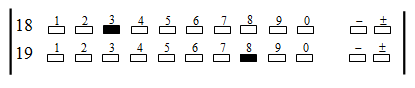
\includegraphics[width=8cm]{415x88-1.png} \\
                     
                     \vspace{0.5cm}
                     例:若第C題的答案格式是 $\underline{\ \FR{\textcps{20}\textcps{21}}{50}\ }$,而答案是 $\FR{-7}{50}$ 時,則考生必須分別在答案卡的第$20$列的 - 與第$21$列的 7 劃記,如:
                     
                         \hspace{2cm} 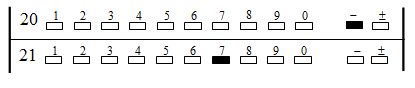
\includegraphics[width=8cm]{415x88-2.png} 
        \end{minipage} 
        }}
\vspace{1cm}
%下方補習班通訊方式
\begin{flushleft}
    \small
        \begin{tabular}{llll}
         {\HWHH 台中總部}:& 台中市北區三民路三段125號 1 樓  & 04-22270156 &【全新教學旗艦中心。光南大批發旁】\\
         {\HWHH 豐原分部}:& 台中市豐原區中正路33號6F		  & 04-25130567 &【豐原火車站旁,諾貝爾書局正對面大樓】
        \end{tabular}
    \end{flushleft}
\end{titlepage}

%引入考卷標頭
%\input{QuizTitle.tex}

%設定三大題區塊
\setlength{\parindent}{0pt} %% 首行不縮排
% !TEX encoding = UTF-8 Unicode
% !TEX TS-program = xelatex 
\begin{QUESTIONS}
    \begin{QUESTION}
        \begin{ExamInfo}{091}{學測}{單選}{1}
        \end{ExamInfo}
        \begin{ExamAnsRateInfo}{76}{97}{83}{48}
        \end{ExamAnsRateInfo}
        \begin{QBODY}
            設 $P(x,y)$ 為坐標平面上一點,且滿足
            $(x-1)^2 +(y-2)^2 + (x-3)^2 +(y-4)^2 = (3-1)^2 +(4-2)^2$
            ,那麼 $P$ 點的位置在哪裡?
            
            \begin{QOPS} 
                \QOP 第一象限 
                \QOP 第二象限 
                \QOP 第三象限 
                \QOP 第四象限 
                \QOP $x$ 軸或 $y$ 軸上
            \end{QOPS}
        \end{QBODY}
        \begin{QFROMS}
        \end{QFROMS}
        \begin{QTAGS}\QTAG{B4C4二次曲線}\end{QTAGS}
        \begin{QANS}
            (1)
        \end{QANS}
        \begin{QSOLLIST}
        \end{QSOLLIST}
        \begin{QEMPTYSPACE}
        \end{QEMPTYSPACE}
    \end{QUESTION}
    \begin{QUESTION}
        \begin{ExamInfo}{091}{學測}{單選}{2}
        \end{ExamInfo}
        \begin{ExamAnsRateInfo}{51}{79}{51}{23}
        \end{ExamAnsRateInfo}
        \begin{QBODY}
            一群登山友,在山上發現一顆巨樹,隊中 $10$ 位身高 $170$ 公分的男生,手拉著手剛好環抱大樹一 圈。問樹幹的直徑最接近下列何值? 
            \begin{QOPS} 
                \QOP $3$公尺 
                \QOP $5$公尺
                \QOP $7$公尺 
                \QOP $9$公尺 
                \QOP $11$ 公尺
            \end{QOPS}
        \end{QBODY}
        \begin{QFROMS}
        \end{QFROMS}
        \begin{QTAGS}\QTAG{綜合}\end{QTAGS}
        \begin{QANS}
            (2)
        \end{QANS}
        \begin{QSOLLIST}
        \end{QSOLLIST}
        \begin{QEMPTYSPACE}
        \end{QEMPTYSPACE}
    \end{QUESTION}
    \begin{QUESTION}
        \begin{ExamInfo}{091}{學測}{單選}{3}
        \end{ExamInfo}
        \begin{ExamAnsRateInfo}{62}{94}{65}{27}
        \end{ExamAnsRateInfo}
        \begin{QBODY}
            如圖,下面哪一選項中的向量與另兩個向量 $\lvec{PO}$, $\lvec{QO}$ 之和等於零向量?
            \begin{QOPS} 
                \QOP $\lvec{AO}$ 
                \QOP $\lvec{BO}$ 
                \QOP $\lvec{CO}$ 
                \QOP $\lvec{DO}$ 
                \QOP $\lvec{EO}$ 
            \end{QOPS}

                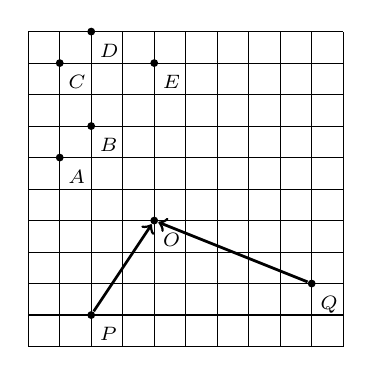
\begin{tikzpicture}[scale=.4]
                \draw (0,0) grid (10,10);\scriptsize
                \foreach \v/\x/\y in {P/2/1,Q/9/2,O/4/4,A/1/6,B/2/7,C/1/9,D/2/10,E/4/9}
                \node[fill,inner sep=1pt,circle] (v\v) at (\x,\y)[label=280:$\v$] {};
                \foreach \i/\j in {P/O, Q/O}
                \draw[->,line width=1pt] (v\i) to (v\j);
                \end{tikzpicture}

        \end{QBODY}
        \begin{QFROMS}
        \end{QFROMS}
        \begin{QTAGS}\QTAG{B3C3平面向量}\end{QTAGS}
        \begin{QANS}
            (3)
        \end{QANS}
        \begin{QSOLLIST}
        \end{QSOLLIST}
        \begin{QEMPTYSPACE}
        \end{QEMPTYSPACE}
    \end{QUESTION}
    \begin{QUESTION}
        \begin{ExamInfo}{091}{學測}{單選}{4}
        \end{ExamInfo}
        \begin{ExamAnsRateInfo}{35}{60}{27}{18}
        \end{ExamAnsRateInfo}
        \begin{QBODY}
            若某校 $1000$ 位學生的數學段考成績平均分數是 $65.24$ 分,樣本標準差是 $5.24$ 分,而且已知成績分佈呈現常態分配。試問全校約有多少人數學成績低於 $60$ 分?
            \begin{QOPS}
                \QOP 約$80$人  
                \QOP 約$160$人 
                \QOP 約$240$人 
                \QOP 約$320$人 
                \QOP 約$400$人
            \end{QOPS}
        \end{QBODY}
        \begin{QFROMS}
        \end{QFROMS}
        \begin{QTAGS}\QTAG{B5C1機率與統計}\end{QTAGS}
        \begin{QANS}
            (2)
        \end{QANS}
        \begin{QSOLLIST}
        \end{QSOLLIST}
        \begin{QEMPTYSPACE}
        \end{QEMPTYSPACE}
    \end{QUESTION}
    \begin{QUESTION}
        \begin{ExamInfo}{091}{學測}{單選}{5}
        \end{ExamInfo}
        \begin{ExamAnsRateInfo}{52}{82}{54}{20}
        \end{ExamAnsRateInfo}
        \begin{QBODY}
            試問用下列哪一個函數的部分圖形來描述右圖較恰當?
            \begin{QOPS}
            \QOP $(x-2)^{2}-2$  
            \QOP $2\sin(x)+2$
            \QOP $2\cos(x)$ 
            \QOP $-0.5(x-2)^{2}+4$ 
            \QOP $3-2^{x}$ 
            \end{QOPS}
            \begin{tikzpicture}[scale=.5]
                \begin{scope}\scriptsize
                \draw[->] (0,-1) to (0,5) node[above] {$y$};
                \draw[->] (-1,0) to (5,0) node[right] {$x$};
                \node[] at (1,-.6) {$(1,0)$};
                \node[] at (-1,1) {$(0,1)$};
                \node[draw,fill,circle,inner sep=1pt] at (0,1) {};
                \node[draw,fill,circle,inner sep=1pt] at (1,0) {};
                \draw[smooth,samples=100,domain=0:5] plot(\x,{-.5*(\x-2)*(\x-2)+4});
                %\draw[smooth,samples=100] (3,3) ellipse (2cm and 4cm) ;
                \end{scope}
            \end{tikzpicture}
        \end{QBODY}
        \begin{QFROMS}
        \end{QFROMS}
        \begin{QTAGS}\QTAG{綜合}\end{QTAGS}
        \begin{QANS}
            (4)
        \end{QANS}
        \begin{QSOLLIST}
        \end{QSOLLIST}
        \begin{QEMPTYSPACE}
        \end{QEMPTYSPACE}
    \end{QUESTION}
    \begin{QUESTION}
        \begin{ExamInfo}{091}{學測}{單選}{6}
        \end{ExamInfo}
        \begin{ExamAnsRateInfo}{33}{53}{32}{14}
        \end{ExamAnsRateInfo}
        \begin{QBODY}
            在坐標平面上有一橢圓,它的長軸落在 $x$ 軸上,短軸落在 $y$ 軸上,長軸、短軸的長度分別為 $4$、$2$。
            如圖所示,通過橢圓的中心 $O$ 且與 $x$ 軸夾角為 $45$ 度的直線在第一象限跟橢圓相交於 $P$。 則此交點 $P$ 與中心 $O$ 的距離為 
            
            
            \begin{QOPS} 
                \QOP $1.5$
                \QOP $\sqrt{1.6}$ 
                \QOP $\sqrt{2}$ 
                \QOP $\sqrt{2.5}$ 
                \QOP $
                \sqrt{3.2}$
            \end{QOPS}
        
            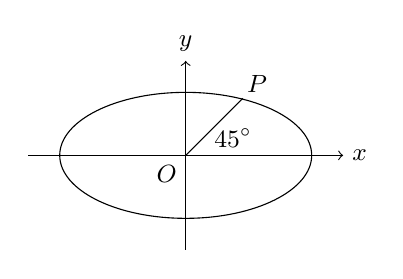
\begin{tikzpicture}[scale=.8]
            \begin{scope}\small
            \draw[->] (0,-1.5) to (0,1.5) node[above] {$y$};
            \draw[->] (-2.5,0) to (2.5,0) node[right] {$x$};
            \node (vO) at (-.3,-.3) {$O$};
            %\draw[smooth,samples=100,domain=.5:2.5] (plot(\x,{2.3*sqrt(\x-.5)});
            \draw (0,0) to (45:1.28);
            \node (vP) at (45:1.6) {$P$};
            \node (vP) at (20:.8) {$45^{\circ}$};
            \draw[smooth,samples=100] (0,0) ellipse (2cm and 1cm) ;
            \end{scope}
            \end{tikzpicture}
            
        \end{QBODY}
        \begin{QFROMS}
        \end{QFROMS}
        \begin{QTAGS}\QTAG{B4C4二次曲線}\end{QTAGS}
        \begin{QANS}
            (2)
        \end{QANS}
        \begin{QSOLLIST}
        \end{QSOLLIST}
        \begin{QEMPTYSPACE}
        \end{QEMPTYSPACE}
    \end{QUESTION}
\end{QUESTIONS}
\begin{QUESTIONS}
    \begin{QUESTION}
        \begin{ExamInfo}{091}{學測}{多選}{7}
        \end{ExamInfo}
        \begin{ExamAnsRateInfo}{75}{93}{82}{50}
        \end{ExamAnsRateInfo}
        \begin{QBODY}
            若實數 $a,b,c$ 滿足 $abc>0$, $ab+bc+ca<0$, $a+b+c>0$, $a>b>c$ ,則下列選項何者為真? 
            \begin{QOPS} 
                \QOP $a>0$ 
                \QOP $b>0$ 
                \QOP $c>0$
                \QOP $|a|>|b|$ 
                \QOP $a^2>c^2$
            \end{QOPS}
        \end{QBODY}
        \begin{QFROMS}
        \end{QFROMS}
        \begin{QTAGS}\QTAG{綜合}\end{QTAGS}
        \begin{QANS}
            (1)(4)(5)
        \end{QANS}
        \begin{QSOLLIST}
        \end{QSOLLIST}
        \begin{QEMPTYSPACE}
        \end{QEMPTYSPACE}
    \end{QUESTION}
    \begin{QUESTION}
        \begin{ExamInfo}{091}{學測}{多選}{8}
        \end{ExamInfo}
        \begin{ExamAnsRateInfo}{60}{88}{64}{28}
        \end{ExamAnsRateInfo}
        \begin{QBODY}
            一機器狗每秒鐘前進或者後退一步,程式設計師讓機器狗以前進 $3$ 步,然後再後退 $2$ 步的規律移動。如果將此機器狗放在數線的原點,面向正的方向,以 $1$ 步的距離為 $1$ 單位長。令 $P(n)$ 表示第 $n$ 秒時機器狗所在位置的坐標,且 $P(0)=0$。那麼下列選項何者為真? 
            \begin{QOPS}
                \QOP $P(3)=3$ 
                \QOP $P(5)=1$ 
                \QOP $P(10)=2$
                \QOP $P(101)=21$ 
                \QOP $P(103)<P(104)$
            \end{QOPS}
        \end{QBODY}
        \begin{QFROMS}
        \end{QFROMS}
        \begin{QTAGS}\QTAG{B2C1數列級數}\end{QTAGS}
        \begin{QANS}
            (1)(2)(3)(4)
        \end{QANS}
        \begin{QSOLLIST}
        \end{QSOLLIST}
        \begin{QEMPTYSPACE}
        \end{QEMPTYSPACE}
    \end{QUESTION}
    \begin{QUESTION}
        \begin{ExamInfo}{091}{學測}{多選}{9}
        \end{ExamInfo}
        \begin{ExamAnsRateInfo}{31}{53}{26}{14}
        \end{ExamAnsRateInfo}
        \begin{QBODY}
            下列哪些選項與方程組 $\left\{ \begin{array}{l} 2x+y+3z=0 \\ 4x+3y+6z =0 \end{array}\right.$ 的解集合相同?
            
            \begin{QOPS} 
                \QOP $y=0$ 
                
                \QOP 
                $\left\{ \begin{array}{l} 2x+3z=0 \\y=0 \end{array}\right.$
                
                \QOP
                $x=y=0$
                
                \QOP
                $\left\{ \begin{array}{l} x+\frac{1}{2}y+\frac{3}{2}z=0 \\ 4x+3y+6z =0 \end{array}\right.$
                
                \QOP
                $\left\{ \begin{array}{l} 6x+4y+9z=0 \\ 2x+y+3z =0 \end{array}\right.$
            \end{QOPS}
        \end{QBODY}
        \begin{QFROMS}
        \end{QFROMS}
        \begin{QTAGS}\QTAG{B4C3矩陣}\end{QTAGS}
        \begin{QANS}
            (2)(4)(5)
        \end{QANS}
        \begin{QSOLLIST}
        \end{QSOLLIST}
        \begin{QEMPTYSPACE}
        \end{QEMPTYSPACE}
    \end{QUESTION}
    \begin{QUESTION}
        \begin{ExamInfo}{091}{學測}{多選}{10}
        \end{ExamInfo}
        \begin{ExamAnsRateInfo}{20}{40}{11}{9}
        \end{ExamAnsRateInfo}
        \begin{QBODY}
            觀察相關的函數圖形,判斷下列選項何者為真?
            \begin{QOPS}
                \QOP $10^x=x$ 有實數解 
                \QOP $10^x=x^2$ 有實數解 
                \QOP $x$ 為實數時,$10^x>x$ 恆成立 
                \QOP $x>0$ 時,$10^x>x^2$ 恆成立 
                \QOP $10^x= -x$ 有實數解
            \end{QOPS}
        \end{QBODY}
        \begin{QFROMS}
        \end{QFROMS}
        \begin{QTAGS}\QTAG{B1C3指對數函數}\end{QTAGS}
        \begin{QANS}
            (2)(3)(4)(5)
        \end{QANS}
        \begin{QSOLLIST}
        \end{QSOLLIST}
        \begin{QEMPTYSPACE}
        \end{QEMPTYSPACE}
    \end{QUESTION}
    \begin{QUESTION}
        \begin{ExamInfo}{091}{學測}{多選}{11}
        \end{ExamInfo}
        \begin{ExamAnsRateInfo}{16}{30}{12}{6}
        \end{ExamAnsRateInfo}
        \begin{QBODY}
            某甲自 $89$ 年 $7$ 月起,每月 $1$ 日均存入銀行 $1000$ 元,言明以月利率 $0.5\%$ 按月複利計息,到 $90$ 年 $7$ 月 $1$ 日提出。某乙則於 $89$ 年 $7$ 月起,每單月(一月、三月、五月 $\cdots$) 1 日均存入 銀行 $2000$ 元,亦以月利率 $0.5\%$ 按月複利計息,到 $90$ 年 $7$ 月 $1$ 日提出。一整年中,兩人都存 入本金 $12000$ 元。提出時,甲得本利和 $A$ 元,乙得本利和 $B$ 元。問下列選項何者為真? 
            \begin{QOPS} 
                \QOP $B>A$ 
                \QOP $A= 1000\cdot [\Sum_{k=1}^{12} (1.005)^k ]$ 
                \QOP $B= 2000 [\Sum_{k=1}^{6} (1.005)^{2k}] $ 
                \QOP $A< 12000 (1.005)^{12}$  
                \QOP $B< 12000 (1.005)^{12}$
            \end{QOPS}
        \end{QBODY}
        \begin{QFROMS}
        \end{QFROMS}
        \begin{QTAGS}\QTAG{B2C1數列級數}\end{QTAGS}
        \begin{QANS}
            (1)(2)(3)(4)(5)
        \end{QANS}
        \begin{QSOLLIST}
        \end{QSOLLIST}
        \begin{QEMPTYSPACE}
        \end{QEMPTYSPACE}
    \end{QUESTION}
    \begin{QUESTION}
        \begin{ExamInfo}{091}{學測}{多選}{12}
        \end{ExamInfo}
        \begin{ExamAnsRateInfo}{36}{67}{29}{12}
        \end{ExamAnsRateInfo}
        \begin{QBODY}
            在 $\triangle ABC$ 中,下列哪些選項的條件有可能成立?
            \begin{QOPS} 
                \QOP $\sin A=\sin B= \sin C= \frac{\sqrt{3}}{2}$ 
                \QOP $\sin A$, $\sin B$, $\sin C$ 均小於 $\frac{1}{2}$ 
                \QOP $\sin A, \sin B$, $\sin C$ 均大於 $\frac{\sqrt{3}}{2}$ 
                \QOP $\sin A = \sin B = \sin C =\frac{1}{2}$ 
                \QOP $\sin A= \sin B= \frac{1}{2}$ , $\sin C= \frac{\sqrt{3}}{2}$
            \end{QOPS}
        \end{QBODY}
        \begin{QFROMS}
        \end{QFROMS}
        \begin{QTAGS}\QTAG{B3C1三角}\end{QTAGS}
        \begin{QANS}
            (1)(2)(5)
        \end{QANS}
        \begin{QSOLLIST}
        \end{QSOLLIST}
        \begin{QEMPTYSPACE}
        \end{QEMPTYSPACE}
    \end{QUESTION}
\end{QUESTIONS}
\begin{QUESTIONS}
    \begin{QUESTION}
        \begin{ExamInfo}{091}{學測}{填充}{A}
        \end{ExamInfo}
        \begin{ExamAnsRateInfo}{28}{65}{17}{2}
        \end{ExamAnsRateInfo}
        \begin{QBODY}
            工匠在窗子外邊想做一個圓弧型的花台,
            此花台在窗口的中央往外伸出 72 公分,
            窗口的寬度是 168 公分,
            則此圓弧的圓半徑為 
            \TCNBOX{\TCN\TCN} 公分。
        \end{QBODY}
        \begin{QFROMS}
        \end{QFROMS}
        \begin{QTAGS}\QTAG{B3C2直線與圓}\end{QTAGS}
        \begin{QANS}
            $85$
        \end{QANS}
        \begin{QSOLLIST}
        \end{QSOLLIST}
        \begin{QEMPTYSPACE}
        \end{QEMPTYSPACE}
    \end{QUESTION}
    \begin{QUESTION}
        \begin{ExamInfo}{091}{學測}{填充}{B}
        \end{ExamInfo}
        \begin{ExamAnsRateInfo}{50}{70}{51}{29}
        \end{ExamAnsRateInfo}
        \begin{QBODY}
            $2^{20}-1$ 與 $2^{19}+1$ 的最大公因數為 
            \TCNBOX{\TCN}
        \end{QBODY}
        \begin{QFROMS}
        \end{QFROMS}
        \begin{QTAGS}\QTAG{綜合}\end{QTAGS}
        \begin{QANS}
            $3$
        \end{QANS}
        \begin{QSOLLIST}
        \end{QSOLLIST}
        \begin{QEMPTYSPACE}
        \end{QEMPTYSPACE}
    \end{QUESTION}
    \begin{QUESTION}
        \begin{ExamInfo}{091}{學測}{填充}{C}
        \end{ExamInfo}
        \begin{ExamAnsRateInfo}{38}{70}{32}{12}
        \end{ExamAnsRateInfo}
        \begin{QBODY}
            某公司民國 $85$ 年營業額為 $4$ 億元,民國 $86$ 年營業額為 $6$ 億元,該年的成長率為 $50\%$。 $87$、$88$、$89$ 三年的成長率皆相同,且民國 $89$ 年的營業額為 48 億元。則該公司 89 年的成長率為 
            $\TCNBOX{\TCN\TCN\TCN} \%$
        \end{QBODY}
        \begin{QFROMS}
        \end{QFROMS}
        \begin{QTAGS}\QTAG{B2C1數列級數}\end{QTAGS}
        \begin{QANS}
            $100\%$
        \end{QANS}
        \begin{QSOLLIST}
        \end{QSOLLIST}
        \begin{QEMPTYSPACE}
        \end{QEMPTYSPACE}
    \end{QUESTION}
    \begin{QUESTION}
        \begin{ExamInfo}{091}{學測}{填充}{D}
        \end{ExamInfo}
        \begin{ExamAnsRateInfo}{50}{67}{53}{30}
        \end{ExamAnsRateInfo}
        \begin{QBODY}
            在一個圓的圓周上,平均分佈了 $60$ 個洞,兩洞間稱為一間隔。在 $A$ 洞打上一支木樁並綁上線,然後依逆時針方向前進每隔 $9$ 個間隔就再打一支木樁,並綁上線,依此繼續操作,如右圖所示。 試問輪回到 $A$ 洞需再打樁前,總共已經打了$\TCNBOX{{\TCN\TCN}}$支木樁。\\
            
            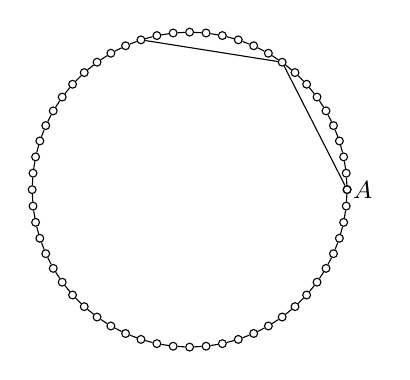
\begin{tikzpicture}[scale=.4]
            \begin{scope}
            \foreach \i in {0,1,2,...,59,60}
            \node[draw,circle,inner sep=1pt]  (v\i) at (6*\i:5) {};
            \foreach \i [remember=\i as \lasti (initially 0)] in {1,2,...,60}
            \draw (v\i) to (v\lasti);
            \draw (v0) to (v9);
            \draw (v9) to (v18);
            \node at (5.5,0) {\small $A$};
            \end{scope}
            \end{tikzpicture}
        \end{QBODY}
        \begin{QFROMS}
        \end{QFROMS}
        \begin{QTAGS}\QTAG{綜合}\end{QTAGS}
        \begin{QANS}
            $20$
        \end{QANS}
        \begin{QSOLLIST}
        \end{QSOLLIST}
        \begin{QEMPTYSPACE}
        \end{QEMPTYSPACE}
    \end{QUESTION}
    \begin{QUESTION}
        \begin{ExamInfo}{091}{學測}{填充}{E}
        \end{ExamInfo}
        \begin{ExamAnsRateInfo}{41}{70}{41}{12}
        \end{ExamAnsRateInfo}
        \begin{QBODY}
            某次網球比賽共有 $128$ 位選手參加,採單淘汰制,每輪淘汰一半的選手,剩下一半的選手進入下一輪。在第 $1$ 輪被淘汰的選手可獲得 $1$ 萬元,在第 $2$ 輪被淘汰的選手可獲得 $2$ 萬元,在第 $k$ 輪被淘汰的選手可獲得 $2^{k-1}$ 萬元,而冠軍則可獲得 $128$ 萬元。試問全部比賽獎金共$\TCNBOX{\TCN\TCN\TCN}$萬元。
        \end{QBODY}
        \begin{QFROMS}
        \end{QFROMS}
        \begin{QTAGS}\QTAG{B2C1數列級數}\end{QTAGS}
        \begin{QANS}
            $576$萬元
        \end{QANS}
        \begin{QSOLLIST}
        \end{QSOLLIST}
        \begin{QEMPTYSPACE}
        \end{QEMPTYSPACE}
    \end{QUESTION}
    \begin{QUESTION}
        \begin{ExamInfo}{091}{學測}{填充}{F}
        \end{ExamInfo}
        \begin{ExamAnsRateInfo}{51}{89}{50}{14}
        \end{ExamAnsRateInfo}
        \begin{QBODY}
            某人隔河測一山高,在 $A$ 點觀測山時,山的方位為東偏北 $60^\circ$,
            山頂的仰角為 $45^\circ$,
            某人自 $A$ 點向東行 $600$ 公尺到達 $B$ 點,山的方位變成在西偏北 $60^\circ$,則山有多高? 答: $
            \TCNBOX{\TCN\TCN\TCN}$ 公尺。
        \end{QBODY}
        \begin{QFROMS}
        \end{QFROMS}
        \begin{QTAGS}\QTAG{B3C1三角}\end{QTAGS}
        \begin{QANS}
            $600$
        \end{QANS}
        \begin{QSOLLIST}
        \end{QSOLLIST}
        \begin{QEMPTYSPACE}
        \end{QEMPTYSPACE}
    \end{QUESTION}
    \begin{QUESTION}
        \begin{ExamInfo}{091}{學測}{填充}{G}
        \end{ExamInfo}
        \begin{ExamAnsRateInfo}{29}{58}{24}{5}
        \end{ExamAnsRateInfo}
        \begin{QBODY}
            有一群體有九位成員,其身高分別為(單位:公分) $160, 163, 166, 170, 172, 174, 176, 178, 180$ , 此九人的平均身高為 $171$ 公分。今隨機抽樣 $3$ 人,則抽到 $3$ 人的平均身高等於母體平均身高的機率為 
            $\TCNBOX{\FR{\TCN}{\TCN\TCN}} $。
        \end{QBODY}
        \begin{QFROMS}
        \end{QFROMS}
        \begin{QTAGS}\QTAG{B2C4數據分析}\end{QTAGS}
        \begin{QANS}
            $\frac{1}{28}$
        \end{QANS}
        \begin{QSOLLIST}
        \end{QSOLLIST}
        \begin{QEMPTYSPACE}
        \end{QEMPTYSPACE}
    \end{QUESTION}
    \begin{QUESTION}
        \begin{ExamInfo}{091}{學測}{填充}{H}
        \end{ExamInfo}
        \begin{ExamAnsRateInfo}{28}{69}{14}{1}
        \end{ExamAnsRateInfo}
        \begin{QBODY}
            右圖為一正立方體,被一平面截出一個四邊形 $ABCD$,
            其中 $B,D$ 分別為稜的中點,
            且 $\overline{EA}: \overline{AF}=1:2$,則 $\cos\angle DAB= $ 
            $\TCNBOX{\FR{\TCN}{\TCN\TCN}}$
            
            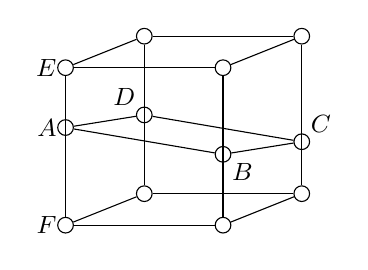
\begin{tikzpicture}
                \small
                \tikzstyle{vnode}=[draw,circle,inner sep =2pt];
                \node[vnode] (v000) at (0,0) {};
                \node[anchor =east] (t000) at (v000) {};
                \node[vnode] (v001) at (0,2) {};
                \node[anchor =east] (t000) at (v001) {};
                \node[vnode] (v011) at (2,2) {};
                \node[anchor =west] (t011) at (v011) {};
                \node[vnode] (v010) at (2,0) {};
                \node[anchor =west] (t010) at (v010) {};
                \node[vnode] (v100) at (-1.0,-.4) {};
                \node[anchor =east] (t100) at (v100) {$F$};
                \node[vnode] (v101) at (-1.0,1.6) {};
                \node[anchor =east] (t101) at (v101) {$E$};
                \node[vnode] (v111) at (1.0,1.6) {};
                \node[anchor =north east] (t111) at (v111) {};
                \node[vnode] (v110) at (1.0,-0.4) {};
                \node[anchor =west] (t110) at (v110) {};
                \node[vnode] (vA) at (-1,.84) {};
                \node[anchor =east] (tA) at (vA) {$A$};
                \node[vnode] (vC) at (2,.66) {};
                \node[anchor =south west] (tC) at (vC) {$C$};
                \node[vnode] (vD) at (0,1) {};
                \node[anchor =south east] (tD) at (vD) {$D$};
                \node[vnode] (vB) at (1,.5) {};
                \node[anchor =north west] (tB) at (vB) {$B$};
                \draw (vD) to[dashed] (vA);
                \draw (vD) to[dashed] (vC);
                \draw (vB) to (vA);
                \draw (vB) to (vC);
                \foreach \i in {01,10,11}{
                    \draw (v0\i) to (v1\i);
                    \draw (v\i  0) to (v\i 1);
                }
                \draw (v000) to[dashed] (v100);
                \draw (v000) to[dashed] (v010);
                \draw (v000) to[dashed] (v001);
                \draw (v001) to (v011);
                \draw (v100) to (v110);
                \draw (v101) to (v111);              
            \end{tikzpicture}
            
        \end{QBODY}
        \begin{QFROMS}
        \end{QFROMS}
        \begin{QTAGS}\QTAG{B4C1空間向量}\end{QTAGS}
        \begin{QANS}
            $\frac{1}{37}$
        \end{QANS}
        \begin{QSOLLIST}
        \end{QSOLLIST}
        \begin{QEMPTYSPACE}
        \end{QEMPTYSPACE}
    \end{QUESTION}
\end{QUESTIONS}

    \begin{QUESTION}
        \begin{ExamInfo}{92}{學測}{單選}{1}
        \end{ExamInfo}
        \begin{ExamAnsRateInfo}{46}{74}{46}{18}
        \end{ExamAnsRateInfo}
        \begin{QBODY}
            試問有多少個正整數 $n$ 使得 $ \dfrac{1}{n} + \dfrac{2}{n} + \cdots + \dfrac{10}{n}$ 為整數? 
            \begin{QOPS} 
                \QOP $1$ 個 
                \QOP $2$ 個  
                \QOP $3$ 個 
                \QOP $4$ 個 
                \QOP $5$ 個
            \end{QOPS}
        \end{QBODY}
        \begin{QFROMS}
        \end{QFROMS}
        \begin{QTAGS}\QTAG{B2C1數列級數}\QTAG{B2C1-2級數}\end{QTAGS}
        \begin{QANS}
            (4)
        \end{QANS}
        \begin{QSOLLIST}
        \end{QSOLLIST}
        \begin{QEMPTYSPACE}
        \end{QEMPTYSPACE}
    \end{QUESTION}
    \begin{QUESTION}
        \begin{ExamInfo}{92}{學測}{單選}{2}
        \end{ExamInfo}
        \begin{ExamAnsRateInfo}{46}{83}{44}{11}
        \end{ExamAnsRateInfo}
        \begin{QBODY}
            若 $f(x)=x^3 - 2x^2 -x +5$,則多項式 $g(x)=f(f(x))$ 除以$(x-2)$ 所得的餘式為 
            \begin{QOPS} 
                \QOP $3 $
                \QOP $5 $
                \QOP $7 $
                \QOP $9 $
                \QOP $11$
            \end{QOPS}
        \end{QBODY}
        \begin{QFROMS}
        \end{QFROMS}
        \begin{QTAGS}\QTAG{B1C2多項式函數}\QTAG{B1C2-2多項式的運算與應用}\QTAG{餘式定理}\end{QTAGS}
        \begin{QANS}
            (5)
        \end{QANS}
        \begin{QSOLLIST}
        \end{QSOLLIST}
        \begin{QEMPTYSPACE}
        \end{QEMPTYSPACE}
    \end{QUESTION}
    \begin{QUESTION}
        \begin{ExamInfo}{92}{學測}{單選}{3}
        \end{ExamInfo}
        \begin{ExamAnsRateInfo}{41}{66}{36}{21}
        \end{ExamAnsRateInfo}
        \begin{QBODY}
            若 $(4 + 3i)(\cos \theta + i \sin \theta )$ 為小於 0 的實數, 則 $\theta$ 是第幾象限角? 
            \begin{QOPS} 
                \QOP 第一象限角 
                \QOP 第二象限角 
                \QOP 第三象限角 
                \QOP 第四象限角 
                \QOP 條件不足,無法判斷
            \end{QOPS}
        \end{QBODY}
        \begin{QFROMS}
        \end{QFROMS}
        \begin{QTAGS}\QTAG{B5C2三角函數II}\end{QTAGS}
        \begin{QANS}
            (2)
        \end{QANS}
        \begin{QSOLLIST}
        \end{QSOLLIST}
        \begin{QEMPTYSPACE}
        \end{QEMPTYSPACE}
    \end{QUESTION}
    \begin{QUESTION}
        \begin{ExamInfo}{92}{學測}{單選}{4}
        \end{ExamInfo}
        \begin{ExamAnsRateInfo}{49}{69}{47}{31}
        \end{ExamAnsRateInfo}
        \begin{QBODY}
            設 $ABC$ 為坐標平面上一三角形,$P$ 為平面上一點且 $\lvec{AP} = \dfrac{1}{5} \lvec{AB} + \dfrac{2}{5} \lvec{AC}$ , 則 $\dfrac{\triangle ABP \mbox{面積}}{ \triangle ABC \mbox{面積}}$等於 
            \begin{QOPS}
                \QOP $\dfrac{1}{5}$ 
                \QOP $\dfrac{1}{4}$ 
                \QOP $\dfrac{2}{5}$ 
                \QOP $\dfrac{1}{2}$         
                \QOP $\dfrac{2}{3}$
            \end{QOPS}
        \end{QBODY}
        \begin{QFROMS}
        \end{QFROMS}
        \begin{QTAGS}\QTAG{面積}\QTAG{B3C3-3面積與二階行列式}\QTAG{B3C3-1平面向量的表示法}\QTAG{B3C3平面向量}\QTAG{線性組合}\end{QTAGS}
        \begin{QANS}
            (3)
        \end{QANS}
        \begin{QSOLLIST}
        \end{QSOLLIST}
        \begin{QEMPTYSPACE}
        \end{QEMPTYSPACE}
    \end{QUESTION}
    \begin{QUESTION}
        \begin{ExamInfo}{92}{學測}{單選}{5}
        \end{ExamInfo}
        \begin{ExamAnsRateInfo}{22}{43}{15}{8}
        \end{ExamAnsRateInfo}
        \begin{QBODY}
            根據統計資料,在  $A$ 小鎮當某件訊息發布後, 
            $t$ 小時之內聽到該訊息的人口是全鎮人口的 $100(1- 2^{-kt})\%$ ,
            其中 $k$ 是某個大於 $0$ 的常數。
            今有某訊息,假設在發布後 $3$ 小時之內已經有 $70\%$ 的人口聽到該訊息。
            又設最快要 $T$ 小時後,有 $99\%$ 的人口已聽到該訊息,則 $T$ 最接近下列哪一個選項?
            \begin{QOPS} 
                \QOP $5$小時        
                \QOP $7\frac{1}{2}$小時
                \QOP $9$小時 
                \QOP $11\frac{1}{2}$小時 
                \QOP $13$小時
            \end{QOPS}
        \end{QBODY}
        \begin{QFROMS}
        \end{QFROMS}
        \begin{QTAGS}\QTAG{應用問題}\QTAG{B1C3指對數函數}\QTAG{B1C3-5指數與對數的應用}\end{QTAGS}
        \begin{QANS}
            (4)
        \end{QANS}
        \begin{QSOLLIST}
        \end{QSOLLIST}
        \begin{QEMPTYSPACE}
        \end{QEMPTYSPACE}
    \end{QUESTION}
    \begin{QUESTION}
        \begin{ExamInfo}{92}{學測}{多選}{6}
        \end{ExamInfo}
        \begin{ExamAnsRateInfo}{41}{71}{40}{12}
        \end{ExamAnsRateInfo}
        \begin{QBODY}
            如右圖,兩直線 $L_1$ 、 $L_2$ 之方程式分別為 $L_1 : x+ay+b=0$, $L_2 :x+cy+d=0$;試問下列哪些選項是正確的? 
            \begin{QOPS} 
                \QOP $a>0$ 
                \QOP $b>0$ 
                \QOP $c>0$ 
                \QOP $d>0$ 
                \QOP $a<c$ 
            \end{QOPS}
            
            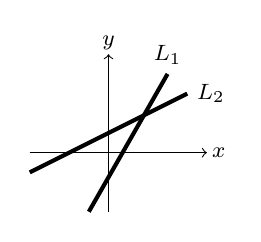
\begin{tikzpicture}[scale=.5]\footnotesize
            \begin{scope}
            \pgfsetarrowsend{latex}
            \draw[->]  (-2,0) to(2.5,0);
            \draw[->] (0,-1.5) to (0,2.5);
            \end{scope}
            \pgfsetlinewidth{1.5pt}
            \node at (0,2.8) {$y$};
            \node at (2.8,0) {$x$};
            \draw (-2,-0.5) to (2,1.5) node[right] {$L_2$};
            \draw (-.5,-1.5) to (1.5,2)node[above] {$L_1$} ;
            \end{tikzpicture}
        \end{QBODY}
        \begin{QFROMS}
        \end{QFROMS}
        \begin{QTAGS}\QTAG{B3C2-1直線方程式及其圖形}\QTAG{圖形}\QTAG{B3C2直線與圓}\end{QTAGS}
        \begin{QANS}
            (4)(5)
        \end{QANS}
        \begin{QSOLLIST}
        \end{QSOLLIST}
        \begin{QEMPTYSPACE}
        \end{QEMPTYSPACE}
    \end{QUESTION}
    \begin{QUESTION}
        \begin{ExamInfo}{92}{學測}{多選}{7}
        \end{ExamInfo}
        \begin{ExamAnsRateInfo}{45}{79}{41}{15}
        \end{ExamAnsRateInfo}
        \begin{QBODY}
            如右圖,$ABCD-EFGH$ 為一平行六面體,$J$ 為四邊形 $BCGF$ 的中心,
            如果 $\lvec{AJ} = a \lvec{AB} + b\lvec{AD}+ c\lvec{AE}$,
            試問下列哪些選項是正確的? 
            \begin{QOPS} 
                \QOP $\frac{1}{3} < b < \frac{2}{3}$ 
                \QOP $a + b + c = 2$  
                \QOP $a=1$
                \QOP $a=2c$ 
                \QOP $a=b$
            \end{QOPS}
        
            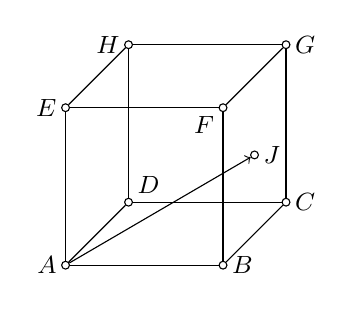
\begin{tikzpicture}
                \begin{scope}
                \small
                \tikzstyle{vnode}=[draw,circle,inner sep =1pt];
                \node[vnode] (v000) at (0,0) {};
                \node[anchor =south west] (t000) at (v000) {$D$};
                \node[vnode] (v001) at (0,2) {$$};
                \node[anchor =east] (t000) at (v001) {$H$};
                \node[vnode] (v011) at (2,2) {$$};
                \node[anchor =west] (t011) at (v011) {$G$};
                \node[vnode] (v010) at (2,0) {$$};
                \node[anchor =west] (t010) at (v010) {$C$};
                \node[vnode] (v100) at (-.8,-.8) {$$};
                \node[anchor =east] (t100) at (v100) {$A$};
                \node[vnode] (v101) at (-.8,1.2) {$$};
                \node[anchor =east] (t101) at (v101) {$E$};
                \node[vnode] (v111) at (1.2,1.2) {$$};
                \node[anchor =north east] (t111) at (v111) {$F$};
                \node[vnode] (v110) at (1.2,-0.8) {$$};
                \node[anchor =west] (t110) at (v110) {$B$};
                \node[vnode] (vJ) at (1.6, .6) {$$};
                \node[anchor =west] (tJ) at (vJ) {$J$};
                \foreach \i in {01,10,11}{
                    \draw (v0\i) to (v1\i);
                    \draw (v\i  0) to (v\i 1);
                }
                \draw (v000) to[dashed] (v100);
                \draw (v000) to[dashed] (v010);
                \draw (v000) to[dashed] (v001);
                \draw (v001) to (v011);
                \draw (v100) to (v110);
                \draw (v101) to (v111);
                \draw[->] (v100) to (vJ);
                \end{scope}
            \end{tikzpicture}
        \end{QBODY}
        \begin{QFROMS}
        \end{QFROMS}
        \begin{QTAGS}\QTAG{B4C1-2空間向量的坐標表示法}\QTAG{B4C1空間向量}\end{QTAGS}
        \begin{QANS}
            (1)(2)(3)(4)
        \end{QANS}
        \begin{QSOLLIST}
        \end{QSOLLIST}
        \begin{QEMPTYSPACE}
        \end{QEMPTYSPACE}
    \end{QUESTION}
    \begin{QUESTION}
        \begin{ExamInfo}{92}{學測}{多選}{8}
        \end{ExamInfo}
        \begin{ExamAnsRateInfo}{55}{86}{60}{19}
        \end{ExamAnsRateInfo}
        \begin{QBODY}
            以下各數何者為正? 
            \begin{QOPS} 
                \QOP $\sqrt{2} - \sqrt[3]{2}$ 
                \QOP $\log_{2} 3-1$ 
                \QOP $\log_{3}2 -1$ 
                \QOP $\log_{\frac{1}{2}} 3$ 
                \QOP $\log_{\frac{1}{3}} \frac{1}{2}$ 
            \end{QOPS}
        \end{QBODY}
        \begin{QFROMS}
        \end{QFROMS}
        \begin{QTAGS}\QTAG{B1C3-2指數函數}\QTAG{B1C3指對數函數}\QTAG{指數律}\end{QTAGS}
        \begin{QANS}
            (1)(2)(5)
        \end{QANS}
        \begin{QSOLLIST}
        \end{QSOLLIST}
        \begin{QEMPTYSPACE}
        \end{QEMPTYSPACE}
    \end{QUESTION}
    \begin{QUESTION}
        \begin{ExamInfo}{92}{學測}{多選}{9}
        \end{ExamInfo}
        \begin{ExamAnsRateInfo}{24}{42}{19}{11}
        \end{ExamAnsRateInfo}
        \begin{QBODY}
            下列哪些函數的最小正週期為 $\pi$ ? 
            \begin{QOPS} 
                \QOP $\sin x + \cos x$ 
                \QOP $\sin x - \cos x$ 
                \QOP $|\sin x + \cos x|$
                \QOP $|\sin x - \cos x|$ 
                \QOP $|\sin x| + |\cos x|$
            \end{QOPS}
        \end{QBODY}
        \begin{QFROMS}
        \end{QFROMS}
        \begin{QTAGS}\QTAG{B5C2-1一般三角函數的性質與圖形}\QTAG{B5C2三角函數II}\end{QTAGS}
        \begin{QANS}
            (3)(4)
        \end{QANS}
        \begin{QSOLLIST}
        \end{QSOLLIST}
        \begin{QEMPTYSPACE}
        \end{QEMPTYSPACE}
    \end{QUESTION}
    \begin{QUESTION}
        \begin{ExamInfo}{92}{學測}{多選}{10}
        \end{ExamInfo}
        \begin{ExamAnsRateInfo}{21}{43}{14}{6}
        \end{ExamAnsRateInfo}
        \begin{QBODY}
            假設坐標平面上一非空集合 $S$ 試問下列哪些敘述對 $S$ 內的點 $(x, y)$ 具有以下性質:「若  $x > 0$,則 $y > 0$」。 試問下列哪些敘述對 $S$ 內的點 $(x, y)$ 必定成立? 
            \begin{QOPS} 
                \QOP 若 $x \leq 0$,則 $y \leq 0$ ;
                \QOP 若 $y \leq 0$, 則 $x \leq 0$;
                \QOP 若 $y \leq 0$,則 $x \leq 0$ ; 
                \QOP 若 $x >1$,則 $y>0$;  \QOP 若 $y<0$ ,則 $x \leq 0$。
            \end{QOPS}
        \end{QBODY}
        \begin{QFROMS}
        \end{QFROMS}
        \begin{QTAGS}\QTAG{不是99課綱}\end{QTAGS}
        \begin{QANS}
            (2)(4)(5)
        \end{QANS}
        \begin{QSOLLIST}
        \end{QSOLLIST}
        \begin{QEMPTYSPACE}
        \end{QEMPTYSPACE}
    \end{QUESTION}
    \begin{QUESTION}
        \begin{ExamInfo}{92}{學測}{多選}{11}
        \end{ExamInfo}
        \begin{ExamAnsRateInfo}{24}{43}{18}{11}
        \end{ExamAnsRateInfo}
        \begin{QBODY}
            設 $\pi_a : x-4y +az=10$ ($a$為常數), $E_1 :x-2y+z=5$ 及 $E_2  :2x-5y+4z=3$ 為坐標空間中的三個平面。
            試問下列哪些敘述是正確的?
            
            \begin{QOPS} 
                \QOP 存在實數 $a$ 使得 $\pi_a$ 與 $E_1$ 平行;
                \QOP 存在實數 $a$ 使得 $\pi_a$ 與 $E_1$ 垂直;
                \QOP 存在實數 $a$ 使得 $\pi_a$ , $E_1$, $E_2$ 交於一點; 
                \QOP 存在實數 $a$ 使得 $\pi_a, E_1, E_2 $ 交於一直線;
                \QOP 存在實數 $a$ 使得 $\pi_a$, $E_1$ , $E_2$ 沒有共同交點。\end{QOPS}
        \end{QBODY}
        \begin{QFROMS}
        \end{QFROMS}
        \begin{QTAGS}\QTAG{B4C3矩陣}\QTAG{B4C3-1線性方程組與矩陣}\QTAG{方程組}\end{QTAGS}
        \begin{QANS}
            (2)(3)(5)
        \end{QANS}
        \begin{QSOLLIST}
        \end{QSOLLIST}
        \begin{QEMPTYSPACE}
        \end{QEMPTYSPACE}
    \end{QUESTION}
    \begin{QUESTION}
        \begin{ExamInfo}{92}{學測}{填充}{A}
        \end{ExamInfo}
        \begin{ExamAnsRateInfo}{37}{74}{31}{6}
        \end{ExamAnsRateInfo}
        \begin{QBODY}
            設 $a_1,a_2,\cdots,a_{50}$ 是從 $-1,0,1$ 這三個整數中取值的數列。若 $a_1 +a_2 + \cdots + a_{50} = 9$ 且 $(a_1+1)^2 +(a_2 +1)^2 + \cdots + (a_{50} +1)^2 =107$, 則 $a_1,a_2,\cdots,a_{50}$ 當中有幾項是 $0$?答: 
            $\TCNBOX{\TCN\TCN}$ 項。
        \end{QBODY}
        \begin{QFROMS}
        \end{QFROMS}
        \begin{QTAGS}\QTAG{B2C1數列級數}\QTAG{特殊數列}\QTAG{B2C1-2級數}\QTAG{B2C1-1數列}\end{QTAGS}
        \begin{QANS}
            $11$
        \end{QANS}
        \begin{QSOLLIST}
        \end{QSOLLIST}
        \begin{QEMPTYSPACE}
        \end{QEMPTYSPACE}
    \end{QUESTION}
    \begin{QUESTION}
        \begin{ExamInfo}{92}{學測}{填充}{B}
        \end{ExamInfo}
        \begin{ExamAnsRateInfo}{64}{93}{70}{29}
        \end{ExamAnsRateInfo}
        \begin{QBODY}
            金先生在提款時忘了帳號密碼,但他還記得密碼的四位數字中,有兩個 $3$, 一個 $8$,一個 $9$,於是他就用這四個數字隨意排成一個四位數輸入提款機嘗試。請問他只試一次就成功的機率有多少? $\TCNBOX{\FR{\TCN}{\TCN\TCN}}$
        \end{QBODY}
        \begin{QFROMS}
        \end{QFROMS}
        \begin{QTAGS}\QTAG{B2C3機率}\QTAG{B2C3-2機率的定義與性質}\end{QTAGS}
        \begin{QANS}
            $\frac{1}{12}$
        \end{QANS}
        \begin{QSOLLIST}
        \end{QSOLLIST}
        \begin{QEMPTYSPACE}
        \end{QEMPTYSPACE}
    \end{QUESTION}
    \begin{QUESTION}
        \begin{ExamInfo}{92}{學測}{填充}{C}
        \end{ExamInfo}
        \begin{ExamAnsRateInfo}{27}{52}{21}{8}
        \end{ExamAnsRateInfo}
        \begin{QBODY}
            設 $A(1,0)$ 與 $B(b,0)$ 為坐標平面上的兩點, 其中 $b>1$。 
            若拋物線 $\Gamma : y^2=4x$ 上有一點 $P$ 使得 $\triangle ABP$ 為一正三角形,則 $b= 
            \TCNBOX{\TCN}$。
        \end{QBODY}
        \begin{QFROMS}
        \end{QFROMS}
        \begin{QTAGS}\QTAG{B4C4二次曲線}\QTAG{B4C4-1拋物線}\QTAG{圖形}\end{QTAGS}
        \begin{QANS}
            $5$
        \end{QANS}
        \begin{QSOLLIST}
        \end{QSOLLIST}
        \begin{QEMPTYSPACE}
        \end{QEMPTYSPACE}
    \end{QUESTION}
    \begin{QUESTION}
        \begin{ExamInfo}{92}{學測}{填充}{D}
        \end{ExamInfo}
        \begin{ExamAnsRateInfo}{16}{39}{7}{2}
        \end{ExamAnsRateInfo}
        \begin{QBODY}
            設 $P$ 為雙曲線 $\dfrac{x^2}{9} - \dfrac{y^2}{16} = 1$ 上的一點且位在第一象限。若 $F_1$,  $F_2$ 為此雙曲線的兩個焦點,且 $\overline{PF}_1 : \overline{PF}_2 = 1:3 $,則 $\triangle F_1PF_2$ 的周長等於 $
            \TCNBOX{\TCN\TCN}$。
        \end{QBODY}
        \begin{QFROMS}
        \end{QFROMS}
        \begin{QTAGS}\QTAG{B4C4-3雙曲線}\QTAG{B4C4二次曲線}\QTAG{圖形}\end{QTAGS}
        \begin{QANS}
            $22$
        \end{QANS}
        \begin{QSOLLIST}
        \end{QSOLLIST}
        \begin{QEMPTYSPACE}
        \end{QEMPTYSPACE}
    \end{QUESTION}
    \begin{QUESTION}
        \begin{ExamInfo}{92}{學測}{填充}{E}
        \end{ExamInfo}
        \begin{ExamAnsRateInfo}{21}{37}{17}{9}
        \end{ExamAnsRateInfo}
        \begin{QBODY}
            在坐標空間中,通過 $O(0,0,0)$, $N(0,0,1)$, $P(\dfrac{1}{4}, \dfrac{\sqrt{11}}{4}, -\dfrac{1}{2})$ 三點的平面與球面  $S: x^2+y^2+z^2=1$相交於一個圓 $C$,則圓 $C$ 的劣弧 $NP$ 的弧長等於 
            $\TCNBOX{\FR{\TCN}{\TCN} \pi} $。
        \end{QBODY}
        \begin{QFROMS}
        \end{QFROMS}
        \begin{QTAGS}\QTAG{不是99課綱}\end{QTAGS}
        \begin{QANS}
            $\frac{2}{3}\pi$
        \end{QANS}
        \begin{QSOLLIST}
        \end{QSOLLIST}
        \begin{QEMPTYSPACE}
        \end{QEMPTYSPACE}
    \end{QUESTION}
    \begin{QUESTION}
        \begin{ExamInfo}{92}{學測}{填充}{F}
        \end{ExamInfo}
        \begin{ExamAnsRateInfo}{35}{67}{31}{7}
        \end{ExamAnsRateInfo}
        \begin{QBODY}
            設 $k$ 為一整數,若方程式 $kx^2 + 7x +1= 0$ 有兩個相異實根,且兩根的乘積介於 $\dfrac{5}{71}$ 與 $\dfrac{6}{71}$之間,則 $k=\TCNBOX{\TCN\TCN}$。
        \end{QBODY}
        \begin{QFROMS}
        \end{QFROMS}
        \begin{QTAGS}\QTAG{B1C2-3多項式方程式}\QTAG{根與係數的關係}\QTAG{B1C2多項式函數}\QTAG{韋達定理}\end{QTAGS}
        \begin{QANS}
            $12$
        \end{QANS}
        \begin{QSOLLIST}
        \end{QSOLLIST}
        \begin{QEMPTYSPACE}
        \end{QEMPTYSPACE}
    \end{QUESTION}
    \begin{QUESTION}
        \begin{ExamInfo}{92}{學測}{填充}{G}
        \end{ExamInfo}
        \begin{ExamAnsRateInfo}{15}{41}{4}{0}
        \end{ExamAnsRateInfo}
        \begin{QBODY}
            在只有皮尺沒有梯子的情形下,想要測出一拋物線形拱門的高度。
            已知此拋物線以過最高點的鉛垂線為對稱軸。
            現甲、乙兩人以皮尺測得拱門底部寬為 $6$ 公尺,且距底部 $\frac{3}{2}$ 公尺高處其寬為 $5$ 公尺。
            利用這些數據可推算出拱門的高度為$\TCNBOX{\FR{\TCN\TCN}{\TCN\TCN}}$ 公尺。
        \end{QBODY}
        \begin{QFROMS}
        \end{QFROMS}
        \begin{QTAGS}\QTAG{B1C2多項式函數}\QTAG{圖形}\QTAG{二次多項式}\QTAG{B1C2-1簡單的多項式及圖形}\QTAG{最值}\end{QTAGS}
        \begin{QANS}
            $\dfrac{54}{11}$
        \end{QANS}
        \begin{QSOLLIST}
        \end{QSOLLIST}
        \begin{QEMPTYSPACE}
        \end{QEMPTYSPACE}
    \end{QUESTION}
    \begin{QUESTION}
        \begin{ExamInfo}{92}{學測}{填充}{H}
        \end{ExamInfo}
        \begin{ExamAnsRateInfo}{17}{36}{12}{3}
        \end{ExamAnsRateInfo}
        \begin{QBODY}
            某次數學測驗共有 $25$ 題單一選擇題,每題都有五個選項,每答對一題可得 $4$ 分,答錯倒扣 $1$ 分。某生確定其中 $16$ 題可答對;有 $6$ 題他確定五個選項中有兩個選項不正確,因此這 $6$ 題他就從剩下的選項中分別猜選一個;另外 $3$ 題只好亂猜,則他這次測驗得分之期望值為 
            \TCNBOX{\TCN\TCN} 分。(計算到整數為止,小數點以後四捨五入。)
        \end{QBODY}
        \begin{QFROMS}
        \end{QFROMS}
        \begin{QTAGS}\QTAG{B5C1機率與統計}\end{QTAGS}
        \begin{QANS}
            $68$
        \end{QANS}
        \begin{QSOLLIST}
        \end{QSOLLIST}
        \begin{QEMPTYSPACE}
        \end{QEMPTYSPACE}
    \end{QUESTION}
    \begin{QUESTION}
        \begin{ExamInfo}{92}{學測}{填充}{I}
        \end{ExamInfo}
        \begin{ExamAnsRateInfo}{38}{70}{35}{9}
        \end{ExamAnsRateInfo}
        \begin{QBODY}
            根據統計資料,$1$ 月份台北地區的平均氣溫是攝氏 $16$ 度,
            標準差是攝氏 $3.5$ 度。一般外國朋友比較習慣用華氏溫度來表示冷熱,
            已知當攝氏溫度為 $x$ 時,華氏溫度為 $y =\dfrac{9}{5}x + 32$;
            若用華氏溫度表示,則 1 月份台北地區的平均氣溫是華氏 
            \TCNBOX{\TCN\TCN.\TCN} 度,
            標準差是華氏 
            \TCNBOX{\TCN.\TCN} 度。(計算到小數點後第一位,以下四捨五入。)
        \end{QBODY}
        \begin{QFROMS}
        \end{QFROMS}
        \begin{QTAGS}\QTAG{平均數}\QTAG{B2C4-1一維數據分析}\QTAG{B2C4數據分析}\QTAG{線性公式}\QTAG{標準差}\end{QTAGS}
        \begin{QANS}
            $60.8$, $6.3$
        \end{QANS}
        \begin{QSOLLIST}
        \end{QSOLLIST}
        \begin{QEMPTYSPACE}
        \end{QEMPTYSPACE}
    \end{QUESTION}

    \begin{QUESTION}
        \begin{ExamInfo}{93}{學測}{單選}{1}
        \end{ExamInfo}
        \begin{ExamAnsRateInfo}{71}{93}{79}{41}
        \end{ExamAnsRateInfo}
        \begin{QBODY}
            已知一等差數列共有十項,且知其奇數項之和為15,偶數項之和為30,則下列哪一選項為此數列之公差? 
            \begin{QOPS} 
                \QOP 1 
                \QOP 2 
                \QOP 3 
                \QOP 4 
                \QOP 5 
            \end{QOPS}
        \end{QBODY}
        \begin{QFROMS}
        \end{QFROMS}
        \begin{QTAGS}\QTAG{B2C1數列級數}\QTAG{等差級數}\QTAG{B2C1-2級數}\QTAG{B2C1-1數列}\QTAG{等差數列}\end{QTAGS}
        \begin{QANS}
            (3)
        \end{QANS}
        \begin{QSOLLIST}
        \end{QSOLLIST}
        \begin{QEMPTYSPACE}
        \end{QEMPTYSPACE}
    \end{QUESTION}
    \begin{QUESTION}
        \begin{ExamInfo}{93}{學測}{單選}{2}
        \end{ExamInfo}
        \begin{ExamAnsRateInfo}{60}{85}{62}{33}
        \end{ExamAnsRateInfo}
        \begin{QBODY}
            下列選項中的數,何者最大? 
            \begin{QOPS} 
                \QOP $100^{10}$ 
                \QOP $10^{100}$ 
                \QOP $50^{50} $
                \QOP $50!$ 
                \QOP $\frac{100!}{50!}$。 
            \end{QOPS}
        \end{QBODY}
        \begin{QFROMS}
        \end{QFROMS}
        \begin{QTAGS}\QTAG{B1C3-1指數}\QTAG{B1C3指對數函數}\end{QTAGS}
        \begin{QANS}
            (2)
        \end{QANS}
        \begin{QSOLLIST}
        \end{QSOLLIST}
        \begin{QEMPTYSPACE}
        \end{QEMPTYSPACE}
    \end{QUESTION}
    \begin{QUESTION}
        \begin{ExamInfo}{93}{學測}{單選}{3}
        \end{ExamInfo}
        \begin{ExamAnsRateInfo}{44}{76}{40}{16}
        \end{ExamAnsRateInfo}
        \begin{QBODY}
            右圖陰影部分所示為複數平面上區域 $A= \{ z:z=r(\cos \theta +i\sin \theta), 0\leq r \leq 1, \frac{3}{4} \pi \leq \theta \leq \frac{5}{4} \pi \} $ 之略圖。
            令 $D =\{ w:w = z^3 , z \in A\}$,試問下列選項中之略圖,何者之陰影部分與區域 $D$ 最接近?
            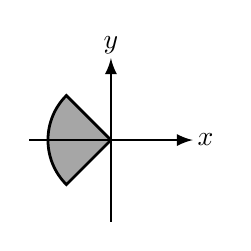
\begin{tikzpicture}[scale=.8]
            \begin{scope}
            \pgfsetlinewidth{1pt}
            \draw[fill=gray!70] (0,0) -- (135:1cm) arc (135:225:1cm) -- (0,0);
            \node at (0,1.5) {$y$};
            \node at (1.5,0) {$x$};
            \pgfsetarrowsend{latex}
            \draw (-1.3,0) to[->] (1.3,0);
            \draw (0,-1.3) to[->] (0,1.3);
            \end{scope}
            \end{tikzpicture}
            \begin{QOPS}
                \QOP 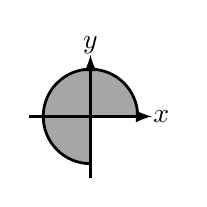
\begin{tikzpicture}[scale=.6]
                    \begin{scope}
                    \pgfsetlinewidth{1pt}
                    \draw[fill=gray!70] (0,0) -- (0:1cm) arc (0:270:1cm) -- (0,0);
                    \node at (0,1.5) {$y$};
                    \node at (1.5,0) {$x$};
                    \pgfsetarrowsend{latex}
                    \draw (-1.3,0) to[->] (1.3,0);
                    \draw (0,-1.3) to[->] (0,1.3);
                    \end{scope}
                    \end{tikzpicture}
                
                \QOP 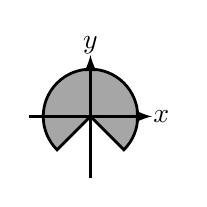
\begin{tikzpicture}[scale=.6]
                    \begin{scope}
                    \pgfsetlinewidth{1pt}
                    \draw[fill=gray!70] (0,0) -- (-45:1cm) arc (-45:225:1cm) -- (0,0);
                    \node at (0,1.5) {$y$};
                    \node at (1.5,0) {$x$};
                    \pgfsetarrowsend{latex}
                    \draw (-1.3,0) to[->] (1.3,0);
                    \draw (0,-1.3) to[->] (0,1.3);
                    \end{scope}
                    \end{tikzpicture}
                    
                \QOP 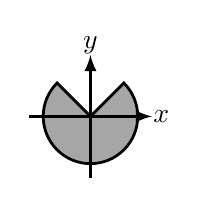
\begin{tikzpicture}[scale=.6]
                    \begin{scope}
                    \pgfsetlinewidth{1pt}
                    \draw[fill=gray!70] (0,0) -- (135:1cm) arc (-225:45:1cm) -- (0,0);
                    \node at (0,1.5) {$y$};
                    \node at (1.5,0) {$x$};
                    \pgfsetarrowsend{latex}
                    \draw (-1.3,0) to[->] (1.3,0);
                    \draw (0,-1.3) to[->] (0,1.3);
                    \end{scope}
                    \end{tikzpicture}
                \QOP 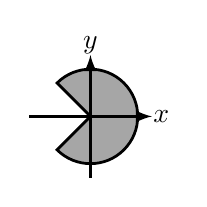
\begin{tikzpicture}[scale=.6]
                \begin{scope}
                \pgfsetlinewidth{1pt}
                \draw[fill=gray!70] (0,0) -- (225:1cm) arc (-135:135:1cm) -- (0,0);
                \node at (0,1.5) {$y$};
                \node at (1.5,0) {$x$};
                \pgfsetarrowsend{latex}
                \draw (-1.3,0) to[->] (1.3,0);
                \draw (0,-1.3) to[->] (0,1.3);
                \end{scope}
                \end{tikzpicture}
                
                \QOP 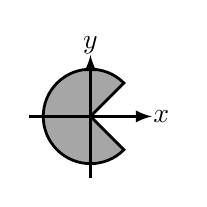
\begin{tikzpicture}[scale=.6]
                    \begin{scope}
                    \pgfsetlinewidth{1pt}
                    \draw[fill=gray!70] (0,0) -- (45:1cm) arc (45:315:1cm) -- (0,0);
                    \node at (0,1.5) {$y$};
                    \node at (1.5,0) {$x$};
                    \pgfsetarrowsend{latex}
                    \draw (-1.3,0) to[->] (1.3,0);
                    \draw (0,-1.3) to[->] (0,1.3);
                    \end{scope}
                    \end{tikzpicture}
            \end{QOPS}
        \end{QBODY}
        \begin{QFROMS}
        \end{QFROMS}
        \begin{QTAGS}\QTAG{B5C2三角函數II}\end{QTAGS}
        \begin{QANS}
            (5)
        \end{QANS}
        \begin{QSOLLIST}
        \end{QSOLLIST}
        \begin{QEMPTYSPACE}
        \end{QEMPTYSPACE}
    \end{QUESTION}
    \begin{QUESTION}
        \begin{ExamInfo}{93}{學測}{單選}{4}
        \end{ExamInfo}
        \begin{ExamAnsRateInfo}{23}{42}{17}{10}
        \end{ExamAnsRateInfo}
        \begin{QBODY}
            在坐標空間中給定兩點 $A(1,2,3)$ 與 $B(7,6,5)$。令 $S$ 為 $xy$- 平面上所有使得向量 $PA$ 垂直於向量 $PB$ 的 $P$ 點所成的集合,則
            \begin{QOPS} 
                \QOP $S$ 為空集合 
                \QOP $S$ 恰含一點 
                \QOP $S$ 恰含兩點 
                \QOP $S$ 為一線段 
                \QOP $S$ 為一圓
            \end{QOPS}
        \end{QBODY}
        \begin{QFROMS}
        \end{QFROMS}
        \begin{QTAGS}\QTAG{B4C1空間向量}\end{QTAGS}
        \begin{QANS}
            (1)
        \end{QANS}
        \begin{QSOLLIST}
        \end{QSOLLIST}
        \begin{QEMPTYSPACE}
        \end{QEMPTYSPACE}
    \end{QUESTION}
    \begin{QUESTION}
        \begin{ExamInfo}{93}{學測}{單選}{5}
        \end{ExamInfo}
        \begin{ExamAnsRateInfo}{61}{88}{62}{33}
        \end{ExamAnsRateInfo}
        \begin{QBODY}
            設 $\triangle ABC$ 為平面上的一個三角形,$P$ 為平面上一點且 $\lvec{AP}= \frac{1}{3}\lvec{AB}+ t\lvec{AC}$,其中 $t$為一實數。
            試問下列哪一選項為 $t$ 的最大範圍,使得 $P$ 落在 $\triangle ABC$ 的內部? 
            \begin{QOPS} 
                \QOP $0<t < \frac{1}{4}$ 
                \QOP $0 < t < \frac{1}{3}$ 
                \QOP $0 < t <\frac{1}{2}$ 
                \QOP $0 < t < \frac{2}{3}$ 
                \QOP $0 < t < \frac{3}{4}$
            \end{QOPS}
        \end{QBODY}
        \begin{QFROMS}
        \end{QFROMS}
        \begin{QTAGS}\QTAG{線性組合}\QTAG{B3C3-1平面向量的表示法}\QTAG{B3C3平面向量}\end{QTAGS}
        \begin{QANS}
            (4)
        \end{QANS}
        \begin{QSOLLIST}
        \end{QSOLLIST}
        \begin{QEMPTYSPACE}
        \end{QEMPTYSPACE}
    \end{QUESTION}
    \begin{QUESTION}
        \begin{ExamInfo}{93}{學測}{單選}{6}
        \end{ExamInfo}
        \begin{ExamAnsRateInfo}{26}{42}{27}{9}
        \end{ExamAnsRateInfo}
        \begin{QBODY}
            台灣證劵交易市場規定股票成交價格只能在前一個交易日的收盤價的漲、跌 $7\%$ 範圍內變動。例如:某支股票前一個交易日的收盤價是每股 100 元,則今天該支股票每股的買賣價格必須在 93 元至 107 元之間。假設有某支股票的價格起伏很大,某一天的收盤價是每股 40 元,次日起連續五個交易日以跌停板收盤 (每天跌 $7\%$),緊接著卻連續五個交易日以漲停板收盤(每天漲 $7\%$)。請問經過這十個交易日後,該支股票每股的收盤價最接近下列哪一個選項中的價格?
            \begin{QOPS}
                \QOP $39$ 元
                \QOP $39.5$ 元
                \QOP $40$ 元
                \QOP $40.5$ 元
                \QOP $41$ 元
            \end{QOPS}
        \end{QBODY}
        \begin{QFROMS}
        \end{QFROMS}
        \begin{QTAGS}\QTAG{應用問題}\QTAG{B1C3指對數函數}\QTAG{B1C3-5指數與對數的應用}\end{QTAGS}
        \begin{QANS}
            (1)
        \end{QANS}
        \begin{QSOLLIST}
        \end{QSOLLIST}
        \begin{QEMPTYSPACE}
        \end{QEMPTYSPACE}
    \end{QUESTION}
    \begin{QUESTION}
        \begin{ExamInfo}{93}{學測}{多選}{7}
        \end{ExamInfo}
        \begin{ExamAnsRateInfo}{56}{77}{61}{30}
        \end{ExamAnsRateInfo}
        \begin{QBODY}
            中山高速公路重慶北路交流道南下入口匝道分成內、外兩線車道,路旁立有標誌 「外側車道 大客車專用」。請選出不違反此規定的選項:
            \begin{QOPS}
                \QOP 小型車行駛內側車道 
                \QOP 小型車行駛外側車道 
                \QOP 大客車行駛內側車道 
                \QOP 大客車行駛外側車道 
                \QOP 大貨車行駛外側車道
            \end{QOPS}
        \end{QBODY}
        \begin{QFROMS}
        \end{QFROMS}
        \begin{QTAGS}\QTAG{邏輯}\QTAG{B2C2-1簡單的邏輯與集合}\QTAG{B2C2排列組合}\end{QTAGS}
        \begin{QANS}
            (1)(3)(4)
        \end{QANS}
        \begin{QSOLLIST}
        \end{QSOLLIST}
        \begin{QEMPTYSPACE}
        \end{QEMPTYSPACE}
    \end{QUESTION}
    \begin{QUESTION}
        \begin{ExamInfo}{93}{學測}{多選}{8}
        \end{ExamInfo}
        \begin{ExamAnsRateInfo}{43}{77}{39}{13}
        \end{ExamAnsRateInfo}
        \begin{QBODY}
            在坐標平面上,下列哪些方程式的圖形可以放進一個夠大的圓裡面? 
            \begin{QOPS} 
                \QOP $3x=2y^2$ 
                \QOP $3x^2+2y^2=1$ 
                \QOP $3x^2-2y^2=1$ \QOP $|x+y|=1$ 
                \QOP $|x|+|y|=1$
            \end{QOPS}
        \end{QBODY}
        \begin{QFROMS}
        \end{QFROMS}
        \begin{QTAGS}\QTAG{跨章節試題}\end{QTAGS}
        \begin{QANS}
            (2)(5)
        \end{QANS}
        \begin{QSOLLIST}
        \end{QSOLLIST}
        \begin{QEMPTYSPACE}
        \end{QEMPTYSPACE}
    \end{QUESTION}
    \begin{QUESTION}
        \begin{ExamInfo}{93}{學測}{多選}{9}
        \end{ExamInfo}
        \begin{ExamAnsRateInfo}{46}{70}{38}{30}
        \end{ExamAnsRateInfo}
        \begin{QBODY}
            如右圖 $O-ABCD$ 為一金字塔,底是邊長為 $1$ 之正方形,
            頂點 $O$ 與 $A$, $B$, $C$, $D$ 之距離均為 2。試問下列哪些式子是正確的?
            \begin{QOPS} 
                \QOP  $\lvec{OA}+\lvec{OB} +\lvec{OC}+\lvec{OD}=\lvec{0}$, 
                \QOP $\lvec{OA} + \lvec{OB}$  $-\lvec{OC}- \lvec{OD} =\lvec{0}$ 
                \QOP $\lvec{OA}- \lvec{OB}+ \lvec{OC} -\lvec{OD}= \lvec{0}$ 
                \QOP $\lvec{OA} \cdot \lvec{OB} = \lvec{OC} \cdot \lvec{OD}$
                \QOP $\lvec{OA}\cdot \lvec{OC}=2$。
            \end{QOPS}
            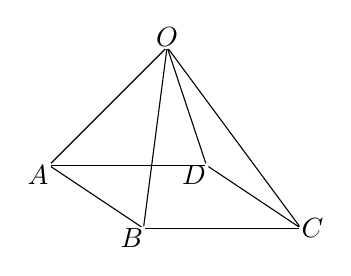
\begin{tikzpicture}[inner sep=0pt]
            \node (v00) at (0,0) {};
            \node[anchor =north east] (t00) at (v00) {$A$};
            \node (v01) at (1.2,-.8) {};
            \node[anchor =north east] (t01) at (v01) {$B$};
            \node (v10) at (2,0) {};
            \node[anchor = north east] (t10) at (v10) {$D$};
            \node (v11) at (3.2,-.8) {};
            \node[anchor =west] (t11) at (v11) {$C$};
            \node (vtop) at (1.5,1.5) {};
            \node[anchor =south] (ttop) at (vtop) {$O$};
            \draw (v00) to (v01);
            \draw (v00) to (v10);
            \draw (v11) to (v01);
            \draw (v11) to (v10);
            \draw (vtop) to (v01);
            \draw (vtop) to (v10);
            \draw (vtop) to (v11);
            \draw (vtop) to (v00);
            \end{tikzpicture}
        \end{QBODY}
        \begin{QFROMS}
        \end{QFROMS}
        \begin{QTAGS}\QTAG{B4C1-2空間向量的坐標表示法}\QTAG{B4C1空間向量}\end{QTAGS}
        \begin{QANS}
            (3)(4)
        \end{QANS}
        \begin{QSOLLIST}
        \end{QSOLLIST}
        \begin{QEMPTYSPACE}
        \end{QEMPTYSPACE}
    \end{QUESTION}
    \begin{QUESTION}
        \begin{ExamInfo}{93}{學測}{多選}{10}
        \end{ExamInfo}
        \begin{ExamAnsRateInfo}{43}{77}{40}{12}
        \end{ExamAnsRateInfo}
        \begin{QBODY}
            從 $1,2,\dots ,10$ 這十個數中隨意取兩個,以 $p$ 表示其和為偶數之機率, $q$ 表示其和為奇數之機率。 試問下列哪些敘述是正確的?
             \begin{QOPS} 
                \QOP $p+q=1$ 
                \QOP $p=q$  
                \QOP $|p-q| \leq \frac{1}{10} $ 
                \QOP $|p-q| \geq \frac{1}{20}$ \QOP $p\geq \frac{1}{2}$
            \end{QOPS}
        \end{QBODY}
        \begin{QFROMS}
        \end{QFROMS}
        \begin{QTAGS}\QTAG{B2C3機率}\QTAG{B2C3-2機率的定義與性質}\end{QTAGS}
        \begin{QANS}
            (1)(4)
        \end{QANS}
        \begin{QSOLLIST}
        \end{QSOLLIST}
        \begin{QEMPTYSPACE}
        \end{QEMPTYSPACE}
    \end{QUESTION}
    \begin{QUESTION}
        \begin{ExamInfo}{93}{學測}{多選}{11}
        \end{ExamInfo}
        \begin{ExamAnsRateInfo}{29}{55}{23}{9}
        \end{ExamAnsRateInfo}
        \begin{QBODY}
            設 $f(x)$ 為三次實係數多項式,且知複數 $1+i$ 為 $f(x)=0$ 之一解,
            試問下列哪些敘述是正確的?
            \begin{QOPS} 
                \QOP $f(1-i)=0$ \quad 
                \QOP $f(2+i) \neq 0$ 
                \QOP 沒有實數解 $x$ 滿足 $f(x)=x$ 
                \QOP 沒有實數解 $x$ 滿足 $f(x^3)=x$ 
                \QOP 若 $f(0)>0$ 且 $f(2) <0$,則 $f(4)<0$ 
            \end{QOPS}
        \end{QBODY}
        \begin{QFROMS}
        \end{QFROMS}
        \begin{QTAGS}\QTAG{B1C2多項式函數}\QTAG{B1C2-3多項式方程式}\QTAG{勘根定理}\QTAG{虛根定理}\QTAG{複數}\end{QTAGS}
        \begin{QANS}
            (1)(2)(5)
        \end{QANS}
        \begin{QSOLLIST}
        \end{QSOLLIST}
        \begin{QEMPTYSPACE}
        \end{QEMPTYSPACE}
    \end{QUESTION}
    \begin{QUESTION}
        \begin{ExamInfo}{93}{學測}{填充}{A}
        \end{ExamInfo}
        \begin{ExamAnsRateInfo}{70}{90}{77}{43}
        \end{ExamAnsRateInfo}
        \begin{QBODY}
            某數學老師計算學期成績的公式如下:五次平時考中取較好的三次之平均值佔 $30\%$,兩次期中考各佔 $20\%$,期末考佔 $30\%$。某生平時考成績分別為 68、82、70、73、85,期中考成績分別為 86、79,期末考成績為 90,則該生學期成績為 
            \TCNBOX{\TCN\TCN}。(計算到整數為止,小數點以後四捨五入)
        \end{QBODY}
        \begin{QFROMS}
        \end{QFROMS}
        \begin{QTAGS}\QTAG{B2C4-1一維數據分析}\QTAG{B2C4數據分析}\QTAG{加權平均數}\end{QTAGS}
        \begin{QANS}
            $84$
        \end{QANS}
        \begin{QSOLLIST}
        \end{QSOLLIST}
        \begin{QEMPTYSPACE}
        \end{QEMPTYSPACE}
    \end{QUESTION}
    \begin{QUESTION}
        \begin{ExamInfo}{93}{學測}{填充}{B}
        \end{ExamInfo}
        \begin{ExamAnsRateInfo}{25}{57}{16}{2}
        \end{ExamAnsRateInfo}
        \begin{QBODY}
            某電視台舉辦抽獎遊戲,現場準備的抽獎箱裡放置了四個分別標有 1000、 800、 600、 0 元獎額的球。
            參加者自行從抽獎箱裡摸取一球(取後即放回),
            主辦單位即贈送與此球上數字等額的獎金,並規定抽取到 0 元的人可以再摸一次,但是所得獎金折半(若再摸到 0 就沒有第三次機會);則一個參加者可得獎金的期望值是 
            \TCNBOX{\TCN\TCN\TCN} 元。(計算到整數為止,小數點以後四捨五入)
        \end{QBODY}
        \begin{QFROMS}
        \end{QFROMS}
        \begin{QTAGS}\QTAG{B5C1機率與統計}\end{QTAGS}
        \begin{QANS}
            $675$
        \end{QANS}
        \begin{QSOLLIST}
        \end{QSOLLIST}
        \begin{QEMPTYSPACE}
        \end{QEMPTYSPACE}
    \end{QUESTION}
    \begin{QUESTION}
        \begin{ExamInfo}{93}{學測}{填充}{C}
        \end{ExamInfo}
        \begin{ExamAnsRateInfo}{36}{77}{27}{4}
        \end{ExamAnsRateInfo}
        \begin{QBODY}
            設 $a,b,c$ 為正整數,若 $a\log_{520} 2+b\log_{520} 5+c\log_{520}13=3$,則 $a+b+c=$ 
            \TCNBOX{} 。
        \end{QBODY}
        \begin{QFROMS}
        \end{QFROMS}
        \begin{QTAGS}\QTAG{B1C3-3對數}\QTAG{B1C3指對數函數}\QTAG{對數律}\end{QTAGS}
        \begin{QANS}
            $15$
        \end{QANS}
        \begin{QSOLLIST}
        \end{QSOLLIST}
        \begin{QEMPTYSPACE}
        \end{QEMPTYSPACE}
    \end{QUESTION}
    \begin{QUESTION}
        \begin{ExamInfo}{93}{學測}{填充}{D}
        \end{ExamInfo}
        \begin{ExamAnsRateInfo}{19}{45}{8}{4}
        \end{ExamAnsRateInfo}
        \begin{QBODY}
            設 $\triangle ABC$ 為一等腰直角三角形,$\angle BAC = 90^\circ$ 。
            若 $P$, $Q$ 為斜邊 $\overline{BC}$ 的三等分點,則 $\tan \angle PAQ = $
            \TCNBOX{\TCN\TCN} 。
        \end{QBODY}
        \begin{QFROMS}
        \end{QFROMS}
        \begin{QTAGS}\QTAG{B3C3-2平面向量的內積}\QTAG{B3C3平面向量}\QTAG{夾角}\end{QTAGS}
        \begin{QANS}
            $\frac{3}{4}$
        \end{QANS}
        \begin{QSOLLIST}
        \end{QSOLLIST}
        \begin{QEMPTYSPACE}
        \end{QEMPTYSPACE}
    \end{QUESTION}
    \begin{QUESTION}
        \begin{ExamInfo}{93}{學測}{填充}{E}
        \end{ExamInfo}
        \begin{ExamAnsRateInfo}{52}{77}{56}{23}
        \end{ExamAnsRateInfo}
        \begin{QBODY}
            某高中招收高一新生共有男生 1008 人、女生 924 人報到。學校想將他們依男女合班的原則平均分班,且要求各班有同樣多的男生,也有同樣多的女生;考量教學效益,並限制各班總人數在 40 與 50 人之間,則共分成	
            \TCNBOX{\TCN\TCN} 班。
        \end{QBODY}
        \begin{QFROMS}
        \end{QFROMS}
        \begin{QTAGS}\QTAG{不是99課綱}\end{QTAGS}
        \begin{QANS}
            $42$
        \end{QANS}
        \begin{QSOLLIST}
        \end{QSOLLIST}
        \begin{QEMPTYSPACE}
        \end{QEMPTYSPACE}
    \end{QUESTION}
    \begin{QUESTION}
        \begin{ExamInfo}{93}{學測}{填充}{F}
        \end{ExamInfo}
        \begin{ExamAnsRateInfo}{26}{61}{15}{2}
        \end{ExamAnsRateInfo}
        \begin{QBODY}
            在坐標空間中,平面 $x-2y+z=0$ 上有一以點 $P(1,1,1)$ 為圓心的圓 $\Gamma$ ,
            而 $Q(-9,9, 27)$ 為圓 $\Gamma$ 上 一點。
            若過 $Q$ 與圓  $\Gamma$ 相切的直線之一方向向量為 $(a, b, 1)$,則 $a= 
            \TCNBOX{\TCN}$, $b= 
            \TCNBOX{\TCN}$。
        \end{QBODY}
        \begin{QFROMS}
        \end{QFROMS}
        \begin{QTAGS}\QTAG{B4C2空間中的平面與直線}\QTAG{B4C2-1平面方程式}\end{QTAGS}
        \begin{QANS}
            $a=5, b=3$
        \end{QANS}
        \begin{QSOLLIST}
        \end{QSOLLIST}
        \begin{QEMPTYSPACE}
        \end{QEMPTYSPACE}
    \end{QUESTION}
    \begin{QUESTION}
        \begin{ExamInfo}{93}{學測}{填充}{G}
        \end{ExamInfo}
        \begin{ExamAnsRateInfo}{10}{27}{3}{0}
        \end{ExamAnsRateInfo}
        \begin{QBODY}
            設 $270^\circ <A< 360^\circ$ 且 $\sqrt{3}\sin A+ \cos A=2 \sin {2004} ^\circ$。若 $A=m^\circ$,則 $m=$
            \TCNBOX{\TCN\TCN\TCN}。
        \end{QBODY}
        \begin{QFROMS}
        \end{QFROMS}
        \begin{QTAGS}\QTAG{B5C2三角函數II}\QTAG{B5C2-2三角函數的應用}\end{QTAGS}
        \begin{QANS}
            $306$
        \end{QANS}
        \begin{QSOLLIST}
        \end{QSOLLIST}
        \begin{QEMPTYSPACE}
        \end{QEMPTYSPACE}
    \end{QUESTION}
    \begin{QUESTION}
        \begin{ExamInfo}{93}{學測}{填充}{H}
        \end{ExamInfo}
        \begin{ExamAnsRateInfo}{21}{37}{18}{8}
        \end{ExamAnsRateInfo}
        \begin{QBODY}
            坐標平面上的圓 $C:(x-7)^2+(y-8)^2=9$ 上有 
            \TCNBOX{\TCN\TCN} 個點與原點的距離正好是整數值。
        \end{QBODY}
        \begin{QFROMS}
        \end{QFROMS}
        \begin{QTAGS}\QTAG{B3C2-3圓與直線的關係}\QTAG{圖形}\QTAG{B3C2直線與圓}\end{QTAGS}
        \begin{QANS}
            $12$
        \end{QANS}
        \begin{QSOLLIST}
        \end{QSOLLIST}
        \begin{QEMPTYSPACE}
        \end{QEMPTYSPACE}
    \end{QUESTION}
    \begin{QUESTION}
        \begin{ExamInfo}{93}{學測}{填充}{I}
        \end{ExamInfo}
        \begin{ExamAnsRateInfo}{19}{47}{7}{3}
        \end{ExamAnsRateInfo}
        \begin{QBODY}
            在坐標平面上,設直線 $L:y=x+2$ 與拋物線 $\Gamma :x^2=4y$ 相交於 $P,Q$ 兩點。若 $F$ 表拋物線 $\Gamma$ 的焦點,則 $\overline{PF}+\overline{QF}=$ 
            $\TCNBOX{\TCN\TCN}$
        \end{QBODY}
        \begin{QFROMS}
        \end{QFROMS}
        \begin{QTAGS}\QTAG{B4C4二次曲線}\QTAG{B4C4-1拋物線}\QTAG{圖形}\end{QTAGS}
        \begin{QANS}
            $10$
        \end{QANS}
        \begin{QSOLLIST}
        \end{QSOLLIST}
        \begin{QEMPTYSPACE}
        \end{QEMPTYSPACE}
    \end{QUESTION}

% !TEX encoding = UTF-8 Unicode
% !TEX TS-program = xelatex
\begin{QUESTIONS}
    \begin{QUESTION}
        \begin{ExamInfo}{94}{學測}{單選}{1}
        \end{ExamInfo}
        \begin{ExamAnsRateInfo}{73}{91}{78}{50}
        \end{ExamAnsRateInfo}
        \begin{QBODY}
            試問整數 43659 共有多少個不同的質因數? 
			\begin{QOPS} 
				\QOP 1 個 
				\QOP 2 個 
				\QOP 3 個 
				\QOP 4 個 
				\QOP 5 個
			\end{QOPS}
        \end{QBODY}
        \begin{QFROMS}
        \end{QFROMS}
        \begin{QTAGS}\QTAG{不是99課綱}\end{QTAGS}
        \begin{QANS}
            (3)
        \end{QANS}
        \begin{QSOLLIST}
        \end{QSOLLIST}
        \begin{QEMPTYSPACE}
        \end{QEMPTYSPACE}
    \end{QUESTION}
    \begin{QUESTION}
        \begin{ExamInfo}{94}{學測}{單選}{2}
        \end{ExamInfo}
        \begin{ExamAnsRateInfo}{78}{98}{89}{47}
        \end{ExamAnsRateInfo}
        \begin{QBODY}
            利用公式 $1^3 +2^3 + \cdots +n^3 = (\frac{n(n+1)}{2})^2$,可計算出 $(11)^3 + (12)^3 + \cdots +(20)^3$ 之值為 
		\begin{QOPS} 
			\QOP 41075
			\QOP 41095
			\QOP 41115	
			\QOP 41135	
			\QOP 41155
		\end{QOPS}
        \end{QBODY}
        \begin{QFROMS}
        \end{QFROMS}
        \begin{QTAGS}\QTAG{B2C1數列級數}\QTAG{B2C1-2級數}\end{QTAGS}
        \begin{QANS}
            (1)
        \end{QANS}
        \begin{QSOLLIST}
        \end{QSOLLIST}
        \begin{QEMPTYSPACE}
        \end{QEMPTYSPACE}
    \end{QUESTION}
    \begin{QUESTION}
        \begin{ExamInfo}{94}{學測}{單選}{3}
        \end{ExamInfo}
        \begin{ExamAnsRateInfo}{52}{82}{54}{20}
        \end{ExamAnsRateInfo}
        \begin{QBODY}
            台北銀行最早發行的樂透彩(俗稱小樂透)的玩法是「42 選 6」:購買者從 01 $\sim$ 42 中任選六個 號碼,當這六個號碼與開出的六個號碼完全相同(不計次序)時即得頭獎;台北銀行曾考慮改發行「39 選 5」的小小樂透:購買者從 01 $\sim$ 39 中任選五個號碼,如果這五個號碼與開出的五個號碼完全相同(不計次序)則得頭獎。假設原來的小樂透中頭獎的機率是 $R$,而曾考慮發行的小小樂透中頭獎的機率是 $r$。試問比值 $\frac{r}{R}$ 最接近下列哪個選項?
			\begin{QOPS}
				\QOP $3$
				\QOP $5$
				\QOP $7$
				\QOP $9$
				\QOP $11$
			\end{QOPS}
        \end{QBODY}
        \begin{QFROMS}
        \end{QFROMS}
        \begin{QTAGS}\QTAG{B2C3機率}\QTAG{B2C3-2機率的定義與性質}\end{QTAGS}
        \begin{QANS}
            (4)
        \end{QANS}
        \begin{QSOLLIST}
        \end{QSOLLIST}
        \begin{QEMPTYSPACE}
        \end{QEMPTYSPACE}
    \end{QUESTION}
    \begin{QUESTION}
        \begin{ExamInfo}{94}{學測}{單選}{4}
        \end{ExamInfo}
        \begin{ExamAnsRateInfo}{32}{65}{21}{10}
        \end{ExamAnsRateInfo}
        \begin{QBODY}
            設 $a, b$ 為正實數,已知 $\log_7 a = 11$,$\log_7 b = 13$ ;試問 $\log_7 (a + b)$ 之值最接近下列哪個選項? 
			\begin{QOPS} 
				\QOP 12 
				\QOP 13 
				\QOP 14 
				\QOP 23 
				\QOP 24
			\end{QOPS}
        \end{QBODY}
        \begin{QFROMS}
        \end{QFROMS}
        \begin{QTAGS}\QTAG{B1C3-3對數}\QTAG{B1C3指對數函數}\QTAG{對數律}\end{QTAGS}
        \begin{QANS}
            (2)
        \end{QANS}
        \begin{QSOLLIST}
        \end{QSOLLIST}
        \begin{QEMPTYSPACE}
        \end{QEMPTYSPACE}
    \end{QUESTION}
    \begin{QUESTION}
        \begin{ExamInfo}{94}{學測}{單選}{5}
        \end{ExamInfo}
        \begin{ExamAnsRateInfo}{8}{10}{7}{7}
        \end{ExamAnsRateInfo}
        \begin{QBODY}
            某校高一第一次段考數學成績不太理想,多數同學成績偏低;考慮到可能是同學們適應不良所致,數學老師決定將每人的原始成績取平方根後再乘以 10 作為正式紀錄的成績。今隨機抽選 100 位同學,發現調整後的成績其平均為 65 分,標準差為 15 分;試問這 100 位同學未調整前的成績之平均 $M$ 介於哪兩個連續正整數之間? 
			\begin{QOPS} 
				\QOP $40 \leq M <41$ 
				\QOP $41\leq  M<42$ 
				\QOP$ 42 \leq M<43$        
				\QOP $43 \leq M<44$        
				\QOP $44\leq  M<45$
			\end{QOPS}
        \end{QBODY}
        \begin{QFROMS}
        \end{QFROMS}
        \begin{QTAGS}\QTAG{平均數}\QTAG{B2C4-1一維數據分析}\QTAG{B2C4數據分析}\QTAG{標準差}\end{QTAGS}
        \begin{QANS}
            (5)
        \end{QANS}
        \begin{QSOLLIST}
        \end{QSOLLIST}
        \begin{QEMPTYSPACE}
        \end{QEMPTYSPACE}
    \end{QUESTION}
\end{QUESTIONS}
\begin{QUESTIONS}
    \begin{QUESTION}
        \begin{ExamInfo}{94}{學測}{多選}{6}
        \end{ExamInfo}
        \begin{ExamAnsRateInfo}{53}{81}{52}{26}
        \end{ExamAnsRateInfo}
        \begin{QBODY}
            如右圖所示,兩射線 $\lvec{OA}$ 與 $\lvec{OB}$ 交於 $O$ 點,試問下列選項中哪些向量的終點會落在陰影區域內?
			\begin{QOPS} 
				\QOP $\lvec{OA} + 2\lvec{OB}$
				\QOP  $\frac{3}{4}\lvec{OA} + \frac{1}{3} \lvec{OB}$ 
				\QOP $\frac{3}{4}\lvec{OA} - \frac{1}{3}\lvec{OB}$ 
				\QOP $\frac{3}{4}\lvec{OA} + \frac{1}{5} \lvec{OB}$ 
				\QOP $\frac{3}{4}\lvec{OA} - \frac{1}{5} \lvec{OB}$
			\end{QOPS}
			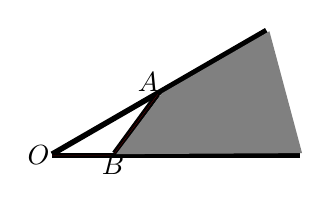
\begin{tikzpicture}[scale=.8]
				\begin{scope}[inner sep=0pt]
				\node (vO) at (0,0) {};
				\node[anchor = east] (tO) at (vO) {$O$};
				\node (vB) at (0:1) {};
				\node[anchor = north] (tB) at (vB) {$B$};
				\node (vD) at (0:4) {};
				\node (vA) at (30:2) {};
				\node[anchor = south  east] (tA) at (vA) {$A$};
				\node (vC) at (30:4) {};
				\draw[line width=2pt] (vA) to (vB);
				\draw[line width=2pt] (vO) to (vD);
				\draw[line width=2pt] (vO) to (vC);
				\fill[red] (vA) -- (vB) -- (vO);
				\fill[gray]  (1:1.05) -- (.5:4) -- (29.5:4) -- (29:2.03);
				\end{scope}
			\end{tikzpicture}
        \end{QBODY}
        \begin{QFROMS}
        \end{QFROMS}
        \begin{QTAGS}\QTAG{線性組合}\QTAG{B3C3-1平面向量的表示法}\QTAG{B3C3平面向量}\end{QTAGS}
        \begin{QANS}
            (1)(2)
        \end{QANS}
        \begin{QSOLLIST}
        \end{QSOLLIST}
        \begin{QEMPTYSPACE}
        \end{QEMPTYSPACE}
    \end{QUESTION}
    \begin{QUESTION}
        \begin{ExamInfo}{94}{學測}{多選}{7}
        \end{ExamInfo}
        \begin{ExamAnsRateInfo}{56}{87}{59}{22}
        \end{ExamAnsRateInfo}
        \begin{QBODY}
            如右圖所示,坐標平面上一鳶形 $ABCD$, 其中 $A,C$ 在 $y$-軸上, $B$, $D$ 在 $x$-軸上, 且 $\overline{AB} = \overline{AD} =2$, $\overline{BC} = \overline{CD} =4$, $\overline{AC} =5$。 令 $m_{AB}$, $m_{BC}$, $m_{CD}$,  $m_{DA}$ 分別表直線 $AB$, $BC$, $CD$, $DA$ 之斜率。試問以下哪些敘述成立? 
			\begin{QOPS} 
				\QOP 此四數值中以 $m_{AB}$ 為最大 
				\QOP 此四數值中以 $m_{BC}$ 為最小 
				\QOP $m_{BC}= - m_{CD}$  
				\QOP $m_{AB} \times m_{BC} =-1$ 
				\QOP $m_{CD} +m_{DA} >0$
			\end{QOPS}
			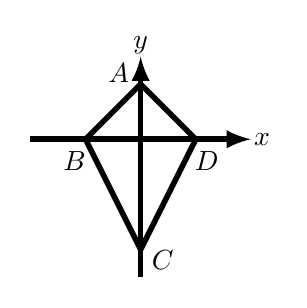
\begin{tikzpicture}[scale=.7]
				\pgfsetlinewidth{2pt}
				\node at (0,1.7) {$y$};
				\node at (2.2,0) {$x$};
				\node at (1.2,-.4) {$D$};
				\node at (-1.2,-.4) {$B$};
				\node at (-.4,1.2) {$A$};
				\node at (.4,-2.2) {$C$};
				\draw (1,0) to (0,1);
				\draw (-1,0) to (0,1);
				\draw (1,0) to (0,-2);
				\draw (-1,0) to (0,-2);
				\pgfsetarrowsend{latex}
				\draw (-2,0) to[->] (2,0);
				\draw (0,-2.5) to[->] (0,1.5);
			\end{tikzpicture}
        \end{QBODY}
        \begin{QFROMS}
        \end{QFROMS}
        \begin{QTAGS}\QTAG{B3C2-1直線方程式及其圖形}\QTAG{B3C2直線與圓}\end{QTAGS}
        \begin{QANS}
            (2)(3)(5)
        \end{QANS}
        \begin{QSOLLIST}
        \end{QSOLLIST}
        \begin{QEMPTYSPACE}
        \end{QEMPTYSPACE}
    \end{QUESTION}
    \begin{QUESTION}
        \begin{ExamInfo}{94}{學測}{多選}{8}
        \end{ExamInfo}
        \begin{ExamAnsRateInfo}{34}{67}{22}{13}
        \end{ExamAnsRateInfo}
        \begin{QBODY}
            假設坐標空間中三相異平面 $E_1$, $E_2$, $E_3$ 皆通過 $(-1,2,0)$ 與 $(3,0,2)$ 兩點,試問以下哪些點也同時在此三平面上? 
			\begin{QOPS} 
				\QOP (2,2,2) 
				\QOP (1,1,1) 
				\QOP (4,-2,2) 
				\QOP (-2,4,0) 
				\QOP (-5,-4,-2)
			\end{QOPS}
        \end{QBODY}
        \begin{QFROMS}
        \end{QFROMS}
        \begin{QTAGS}\QTAG{B4C2空間中的平面與直線}\QTAG{B4C2-2空間直線方程式}\end{QTAGS}
        \begin{QANS}
            (2)
        \end{QANS}
        \begin{QSOLLIST}
        \end{QSOLLIST}
        \begin{QEMPTYSPACE}
        \end{QEMPTYSPACE}
    \end{QUESTION}
    \begin{QUESTION}
        \begin{ExamInfo}{94}{學測}{多選}{9}
        \end{ExamInfo}
        \begin{ExamAnsRateInfo}{37}{69}{32}{10}
        \end{ExamAnsRateInfo}
        \begin{QBODY}
            若 $0 < \theta < \frac{\pi}{4}$ ,試問以下哪些選項恆成立? 
			\begin{QOPS} 
				\QOP	$\sin \theta < \cos \theta$	
				\QOP	$\tan \theta < \sin \theta$ 
				\QOP $\cos \theta < \tan \theta$ 
				\QOP $\sin{2\theta} <\cos{2\theta}$ 
				\QOP $\tan{\frac{\theta}{2}} <\frac{1}{2} \tan \theta$
			\end{QOPS}
        \end{QBODY}
        \begin{QFROMS}
        \end{QFROMS}
        \begin{QTAGS}\QTAG{B3C1-1簡單的三角函數}\QTAG{B3C1三角}\end{QTAGS}
        \begin{QANS}
            (1)(5)
        \end{QANS}
        \begin{QSOLLIST}
        \end{QSOLLIST}
        \begin{QEMPTYSPACE}
        \end{QEMPTYSPACE}
    \end{QUESTION}
    \begin{QUESTION}
        \begin{ExamInfo}{94}{學測}{多選}{10}
        \end{ExamInfo}
        \begin{ExamAnsRateInfo}{29}{47}{23}{17}
        \end{ExamAnsRateInfo}
        \begin{QBODY}
            設 $F_1$ 與 $F_2$ 為坐標平面上雙曲線 $\Gamma : \frac{x^2}{9} -\frac{y^2}{16} =1$ 的兩個焦點,$P$ 為 $\Gamma$ 上一點,使得此三點構成一等腰三角形。試問以下哪些值可能是這些等腰三角形的週長? 
			\begin{QOPS} 
				\QOP 20	
				\QOP 24 
				\QOP 28 
				\QOP 32	
				\QOP 36 。
			\end{QOPS}
        \end{QBODY}
        \begin{QFROMS}
        \end{QFROMS}
        \begin{QTAGS}\QTAG{B4C4-3雙曲線}\QTAG{B4C4二次曲線}\QTAG{圖形}\end{QTAGS}
        \begin{QANS}
            (2)(5)
        \end{QANS}
        \begin{QSOLLIST}
        \end{QSOLLIST}
        \begin{QEMPTYSPACE}
        \end{QEMPTYSPACE}
    \end{QUESTION}
    \begin{QUESTION}
        \begin{ExamInfo}{94}{學測}{多選}{11}
        \end{ExamInfo}
        \begin{ExamAnsRateInfo}{32}{51}{30}{15}
        \end{ExamAnsRateInfo}
        \begin{QBODY}
            設 $S$ 為空間中一球面, $\overline{AB}$ 為其一直徑,且 $\overline{AB} =10$。若 $ P$ 為空間中一點,使得 $\overline{PA} + \overline{PB} = 14$, 則 $P$ 點的位置可能落在哪裡? 
			\begin{QOPS} 
				\QOP 線段 $\overline{AB}$ 上; 
				\QOP 直線 $AB$ 上,但不在線段 $\overline{AB}$ 上; 
				\QOP	球面 $S$ 上; 
				\QOP 球 $S$ 的內部,但不在線段 $AB$ 上; 
				\QOP 球 $S$ 的外部,但不在直線 AB 上。
			\end{QOPS}
        \end{QBODY}
        \begin{QFROMS}
        \end{QFROMS}
        \begin{QTAGS}\QTAG{不是99課綱}\end{QTAGS}
        \begin{QANS}
            (2)(3)(4)(5)
        \end{QANS}
        \begin{QSOLLIST}
        \end{QSOLLIST}
        \begin{QEMPTYSPACE}
        \end{QEMPTYSPACE}
    \end{QUESTION}
\end{QUESTIONS}
\begin{QUESTIONS}
    \begin{QUESTION}
        \begin{ExamInfo}{94}{學測}{填充}{A}
        \end{ExamInfo}
        \begin{ExamAnsRateInfo}{69}{92}{82}{33}
        \end{ExamAnsRateInfo}
        \begin{QBODY}
            若多項式 $x^2 +x+2$ 能整除 $x^5 + x^4 +x^3 +px^2 +2x+q$,
			則 $p= \TCNBOX{\TCN}$、 $q=\TCNBOX{\TCN}$ 。
        \end{QBODY}
        \begin{QFROMS}
        \end{QFROMS}
        \begin{QTAGS}\QTAG{B1C2多項式函數}\QTAG{多項式除法}\QTAG{B1C2-2多項式的運算與應用}\end{QTAGS}
        \begin{QANS}
            $p=3,q=8$
        \end{QANS}
        \begin{QSOLLIST}
        \end{QSOLLIST}
        \begin{QEMPTYSPACE}
        \end{QEMPTYSPACE}
    \end{QUESTION}
    \begin{QUESTION}
        \begin{ExamInfo}{94}{學測}{填充}{B}
        \end{ExamInfo}
        \begin{ExamAnsRateInfo}{39}{78}{34}{5}
        \end{ExamAnsRateInfo}
        \begin{QBODY}
            在坐標平面上,正方形 $ABCD$ 的四個頂點坐標分別為 $A(0,1)$, $B(0,0)$, $C(1,0)$, $D(1,1)$。設 $P$ 為 正方形 $ABCD$ 內部的一點,若 $\triangle PDA$ 與 $\triangle PBC$ 的面積比為 $1:2$,且 $\triangle PAB$ 與 $\triangle PCD$ 的面積比為 $2:3$,則 $P$ 點的坐標為 $\TCNBOX{ (\FR{\TCN}{\TCN}, \FR{\TCN}{\TCN})}$。
        \end{QBODY}
        \begin{QFROMS}
        \end{QFROMS}
        \begin{QTAGS}\QTAG{面積}\QTAG{B3C3-3面積與二階行列式}\QTAG{B3C3-1平面向量的表示法}\QTAG{B3C3平面向量}\QTAG{線性組合}\end{QTAGS}
        \begin{QANS}
            $(\frac{2}{5},\frac{2}{3})$
        \end{QANS}
        \begin{QSOLLIST}
        \end{QSOLLIST}
        \begin{QEMPTYSPACE}
        \end{QEMPTYSPACE}
    \end{QUESTION}
    \begin{QUESTION}
        \begin{ExamInfo}{94}{學測}{填充}{C}
        \end{ExamInfo}
        \begin{ExamAnsRateInfo}{51}{80}{51}{22}
        \end{ExamAnsRateInfo}
        \begin{QBODY}
            在數線上有一個運動物體從原點出發,在此數線上跳動,每次向正方向或負方向跳 1 個單 位,跳動過程可重複經過任何一點。若經過 6 次跳動後運動物體落在點 $+4$ 處,則此運動物體共有 
			$\TCNBOX{\TCN}$ 種不同的跳動方法。
        \end{QBODY}
        \begin{QFROMS}
        \end{QFROMS}
        \begin{QTAGS}\QTAG{B2C2-2排列}\QTAG{含相同物排列}\QTAG{B2C2排列組合}\end{QTAGS}
        \begin{QANS}
            $6$
        \end{QANS}
        \begin{QSOLLIST}
        \end{QSOLLIST}
        \begin{QEMPTYSPACE}
        \end{QEMPTYSPACE}
    \end{QUESTION}
    \begin{QUESTION}
        \begin{ExamInfo}{94}{學測}{填充}{D}
        \end{ExamInfo}
        \begin{ExamAnsRateInfo}{21}{48}{14}{1}
        \end{ExamAnsRateInfo}
        \begin{QBODY}
            設複數 $z=1-i$;若 $1+z+z^2 + \cdots +z^9 =a+bi$,其中 $a$, $b$ 為實數,則$ a= \TCNBOX{\TCN\TCN}$ 、 $b=\TCNBOX{\TCN\TCN}$ 。
        \end{QBODY}
        \begin{QFROMS}
        \end{QFROMS}
        \begin{QTAGS}\QTAG{B2C1數列級數}\QTAG{複數}\QTAG{B2C1-2級數}\QTAG{B1C2多項式函數}\QTAG{B1C2-3多項式方程式}\QTAG{等比級數}\end{QTAGS}
        \begin{QANS}
            $32, -1$
        \end{QANS}
        \begin{QSOLLIST}
        \end{QSOLLIST}
        \begin{QEMPTYSPACE}
        \end{QEMPTYSPACE}
    \end{QUESTION}
    \begin{QUESTION}
        \begin{ExamInfo}{94}{學測}{填充}{E}
        \end{ExamInfo}
        \begin{ExamAnsRateInfo}{13}{36}{3}{0}
        \end{ExamAnsRateInfo}
        \begin{QBODY}
            設 $O$ 為坐標平面上的原點,$P$ 點坐標為 $(2, 1)$;若 $A$, $B$ 分別是正 $x$-軸及正 $y$-軸上的點,使得 $PA \bot PB$ ,則 $\triangle OAB$ 面積的最大可能值為 $\TCNBOX{\FR{\TCN\TCN}{\TCN\TCN}}$。
        \end{QBODY}
        \begin{QFROMS}
        \end{QFROMS}
        \begin{QTAGS}\QTAG{面積}\QTAG{B3C3-2平面向量的內積}\QTAG{B3C3平面向量}\QTAG{B3C3-3面積與二階行列式}\end{QTAGS}
        \begin{QANS}
            $\frac{25}{16}$
        \end{QANS}
        \begin{QSOLLIST}
        \end{QSOLLIST}
        \begin{QEMPTYSPACE}
        \end{QEMPTYSPACE}
    \end{QUESTION}
    \begin{QUESTION}
        \begin{ExamInfo}{94}{學測}{填充}{F}
        \end{ExamInfo}
        \begin{ExamAnsRateInfo}{17}{38}{8}{5}
        \end{ExamAnsRateInfo}
        \begin{QBODY}
            如右圖所示,在 $\triangle ABC$ 中, $\angle BAC$ 的平分線 $AD$ 交對邊 $BC$ 於$D$;已知 $\overline{BD}=3$, $\overline{DC} = 6$ 且 $\overline{AB} = \overline{AD}$ ,則 $\cos \angle BAD$ 之值為 $\TCNBOX{\FR{\TCN}{\TCN}}$ 。
			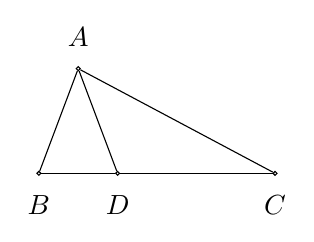
\begin{tikzpicture}[inner sep = 0pt]
				\tikzstyle{vnode}=[draw,circle,inner sep=.5pt];
				\node[vnode]  (vB) at (0,0) {};
				\node  (tB) at (0,-.4) {$B$};
				\node[vnode]  (vD) at (1,0) {};
				\node  (tD) at (1,-.4) {$D$};
				\node[vnode]  (vC) at (3,0) {};
				\node  (tC) at (3,-.4) {$C$};
				\node[vnode]  (vA) at (.5,1.33) {};
				\node  (tA) at (.5,1.73) {$A$}; 
				\draw (vB) to (vD);
				\draw (vC) to (vD);
				\draw (vA) to (vD);
				\draw (vB) to (vA);
				\draw (vC) to (vA);
			\end{tikzpicture}
        \end{QBODY}
        \begin{QFROMS}
        \end{QFROMS}
        \begin{QTAGS}\QTAG{B3C1-3正弦定理與餘弦定理}\QTAG{B3C1三角}\end{QTAGS}
        \begin{QANS}
            $\dfrac{3}{4}$
        \end{QANS}
        \begin{QSOLLIST}
        \end{QSOLLIST}
        \begin{QEMPTYSPACE}
        \end{QEMPTYSPACE}
    \end{QUESTION}
    \begin{QUESTION}
        \begin{ExamInfo}{94}{學測}{填充}{G}
        \end{ExamInfo}
        \begin{ExamAnsRateInfo}{12}{24}{8}{4}
        \end{ExamAnsRateInfo}
        \begin{QBODY}
            在坐標平面上,過 $F(1,0)$ 的直線交拋物線 $\Gamma : y^2 = 4x$ 於 $P$, $Q$ 兩點,
			其中 $P$ 在上半平面,且知 $2\overline{PF} = 3\overline{QF}$ ,
			則 $P$ 點的 $x$-坐標為 
			$\TCNBOX{\FR{\TCN}{\TCN}}$。
        \end{QBODY}
        \begin{QFROMS}
        \end{QFROMS}
        \begin{QTAGS}\QTAG{B4C4二次曲線}\QTAG{B4C4-1拋物線}\end{QTAGS}
        \begin{QANS}
            $\frac{3}{2}$
        \end{QANS}
        \begin{QSOLLIST}
        \end{QSOLLIST}
        \begin{QEMPTYSPACE}
        \end{QEMPTYSPACE}
    \end{QUESTION}
    \begin{QUESTION}
        \begin{ExamInfo}{94}{學測}{填充}{H}
        \end{ExamInfo}
        \begin{ExamAnsRateInfo}{32}{66}{25}{5}
        \end{ExamAnsRateInfo}
        \begin{QBODY}
            設 $x$ 為一正實數且滿足 $x\cdot 3^x =3^{18}$;若 $x$ 落在連續正整數 $k$ 與 $k+1$ 之間,則$k= \TCNBOX{\TCN\TCN}$。
        \end{QBODY}
        \begin{QFROMS}
        \end{QFROMS}
        \begin{QTAGS}\QTAG{B1C2多項式函數}\QTAG{B1C2-3多項式方程式}\QTAG{B1C3-2指數函數}\QTAG{B1C3指對數函數}\QTAG{勘根定理}\end{QTAGS}
        \begin{QANS}
            $15$
        \end{QANS}
        \begin{QSOLLIST}
        \end{QSOLLIST}
        \begin{QEMPTYSPACE}
        \end{QEMPTYSPACE}
    \end{QUESTION}
    \begin{QUESTION}
        \begin{ExamInfo}{94}{學測}{填充}{I}
        \end{ExamInfo}
        \begin{ExamAnsRateInfo}{26}{63}{13}{2}
        \end{ExamAnsRateInfo}
        \begin{QBODY}
            如右圖所示,$ABCD-EFGH$ 為邊長等於 1 之 正立方體。
			若 $P$ 點在立方體之內部且滿足 
			$\lvec{AP} =\frac{3}{4} \lvec{AB} +\frac{1}{2} \lvec{AD} +\frac{2}{3} \lvec{AE}$,則 $P$ 點至直線
			$\overline{AB}$ 之距離為 
			$\TCNBOX{\FR{\TCN}{\TCN}}$ 。
			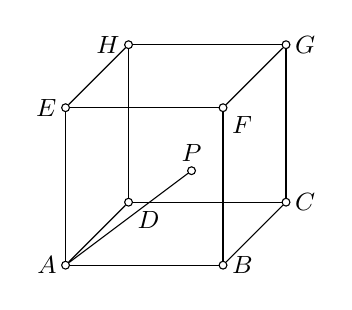
\begin{tikzpicture}
				\begin{scope}
				\small
				\tikzstyle{vnode}=[draw,circle,inner sep =1pt];
				\node[vnode] (v000) at (0,0) {};
				\node[anchor =north west] (t000) at (v000) {$D$};
				\node[vnode] (v001) at (0,2) {$$};
				\node[anchor =east] (t000) at (v001) {$H$};
				\node[vnode] (v011) at (2,2) {$$};
				\node[anchor =west] (t011) at (v011) {$G$};
				\node[vnode] (v010) at (2,0) {$$};
				\node[anchor =west] (t010) at (v010) {$C$};
				\node[vnode] (v100) at (-.8,-.8) {$$};
				\node[anchor =east] (t100) at (v100) {$A$};
				\node[vnode] (v101) at (-.8,1.2) {$$};
				\node[anchor =east] (t101) at (v101) {$E$};
				\node[vnode] (v111) at (1.2,1.2) {$$};
				\node[anchor =north west] (t111) at (v111) {$F$};
				\node[vnode] (v110) at (1.2,-0.8) {$$};
				\node[anchor =west] (t110) at (v110) {$B$};
				\node[vnode] (vP) at (.8,.4) {$$};
				\node[anchor =south] (tP) at (vP) {$P$};
				\draw (v100) to[dashed] (vP);
				\foreach \i in {01,10,11}{
						\draw (v0\i) to (v1\i);
						\draw (v\i  0) to (v\i 1);
				}
				\draw (v000) to[dashed] (v100);
				\draw (v000) to[dashed] (v010);
				\draw (v000) to[dashed] (v001);
				\draw (v001) to (v011);
				\draw (v100) to (v110);
				\draw (v101) to (v111);
				\end{scope}
			\end{tikzpicture}
        \end{QBODY}
        \begin{QFROMS}
        \end{QFROMS}
        \begin{QTAGS}\QTAG{B4C1-1空間概念}\QTAG{B4C1空間向量}\end{QTAGS}
        \begin{QANS}
            $\dfrac{5}{6}$
        \end{QANS}
        \begin{QSOLLIST}
        \end{QSOLLIST}
        \begin{QEMPTYSPACE}
        \end{QEMPTYSPACE}
    \end{QUESTION}
\end{QUESTIONS}

% !TEX encoding = UTF-8 Unicode
% !TEX TS-program = xelatex 
\begin{QUESTIONS}
    \begin{QUESTION}
        \begin{ExamInfo}{095}{學測}{單選}{1}
        \end{ExamInfo}
        \begin{ExamAnsRateInfo}{73}{97}{75}{47}
        \end{ExamAnsRateInfo}
        \begin{QBODY}
			設一元二次整係數方程式 $ax^2 + bx + c = 0$ 有一根為 $4 + 3i$。 若將此方程式的兩根與原點在複數平面上標出,則此三點所圍成的三角形面積為 
			\begin{QOPS} 
				\QOP 5 
				\QOP 6 
				\QOP 12 
				\QOP 16
				\QOP 24
			\end{QOPS}
        \end{QBODY}
        \begin{QFROMS}
        \end{QFROMS}
        \begin{QTAGS}\QTAG{B3C1三角}\end{QTAGS}
        \begin{QANS}
            (5)
        \end{QANS}
        \begin{QSOLLIST}
        \end{QSOLLIST}
        \begin{QEMPTYSPACE}
        \end{QEMPTYSPACE}
    \end{QUESTION}
    \begin{QUESTION}
        \begin{ExamInfo}{095}{學測}{單選}{2}
        \end{ExamInfo}
        \begin{ExamAnsRateInfo}{40}{73}{38}{9}
        \end{ExamAnsRateInfo}
        \begin{QBODY}
			在右圖的棋盤方格中,隨機任意取兩個格子。選出的兩個格子不在同行(有無同列無所謂)的機率為
			\begin{QOPS} 
				\QOP $\frac{1}{20}$ 
				\QOP $\frac{1}{4}$ 
				\QOP $\frac{3}{4}$
				\QOP $\frac{3}{5}$ 
				\QOP $\frac{4}{5}$
			\end{QOPS}
			
\begin{tikzpicture}[scale=.5]
				\foreach \y in {0,1,2,3,4}{
						\draw (0,\y) to (4,\y);
						\draw (\y,0) to (\y,4);
				}
			\end{tikzpicture}
        \end{QBODY}
        \begin{QFROMS}
        \end{QFROMS}
        \begin{QTAGS}\QTAG{B2C3機率}\end{QTAGS}
        \begin{QANS}
            (4)
        \end{QANS}
        \begin{QSOLLIST}
        \end{QSOLLIST}
        \begin{QEMPTYSPACE}
        \end{QEMPTYSPACE}
    \end{QUESTION}
    \begin{QUESTION}
        \begin{ExamInfo}{095}{學測}{單選}{3}
        \end{ExamInfo}
        \begin{ExamAnsRateInfo}{52}{88}{46}{22}
        \end{ExamAnsRateInfo}
        \begin{QBODY}
			右圖是由三個直角三角形堆疊而成的圖形,且 $\overline{OD} = 8$ 。
			問:直角三角形 $OAB$ 的高 $\overline{AB}$ 為何?
			\begin{QOPS} 
				\QOP $1$
				\QOP $\sqrt{6}-\sqrt{2}$ 
				\QOP $\sqrt{7}-1$ 
				\QOP $\sqrt{3}$ 
				\QOP $2$
			\end{QOPS}
			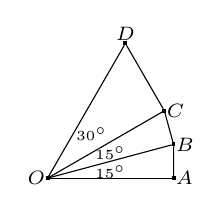
\begin{tikzpicture}[inner sep=0pt,scale=.8]\scriptsize
				\node (O) at (0,0) [label=180:$O$,draw,fill]{}; 
				\node (A) at (2,0) [label=0:$A$,draw,fill]{}; 
				\node (B) at (15:2.07) [label=0:$B$,draw,fill]{}; 
				\node (C) at (30:2.14) [label=0:$C$,draw,fill]{}; 
				\node (D) at (60:2.47) [label=90:$D$,draw,fill]{}; 
				\draw (0,0) to (A);
				\draw (0,0) to (B);
				\draw (0,0) to (C);
				\draw (0,0) to (D);
				\draw (A) to (B);
				\draw (B) to (C);
				\draw (C) to (D);
				\tiny
				\node at (.7,.7) {$30^\circ$};
				\node at (1,.4) {$15^\circ$};
				\node at (1,.1) {$15^\circ$};
			\end{tikzpicture}
        \end{QBODY}
        \begin{QFROMS}
        \end{QFROMS}
        \begin{QTAGS}\QTAG{B3C1三角}\end{QTAGS}
        \begin{QANS}
            (4)
        \end{QANS}
        \begin{QSOLLIST}
        \end{QSOLLIST}
        \begin{QEMPTYSPACE}
        \end{QEMPTYSPACE}
    \end{QUESTION}
    \begin{QUESTION}
        \begin{ExamInfo}{095}{學測}{單選}{4}
        \end{ExamInfo}
        \begin{ExamAnsRateInfo}{34}{67}{23}{12}
        \end{ExamAnsRateInfo}
        \begin{QBODY}
			下列哪一個數值最接近 $-\sqrt{2}$ ? 
			\begin{QOPS} 
				\QOP $\sqrt{3}\cos{44^\circ}+ \sin{44^\circ}$ 
				\QOP $\sqrt{3}\cos{54^\circ}+ \sin{54^\circ}$ 
				\QOP $\sqrt{3}\cos{64^\circ} +\sin{64^\circ}$
				\QOP $\sqrt{3}\cos{74^\circ}+\sin{74^\circ}$
				\QOP $\sqrt{3}\cos{84^\circ}+i\sin{84^\circ}$
			\end{QOPS}
        \end{QBODY}
        \begin{QFROMS}
        \end{QFROMS}
        \begin{QTAGS}\QTAG{B3C1三角}\end{QTAGS}
        \begin{QANS}
            (4)
        \end{QANS}
        \begin{QSOLLIST}
        \end{QSOLLIST}
        \begin{QEMPTYSPACE}
        \end{QEMPTYSPACE}
    \end{QUESTION}
    \begin{QUESTION}
        \begin{ExamInfo}{095}{學測}{單選}{5}
        \end{ExamInfo}
        \begin{ExamAnsRateInfo}{24}{50}{15}{7}
        \end{ExamAnsRateInfo}
        \begin{QBODY}
			在養分充足的情況下,細菌的數量會以指數函數的方式成長,假設細菌 $A$ 的數量每兩個小時可以成長為兩倍,細菌 $B$ 的數量每三個小時可以成長為三倍。若養分充足且一開始兩種細菌的數量相等,則大約幾小時後細菌 $B$ 的數量除以細菌 $A$ 的數量最接近 10 ? 
			\begin{QOPS} 
				\QOP $24 $小時    
				\QOP $48 $小時    
				\QOP $69 $小時 
				\QOP $96 $小時    
				\QOP $117$ 小時
			\end{QOPS}
        \end{QBODY}
        \begin{QFROMS}
        \end{QFROMS}
        \begin{QTAGS}\QTAG{B1C3指對數函數}\end{QTAGS}
        \begin{QANS}
            (5)
        \end{QANS}
        \begin{QSOLLIST}
        \end{QSOLLIST}
        \begin{QEMPTYSPACE}
        \end{QEMPTYSPACE}
    \end{QUESTION}
\end{QUESTIONS}
\begin{QUESTIONS}
    \begin{QUESTION}
        \begin{ExamInfo}{095}{學測}{多選}{6}
        \end{ExamInfo}
        \begin{ExamAnsRateInfo}{15}{27}{8}{10}
        \end{ExamAnsRateInfo}
        \begin{QBODY}
			假設 $a, b, c$ 是三個正整數。若 25 是 $a$, $b$ 的最大公因數,且 $3,4,14$ 都是 $b,c$ 的公因數,則下列何者正確?
				\begin{QOPS} 
					\QOP $c$ 一定可以被 56 整除。 
					\QOP 若 $a \leq 100$,則 $a=25$。 
					\QOP $a, b, c$ 三個數的最大公因數是 25	的因數。
					\QOP $a,b,c$ 三個數的最小公倍數大於或等於 $25 \times 3 \times 4 \times 14$ 。
				\end{QOPS}
        \end{QBODY}
        \begin{QFROMS}
        \end{QFROMS}
        \begin{QTAGS}\QTAG{綜合}\end{QTAGS}
        \begin{QANS}
            (2)(3)(4)
        \end{QANS}
        \begin{QSOLLIST}
        \end{QSOLLIST}
        \begin{QEMPTYSPACE}
        \end{QEMPTYSPACE}
    \end{QUESTION}
    \begin{QUESTION}
        \begin{ExamInfo}{095}{學測}{多選}{7}
        \end{ExamInfo}
        \begin{ExamAnsRateInfo}{47}{83}{44}{14}
        \end{ExamAnsRateInfo}
        \begin{QBODY}
			考慮坐標平面上所有滿足 $\sqrt{(x-2)^2 +y^2} + \sqrt{(x-2)^2 +(y+4)^2} =10$ 的點 $(x,y)$ 所成的圖形,下列敘述何者正確? 
			\begin{QOPS} 
				\QOP 此圖形為一橢圓。
				\QOP 此圖形為一雙曲線。 
				\QOP 此圖形的中心在 $(2,-2)$。
				\QOP 此圖形對稱於 $x-2=0$。    
				\QOP 此圖形有一頂點 $(2, 3)$ 。
			\end{QOPS}
        \end{QBODY}
        \begin{QFROMS}
        \end{QFROMS}
        \begin{QTAGS}\QTAG{B4C4二次曲線}\end{QTAGS}
        \begin{QANS}
            (1)(3)(4)(5)
        \end{QANS}
        \begin{QSOLLIST}
        \end{QSOLLIST}
        \begin{QEMPTYSPACE}
        \end{QEMPTYSPACE}
    \end{QUESTION}
    \begin{QUESTION}
        \begin{ExamInfo}{095}{學測}{多選}{8}
        \end{ExamInfo}
        \begin{ExamAnsRateInfo}{38}{71}{33}{10}
        \end{ExamAnsRateInfo}
        \begin{QBODY}
			假設實數 $a_1$, $a_2$, $a_3$, $a_4$ 是一個等差數列,且滿足 $0<a_1 <2$ 及 $a_3 =4$。若定義 $b_n =2^{a_n}$ , 則以下哪些選項是對的?
		\begin{QOPS} 
			\QOP $b_1 ,b_2 ,b_3 ,b_4$ 是一個等比數列 
			\QOP $b_1 <b_{2}$     
			\QOP $b_2 >4$ 
			\QOP $b_4 > 32$
			\QOP $b_2 \times b_4 =256$
		\end{QOPS}
        \end{QBODY}
        \begin{QFROMS}
        \end{QFROMS}
        \begin{QTAGS}\QTAG{B1C3指對數函數}\end{QTAGS}
        \begin{QANS}
            (1)(2)(3)(4)(5)
        \end{QANS}
        \begin{QSOLLIST}
        \end{QSOLLIST}
        \begin{QEMPTYSPACE}
        \end{QEMPTYSPACE}
    \end{QUESTION}
    \begin{QUESTION}
        \begin{ExamInfo}{095}{學測}{多選}{9}
        \end{ExamInfo}
        \begin{ExamAnsRateInfo}{38}{71}{30}{13}
        \end{ExamAnsRateInfo}
        \begin{QBODY}
			學生練習計算三次多項式 $f (x)$ 除以一次多項式 $g(x)$ 的餘式。
			已知 $f (x)$ 的三次項係數為 3, 一次項係數為 2。
			甲生在計算時把 $f(x)$ 的三次項係數錯看成 2 (其它係數沒看錯),
			乙生在計算時把 $f (x)$ 的一次項係數錯看成 $-2$ (其它係數沒看錯)。
			而甲生和乙生算出來的餘式剛好一樣。試問 $g(x)$ 可能等於以下哪些一次式?

			\begin{QOPSINONELINE} 
				\QOP $x$    \QOP $x-1$    \QOP $x-2$    \QOP $x+1$    \QOP $x+2$
			\end{QOPSINONELINE}
        \end{QBODY}
        \begin{QFROMS}
        \end{QFROMS}
        \begin{QTAGS}\QTAG{B1C2多項式函數}\end{QTAGS}
        \begin{QANS}
            (1)(3)(5)
        \end{QANS}
        \begin{QSOLLIST}
        \end{QSOLLIST}
        \begin{QEMPTYSPACE}
        \end{QEMPTYSPACE}
    \end{QUESTION}
    \begin{QUESTION}
        \begin{ExamInfo}{095}{學測}{多選}{10}
        \end{ExamInfo}
        \begin{ExamAnsRateInfo}{27}{48}{23}{10}
        \end{ExamAnsRateInfo}
        \begin{QBODY}
			下圖是根據 100 名婦女的體重所 作出的直方圖(圖中百分比數字代表各體重區間的相對次數,其中各區間不包含左端點而包含右端點)。該 100 名婦女體重的平均數 為 55 公斤,標準差為 12.5 公 斤。曲線 $N$ 代表一常態分佈,其平均數與標準差與樣本值相同。在此樣本中,若定義「體重過重」的標準為體重超過樣本平均數 2 個標準差以上(即體重超過 80 公斤以上),則下列敘述哪些正確? 
			\begin{QOPS} 
				\QOP 曲線 $N$ (常態分佈)中,在 55 公斤以上所佔的比例約為 $50\%$。 
				\QOP 曲線 $N$ (常態分佈)中,在 80 公斤以上所佔的比例約為 $2.5\%$ 。  
				\QOP 該樣本中,體重的中位數大於 55 公斤。 
				\QOP 該樣本中,體重的第一四分位數大於 45 公斤。 
				\QOP 該樣本中,「體重過重」(體重超過 80 公斤以上)的比例大於或等於 $5\%$。
			\end{QOPS}
			
			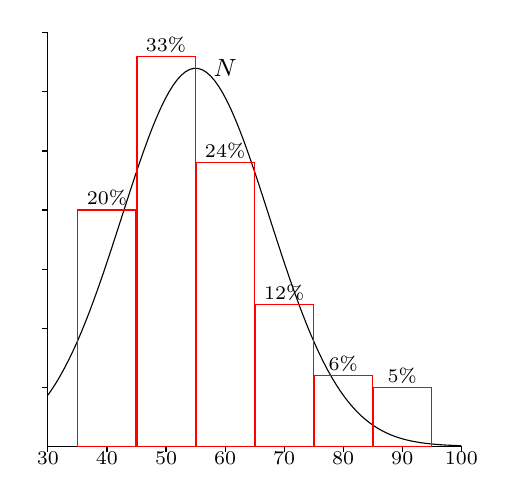
\begin{tikzpicture}[xscale=.75,yscale=.15]
				\node at (6,32) {\small $N$};
				\draw[domain=3:10,samples=100] plot (\x,{32*exp(-(\x-5.5)*(\x-5.5)/3.125)}) {};
				\begin{scope}[ybar]
				\draw (3,0) to (10,0);
				\draw (3,0) to(3,35);
				\foreach \i in {5,10,...,35}{
						\draw (3,\i) to (2.9,\i);
				}
				\foreach \i in {30,40,50,...,100}{
						\node at (0.1*\i,-1) {\scriptsize \i};
						\draw (0.1*\i,0) to (0.1*\i,-.5);
				}
				\foreach \i/\j in {40/20,50/33,60/24,70/12,80/6,90/5}{
						\node at (0.1*\i,\j+1) {\scriptsize \j $\%$};
				}
				\draw[color=red,bar width=28pt]
					plot coordinates{(4,20) (5,33) (6,24) (7,12) (8,6) (9,5) };
				\end{scope}
			\end{tikzpicture}
        \end{QBODY}
        \begin{QFROMS}
        \end{QFROMS}
        \begin{QTAGS}\QTAG{B5C1機率與統計}\end{QTAGS}
        \begin{QANS}
            (1)(2)(4)(5)
        \end{QANS}
        \begin{QSOLLIST}
        \end{QSOLLIST}
        \begin{QEMPTYSPACE}
        \end{QEMPTYSPACE}
    \end{QUESTION}
    \begin{QUESTION}
        \begin{ExamInfo}{095}{學測}{多選}{11}
        \end{ExamInfo}
        \begin{ExamAnsRateInfo}{76}{98}{89}{41}
        \end{ExamAnsRateInfo}
        \begin{QBODY}
			將正整數 18 分解成兩個正整數的乘積有 $1\times 18$ , $2\times 9$, $3\times 6$ 三種,又 $3 \times 6$ 是這三種分解中,兩數的差最小的,我們稱 $3 \times 6$ 為 18 的最佳分解。當 $p\times q (p \leq q)$ 是正整數 $n$ 的最佳分解時,我們規定函數 $F(n)=\frac{p}{q}$,例如 $F(18)=\frac{3}{6}=\frac{1}{2}$。
			下列有關函數 $F(n)$ 的敘述,何者正確? 
			\begin{QOPS} 
				\QOP $F(4) =1$    \QOP $F(24)=\frac{3}{8}$ 
				\QOP $F(27)=\frac{1}{3}$ 
				\QOP 若 $n$ 是一個質數,則 $F(n)=\frac{1}{n}$ 
				\QOP 若 $n$ 是一個完全平方數,則 $F(n) =1$。
			\end{QOPS}
        \end{QBODY}
        \begin{QFROMS}
        \end{QFROMS}
        \begin{QTAGS}\QTAG{綜合}\end{QTAGS}
        \begin{QANS}
            (1)(3)(4)(5)
        \end{QANS}
        \begin{QSOLLIST}
        \end{QSOLLIST}
        \begin{QEMPTYSPACE}
        \end{QEMPTYSPACE}
    \end{QUESTION}
\end{QUESTIONS}
\begin{QUESTIONS}
    \begin{QUESTION}
        \begin{ExamInfo}{095}{學測}{填充}{A}
        \end{ExamInfo}
        \begin{ExamAnsRateInfo}{44}{80}{44}{8}
        \end{ExamAnsRateInfo}
        \begin{QBODY}
			抽樣調查某地區 1000 個有兩個小孩的家庭,得到如下數據,其中 (男,女) 代表第一個小孩是男孩而第二個小孩是女生的家庭,餘類推。由此數據可估計該地區有兩個小孩家庭的男、女孩性別比約為 $\TCNBOX{\TCN\TCN\TCN}:100 $(四捨五入至整數位)。
        \end{QBODY}
        \begin{QFROMS}
        \end{QFROMS}
        \begin{QTAGS}\QTAG{綜合}\end{QTAGS}
        \begin{QANS}
            $105$
        \end{QANS}
        \begin{QSOLLIST}
        \end{QSOLLIST}
        \begin{QEMPTYSPACE}
        \end{QEMPTYSPACE}
    \end{QUESTION}
    \begin{QUESTION}
        \begin{ExamInfo}{095}{學測}{填充}{B}
        \end{ExamInfo}
        \begin{ExamAnsRateInfo}{33}{77}{21}{1}
        \end{ExamAnsRateInfo}
        \begin{QBODY}
			右圖為一正立方體, 若 $M$ 在線段 $\overline{AB}$ 上,$\overline{BM} = 2\overline{AM}$, $N$ 為線段 $\overline{BC}$ 之中點,則 $\cos \angle MON = \TCNBOX{\FR{\TCN\sqrt{\TCN\TCN}}{\TCN\TCN}}$ 。(分數要化成最簡分數)
		
			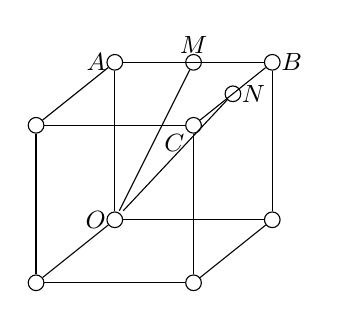
\begin{tikzpicture}
				\begin{scope}
				\small
				\node (vO) at (0,0) {};
				\tikzstyle{vnode}=[draw,circle,inner sep =2pt];
				\node[vnode] (v000) at (0,0) {};
				\node[anchor =east] (t000) at (v000) {$O$};
				%\fill [red] ($(a) + 1/3*(1cm,0)$) circle (2pt);
				\node[vnode] (v001) at (0,2) {$$};
				\node[anchor =east] (t000) at (v001) {$A$};
				\node[vnode] (v011) at (2,2) {$$};
				\node[anchor =west] (t011) at (v011) {$B$};
				\node[vnode] (v010) at (2,0) {$$};
				\node[anchor =west] (t010) at (v010) {$$};
				\node[vnode] (v100) at (-1.0,-.8) {$$};
				\node[anchor =west] (t100) at (v100) {$$};
				\node[vnode] (v101) at (-1.0,1.2) {$$};
				\node[anchor =west] (t101) at (v101) {$$};
				\node[vnode] (v111) at (1.0,1.2) {$$};
				\node[anchor =north east] (t111) at (v111) {$C$};
				\node[vnode] (v110) at (1.0,-0.8) {$$};
				\node[anchor =west] (t110) at (v110) {$$};
				\node[vnode] (vM) at (1,2) {$$};
				\node[anchor =south] (tM) at (vM) {$M$};
				\node[vnode] (vN) at (1.5,1.6) {$$};
				\node[anchor =west] (tN) at (vN) {$N$};
				\draw (vM) to[dashed] (vO);
				\draw (vN) to[dashed] (vO);
				\foreach \i in {01,10,11}{
						\draw (v0\i) to (v1\i);
						\draw (v\i  0) to (v\i 1);
				}
				\draw (v000) to[dashed] (v100);
				\draw (v000) to[dashed] (v010);
				\draw (v000) to[dashed] (v001);
				\draw (v001) to (v011);
				\draw (v100) to (v110);
				\draw (v101) to (v111);
				\end{scope}
			\end{tikzpicture}
        \end{QBODY}
        \begin{QFROMS}
        \end{QFROMS}
        \begin{QTAGS}\QTAG{B4C1空間向量}\end{QTAGS}
        \begin{QANS}
            $\frac{4\sqrt{10}}{15}$
        \end{QANS}
        \begin{QSOLLIST}
        \end{QSOLLIST}
        \begin{QEMPTYSPACE}
        \end{QEMPTYSPACE}
    \end{QUESTION}
    \begin{QUESTION}
        \begin{ExamInfo}{095}{學測}{填充}{C}
        \end{ExamInfo}
        \begin{ExamAnsRateInfo}{49}{88}{50}{9}
        \end{ExamAnsRateInfo}
        \begin{QBODY}
			給定平面上三點 $(-6, -2)$, $(2, -1)$, $(1, 2)$。若有第四點和此三點形成一菱形(四邊長皆相等),則第四點的坐標為 $\TCNBOX{(\TCN,\TCN)}$ 。
        \end{QBODY}
        \begin{QFROMS}
        \end{QFROMS}
        \begin{QTAGS}\QTAG{B3C3平面向量}\end{QTAGS}
        \begin{QANS}
            $(9,3)$
        \end{QANS}
        \begin{QSOLLIST}
        \end{QSOLLIST}
        \begin{QEMPTYSPACE}
        \end{QEMPTYSPACE}
    \end{QUESTION}
    \begin{QUESTION}
        \begin{ExamInfo}{095}{學測}{填充}{D}
        \end{ExamInfo}
        \begin{ExamAnsRateInfo}{34}{72}{26}{4}
        \end{ExamAnsRateInfo}
        \begin{QBODY}
			$ABCD$ 為圓內接四邊形,若 $\angle DBC = 30 ^\circ$, $\angle ABD = 45^\circ$, $\overline{CD}=6$,則線段 $\overline{AD}= \TCNBOX{\sqrt{\TCN\TCN}}$ 。
        \end{QBODY}
        \begin{QFROMS}
        \end{QFROMS}
        \begin{QTAGS}\QTAG{B3C1三角}\end{QTAGS}
        \begin{QANS}
            $\sqrt{72}$
        \end{QANS}
        \begin{QSOLLIST}
        \end{QSOLLIST}
        \begin{QEMPTYSPACE}
        \end{QEMPTYSPACE}
    \end{QUESTION}
    \begin{QUESTION}
        \begin{ExamInfo}{095}{學測}{填充}{E}
        \end{ExamInfo}
        \begin{ExamAnsRateInfo}{68}{89}{75}{40}
        \end{ExamAnsRateInfo}
        \begin{QBODY}
			新新鞋店為與同業進行促銷戰,推出「第二雙不用錢:買一送一」的活動。該鞋店共有八款 鞋可供選擇,其價格如下:規定所送的鞋之價格一定少於所買的價格(例如:買一個「丁」款鞋,可送甲、乙兩款鞋 之一)。若有一位新新鞋店的顧客買一送一,則該顧客所帶走的兩雙鞋,其搭配方法一共有款式 
			$\TCNBOX{\TCN\TCN}$ 種。 
			\vspace*{0cm} 
			\begin{center}\begin{tabular}{|c|c|c|c|c|c|c|c|c|}  \hline 
			款式 & 甲 &乙 &丙 & 丁 &戊 & 己& 庚& 辛 \\ \hline 
			價格 & 670 & 670 & 700  & 700  & 700  & 800   & 800  & 800\\\hline
			\end{tabular}\end{center}
        \end{QBODY}
        \begin{QFROMS}
        \end{QFROMS}
        \begin{QTAGS}\QTAG{B2C2排列組合}\end{QTAGS}
        \begin{QANS}
            $21$
        \end{QANS}
        \begin{QSOLLIST}
        \end{QSOLLIST}
        \begin{QEMPTYSPACE}
        \end{QEMPTYSPACE}
    \end{QUESTION}
    \begin{QUESTION}
        \begin{ExamInfo}{095}{學測}{填充}{F}
        \end{ExamInfo}
        \begin{ExamAnsRateInfo}{44}{81}{44}{7}
        \end{ExamAnsRateInfo}
        \begin{QBODY}
		某地共有 9 個電視頻道,將其分配給 3 個新聞台、4 個綜藝台及 2 個體育台共三種類型。 若同類型電視台的頻道要相鄰,而且前兩個頻道保留給體育台,則頻道的分配方式共有 $\TCNBOX{\TCN\TCN\TCN}$ 種。
        \end{QBODY}
        \begin{QFROMS}
        \end{QFROMS}
        \begin{QTAGS}\QTAG{B2C2排列組合}\end{QTAGS}
        \begin{QANS}
            $576$
        \end{QANS}
        \begin{QSOLLIST}
        \end{QSOLLIST}
        \begin{QEMPTYSPACE}
        \end{QEMPTYSPACE}
    \end{QUESTION}
    \begin{QUESTION}
        \begin{ExamInfo}{095}{學測}{填充}{G}
        \end{ExamInfo}
        \begin{ExamAnsRateInfo}{71}{93}{79}{41}
        \end{ExamAnsRateInfo}
        \begin{QBODY}
			用黑、白兩種顏色的正方形地磚依照如下的規律拼成若干圖形:\bigskip

		\begin{tikzpicture}[scale=.5] \small
		\foreach \x in {0,1,2,3,6,7,8,9,10,11,14,15,16,17,18,19,20,21}
						\draw (\x,0) to (\x,3);
		\foreach \a/\b in {1/2, 7/8,9/10,15/16,17/18,19/20}
		\draw[fill] (\a,1) rectangle (\b,2);
		\foreach \x/\t in {1.5/第一個, 8.5/第二個, 17.5/第三個}
				\node at (\x,-1) {\t};
		\foreach \y in {0,1,2,3}{
				\draw (0,\y) to (3,\y);
				\draw (6,\y) to (11,\y);
				\draw (14,\y) to (21,\y);
		}
		\end{tikzpicture}
		\bigskip
		
		拼第 95 個圖需用到 $\TCNBOX{\TCN\TCN}$ 塊白色地磚。
        \end{QBODY}
        \begin{QFROMS}
        \end{QFROMS}
        \begin{QTAGS}\QTAG{B2C1數列級數}\end{QTAGS}
        \begin{QANS}
            $478$
        \end{QANS}
        \begin{QSOLLIST}
        \end{QSOLLIST}
        \begin{QEMPTYSPACE}
        \end{QEMPTYSPACE}
    \end{QUESTION}
    \begin{QUESTION}
        \begin{ExamInfo}{095}{學測}{填充}{H}
        \end{ExamInfo}
        \begin{ExamAnsRateInfo}{51}{84}{47}{22}
        \end{ExamAnsRateInfo}
        \begin{QBODY}
			在三角形 $ABC$ 中,若 $D$ 點在 $\overline{BC}$ 邊上,且 $\overline{AB}=7$, $\overline{AC}=13$, $\overline{BD}=7$, $\overline{CD}=8$,則 $\overline{AD}=\TCNBOX{\TCN}$。
        \end{QBODY}
        \begin{QFROMS}
        \end{QFROMS}
        \begin{QTAGS}\QTAG{B3C1三角}\end{QTAGS}
        \begin{QANS}
            $7$
        \end{QANS}
        \begin{QSOLLIST}
        \end{QSOLLIST}
        \begin{QEMPTYSPACE}
        \end{QEMPTYSPACE}
    \end{QUESTION}
    \begin{QUESTION}
        \begin{ExamInfo}{095}{學測}{填充}{I}
        \end{ExamInfo}
        \begin{ExamAnsRateInfo}{25}{56}{12}{7}
        \end{ExamAnsRateInfo}
        \begin{QBODY}
			設 $A(0,0)$, $B(10,0)$, $C(10,6)$, $D(0,6)$ 為坐標平面上的四個點。如果直線 $y=m(x-7)+4$ 將四邊形 $ABCD$ 分成面積相等的兩塊,那麼 $m= \TCNBOX{\FR{\TCN}{\TCN}}$。
        \end{QBODY}
        \begin{QFROMS}
        \end{QFROMS}
        \begin{QTAGS}\QTAG{B3C2直線與圓}\end{QTAGS}
        \begin{QANS}
            $ \frac{1}{2}$
        \end{QANS}
        \begin{QSOLLIST}
        \end{QSOLLIST}
        \begin{QEMPTYSPACE}
        \end{QEMPTYSPACE}
    \end{QUESTION}
\end{QUESTIONS}

% !TEX encoding = UTF-8 Unicode
% !TEX TS-program = xelatex 
\begin{QUESTIONS}
    \begin{QUESTION}
        \begin{ExamInfo}{096}{學測}{單選}{1}
        \end{ExamInfo}
        \begin{ExamAnsRateInfo}{71}{95}{81}{37}
        \end{ExamAnsRateInfo}
        \begin{QBODY}
        \end{QBODY}
        \begin{QFROMS}
        \end{QFROMS}
        \begin{QTAGS}\QTAG{B1C2多項式函數}\end{QTAGS}
        \begin{QANS}
            (4)
        \end{QANS}
        \begin{QSOLLIST}
        \end{QSOLLIST}
        \begin{QEMPTYSPACE}
        \end{QEMPTYSPACE}
    \end{QUESTION}
    \begin{QUESTION}
        \begin{ExamInfo}{096}{學測}{單選}{2}
        \end{ExamInfo}
        \begin{ExamAnsRateInfo}{35}{58}{28}{19}
        \end{ExamAnsRateInfo}
        \begin{QBODY}
        \end{QBODY}
        \begin{QFROMS}
        \end{QFROMS}
        \begin{QTAGS}\QTAG{綜合}\end{QTAGS}
        \begin{QANS}
            (2)
        \end{QANS}
        \begin{QSOLLIST}
        \end{QSOLLIST}
        \begin{QEMPTYSPACE}
        \end{QEMPTYSPACE}
    \end{QUESTION}
    \begin{QUESTION}
        \begin{ExamInfo}{096}{學測}{單選}{3}
        \end{ExamInfo}
        \begin{ExamAnsRateInfo}{58}{88}{62}{24}
        \end{ExamAnsRateInfo}
        \begin{QBODY}
        \end{QBODY}
        \begin{QFROMS}
        \end{QFROMS}
        \begin{QTAGS}\QTAG{B1C2多項式函數}\end{QTAGS}
        \begin{QANS}
            (4)
        \end{QANS}
        \begin{QSOLLIST}
        \end{QSOLLIST}
        \begin{QEMPTYSPACE}
        \end{QEMPTYSPACE}
    \end{QUESTION}
    \begin{QUESTION}
        \begin{ExamInfo}{096}{學測}{單選}{4}
        \end{ExamInfo}
        \begin{ExamAnsRateInfo}{47}{78}{46}{17}
        \end{ExamAnsRateInfo}
        \begin{QBODY}
        \end{QBODY}
        \begin{QFROMS}
        \end{QFROMS}
        \begin{QTAGS}\QTAG{B4C4二次曲線}\end{QTAGS}
        \begin{QANS}
            (1)
        \end{QANS}
        \begin{QSOLLIST}
        \end{QSOLLIST}
        \begin{QEMPTYSPACE}
        \end{QEMPTYSPACE}
    \end{QUESTION}
    \begin{QUESTION}
        \begin{ExamInfo}{096}{學測}{單選}{5}
        \end{ExamInfo}
        \begin{ExamAnsRateInfo}{47}{67}{46}{28}
        \end{ExamAnsRateInfo}
        \begin{QBODY}
        \end{QBODY}
        \begin{QFROMS}
        \end{QFROMS}
        \begin{QTAGS}\QTAG{B3C1三角}\end{QTAGS}
        \begin{QANS}
            (3)
        \end{QANS}
        \begin{QSOLLIST}
        \end{QSOLLIST}
        \begin{QEMPTYSPACE}
        \end{QEMPTYSPACE}
    \end{QUESTION}
\end{QUESTIONS}
\begin{QUESTIONS}
    \begin{QUESTION}
        \begin{ExamInfo}{096}{學測}{多選}{6}
        \end{ExamInfo}
        \begin{ExamAnsRateInfo}{19}{35}{12}{10}
        \end{ExamAnsRateInfo}
        \begin{QBODY}
        \end{QBODY}
        \begin{QFROMS}
        \end{QFROMS}
        \begin{QTAGS}\QTAG{B3C1三角}\end{QTAGS}
        \begin{QANS}
            (1)(3)(5)
        \end{QANS}
        \begin{QSOLLIST}
        \end{QSOLLIST}
        \begin{QEMPTYSPACE}
        \end{QEMPTYSPACE}
    \end{QUESTION}
    \begin{QUESTION}
        \begin{ExamInfo}{096}{學測}{多選}{7}
        \end{ExamInfo}
        \begin{ExamAnsRateInfo}{25}{42}{20}{13}
        \end{ExamAnsRateInfo}
        \begin{QBODY}
        \end{QBODY}
        \begin{QFROMS}
        \end{QFROMS}
        \begin{QTAGS}\QTAG{B3C3平面向量}\end{QTAGS}
        \begin{QANS}
            (1)(2)(4)(5)
        \end{QANS}
        \begin{QSOLLIST}
        \end{QSOLLIST}
        \begin{QEMPTYSPACE}
        \end{QEMPTYSPACE}
    \end{QUESTION}
    \begin{QUESTION}
        \begin{ExamInfo}{096}{學測}{多選}{8}
        \end{ExamInfo}
        \begin{ExamAnsRateInfo}{30}{36}{32}{22}
        \end{ExamAnsRateInfo}
        \begin{QBODY}
        \end{QBODY}
        \begin{QFROMS}
        \end{QFROMS}
        \begin{QTAGS}\QTAG{B4C3矩陣}\end{QTAGS}
        \begin{QANS}
            (1)(5)
        \end{QANS}
        \begin{QSOLLIST}
        \end{QSOLLIST}
        \begin{QEMPTYSPACE}
        \end{QEMPTYSPACE}
    \end{QUESTION}
    \begin{QUESTION}
        \begin{ExamInfo}{096}{學測}{多選}{9}
        \end{ExamInfo}
        \begin{ExamAnsRateInfo}{42}{70}{39}{17}
        \end{ExamAnsRateInfo}
        \begin{QBODY}
        \end{QBODY}
        \begin{QFROMS}
        \end{QFROMS}
        \begin{QTAGS}\QTAG{B4C1空間向量}\end{QTAGS}
        \begin{QANS}
            (1)(2)(4)
        \end{QANS}
        \begin{QSOLLIST}
        \end{QSOLLIST}
        \begin{QEMPTYSPACE}
        \end{QEMPTYSPACE}
    \end{QUESTION}
    \begin{QUESTION}
        \begin{ExamInfo}{096}{學測}{多選}{10}
        \end{ExamInfo}
        \begin{ExamAnsRateInfo}{28}{52}{21}{11}
        \end{ExamAnsRateInfo}
        \begin{QBODY}
        \end{QBODY}
        \begin{QFROMS}
        \end{QFROMS}
        \begin{QTAGS}\QTAG{B1C3指對數函數}\end{QTAGS}
        \begin{QANS}
            (1)(2)(4)(5)
        \end{QANS}
        \begin{QSOLLIST}
        \end{QSOLLIST}
        \begin{QEMPTYSPACE}
        \end{QEMPTYSPACE}
    \end{QUESTION}
    \begin{QUESTION}
        \begin{ExamInfo}{096}{學測}{多選}{11}
        \end{ExamInfo}
        \begin{ExamAnsRateInfo}{22}{35}{16}{15}
        \end{ExamAnsRateInfo}
        \begin{QBODY}
        \end{QBODY}
        \begin{QFROMS}
        \end{QFROMS}
        \begin{QTAGS}\QTAG{B1C2多項式函數}\end{QTAGS}
        \begin{QANS}
            (2)(4)
        \end{QANS}
        \begin{QSOLLIST}
        \end{QSOLLIST}
        \begin{QEMPTYSPACE}
        \end{QEMPTYSPACE}
    \end{QUESTION}
\end{QUESTIONS}
\begin{QUESTIONS}
    \begin{QUESTION}
        \begin{ExamInfo}{096}{學測}{填充}{A}
        \end{ExamInfo}
        \begin{ExamAnsRateInfo}{41}{77}{36}{10}
        \end{ExamAnsRateInfo}
        \begin{QBODY}
        \end{QBODY}
        \begin{QFROMS}
        \end{QFROMS}
        \begin{QTAGS}\QTAG{B1C3指對數函數}\end{QTAGS}
        \begin{QANS}
            $\dfrac{1}{4}$
        \end{QANS}
        \begin{QSOLLIST}
        \end{QSOLLIST}
        \begin{QEMPTYSPACE}
        \end{QEMPTYSPACE}
    \end{QUESTION}
    \begin{QUESTION}
        \begin{ExamInfo}{096}{學測}{填充}{B}
        \end{ExamInfo}
        \begin{ExamAnsRateInfo}{27}{64}{16}{1}
        \end{ExamAnsRateInfo}
        \begin{QBODY}
        \end{QBODY}
        \begin{QFROMS}
        \end{QFROMS}
        \begin{QTAGS}\QTAG{B3C3平面向量}\end{QTAGS}
        \begin{QANS}
            $(-1,12)$
        \end{QANS}
        \begin{QSOLLIST}
        \end{QSOLLIST}
        \begin{QEMPTYSPACE}
        \end{QEMPTYSPACE}
    \end{QUESTION}
    \begin{QUESTION}
        \begin{ExamInfo}{096}{學測}{填充}{C}
        \end{ExamInfo}
        \begin{ExamAnsRateInfo}{66}{93}{76}{29}
        \end{ExamAnsRateInfo}
        \begin{QBODY}
        \end{QBODY}
        \begin{QFROMS}
        \end{QFROMS}
        \begin{QTAGS}\QTAG{B2C4數據分析}\end{QTAGS}
        \begin{QANS}
            $79$
        \end{QANS}
        \begin{QSOLLIST}
        \end{QSOLLIST}
        \begin{QEMPTYSPACE}
        \end{QEMPTYSPACE}
    \end{QUESTION}
    \begin{QUESTION}
        \begin{ExamInfo}{096}{學測}{填充}{D}
        \end{ExamInfo}
        \begin{ExamAnsRateInfo}{75}{92}{82}{51}
        \end{ExamAnsRateInfo}
        \begin{QBODY}
        \end{QBODY}
        \begin{QFROMS}
        \end{QFROMS}
        \begin{QTAGS}\QTAG{B2C1數列級數}\end{QTAGS}
        \begin{QANS}
            $1600$
        \end{QANS}
        \begin{QSOLLIST}
        \end{QSOLLIST}
        \begin{QEMPTYSPACE}
        \end{QEMPTYSPACE}
    \end{QUESTION}
    \begin{QUESTION}
        \begin{ExamInfo}{096}{學測}{填充}{E}
        \end{ExamInfo}
        \begin{ExamAnsRateInfo}{29}{66}{18}{3}
        \end{ExamAnsRateInfo}
        \begin{QBODY}
        \end{QBODY}
        \begin{QFROMS}
        \end{QFROMS}
        \begin{QTAGS}\QTAG{B3C2直線與圓}\end{QTAGS}
        \begin{QANS}
            $(\frac{12}{13},\frac{-5}{13})$
        \end{QANS}
        \begin{QSOLLIST}
        \end{QSOLLIST}
        \begin{QEMPTYSPACE}
        \end{QEMPTYSPACE}
    \end{QUESTION}
    \begin{QUESTION}
        \begin{ExamInfo}{096}{學測}{填充}{F}
        \end{ExamInfo}
        \begin{ExamAnsRateInfo}{26}{38}{28}{12}
        \end{ExamAnsRateInfo}
        \begin{QBODY}
        \end{QBODY}
        \begin{QFROMS}
        \end{QFROMS}
        \begin{QTAGS}\QTAG{B2C2排列組合}\end{QTAGS}
        \begin{QANS}
            $25$
        \end{QANS}
        \begin{QSOLLIST}
        \end{QSOLLIST}
        \begin{QEMPTYSPACE}
        \end{QEMPTYSPACE}
    \end{QUESTION}
    \begin{QUESTION}
        \begin{ExamInfo}{096}{學測}{填充}{G}
        \end{ExamInfo}
        \begin{ExamAnsRateInfo}{19}{39}{13}{5}
        \end{ExamAnsRateInfo}
        \begin{QBODY}
        \end{QBODY}
        \begin{QFROMS}
        \end{QFROMS}
        \begin{QTAGS}\QTAG{B5C1機率與統計}\end{QTAGS}
        \begin{QANS}
            $\frac{87}{14}$
        \end{QANS}
        \begin{QSOLLIST}
        \end{QSOLLIST}
        \begin{QEMPTYSPACE}
        \end{QEMPTYSPACE}
    \end{QUESTION}
    \begin{QUESTION}
        \begin{ExamInfo}{096}{學測}{填充}{H}
        \end{ExamInfo}
        \begin{ExamAnsRateInfo}{32}{63}{26}{7}
        \end{ExamAnsRateInfo}
        \begin{QBODY}
        \end{QBODY}
        \begin{QFROMS}
        \end{QFROMS}
        \begin{QTAGS}\QTAG{B4C4二次曲線}\end{QTAGS}
        \begin{QANS}
            $12$
        \end{QANS}
        \begin{QSOLLIST}
        \end{QSOLLIST}
        \begin{QEMPTYSPACE}
        \end{QEMPTYSPACE}
    \end{QUESTION}
    \begin{QUESTION}
        \begin{ExamInfo}{096}{學測}{填充}{I}
        \end{ExamInfo}
        \begin{ExamAnsRateInfo}{15}{37}{6}{2}
        \end{ExamAnsRateInfo}
        \begin{QBODY}
        \end{QBODY}
        \begin{QFROMS}
        \end{QFROMS}
        \begin{QTAGS}\QTAG{B3C3平面向量}\end{QTAGS}
        \begin{QANS}
            $5 \sqrt{3}$
        \end{QANS}
        \begin{QSOLLIST}
        \end{QSOLLIST}
        \begin{QEMPTYSPACE}
        \end{QEMPTYSPACE}
    \end{QUESTION}
\end{QUESTIONS}

% !TEX encoding = UTF-8 Unicode
% !TEX TS-program = xelatex
\begin{QUESTIONS}
    \begin{QUESTION}
        \begin{ExamInfo}{97}{學測}{單選}{1}
        \end{ExamInfo}
        \begin{ExamAnsRateInfo}{60}{92}{62}{26}
        \end{ExamAnsRateInfo}
        \begin{QBODY}
            對任意實數 $x$ 而言,$27^{(x^2 + \frac{2}{3})}$ 的最小值為 
			\begin{QOPS} 
				\QOP $3$        
				\QOP $3\sqrt{3}$
				\QOP $9$ 
				\QOP $27$
				\QOP $81\sqrt{3}$
			\end{QOPS}
        \end{QBODY}
        \begin{QFROMS}
        \end{QFROMS}
        \begin{QTAGS}\QTAG{B1C3-2指數函數}\QTAG{B1C3指對數函數}\QTAG{最值}\end{QTAGS}
        \begin{QANS}
            (3)
        \end{QANS}
        \begin{QSOLLIST}
        \end{QSOLLIST}
        \begin{QEMPTYSPACE}
        \end{QEMPTYSPACE}
    \end{QUESTION}
    \begin{QUESTION}
        \begin{ExamInfo}{97}{學測}{單選}{2}
        \end{ExamInfo}
        \begin{ExamAnsRateInfo}{75}{96}{85}{44}
        \end{ExamAnsRateInfo}
        \begin{QBODY}
            在職棒比賽中 ERA 值是了解一個投手表現的重要統計數值。其計算方式如下:若此投手共主投 $n$ 局,其總責任失分為 $E$,則其 ERA 值為 $\frac{E}{n}\times 9$ 。有一位投手在之前的比賽中共主投了 90局,且這 90 局中他的 ERA 值為 3.2。在最新的一場比賽中此投手主投 6 局無責任失分,則打完這一場比賽後,此投手的 ERA 值成為 
			\begin{QOPS} 
				\QOP 2.9 
				\QOP 3.0  
				\QOP 3.1 
				\QOP 3.2  
				\QOP 3.3
			\end{QOPS}
        \end{QBODY}
        \begin{QFROMS}
        \end{QFROMS}
        \begin{QTAGS}\QTAG{不是99課綱}\end{QTAGS}
        \begin{QANS}
            (2)
        \end{QANS}
        \begin{QSOLLIST}
        \end{QSOLLIST}
        \begin{QEMPTYSPACE}
        \end{QEMPTYSPACE}
    \end{QUESTION}
    \begin{QUESTION}
        \begin{ExamInfo}{97}{學測}{單選}{3}
        \end{ExamInfo}
        \begin{ExamAnsRateInfo}{73}{97}{84}{38}
        \end{ExamAnsRateInfo}
        \begin{QBODY}
            有一個圓形跑道分內、外兩圈,半徑分別為 30、50 公尺。今甲在內圈以等速行走、乙在外圈 以等速跑步,且知甲每走一圈,乙恰跑了兩圈。若甲走了 45 公尺,則同時段乙跑了 \\
			\begin{QOPSINONELINE} 
				\QOP 90 公尺 \QOP 120 公尺 \QOP 135 公尺 \QOP 150 公尺 \QOP 180 公尺
			\end{QOPSINONELINE}
        \end{QBODY}
        \begin{QFROMS}
        \end{QFROMS}
        \begin{QTAGS}\QTAG{不是99課綱}\end{QTAGS}
        \begin{QANS}
            (4)
        \end{QANS}
        \begin{QSOLLIST}
        \end{QSOLLIST}
        \begin{QEMPTYSPACE}
        \end{QEMPTYSPACE}
    \end{QUESTION}
    \begin{QUESTION}
        \begin{ExamInfo}{97}{學測}{單選}{4}
        \end{ExamInfo}
        \begin{ExamAnsRateInfo}{39}{69}{31}{17}
        \end{ExamAnsRateInfo}
        \begin{QBODY}
            某地區的車牌號碼共六碼,其中前兩碼為 O 以外的英文大寫字母,後四碼為 0 到 9 的阿拉伯數字,但規定不能連續出現三個 4。例如: AA1234 , AB4434 為可出現的車牌號碼;而 AO1234 ,AB3444 為不可出現的車牌號碼。則所有第一碼為 A 且最後一碼為 4 的車牌號碼個數為 
			\begin{QOPS}
				\QOP $25 \times 9^3$ 
				\QOP $25\times 9^2 \times 10$        
				\QOP $25 \times 900$
				\QOP $25 \times 990$ 
				\QOP $25 \times 999$ 
			\end{QOPS}
        \end{QBODY}
        \begin{QFROMS}
        \end{QFROMS}
        \begin{QTAGS}\QTAG{B2C2-2排列}\QTAG{重複排列}\QTAG{B2C2排列組合}\end{QTAGS}
        \begin{QANS}
            (4)
        \end{QANS}
        \begin{QSOLLIST}
        \end{QSOLLIST}
        \begin{QEMPTYSPACE}
        \end{QEMPTYSPACE}
    \end{QUESTION}
    \begin{QUESTION}
        \begin{ExamInfo}{97}{學測}{單選}{5}
        \end{ExamInfo}
        \begin{ExamAnsRateInfo}{41}{74}{32}{17}
        \end{ExamAnsRateInfo}
        \begin{QBODY}
            廣場上插了一支紅旗與一支白旗,小明站在兩支旗子之間。		利用手邊的儀器,小明測出他與正東方紅旗間的距離為他與正西方白旗間距離的 6 倍;			小明往正北方走了 10 公尺之後再量一 次,發現他與紅旗的距離變成他與白旗距離的 4 倍。			試問紅白兩旗之間的距離最接近下列哪個選項?
			\begin{QOPS} 
				\QOP 60 公尺 
				\QOP 65 公尺    
				\QOP 70 公尺 
				\QOP 75 公尺 
				\QOP 80 公尺
			\end{QOPS}
        \end{QBODY}
        \begin{QFROMS}
        \end{QFROMS}
        \begin{QTAGS}\QTAG{B3C1-5三角測量}\QTAG{B3C1三角}\end{QTAGS}
        \begin{QANS}
            (1)
        \end{QANS}
        \begin{QSOLLIST}
        \end{QSOLLIST}
        \begin{QEMPTYSPACE}
        \end{QEMPTYSPACE}
    \end{QUESTION}
\end{QUESTIONS}
\begin{QUESTIONS}
    \begin{QUESTION}
        \begin{ExamInfo}{97}{學測}{多選}{6}
        \end{ExamInfo}
        \begin{ExamAnsRateInfo}{56}{92}{58}{18}
        \end{ExamAnsRateInfo}
        \begin{QBODY}
            試問:在坐標平面上,下列哪些選項中的函數圖形完全落在 $x$ 軸的上方? 
			\begin{QOPS} 
				\QOP $y=x+100$
				\QOP $y=x^2+1$ 
				\QOP $y=2+\sin x$
				\QOP $y=2x$
				\QOP $y=\log x$
			\end{QOPS}
        \end{QBODY}
        \begin{QFROMS}
        \end{QFROMS}
        \begin{QTAGS}\QTAG{跨章節試題}\end{QTAGS}
        \begin{QANS}
            (2)(3)(4)
        \end{QANS}
        \begin{QSOLLIST}
        \end{QSOLLIST}
        \begin{QEMPTYSPACE}
        \end{QEMPTYSPACE}
    \end{QUESTION}
    \begin{QUESTION}
        \begin{ExamInfo}{97}{學測}{多選}{7}
        \end{ExamInfo}
        \begin{ExamAnsRateInfo}{39}{60}{40}{17}
        \end{ExamAnsRateInfo}
        \begin{QBODY}
            某高中共有 20 個班級,每班各有 40 位學生,其中男生 25 人,女生 15 人。若從全校 800 人中以簡單隨機抽樣抽出 80 人,試問下列哪些選項是正確的? 
			\begin{QOPS} 
				\QOP 每班至少會有一人被抽中 
				\QOP 抽出來的男生人數一定比女生人數多 
				\QOP 已知小文是男生,小美是女生,則小文被抽中的機率大於小美被抽中的機率。 
				\QOP 若學生甲和學生乙在同一班,學生丙在另外一班,則甲、乙兩人同時被抽中的機率跟甲、 丙兩人同時被抽中的機率一樣 
				\QOP 學生 $A$ 和學生 $B$ 是兄弟,他們同時被抽中的機率小於 $\frac{1}{100}$
            \end{QOPS}
        \end{QBODY}
        \begin{QFROMS}
        \end{QFROMS}
        \begin{QTAGS}\QTAG{B2C3機率}\QTAG{B2C3-2機率的定義與性質}\end{QTAGS}
        \begin{QANS}
            (4)(5)
        \end{QANS}
        \begin{QSOLLIST}
        \end{QSOLLIST}
        \begin{QEMPTYSPACE}
        \end{QEMPTYSPACE}
    \end{QUESTION}
    \begin{QUESTION}
        \begin{ExamInfo}{97}{學測}{多選}{8}
        \end{ExamInfo}
        \begin{ExamAnsRateInfo}{36}{57}{36}{15}
        \end{ExamAnsRateInfo}
        \begin{QBODY}
            已知 $a_1 , a_2 , a_3$ 為一等差數列,而 $b_1 , b_2 , b_3$ 為一等比數列,且此六數皆為實數。試問下列哪些選項是正確的?
			\begin{QOPS} 
				\QOP  $a_1 <a_2$ 與 $a_2 >a_3$ 可能同時成立 
				\QOP $b_1 <b_2$ 與 $b_2 >b_3$ 可能同時成立 \quad 
				\QOP 若 $a_1 +a_2 <0$,則 $a_2 +a_3 <0$ 
				\QOP 若 $b_1b_2 <0$ ,則 $b_2b_3 <0$ 
				\QOP 若 $b_1,b_2,b_3$ 皆為正整數且 $b_1 <b_2$,則 $b_1$ 整除 $b_2$
			\end{QOPS}
        \end{QBODY}
        \begin{QFROMS}
        \end{QFROMS}
        \begin{QTAGS}\QTAG{B2C1數列級數}\QTAG{等比數列}\QTAG{B2C1-1數列}\QTAG{等差數列}\end{QTAGS}
        \begin{QANS}
            (2)(4)
        \end{QANS}
        \begin{QSOLLIST}
        \end{QSOLLIST}
        \begin{QEMPTYSPACE}
        \end{QEMPTYSPACE}
    \end{QUESTION}
    \begin{QUESTION}
        \begin{ExamInfo}{97}{學測}{多選}{9}
        \end{ExamInfo}
        \begin{ExamAnsRateInfo}{33}{65}{24}{10}
        \end{ExamAnsRateInfo}
        \begin{QBODY}
            已知在一容器中有 $A,B$ 兩種菌,且在任何時刻 $A,B$ 兩種菌的個數乘積為定值 $10^{10}$ 。
            為了簡單起見,科學家用 $P_A =\log (n_A)$ 來記錄 $A$ 菌個數的資料,其中 $n$  為 $A$ 菌的個數。
            試問下列哪些選項是正確的?
			\begin{QOPS}
				\QOP $1 \leq P_A \leq 10$
				\QOP 當 $P_A =5$ 時,$B$菌的個數與 $A$ 菌的個數相同 
				\QOP 如果上週一測得 $P_A$ 值為 4 而上週五測得 $P_A$ 值為 8,表示上週五 $A$ 菌的個數是上週一 $A$ 菌
			個數的 2 倍 
				\QOP 若今天的 $P_A$ 值比昨天增加 1,則今天的 A 菌比昨天多了 10 個 
				\QOP 假設科學家將 $B$ 菌的個數控制為 5 萬個,則此時 $5<P_A <5.5$
			\end{QOPS}
        \end{QBODY}
        \begin{QFROMS}
        \end{QFROMS}
        \begin{QTAGS}\QTAG{應用問題}\QTAG{B1C3指對數函數}\QTAG{B1C3-5指數與對數的應用}\end{QTAGS}
        \begin{QANS}
            (2)(5)
        \end{QANS}
        \begin{QSOLLIST}
        \end{QSOLLIST}
        \begin{QEMPTYSPACE}
        \end{QEMPTYSPACE}
    \end{QUESTION}
    \begin{QUESTION}
        \begin{ExamInfo}{97}{學測}{多選}{10}
        \end{ExamInfo}
        \begin{ExamAnsRateInfo}{26}{52}{16}{10}
        \end{ExamAnsRateInfo}
        \begin{QBODY}
            已知實係數多項式 $f(x)$ 與 $g(x) = x^3 + x^2 - 2$ 有次數大於 $0$ 的公因式。
			試問下列哪些選項是正確的?
			\begin{QOPS}
				\QOP $g(x)=0$ 恰有一實根 
				\QOP $f(x)=0$ 必有實根 
				\QOP 若 $f(x)=0$ 與 $g(x)=0$ 有共同實根,則此實根必為1 
				\QOP 若 $f(x)=0$ 與 $g(x)=0$ 有共同實根,則 $f(x)$ 與 $g(x)$ 的最高公因式為一次式 
				\QOP 若 $f(x)=0$與 $g(x)=0$ 沒有共同實根,則 $f(x)$ 與 $g(x)$ 的最高公因式為二次式
			\end{QOPS}
        \end{QBODY}
        \begin{QFROMS}
        \end{QFROMS}
        \begin{QTAGS}\QTAG{不是99課綱}\QTAG{B1C2多項式函數}\end{QTAGS}
        \begin{QANS}
            (1)(3)(5)
        \end{QANS}
        \begin{QSOLLIST}
        \end{QSOLLIST}
        \begin{QEMPTYSPACE}
        \end{QEMPTYSPACE}
    \end{QUESTION}
    \begin{QUESTION}
        \begin{ExamInfo}{97}{學測}{多選}{11}
        \end{ExamInfo}
        \begin{ExamAnsRateInfo}{27}{51}{19}{11}
        \end{ExamAnsRateInfo}
        \begin{QBODY}
            設坐標空間中三條直線 $L_1$, $L_2$, $L_3$ 的方程式分別為 $L_1: \frac{x}{1} = \frac{y+3}{6} = \frac{z+4}{8}$;$L_2: \frac{x}{1} = \frac{y+3}{3} = \frac{z+4}{4}$; $L_3: \frac{x}{1} = \frac{y}{3} = \frac{z}{4}$;
			試問下列哪些選項是正確的?
			\begin{QOPS} 
				\QOP $L_1$ 與 $L_2$ 相交 
				\QOP $L_2$ 與 $L_3$ 平行 
				\QOP 點 $P(0,-3,-4)$ 與$Q(0,0,0)$ 的距離即為點 $P$ 到 $L_3$ 的最短距離 
				\QOP 直線 $L: \left\{ \begin{array}{rcl} x & = & 0 \\ \frac{y+3}{4} &=& \frac{z+4}{-3} \end{array} \right.$ 與直線 $L_{1}$, $L_{2}$皆垂直
				\QOP 三直線 $L_1$ , $L_2$ , $L_3$ 共平面 
			\end{QOPS}
        \end{QBODY}
        \begin{QFROMS}
        \end{QFROMS}
        \begin{QTAGS}\QTAG{兩線關係}\QTAG{B4C2空間中的平面與直線}\QTAG{B4C2-2空間直線方程式}\QTAG{距離}\end{QTAGS}
        \begin{QANS}
            (1)(2)(4)(5)
        \end{QANS}
        \begin{QSOLLIST}
        \end{QSOLLIST}
        \begin{QEMPTYSPACE}
        \end{QEMPTYSPACE}
    \end{QUESTION}
    \begin{QUESTION}
        \begin{ExamInfo}{97}{學測}{多選}{12}
        \end{ExamInfo}
        \begin{ExamAnsRateInfo}{34}{62}{29}{11}
        \end{ExamAnsRateInfo}
        \begin{QBODY}
            設 $\Gamma : x^2 + y^2 - 10x + 9 = 0$ 為坐標平面上的圓。試問下列哪些選項是正確的? 
			\begin{QOPS} 
				\QOP $\Gamma$ 的圓心坐標為 $(5,0)$ 
				\QOP $\Gamma:$上的點與直線 $L: 3x+4y-15=0$ 的最遠距離等於 $4 $
				\QOP 直線 $L_1 :3x+4y+15=0$ 與 $\Gamma$ 相切    
                \QOP $\Gamma$ 上恰有兩個點與直線 $L_2 :3x+4y=0 $的距離等於$2$ 
				\QOP $\Gamma$ 上恰有四個點與直線 $L_3 :3x+4y - 5=0$ 的距離等於$2$
			\end{QOPS}
        \end{QBODY}
        \begin{QFROMS}
        \end{QFROMS}
        \begin{QTAGS}\QTAG{B3C2-3圓與直線的關係}\QTAG{B3C2直線與圓}\end{QTAGS}
        \begin{QANS}
            (1)(2)(4)
        \end{QANS}
        \begin{QSOLLIST}
        \end{QSOLLIST}
        \begin{QEMPTYSPACE}
        \end{QEMPTYSPACE}
    \end{QUESTION}
\end{QUESTIONS}
\begin{QUESTIONS}
    \begin{QUESTION}
        \begin{ExamInfo}{97}{學測}{填充}{A}
        \end{ExamInfo}
        \begin{ExamAnsRateInfo}{47}{82}{51}{8}
        \end{ExamAnsRateInfo}
        \begin{QBODY}
            令 $A(-1,6,0)$, $B(3,-1,-2)$, $C(4,4,5)$ 為坐標空間中三點。
			若 $D$ 為空間中的一點且滿足 $3 \cdot \lvec{DA} -  4 \cdot \lvec{DB} + 2\cdot\lvec{DC}= \vec{0}$ ,
			則點 $D$ 的坐標為 $\TCNBOX{(\TCN\TCN,\TCN\TCN,\TCN\TCN)}$ 。
        \end{QBODY}
        \begin{QFROMS}
        \end{QFROMS}
        \begin{QTAGS}\QTAG{B4C1-2空間向量的坐標表示法}\QTAG{B4C1空間向量}\end{QTAGS}
        \begin{QANS}
            $(-7,30,18)$
        \end{QANS}
        \begin{QSOLLIST}
        \end{QSOLLIST}
        \begin{QEMPTYSPACE}
        \end{QEMPTYSPACE}
    \end{QUESTION}
    \begin{QUESTION}
        \begin{ExamInfo}{97}{學測}{填充}{B}
        \end{ExamInfo}
        \begin{ExamAnsRateInfo}{63}{96}{75}{18}
        \end{ExamAnsRateInfo}
        \begin{QBODY}
            在坐標平面上,設$A$為直線 $3x-y=0$ 上一點, $B$為 $x$ 軸上一點。若線段 $AB$ 的中點坐標為 $(\frac{7}{2},6)$, 則點 $A$ 的坐標為 $\TCNBOX{(\TCN,\TCN\TCN)}$,點 $B$ 的坐標為 $\TCNBOX{\TCN,\TCN}$。
        \end{QBODY}
        \begin{QFROMS}
        \end{QFROMS}
        \begin{QTAGS}\QTAG{B3C3-1平面向量的表示法}\QTAG{B3C3平面向量}\end{QTAGS}
        \begin{QANS}
            $(4,12), (3,0)$
        \end{QANS}
        \begin{QSOLLIST}
        \end{QSOLLIST}
        \begin{QEMPTYSPACE}
        \end{QEMPTYSPACE}
    \end{QUESTION}
    \begin{QUESTION}
        \begin{ExamInfo}{97}{學測}{填充}{C}
        \end{ExamInfo}
        \begin{ExamAnsRateInfo}{19}{51}{6}{0}
        \end{ExamAnsRateInfo}
        \begin{QBODY}
            坐標平面上,以原點 $O$ 為圓心的圓上有三個相異點 $A(1, 0)$, $B$, $C$ ,且 $\overline{AB} = \overline{BC}$ 。已知銳角三角形 $OAB$ 的面積為 $\frac{3}{10}$,則 $\triangle OAC$ 的面積為 $\TCNBOX{\FR{\TCN\TCN}{\TCN\TCN}}$。
        \end{QBODY}
        \begin{QFROMS}
        \end{QFROMS}
        \begin{QTAGS}\QTAG{面積}\QTAG{B3C1-4差角公式}\QTAG{B3C1三角}\end{QTAGS}
        \begin{QANS}
            $\dfrac{12}{25}$
        \end{QANS}
        \begin{QSOLLIST}
        \end{QSOLLIST}
        \begin{QEMPTYSPACE}
        \end{QEMPTYSPACE}
    \end{QUESTION}
    \begin{QUESTION}
        \begin{ExamInfo}{97}{學測}{填充}{D}
        \end{ExamInfo}
        \begin{ExamAnsRateInfo}{35}{72}{27}{6}
        \end{ExamAnsRateInfo}
        \begin{QBODY}
            設 $F_1$ 與 $F_2$ 為坐標平面上雙曲線 $\Gamma : \frac{x^2}{8} - y^2 =1$ 的兩個焦點,且 $P(-4,1)$ 為 $\Gamma$ 上一點。若 $\angle F_1PF_2$ 的角平分線與 $x$ 軸交於點 $D$,則 $D$ 的 $x$ 坐標為 
$\TCNBOX{\TCN\TCN}$ 。
        \end{QBODY}
        \begin{QFROMS}
        \end{QFROMS}
        \begin{QTAGS}\QTAG{B4C4-3雙曲線}\QTAG{B4C4二次曲線}\QTAG{圖形}\end{QTAGS}
        \begin{QANS}
            $-2$
        \end{QANS}
        \begin{QSOLLIST}
        \end{QSOLLIST}
        \begin{QEMPTYSPACE}
        \end{QEMPTYSPACE}
    \end{QUESTION}
    \begin{QUESTION}
        \begin{ExamInfo}{97}{學測}{填充}{E}
        \end{ExamInfo}
        \begin{ExamAnsRateInfo}{13}{37}{2}{0}
        \end{ExamAnsRateInfo}
        \begin{QBODY}
            設 $O(0, 0, 0)$ 為坐標空間中某長方體的一個頂點,且知 $(2, 2,1)$, $(2, -1, -2)$, $(3, -6, 6)$ 為此長方體中與 $O$ 相鄰的三頂點。若平面 $E : x + by + cz = d$ 將此長方體截成兩部分,其中包含頂點 $O$ 的那一部分是個正立方體,則 $(b,c,d)= 
\TCNBOX{(\TCN\TCN,\TCN,\TCN)}$ 。
        \end{QBODY}
        \begin{QFROMS}
        \end{QFROMS}
        \begin{QTAGS}\QTAG{B4C2空間中的平面與直線}\QTAG{距離}\QTAG{B4C2-1平面方程式}\QTAG{參數式}\end{QTAGS}
        \begin{QANS}
            $(-2,2,9)$
        \end{QANS}
        \begin{QSOLLIST}
        \end{QSOLLIST}
        \begin{QEMPTYSPACE}
        \end{QEMPTYSPACE}
    \end{QUESTION}
    \begin{QUESTION}
        \begin{ExamInfo}{97}{學測}{填充}{F}
        \end{ExamInfo}
        \begin{ExamAnsRateInfo}{20}{34}{19}{7}
        \end{ExamAnsRateInfo}
        \begin{QBODY}
            設 $a ,b$ 為正整數。若 $b^2 =9a$,且 $a+2b>280$,則 $a$ 的最小可能值為 
$\TCNBOX{\TCN\TCN}$。
        \end{QBODY}
        \begin{QFROMS}
        \end{QFROMS}
        \begin{QTAGS}\QTAG{不是99課綱}\QTAG{B1C2多項式函數}\end{QTAGS}
        \begin{QANS}
            $225$
        \end{QANS}
        \begin{QSOLLIST}
        \end{QSOLLIST}
        \begin{QEMPTYSPACE}
        \end{QEMPTYSPACE}
    \end{QUESTION}
    \begin{QUESTION}
        \begin{ExamInfo}{97}{學測}{填充}{G}
        \end{ExamInfo}
        \begin{ExamAnsRateInfo}{30}{65}{19}{6}
        \end{ExamAnsRateInfo}
        \begin{QBODY}
            坐標平面上有一質點沿方向 $\lvec{u} = (1, 2)$ 前進。現欲在此平面上置一直線 $L$,
			使得此質點碰到 $L$ 時 依光學原理(入射角等於反射角)反射,之後沿方向 $\lvec{v} = (-2, 1)$ 前進,則直線 $L$ 的方向向量應為 $(1, 
			\TCNBOX{\TCN\TCN})$。
        \end{QBODY}
        \begin{QFROMS}
        \end{QFROMS}
        \begin{QTAGS}\QTAG{線性組合}\QTAG{B3C3-1平面向量的表示法}\QTAG{B3C3平面向量}\end{QTAGS}
        \begin{QANS}
            $-3$
        \end{QANS}
        \begin{QSOLLIST}
        \end{QSOLLIST}
        \begin{QEMPTYSPACE}
        \end{QEMPTYSPACE}
    \end{QUESTION}
    \begin{QUESTION}
        \begin{ExamInfo}{97}{學測}{填充}{H}
        \end{ExamInfo}
        \begin{ExamAnsRateInfo}{10}{29}{1}{0}
        \end{ExamAnsRateInfo}
        \begin{QBODY}
            已知坐標平面上圓 $O_1 :(x-7)^2 +(y-1)^2 =144$ 與 $O_2 : (x+2)^2 +(y-13)^2 =9$ 相切,且此兩圓均與直線 $L:	x = -5$ 相切。若 $\Gamma$ 為以 $L$ 為準線的拋物線,且同時通過 $O_1$ 與 $O_2$ 的圓心,則 $\Gamma$ 的焦點坐標為 
$\TCNBOX{(\frac{\TCN\TCN}{\TCN},\frac{\TCN\TCN}{\TCN})}$ 。
        \end{QBODY}
        \begin{QFROMS}
        \end{QFROMS}
        \begin{QTAGS}\QTAG{B4C4二次曲線}\QTAG{B4C4-1拋物線}\QTAG{圖形}\end{QTAGS}
        \begin{QANS}
            $(\frac{-1}{5},\frac{53}{5})$
        \end{QANS}
        \begin{QSOLLIST}
        \end{QSOLLIST}
        \begin{QEMPTYSPACE}
        \end{QEMPTYSPACE}
    \end{QUESTION}
\end{QUESTIONS}

% !TEX encoding = UTF-8 Unicode
% !TEX TS-program = xelatex
\begin{QUESTIONS}
    \begin{QUESTION}
        \begin{ExamInfo}{98}{學測}{單選}{1}
        \end{ExamInfo}
        \begin{ExamAnsRateInfo}{85}{99}{95}{61}
        \end{ExamAnsRateInfo}
        \begin{QBODY}
            數列 $a_1 + a_2, \dots ,a_k +2k , \dots , a_{10} +20$ 共有十項,且其和為240,則 $a_1 + \cdots +a_k + \cdots +a_{10}$ 之值為 
			\begin{QOPS} 
				\QOP 31 
				\QOP 120 
				\QOP 130 
				\QOP 185	
				\QOP 218 。
			\end{QOPS}
        \end{QBODY}
        \begin{QFROMS}
        \end{QFROMS}
        \begin{QTAGS}\QTAG{B2C1數列級數}\QTAG{B2C1-2級數}\end{QTAGS}
        \begin{QANS}
            (3)
        \end{QANS}
        \begin{QSOLLIST}
        \end{QSOLLIST}
        \begin{QEMPTYSPACE}
        \end{QEMPTYSPACE}
    \end{QUESTION}
    \begin{QUESTION}
        \begin{ExamInfo}{98}{學測}{單選}{2}
        \end{ExamInfo}
        \begin{ExamAnsRateInfo}{23}{36}{18}{15}
        \end{ExamAnsRateInfo}
        \begin{QBODY}
            令 $a = \cos (\pi^2 )$,試問下列哪一個選項是對的?
			\begin{QOPS} 
				\QOP $a= -1$
				\QOP $-1< a \leq -\frac{1}{2}$
				\QOP $-\frac{1}{2} < a \leq 0$ 
				\QOP $0 < a \leq \frac{1}{2}$ 
				\QOP $\frac{1}{2} < a \leq 1 $
			\end{QOPS}
        \end{QBODY}
        \begin{QFROMS}
        \end{QFROMS}
        \begin{QTAGS}\QTAG{B3C1三角}\QTAG{B3C1-2廣義角與極坐標}\end{QTAGS}
        \begin{QANS}
            (2)
        \end{QANS}
        \begin{QSOLLIST}
        \end{QSOLLIST}
        \begin{QEMPTYSPACE}
        \end{QEMPTYSPACE}
    \end{QUESTION}
    \begin{QUESTION}
        \begin{ExamInfo}{98}{學測}{單選}{3}
        \end{ExamInfo}
        \begin{ExamAnsRateInfo}{27}{39}{25}{17}
        \end{ExamAnsRateInfo}
        \begin{QBODY}
            已知 $f(x)$, $g(x)$ 是兩個實係數多項式,且知 $f(x)$ 除以 $g(x)$ 的餘式為 $x^4 -1$。試問下列哪一個選項不可能是 $f(x)$ 與 $g(x)$ 的公因式? 
			\begin{QOPS} 
				\QOP 5 
				\QOP $x-1$ 
				\QOP $x^2-1$ 
				\QOP $x^3-1$ 
				\QOP $x^4-1$
			\end{QOPS}
        \end{QBODY}
        \begin{QFROMS}
        \end{QFROMS}
        \begin{QTAGS}\QTAG{不是99課綱}\QTAG{B1C2多項式函數}\end{QTAGS}
        \begin{QANS}
            (4)
        \end{QANS}
        \begin{QSOLLIST}
        \end{QSOLLIST}
        \begin{QEMPTYSPACE}
        \end{QEMPTYSPACE}
    \end{QUESTION}
    \begin{QUESTION}
        \begin{ExamInfo}{98}{學測}{單選}{4}
        \end{ExamInfo}
        \begin{ExamAnsRateInfo}{42}{80}{38}{8}
        \end{ExamAnsRateInfo}
        \begin{QBODY}
            甲、乙、丙三所高中的一年級分別有 3、4、5 個班級。從這 12 個班級中隨機選取一班參加國文抽考,再從未被抽中的 11 個班級中隨機選取一班參加英文抽考。則參加抽考的兩個班級在同一所學校的機率最接近以下哪個選項?
			\begin{QOPS} 
				\QOP 21 $\%$  
				\QOP 23$\%$ 
				\QOP $25\%$ 
				\QOP $27\%$  
				\QOP $29\%$
			\end{QOPS}
        \end{QBODY}
        \begin{QFROMS}
        \end{QFROMS}
        \begin{QTAGS}\QTAG{B2C3機率}\QTAG{B2C3-2機率的定義與性質}\end{QTAGS}
        \begin{QANS}
            (5)
        \end{QANS}
        \begin{QSOLLIST}
        \end{QSOLLIST}
        \begin{QEMPTYSPACE}
        \end{QEMPTYSPACE}
    \end{QUESTION}
    \begin{QUESTION}
        \begin{ExamInfo}{98}{學測}{單選}{5}
        \end{ExamInfo}
        \begin{ExamAnsRateInfo}{50}{86}{47}{17}
        \end{ExamAnsRateInfo}
        \begin{QBODY}
            假設甲、乙、丙三鎮兩兩之間的距離皆為 20 公里。兩條筆直的公路交於丁鎮,其中之一通過甲、乙兩鎮而另一通過丙鎮。今在一比例精準的地圖上量得兩公路的夾角為 $45^\circ$,則丙、丁兩鎮間的距離約為 
			\begin{QOPS}
				\QOP 24.5 公里 
				\QOP 25 公里 
				\QOP 25.5 公里 
				\QOP 26 公里 
				\QOP 26.5 公里 
			\end{QOPS}
        \end{QBODY}
        \begin{QFROMS}
        \end{QFROMS}
        \begin{QTAGS}\QTAG{B3C1-5三角測量}\QTAG{B3C1三角}\end{QTAGS}
        \begin{QANS}
            (1)
        \end{QANS}
        \begin{QSOLLIST}
        \end{QSOLLIST}
        \begin{QEMPTYSPACE}
        \end{QEMPTYSPACE}
    \end{QUESTION}
    \begin{QUESTION}
        \begin{ExamInfo}{98}{學測}{單選}{6}
        \end{ExamInfo}
        \begin{ExamAnsRateInfo}{33}{58}{27}{14}
        \end{ExamAnsRateInfo}
        \begin{QBODY}
            試問坐標平面上共有幾條直線,會使得點 $O(0,0)$ 到此直線之距離為 1,且點 $A(3,0)$ 到此直線之距離為 2?
			\begin{QOPS} 
				\QOP 1 條        
				\QOP 2 條 
				\QOP 3 條 
				\QOP 4 條 
				\QOP 無窮多條
			\end{QOPS}
        \end{QBODY}
        \begin{QFROMS}
        \end{QFROMS}
        \begin{QTAGS}\QTAG{B3C2-3圓與直線的關係}\QTAG{B3C2-1直線方程式及其圖形}\QTAG{圖形}\QTAG{B3C2直線與圓}\end{QTAGS}
        \begin{QANS}
            (3)
        \end{QANS}
        \begin{QSOLLIST}
        \end{QSOLLIST}
        \begin{QEMPTYSPACE}
        \end{QEMPTYSPACE}
    \end{QUESTION}
\end{QUESTIONS}
\begin{QUESTIONS}
    \begin{QUESTION}
        \begin{ExamInfo}{98}{學測}{多選}{7}
        \end{ExamInfo}
        \begin{ExamAnsRateInfo}{39}{67}{35}{15}
        \end{ExamAnsRateInfo}
        \begin{QBODY}
            試問下列哪些選項中的數是有理數? 
			\begin{QOPS} 
				\QOP $3.1416$
				\QOP $3$ 
				\QOP $\log_{10} \sqrt{5}+ \log_{10}\sqrt{2}$ 
				\QOP $\frac{\sin{15^\circ}}{\cos{15^\circ}} +  \frac{\cos{15^\circ}}{\sin{15^\circ°}}$ \quad 
				\QOP 方程式 $x^3 - 2x^2 +x-1=0$ 的唯一實根。
			\end{QOPS}
        \end{QBODY}
        \begin{QFROMS}
        \end{QFROMS}
        \begin{QTAGS}\QTAG{跨章節試題}\end{QTAGS}
        \begin{QANS}
            (1)(3)(4)
        \end{QANS}
        \begin{QSOLLIST}
        \end{QSOLLIST}
        \begin{QEMPTYSPACE}
        \end{QEMPTYSPACE}
    \end{QUESTION}
    \begin{QUESTION}
        \begin{ExamInfo}{98}{學測}{多選}{8}
        \end{ExamInfo}
        \begin{ExamAnsRateInfo}{46}{80}{42}{16}
        \end{ExamAnsRateInfo}
        \begin{QBODY}
            如圖所示,正立方體 $ABCD - EFGH$ 的稜長等於 2 (即 $\overline{AB} = 2$ ), $K$ 為正方形 $ABCD $ 的中心,$M$, $N$ 分別為線段 $\overline{BF}$ ,  $\overline{EF}$ 的中點。試問下列哪些選項是正確的? 
			\begin{QOPS} 
				\QOP  $\lvec{KM} = \frac{1}{2} \lvec{AB} - \frac{1}{2} \lvec{AD} + \frac{1}{2} \lvec{AE}$ 
				\QOP $\lvec{KM} \cdot \lvec{AB}=1$ 
				\QOP $\lvec{KM}=3$ 
				\QOP  $\triangle KMN$ 為一直角三角形 
				\QOP $\triangle KMN$ 之面積為 $\frac{\sqrt{10}}{2}$。
			\end{QOPS}
			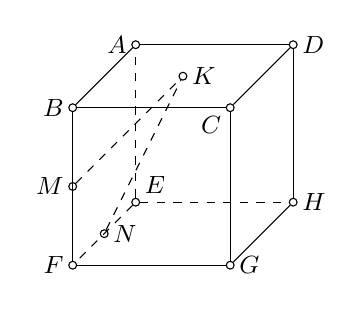
\begin{tikzpicture}
				\begin{scope}
				\small
				\tikzstyle{vnode}=[draw,circle,inner sep =1pt];
				\node[vnode] (v000) at (0,0) {};
				\node[anchor =south west] (t000) at (v000) {$E$};
				\node[vnode] (v001) at (0,2) {$$};
				\node[anchor =east] (t000) at (v001) {$A$};
				\node[vnode] (v011) at (2,2) {$$};
				\node[anchor =west] (t011) at (v011) {$D$};
				\node[vnode] (v010) at (2,0) {$$};
				\node[anchor =west] (t010) at (v010) {$H$};
				\node[vnode] (v100) at (-.8,-.8) {$$};
				\node[anchor =east] (t100) at (v100) {$F$};
				\node[vnode] (v101) at (-.8,1.2) {$$};
				\node[anchor =east] (t101) at (v101) {$B$};
				\node[vnode] (v111) at (1.2,1.2) {$$};
				\node[anchor =north east] (t111) at (v111) {$C$};
				\node[vnode] (v110) at (1.2,-0.8) {$$};
				\node[anchor =west] (t110) at (v110) {$G$};
				\node[vnode] (vK) at (.6,1.6) {$$};
				\node[anchor =west] (tK) at (vK) {$K$};
				\node[vnode] (vM) at (-.8,.2) {$$};
				\node[anchor =east] (tM) at (vM) {$M$};
				\node[vnode] (vN) at (-.4,-.4) {$$};
				\node[anchor =west] (tN) at (vN) {$N$};
				\draw[dashed] (vM) to (vK);
				\draw[dashed] (vN) to (vK);
				\foreach \i in {01,10,11}{
						\draw (v0\i) to (v1\i);
						\draw (v\i  0) to (v\i 1);
				}
				\draw[dashed] (v000) to (v100);
				\draw[dashed] (v000) to (v010);
				\draw[dashed] (v000) to (v001);
				\draw (v001) to (v011);
				\draw (v100) to (v110);
				\draw (v101) to (v111);
				\end{scope}
			\end{tikzpicture}
        \end{QBODY}
        \begin{QFROMS}
        \end{QFROMS}
        \begin{QTAGS}\QTAG{B4C1-2空間向量的坐標表示法}\QTAG{B4C1-4外積、體積與行列式}\QTAG{B4C1空間向量}\end{QTAGS}
        \begin{QANS}
            (2)(3)(4)
        \end{QANS}
        \begin{QSOLLIST}
        \end{QSOLLIST}
        \begin{QEMPTYSPACE}
        \end{QEMPTYSPACE}
    \end{QUESTION}
    \begin{QUESTION}
        \begin{ExamInfo}{98}{學測}{多選}{9}
        \end{ExamInfo}
        \begin{ExamAnsRateInfo}{7}{6}{8}{7}
        \end{ExamAnsRateInfo}
        \begin{QBODY}
            某廠商委託民調機構在甲、乙兩地調查聽過某項產品的居民佔當地居民之百分比(以下簡稱為「知名度」)。結果如下:在 $95\%$ 信心水準之下,該產品在甲、乙兩地的知名度之信賴區間分別為 [ 0.50 , 0.58 ]、[ 0.08 , 0.16 ]。試問下列哪些選項是正確的? 
		\begin{QOPS} 
			\QOP 甲地本次的參訪者中,$54\%$ 的人聽過該產品 
			\QOP 此次民調在乙地的參訪人數少於在甲地的參訪人數 
			\QOP 此次調查結果可解讀為:甲地全體居民中有一半以上的人聽過該產品的機率大於 $95\%$    
			\QOP 若在乙地以同樣方式進行多次民調,所得知名度有 $95\%$ 的機會落在區間 $[0.08 , 0.16 ]$    \QOP 經密集廣告宣傳後,在乙地再次進行民調,並增加參訪人數達原人數的四倍,則在 $95\%$ 
		信心水準之下該產品的知名度之信賴區間寬度會減半(即 0.04)。
		\end{QOPS}
        \end{QBODY}
        \begin{QFROMS}
        \end{QFROMS}
        \begin{QTAGS}\QTAG{B5C1機率與統計}\end{QTAGS}
        \begin{QANS}
            (1)(2)
        \end{QANS}
        \begin{QSOLLIST}
        \end{QSOLLIST}
        \begin{QEMPTYSPACE}
        \end{QEMPTYSPACE}
    \end{QUESTION}
    \begin{QUESTION}
        \begin{ExamInfo}{98}{學測}{多選}{10}
        \end{ExamInfo}
        \begin{ExamAnsRateInfo}{8}{11}{6}{7}
        \end{ExamAnsRateInfo}
        \begin{QBODY}
            設 $a$, $b$, $c$ 為實數,下列有關線性方程組 $\left\{ \begin{array}{rlc}x+2y+az &=&1 \\ 3x+4y+bz &=& -1 \\ 2x+10y+7z &=& c  \end{array}\right.$的敘述哪些是正確的?
			\begin{QOPS} 
				\QOP 若此線性方程組有解,則必定恰有一組解 
				\QOP 若此線性方程組有解,則$11a-3b \neq 7$ 
				\QOP 若此線性方程組有解,則 $c=14$  
				\QOP 若此線性方程組無解,則$11a-3b=7$ 
				\QOP 若此線性方程組無解,則 $c\neq 14$
			\end{QOPS}
        \end{QBODY}
        \begin{QFROMS}
        \end{QFROMS}
        \begin{QTAGS}\QTAG{B4C3矩陣}\QTAG{B4C3-1線性方程組與矩陣}\QTAG{方程組}\end{QTAGS}
        \begin{QANS}
            (4)(5)
        \end{QANS}
        \begin{QSOLLIST}
        \end{QSOLLIST}
        \begin{QEMPTYSPACE}
        \end{QEMPTYSPACE}
    \end{QUESTION}
    \begin{QUESTION}
        \begin{ExamInfo}{98}{學測}{多選}{11}
        \end{ExamInfo}
        \begin{ExamAnsRateInfo}{38}{70}{32}{12}
        \end{ExamAnsRateInfo}
        \begin{QBODY}
            如圖所示,正立方體 $ABCD - EFGH$ 的稜長等於 2 (即 $\overline{AB} = 2$ ), $K$ 為正方形 $ABCD $ 的中心,$M$, $N$ 分別為線段 $\overline{BF}$ ,  $\overline{EF}$ 的中點。試問下列哪些選項是正確的? 
			\begin{QOPS} 
				\QOP  $\lvec{KM} = \frac{1}{2} \lvec{AB} - \frac{1}{2} \lvec{AD} + \frac{1}{2} \lvec{AE}$ 
				\QOP $\lvec{KM} \cdot \lvec{AB}=1$ (3) \quad $\lvec{KM}=3$ 
				\QOP  $\triangle KMN$ 為一直角三角形 
				\QOP $\triangle KMN$ 之面積為 $\frac{\sqrt{10}}{2}$。
			\end{QOPS}
			
			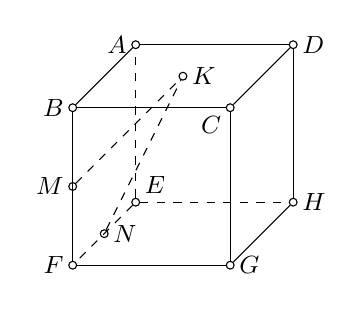
\begin{tikzpicture}
				\begin{scope}
				\small
				\tikzstyle{vnode}=[draw,circle,inner sep =1pt];
				\node[vnode] (v000) at (0,0) {};
				\node[anchor =south west] (t000) at (v000) {$E$};
				\node[vnode] (v001) at (0,2) {$$};
				\node[anchor =east] (t000) at (v001) {$A$};
				\node[vnode] (v011) at (2,2) {$$};
				\node[anchor =west] (t011) at (v011) {$D$};
				\node[vnode] (v010) at (2,0) {$$};
				\node[anchor =west] (t010) at (v010) {$H$};
				\node[vnode] (v100) at (-.8,-.8) {$$};
				\node[anchor =east] (t100) at (v100) {$F$};
				\node[vnode] (v101) at (-.8,1.2) {$$};
				\node[anchor =east] (t101) at (v101) {$B$};
				\node[vnode] (v111) at (1.2,1.2) {$$};
				\node[anchor =north east] (t111) at (v111) {$C$};
				\node[vnode] (v110) at (1.2,-0.8) {$$};
				\node[anchor =west] (t110) at (v110) {$G$};
				\node[vnode] (vK) at (.6,1.6) {$$};
				\node[anchor =west] (tK) at (vK) {$K$};
				\node[vnode] (vM) at (-.8,.2) {$$};
				\node[anchor =east] (tM) at (vM) {$M$};
				\node[vnode] (vN) at (-.4,-.4) {$$};
				\node[anchor =west] (tN) at (vN) {$N$};
				\draw[dashed] (vM) to (vK);
				\draw[dashed] (vN) to (vK);
				\foreach \i in {01,10,11}{
						\draw (v0\i) to (v1\i);
						\draw (v\i  0) to (v\i 1);
				}
				\draw[dashed] (v000) to (v100);
				\draw[dashed] (v000) to (v010);
				\draw[dashed] (v000) to (v001);
				\draw (v001) to (v011);
				\draw (v100) to (v110);
				\draw (v101) to (v111);
				\end{scope}
			\end{tikzpicture}
        \end{QBODY}
        \begin{QFROMS}
        \end{QFROMS}
        \begin{QTAGS}\QTAG{B4C1-3空間向量的內積}\QTAG{B4C1空間向量}\end{QTAGS}
        \begin{QANS}
            (1)(4)
        \end{QANS}
        \begin{QSOLLIST}
        \end{QSOLLIST}
        \begin{QEMPTYSPACE}
        \end{QEMPTYSPACE}
    \end{QUESTION}
\end{QUESTIONS}
\begin{QUESTIONS}
    \begin{QUESTION}
        \begin{ExamInfo}{98}{學測}{填充}{A}
        \end{ExamInfo}
        \begin{ExamAnsRateInfo}{76}{92}{86}{50}
        \end{ExamAnsRateInfo}
        \begin{QBODY}
            從 1 到 100 的正整數中刪去所有的質數、2 的倍數及 3 的倍數之後,剩下最大的數為 $\TCNBOX{\TCN\TCN}$ 。
        \end{QBODY}
        \begin{QFROMS}
        \end{QFROMS}
        \begin{QTAGS}\QTAG{集合}\QTAG{乘法原理加法原理}\QTAG{B2C2-1簡單的邏輯與集合}\QTAG{B2C2排列組合}\end{QTAGS}
        \begin{QANS}
            $95$
        \end{QANS}
        \begin{QSOLLIST}
        \end{QSOLLIST}
        \begin{QEMPTYSPACE}
        \end{QEMPTYSPACE}
    \end{QUESTION}
    \begin{QUESTION}
        \begin{ExamInfo}{98}{學測}{填充}{B}
        \end{ExamInfo}
        \begin{ExamAnsRateInfo}{31}{69}{22}{2}
        \end{ExamAnsRateInfo}
        \begin{QBODY}
            坐標平面上有四點 $O(0,0)$, $A(-3,-5)$, $B(6,0)$, $C(x,y)$。今有一質點在 $O$ 點沿 $\lvec{AO}$ 方向前進 $\lvec{AO}$ 距離後停在 $P$,再沿 $\lvec{BP}$ 方向前進 $2\overline{BP}$ 距離後停在 $Q$。 假設此質點繼續沿 $\lvec{CQ}$ 方向前進 $3\overline{CQ}$ 距離後回到原點 $O$,則 $(x,y)=\TCNBOX{\TCN\TCN,\TCN\TCN}$ 。
        \end{QBODY}
        \begin{QFROMS}
        \end{QFROMS}
        \begin{QTAGS}\QTAG{線性組合}\QTAG{B3C3-2平面向量的內積}\QTAG{B3C3平面向量}\QTAG{距離}\end{QTAGS}
        \begin{QANS}
            $(-4,20)$
        \end{QANS}
        \begin{QSOLLIST}
        \end{QSOLLIST}
        \begin{QEMPTYSPACE}
        \end{QEMPTYSPACE}
    \end{QUESTION}
    \begin{QUESTION}
        \begin{ExamInfo}{98}{學測}{填充}{C}
        \end{ExamInfo}
        \begin{ExamAnsRateInfo}{60}{92}{69}{19}
        \end{ExamAnsRateInfo}
        \begin{QBODY}
            抽獎遊戲中,參加者自箱中抽出一球,確定顏色後放回。只有抽得藍色或紅色球者可得消費劵,其金額分別為(抽得藍色球者)2000 元、(抽得紅色球者)1000 元。箱中已置有 2 顆藍色球及 5 顆 紅色球。在抽出任一球之機率相等的條件下,主辦單位希望參加者所得消費劵金額的期望值為 300 元,則主辦單位應於箱內再置入 $\TCNBOX{\TCN\TCN}$ 顆其他顏色的球。
        \end{QBODY}
        \begin{QFROMS}
        \end{QFROMS}
        \begin{QTAGS}\QTAG{B5C1機率與統計}\end{QTAGS}
        \begin{QANS}
            $23$
        \end{QANS}
        \begin{QSOLLIST}
        \end{QSOLLIST}
        \begin{QEMPTYSPACE}
        \end{QEMPTYSPACE}
    \end{QUESTION}
    \begin{QUESTION}
        \begin{ExamInfo}{98}{學測}{填充}{D}
        \end{ExamInfo}
        \begin{ExamAnsRateInfo}{39}{79}{32}{6}
        \end{ExamAnsRateInfo}
        \begin{QBODY}
            坐標平面上有兩條平行直線。它們的 $x$ 截距相差 $20$, $y$ 截距相差 $15$。則這兩條平行直線的距離為 $\TCNBOX{\TCN\TCN}$ 。
        \end{QBODY}
        \begin{QFROMS}
        \end{QFROMS}
        \begin{QTAGS}\QTAG{B3C2-1直線方程式及其圖形}\QTAG{B3C2直線與圓}\end{QTAGS}
        \begin{QANS}
            $12$
        \end{QANS}
        \begin{QSOLLIST}
        \end{QSOLLIST}
        \begin{QEMPTYSPACE}
        \end{QEMPTYSPACE}
    \end{QUESTION}
    \begin{QUESTION}
        \begin{ExamInfo}{98}{學測}{填充}{E}
        \end{ExamInfo}
        \begin{ExamAnsRateInfo}{13}{33}{6}{0}
        \end{ExamAnsRateInfo}
        \begin{QBODY}
            假設 $\Gamma_1$ 為坐標平面上一開口向上的拋物線,其對稱軸為 $x=-\frac{3}{4}$ 且焦距(焦點到頂點的距離) 為 $\frac{1}{8}$。若 $\Gamma_1$ 與另一拋物線 $\Gamma_2 :y=x^2$ 恰交於一點,則 $\Gamma_1$ 的頂點之 $y$ 坐標為$\TCNBOX{\FR{\TCN}{\TCN}}$。(化成最簡分數)
        \end{QBODY}
        \begin{QFROMS}
        \end{QFROMS}
        \begin{QTAGS}\QTAG{B4C4二次曲線}\QTAG{B4C4-1拋物線}\QTAG{圖形}\end{QTAGS}
        \begin{QANS}
            $\dfrac{9}{8}$
        \end{QANS}
        \begin{QSOLLIST}
        \end{QSOLLIST}
        \begin{QEMPTYSPACE}
        \end{QEMPTYSPACE}
    \end{QUESTION}
    \begin{QUESTION}
        \begin{ExamInfo}{98}{學測}{填充}{F}
        \end{ExamInfo}
        \begin{ExamAnsRateInfo}{6}{15}{2}{1}
        \end{ExamAnsRateInfo}
        \begin{QBODY}
            某公司為了響應節能減碳政策, 決定在五年後將公司該年二氧化碳排放量降為目前排放量的 $75 \%$。 公司希望每年依固定的比率(當年和前一年排放量的比) 逐年減少二氧化碳的排放量。 若要達到這項目標,則該公司每年至少要比前一年減少 $\TCNBOX{\TCN.\TCN} \%$ 的二氧化碳的排放量。 (計算到小數點後第一位, 以下四捨五入。)
        \end{QBODY}
        \begin{QFROMS}
        \end{QFROMS}
        \begin{QTAGS}\QTAG{應用問題}\QTAG{B1C3指對數函數}\QTAG{B1C3-5指數與對數的應用}\end{QTAGS}
        \begin{QANS}
            $5.6$
        \end{QANS}
        \begin{QSOLLIST}
        \end{QSOLLIST}
        \begin{QEMPTYSPACE}
        \end{QEMPTYSPACE}
    \end{QUESTION}
    \begin{QUESTION}
        \begin{ExamInfo}{98}{學測}{填充}{G}
        \end{ExamInfo}
        \begin{ExamAnsRateInfo}{36}{80}{26}{2}
        \end{ExamAnsRateInfo}
        \begin{QBODY}
            坐標空間中 $xy$ 平面上有一正方形,其頂點為 $O(0,0,0)$, $A(8,0,0)$, $B(8,8,0)$, $C(0,8,0)$。另一點 $P$ 在 $xy$ 平面的上方,且與 $O$, $A$, $B$, $C$ 四點的距離皆等於 $6$。若 $x + by + cz = d$ 為通過 $A$, $B$, $P$ 三點的平面,則 $(b,c,d)=\TCNBOX{\TCN,\TCN,\TCN}$。
        \end{QBODY}
        \begin{QFROMS}
        \end{QFROMS}
        \begin{QTAGS}\QTAG{B4C2空間中的平面與直線}\QTAG{B4C2-1平面方程式}\QTAG{距離}\end{QTAGS}
        \begin{QANS}
            $(0,2,8)$
        \end{QANS}
        \begin{QSOLLIST}
        \end{QSOLLIST}
        \begin{QEMPTYSPACE}
        \end{QEMPTYSPACE}
    \end{QUESTION}
    \begin{QUESTION}
        \begin{ExamInfo}{98}{學測}{填充}{H}
        \end{ExamInfo}
        \begin{ExamAnsRateInfo}{36}{57}{36}{15}
        \end{ExamAnsRateInfo}
        \begin{QBODY}
            有一橢圓與一雙曲線有共同的焦點 $F_1$ 、 $F_2$ ,且雙曲線的貫軸長和橢圓的短軸長相等。設 $P$ 為此橢圓與雙曲線的一個交點,且 $\overline{PF_1} \times \overline{PF}_2 =64$ ,則 $\overline{F_1F_2} =$ 
$\TCNBOX{\TCN\TCN}$。
        \end{QBODY}
        \begin{QFROMS}
        \end{QFROMS}
        \begin{QTAGS}\QTAG{B4C4-3雙曲線}\QTAG{B4C4二次曲線}\QTAG{B4C4-2橢圓}\QTAG{圖形}\end{QTAGS}
        \begin{QANS}
            $16$
        \end{QANS}
        \begin{QSOLLIST}
        \end{QSOLLIST}
        \begin{QEMPTYSPACE}
        \end{QEMPTYSPACE}
    \end{QUESTION}
    \begin{QUESTION}
        \begin{ExamInfo}{98}{學測}{填充}{I}
        \end{ExamInfo}
        \begin{ExamAnsRateInfo}{11}{27}{5}{1}
        \end{ExamAnsRateInfo}
        \begin{QBODY}
            在 $\triangle ABC$ 中, $\overline{AB}=10$,$\overline{AC}=9$, $\cos \angle{BAC}= \frac{3}{8}$。設點 $P$, $Q$ 分別在邊 $AB$, $AC$上使得 $\triangle APQ$之面積為 $\triangle ABC$ 面積之一半,則 $\overline{PQ}$ 之最小可能值為 
			$\TCNBOX{\FR{\TCN\TCN}{\TCN}}$。
        \end{QBODY}
        \begin{QFROMS}
        \end{QFROMS}
        \begin{QTAGS}\QTAG{面積}\QTAG{餘弦定理}\QTAG{B3C1-3正弦定理與餘弦定理}\QTAG{B3C1三角}\end{QTAGS}
        \begin{QANS}
            $\FR{15}{2}$
        \end{QANS}
        \begin{QSOLLIST}
        \end{QSOLLIST}
        \begin{QEMPTYSPACE}
        \end{QEMPTYSPACE}
    \end{QUESTION}
\end{QUESTIONS}

% !TEX encoding = UTF-8 Unicode
% !TEX TS-program = xelatex 
\begin{QUESTIONS}
    \begin{QUESTION}
        \begin{ExamInfo}{099}{學測}{單選}{1}
        \end{ExamInfo}
        \begin{ExamAnsRateInfo}{49}{82}{49}{16}
        \end{ExamAnsRateInfo}
        \begin{QBODY}
        \end{QBODY}
        \begin{QFROMS}
        \end{QFROMS}
        \begin{QTAGS}\QTAG{B2C2排列組合}\end{QTAGS}
        \begin{QANS}
            (2)
        \end{QANS}
        \begin{QSOLLIST}
        \end{QSOLLIST}
        \begin{QEMPTYSPACE}
        \end{QEMPTYSPACE}
    \end{QUESTION}
    \begin{QUESTION}
        \begin{ExamInfo}{099}{學測}{單選}{2}
        \end{ExamInfo}
        \begin{ExamAnsRateInfo}{58}{83}{62}{29}
        \end{ExamAnsRateInfo}
        \begin{QBODY}
        \end{QBODY}
        \begin{QFROMS}
        \end{QFROMS}
        \begin{QTAGS}\QTAG{B3C3平面向量}\end{QTAGS}
        \begin{QANS}
            (3)
        \end{QANS}
        \begin{QSOLLIST}
        \end{QSOLLIST}
        \begin{QEMPTYSPACE}
        \end{QEMPTYSPACE}
    \end{QUESTION}
    \begin{QUESTION}
        \begin{ExamInfo}{099}{學測}{單選}{3}
        \end{ExamInfo}
        \begin{ExamAnsRateInfo}{55}{84}{62}{19}
        \end{ExamAnsRateInfo}
        \begin{QBODY}
        \end{QBODY}
        \begin{QFROMS}
        \end{QFROMS}
        \begin{QTAGS}\QTAG{B5C1機率與統計}\end{QTAGS}
        \begin{QANS}
            (5)
        \end{QANS}
        \begin{QSOLLIST}
        \end{QSOLLIST}
        \begin{QEMPTYSPACE}
        \end{QEMPTYSPACE}
    \end{QUESTION}
    \begin{QUESTION}
        \begin{ExamInfo}{099}{學測}{單選}{4}
        \end{ExamInfo}
        \begin{ExamAnsRateInfo}{33}{61}{25}{13}
        \end{ExamAnsRateInfo}
        \begin{QBODY}
        \end{QBODY}
        \begin{QFROMS}
        \end{QFROMS}
        \begin{QTAGS}\QTAG{B3C1三角}\end{QTAGS}
        \begin{QANS}
            (1)
        \end{QANS}
        \begin{QSOLLIST}
        \end{QSOLLIST}
        \begin{QEMPTYSPACE}
        \end{QEMPTYSPACE}
    \end{QUESTION}
    \begin{QUESTION}
        \begin{ExamInfo}{099}{學測}{單選}{5}
        \end{ExamInfo}
        \begin{ExamAnsRateInfo}{26}{46}{20}{12}
        \end{ExamAnsRateInfo}
        \begin{QBODY}
        \end{QBODY}
        \begin{QFROMS}
        \end{QFROMS}
        \begin{QTAGS}\QTAG{B1C3指對數函數}\end{QTAGS}
        \begin{QANS}
            (3)
        \end{QANS}
        \begin{QSOLLIST}
        \end{QSOLLIST}
        \begin{QEMPTYSPACE}
        \end{QEMPTYSPACE}
    \end{QUESTION}
    \begin{QUESTION}
        \begin{ExamInfo}{099}{學測}{單選}{6}
        \end{ExamInfo}
        \begin{ExamAnsRateInfo}{49}{70}{53}{24}
        \end{ExamAnsRateInfo}
        \begin{QBODY}
        \end{QBODY}
        \begin{QFROMS}
        \end{QFROMS}
        \begin{QTAGS}\QTAG{B4C1空間向量}\end{QTAGS}
        \begin{QANS}
            (4)
        \end{QANS}
        \begin{QSOLLIST}
        \end{QSOLLIST}
        \begin{QEMPTYSPACE}
        \end{QEMPTYSPACE}
    \end{QUESTION}
    \begin{QUESTION}
        \begin{ExamInfo}{099}{學測}{單選}{7}
        \end{ExamInfo}
        \begin{ExamAnsRateInfo}{33}{65}{22}{12}
        \end{ExamAnsRateInfo}
        \begin{QBODY}
        \end{QBODY}
        \begin{QFROMS}
        \end{QFROMS}
        \begin{QTAGS}\QTAG{B4C4二次曲線}\end{QTAGS}
        \begin{QANS}
            (4)
        \end{QANS}
        \begin{QSOLLIST}
        \end{QSOLLIST}
        \begin{QEMPTYSPACE}
        \end{QEMPTYSPACE}
    \end{QUESTION}
\end{QUESTIONS}
\begin{QUESTIONS}
    \begin{QUESTION}
        \begin{ExamInfo}{099}{學測}{多選}{8}
        \end{ExamInfo}
        \begin{ExamAnsRateInfo}{39}{72}{29}{16}
        \end{ExamAnsRateInfo}
        \begin{QBODY}
        \end{QBODY}
        \begin{QFROMS}
        \end{QFROMS}
        \begin{QTAGS}\QTAG{B3C1三角}\end{QTAGS}
        \begin{QANS}
            (2)(3)
        \end{QANS}
        \begin{QSOLLIST}
        \end{QSOLLIST}
        \begin{QEMPTYSPACE}
        \end{QEMPTYSPACE}
    \end{QUESTION}
    \begin{QUESTION}
        \begin{ExamInfo}{099}{學測}{多選}{9}
        \end{ExamInfo}
        \begin{ExamAnsRateInfo}{24}{50}{14}{8}
        \end{ExamAnsRateInfo}
        \begin{QBODY}
        \end{QBODY}
        \begin{QFROMS}
        \end{QFROMS}
        \begin{QTAGS}\QTAG{綜合}\end{QTAGS}
        \begin{QANS}
            (1)(5)
        \end{QANS}
        \begin{QSOLLIST}
        \end{QSOLLIST}
        \begin{QEMPTYSPACE}
        \end{QEMPTYSPACE}
    \end{QUESTION}
    \begin{QUESTION}
        \begin{ExamInfo}{099}{學測}{多選}{10}
        \end{ExamInfo}
        \begin{ExamAnsRateInfo}{34}{53}{33}{16}
        \end{ExamAnsRateInfo}
        \begin{QBODY}
        \end{QBODY}
        \begin{QFROMS}
        \end{QFROMS}
        \begin{QTAGS}\QTAG{B2C1數列級數}\end{QTAGS}
        \begin{QANS}
            (2)(3)(4)
        \end{QANS}
        \begin{QSOLLIST}
        \end{QSOLLIST}
        \begin{QEMPTYSPACE}
        \end{QEMPTYSPACE}
    \end{QUESTION}
    \begin{QUESTION}
        \begin{ExamInfo}{099}{學測}{多選}{11}
        \end{ExamInfo}
        \begin{ExamAnsRateInfo}{17}{25}{16}{10}
        \end{ExamAnsRateInfo}
        \begin{QBODY}
        \end{QBODY}
        \begin{QFROMS}
        \end{QFROMS}
        \begin{QTAGS}\QTAG{B4C1空間向量}\end{QTAGS}
        \begin{QANS}
            (1)(3)(5)
        \end{QANS}
        \begin{QSOLLIST}
        \end{QSOLLIST}
        \begin{QEMPTYSPACE}
        \end{QEMPTYSPACE}
    \end{QUESTION}
    \begin{QUESTION}
        \begin{ExamInfo}{099}{學測}{多選}{12}
        \end{ExamInfo}
        \begin{ExamAnsRateInfo}{21}{37}{16}{10}
        \end{ExamAnsRateInfo}
        \begin{QBODY}
        \end{QBODY}
        \begin{QFROMS}
        \end{QFROMS}
        \begin{QTAGS}\QTAG{B5C1機率與統計}\end{QTAGS}
        \begin{QANS}
            (2)(4)
        \end{QANS}
        \begin{QSOLLIST}
        \end{QSOLLIST}
        \begin{QEMPTYSPACE}
        \end{QEMPTYSPACE}
    \end{QUESTION}
\end{QUESTIONS}
\begin{QUESTIONS}
    \begin{QUESTION}
        \begin{ExamInfo}{099}{學測}{填充}{A}
        \end{ExamInfo}
        \begin{ExamAnsRateInfo}{29}{64}{19}{4}
        \end{ExamAnsRateInfo}
        \begin{QBODY}
        \end{QBODY}
        \begin{QFROMS}
        \end{QFROMS}
        \begin{QTAGS}\QTAG{B3C3平面向量}\end{QTAGS}
        \begin{QANS}
            $(6,8)$
        \end{QANS}
        \begin{QSOLLIST}
        \end{QSOLLIST}
        \begin{QEMPTYSPACE}
        \end{QEMPTYSPACE}
    \end{QUESTION}
    \begin{QUESTION}
        \begin{ExamInfo}{099}{學測}{填充}{B}
        \end{ExamInfo}
        \begin{ExamAnsRateInfo}{29}{71}{15}{1}
        \end{ExamAnsRateInfo}
        \begin{QBODY}
        \end{QBODY}
        \begin{QFROMS}
        \end{QFROMS}
        \begin{QTAGS}\QTAG{B1C2多項式函數}\end{QTAGS}
        \begin{QANS}
            $-65$
        \end{QANS}
        \begin{QSOLLIST}
        \end{QSOLLIST}
        \begin{QEMPTYSPACE}
        \end{QEMPTYSPACE}
    \end{QUESTION}
    \begin{QUESTION}
        \begin{ExamInfo}{099}{學測}{填充}{C}
        \end{ExamInfo}
        \begin{ExamAnsRateInfo}{26}{53}{22}{3}
        \end{ExamAnsRateInfo}
        \begin{QBODY}
        \end{QBODY}
        \begin{QFROMS}
        \end{QFROMS}
        \begin{QTAGS}\QTAG{B2C2排列組合}\end{QTAGS}
        \begin{QANS}
            $432$
        \end{QANS}
        \begin{QSOLLIST}
        \end{QSOLLIST}
        \begin{QEMPTYSPACE}
        \end{QEMPTYSPACE}
    \end{QUESTION}
    \begin{QUESTION}
        \begin{ExamInfo}{099}{學測}{填充}{D}
        \end{ExamInfo}
        \begin{ExamAnsRateInfo}{41}{71}{42}{10}
        \end{ExamAnsRateInfo}
        \begin{QBODY}
        \end{QBODY}
        \begin{QFROMS}
        \end{QFROMS}
        \begin{QTAGS}\QTAG{B4C3矩陣}\end{QTAGS}
        \begin{QANS}
            $14$
        \end{QANS}
        \begin{QSOLLIST}
        \end{QSOLLIST}
        \begin{QEMPTYSPACE}
        \end{QEMPTYSPACE}
    \end{QUESTION}
    \begin{QUESTION}
        \begin{ExamInfo}{099}{學測}{填充}{E}
        \end{ExamInfo}
        \begin{ExamAnsRateInfo}{31}{75}{17}{1}
        \end{ExamAnsRateInfo}
        \begin{QBODY}
        \end{QBODY}
        \begin{QFROMS}
        \end{QFROMS}
        \begin{QTAGS}\QTAG{B3C1三角}\end{QTAGS}
        \begin{QANS}
            $\dfrac{90}{7}$
        \end{QANS}
        \begin{QSOLLIST}
        \end{QSOLLIST}
        \begin{QEMPTYSPACE}
        \end{QEMPTYSPACE}
    \end{QUESTION}
    \begin{QUESTION}
        \begin{ExamInfo}{099}{學測}{填充}{F}
        \end{ExamInfo}
        \begin{ExamAnsRateInfo}{15}{40}{4}{1}
        \end{ExamAnsRateInfo}
        \begin{QBODY}
        \end{QBODY}
        \begin{QFROMS}
        \end{QFROMS}
        \begin{QTAGS}\QTAG{B1C2多項式函數}\end{QTAGS}
        \begin{QANS}
            $\sqrt{41}$
        \end{QANS}
        \begin{QSOLLIST}
        \end{QSOLLIST}
        \begin{QEMPTYSPACE}
        \end{QEMPTYSPACE}
    \end{QUESTION}
    \begin{QUESTION}
        \begin{ExamInfo}{099}{學測}{填充}{G}
        \end{ExamInfo}
        \begin{ExamAnsRateInfo}{25}{58}{14}{3}
        \end{ExamAnsRateInfo}
        \begin{QBODY}
        \end{QBODY}
        \begin{QFROMS}
        \end{QFROMS}
        \begin{QTAGS}\QTAG{B3C1三角}\end{QTAGS}
        \begin{QANS}
            $\frac{5}{2}$
        \end{QANS}
        \begin{QSOLLIST}
        \end{QSOLLIST}
        \begin{QEMPTYSPACE}
        \end{QEMPTYSPACE}
    \end{QUESTION}
    \begin{QUESTION}
        \begin{ExamInfo}{099}{學測}{填充}{H}
        \end{ExamInfo}
        \begin{ExamAnsRateInfo}{10}{27}{2}{1}
        \end{ExamAnsRateInfo}
        \begin{QBODY}
        \end{QBODY}
        \begin{QFROMS}
        \end{QFROMS}
        \begin{QTAGS}\QTAG{B4C4二次曲線}\end{QTAGS}
        \begin{QANS}
            $\frac{21}{4}$
        \end{QANS}
        \begin{QSOLLIST}
        \end{QSOLLIST}
        \begin{QEMPTYSPACE}
        \end{QEMPTYSPACE}
    \end{QUESTION}
\end{QUESTIONS}

% !TEX encoding = UTF-8 Unicode
% !TEX TS-program = xelatex 
\begin{QUESTIONS}
    \begin{QUESTION}
        \begin{ExamInfo}{100}{學測}{單選}{1}
        \end{ExamInfo}
        \begin{ExamAnsRateInfo}{85}{99}{98}{58}
        \end{ExamAnsRateInfo}
        \begin{QBODY}
			有一箱子,內有 3 黑球與 2 白球。有一遊戲,從箱子中任取出一球。假設每一顆球被取出的機率都相同,若取出黑球可得獎金 50 元,而取出白球可得獎金 100 元,則下 列哪一個選項是此遊戲的獎金期望值?
			\begin{QOPS} 
				\QOP 70 元
				\QOP 75 元 
				\QOP 80 元 
				\QOP 85 元 
				\QOP 90 元
			\end{QOPS}
        \end{QBODY}
        \begin{QFROMS}
        \end{QFROMS}
        \begin{QTAGS}\QTAG{B5C1機率與統計}\end{QTAGS}
        \begin{QANS}
            (1)
        \end{QANS}
        \begin{QSOLLIST}
        \end{QSOLLIST}
        \begin{QEMPTYSPACE}
        \end{QEMPTYSPACE}
    \end{QUESTION}
    \begin{QUESTION}
        \begin{ExamInfo}{100}{學測}{單選}{2}
        \end{ExamInfo}
        \begin{ExamAnsRateInfo}{72}{92}{82}{42}
        \end{ExamAnsRateInfo}
        \begin{QBODY}
			多項式 $4(x^2 +1)+(x+1)^2(x-3)+(x-1)^3$ 等於下列哪一個選項? 
			\begin{QOPS} 
				\QOP $x(x+1)^2$ 
				\QOP $2x(x-1)^2$
				\QOP $x(x-1)(x+1)$    
				\QOP  $2(x-1)^2(x+1)$    
				\QOP $2x(x-1)(x+1)$
			\end{QOPS}
        \end{QBODY}
        \begin{QFROMS}
        \end{QFROMS}
        \begin{QTAGS}\QTAG{B1C2多項式函數}\end{QTAGS}
        \begin{QANS}
            (5)
        \end{QANS}
        \begin{QSOLLIST}
        \end{QSOLLIST}
        \begin{QEMPTYSPACE}
        \end{QEMPTYSPACE}
    \end{QUESTION}
    \begin{QUESTION}
        \begin{ExamInfo}{100}{學測}{單選}{3}
        \end{ExamInfo}
        \begin{ExamAnsRateInfo}{28}{56}{14}{14}
        \end{ExamAnsRateInfo}
        \begin{QBODY}
			設 $(a_{n+1})^2=\frac{1}{\sqrt{10}}(a_n)^2$,$n$ 為正整數,且知 $a_n $ 皆為正。令 $b_n=\log a_n$,則數列 $b_1, b_2,b_3,\cdots,$ 為 
			\begin{QOPS} 
				\QOP 公差為正的等差數列 
				\QOP 公差為負的等差數列 
				\QOP 公比為正的等比數列 
				\QOP 公比為負的等比數列 
				\QOP 既非等差亦非等比數列 。
			\end{QOPS}
        \end{QBODY}
        \begin{QFROMS}
        \end{QFROMS}
        \begin{QTAGS}\QTAG{B1C3指對數函數}\end{QTAGS}
        \begin{QANS}
            (2)
        \end{QANS}
        \begin{QSOLLIST}
        \end{QSOLLIST}
        \begin{QEMPTYSPACE}
        \end{QEMPTYSPACE}
    \end{QUESTION}
    \begin{QUESTION}
        \begin{ExamInfo}{100}{學測}{單選}{4}
        \end{ExamInfo}
        \begin{ExamAnsRateInfo}{30}{51}{20}{19}
        \end{ExamAnsRateInfo}
        \begin{QBODY}
			坐標平面上滿足方程式 $(\frac{x^2}{5^2} + \frac{y^2}{4^2})(\frac{x^2}{3^2} - \frac{y^2}{4^2})=0$ 的點 $(x,y)$ 所構成的圖形為 \quad 
			\begin{QOPS} 
                \QOP 只有原點 
				\QOP 橢圓及原點 
				\QOP 兩條相異直線 
				\QOP 橢圓及雙曲線 
				\QOP 雙曲線及原點
			\end{QOPS}
        \end{QBODY}
        \begin{QFROMS}
        \end{QFROMS}
        \begin{QTAGS}\QTAG{B4C4二次曲線}\end{QTAGS}
        \begin{QANS}
            (3)
        \end{QANS}
        \begin{QSOLLIST}
        \end{QSOLLIST}
        \begin{QEMPTYSPACE}
        \end{QEMPTYSPACE}
    \end{QUESTION}
    \begin{QUESTION}
        \begin{ExamInfo}{100}{學測}{單選}{5}
        \end{ExamInfo}
        \begin{ExamAnsRateInfo}{67}{94}{77}{30}
        \end{ExamAnsRateInfo}
        \begin{QBODY}
		請問下面哪一個選項是正確的? 
		\begin{QOPS} 
			\QOP $3^7 < 7^3$ 
			\QOP $5^{10} < 10^{5}$ 
			\QOP $2^{100} < 10^{30}$ 
			\QOP $\log_2{3} = 1.5$ 
			\QOP $\log_2{11} < 3.5$ 。
		\end{QOPS}
        \end{QBODY}
        \begin{QFROMS}
        \end{QFROMS}
        \begin{QTAGS}\QTAG{B1C3指對數函數}\end{QTAGS}
        \begin{QANS}
            (5)
        \end{QANS}
        \begin{QSOLLIST}
        \end{QSOLLIST}
        \begin{QEMPTYSPACE}
        \end{QEMPTYSPACE}
    \end{QUESTION}
    \begin{QUESTION}
        \begin{ExamInfo}{100}{學測}{單選}{6}
        \end{ExamInfo}
        \begin{ExamAnsRateInfo}{69}{91}{76}{40}
        \end{ExamAnsRateInfo}
        \begin{QBODY}
		根據台灣壽險業的資料,男性從 0 歲、1 歲、...到 60 歲各年齡層的死亡率(單位:$\%$)
		依序為
		1.0250, 0.2350, 0.1520, 0.1010, 0.0720, 0.0590, 0.0550, 0.0540, 0.0540, 0.0520, 0.0490, 0.0470, 0.0490, 0.0560, 0.0759, 0.1029, 0.1394, 0.1890, 0.2034, 0.2123, 0.2164, 0.2166, 0.2137, 0.2085, 0.2019, 0.1948, 0.1882, 0.1830, 0.1799, 0.1793, 0.1813, 0.1862, 0.1941, 0.2051, 0.2190, 0.2354, 0.2539, 0.2742, 0.2961, 0.3202, 0.3472, 0.3779, 0.4129, 0.4527, 0.4962, 0.5420, 0.5886, 0.6346, 0.6791, 0.7239, 0.7711, 0.8229, 0.8817, 0.9493, 1.0268, 1.1148, 1.2139, 1.3250, 1.4485, 1.5851, 1.7353。
		經初步整理後,已知 61 個資料中共有 24 個資料小於 0.2。請問死亡率資料的中位數為下列哪一個選項?
			\begin{QOPS}
				\QOP 0.2034
				\QOP 0.2164
				\QOP 0.2137
				\QOP 0.2085 
				\QOP 0.2019
			\end{QOPS}
        \end{QBODY}
        \begin{QFROMS}
        \end{QFROMS}
        \begin{QTAGS}\QTAG{B2C4數據分析}\end{QTAGS}
        \begin{QANS}
            (2)
        \end{QANS}
        \begin{QSOLLIST}
        \end{QSOLLIST}
        \begin{QEMPTYSPACE}
        \end{QEMPTYSPACE}
    \end{QUESTION}
\end{QUESTIONS}
\begin{QUESTIONS}
    \begin{QUESTION}
        \begin{ExamInfo}{100}{學測}{多選}{7}
        \end{ExamInfo}
        \begin{ExamAnsRateInfo}{40}{73}{32}{15}
        \end{ExamAnsRateInfo}
        \begin{QBODY}
			設 $O$、$A$、$B$ 分別為複數平面上代表 $0$、$1+i$、以及 $1-i$ 的點。請問下列哪些選項所對應的點落在 $\triangle OAB$ 的內部?
			\begin{QOPS} 
				\QOP $\cos 60^\circ$    
				\QOP $\cos 50^\circ +i \sin 50^\circ$    \QOP $\frac{4-3i}{5}$    
				\QOP $\frac{1+\sqrt{3}i}{2}$  
				\QOP $(\cos30^\circ +i\sin 30^\circ) ^{25}$
			\end{QOPS}
        \end{QBODY}
        \begin{QFROMS}
        \end{QFROMS}
        \begin{QTAGS}\QTAG{B5C2三角函數II}\end{QTAGS}
        \begin{QANS}
            (1)(3)(5)
        \end{QANS}
        \begin{QSOLLIST}
        \end{QSOLLIST}
        \begin{QEMPTYSPACE}
        \end{QEMPTYSPACE}
    \end{QUESTION}
    \begin{QUESTION}
        \begin{ExamInfo}{100}{學測}{多選}{8}
        \end{ExamInfo}
        \begin{ExamAnsRateInfo}{54}{82}{55}{25}
        \end{ExamAnsRateInfo}
        \begin{QBODY}
			已知 $\sin \theta = -\frac{2}{3}$ 且 $\cos\theta >0$,請問下列哪些選項是正確的? 
			\begin{QOPS} 
				\QOP $\tan \theta < 0$  
				\QOP $\tan^2\theta > \frac{4}{9}$ 
				\QOP $ \sin^2 \theta > \cos^2 \theta$ 
				\QOP $\sin 2\theta>0$ 
				\QOP 標準位置角 $\theta$ 與 $2\theta$的終邊位在不同的象限
			\end{QOPS}
        \end{QBODY}
        \begin{QFROMS}
        \end{QFROMS}
        \begin{QTAGS}\QTAG{B3C1三角}\end{QTAGS}
        \begin{QANS}
            (1)(2)
        \end{QANS}
        \begin{QSOLLIST}
        \end{QSOLLIST}
        \begin{QEMPTYSPACE}
        \end{QEMPTYSPACE}
    \end{QUESTION}
    \begin{QUESTION}
        \begin{ExamInfo}{100}{學測}{多選}{9}
        \end{ExamInfo}
        \begin{ExamAnsRateInfo}{61}{90}{62}{31}
        \end{ExamAnsRateInfo}
        \begin{QBODY}
			考慮坐標平面上以 $O(0,0)$、$A(3,0)$、$B(0,4)$ 為頂點的三角形,令 $C_1$、$C_2$ 分別為 $\triangle OAB$ 的外接圓、內切圓。請問下列哪些選項是正確的?
			\begin{QOPS}
				\QOP $C_1$ 的半徑為2 
				\QOP $C_1$ 的圓心在直線 $y=x$ 上 
				\QOP $C_1$ 的圓心在直線 $4x+3y=12$ 上    
				\QOP $C_2$ 的圓心在直線 $y=x$ 上 \quad 
				\QOP $C_2$ 的圓心在直線 $4x+3y=6$ 上
			\end{QOPS}
        \end{QBODY}
        \begin{QFROMS}
        \end{QFROMS}
        \begin{QTAGS}\QTAG{B3C2直線與圓}\end{QTAGS}
        \begin{QANS}
            (3)(4)
        \end{QANS}
        \begin{QSOLLIST}
        \end{QSOLLIST}
        \begin{QEMPTYSPACE}
        \end{QEMPTYSPACE}
    \end{QUESTION}
    \begin{QUESTION}
        \begin{ExamInfo}{100}{學測}{多選}{10}
        \end{ExamInfo}
        \begin{ExamAnsRateInfo}{37}{64}{33}{14}
        \end{ExamAnsRateInfo}
        \begin{QBODY}
			坐標平面中,向量 $\lvec{w}$ 與向量 $\lvec{v} = (2,\sqrt{5})$ 互相垂直且等長。請問下列哪些選項是正確的?
			\begin{QOPS} 
				\QOP 向量 $\lvec{w}$ 必為 $(\sqrt{5},-2)$ 或 $(-\sqrt{5},2)$ 
				\QOP 向量$\lvec{v}+\lvec{w}$ 與 $\lvec{v}-\lvec{w}$ 等長 
				\QOP 向量 $\lvec{v}+\lvec{w}$ 與 $\lvec{w}$ 的夾角可能為 $135^\circ$ 
				\QOP 若向量 $\lvec{u}=a \lvec{v}+b \lvec{w}$,其中 $a,b$ 為實數,則向量 $\lvec{u}$ 的長度為 $\sqrt{a^2 +b^2}$ 
				\QOP 若向量 $(1,0)=c\lvec{v}+d \lvec{w}$ , 其中 $c$, $d$ 為實數, 則 $c>0$ 。
			\end{QOPS}
        \end{QBODY}
        \begin{QFROMS}
        \end{QFROMS}
        \begin{QTAGS}\QTAG{B3C3平面向量}\end{QTAGS}
        \begin{QANS}
            (1)(2)(5)
        \end{QANS}
        \begin{QSOLLIST}
        \end{QSOLLIST}
        \begin{QEMPTYSPACE}
        \end{QEMPTYSPACE}
    \end{QUESTION}
    \begin{QUESTION}
        \begin{ExamInfo}{100}{學測}{多選}{11}
        \end{ExamInfo}
        \begin{ExamAnsRateInfo}{47}{76}{46}{19}
        \end{ExamAnsRateInfo}
        \begin{QBODY}
			在坐標平面上,圓 $C$ 的圓心在原點且半徑為 2,已知直線 $L$ 與圓 $C$ 相交,請問 $L$ 與下列哪些圖形一定相交? 
			\begin{QOPS}
				\QOP $x$ 軸 
				\QOP $y = (\frac{1}{2})^x$    
				\QOP  $x^2 +y^2 =3$    \QOP $(x-2)^2 +y^2 =16$ 
				\QOP $\frac{x^2}{9} +\frac{y^2}{4} =1$
			\end{QOPS}
        \end{QBODY}
        \begin{QFROMS}
        \end{QFROMS}
        \begin{QTAGS}\QTAG{B4C4二次曲線}\end{QTAGS}
        \begin{QANS}
            (4)(5)
        \end{QANS}
        \begin{QSOLLIST}
        \end{QSOLLIST}
        \begin{QEMPTYSPACE}
        \end{QEMPTYSPACE}
    \end{QUESTION}
    \begin{QUESTION}
        \begin{ExamInfo}{100}{學測}{多選}{12}
        \end{ExamInfo}
        \begin{ExamAnsRateInfo}{54}{84}{53}{25}
        \end{ExamAnsRateInfo}
        \begin{QBODY}
			坐標空間中,考慮球面 $S:(x-1)^2+(y-2)^2+(z-3)^2 = 14 $ 與 $A(1,0,0)$ 、 $B(-1,0,0)$ 兩點,請問下列哪些選項是正確的? 
			\begin{QOPS} 
				\QOP 原點在球面 $S$ 上 
				\QOP $A$ 點在球面 $S$ 之外部 (3) 線段 $\overline{AB}$ 與球面相交 
				\QOP $A$ 點為直線 $AB$ 上距離球心最近的點  
				\QOP 球面 $S$ 和 $xy$, $yz$, $xz$ 平面分別截出的三個圓中,以與 $xy$ 平面所截的圓面積最大。
			\end{QOPS}
        \end{QBODY}
        \begin{QFROMS}
        \end{QFROMS}
        \begin{QTAGS}\QTAG{B4C1空間向量}\end{QTAGS}
        \begin{QANS}
            (1)(3)(4)
        \end{QANS}
        \begin{QSOLLIST}
        \end{QSOLLIST}
        \begin{QEMPTYSPACE}
        \end{QEMPTYSPACE}
    \end{QUESTION}
    \begin{QUESTION}
        \begin{ExamInfo}{100}{學測}{多選}{13}
        \end{ExamInfo}
        \begin{ExamAnsRateInfo}{39}{64}{32}{21}
        \end{ExamAnsRateInfo}
        \begin{QBODY}
		設 $f(x) = x(x -1)(x +1)$ ,請問下列哪些選項是正確的? 
			\begin{QOPS} 
				\QOP $f(\frac{1}{\sqrt{2}})>0$

				\QOP $f(x)=2$ 有整數解

				\QOP $f(x)=x^2+1$ 有實數解

				\QOP  $f(x) = x$ 有不等於零的有理數解 
				\QOP 若 $f(a)=2$,則 $f(-a)=2$
			\end{QOPS}
        \end{QBODY}
        \begin{QFROMS}
        \end{QFROMS}
        \begin{QTAGS}\QTAG{B1C2多項式函數}\end{QTAGS}
        \begin{QANS}
            (3)
        \end{QANS}
        \begin{QSOLLIST}
        \end{QSOLLIST}
        \begin{QEMPTYSPACE}
        \end{QEMPTYSPACE}
    \end{QUESTION}
\end{QUESTIONS}
\begin{QUESTIONS}
    \begin{QUESTION}
        \begin{ExamInfo}{100}{學測}{填充}{A}
        \end{ExamInfo}
        \begin{ExamAnsRateInfo}{49}{92}{50}{5}
        \end{ExamAnsRateInfo}
        \begin{QBODY}
				已知首項為 $a$、公比為 $r$ 的無窮等比級數和等於5;首項為 $a$、公比為 $3r$ 的無窮等比級數和等於 7 ,則首項為 $a$ 、公比為 $2r$ 的無窮等比級數和等於 $\TCNBOX{\FR{\TCN\TCN}{\TCN}}$ 。 
        \end{QBODY}
        \begin{QFROMS}
        \end{QFROMS}
        \begin{QTAGS}\QTAG{B6C1函數與極限}\end{QTAGS}
        \begin{QANS}
            $\frac{35}{6}$
        \end{QANS}
        \begin{QSOLLIST}
        \end{QSOLLIST}
        \begin{QEMPTYSPACE}
        \end{QEMPTYSPACE}
    \end{QUESTION}
    \begin{QUESTION}
        \begin{ExamInfo}{100}{學測}{填充}{B}
        \end{ExamInfo}
        \begin{ExamAnsRateInfo}{55}{92}{61}{12}
        \end{ExamAnsRateInfo}
        \begin{QBODY}
		空間中一長方體如下圖所示,其中 $ABCD$ 為正方形,$\overline{BE}$ 為長方體的一邊。已知 $\cot \angle AEB = \frac{2\sqrt{6}}{5}$ ,則 $\cot \angle CED = \TCNBOX{\FR{\TCN}{\TCN}}$ 

			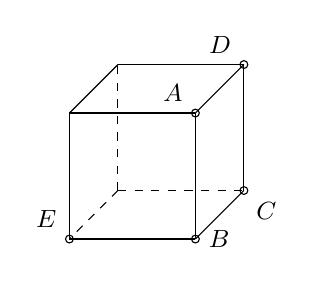
\begin{tikzpicture}
			\begin{scope}[scale=.8] \small
			\draw[dashed] (0,0,0) -- (2,0,0);
			\draw[dashed] (0,0,0) -- (0,2,0);
			\draw[dashed] (0,0,0) -- (0,0,2);
			\draw (2,0,0) -- (2,2,0);
			\draw (2,0,0) -- (2,0,2);
			\draw (0,2,0) -- (0,2,2);
			\draw (0,2,0) -- (2,2,0);
			\draw (0,0,2) -- (0,2,2);
			\draw (0,0,2) -- (2,0,2);
			\draw (2,2,0) -- (2,2,2);
			\draw (2,0,2) -- (2,2,2);
			\draw (0,2,2) -- (2,2,2);
			\tikzstyle{vnode}=[draw, circle, inner sep=1pt];
			\node[vnode] (A) at (2,2,2) [label=150:$A$] {};
			\node[vnode] (B) at (2,0,2) [label=0:$B$] {};
			\node[vnode] (C) at (2,0,0) [label=-40:$C$] {};
			\node[vnode] (D) at (2,2,0) [label=150:$D$] {};
			\node[vnode] (E) at (0,0,2) [label=150:$E$] {};
			\end{scope}
			\end{tikzpicture}

        \end{QBODY}
        \begin{QFROMS}
        \end{QFROMS}
        \begin{QTAGS}\QTAG{B4C1空間向量}\end{QTAGS}
        \begin{QANS}
            $\frac{5}{7}$
        \end{QANS}
        \begin{QSOLLIST}
        \end{QSOLLIST}
        \begin{QEMPTYSPACE}
        \end{QEMPTYSPACE}
    \end{QUESTION}
    \begin{QUESTION}
        \begin{ExamInfo}{100}{學測}{填充}{C}
        \end{ExamInfo}
        \begin{ExamAnsRateInfo}{46}{82}{50}{6}
        \end{ExamAnsRateInfo}
        \begin{QBODY}
			高三甲班共有 20 位男生、15位女生,需推派3位同學參加某項全校性活動。班會中大家決定用抽籤的方式決定參加人選。若每個人中籤的機率相等,則推派的三位同學中有男也有女的機率為 $\TCNBOX{\FR{\TCN\TCN}{\TCN\TCN\TCN}}$ 。
        \end{QBODY}
        \begin{QFROMS}
        \end{QFROMS}
        \begin{QTAGS}\QTAG{B2C3機率}\end{QTAGS}
        \begin{QANS}
            $\frac{90}{119}$
        \end{QANS}
        \begin{QSOLLIST}
        \end{QSOLLIST}
        \begin{QEMPTYSPACE}
        \end{QEMPTYSPACE}
    \end{QUESTION}
    \begin{QUESTION}
        \begin{ExamInfo}{100}{學測}{填充}{D}
        \end{ExamInfo}
        \begin{ExamAnsRateInfo}{32}{73}{21}{2}
        \end{ExamAnsRateInfo}
        \begin{QBODY}
			四邊形 $ABCD$ 中, $AB=1$, $BC=5$, $CD=5$, $DA=7$,且 $\angle DAB= \angle BCD=90^\circ$,則對角線 $\overline{AC}$ 長為 $\TCNBOX{\TCN\TCN}$。
        \end{QBODY}
        \begin{QFROMS}
        \end{QFROMS}
        \begin{QTAGS}\QTAG{B3C1三角}\end{QTAGS}
        \begin{QANS}
            $\sqrt{32}$
        \end{QANS}
        \begin{QSOLLIST}
        \end{QSOLLIST}
        \begin{QEMPTYSPACE}
        \end{QEMPTYSPACE}
    \end{QUESTION}
    \begin{QUESTION}
        \begin{ExamInfo}{100}{學測}{填充}{E}
        \end{ExamInfo}
        \begin{ExamAnsRateInfo}{26}{59}{17}{2}
        \end{ExamAnsRateInfo}
        \begin{QBODY}
			一礦物內含 $A$、$B$、$C$ 三種放射性物質,放射出同一種輻射。已知 $A$、$B$、$C$ 每公克分別會釋放出 1 單位、2 單位、1 單位的輻射強度,又知 $A$ 、 $B$ 、 $C$ 每過半年其質量分別變為原來質量的  $\frac{1}{2}$ 、 $\frac{1}{3}$ 、 $\frac{1}{4}$ 倍。於一年前測得此礦物的輻射強度為 66 單位,而半年前測得此礦物的輻射強度為 22 單位,且目前此礦物的輻射強度為 8 單位,則目前此礦物中 $A$、$B$、$C$ 物質之質量分別為 $\TCNBOX{\TCN}$ 、 $\TCNBOX{\TCN}$ 、 $\TCNBOX{\TCN}$ 公克。
        \end{QBODY}
        \begin{QFROMS}
        \end{QFROMS}
        \begin{QTAGS}\QTAG{B4C3矩陣}\end{QTAGS}
        \begin{QANS}
            $4,1,2$
        \end{QANS}
        \begin{QSOLLIST}
        \end{QSOLLIST}
        \begin{QEMPTYSPACE}
        \end{QEMPTYSPACE}
    \end{QUESTION}
    \begin{QUESTION}
        \begin{ExamInfo}{100}{學測}{填充}{F}
        \end{ExamInfo}
        \begin{ExamAnsRateInfo}{27}{66}{14}{1}
        \end{ExamAnsRateInfo}
        \begin{QBODY}
			設 $E_1:  \frac{x^2}{a^2} +\frac{y^2}{b^2} =1$ (其中 $a>0$ ) 為焦點在 $(3,0)$, $(-3,0)$ 的橢圓;$E_2$ :焦點在 $(3, 0)$ 且準線為 $x = -3$ 的拋物線。 已知 $E_1, E_2$ 的交點在直線 $x=3$ 上,則 $a=\TCNBOX{\TCN+\TCN\sqrt{\TCN}}$。
        \end{QBODY}
        \begin{QFROMS}
        \end{QFROMS}
        \begin{QTAGS}\QTAG{B4C4二次曲線}\end{QTAGS}
        \begin{QANS}
            $3+3\sqrt{2}$
        \end{QANS}
        \begin{QSOLLIST}
        \end{QSOLLIST}
        \begin{QEMPTYSPACE}
        \end{QEMPTYSPACE}
    \end{QUESTION}
    \begin{QUESTION}
        \begin{ExamInfo}{100}{學測}{填充}{G}
        \end{ExamInfo}
        \begin{ExamAnsRateInfo}{31}{74}{17}{2}
        \end{ExamAnsRateInfo}
        \begin{QBODY}
			$H: x-y+z=2$ 為坐標空間中一平面,$L$ 為平面 $H$ 上的一直線。已知點 $P(2,1,1)$ 為 $L$ 上距離原點 $O$ 最近的點,則 $\TCNBOX{(\TCN,\TCN\TCN,\TCN\TCN)}$ 為 $L$ 的方向向量。
        \end{QBODY}
        \begin{QFROMS}
        \end{QFROMS}
        \begin{QTAGS}\QTAG{B4C1空間向量}\end{QTAGS}
        \begin{QANS}
            $(2,-1,-3)$
        \end{QANS}
        \begin{QSOLLIST}
        \end{QSOLLIST}
        \begin{QEMPTYSPACE}
        \end{QEMPTYSPACE}
    \end{QUESTION}
\end{QUESTIONS}

% !TEX encoding = UTF-8 Unicode
% !TEX TS-program = xelatex
\begin{QUESTIONS}
    \begin{QUESTION}
        \begin{ExamInfo}{101}{學測}{單選}{1}
        \end{ExamInfo}
        \begin{ExamAnsRateInfo}{77}{98}{89}{44}
        \end{ExamAnsRateInfo}
        \begin{QBODY}
            $\sqrt{\frac{1}{5^2}+\frac{1}{4^2}+1}$ 等於下列哪一個選項? 
			\begin{QOPS} 
				\QOP 1.01 
				\QOP 1.05 
				\QOP 1.1 
				\QOP 1.15 
				\QOP 1.21
			\end{QOPS}
        \end{QBODY}
        \begin{QFROMS}
        \end{QFROMS}
        \begin{QTAGS}\QTAG{B1C1-1數與數線}\QTAG{B1C1數與式}\end{QTAGS}
        \begin{QANS}
            (2)
        \end{QANS}
        \begin{QSOLLIST}
        \end{QSOLLIST}
        \begin{QEMPTYSPACE}
        \end{QEMPTYSPACE}
    \end{QUESTION}
    \begin{QUESTION}
        \begin{ExamInfo}{101}{學測}{單選}{2}
        \end{ExamInfo}
        \begin{ExamAnsRateInfo}{87}{99}{98}{64}
        \end{ExamAnsRateInfo}
        \begin{QBODY}
            將邊長為 1 公分的正立方體堆疊成一階梯形立體,如下圖所示,其中第 1 層(最下層)有 10 塊,第 2 層有 9 塊,$\cdots$ ,依此類推。當堆疊完 10 層時,該階梯形立體的表面積(即該立體的 前、後、上、下、左、右各表面的面積總和)為多少?
			\begin{QOPS}
				\QOP 75 平方公分 
				\QOP 90 平方公分 
				\QOP 110平方公分 
				\QOP 130平方公分 
				\QOP 150平方公分
			\end{QOPS}
			
			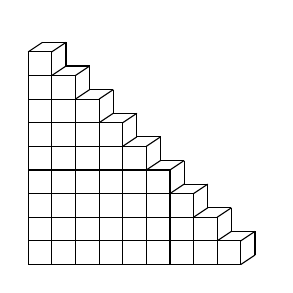
\begin{tikzpicture}[scale=.3]
				\begin{scope}
						\draw (0,0) to (9,0);
						\draw (0,0) to (0,9);
						\foreach \i in {1,2,3,...,9}{
								\draw (0,\i) to (10-\i,\i);
								\draw (\i,0) to (\i,10-\i);
								\draw (\i-1,10-\i) to (\i-.4,10.4-\i);
								\draw (\i,10-\i) to (\i+.6,10.4-\i);
								\draw (\i-.4,10.4-\i) to (\i+.6,10.4-\i);
								\draw (\i+.6,9.4-\i) to (\i+.6,10.4-\i);
						}
						\foreach \i in {10}{
								\draw (0,\i) to (10-\i,\i);
								\draw (\i,0) to (\i,10-\i);
								\draw (\i-1,10-\i) to (\i-.4,10.4-\i);
						}
				\end{scope}
				\end{tikzpicture}
        \end{QBODY}
        \begin{QFROMS}
        \end{QFROMS}
        \begin{QTAGS}\QTAG{B2C1數列級數}\QTAG{B2C1-2級數}\QTAG{等差級數}\end{QTAGS}
        \begin{QANS}
            (5)
        \end{QANS}
        \begin{QSOLLIST}
        \end{QSOLLIST}
        \begin{QEMPTYSPACE}
        \end{QEMPTYSPACE}
    \end{QUESTION}
    \begin{QUESTION}
        \begin{ExamInfo}{101}{學測}{單選}{3}
        \end{ExamInfo}
        \begin{ExamAnsRateInfo}{36}{64}{27}{17}
        \end{ExamAnsRateInfo}
        \begin{QBODY}
            請問 $10^{3.032}$ 最接近下列哪一個選項?(查對數表) 
			\begin{QOPS}
				\QOP 101  
				\QOP 201     
				\QOP 1007 
				\QOP 1076    
				\QOP 2012
			\end{QOPS}
        \end{QBODY}
        \begin{QFROMS}
        \end{QFROMS}
        \begin{QTAGS}\QTAG{B1C3-5指數與對數的應用}\QTAG{B1C3指對數函數}\QTAG{首尾數}\end{QTAGS}
        \begin{QANS}
            (4)
        \end{QANS}
        \begin{QSOLLIST}
        \end{QSOLLIST}
        \begin{QEMPTYSPACE}
        \end{QEMPTYSPACE}
    \end{QUESTION}
    \begin{QUESTION}
        \begin{ExamInfo}{101}{學測}{單選}{4}
        \end{ExamInfo}
        \begin{ExamAnsRateInfo}{45}{77}{43}{15}
        \end{ExamAnsRateInfo}
        \begin{QBODY}
            甲、乙兩校有一樣多的學生參加數學能力測驗,兩校學生測驗成績的分布都很接近常態分布,
			其中甲校學生的平均分數為 60 分,標準差為 10 分;乙校學生的平均分數為 65 分,
			標準差為 5 分。若用粗線表示甲校學生成績分布曲線;細線表示乙校學生成績分布曲線,
			則下列哪一個分布圖較為正確?\\
			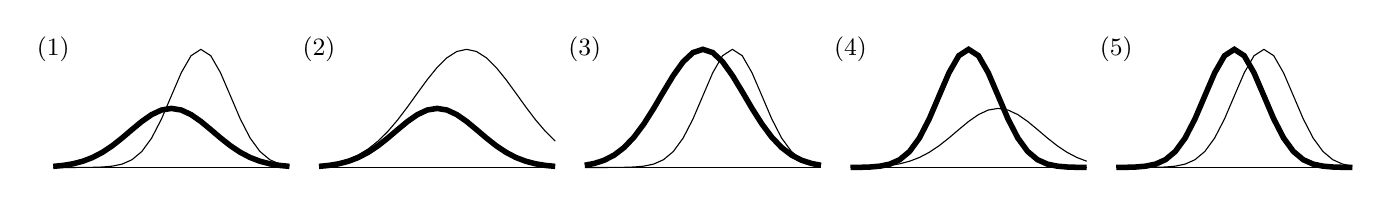
\begin{tikzpicture}[scale=.75]
				\begin{scope}[xshift=0cm,yshift=0cm,domain=-2:2]
				\draw[line width=2pt] plot (\x,{exp(-\x*\x)}) {};
				\draw plot (\x,{2*exp(-(\x-.5)*(\x-.5)/.5)}) {};
				\draw (-2,0) to (2,0);
				\node at (-2,2) {\small (1)};
				\end{scope}
				\begin{scope}[xshift=4.5cm,yshift=0cm,domain=-2:2]
				\draw[line width=2pt] plot (\x,{exp(-\x*\x)}) {};
				\draw plot (\x,{2*exp(-(\x-.5)*(\x-.5)/1.5)}) {};
				\draw (-2,0) to (2,0);
				\node at (-2,2) {\small (2)};
				\end{scope}
				\begin{scope}[xshift=9cm,yshift=0cm,domain=-2:2]
				\draw[line width=2pt] plot (\x,{2*exp(-\x*\x)}) {};
				\draw plot (\x,{2*exp(-(\x-.5)*(\x-.5)/.5)}) {};
				\draw (-2,0) to (2,0);
				\node at (-2,2) {\small (3)};
				\end{scope}
				\begin{scope}[xshift=13.5cm,yshift=0cm,domain=-2:2]
				\draw[line width=2pt] plot (\x,{2*exp(-\x*\x/.5)}) {};
				\draw plot (\x,{1*exp(-(\x-.5)*(\x-.5)/1)}) {};
				\draw (-2,0) to (2,0);
				\node at (-2,2) {\small (4)};
				\end{scope}
				\begin{scope}[xshift=18cm,yshift=0cm,domain=-2:2]
				\draw[line width=2pt] plot (\x,{2*exp(-\x*\x/.5)}) {};
				\draw plot (\x,{2*exp(-(\x-.5)*(\x-.5)/.5)}) {};
				\draw (-2,0) to (2,0);
				\node at (-2,2) {\small (5)};
				\end{scope}
			\end{tikzpicture}
        \end{QBODY}
        \begin{QFROMS}
        \end{QFROMS}
        \begin{QTAGS}\QTAG{B5C1機率與統計}\end{QTAGS}
        \begin{QANS}
            (1)
        \end{QANS}
        \begin{QSOLLIST}
        \end{QSOLLIST}
        \begin{QEMPTYSPACE}
        \end{QEMPTYSPACE}
    \end{QUESTION}
    \begin{QUESTION}
        \begin{ExamInfo}{101}{學測}{單選}{5}
        \end{ExamInfo}
        \begin{ExamAnsRateInfo}{51}{91}{46}{16}
        \end{ExamAnsRateInfo}
        \begin{QBODY}
            若正實數 $x, y$ 滿足 $\log_{10} x =2.8  $, $\log_{10} y = 5.6$,則 $\log_{10} ( x^2 + y)$ 最接近下列哪一個選項的值?
			\begin{QOPS} 
				\QOP   2.8    
				\QOP   5.6 
				\QOP   5.9 
				\QOP   8.4 
				\QOP   11.2 。
			\end{QOPS}
        \end{QBODY}
        \begin{QFROMS}
        \end{QFROMS}
        \begin{QTAGS}\QTAG{B1C3-3對數}\QTAG{B1C3指對數函數}\QTAG{對數律}\end{QTAGS}
        \begin{QANS}
            (3)
        \end{QANS}
        \begin{QSOLLIST}
        \end{QSOLLIST}
        \begin{QEMPTYSPACE}
        \end{QEMPTYSPACE}
    \end{QUESTION}
    \begin{QUESTION}
        \begin{ExamInfo}{101}{學測}{單選}{6}
        \end{ExamInfo}
        \begin{ExamAnsRateInfo}{66}{84}{71}{43}
        \end{ExamAnsRateInfo}
        \begin{QBODY}
            箱中有編號分別為 $0,1, 2, \cdots ,9$   的十顆球。隨機抽取一球,將球放回後,再隨機抽取一球。請問這兩球編號相減的絕對值為下列哪一個選項時,其出現的機率最大?
			\begin{QOPS}
				\QOP  0  
				\QOP  1 
				\QOP  4 
				\QOP  5 
				\QOP  9
			\end{QOPS}
        \end{QBODY}
        \begin{QFROMS}
        \end{QFROMS}
        \begin{QTAGS}\QTAG{B2C3機率}\QTAG{B2C3-2機率的定義與性質}\end{QTAGS}
        \begin{QANS}
            (2)
        \end{QANS}
        \begin{QSOLLIST}
        \end{QSOLLIST}
        \begin{QEMPTYSPACE}
        \end{QEMPTYSPACE}
    \end{QUESTION}
    \begin{QUESTION}
        \begin{ExamInfo}{101}{學測}{單選}{7}
        \end{ExamInfo}
        \begin{ExamAnsRateInfo}{37}{45}{34}{32}
        \end{ExamAnsRateInfo}
        \begin{QBODY}
            空間坐標中有一球面(半徑大於0)與平面 $3x+4y=0$ 相切於原點,請問此球面與三個坐標軸一共有多少個交點? 
			\begin{QOPS} 
				\QOP $1$ 
				\QOP $2$ 
				\QOP $3$ 
				\QOP $4$ 
				\QOP $5$
			\end{QOPS}
        \end{QBODY}
        \begin{QFROMS}
        \end{QFROMS}
        \begin{QTAGS}\QTAG{不是99課綱}\end{QTAGS}
        \begin{QANS}
            (3)
        \end{QANS}
        \begin{QSOLLIST}
        \end{QSOLLIST}
        \begin{QEMPTYSPACE}
        \end{QEMPTYSPACE}
    \end{QUESTION}
\end{QUESTIONS}
\begin{QUESTIONS}
    \begin{QUESTION}
        \begin{ExamInfo}{101}{學測}{多選}{8}
        \end{ExamInfo}
        \begin{ExamAnsRateInfo}{56}{92}{58}{18}
        \end{ExamAnsRateInfo}
        \begin{QBODY}
            設 $f(x) = x^4-5x^3+x^2+ax+b$ 為實係數多項式,且知 $f( i)  =0 $。請問下列哪些選項是多項式方程式 $f (x ) = 0$ 的根?
		\begin{QOPS} 
			\QOP  $-i$ 
			\QOP  $0$
			\QOP  $1$ 
			\QOP  $-5$ 
			\QOP  $5$
		\end{QOPS}
        \end{QBODY}
        \begin{QFROMS}
        \end{QFROMS}
        \begin{QTAGS}\QTAG{B1C2多項式函數}\QTAG{B1C2-3多項式方程式}\QTAG{虛根定理}\end{QTAGS}
        \begin{QANS}
            (1)(2)(5)
        \end{QANS}
        \begin{QSOLLIST}
        \end{QSOLLIST}
        \begin{QEMPTYSPACE}
        \end{QEMPTYSPACE}
    \end{QUESTION}
    \begin{QUESTION}
        \begin{ExamInfo}{101}{學測}{多選}{9}
        \end{ExamInfo}
        \begin{ExamAnsRateInfo}{51}{77}{51}{25}
        \end{ExamAnsRateInfo}
        \begin{QBODY}
            三角形 ABC 是一個邊長為 3 的正三角形,如下圖所示。若在每一邊的兩個三等分點中,各選取一點連成三角形,則下列哪些選項是正確的?

			\begin{QOPS} 
				\QOP 依此方法可能連成的三角形一共有 8 個
				\QOP 這些可能連成的三角形中,恰有 2 個是銳角三角形 \QOP 這些可能連成的三角形中,恰有 3 個是直角三角形
				\QOP 這些可能連成的三角形中,恰有 3 個是鈍角三角形
				\QOP 這些可能連成的三角形中,恰有 1 個是正三角形
			\end{QOPS}
        \end{QBODY}
        \begin{QFROMS}
        \end{QFROMS}
        \begin{QTAGS}\QTAG{乘法原理加法原理}\QTAG{B2C2-1簡單的邏輯與集合}\QTAG{B2C2排列組合}\end{QTAGS}
        \begin{QANS}
            (1)(2)
        \end{QANS}
        \begin{QSOLLIST}
        \end{QSOLLIST}
        \begin{QEMPTYSPACE}
        \end{QEMPTYSPACE}
    \end{QUESTION}
    \begin{QUESTION}
        \begin{ExamInfo}{101}{學測}{多選}{10}
        \end{ExamInfo}
        \begin{ExamAnsRateInfo}{36}{66}{27}{15}
        \end{ExamAnsRateInfo}
        \begin{QBODY}
            設 $O$ 為複數平面上的原點,並令點 $A,B$ 分別代表非零複數 $z,w$。若 $\angle AOB = 90^\circ$,則下列哪些選項必為負實數?
		\begin{QOPS} 
			\QOP $\frac{z}{w}$    
			\QOP $zw$    
			\QOP $(zw)^2$ 
			\QOP $\frac{z^2}{w^2}$ 
			\QOP $(z\overline{w})^2$ (其中 $\overline{w}$ 為 $w$ 的共軛複數)
		\end{QOPS}
        \end{QBODY}
        \begin{QFROMS}
        \end{QFROMS}
        \begin{QTAGS}\QTAG{B5C2三角函數II}\end{QTAGS}
        \begin{QANS}
            (4)(5)
        \end{QANS}
        \begin{QSOLLIST}
        \end{QSOLLIST}
        \begin{QEMPTYSPACE}
        \end{QEMPTYSPACE}
    \end{QUESTION}
    \begin{QUESTION}
        \begin{ExamInfo}{101}{學測}{多選}{11}
        \end{ExamInfo}
        \begin{ExamAnsRateInfo}{37}{62}{29}{20}
        \end{ExamAnsRateInfo}
        \begin{QBODY}
            若實數 $a, b, c,  d$ 使得聯立方程組
			$\left\{\begin{array}{ccc} ax+8y & = & c \\ x-4y & = & 3 \end{array}\right.$
			有解,且聯立方程組 $\left\{\begin{array}{ccc} -3x+by & = & d \\ x-4y & = & 3 \end{array}\right.$
			無解,則下列哪些選項一定正確? 
			\begin{QOPS} 
				\QOP  $a \neq -2$
				\QOP  $c = -6$    
				\QOP  $b =12$    
				\QOP  $d \neq -9$ 
				\QOP  聯立方程組 $\left\{\begin{array}{ccc} ax+8y & = & c \\ -3x+by & = & d \end{array}\right.$無解
			\end{QOPS}
        \end{QBODY}
        \begin{QFROMS}
        \end{QFROMS}
        \begin{QTAGS}\QTAG{B3C3平面向量}\QTAG{B3C3-3面積與二階行列式}\end{QTAGS}
        \begin{QANS}
            (3)(4)
        \end{QANS}
        \begin{QSOLLIST}
        \end{QSOLLIST}
        \begin{QEMPTYSPACE}
        \end{QEMPTYSPACE}
    \end{QUESTION}
    \begin{QUESTION}
        \begin{ExamInfo}{101}{學測}{多選}{12}
        \end{ExamInfo}
        \begin{ExamAnsRateInfo}{42}{64}{40}{22}
        \end{ExamAnsRateInfo}
        \begin{QBODY}
            在坐標平面上,廣義角 $\theta$ 的頂點為原點 $O$,始邊為 $x$ 軸的正向,且滿足 $\tan \theta =\frac{2}{3}$。若 $\theta$ 的終邊上有一點 $P$ ,其 $y$ 坐標為 $-4$ ,則下列哪些選項一定正確? 
			\begin{QOPS} 
				\QOP $P$ 的 $x$ 坐標為 6 
				\QOP $\overline{OP} = 2\sqrt{13}$ 
				\QOP $\cos\theta = \frac{3}{\sqrt{13}}$ 
				\QOP $\sin 2\theta >0$ 
				\QOP $\cos \frac{\theta}{2} <0$。
			\end{QOPS}
        \end{QBODY}
        \begin{QFROMS}
        \end{QFROMS}
        \begin{QTAGS}\QTAG{廣義角}\QTAG{B3C1三角}\QTAG{B3C1-2廣義角與極坐標}\end{QTAGS}
        \begin{QANS}
            (2)(4)
        \end{QANS}
        \begin{QSOLLIST}
        \end{QSOLLIST}
        \begin{QEMPTYSPACE}
        \end{QEMPTYSPACE}
    \end{QUESTION}
    \begin{QUESTION}
        \begin{ExamInfo}{101}{學測}{多選}{13}
        \end{ExamInfo}
        \begin{ExamAnsRateInfo}{45}{79}{40}{16}
        \end{ExamAnsRateInfo}
        \begin{QBODY}
            平面上兩點 $F_1,F_2$ 滿足 $F_1F_2 =4$。設 $d$ 為一實數,令 $\Gamma$ 表示平面上滿足 $|PF_1 -PF_2|=d$ 的所有 $P$ 點所成的圖形,又令 $C$ 為平面上以 $F_1$ 為圓心、 6 為半徑的圓。請問下列哪些選項是正確的?
			\begin{QOPS}
				\QOP 當 $d = 0$ 時,$\Gamma$ 為直線 
				\QOP 當 $d =1$ 時, $\Gamma$ 為雙曲線 
				\QOP 當 $\Gamma = 2$ 時, $\Gamma$ 與圓 $C$ 交於兩點 
				\QOP 當 $d = 4$ 時, $\Gamma$ 與圓 $C$ 交於四點 
				\QOP 當 $d = 8$ 時, $\Gamma$ 不存在。
			\end{QOPS}
        \end{QBODY}
        \begin{QFROMS}
        \end{QFROMS}
        \begin{QTAGS}\QTAG{B4C4-3雙曲線}\QTAG{B4C4二次曲線}\QTAG{圖形}\end{QTAGS}
        \begin{QANS}
            (1)(2)(5)
        \end{QANS}
        \begin{QSOLLIST}
        \end{QSOLLIST}
        \begin{QEMPTYSPACE}
        \end{QEMPTYSPACE}
    \end{QUESTION}
\end{QUESTIONS}
\begin{QUESTIONS}
    \begin{QUESTION}
        \begin{ExamInfo}{101}{學測}{填充}{A}
        \end{ExamInfo}
        \begin{ExamAnsRateInfo}{44}{86}{39}{7}
        \end{ExamAnsRateInfo}
        \begin{QBODY}
            若首項為 $a$,公比為 $0.01$ 的無窮等比級數和等於循環小數 $1.\overline{2}$,則 $a=\TCNBOX{\TCN.\TCN\TCN}$ 。
        \end{QBODY}
        \begin{QFROMS}
        \end{QFROMS}
        \begin{QTAGS}\QTAG{B6C1函數與極限}\end{QTAGS}
        \begin{QANS}
            $1.21$
        \end{QANS}
        \begin{QSOLLIST}
        \end{QSOLLIST}
        \begin{QEMPTYSPACE}
        \end{QEMPTYSPACE}
    \end{QUESTION}
    \begin{QUESTION}
        \begin{ExamInfo}{101}{學測}{填充}{B}
        \end{ExamInfo}
        \begin{ExamAnsRateInfo}{39}{71}{39}{7}
        \end{ExamAnsRateInfo}
        \begin{QBODY}
            設 $A(1,1)$, $B(3,5)$, $C(5,3)$, $D(0,-7)$, $E(2,-3)$ 及 $F(8,-6)$ 為坐標平面上的六個點。若直線 $L$ 分別與三角形 $ABC$ 及三角形 $DEF$ 各恰有一個交點,則 $L$ 的斜率之最小可能值為 $\TCNBOX{\TCN\TCN}$。
        \end{QBODY}
        \begin{QFROMS}
        \end{QFROMS}
        \begin{QTAGS}\QTAG{B3C2-1直線方程式及其圖形}\QTAG{B3C2直線與圓}\end{QTAGS}
        \begin{QANS}
            $-3$
        \end{QANS}
        \begin{QSOLLIST}
        \end{QSOLLIST}
        \begin{QEMPTYSPACE}
        \end{QEMPTYSPACE}
    \end{QUESTION}
    \begin{QUESTION}
        \begin{ExamInfo}{101}{學測}{填充}{C}
        \end{ExamInfo}
        \begin{ExamAnsRateInfo}{56}{90}{65}{13}
        \end{ExamAnsRateInfo}
        \begin{QBODY}
            小明在天文網站上看到以下的資訊「可利用北斗七星斗杓的天璇與天樞這兩顆星來尋找北極星:由天璇起始向天樞的方向延伸便可找到北極星,其中天樞與北極星的距離為天樞與天璇距離的 5 倍。」今小明將所見的星空想像成一個坐標平面,其中天璇的坐標為 (9,8) 及天樞的坐標為 (7,11),依上述資訊可以推得北極星的坐標為 $\TCNBOX{(\TCN\TCN,\TCN\TCN)}$。
        \end{QBODY}
        \begin{QFROMS}
        \end{QFROMS}
        \begin{QTAGS}\QTAG{線性組合}\QTAG{B3C3-1平面向量的表示法}\QTAG{B3C3平面向量}\end{QTAGS}
        \begin{QANS}
            $(-3,26)$
        \end{QANS}
        \begin{QSOLLIST}
        \end{QSOLLIST}
        \begin{QEMPTYSPACE}
        \end{QEMPTYSPACE}
    \end{QUESTION}
    \begin{QUESTION}
        \begin{ExamInfo}{101}{學測}{填充}{D}
        \end{ExamInfo}
        \begin{ExamAnsRateInfo}{37}{83}{27}{1}
        \end{ExamAnsRateInfo}
        \begin{QBODY}
            設點 $A(-2,2)$、$B(4,8)$ 為坐標平面上兩點,且點 $C$ 在二次函數 $y = \frac{1}{2}x^2$ 的圖形上變動。當 $C$ 點的 $x$ 坐標為 $\TCNBOX{\TCN\TCN}$ 時,內積 $\lvec{AB}\cdot \lvec{AC}$ 有最小值 $\TCNBOX{\TCN\TCN}$ 。
        \end{QBODY}
        \begin{QFROMS}
        \end{QFROMS}
        \begin{QTAGS}\QTAG{B3C3-2平面向量的內積}\QTAG{B3C3平面向量}\end{QTAGS}
        \begin{QANS}
            $-1,-3$
        \end{QANS}
        \begin{QSOLLIST}
        \end{QSOLLIST}
        \begin{QEMPTYSPACE}
        \end{QEMPTYSPACE}
    \end{QUESTION}
    \begin{QUESTION}
        \begin{ExamInfo}{101}{學測}{填充}{E}
        \end{ExamInfo}
        \begin{ExamAnsRateInfo}{46}{85}{39}{14}
        \end{ExamAnsRateInfo}
        \begin{QBODY}
            在邊長為13的正三角形 $ABC$ 上各邊分別取一點 $P,Q,R$,使得 $APQR$ 形成一平行四邊形,如右圖所示:若平行四邊形 $APQR$ 的面積為 $20\sqrt{3}$,則線段 PR 的長度為 $\TCNBOX{\TCN}$ 。
			
			\begin{tikzpicture}[scale=.15]
				\begin{scope}\small
						\foreach \n/\i/\j/\l in{B/0/0/240,C/0/13/300,Q/0/8/300,A/60/13/90,P/60/8/120}{
								\node[inner sep=0pt,draw,circle] (v\n)at (\i:\j) [label=\l:$\n$] {};
						}
						\node[inner sep=0pt,draw,circle]  (vR) at ($(0:13)!.38!(60:13)$) [label=30:$R$] {};
						\foreach \i/\j in{B/C,C/A,A/B,P/Q,Q/R}
								\draw (v\i) to (v\j);
						\draw[dotted] (vP) to (vR);
				\end{scope}
			\end{tikzpicture}
        \end{QBODY}
        \begin{QFROMS}
        \end{QFROMS}
        \begin{QTAGS}\QTAG{面積}\QTAG{B3C1-3正弦定理與餘弦定理}\QTAG{B3C1三角}\end{QTAGS}
        \begin{QANS}
            $7$
        \end{QANS}
        \begin{QSOLLIST}
        \end{QSOLLIST}
        \begin{QEMPTYSPACE}
        \end{QEMPTYSPACE}
    \end{QUESTION}
    \begin{QUESTION}
        \begin{ExamInfo}{101}{學測}{填充}{F}
        \end{ExamInfo}
        \begin{ExamAnsRateInfo}{40}{80}{37}{3}
        \end{ExamAnsRateInfo}
        \begin{QBODY}
            設 $m,n$ 為正實數,橢圓 $\frac{x^2}{m}  + \frac{y^2}{n} =1$ 的焦點分別為 $F_1 (0,2)$ 與 $F_2 (0,-2)$。若此橢圓上有一點 $P$ 使得 $\triangle PF_1 F_2$ 為一正三角形,則 $m=\TCNBOX{\TCN\TCN} , n = \TCNBOX{\TCN\TCN}$。
        \end{QBODY}
        \begin{QFROMS}
        \end{QFROMS}
        \begin{QTAGS}\QTAG{B4C4二次曲線}\QTAG{B4C4-2橢圓}\end{QTAGS}
        \begin{QANS}
            $12, 16$
        \end{QANS}
        \begin{QSOLLIST}
        \end{QSOLLIST}
        \begin{QEMPTYSPACE}
        \end{QEMPTYSPACE}
    \end{QUESTION}
    \begin{QUESTION}
        \begin{ExamInfo}{101}{學測}{填充}{G}
        \end{ExamInfo}
        \begin{ExamAnsRateInfo}{23}{54}{13}{2}
        \end{ExamAnsRateInfo}
        \begin{QBODY}
            坐標空間中,在六個平面 $x=\frac{14}{13}$,  $x=\frac{1}{13}$ , $y=1$,  $y=-1$, $z=-1$ 及 $z=-4$ 所圍成的長方體上隨機選取兩個相異頂點。若每個頂點被選取的機率相同,則選到兩個頂點的距離大於 3 之機率為 $\TCNBOX{\FR{\TCN}{\TCN}}$ 。
        \end{QBODY}
        \begin{QFROMS}
        \end{QFROMS}
        \begin{QTAGS}\QTAG{B4C2空間中的平面與直線}\QTAG{B4C2-1平面方程式}\QTAG{B2C3機率}\QTAG{B2C3-2機率的定義與性質}\QTAG{距離}\end{QTAGS}
        \begin{QANS}
            $\FR{3}{7}$
        \end{QANS}
        \begin{QSOLLIST}
        \end{QSOLLIST}
        \begin{QEMPTYSPACE}
        \end{QEMPTYSPACE}
    \end{QUESTION}
\end{QUESTIONS}

    \begin{QUESTION}
        \begin{ExamInfo}{102}{學測}{單選}{1}
        \end{ExamInfo}
        \begin{ExamAnsRateInfo}{70}{88}{73}{49}
        \end{ExamAnsRateInfo}
        \begin{QBODY}
            學校規定上學期成績需同時滿足以下兩項要求,才有資格參選模範生。\\
				一、國文成績或英文成績70分(含)以上;\\
				二、數學成績及格。\\
				已知小文上學期國文65分而且他不符合參選模範生資格。請問下列哪一個選項的推論是正確的?
				\begin{QOPS}
					\QOP 小文的英文成績未達70分
					\QOP 小文的數學成績不及格
					\QOP 小文的英文成績70分以上但數學成績不及格
					\QOP 小文的英文成績未達70分且數學成績不及格
					\QOP 小文的英文成績未達70分或數學成績不及格
				\end{QOPS}
        \end{QBODY}
        \begin{QFROMS}
        \end{QFROMS}
        \begin{QTAGS}\QTAG{邏輯}\QTAG{B2C2-1簡單的邏輯與集合}\QTAG{B2C2排列組合}\end{QTAGS}
        \begin{QANS}
            (5)
        \end{QANS}
        \begin{QSOLLIST}
        \end{QSOLLIST}
        \begin{QEMPTYSPACE}
        \end{QEMPTYSPACE}
    \end{QUESTION}
    \begin{QUESTION}
        \begin{ExamInfo}{102}{學測}{單選}{2}
        \end{ExamInfo}
        \begin{ExamAnsRateInfo}{66}{90}{72}{36}
        \end{ExamAnsRateInfo}
        \begin{QBODY}
            令$a={{2.6}^{10}}-{{2.6}^{9}}$,$b={{2.6}^{11}}-{{2.6}^{10}}$,$c=\FR{{{2.6}^{11}}-{{2.6}^{9}}}{2}$。請選出正確的大小關係。
			\begin{QOPS}
				\QOP $a>b>c$
				\QOP $a>c>b$
				\QOP $b>a>c$
				\QOP $b>c>a$
				\QOP $c>b>a$
			\end{QOPS}
        \end{QBODY}
        \begin{QFROMS}
        \end{QFROMS}
        \begin{QTAGS}\QTAG{圖形}\QTAG{B1C3-2指數函數}\QTAG{B1C3指對數函數}\end{QTAGS}
        \begin{QANS}
            (4)
        \end{QANS}
        \begin{QSOLLIST}
        \end{QSOLLIST}
        \begin{QEMPTYSPACE}
        \end{QEMPTYSPACE}
    \end{QUESTION}
    \begin{QUESTION}
        \begin{ExamInfo}{102}{學測}{單選}{3}
        \end{ExamInfo}
        \begin{ExamAnsRateInfo}{35}{67}{26}{12}
        \end{ExamAnsRateInfo}
        \begin{QBODY}
            袋子裡有3顆白球,$\,2\,$顆黑球。由甲、乙、丙三人依序各抽取1顆球,抽取後不放回。若每顆球被取出的機會相等,請問在甲和乙抽到相同顏色球的條件下,丙抽到白球之條件機率為何?
			\begin{QOPS}
				\QOP $\FR{1}{3}$	
				\QOP $\FR{5}{12}$	
				\QOP $\FR{1}{2}$
				\QOP $\FR{3}{5}$	
				\QOP $\FR{2}{3}$
			\end{QOPS}
        \end{QBODY}
        \begin{QFROMS}
        \end{QFROMS}
        \begin{QTAGS}\QTAG{B2C3機率}\QTAG{B2C3-3條件機率與貝氏定理}\end{QTAGS}
        \begin{QANS}
            (3)
        \end{QANS}
        \begin{QSOLLIST}
        \end{QSOLLIST}
        \begin{QEMPTYSPACE}
        \end{QEMPTYSPACE}
    \end{QUESTION}
    \begin{QUESTION}
        \begin{ExamInfo}{102}{學測}{單選}{4}
        \end{ExamInfo}
        \begin{ExamAnsRateInfo}{30}{46}{25}{19}
        \end{ExamAnsRateInfo}
        \begin{QBODY}
            已知以下各選項資料的迴歸直線(最適合直線)皆相同且皆為負相關,請選出相關係數最小的選項。
			\begin{QOPS}
				\QOP $\begin{matrix}
				   x & 2 & 3 & 5  \\
				   y & 1 & 13 & 1  \\
				\end{matrix}$	
				\QOP $\begin{matrix}
				   x & 2 & 3 & 5  \\
				   y & 3 & 10 & 2  \\
				\end{matrix}$ 	
				\QOP $\begin{matrix}
				   x & 2 & 3 & 5  \\
				   y & 5 & 7 & 3  \\
				\end{matrix}$ 
				\QOP $\begin{matrix}
				   x & 2 & 3 & 5  \\
				   y & 9 & 1 & 5  \\
				\end{matrix}$	
				\QOP $\begin{matrix}
				   x & 2 & 3 & 5  \\
				   y & 7 & 4 & 4  \\
				\end{matrix}$
			\end{QOPS}
        \end{QBODY}
        \begin{QFROMS}
        \end{QFROMS}
        \begin{QTAGS}\QTAG{B2C4-2二維數據分析}\QTAG{B2C4數據分析}\QTAG{相關係數}\QTAG{迴歸直線}\end{QTAGS}
        \begin{QANS}
            (5)
        \end{QANS}
        \begin{QSOLLIST}
        \end{QSOLLIST}
        \begin{QEMPTYSPACE}
        \end{QEMPTYSPACE}
    \end{QUESTION}
    \begin{QUESTION}
        \begin{ExamInfo}{102}{學測}{單選}{5}
        \end{ExamInfo}
        \begin{ExamAnsRateInfo}{50}{75}{50}{25}
        \end{ExamAnsRateInfo}
        \begin{QBODY}
            將24顆雞蛋分裝到紅、黃、綠的三個籃子。每個籃子都要有雞蛋,且黃、綠兩
			個籃子裡都裝奇數顆。請選出分裝的方法數。
			\begin{QOPS}
					\QOP $55  $
					\QOP $66  $
					\QOP $132 $
					\QOP $198 $
					\QOP $253 $
			\end{QOPS}
        \end{QBODY}
        \begin{QFROMS}
        \end{QFROMS}
        \begin{QTAGS}\QTAG{重複組合}\QTAG{B2C2排列組合}\QTAG{B2C2-3組合}\end{QTAGS}
        \begin{QANS}
            (2)
        \end{QANS}
        \begin{QSOLLIST}
        \end{QSOLLIST}
        \begin{QEMPTYSPACE}
        \end{QEMPTYSPACE}
    \end{QUESTION}
    \begin{QUESTION}
        \begin{ExamInfo}{102}{學測}{單選}{6}
        \end{ExamInfo}
        \begin{ExamAnsRateInfo}{39}{71}{31}{15}
        \end{ExamAnsRateInfo}
        \begin{QBODY}
            莎韻觀測遠方等速率垂直上升的熱氣球。在上午$10:00$熱氣球的仰角為$30{}^\circ $,到上午$10:10$仰角變成$34{}^\circ $。請利用下表判斷到上午$10:30$時,熱氣球的仰角最接近下列哪一個度數?
			\begin{tabular}{|c|c|c|c|c|c|c|c|}
			\hline
			$\theta $		& $30{}^\circ $ & $34{}^\circ $ & 	$39{}^\circ $	&  $40{}^\circ $   & $41{}^\circ $ & $42{}^\circ $	& $43{}^\circ $  \\\hline
			$\sin \theta $	& 0.500	        &    0.559	    &       0.629	    &     0.643	       &   0.656	   &       0.669	&      0.682     \\\hline
			$\cos \theta $	& 0.866	        &    0.829	    &       0.777	    &     0.766	       &   0.755	   &       0.743	&      0.731     \\\hline
			$\tan \theta $	& 0.577	        &    0.675	    &       0.810	    &     0.839	       &   0.869	   &       0.900	&      0.933     \\\hline
			\end{tabular}
			\begin{QOPS}
				\QOP $39{}^\circ $
				\QOP $40{}^\circ $
				\QOP $41{}^\circ $
				\QOP $42{}^\circ $
				\QOP $43{}^\circ $
			\end{QOPS}
        \end{QBODY}
        \begin{QFROMS}
        \end{QFROMS}
        \begin{QTAGS}\QTAG{B3C1-5三角測量}\QTAG{B3C1三角}\end{QTAGS}
        \begin{QANS}
            (3)
        \end{QANS}
        \begin{QSOLLIST}
        \end{QSOLLIST}
        \begin{QEMPTYSPACE}
        \end{QEMPTYSPACE}
    \end{QUESTION}
    \begin{QUESTION}
        \begin{ExamInfo}{102}{學測}{多選}{7}
        \end{ExamInfo}
        \begin{ExamAnsRateInfo}{60}{85}{67}{28}
        \end{ExamAnsRateInfo}
        \begin{QBODY}
            設$n$為正整數,符號${{\left[ \begin{matrix}
			   1 & 1  \\
			   0 & 2  \\
			\end{matrix} \right]}^{n}}$代表矩陣$\left[ \begin{matrix}
			   1 & 1  \\
			   0 & 2  \\
			\end{matrix} \right]$自乘$n$次。令${{\left[ \begin{matrix}
			   1 & 1  \\
			   0 & 2  \\
			\end{matrix} \right]}^{n}}=\left[ \begin{matrix}
			   {{a}_{n}} & {{b}_{n}}  \\
			   {{c}_{n}} & {{d}_{n}}  \\
			\end{matrix} \right]$,請選出正確的選項。
			\begin{QOPS}
				\QOP ${{a}_{2}}=1$
				\QOP ${{a}_{1}},{{a}_{2}},{{a}_{3}}$為等比數列
				\QOP ${{d}_{1}},{{d}_{2}},{{d}_{3}}$為等比數列
				\QOP ${{b}_{1}},{{b}_{2}},{{b}_{3}}$為等差數列
				\QOP ${{c}_{1}},{{c}_{2}},{{c}_{3}}$為等差數列
			\end{QOPS}
        \end{QBODY}
        \begin{QFROMS}
        \end{QFROMS}
        \begin{QTAGS}\QTAG{矩陣乘法}\QTAG{B4C3矩陣}\QTAG{等差數列}\QTAG{B2C1數列級數}\QTAG{等比數列}\QTAG{B2C1-1數列}\QTAG{B4C3-2矩陣的運算}\end{QTAGS}
        \begin{QANS}
            (1)(2)(3)(5)
        \end{QANS}
        \begin{QSOLLIST}
        \end{QSOLLIST}
        \begin{QEMPTYSPACE}
        \end{QEMPTYSPACE}
    \end{QUESTION}
    \begin{QUESTION}
        \begin{ExamInfo}{102}{學測}{多選}{8}
        \end{ExamInfo}
        \begin{ExamAnsRateInfo}{47}{68}{50}{23}
        \end{ExamAnsRateInfo}
        \begin{QBODY}
            設$a>1>b>0$,關於下列不等式,請選出正確的選項。
			\begin{QOPS}
				\QOP ${{(-a)}^{7}}>{{(-a)}^{9}}$
				\QOP ${{b}^{-9}}>{{b}^{-7}}$
				\QOP ${{\log }_{10}}\FR{1}{a}>{{\log }_{10}}\FR{1}{b}$
				\QOP ${{\log }_{a}}1>{{\log }_{b}}1$
				\QOP ${{\log }_{a}}b\ge {{\log }_{b}}a$
			\end{QOPS}
        \end{QBODY}
        \begin{QFROMS}
        \end{QFROMS}
        \begin{QTAGS}\QTAG{B1C3-4對數函數}\QTAG{B1C3指對數函數}\QTAG{不等式}\end{QTAGS}
        \begin{QANS}
            (1)(2)
        \end{QANS}
        \begin{QSOLLIST}
        \end{QSOLLIST}
        \begin{QEMPTYSPACE}
        \end{QEMPTYSPACE}
    \end{QUESTION}
    \begin{QUESTION}
        \begin{ExamInfo}{102}{學測}{多選}{9}
        \end{ExamInfo}
        \begin{ExamAnsRateInfo}{43}{64}{40}{25}
        \end{ExamAnsRateInfo}
        \begin{QBODY}
            設$a<b<c$。已知實係數多項式函數$y=f(x)$的圖形為一開口向上的拋物線,且與$x$軸交於$(a,0)$、$(b,0)$兩點;實係數多項式函數$y=g(x)$的圖形亦為一開口向上的拋物線,且跟$x$軸相交於$(b,0)$、$(c,0)$兩點。請選出$y=f(x)+g(x)$的圖形可能的選項。
			\begin{QOPS}
				\QOP 水平直線
				\QOP 和$x$軸僅交於一點的直線
				\QOP 和$x$軸無交點的拋物線
				\QOP 和$x$軸僅交於一點的拋物線
				\QOP 和$x$軸交於兩點的拋物線
			\end{QOPS}
        \end{QBODY}
        \begin{QFROMS}
        \end{QFROMS}
        \begin{QTAGS}\QTAG{B1C2多項式函數}\QTAG{圖形}\QTAG{二次多項式}\QTAG{B1C2-1簡單的多項式及圖形}\end{QTAGS}
        \begin{QANS}
            (4)(5)
        \end{QANS}
        \begin{QSOLLIST}
        \end{QSOLLIST}
        \begin{QEMPTYSPACE}
        \end{QEMPTYSPACE}
    \end{QUESTION}
    \begin{QUESTION}
        \begin{ExamInfo}{102}{學測}{多選}{10}
        \end{ExamInfo}
        \begin{ExamAnsRateInfo}{36}{60}{30}{18}
        \end{ExamAnsRateInfo}
        \begin{QBODY}
            坐標平面上考慮兩點${{Q}_{1}}(1,0),{{Q}_{2}}(-1,0)$。在下列各方程式的圖形中,請選出其上至少有一點$P$滿足內積 $\lvec{PQ_{1}}\cdot \lvec{PQ_{2}}<0$的選項。
		\begin{QOPS}
			\QOP $y=\FR{1}{2}$  
			\QOP $y={{x}^{2}}+1$ 
			\QOP $-{{x}^{2}}+2{{y}^{2}}=1$
			\QOP $4{{x}^{2}}+{{y}^{2}}=1$
			\QOP $\FR{{{x}^{2}}}{2}-\FR{{{y}^{2}}}{2}=1$
		\end{QOPS}
        \end{QBODY}
        \begin{QFROMS}
        \end{QFROMS}
        \begin{QTAGS}\QTAG{B3C3-2平面向量的內積}\QTAG{B3C3平面向量}\QTAG{夾角}\QTAG{圖形}\end{QTAGS}
        \begin{QANS}
            (1)(3)(4)
        \end{QANS}
        \begin{QSOLLIST}
        \end{QSOLLIST}
        \begin{QEMPTYSPACE}
        \end{QEMPTYSPACE}
    \end{QUESTION}
    \begin{QUESTION}
        \begin{ExamInfo}{102}{學測}{多選}{11}
        \end{ExamInfo}
        \begin{ExamAnsRateInfo}{42}{58}{45}{23}
        \end{ExamAnsRateInfo}
        \begin{QBODY}
            設${{F}_{1}},{{F}_{2}}$為橢圓$\Gamma $的兩個焦點。$S$為以${{F}_{1}}$為中心的正方形($S$的各邊可不與$\Gamma $的對稱軸平行)。試問$S$可能有幾個頂點落在$\Gamma $上?
			\begin{QOPS}
				\QOP 1
				\QOP 2
				\QOP 3
				\QOP 4
				\QOP 0
			\end{QOPS}
        \end{QBODY}
        \begin{QFROMS}
        \end{QFROMS}
        \begin{QTAGS}\QTAG{B4C4二次曲線}\QTAG{B4C4-2橢圓}\end{QTAGS}
        \begin{QANS}
            (1)(2)(5)
        \end{QANS}
        \begin{QSOLLIST}
        \end{QSOLLIST}
        \begin{QEMPTYSPACE}
        \end{QEMPTYSPACE}
    \end{QUESTION}
    \begin{QUESTION}
        \begin{ExamInfo}{102}{學測}{多選}{12}
        \end{ExamInfo}
        \begin{ExamAnsRateInfo}{45}{67}{46}{22}
        \end{ExamAnsRateInfo}
        \begin{QBODY}
            設實數組成的數列$\left\langle {{a}_{n}} \right\rangle $是公比為$-\,0.8$的等比數列,實數組成的數列$\left\langle {{b}_{n}} \right\rangle $是首項為10的等差數列。已知${{a}_{9}}>{{b}_{9}}$且${{a}_{10}}>{{b}_{10}}$。請選出正確的選項。
			\begin{QOPS}
				\QOP ${{a}_{9}}\times {{a}_{10}}<0$
				\QOP ${{b}_{10}}>0$
				\QOP ${{b}_{9}}>{{b}_{10}}$
				\QOP ${{a}_{9}}>{{a}_{10}}$
				\QOP ${{a}_{8}}>{{b}_{8}}$
			\end{QOPS}
        \end{QBODY}
        \begin{QFROMS}
        \end{QFROMS}
        \begin{QTAGS}\QTAG{B2C1數列級數}\QTAG{等比數列}\QTAG{B2C1-1數列}\QTAG{等差數列}\end{QTAGS}
        \begin{QANS}
            (1)(3)
        \end{QANS}
        \begin{QSOLLIST}
        \end{QSOLLIST}
        \begin{QEMPTYSPACE}
        \end{QEMPTYSPACE}
    \end{QUESTION}
    \begin{QUESTION}
        \begin{ExamInfo}{102}{學測}{填充}{A}
        \end{ExamInfo}
        \begin{ExamAnsRateInfo}{68}{95}{82}{27}
        \end{ExamAnsRateInfo}
        \begin{QBODY}
            設$k$為一整數。已知$\FR{k}{3}<\sqrt{31}<\FR{k+1}{3}$,則$k= \TCNBOX{\TCN\TCN}$        。
        \end{QBODY}
        \begin{QFROMS}
        \end{QFROMS}
        \begin{QTAGS}\QTAG{B1C1-1數與數線}\QTAG{B1C1數與式}\end{QTAGS}
        \begin{QANS}
            $16$
        \end{QANS}
        \begin{QSOLLIST}
        \end{QSOLLIST}
        \begin{QEMPTYSPACE}
        \end{QEMPTYSPACE}
    \end{QUESTION}
    \begin{QUESTION}
        \begin{ExamInfo}{102}{學測}{填充}{B}
        \end{ExamInfo}
        \begin{ExamAnsRateInfo}{59}{97}{71}{9}
        \end{ExamAnsRateInfo}
        \begin{QBODY}
            設$a,b$為實數且$(a+bi)(2+6i)=-80$,其中${{i}^{2}}=-1$。則$(a,b)=\TCNBOX{(\TCN\TCN,\TCN\TCN)}$。
        \end{QBODY}
        \begin{QFROMS}
        \end{QFROMS}
        \begin{QTAGS}\QTAG{B1C2-3多項式方程式}\QTAG{B1C2多項式函數}\QTAG{複數}\end{QTAGS}
        \begin{QANS}
            $(-4,12)$
        \end{QANS}
        \begin{QSOLLIST}
        \end{QSOLLIST}
        \begin{QEMPTYSPACE}
        \end{QEMPTYSPACE}
    \end{QUESTION}
    \begin{QUESTION}
        \begin{ExamInfo}{102}{學測}{填充}{C}
        \end{ExamInfo}
        \begin{ExamAnsRateInfo}{64}{94}{74}{24}
        \end{ExamAnsRateInfo}
        \begin{QBODY}
            坐標平面中$A(a,3),\text{ }B(16,b),\text{ }C(19,12)$三點共線。已知$C$不在$A,B$之間,且$\overline{AC}:\overline{BC}=3:1$,則$a+b=\TCNBOX{\TCN\TCN}$
        \end{QBODY}
        \begin{QFROMS}
        \end{QFROMS}
        \begin{QTAGS}\QTAG{共線定理}\QTAG{B3C3-1平面向量的表示法}\QTAG{B3C3平面向量}\end{QTAGS}
        \begin{QANS}
            $19$
        \end{QANS}
        \begin{QSOLLIST}
        \end{QSOLLIST}
        \begin{QEMPTYSPACE}
        \end{QEMPTYSPACE}
    \end{QUESTION}
    \begin{QUESTION}
        \begin{ExamInfo}{102}{學測}{填充}{D}
        \end{ExamInfo}
        \begin{ExamAnsRateInfo}{23}{53}{15}{1}
        \end{ExamAnsRateInfo}
        \begin{QBODY}
            阿德賣100公斤的香蕉,第一天每公斤賣40元;沒賣完的部份,第二天降價為每公斤36元;第三天再降為每公斤32元,到第三天全部賣完,三天所得共為3720元。假設阿德在第三天所賣香蕉的公斤數為$t$,可算得第二天賣出香蕉的公斤數為$at+b$,其中$a= \TCNBOX{\TCN\TCN}, b= \TCNBOX{\TCN\TCN}$。
        \end{QBODY}
        \begin{QFROMS}
        \end{QFROMS}
        \begin{QTAGS}\QTAG{一次多項式}\QTAG{B1C2多項式函數}\QTAG{B1C2-1簡單的多項式及圖形}\end{QTAGS}
        \begin{QANS}
            $-2,70$
        \end{QANS}
        \begin{QSOLLIST}
        \end{QSOLLIST}
        \begin{QEMPTYSPACE}
        \end{QEMPTYSPACE}
    \end{QUESTION}
    \begin{QUESTION}
        \begin{ExamInfo}{102}{學測}{填充}{E}
        \end{ExamInfo}
        \begin{ExamAnsRateInfo}{29}{67}{19}{1}
        \end{ExamAnsRateInfo}
        \begin{QBODY}
            坐標平面上,一圓與直線$x-y=1$以及直線$x-y=5$所截的弦長皆為14。則此圓的面積為$\TCNBOX{\TCN\TCN} \pi $。
        \end{QBODY}
        \begin{QFROMS}
        \end{QFROMS}
        \begin{QTAGS}\QTAG{B3C2-3圓與直線的關係}\QTAG{B3C2直線與圓}\end{QTAGS}
        \begin{QANS}
            $51$
        \end{QANS}
        \begin{QSOLLIST}
        \end{QSOLLIST}
        \begin{QEMPTYSPACE}
        \end{QEMPTYSPACE}
    \end{QUESTION}
    \begin{QUESTION}
        \begin{ExamInfo}{102}{學測}{填充}{F}
        \end{ExamInfo}
        \begin{ExamAnsRateInfo}{11}{29}{3}{1}
        \end{ExamAnsRateInfo}
        \begin{QBODY}
            令$\lvec{A}, \lvec{B}$  為坐標平面上兩向量。已知 $\lvec{A}$ 的長度為 $1$, $\lvec{B}$ 的長度為 $2$ 且 $\lvec{A}, \lvec{B}$ 之間的夾角為 $60 ^\circ$ ,令 $\lvec{u} = \lvec{A} + \lvec{B}$,$\lvec{v} = x\lvec{A} + y \lvec{B} $,其中 $x,y$ 為實數且符合 $6 \le x+y  \le 8 $ 以及 $-2 \le x-y \le 0$,則內積 $\lvec{u} \cdot \lvec{v}$ 的最大值為 $\TCNBOX{ \TCN\TCN }$ 。
        \end{QBODY}
        \begin{QFROMS}
        \end{QFROMS}
        \begin{QTAGS}\QTAG{B3C3-2平面向量的內積}\QTAG{夾角}\QTAG{B3C3平面向量}\QTAG{B3C2-2線性規劃}\QTAG{B3C2直線與圓}\end{QTAGS}
        \begin{QANS}
            $31$
        \end{QANS}
        \begin{QSOLLIST}
        \end{QSOLLIST}
        \begin{QEMPTYSPACE}
        \end{QEMPTYSPACE}
    \end{QUESTION}
    \begin{QUESTION}
        \begin{ExamInfo}{102}{學測}{填充}{G}
        \end{ExamInfo}
        \begin{ExamAnsRateInfo}{19}{46}{10}{1}
        \end{ExamAnsRateInfo}
        \begin{QBODY}
            設銳角三角形$ABC$的外接圓半徑為8。已知外接圓圓心到$\overline{AB}$的距離為2,而到$\overline{BC}$的距離為7,則$\overline{AC}=\TCNBOX{\TCN\sqrt{\TCN\TCN}}$ 。(化成最簡根式)
        \end{QBODY}
        \begin{QFROMS}
        \end{QFROMS}
        \begin{QTAGS}\QTAG{B3C1-4差角公式}\QTAG{B3C1三角}\end{QTAGS}
        \begin{QANS}
            $4\sqrt{15}$
        \end{QANS}
        \begin{QSOLLIST}
        \end{QSOLLIST}
        \begin{QEMPTYSPACE}
        \end{QEMPTYSPACE}
    \end{QUESTION}
    \begin{QUESTION}
        \begin{ExamInfo}{102}{學測}{填充}{H}
        \end{ExamInfo}
        \begin{ExamAnsRateInfo}{18}{48}{6}{0}
        \end{ExamAnsRateInfo}
        \begin{QBODY}
            如下圖,在坐標空間中,$A,B,C,D,E,F,G,H$為正立方體的八個頂點,已知其中四個點的坐標A(0,0,0)、B(6,0,0)、D(0,6,0)及E(0,0,6),$P$在線段$\overline{CG}$上且$\overline{CP}:\overline{PG}=1:5$,$R$在線段$\overline{EH}$上且$\overline{ER}:\overline{RH}=1:1$,$Q$在線段$\overline{AD}$上。若空間中通過P,Q,R這三點的平面,與直線$AG$不相交,則$Q$點的$y$坐標為$\TCNBOX{\FR{\TCN\TCN}{\TCN\TCN}}$ 。(化成最簡分數) 
			
			\begin{tikzpicture}[every edge quotes/.append style={auto, text=blue},
				x={(-0.25cm,-0.15cm)},
				y={(0.5cm,0cm)},
				z={(0cm,0.5cm)}]

				\coordinate (O) at (0,0,0);
				\coordinate (x) at (10,0,0);
				\coordinate (y) at (0,8,0);
				\coordinate (z) at (0,0,8);

				\coordinate (Base1) at (0,0,0);
				\coordinate (Base2) at (6,0,0);
				\coordinate (Base3) at (6,6,0);
				\coordinate (Base4) at (0,6,0);
				\coordinate (Base1Up) at (0,0,6);
				\coordinate (Base2Up) at (6,0,6);
				\coordinate (Base3Up) at (6,6,6);
				\coordinate (Base4Up) at (0,6,6);

				\coordinate (A) at (Base1);
				\coordinate (B) at (Base2);
				\coordinate (C) at (Base3);
				\coordinate (D) at (Base4);
				\coordinate (E) at (Base1Up);
				\coordinate (F) at (Base2Up);
				\coordinate (G) at (Base3Up);
				\coordinate (H) at (Base4Up);

				\coordinate (P) at (6,6,1);
				\coordinate (Q) at (0,15/11,0);
				\coordinate (R) at (0,3,6);

				\draw [draw=black, every edge/.append style={draw=black, dashed}]
				(Base1) edge (Base2)
				(Base2) -- (Base3)
				(Base3) -- (Base4)
				(Base4) edge (Base1)
				(Base1Up) -- (Base2Up)
				(Base2Up) -- (Base3Up)
				(Base3Up) -- (Base4Up)
				(Base4Up) -- (Base1Up)
				(Base1) edge (Base1Up)
				(Base2) -- (Base2Up)
				(Base3) -- (Base3Up)
				(Base4) -- (Base4Up);

				\draw[-{Stealth[scale=1.3,angle'=45]},semithick] (D) -- (y) node[right] {$y$};
				\draw[-{Stealth[scale=1.3,angle'=45]},semithick] (B) -- (x) node[left] {$x$};
				\draw[-{Stealth[scale=1.3,angle'=45]},semithick] (E) -- (z) node[above] {$z$};;


				\foreach \v/\u/\t in 
				{   P/left/$P$,
					Q/below/$Q$,
					R/above/$R$,
					A/left/$A$,
					B/left/$B$,
					C/below/$C$,
					D/below/$D$,
					E/left/$E$,
					F/left/$F$,
					G/right/$G$,
					H/right/$H$
				}
				{
					\draw[ultra thick,fill] (\v) circle (1.5pt);
					\node[\u] at (\v){\t};
				}; 

			\end{tikzpicture}
        \end{QBODY}
        \begin{QFROMS}
        \end{QFROMS}
        \begin{QTAGS}\QTAG{B4C2空間中的平面與直線}\QTAG{B4C2-2空間直線方程式}\end{QTAGS}
        \begin{QANS}
            $\frac{15}{11}$
        \end{QANS}
        \begin{QSOLLIST}
        \end{QSOLLIST}
        \begin{QEMPTYSPACE}
        \end{QEMPTYSPACE}
    \end{QUESTION}

% !TEX encoding = UTF-8 Unicode
% !TEX TS-program = xelatex 
\begin{QUESTIONS}
    \begin{QUESTION}
        \begin{ExamInfo}{103}{學測}{單選}{1}
        \end{ExamInfo}
        \begin{ExamAnsRateInfo}{82}{99}{93}{54}
        \end{ExamAnsRateInfo}
        \begin{QBODY}
			請問下列哪一個選項等於$\log \left( {{2}^{\left( {{3}^{5}} \right)}} \right)$?
			\begin{QOPS}
				\QOP $5\log \left( {{2}^{3}} \right)$
				\QOP $3\times 5\log 2$
				\QOP $5\log 2\times \log 3$
				\QOP $5\left( \log 2+\log 3 \right)$
				\QOP ${{3}^{5}}\log 2$
			\end{QOPS}
        \end{QBODY}
        \begin{QFROMS}
        \end{QFROMS}
        \begin{QTAGS}\QTAG{B1C3指對數函數}\end{QTAGS}
        \begin{QANS}
            (5)
        \end{QANS}
        \begin{QSOLLIST}
        \end{QSOLLIST}
        \begin{QEMPTYSPACE}
        \end{QEMPTYSPACE}
    \end{QUESTION}
    \begin{QUESTION}
        \begin{ExamInfo}{103}{學測}{單選}{2}
        \end{ExamInfo}
        \begin{ExamAnsRateInfo}{74}{95}{85}{42}
        \end{ExamAnsRateInfo}
        \begin{QBODY}
			令$A(5,0,12)$、$B(-5,0,12)$為坐標空間中之兩點,且令$P$為$xy$平面上滿足$\overline{PA}=\overline{PB}=13$的點。請問下列哪一個選項中的點可能為$P$?
			\begin{QOPS}
				\QOP $(5,0,0)$
				\QOP $(5,5,0)$
				\QOP $(0,12,0)$
				\QOP $(0,0,0)$
				\QOP $(0,0,24)$
			\end{QOPS}
        \end{QBODY}
        \begin{QFROMS}
        \end{QFROMS}
        \begin{QTAGS}\QTAG{B4C1空間向量}\end{QTAGS}
        \begin{QANS}
            (4)
        \end{QANS}
        \begin{QSOLLIST}
        \end{QSOLLIST}
        \begin{QEMPTYSPACE}
        \end{QEMPTYSPACE}
    \end{QUESTION}
    \begin{QUESTION}
        \begin{ExamInfo}{103}{學測}{單選}{3}
        \end{ExamInfo}
        \begin{ExamAnsRateInfo}{73}{96}{86}{37}
        \end{ExamAnsRateInfo}
        \begin{QBODY}
			3.	在坐標平面上,以$(1,1),\ (-1,1),\ (-1,-1)$及$(1,-1)$等四個點為頂點的正方形,與圓${{x}^{2}}+{{y}^{2}}+2x+2y+1=0$有幾個交點?
			\begin{QOPS}
				\QOP 1個
				\QOP 2個
				\QOP 3個
				\QOP 4個
				\QOP 0個
			\end{QOPS}
        \end{QBODY}
        \begin{QFROMS}
        \end{QFROMS}
        \begin{QTAGS}\QTAG{B3C2直線與圓}\end{QTAGS}
        \begin{QANS}
            (2)
        \end{QANS}
        \begin{QSOLLIST}
        \end{QSOLLIST}
        \begin{QEMPTYSPACE}
        \end{QEMPTYSPACE}
    \end{QUESTION}
    \begin{QUESTION}
        \begin{ExamInfo}{103}{學測}{單選}{4}
        \end{ExamInfo}
        \begin{ExamAnsRateInfo}{68}{95}{79}{30}
        \end{ExamAnsRateInfo}
        \begin{QBODY}
			請問滿足絕對值不等式$\left| 4x-12 \right|\le 2x$的實數$x$所形成的區間,其長度為下列哪一個選項?
			\begin{QOPS}
				\QOP 1
				\QOP 2
				\QOP 3
				\QOP 4
				\QOP 6
			\end{QOPS}
        \end{QBODY}
        \begin{QFROMS}
        \end{QFROMS}
        \begin{QTAGS}\QTAG{B1C1數與式}\end{QTAGS}
        \begin{QANS}
            (4)
        \end{QANS}
        \begin{QSOLLIST}
        \end{QSOLLIST}
        \begin{QEMPTYSPACE}
        \end{QEMPTYSPACE}
    \end{QUESTION}
    \begin{QUESTION}
        \begin{ExamInfo}{103}{學測}{單選}{5}
        \end{ExamInfo}
        \begin{ExamAnsRateInfo}{69}{97}{77}{33}
        \end{ExamAnsRateInfo}
        \begin{QBODY}
			設${{(1+\sqrt{2})}^{6}}=a+b\sqrt{2}$,其中$a,b$為整數。請問b等於下列哪一個選項?
			\begin{QOPS}
				\QOP $C_{0}^{6}+2C_{2}^{6}+{{2}^{2}}C_{4}^{6}+{{2}^{3}}C_{6}^{6}$
				\QOP $C_{1}^{6}+2C_{3}^{6}+{{2}^{2}}C_{5}^{6}$
				\QOP $C_{0}^{6}+2C_{1}^{6}+{{2}^{2}}C_{2}^{6}+{{2}^{3}}C_{3}^{6}+{{2}^{4}}C_{4}^{6}+{{2}^{5}}C_{5}^{6}+{{2}^{6}}C_{6}^{6}$
				\QOP $2C_{1}^{6}+{{2}^{2}}C_{3}^{6}+{{2}^{3}}C_{5}^{6}$
				\QOP $C_{0}^{6}+{{2}^{2}}C_{2}^{6}+{{2}^{4}}C_{4}^{6}+{{2}^{6}}C_{6}^{6}$
			\end{QOPS}
        \end{QBODY}
        \begin{QFROMS}
        \end{QFROMS}
        \begin{QTAGS}\QTAG{B2C2排列組合}\end{QTAGS}
        \begin{QANS}
            (2)
        \end{QANS}
        \begin{QSOLLIST}
        \end{QSOLLIST}
        \begin{QEMPTYSPACE}
        \end{QEMPTYSPACE}
    \end{QUESTION}
    \begin{QUESTION}
        \begin{ExamInfo}{103}{學測}{單選}{6}
        \end{ExamInfo}
        \begin{ExamAnsRateInfo}{33}{55}{22}{22}
        \end{ExamAnsRateInfo}
        \begin{QBODY}
				某疾病可分為兩種類型:第一類占$70\%$,可藉由藥物$A$治療,其每一次療程的成功率為$70\%$,且每一次療程的成功與否互相獨立;其餘為第二類,藥物$A$治療方式完全無效。在不知道患者所患此疾病的類型,且用藥物$A$第一次療程失敗的情況下,進行第二次療程成功的條件機率最接近下列哪一個選項?
                \begin{QOPS}
    				\QOP $0.25$
    				\QOP $0.3$
    				\QOP $0.35$
    				\QOP $0.4$
    				\QOP $0.45$
                \end{QOPS}
        \end{QBODY}
        \begin{QFROMS}
        \end{QFROMS}
        \begin{QTAGS}\QTAG{B2C3機率}\end{QTAGS}
        \begin{QANS}
            (2)
        \end{QANS}
        \begin{QSOLLIST}
        \end{QSOLLIST}
        \begin{QEMPTYSPACE}
        \end{QEMPTYSPACE}
    \end{QUESTION}
\end{QUESTIONS}
\begin{QUESTIONS}
    \begin{QUESTION}
        \begin{ExamInfo}{103}{學測}{多選}{7}
        \end{ExamInfo}
        \begin{ExamAnsRateInfo}{62}{89}{65}{32}
        \end{ExamAnsRateInfo}
        \begin{QBODY}
			設坐標平面上,x坐標與y坐標皆為整數的點稱為格子點。請選出圖形上有格子點的選項。
			\begin{QOPS}
				\QOP $y={{x}^{2}}$
				\QOP $3y=9x+1$
				\QOP ${{y}^{2}}=-x-2$
				\QOP ${{x}^{2}}+{{y}^{2}}=3$
				\QOP $y={{\log }_{9}}x+\frac{1}{2}$
			\end{QOPS}
        \end{QBODY}
        \begin{QFROMS}
        \end{QFROMS}
        \begin{QTAGS}\QTAG{綜合}\end{QTAGS}
        \begin{QANS}
            (1)(3)(5)
        \end{QANS}
        \begin{QSOLLIST}
        \end{QSOLLIST}
        \begin{QEMPTYSPACE}
        \end{QEMPTYSPACE}
    \end{QUESTION}
    \begin{QUESTION}
        \begin{ExamInfo}{103}{學測}{多選}{8}
        \end{ExamInfo}
        \begin{ExamAnsRateInfo}{73}{92}{82}{45}
        \end{ExamAnsRateInfo}
        \begin{QBODY}
			關於下列不等式,請選出正確的選項。
			\begin{QOPS}
				\QOP $\sqrt{13}>3.5$
				\QOP $\sqrt{13}<3.6$
				\QOP $\sqrt{13}-\sqrt{3}>\sqrt{10}$
				\QOP $\sqrt{13}+\sqrt{3}>\sqrt{16}$
				\QOP $\frac{1}{\sqrt{13}-\sqrt{3}}>0.6$
			\end{QOPS}
        \end{QBODY}
        \begin{QFROMS}
        \end{QFROMS}
        \begin{QTAGS}\QTAG{綜合}\end{QTAGS}
        \begin{QANS}
            (1)(4)
        \end{QANS}
        \begin{QSOLLIST}
        \end{QSOLLIST}
        \begin{QEMPTYSPACE}
        \end{QEMPTYSPACE}
    \end{QUESTION}
    \begin{QUESTION}
        \begin{ExamInfo}{103}{學測}{多選}{9}
        \end{ExamInfo}
        \begin{ExamAnsRateInfo}{71}{94}{77}{42}
        \end{ExamAnsRateInfo}
        \begin{QBODY}
			一物體由坐標平面中的點$(-3,6)$出發,沿著向量$\lvec{v}$所指的方向持續前進,可以進入第一象限。請選出正確的選項。
			\begin{QOPS}
				\QOP $\lvec{v}=(1,-2)$
				\QOP $\lvec{v}=(1,-1)$
				\QOP $\lvec{v}=(0.001,0)$
				\QOP $\lvec{v}=(0.001,1)$
				\QOP $\lvec{v}=(-0.001,1)$
			\end{QOPS}
        \end{QBODY}
        \begin{QFROMS}
        \end{QFROMS}
        \begin{QTAGS}\QTAG{B3C3平面向量}\end{QTAGS}
        \begin{QANS}
            (2)(3)(4)
        \end{QANS}
        \begin{QSOLLIST}
        \end{QSOLLIST}
        \begin{QEMPTYSPACE}
        \end{QEMPTYSPACE}
    \end{QUESTION}
    \begin{QUESTION}
        \begin{ExamInfo}{103}{學測}{多選}{10}
        \end{ExamInfo}
        \begin{ExamAnsRateInfo}{53}{83}{52}{24}
        \end{ExamAnsRateInfo}
        \begin{QBODY}
		設$f(x)$為實係數二次多項式,且已知$f(1)>0$、$f(2)<0$、$f(3)>0$。
		令$g(x)=f(x)+(x-2)(x-3)$,請選出正確的選項。
		\begin{QOPS}
			\QOP $y=f(x)$的圖形是開口向下的拋物線
			\QOP $y=g(x)$的圖形是開口向下的拋物線
			\QOP $g(1)>f(1)$
			\QOP $g(x)=0$在1與2之間恰有一個實根
			\QOP 若$\alpha $為$f(x)=0$的最大實根,則$g(\alpha )>0$
		\end{QOPS}
        \end{QBODY}
        \begin{QFROMS}
        \end{QFROMS}
        \begin{QTAGS}\QTAG{B1C2多項式函數}\end{QTAGS}
        \begin{QANS}
            (3)(4)
        \end{QANS}
        \begin{QSOLLIST}
        \end{QSOLLIST}
        \begin{QEMPTYSPACE}
        \end{QEMPTYSPACE}
    \end{QUESTION}
    \begin{QUESTION}
        \begin{ExamInfo}{103}{學測}{多選}{11}
        \end{ExamInfo}
        \begin{ExamAnsRateInfo}{50}{80}{50}{20}
        \end{ExamAnsRateInfo}
        \begin{QBODY}
			設${{a}_{1}}=1$且${{a}_{1}},{{a}_{2}},{{a}_{3}},\ldots $為等差數列。請選出正確的選項。
			\begin{QOPS}
				\QOP 若${{a}_{100}}>0$,則${{a}_{1000}}>0$
				\QOP 若${{a}_{100}}<0$,則${{a}_{1000}}<0$
				\QOP 若${{a}_{1000}}>0$,則${{a}_{100}}>0$
				\QOP 若${{a}_{1000}}<0$,則${{a}_{100}}<0$
				\QOP ${{a}_{1000}}-{{a}_{10}}=10\,({{a}_{100}}-{{a}_{1}})$
			\end{QOPS}
        \end{QBODY}
        \begin{QFROMS}
        \end{QFROMS}
        \begin{QTAGS}\QTAG{B2C1數列級數}\end{QTAGS}
        \begin{QANS}
            (2)(3)(5)
        \end{QANS}
        \begin{QSOLLIST}
        \end{QSOLLIST}
        \begin{QEMPTYSPACE}
        \end{QEMPTYSPACE}
    \end{QUESTION}
    \begin{QUESTION}
        \begin{ExamInfo}{103}{學測}{多選}{12}
        \end{ExamInfo}
        \begin{ExamAnsRateInfo}{44}{67}{40}{25}
        \end{ExamAnsRateInfo}
        \begin{QBODY}
			所謂某個年齡範圍的失業率,是指該年齡範圍的失業人數與勞動力人數之比,以百分數表達(進行統計分析時,所有年齡以整數表示)。下表為去年某國四個年齡範圍的失業率,\underline{\textbf{其中的年齡範圍有所重疊}}。
			\begin{tabular}{c|c|c|c|c}
			年齡範圍  & 	35~44歲	& 35~39歲	 & 40~44歲	     & 45~49歲     \\\hline 
			失業率	  & $12.66(\%)$	& $9.80(\%)$ &	$13.17(\%)$	 & $7.08(\%)$    
			\end{tabular}
        \end{QBODY}
        \begin{QFROMS}
        \end{QFROMS}
        \begin{QTAGS}\QTAG{B2C4數據分析}\end{QTAGS}
        \begin{QANS}
            (1)(4)
        \end{QANS}
        \begin{QSOLLIST}
        \end{QSOLLIST}
        \begin{QEMPTYSPACE}
        \end{QEMPTYSPACE}
    \end{QUESTION}
\end{QUESTIONS}
\begin{QUESTIONS}
    \begin{QUESTION}
        \begin{ExamInfo}{103}{學測}{填充}{A}
        \end{ExamInfo}
        \begin{ExamAnsRateInfo}{64}{97}{78}{17}
        \end{ExamAnsRateInfo}
        \begin{QBODY}
		%TODO:缺圖
		設圓$O$之半徑為$24$,$\overline{OC}=26$,$\overline{OC}$交圓$O$於$A$點,$\overline{CD}$切圓$O$於$D$點,$B$為$A$點到$\overline{OD}$的垂足,如右邊的示意圖。則$\overline{AB}=\TCNBOX{\FR{\TCN\TCN\TCN}{\TCN\TCN}}$
        \end{QBODY}
        \begin{QFROMS}
        \end{QFROMS}
        \begin{QTAGS}\QTAG{B3C1三角}\end{QTAGS}
        \begin{QANS}
            $\dfrac{120}{13}$
        \end{QANS}
        \begin{QSOLLIST}
        \end{QSOLLIST}
        \begin{QEMPTYSPACE}
        \end{QEMPTYSPACE}
    \end{QUESTION}
    \begin{QUESTION}
        \begin{ExamInfo}{103}{學測}{填充}{B}
        \end{ExamInfo}
        \begin{ExamAnsRateInfo}{15}{42}{3}{0}
        \end{ExamAnsRateInfo}
        \begin{QBODY}
			坐標平面上,若直線$y=ax+b$(其中$a,b$為實數)與二次函數$y={{x}^{2}}$的圖形恰交於一點,亦與二次函數$y={{(x-2)}^{2}}+12$的圖形恰交於一點,則$a=\TCNBOX{TCN}$,$b=\TCNBOX{\TCN\TCN}$。
        \end{QBODY}
        \begin{QFROMS}
        \end{QFROMS}
        \begin{QTAGS}\QTAG{B1C2多項式函數}\end{QTAGS}
        \begin{QANS}
            $6$, $-9$
        \end{QANS}
        \begin{QSOLLIST}
        \end{QSOLLIST}
        \begin{QEMPTYSPACE}
        \end{QEMPTYSPACE}
    \end{QUESTION}
    \begin{QUESTION}
        \begin{ExamInfo}{103}{學測}{填充}{C}
        \end{ExamInfo}
        \begin{ExamAnsRateInfo}{49}{87}{53}{7}
        \end{ExamAnsRateInfo}
        \begin{QBODY}
			小鎮A距離一筆直道路6公里,並與道路上的小鎮B相距12公里。今欲在此道路上蓋一家超級市場使其與A, B等距,則此超級市場與A的距離須為$\TCNBOX{\TCN\sqrt{\TCN}}$公里。(化為最簡根式)
        \end{QBODY}
        \begin{QFROMS}
        \end{QFROMS}
        \begin{QTAGS}\QTAG{B3C1三角}\end{QTAGS}
        \begin{QANS}
            $4\sqrt{3}$
        \end{QANS}
        \begin{QSOLLIST}
        \end{QSOLLIST}
        \begin{QEMPTYSPACE}
        \end{QEMPTYSPACE}
    \end{QUESTION}
    \begin{QUESTION}
        \begin{ExamInfo}{103}{學測}{填充}{D}
        \end{ExamInfo}
        \begin{ExamAnsRateInfo}{31}{76}{16}{1}
        \end{ExamAnsRateInfo}
        \begin{QBODY}
			坐標空間中有四點$A(2,0,0)$、$B(3,4,2)$、$C(-2,4,0)$與$D(-1,3,1)$。若點$P$在直線$CD$上變動,則內積$\lvec{PA}\cdot \lvec{PB}$ 之最小可能值為 $\TCNBOX{\FR{\TCN}{\TCN}}$。(化為最簡分數)
        \end{QBODY}
        \begin{QFROMS}
        \end{QFROMS}
        \begin{QTAGS}\QTAG{B4C1空間向量}\end{QTAGS}
        \begin{QANS}
            $\dfrac{5}{4}$
        \end{QANS}
        \begin{QSOLLIST}
        \end{QSOLLIST}
        \begin{QEMPTYSPACE}
        \end{QEMPTYSPACE}
    \end{QUESTION}
    \begin{QUESTION}
        \begin{ExamInfo}{103}{學測}{填充}{E}
        \end{ExamInfo}
        \begin{ExamAnsRateInfo}{31}{75}{17}{1}
        \end{ExamAnsRateInfo}
        \begin{QBODY}
			設$\lvec{u},\lvec{v}$為兩個長度皆為$1$的向量。若$\lvec{u} +\lvec{v}$ 與u的夾角為$75{}^\circ $,則$\lvec{u}$與$\lvec{v} $的內積為$\TCNBOX{\FR{\TCN\sqrt{\TCN}}{\TCN}}$。(化為最簡根式)
        \end{QBODY}
        \begin{QFROMS}
        \end{QFROMS}
        \begin{QTAGS}\QTAG{B3C3平面向量}\end{QTAGS}
        \begin{QANS}
            $-\dfrac{\sqrt{3}}{2}$
        \end{QANS}
        \begin{QSOLLIST}
        \end{QSOLLIST}
        \begin{QEMPTYSPACE}
        \end{QEMPTYSPACE}
    \end{QUESTION}
    \begin{QUESTION}
        \begin{ExamInfo}{103}{學測}{填充}{F}
        \end{ExamInfo}
        \begin{ExamAnsRateInfo}{22}{44}{17}{5}
        \end{ExamAnsRateInfo}
        \begin{QBODY}
		%TODO: 補圖
		一個房間的地面是由$12$個正方形所組成,如右圖。今想用長方形瓷磚舖滿地面,已知每一塊長方形瓷磚可以覆蓋兩個相鄰的正方形,即 或 。則用$6$塊瓷磚舖滿房間地面的方法有$\TCNBOX{\TCN}{\TCN}$種
        \end{QBODY}
        \begin{QFROMS}
        \end{QFROMS}
        \begin{QTAGS}\QTAG{B2C2排列組合}\end{QTAGS}
        \begin{QANS}
            $11$
        \end{QANS}
        \begin{QSOLLIST}
        \end{QSOLLIST}
        \begin{QEMPTYSPACE}
        \end{QEMPTYSPACE}
    \end{QUESTION}
    \begin{QUESTION}
        \begin{ExamInfo}{103}{學測}{填充}{G}
        \end{ExamInfo}
        \begin{ExamAnsRateInfo}{35}{76}{25}{4}
        \end{ExamAnsRateInfo}
        \begin{QBODY}
		已知$\left[ \begin{matrix}
   a & b  \\
   c & d  \\
\end{matrix} \right]$是一個轉移矩陣,並且其行列式(值)為$\frac{5}{8}$。則$a+d=\TCNBOX{\TCN\TCN}{\TCN}$。(化為最簡分數)

        \end{QBODY}
        \begin{QFROMS}
        \end{QFROMS}
        \begin{QTAGS}\QTAG{B4C3矩陣}\end{QTAGS}
        \begin{QANS}
            $\dfrac{13}{8}$
        \end{QANS}
        \begin{QSOLLIST}
        \end{QSOLLIST}
        \begin{QEMPTYSPACE}
        \end{QEMPTYSPACE}
    \end{QUESTION}
    \begin{QUESTION}
        \begin{ExamInfo}{103}{學測}{填充}{H}
        \end{ExamInfo}
        \begin{ExamAnsRateInfo}{28}{64}{18}{2}
        \end{ExamAnsRateInfo}
        \begin{QBODY}
			%TOOD:補圖
			如圖,正三角形$ABC$的邊長為1,並且$\angle 1=\angle 2=\angle 3=15{}^\circ $。已知$\sin 15{}^\circ =\frac{\sqrt{6}-\sqrt{2}}{4}$,則正三角形$DEF$的邊長為$\TCNBOX{\FR{\sqrt{\TCN}}{\TCN}-\FR{\sqrt{\TCN}}{\TCN}}$。(化為最簡根式)
        \end{QBODY}
        \begin{QFROMS}
        \end{QFROMS}
        \begin{QTAGS}\QTAG{B3C1三角}\end{QTAGS}
        \begin{QANS}
            $\dfrac{\sqrt{6}}{2}-\dfrac{\sqrt{2}}{2}$
        \end{QANS}
        \begin{QSOLLIST}
        \end{QSOLLIST}
        \begin{QEMPTYSPACE}
        \end{QEMPTYSPACE}
    \end{QUESTION}
\end{QUESTIONS}

% !TEX encoding = UTF-8 Unicode
% !TEX TS-program = xelatex 
\begin{QUESTIONS}
    \begin{QUESTION}
        \begin{ExamInfo}{104}{學測}{單選}{1}
        \end{ExamInfo}
        \begin{ExamAnsRateInfo}{88}{99}{98}{67}
        \end{ExamAnsRateInfo}
        \begin{QBODY}
        \end{QBODY}
        \begin{QFROMS}
        \end{QFROMS}
        \begin{QTAGS}\QTAG{B2C1數列級數}\end{QTAGS}
        \begin{QANS}
            (3)
        \end{QANS}
        \begin{QSOLLIST}
        \end{QSOLLIST}
        \begin{QEMPTYSPACE}
        \end{QEMPTYSPACE}
    \end{QUESTION}
    \begin{QUESTION}
        \begin{ExamInfo}{104}{學測}{單選}{2}
        \end{ExamInfo}
        \begin{ExamAnsRateInfo}{68}{88}{72}{44}
        \end{ExamAnsRateInfo}
        \begin{QBODY}
        \end{QBODY}
        \begin{QFROMS}
        \end{QFROMS}
        \begin{QTAGS}\QTAG{B2C1數列級數}\end{QTAGS}
        \begin{QANS}
            (4)
        \end{QANS}
        \begin{QSOLLIST}
        \end{QSOLLIST}
        \begin{QEMPTYSPACE}
        \end{QEMPTYSPACE}
    \end{QUESTION}
    \begin{QUESTION}
        \begin{ExamInfo}{104}{學測}{單選}{3}
        \end{ExamInfo}
        \begin{ExamAnsRateInfo}{57}{78}{60}{33}
        \end{ExamAnsRateInfo}
        \begin{QBODY}
        \end{QBODY}
        \begin{QFROMS}
        \end{QFROMS}
        \begin{QTAGS}\QTAG{B2C3機率}\end{QTAGS}
        \begin{QANS}
            (2)
        \end{QANS}
        \begin{QSOLLIST}
        \end{QSOLLIST}
        \begin{QEMPTYSPACE}
        \end{QEMPTYSPACE}
    \end{QUESTION}
    \begin{QUESTION}
        \begin{ExamInfo}{104}{學測}{單選}{4}
        \end{ExamInfo}
        \begin{ExamAnsRateInfo}{31}{51}{27}{15}
        \end{ExamAnsRateInfo}
        \begin{QBODY}
        \end{QBODY}
        \begin{QFROMS}
        \end{QFROMS}
        \begin{QTAGS}\QTAG{B3C2直線與圓}\end{QTAGS}
        \begin{QANS}
            (1)
        \end{QANS}
        \begin{QSOLLIST}
        \end{QSOLLIST}
        \begin{QEMPTYSPACE}
        \end{QEMPTYSPACE}
    \end{QUESTION}
\end{QUESTIONS}
\begin{QUESTIONS}
    \begin{QUESTION}
        \begin{ExamInfo}{104}{學測}{多選}{5}
        \end{ExamInfo}
        \begin{ExamAnsRateInfo}{48}{76}{48}{20}
        \end{ExamAnsRateInfo}
        \begin{QBODY}
        \end{QBODY}
        \begin{QFROMS}
        \end{QFROMS}
        \begin{QTAGS}\QTAG{B2C4數據分析}\end{QTAGS}
        \begin{QANS}
            (2)(4)(5)
        \end{QANS}
        \begin{QSOLLIST}
        \end{QSOLLIST}
        \begin{QEMPTYSPACE}
        \end{QEMPTYSPACE}
    \end{QUESTION}
    \begin{QUESTION}
        \begin{ExamInfo}{104}{學測}{多選}{6}
        \end{ExamInfo}
        \begin{ExamAnsRateInfo}{45}{74}{43}{18}
        \end{ExamAnsRateInfo}
        \begin{QBODY}
        \end{QBODY}
        \begin{QFROMS}
        \end{QFROMS}
        \begin{QTAGS}\QTAG{B1C2多項式函數}\end{QTAGS}
        \begin{QANS}
            (1)(4)(5)
        \end{QANS}
        \begin{QSOLLIST}
        \end{QSOLLIST}
        \begin{QEMPTYSPACE}
        \end{QEMPTYSPACE}
    \end{QUESTION}
    \begin{QUESTION}
        \begin{ExamInfo}{104}{學測}{多選}{7}
        \end{ExamInfo}
        \begin{ExamAnsRateInfo}{67}{92}{77}{32}
        \end{ExamAnsRateInfo}
        \begin{QBODY}
        \end{QBODY}
        \begin{QFROMS}
        \end{QFROMS}
        \begin{QTAGS}\QTAG{B1C3指對數函數}\end{QTAGS}
        \begin{QANS}
            (1)(2)(4)
        \end{QANS}
        \begin{QSOLLIST}
        \end{QSOLLIST}
        \begin{QEMPTYSPACE}
        \end{QEMPTYSPACE}
    \end{QUESTION}
    \begin{QUESTION}
        \begin{ExamInfo}{104}{學測}{多選}{8}
        \end{ExamInfo}
        \begin{ExamAnsRateInfo}{48}{71}{49}{24}
        \end{ExamAnsRateInfo}
        \begin{QBODY}
        \end{QBODY}
        \begin{QFROMS}
        \end{QFROMS}
        \begin{QTAGS}\QTAG{B4C4二次曲線}\end{QTAGS}
        \begin{QANS}
            (1)(2)(4)(5)
        \end{QANS}
        \begin{QSOLLIST}
        \end{QSOLLIST}
        \begin{QEMPTYSPACE}
        \end{QEMPTYSPACE}
    \end{QUESTION}
    \begin{QUESTION}
        \begin{ExamInfo}{104}{學測}{多選}{9}
        \end{ExamInfo}
        \begin{ExamAnsRateInfo}{49}{77}{45}{25}
        \end{ExamAnsRateInfo}
        \begin{QBODY}
        \end{QBODY}
        \begin{QFROMS}
        \end{QFROMS}
        \begin{QTAGS}\QTAG{B3C3平面向量}\end{QTAGS}
        \begin{QANS}
            (2)(4)
        \end{QANS}
        \begin{QSOLLIST}
        \end{QSOLLIST}
        \begin{QEMPTYSPACE}
        \end{QEMPTYSPACE}
    \end{QUESTION}
    \begin{QUESTION}
        \begin{ExamInfo}{104}{學測}{多選}{10}
        \end{ExamInfo}
        \begin{ExamAnsRateInfo}{45}{64}{42}{29}
        \end{ExamAnsRateInfo}
        \begin{QBODY}
        \end{QBODY}
        \begin{QFROMS}
        \end{QFROMS}
        \begin{QTAGS}\QTAG{B2C2排列組合}\end{QTAGS}
        \begin{QANS}
            (2)(3)(4)
        \end{QANS}
        \begin{QSOLLIST}
        \end{QSOLLIST}
        \begin{QEMPTYSPACE}
        \end{QEMPTYSPACE}
    \end{QUESTION}
\end{QUESTIONS}
\begin{QUESTIONS}
    \begin{QUESTION}
        \begin{ExamInfo}{104}{學測}{填充}{A}
        \end{ExamInfo}
        \begin{ExamAnsRateInfo}{43}{81}{44}{4}
        \end{ExamAnsRateInfo}
        \begin{QBODY}
        \end{QBODY}
        \begin{QFROMS}
        \end{QFROMS}
        \begin{QTAGS}\QTAG{B3C1三角}\end{QTAGS}
        \begin{QANS}
            $62$
        \end{QANS}
        \begin{QSOLLIST}
        \end{QSOLLIST}
        \begin{QEMPTYSPACE}
        \end{QEMPTYSPACE}
    \end{QUESTION}
    \begin{QUESTION}
        \begin{ExamInfo}{104}{學測}{填充}{B}
        \end{ExamInfo}
        \begin{ExamAnsRateInfo}{39}{64}{35}{18}
        \end{ExamAnsRateInfo}
        \begin{QBODY}
        \end{QBODY}
        \begin{QFROMS}
        \end{QFROMS}
        \begin{QTAGS}\QTAG{B2C3機率}\end{QTAGS}
        \begin{QANS}
            $\dfrac{1}{2}$
        \end{QANS}
        \begin{QSOLLIST}
        \end{QSOLLIST}
        \begin{QEMPTYSPACE}
        \end{QEMPTYSPACE}
    \end{QUESTION}
    \begin{QUESTION}
        \begin{ExamInfo}{104}{學測}{填充}{C}
        \end{ExamInfo}
        \begin{ExamAnsRateInfo}{21}{49}{11}{3}
        \end{ExamAnsRateInfo}
        \begin{QBODY}
        \end{QBODY}
        \begin{QFROMS}
        \end{QFROMS}
        \begin{QTAGS}\QTAG{B2C2排列組合}\end{QTAGS}
        \begin{QANS}
            $70$
        \end{QANS}
        \begin{QSOLLIST}
        \end{QSOLLIST}
        \begin{QEMPTYSPACE}
        \end{QEMPTYSPACE}
    \end{QUESTION}
    \begin{QUESTION}
        \begin{ExamInfo}{104}{學測}{填充}{D}
        \end{ExamInfo}
        \begin{ExamAnsRateInfo}{13}{36}{3}{0}
        \end{ExamAnsRateInfo}
        \begin{QBODY}
        \end{QBODY}
        \begin{QFROMS}
        \end{QFROMS}
        \begin{QTAGS}\QTAG{B4C1空間向量}\end{QTAGS}
        \begin{QANS}
            $6 \sqrt{2} + 2\sqrt{6}$
        \end{QANS}
        \begin{QSOLLIST}
        \end{QSOLLIST}
        \begin{QEMPTYSPACE}
        \end{QEMPTYSPACE}
    \end{QUESTION}
    \begin{QUESTION}
        \begin{ExamInfo}{104}{學測}{填充}{E}
        \end{ExamInfo}
        \begin{ExamAnsRateInfo}{31}{71}{21}{1}
        \end{ExamAnsRateInfo}
        \begin{QBODY}
        \end{QBODY}
        \begin{QFROMS}
        \end{QFROMS}
        \begin{QTAGS}\QTAG{B3C3平面向量}\end{QTAGS}
        \begin{QANS}
            $(9,1)$
        \end{QANS}
        \begin{QSOLLIST}
        \end{QSOLLIST}
        \begin{QEMPTYSPACE}
        \end{QEMPTYSPACE}
    \end{QUESTION}
    \begin{QUESTION}
        \begin{ExamInfo}{104}{學測}{填充}{F}
        \end{ExamInfo}
        \begin{ExamAnsRateInfo}{26}{57}{18}{3}
        \end{ExamAnsRateInfo}
        \begin{QBODY}
        \end{QBODY}
        \begin{QFROMS}
        \end{QFROMS}
        \begin{QTAGS}\QTAG{B1C3指對數函數}\end{QTAGS}
        \begin{QANS}
            $8181$
        \end{QANS}
        \begin{QSOLLIST}
        \end{QSOLLIST}
        \begin{QEMPTYSPACE}
        \end{QEMPTYSPACE}
    \end{QUESTION}
    \begin{QUESTION}
        \begin{ExamInfo}{104}{學測}{填充}{G}
        \end{ExamInfo}
        \begin{ExamAnsRateInfo}{46}{81}{47}{10}
        \end{ExamAnsRateInfo}
        \begin{QBODY}
        \end{QBODY}
        \begin{QFROMS}
        \end{QFROMS}
        \begin{QTAGS}\QTAG{B4C3矩陣}\end{QTAGS}
        \begin{QANS}
            $44$
        \end{QANS}
        \begin{QSOLLIST}
        \end{QSOLLIST}
        \begin{QEMPTYSPACE}
        \end{QEMPTYSPACE}
    \end{QUESTION}
    \begin{QUESTION}
        \begin{ExamInfo}{104}{學測}{填充}{H}
        \end{ExamInfo}
        \begin{ExamAnsRateInfo}{43}{77}{41}{11}
        \end{ExamAnsRateInfo}
        \begin{QBODY}
        \end{QBODY}
        \begin{QFROMS}
        \end{QFROMS}
        \begin{QTAGS}\QTAG{B4C1空間向量}\end{QTAGS}
        \begin{QANS}
            $\dfrac{16\sqrt{5}}{3}$
        \end{QANS}
        \begin{QSOLLIST}
        \end{QSOLLIST}
        \begin{QEMPTYSPACE}
        \end{QEMPTYSPACE}
    \end{QUESTION}
    \begin{QUESTION}
        \begin{ExamInfo}{104}{學測}{填充}{I}
        \end{ExamInfo}
        \begin{ExamAnsRateInfo}{13}{33}{6}{0}
        \end{ExamAnsRateInfo}
        \begin{QBODY}
        \end{QBODY}
        \begin{QFROMS}
        \end{QFROMS}
        \begin{QTAGS}\QTAG{B4C1空間向量}\end{QTAGS}
        \begin{QANS}
            $\dfrac{25}{29}$
        \end{QANS}
        \begin{QSOLLIST}
        \end{QSOLLIST}
        \begin{QEMPTYSPACE}
        \end{QEMPTYSPACE}
    \end{QUESTION}
    \begin{QUESTION}
        \begin{ExamInfo}{104}{學測}{填充}{J}
        \end{ExamInfo}
        \begin{ExamAnsRateInfo}{32}{71}{23}{2}
        \end{ExamAnsRateInfo}
        \begin{QBODY}
        \end{QBODY}
        \begin{QFROMS}
        \end{QFROMS}
        \begin{QTAGS}\QTAG{B3C1三角}\end{QTAGS}
        \begin{QANS}
            $6.1$
        \end{QANS}
        \begin{QSOLLIST}
        \end{QSOLLIST}
        \begin{QEMPTYSPACE}
        \end{QEMPTYSPACE}
    \end{QUESTION}
\end{QUESTIONS}

    \begin{QUESTION}
        \begin{ExamInfo}{105}{學測}{單選}{1}
        \end{ExamInfo}
        \begin{ExamAnsRateInfo}{67}{97}{77}{27}
        \end{ExamAnsRateInfo}
        \begin{QBODY}
            設$f(x)$為二次實係數多項式,已知$f(x)$在$x=2$時有最小值1且$f(3)=3$。請問$f(1)$之值為下列哪一選項?
			\begin{QOPS}
				\QOP 5	
				\QOP 2	
				\QOP 3
				\QOP 4	
				\QOP 條件不足,無法確定
			\end{QOPS}
        \end{QBODY}
        \begin{QFROMS}
        \end{QFROMS}
        \begin{QTAGS}\QTAG{B1C2多項式函數}\QTAG{圖形}\QTAG{二次多項式}\QTAG{B1C2-1簡單的多項式及圖形}\end{QTAGS}
        \begin{QANS}
            (3)
        \end{QANS}
        \begin{QSOLLIST}
        \end{QSOLLIST}
        \begin{QEMPTYSPACE}
        \end{QEMPTYSPACE}
    \end{QUESTION}
    \begin{QUESTION}
        \begin{ExamInfo}{105}{學測}{單選}{2}
        \end{ExamInfo}
        \begin{ExamAnsRateInfo}{53}{89}{58}{12}
        \end{ExamAnsRateInfo}
        \begin{QBODY}
            請問$\sin 73{}^\circ $、$\sin 146{}^\circ $、$\sin 219{}^\circ $、$\sin 292{}^\circ $、$\sin 365{}^\circ $這五個數值的中位數是哪一個?
			\begin{QOPS}
				\QOP $\sin 73{}^\circ $	
				\QOP $\sin 146{}^\circ $	
				\QOP $\sin 219{}^\circ $
				\QOP $\sin 292{}^\circ $	
				\QOP $\sin 365{}^\circ $
			\end{QOPS}
        \end{QBODY}
        \begin{QFROMS}
        \end{QFROMS}
        \begin{QTAGS}\QTAG{廣義角}\QTAG{B3C1三角}\QTAG{B3C1-2廣義角與極坐標}\end{QTAGS}
        \begin{QANS}
            (5)
        \end{QANS}
        \begin{QSOLLIST}
        \end{QSOLLIST}
        \begin{QEMPTYSPACE}
        \end{QEMPTYSPACE}
    \end{QUESTION}
    \begin{QUESTION}
        \begin{ExamInfo}{105}{學測}{單選}{3}
        \end{ExamInfo}
        \begin{ExamAnsRateInfo}{54}{77}{53}{32}
        \end{ExamAnsRateInfo}
        \begin{QBODY}
            坐標平面上兩圖形${{\Gamma }_{1}},{{\Gamma }_{2}}$的方程式分別為:${{\Gamma }_{1}}:{{(x+1)}^{2}}+{{y}^{2}}=1$、${{\Gamma }_{2}}:{{(x+y)}^{2}}=1$。請問${{\Gamma }_{1}},{{\Gamma }_{2}}$共有幾個交點?
			\begin{QOPS}
				\QOP 1個	
				\QOP 2個	
				\QOP 3個	
				\QOP 4個	
				\QOP 0個
			\end{QOPS}
        \end{QBODY}
        \begin{QFROMS}
        \end{QFROMS}
        \begin{QTAGS}\QTAG{B4C4-3雙曲線}\QTAG{B4C4二次曲線}\QTAG{B4C4-1拋物線}\QTAG{圖形}\end{QTAGS}
        \begin{QANS}
            (2)
        \end{QANS}
        \begin{QSOLLIST}
        \end{QSOLLIST}
        \begin{QEMPTYSPACE}
        \end{QEMPTYSPACE}
    \end{QUESTION}
    \begin{QUESTION}
        \begin{ExamInfo}{105}{學測}{單選}{4}
        \end{ExamInfo}
        \begin{ExamAnsRateInfo}{54}{91}{55}{16}
        \end{ExamAnsRateInfo}
        \begin{QBODY}
            放射性物質的半衰期$T$定義為每經過時間$T$,該物質的質量會衰退成原來的一半。鉛製容器中有兩種放射性物質$A$、$B$,開始紀錄時容器中物質$A$的質量為物質$B$的兩倍,而120小時後兩種物質的質量相同。已知物質$A$的半衰期為7.5小時,請問物質$B$的半衰期為幾小時?
			\begin{QOPS}
				\QOP 8小時	
				\QOP 10小時	
				\QOP 12小時	
				\QOP 15小時	
				\QOP 20小時
			\end{QOPS}
        \end{QBODY}
        \begin{QFROMS}
        \end{QFROMS}
        \begin{QTAGS}\QTAG{應用問題}\QTAG{B1C3指對數函數}\QTAG{B1C3-5指數與對數的應用}\end{QTAGS}
        \begin{QANS}
            (1)
        \end{QANS}
        \begin{QSOLLIST}
        \end{QSOLLIST}
        \begin{QEMPTYSPACE}
        \end{QEMPTYSPACE}
    \end{QUESTION}
    \begin{QUESTION}
        \begin{ExamInfo}{105}{學測}{單選}{5}
        \end{ExamInfo}
        \begin{ExamAnsRateInfo}{52}{86}{49}{21}
        \end{ExamAnsRateInfo}
        \begin{QBODY}
            坐標空間中一質點自點$P(1,1,1)$沿著方向$\lvec{a}=(1,2,2)$等速直線前進,經過5秒後剛好到達平面$x-y+3z=28$上,立即轉向沿著方向$\lvec{b}=(-2,2,-1)$依同樣的速率等速直線前進。請問再經過幾秒此質點會剛好到達平面$x=2$上?
			\begin{QOPS}
				\QOP 1秒
				\QOP 2秒
				\QOP 3秒
				\QOP 4秒
				\QOP 永遠不會到達
			\end{QOPS}
        \end{QBODY}
        \begin{QFROMS}
        \end{QFROMS}
        \begin{QTAGS}\QTAG{B4C2-2空間直線方程式}\QTAG{B4C2空間中的平面與直線}\QTAG{參數式}\end{QTAGS}
        \begin{QANS}
            (2)
        \end{QANS}
        \begin{QSOLLIST}
        \end{QSOLLIST}
        \begin{QEMPTYSPACE}
        \end{QEMPTYSPACE}
    \end{QUESTION}
    \begin{QUESTION}
        \begin{ExamInfo}{105}{學測}{單選}{6}
        \end{ExamInfo}
        \begin{ExamAnsRateInfo}{28}{53}{22}{9}
        \end{ExamAnsRateInfo}
        \begin{QBODY}
            設$\left\langle {{a}_{n}} \right\rangle $為一等比數列。已知前十項的和為$\sum\limits_{k=1}^{10}{{{a}_{k}}}=80$,前五個奇數項的和為${{a}_{1}}+{{a}_{3}}+{{a}_{5}}+{{a}_{7}}+{{a}_{9}}=120$,請選出首項${{a}_{1}}$的正確範圍。
			\begin{QOPS}
				\QOP ${{a}_{1}}<80$
				\QOP $80\le {{a}_{1}}<90$
				\QOP $90\le {{a}_{1}}<100$
				\QOP $100\le {{a}_{1}}<110$
				\QOP $110\le {{a}_{1}}$
			\end{QOPS}
        \end{QBODY}
        \begin{QFROMS}
        \end{QFROMS}
        \begin{QTAGS}\QTAG{B2C1數列級數}\QTAG{B2C1-2級數}\QTAG{等比數列}\QTAG{等比級數}\end{QTAGS}
        \begin{QANS}
            (4)
        \end{QANS}
        \begin{QSOLLIST}
        \end{QSOLLIST}
        \begin{QEMPTYSPACE}
        \end{QEMPTYSPACE}
    \end{QUESTION}
    \begin{QUESTION}
        \begin{ExamInfo}{105}{學測}{多選}{7}
        \end{ExamInfo}
        \begin{ExamAnsRateInfo}{54}{81}{52}{29}
        \end{ExamAnsRateInfo}
        \begin{QBODY}
            下列各方程式中,請選出有實數解的選項。
			\begin{QOPS}
				\QOP $\left| x \right|+\left| x-5 \right|=1$
				\QOP $\left| x \right|+\left| x-5 \right|=6$
				\QOP $\left| x \right|-\left| x-5 \right|=1$
				\QOP $\left| x \right|-\left| x-5 \right|=6$
				\QOP $\left| x \right|-\left| x-5 \right|=-1$
			\end{QOPS}
        \end{QBODY}
        \begin{QFROMS}
        \end{QFROMS}
        \begin{QTAGS}\QTAG{B1C1數與式}\QTAG{B1C1-2數線上的幾何}\end{QTAGS}
        \begin{QANS}
            (2)(3)(5)
        \end{QANS}
        \begin{QSOLLIST}
        \end{QSOLLIST}
        \begin{QEMPTYSPACE}
        \end{QEMPTYSPACE}
    \end{QUESTION}
    \begin{QUESTION}
        \begin{ExamInfo}{105}{學測}{多選}{8}
        \end{ExamInfo}
        \begin{ExamAnsRateInfo}{59}{77}{60}{40}
        \end{ExamAnsRateInfo}
        \begin{QBODY}
            下面是甲、乙兩個商場的奇異果以及蘋果不同包裝的價格表,例如:甲商場奇異果價格「35元/一袋2顆」表示每一袋有2顆奇異果,價格35元。
			甲商場售價
			\begin{tabular}{|c|c|c|c|c|}
			\hline
				奇異果價格	& 20元/一袋1顆	& 35元/一袋2顆	& 80元/一袋5顆	& 100元/一袋6顆 \\\hline
				蘋果價格	& 45元/一袋1顆	& 130元/一袋3顆	& 260元/一袋6顆	& 340元/一袋8顆 \\\hline
			\end{tabular}
			乙商場售價
			\begin{tabular}{|c|c|c|c|c|}
			\hline			
			奇異果價格  & 18元/一袋1顆	& 50元/一袋3顆	& 65元/一袋4顆	& 95元/一袋6顆 \\\hline
			蘋果價格	& 50元/一袋1顆	& 190元/一袋4顆	& 280元/一袋6顆	& 420元/一袋10顆\\\hline
			\end{tabular}
			依據上述數據,請選出正確的選項。
			\begin{QOPS}
				\QOP 在甲商場買一袋3顆裝的蘋果所需金額低於買三袋1顆裝的蘋果
				\QOP 乙商場的奇異果售價,一袋裝越多顆者,其每顆單價越低
				\QOP 若只想買奇異果,則在甲商場花500元最多可以買到30顆奇異果
				\QOP 如果要買12顆奇異果和4顆蘋果,在甲商場所需最少金額低於在乙商場所需最少金額
				\QOP 無論要買多少顆蘋果,在甲商場所需最少金額都低於在乙商場所需最少金額
			\end{QOPS}
        \end{QBODY}
        \begin{QFROMS}
        \end{QFROMS}
        \begin{QTAGS}\QTAG{B1C2多項式函數}\QTAG{B1C2-4多項式函數圖形與多項式不等式}\end{QTAGS}
        \begin{QANS}
            (1)(2)(4)
        \end{QANS}
        \begin{QSOLLIST}
        \end{QSOLLIST}
        \begin{QEMPTYSPACE}
        \end{QEMPTYSPACE}
    \end{QUESTION}
    \begin{QUESTION}
        \begin{ExamInfo}{105}{學測}{多選}{9}
        \end{ExamInfo}
        \begin{ExamAnsRateInfo}{46}{77}{40}{21}
        \end{ExamAnsRateInfo}
        \begin{QBODY}
            下列各直線中,請選出和$z$軸互為歪斜線的選項。
			\begin{QOPS}
				\QOP ${{L}_{1}}:\text{ }\left\{ \begin{aligned}
				  & x=0 \\ 
				 & z=0 \\ 
				\end{aligned} \right.$	
                \QOP ${{L}_{\text{2}}}:\text{ }\left\{ \begin{aligned}
				  & y=0 \\ 
				 & x+z=1 \\ 
				\end{aligned} \right.$	
                \QOP ${{L}_{3}}:\text{ }\left\{ \begin{aligned}
				  & z=0 \\ 
				 & x+y=1 \\ 
				\end{aligned} \right.$
				\QOP ${{L}_{4}}:\left\{ \begin{aligned}
				  & x=1 \\ 
				 & y=1 \\ 
				\end{aligned} \right.$	
                \QOP ${{L}_{5}}:\left\{ \begin{aligned}
				  & y=1 \\ 
				 & z=1 \\ 
				\end{aligned} \right. $
			\end{QOPS}
        \end{QBODY}
        \begin{QFROMS}
        \end{QFROMS}
        \begin{QTAGS}\QTAG{兩線關係}\QTAG{B4C2空間中的平面與直線}\QTAG{B4C2-2空間直線方程式}\end{QTAGS}
        \begin{QANS}
            (3)(5)
        \end{QANS}
        \begin{QSOLLIST}
        \end{QSOLLIST}
        \begin{QEMPTYSPACE}
        \end{QEMPTYSPACE}
    \end{QUESTION}
    \begin{QUESTION}
        \begin{ExamInfo}{105}{學測}{多選}{10}
        \end{ExamInfo}
        \begin{ExamAnsRateInfo}{34}{59}{28}{15}
        \end{ExamAnsRateInfo}
        \begin{QBODY}
            設$a$、$b$、$c$皆為正整數,考慮多項式$f(x)={{x}^{4}}+a{{x}^{3}}+b{{x}^{2}}+cx+2$。請選出正確的選項。
			\begin{QOPS}
				\QOP $f(x)=0$無正根
				\QOP $f(x)=0$一定有實根
				\QOP $f(x)=0$一定有虛根
				\QOP $f(1)+f(-1)$的值是偶數
				\QOP 若$a+c>b+3$,則$f(x)=0$有一根介於$-1$與0之間
			\end{QOPS}
        \end{QBODY}
        \begin{QFROMS}
        \end{QFROMS}
        \begin{QTAGS}\QTAG{B1C2多項式函數}\QTAG{B1C2-3多項式方程式}\QTAG{虛根定理}\QTAG{勘根定理}\end{QTAGS}
        \begin{QANS}
            (1)(4)(5)
        \end{QANS}
        \begin{QSOLLIST}
        \end{QSOLLIST}
        \begin{QEMPTYSPACE}
        \end{QEMPTYSPACE}
    \end{QUESTION}
    \begin{QUESTION}
        \begin{ExamInfo}{105}{學測}{多選}{11}
        \end{ExamInfo}
        \begin{ExamAnsRateInfo}{47}{67}{49}{25}
        \end{ExamAnsRateInfo}
        \begin{QBODY}
            一個41人的班級某次數學考試,每個人的成績都未超過59分。老師決定以下列方式調整成績:原始成績為$x$分的學生,新成績調整為$40{{\log }_{10}}(\FR{x+1}{10})+60$分(四捨五入到整數)。請選出正確的選項。
			\begin{QOPS}
				\QOP 若某人原始成績是9分,則新成績為60分
				\QOP 若某人原始成績超過20分,則其新成績超過70分
				\QOP 調整後全班成績的全距比原始成績的全距大
				\QOP 已知小文的原始成績恰等於全班原始成績的中位數,則小文的新成績仍然等於調整後全班成績的中位數
				\QOP 已知小美的原始成績恰等於全班原始成績的平均,則小美的新成績仍然等於調整後全班成績的平均(四捨五入到整數)
			\end{QOPS}
        \end{QBODY}
        \begin{QFROMS}
        \end{QFROMS}
        \begin{QTAGS}\QTAG{平均數}\QTAG{B2C4-1一維數據分析}\QTAG{B2C4數據分析}\QTAG{線性公式}\end{QTAGS}
        \begin{QANS}
            (1)(2)(4)
        \end{QANS}
        \begin{QSOLLIST}
        \end{QSOLLIST}
        \begin{QEMPTYSPACE}
        \end{QEMPTYSPACE}
    \end{QUESTION}
    \begin{QUESTION}
        \begin{ExamInfo}{105}{學測}{多選}{12}
        \end{ExamInfo}
        \begin{ExamAnsRateInfo}{30}{46}{27}{17}
        \end{ExamAnsRateInfo}
        \begin{QBODY}
            在$\Delta ABC$中,已知$\angle A=20{}^\circ $、$\overline{AB}=5$、$\overline{BC}=4$。請選出正確的選項。
			\begin{QOPS}
				\QOP 可以確定$\angle B$的餘弦值
				\QOP 可以確定$\angle C$的正弦值
				\QOP 可以確定$\Delta ABC$的面積
				\QOP 可以確定$\Delta ABC$的內切圓半徑
				\QOP 可以確定$\Delta ABC$的外接圓半徑
			\end{QOPS}
        \end{QBODY}
        \begin{QFROMS}
        \end{QFROMS}
        \begin{QTAGS}\QTAG{面積}\QTAG{餘弦定理}\QTAG{B3C1-3正弦定理與餘弦定理}\QTAG{B3C1三角}\QTAG{正弦定理}\end{QTAGS}
        \begin{QANS}
            (2)(5)
        \end{QANS}
        \begin{QSOLLIST}
        \end{QSOLLIST}
        \begin{QEMPTYSPACE}
        \end{QEMPTYSPACE}
    \end{QUESTION}
    \begin{QUESTION}
        \begin{ExamInfo}{105}{學測}{多選}{13}
        \end{ExamInfo}
        \begin{ExamAnsRateInfo}{56}{77}{58}{33}
        \end{ExamAnsRateInfo}
        \begin{QBODY}
            甲、乙、丙、丁四位男生各騎一台機車約$A$、$B$、$C$、$D$四位女生一起出遊,他們約定讓四位女生依照$A$、$B$、$C$、$D$的順序抽鑰匙來決定搭乘哪位男生的機車。其中除了$B$認得甲的機車鑰匙,並且絕對不會選取之外,每個女生選取這些鑰匙的機會都均等。請選出正確的選項。
			\begin{QOPS}
				\QOP $A$抽到甲的鑰匙的機率大於$C$抽到甲的鑰匙的機率
				\QOP $C$抽到甲的鑰匙的機率大於$D$抽到甲的鑰匙的機率
				\QOP $A$抽到乙的鑰匙的機率大於$B$抽到乙的鑰匙的機率
				\QOP $B$抽到丙的鑰匙的機率大於$C$抽到丙的鑰匙的機率
				\QOP $C$抽到甲的鑰匙的機率大於$C$抽到乙的鑰匙的機率
			\end{QOPS}
        \end{QBODY}
        \begin{QFROMS}
        \end{QFROMS}
        \begin{QTAGS}\QTAG{B2C3機率}\QTAG{B2C3-3條件機率與貝氏定理}\end{QTAGS}
        \begin{QANS}
            (4)(5)
        \end{QANS}
        \begin{QSOLLIST}
        \end{QSOLLIST}
        \begin{QEMPTYSPACE}
        \end{QEMPTYSPACE}
    \end{QUESTION}
    \begin{QUESTION}
        \begin{ExamInfo}{105}{學測}{填充}{A}
        \end{ExamInfo}
        \begin{ExamAnsRateInfo}{22}{47}{16}{3}
        \end{ExamAnsRateInfo}
        \begin{QBODY}
            考慮每個元(或稱元素)只能是0或1的$2\times 3$階矩陣,且它的第一列與第二列不相同且各列的元素不能全為零,這樣的矩陣共有$\TCNBOX{\TCN\TCN}$ 個。
        \end{QBODY}
        \begin{QFROMS}
        \end{QFROMS}
        \begin{QTAGS}\QTAG{B2C2排列組合}\QTAG{B4C3矩陣}\QTAG{B2C2-1簡單的邏輯與集合}\QTAG{B4C3-1線性方程組與矩陣}\QTAG{重複排列}\end{QTAGS}
        \begin{QANS}
            $42$
        \end{QANS}
        \begin{QSOLLIST}
        \end{QSOLLIST}
        \begin{QEMPTYSPACE}
        \end{QEMPTYSPACE}
    \end{QUESTION}
    \begin{QUESTION}
        \begin{ExamInfo}{105}{學測}{填充}{B}
        \end{ExamInfo}
        \begin{ExamAnsRateInfo}{22}{54}{11}{1}
        \end{ExamAnsRateInfo}
        \begin{QBODY}
            坐標平面上$O$為原點,設$\lvec{u}$$=(1,2)$、$\lvec{v}=(3,4)$。令$\Omega $為滿足$\lvec{OP}=x\lvec{u}+y\lvec{v}$的所有點$P$所形成的區域,其中$\FR{1}{2}\le x\le 1\ $、$-3\le y\le \FR{1}{2}$,則$\Omega $的面積為$\TCNBOX{\FR{\TCN}{\TCN}}$平方單位。(化成最簡分數)
        \end{QBODY}
        \begin{QFROMS}
        \end{QFROMS}
        \begin{QTAGS}\QTAG{面積}\QTAG{圖形}\QTAG{B3C3平面向量}\QTAG{B3C3-3面積與二階行列式}\end{QTAGS}
        \begin{QANS}
            $\dfrac{7}{2}$
        \end{QANS}
        \begin{QSOLLIST}
        \end{QSOLLIST}
        \begin{QEMPTYSPACE}
        \end{QEMPTYSPACE}
    \end{QUESTION}
    \begin{QUESTION}
        \begin{ExamInfo}{105}{學測}{填充}{C}
        \end{ExamInfo}
        \begin{ExamAnsRateInfo}{43}{85}{40}{4}
        \end{ExamAnsRateInfo}
        \begin{QBODY}
            從橢圓$\Gamma $的兩焦點分別作垂直於長軸的直線,交橢圓於四點。已知連此四點得一個邊長為2的正方形,則$\Gamma $的長軸長為$\TCNBOX{\TCN +\sqrt{\TCN}}$。
        \end{QBODY}
        \begin{QFROMS}
        \end{QFROMS}
        \begin{QTAGS}\QTAG{B4C4二次曲線}\QTAG{B4C4-2橢圓}\QTAG{圖形}\end{QTAGS}
        \begin{QANS}
            $1+\sqrt{5}$
        \end{QANS}
        \begin{QSOLLIST}
        \end{QSOLLIST}
        \begin{QEMPTYSPACE}
        \end{QEMPTYSPACE}
    \end{QUESTION}
    \begin{QUESTION}
        \begin{ExamInfo}{105}{學測}{填充}{D}
        \end{ExamInfo}
        \begin{ExamAnsRateInfo}{51}{86}{56}{11}
        \end{ExamAnsRateInfo}
        \begin{QBODY}
            線性方程組$\left\{ \begin{aligned}
			 & x+2y+3z=0 \\ 
			 & 2x+y+3z=6 \\ 
			 & x-y=6 \\ 
			 & x-2y-z=8  
			\end{aligned} \right.$ 經高斯消去法計算後,其增廣矩陣可化簡為$\left[ \left. \begin{matrix}
			   1 & 0 & a  \\
			   0 & 1 & c  \\
			   0 & 0 & 0  \\
			   0 & 0 & 0  \\
			\end{matrix}\ \  \right|\ \ \begin{matrix}
			   b  \\
			   d  \\
			   0  \\
			   0  \\
			\end{matrix} \right]$,則$a=\TCNBOX{\TCN}$、$b=\TCNBOX{\TCN}$、$c=\TCNBOX{\TCN}$、$d=\TCNBOX{\TCN}$。
        \end{QBODY}
        \begin{QFROMS}
        \end{QFROMS}
        \begin{QTAGS}\QTAG{B4C3矩陣}\QTAG{B4C3-1線性方程組與矩陣}\QTAG{方程組}\end{QTAGS}
        \begin{QANS}
            $a=1, b=4, c= 1, d=-2$
        \end{QANS}
        \begin{QSOLLIST}
        \end{QSOLLIST}
        \begin{QEMPTYSPACE}
        \end{QEMPTYSPACE}
    \end{QUESTION}
    \begin{QUESTION}
        \begin{ExamInfo}{105}{學測}{填充}{E}
        \end{ExamInfo}
        \begin{ExamAnsRateInfo}{31}{60}{23}{10}
        \end{ExamAnsRateInfo}
        \begin{QBODY}
            設$a$為一實數,已知在第一象限滿足聯立不等式
			$\left\{ \begin{matrix}
			   x-3y\le a  \\
			   x+2y\le 14  \\
			\end{matrix} \right.$的所有點所形成之區域面積為$\FR{213}{5}$平方單位,則$a=\TCNBOX{\TCN}$。
        \end{QBODY}
        \begin{QFROMS}
        \end{QFROMS}
        \begin{QTAGS}\QTAG{B3C2-2線性規劃}\QTAG{B3C2直線與圓}\end{QTAGS}
        \begin{QANS}
            $6$
        \end{QANS}
        \begin{QSOLLIST}
        \end{QSOLLIST}
        \begin{QEMPTYSPACE}
        \end{QEMPTYSPACE}
    \end{QUESTION}
    \begin{QUESTION}
        \begin{ExamInfo}{105}{學測}{填充}{F}
        \end{ExamInfo}
        \begin{ExamAnsRateInfo}{17}{39}{10}{2}
        \end{ExamAnsRateInfo}
        \begin{QBODY}
            投擲一公正骰子三次,所得的點數依序為$a,b,c$。在$b$為奇數的條件下,行列式
			$\left| \begin{matrix}
			   a & b  \\
			   b & c  \\
			\end{matrix} \right|>0$的機率為$\TCNBOX{\FR{\TCN\TCN}{\TCN\TCN}}$。(化成最簡分數)
        \end{QBODY}
        \begin{QFROMS}
        \end{QFROMS}
        \begin{QTAGS}\QTAG{B2C3機率}\QTAG{B2C3-3條件機率與貝氏定理}\end{QTAGS}
        \begin{QANS}
            $\dfrac{19}{36}$
        \end{QANS}
        \begin{QSOLLIST}
        \end{QSOLLIST}
        \begin{QEMPTYSPACE}
        \end{QEMPTYSPACE}
    \end{QUESTION}
    \begin{QUESTION}
        \begin{ExamInfo}{105}{學測}{填充}{G}
        \end{ExamInfo}
        \begin{ExamAnsRateInfo}{15}{38}{6}{1}
        \end{ExamAnsRateInfo}
        \begin{QBODY}
            \begin{LeftSide}[10cm]
				如右圖所示,$ABCD-EFGH$ 為一長方體。若平面 $BDG$ 上一點 $P$ 滿足 $\lvec{AP} = \frac{1}{3} \lvec{AB} + 2 \lvec{AD} + a \lvec{AE} $,則 $a= \TCNBOX {\FR{\TCN}{\TCN}}$ 。(化成最簡分數)
			\end{LeftSide}
			\begin{RightSidePic}
				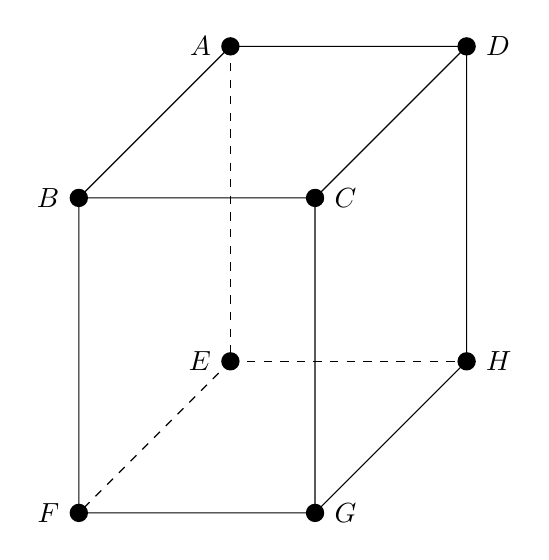
\begin{tikzpicture}[every edge quotes/.append style={auto, text=blue}]
				\pgfmathsetmacro{\cubex}{3}
				\pgfmathsetmacro{\cubey}{4}
				\pgfmathsetmacro{\cubez}{5}
				%%空間坐標中的CUBE 是以平面上的x軸 y軸再去擴充出深度z軸 z 往前為正,向後為負
				\coordinate (A) at (0,0,0);
				\coordinate (B) at (0,0,\cubez);
				\coordinate (C) at (\cubex, 0, \cubez );
				\coordinate (D) at (\cubex,0,0);
				\coordinate (E) at (0, -\cubey, 0);
				\coordinate (F) at (0, -\cubey, \cubez);
				\coordinate (G) at (\cubex, -\cubey, \cubez);
				\coordinate (H) at (\cubex, -\cubey, 0); 
				\draw [draw=black, every edge/.append style={draw=black, dashed}]
				(A) -- (B) --(C) --(D) -- cycle
				(C) -- (G) -- (H) -- (D) --cycle
				(B) -- (F) -- (G) -- (C) --cycle 
				(A) edge (E) 
				(E) edge (H)
				(E) edge (F);
				
				\foreach \v/\u/\t in 
				{A/180/$A$,
					B/180/$B$,
					C/0/$C$,
					D/0/$D$,
					E/180/$E$,
					F/180/$F$,
					G/0/$G$,
					H/0/$H$
				}
				{
					\draw[ultra thick,fill] (\v) circle (2.5pt);
					\node[label=\u:\t] at (\v){};
				};     
				\end{tikzpicture}
			\end{RightSidePic}
        \end{QBODY}
        \begin{QFROMS}
        \end{QFROMS}
        \begin{QTAGS}\QTAG{B4C1-2空間向量的坐標表示法}\QTAG{B4C1空間向量}\end{QTAGS}
        \begin{QANS}
            $\dfrac{4}{3}$
        \end{QANS}
        \begin{QSOLLIST}
            \begin{QSOL}
				\begin{LeftSide}[8cm]
					直角坐標坐標作法:\\
					\begin{QSTEPS}
						\QSTEP{ 令 $A(0,0,0), B(u,0,0), D(0,v,0), E(0,0,w) $}
						\QSTEP{ 由圖形可以知道平面$BDG$ 不會通過原點$A$,\\
							且與$x$, $y$, $z$ 軸皆有交點,且已知原平面過$B$, $D$ ,\\
							已有$x,y$ 截距,分別為 $u,v$\\
							可以假設 $E_{BDG}: \frac{x}{u} + \frac{y}{v} + \frac{z}{t} = 1$\\
							該平面通過$G(u,v,w)$ 代入可得:\\
							$1+1+\frac{w}{t}=1 \Rightarrow t= -w$\\
							$ \Rightarrow E_{BDG}: \frac{x}{u} + \frac{y}{v} + \frac{z}{-w} = 1 $
						}
						\QSTEP{ 由 $\lvec{AP} = \frac{1}{3} \lvec{AB} + 2 \lvec{AD} + a \lvec{AE} $\\
							可得點 $P$坐標為$ (\frac{1}{3} u, 2v, aw)$ \\
							且 $P$ 為平面 $BDG$ 上一點,\\
							代入滿足$E_{BDG}$ $\Rightarrow \frac{\frac{1}{3} u }{u}+\frac{2v}{v} + \frac{aw}{-w} = 1$ $\Rightarrow$\\
							 可解得 $a=\frac{4}{3}$ }
					\end{QSTEPS}
				\end{LeftSide}
				\begin{RightSidePic}
				   \begin{tikzpicture}
				   \pgfmathsetmacro{\cubex}{3}
				   \pgfmathsetmacro{\cubey}{4}
				   \pgfmathsetmacro{\cubez}{5}
				   %%空間坐標中的CUBE 是以平面上的x軸 y軸再去擴充出深度z軸 z 往前為正,向後為負
				   \coordinate (A) at (0,0,0);
				   \coordinate (B) at (0,0,\cubez);
				   
				   \coordinate (Bout) at (0,0,1.5*\cubez);
				   
				   \coordinate (C) at (\cubex, 0, \cubez );
				   \coordinate (D) at (\cubex,0,0);
				   
				   \coordinate (Dout) at (1.5*\cubex, 0, 0);
				   
				   \coordinate (E) at (0, -\cubey, 0);
				   
				   \coordinate (Eout) at (0, -\cubey *1.8, 0) ;
				   
				   \coordinate (F) at (0, -\cubey, \cubez);
				   \coordinate (G) at (\cubex, -\cubey, \cubez);
				   \coordinate (H) at (\cubex, -\cubey, 0); 
				   
				   \draw [draw=black, every edge/.append style={draw=black, dashed}]
				   (A) -- (B) --(C) --(D) -- cycle
				   (C) -- (G) -- (H) -- (D) --cycle
				   (B) -- (F) -- (G) -- (C) --cycle 
				   (A) edge (E) 
				   (E) edge (H)
				   (E) edge (F);
				   
				   \draw [fill=lightgray, opacity=0.5] (B)--(G)--(D) -- cycle;
				   
				   \draw[-{Stealth[scale=1.3,angle'=45]}, ultra thick] (A) -- (Dout) node[right] {$y$};
				   \draw[-{Stealth[scale=1.3,angle'=45]}, ultra thick] (A) -- (Bout) node[below] {$x$};
				   \draw[-{Stealth[scale=1.3,angle'=45]}, ultra thick] (A) -- (Eout) node[below] {$z$};
				   \foreach \v/\u/\t in 
				   {C/right/$C$,
					   F/left/$F$,
					   H/right/$H$
					}
					{
						\draw[ultra thick,fill] (\v) circle (2.5pt);
						\node[\u] at (\v){\t};
					};     
					\draw[ultra thick,fill] (A) circle (2.5pt);
					\draw[ultra thick,fill] (B) circle (2.5pt);
					\draw[ultra thick,fill] (D) circle (2.5pt);
					\draw[ultra thick,fill] (E) circle (2.5pt);
					\draw[ultra thick,fill] (G) circle (2.5pt);
					
					\node[above] at (A){$A(0,0,0)$};
					\node[label={[shift={(-1,0)}]$B(u,0,0)$} ] at (B) {};
					\node[above] at (D){$D(0,v,0)$};
					\node[right] at (G){$G(u,v,w)$};
					\node[label={[shift={(-1,0)}]$E(0,0,w)$}] at (E){};
					
					\end{tikzpicture}
				\end{RightSidePic}
			\end{QSOL}
\begin{QSOL}
			   \begin{LeftSide}[8cm]
			   採用向量坐標\\

				   \begin{QSTEPS}
					   \QSTEP{令 $\lvec{AB}, \lvec{AD}, \lvec{AE}$ 為基底向量,$A$ 為坐標原點 \\
						   可知:$B(1,0,0),D(0,1,0), G(1,1,1) , P(\frac{1}{3}, 2 , a)$ }
						\QSTEP{先計算 $E_{BDG}:$\\
							找法向量:$\lvec{BD} = (-1,1,0), \lvec{BG} = (0,1,1) $\\
							$\Rightarrow \lvec{BD}\times \lvec{BG} = (1,1,-1) $ \\
							取法向量為 $\lvec{n} =(1,1,-1)$\\
							找點:$G(1,1,1)$ \\
							$\Rightarrow E_{BDG}: x+y-z=1$
						}
						\QSTEP{$P\in E_{BDG}$,$P$ 點坐標代入可得\\ $\frac{1}{3} + 2-a =1 \Rightarrow a = \frac{4}{3}$ }
					\end{QSTEPS}
				\end{LeftSide}
			   \begin{RightSidePic}
				   \begin{tikzpicture}
				   \pgfmathsetmacro{\cubex}{3}
				   \pgfmathsetmacro{\cubey}{4}
				   \pgfmathsetmacro{\cubez}{5}
				   %%空間坐標中的CUBE 是以平面上的x軸 y軸再去擴充出深度z軸 z 往前為正,向後為負
				   \coordinate (A) at (0,0,0);
				   \coordinate (B) at (0,0,\cubez);
				   
				   \coordinate (Bout) at (0,0,1.5*\cubez);
				   
				   \coordinate (C) at (\cubex, 0, \cubez );
				   \coordinate (D) at (\cubex,0,0);
				   
				   \coordinate (Dout) at (1.5*\cubex, 0, 0);
				   
				   \coordinate (E) at (0, -\cubey, 0);
				   
				   \coordinate (Eout) at (0, -\cubey *1.8, 0) ;
				   
				   \coordinate (F) at (0, -\cubey, \cubez);
				   \coordinate (G) at (\cubex, -\cubey, \cubez);
				   \coordinate (H) at (\cubex, -\cubey, 0); 
				   
				   \draw [draw=black, every edge/.append style={draw=black, dashed}]
				   (A) -- (B) --(C) --(D) -- cycle
				   (C) -- (G) -- (H) -- (D) --cycle
				   (B) -- (F) -- (G) -- (C) --cycle 
				   (A) edge (E) 
				   (E) edge (H)
				   (E) edge (F);
				   
				   \draw [fill=lightgray, opacity=0.5] (B)--(G)--(D) -- cycle;
				   
				   \draw[-{Stealth[scale=1.3,angle'=45]}, ultra thick] (A) -- (Dout) node[right] {$y$};
				   \draw[-{Stealth[scale=1.3,angle'=45]}, ultra thick] (A) -- (Bout) node[below] {$x$};
				   \draw[-{Stealth[scale=1.3,angle'=45]}, ultra thick] (A) -- (Eout) node[below] {$z$};
				   \foreach \v/\u/\t in 
				   {C/right/$C$,
					   F/left/$F$,
					   H/right/$H$
					}
					{
						\draw[ultra thick,fill] (\v) circle (2.5pt);
						\node[\u] at (\v){\t};
					};     
					\draw[ultra thick,fill] (A) circle (2.5pt);
					\draw[ultra thick,fill] (B) circle (2.5pt);
					\draw[ultra thick,fill] (D) circle (2.5pt);
					\draw[ultra thick,fill] (E) circle (2.5pt);
					\draw[ultra thick,fill] (G) circle (2.5pt);
					
					\node[above] at (A){$A(0,0,0)$};
					\node[label={[shift={(-1,0)}]$B(1,0,0)$} ] at (B) {};
					\node[above] at (D){$D(0,1,0)$};
					\node[right] at (G){$G(1,1,1)$};
					\node[label={[shift={(-1,0)}]$E(0,0,1)$}] at (E){};
					
					\end{tikzpicture}
				\end{RightSidePic}
			\end{QSOL}
\begin{QSOL}
			   採用共面定理:\\
			   $\lvec{AP} 
			   = \frac{1}{3}\lvec{AB} + 2 \lvec{AD} + a(\lvec{AG} - \lvec {AB} -\lvec{AD} ) 
			   = (\frac{1}{3} - a) \lvec{AB} + (2-a) \lvec{AD} + a \lvec{AG} $
			   
			   根據共面定理可得:$(\frac{1}{3} - a) + (2-a) +a = 1 \Rightarrow a = \frac{4}{3} $\\
			   \vspace{1.5cm}\\
			   \psset{cornersize=absolute,linearc=.2\baselineskip} 
			   \psframebox[framesep=15pt]
			   {		
				   \begin{minipage}[c]{14cm}
					   共面定理:在空間坐標中,$O$ 與 $A,B,C$ 不共面, 有一點 $P$ \\
					   使得 $\lvec{OP} = \alpha \lvec{OA} +\beta \lvec{OB} +\gamma \lvec{OC} $ \\
					   若 $A,B,C,P$ 共面 ,則$\alpha+\beta+\gamma = 1$
					\end{minipage}
				}
			\end{QSOL}
\begin{QSOL}
			   採用共面定理:\\
			   $\lvec{AP} 
			   = \frac{1}{3}\lvec{AB} + 2 \lvec{AD} + a(\lvec{AG} - \lvec {AB} -\lvec{AD} ) 
			   = (\frac{1}{3} - a) \lvec{AB} + (2-a) \lvec{AD} + a \lvec{AG} $
			   
			   根據共面定理可得:$(\frac{1}{3} - a) + (2-a) +a = 1 \Rightarrow a = \frac{4}{3} $\\
			   
			   	   \begin{minipage}[c]{14cm}
					   共面定理:在空間坐標中,$O$ 與 $A,B,C$ 不共面, 有一點 $P$ \\
					   使得 $\lvec{OP} = \alpha \lvec{OA} +\beta \lvec{OB} +\gamma \lvec{OC} $ \\
					   若 $A,B,C,P$ 共面 ,則$\alpha+\beta+\gamma = 1$
					\end{minipage}
				
			\end{QSOL}

        \end{QSOLLIST}
        \begin{QEMPTYSPACE}
        \end{QEMPTYSPACE}
    \end{QUESTION}

% !TEX encoding = UTF-8 Unicode
% !TEX TS-program = xelatex 
\begin{QUESTIONS}
    \begin{QUESTION}
        \begin{ExamInfo}{106}{學測}{單選}{1}
        \end{ExamInfo}
        \begin{ExamAnsRateInfo}{53}{82}{52}{25}
        \end{ExamAnsRateInfo}
        \begin{QBODY}
            已知某校老師玩過「寶可夢」的比率為${{r}_{1}}$,而學生玩過的比率為${{r}_{2}}$,其中${{r}_{1}}\ne {{r}_{2}}$。
            由下列選項中的資訊,請選出可以判定全校師生玩過「寶可夢」的比率之選項。
            \begin{QOPS}
                \QOP 全校老師與學生比率     
                \QOP 全校老師人數
                \QOP 全校學生人數
                \QOP 全校師生人數
                \QOP 全校師生玩過「寶可夢」人數
            \end{QOPS}
        \end{QBODY}
        \begin{QFROMS}
        \end{QFROMS}
        \begin{QTAGS}\QTAG{B2C4數據分析}\QTAG{B2C4-1一維數據分析}\end{QTAGS}
        \begin{QANS}
            (1)
        \end{QANS}
        \begin{QSOLLIST}
        \end{QSOLLIST}
        \begin{QEMPTYSPACE}
        \end{QEMPTYSPACE}
    \end{QUESTION}
    \begin{QUESTION}
        \begin{ExamInfo}{106}{學測}{單選}{2}
        \end{ExamInfo}
        \begin{ExamAnsRateInfo}{51}{84}{52}{17}
        \end{ExamAnsRateInfo}
        \begin{QBODY}
            某個手機程式,每次點擊螢幕上的數$a$後,螢幕上的數會變成${{a}^{2}}$。當一開始時螢幕上的數$b$為正且連續點擊螢幕三次後,螢幕上的數接近${{81}^{3}}$。試問實數$b$最接近下列哪一個選項?
			\begin{QOPS}
				\QOP $1.7$      
				\QOP $3$      
				\QOP $5.2$      
				\QOP $9$      
				\QOP $81$
			\end{QOPS}
        \end{QBODY}
        \begin{QFROMS}
        \end{QFROMS}
        \begin{QTAGS}\QTAG{B1C3指對數函數}\QTAG{B1C3-1指數}\end{QTAGS}
        \begin{QANS}
            (3)
        \end{QANS}
        \begin{QSOLLIST}
        \end{QSOLLIST}
        \begin{QEMPTYSPACE}
        \end{QEMPTYSPACE}
    \end{QUESTION}
    \begin{QUESTION}
        \begin{ExamInfo}{106}{學測}{單選}{3}
        \end{ExamInfo}
        \begin{ExamAnsRateInfo}{38}{71}{34}{9}
        \end{ExamAnsRateInfo}
        \begin{QBODY}
            設$\Gamma :\frac{{{y}^{2}}}{{{a}^{2}}}-\frac{{{x}^{2}}}{{{b}^{2}}}=1$為坐標平面上一雙曲線,且其通過第一象限的漸近線為$\ell $。考慮動點$(t,{{t}^{2}})$,從時間$t=0$時出發。當$t>0$時,請選出正確的選項。
			\begin{QOPS}
			\QOP 此動點不會碰到$\Gamma $,也不會碰到$\ell $
			\QOP 此動點會碰到$\Gamma $,但不會碰到$\ell $
			\QOP 此動點會碰到$\ell $,但不會碰到$\Gamma $
			\QOP 此動點會先碰到$\Gamma $,再碰到$\ell $
			\QOP 此動點會先碰到$\ell $,再碰到$\Gamma $
			\end{QOPS}
        \end{QBODY}
        \begin{QFROMS}
        \end{QFROMS}
        \begin{QTAGS}\QTAG{B4C4二次曲線}\QTAG{B4C4-3雙曲線}\end{QTAGS}
        \begin{QANS}
            (5)
        \end{QANS}
        \begin{QSOLLIST}
        \end{QSOLLIST}
        \begin{QEMPTYSPACE}
        \end{QEMPTYSPACE}
    \end{QUESTION}
    \begin{QUESTION}
        \begin{ExamInfo}{106}{學測}{單選}{4}
        \end{ExamInfo}
        \begin{ExamAnsRateInfo}{55}{89}{60}{16}
        \end{ExamAnsRateInfo}
        \begin{QBODY}
            在右下圖的正立方體上有兩質點分別自頂點$A,C$同時出發,各自以等速直線運動分別向頂點$B,D$前進,且在1秒後分別同時到達$B,D$。請選出這段時間兩質點距離關係的正確選項。
        
			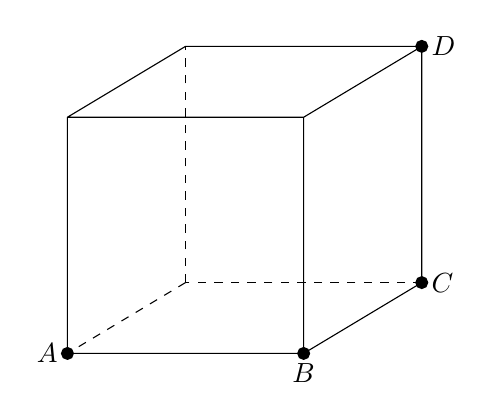
\begin{tikzpicture}[every edge quotes/.append style={auto, text=blue},
			x={(-0.25cm,-0.15cm)},
			y={(0.5cm,0cm)},
			z={(0cm,0.5cm)}]
			%%空間坐標中的CUBE 是以平面上的x軸 y軸再去擴充出深度z軸 z 往前為正,向後為負
			\coordinate (O) at (0,0,0);
			\coordinate (x) at (7,0,0);
			\coordinate (y) at 
			(0,7,0);
			\coordinate (z) at (0,0,7);
			
			\coordinate (Base1) at (0,0,0);
			\coordinate (Base2) at (6,0,0);
			\coordinate (Base3) at (6,6,0);
			\coordinate (Base4) at (0,6,0);
			\coordinate (Base1Up) at (0,0,6);
			\coordinate (Base2Up) at (6,0,6);
			\coordinate (Base3Up) at (6,6,6);
			\coordinate (Base4Up) at (0,6,6);
			
			\coordinate (A) at (Base2);
			\coordinate (B) at (Base3);
			\coordinate (C) at (Base4);
			\coordinate (D) at (Base4Up);
			
			\draw [draw=black, every edge/.append style={draw=black, dashed}]
			(Base1) edge (Base2)
			(Base2) -- (Base3)
			(Base3) -- (Base4)
			(Base4) edge (Base1)
			(Base1Up) -- (Base2Up)
			(Base2Up) -- (Base3Up)
			(Base3Up) -- (Base4Up)
			(Base4Up) -- (Base1Up)
			(Base1) edge (Base1Up)
			(Base2) -- (Base2Up)
			(Base3) -- (Base3Up)
			(Base4) -- (Base4Up);
			
			\foreach \v/\u/\t in 
			{ A/left/$A$,
				B/below/$B$,
				C/right/$C$,
				D/right/$D$
			}
			{
				\draw[ultra thick,fill] (\v) circle (1.5pt);
				\node[\u] at (\v){\t};
			}; 
			
			\end{tikzpicture}
			
			\begin{QOPS}
				\QOP 兩質點的距離固定不變
				\QOP 兩質點的距離越來越小
				\QOP 兩質點的距離越來越大
				\QOP 在$\frac{1}{2}$秒時兩質點的距離最小
				\QOP 在$\frac{1}{2}$秒時兩質點的距離最大
			\end{QOPS}
        \end{QBODY}
        \begin{QFROMS}
        \end{QFROMS}
        \begin{QTAGS}\QTAG{B4C1空間向量}\QTAG{B4C1-2空間向量的坐標表示法}\end{QTAGS}
        \begin{QANS}
            (4)
        \end{QANS}
        \begin{QSOLLIST}
        \end{QSOLLIST}
        \begin{QEMPTYSPACE}
        \end{QEMPTYSPACE}
    \end{QUESTION}
    \begin{QUESTION}
        \begin{ExamInfo}{106}{學測}{單選}{5}
        \end{ExamInfo}
        \begin{ExamAnsRateInfo}{37}{64}{35}{12}
        \end{ExamAnsRateInfo}
        \begin{QBODY}
            下圖是某城市在2016年的各月最低溫(橫軸$x$)與最高溫(縱軸$y$)的散佈圖。
            今以溫差(最高溫減最低溫)為橫軸且最高溫為縱軸重新繪製一散佈圖。試依此選出正確的選項。
			\begin{QOPS}
				\QOP 最高溫與溫差為正相關,且它們的相關性比最高溫與最低溫的相關性強
				\QOP 最高溫與溫差為正相關,且它們的相關性比最高溫與最低溫的相關性弱
				\QOP 最高溫與溫差為負相關,且它們的相關性比最高溫與最低溫的相關性強
				\QOP 最高溫與溫差為負相關,且它們的相關性比最高溫與最低溫的相關性弱
				\QOP 最高溫與溫差為零相關
			\end{QOPS}
        \end{QBODY}
        \begin{QFROMS}
        \end{QFROMS}
        \begin{QTAGS}\QTAG{B2C4數據分析}\QTAG{B2C4-2二維數據分析}\end{QTAGS}
        \begin{QANS}
            (4)
        \end{QANS}
        \begin{QSOLLIST}
        \end{QSOLLIST}
        \begin{QEMPTYSPACE}
        \end{QEMPTYSPACE}
    \end{QUESTION}
    \begin{QUESTION}
        \begin{ExamInfo}{106}{學測}{單選}{6}
        \end{ExamInfo}
        \begin{ExamAnsRateInfo}{22}{43}{16}{7}
        \end{ExamAnsRateInfo}
        \begin{QBODY}
            試問有多少個實數$x$滿足$\frac{\pi }{2}\le x\le \frac{3\pi }{2}$且$\cos x{}^\circ \le \cos x$?
			\begin{QOPS}
				\QOP $0$個     
				\QOP $1$個     
				\QOP $2$個     
				\QOP $4$個     
				\QOP 無窮多個
			\end{QOPS}
        \end{QBODY}
        \begin{QFROMS}
        \end{QFROMS}
        \begin{QTAGS}\QTAG{B3C1三角}\QTAG{B3C1-2廣義角與極坐標}\end{QTAGS}
        \begin{QANS}
            (1)
        \end{QANS}
        \begin{QSOLLIST}
        \end{QSOLLIST}
        \begin{QEMPTYSPACE}
        \end{QEMPTYSPACE}
    \end{QUESTION}
    \begin{QUESTION}
        \begin{ExamInfo}{106}{學測}{單選}{7}
        \end{ExamInfo}
        \begin{ExamAnsRateInfo}{29}{40}{27}{20}
        \end{ExamAnsRateInfo}
        \begin{QBODY}
            小明想要安排從星期一到星期五共五天的午餐計畫。他的餐點共有四種選擇:牛肉麵、大滷麵、咖哩飯及排骨飯。小明想要依據下列兩原則來安排他的午餐:
			(甲)每天只選一種餐點但這五天中每一種餐點至少各點一次
			(乙)連續兩天的餐點不能重複且不連續兩天吃麵食
			根據上述原則,小明這五天共有幾種不同的午餐計畫?
			\begin{QOPS}
				\QOP $52$      
				\QOP $60$      
				\QOP $68$      
				\QOP $76$      
				\QOP $84$
			\end{QOPS}
        \end{QBODY}
        \begin{QFROMS}
        \end{QFROMS}
        \begin{QTAGS}\QTAG{B2C2排列組合}\QTAG{B2C2-1簡單的邏輯與集合}\end{QTAGS}
        \begin{QANS}
            (2)
        \end{QANS}
        \begin{QSOLLIST}
        \end{QSOLLIST}
        \begin{QEMPTYSPACE}
        \end{QEMPTYSPACE}
    \end{QUESTION}
\end{QUESTIONS}
\begin{QUESTIONS}
    \begin{QUESTION}
        \begin{ExamInfo}{106}{學測}{多選}{8}
        \end{ExamInfo}
        \begin{ExamAnsRateInfo}{24}{35}{20}{17}
        \end{ExamAnsRateInfo}
        \begin{QBODY}
            設$m,n$為小於或等於4的相異正整數且$a,b$為非零實數。已知函數$f(x)=a{{x}^{m}}$與函數$g(x)=b{{x}^{n}}$的圖形恰有3個相異交點,請選出可能的選項。
			\begin{QOPS}
			\QOP $m,n$皆為偶數且$a,b$同號 
			\QOP $m,n$皆為偶數且$a,b$異號
			\QOP $m,n$皆為奇數且$a,b$同號
			\QOP $m,n$皆為奇數且$a,b$異號
			\QOP $m,n$為一奇一偶
			\end{QOPS}
        \end{QBODY}
        \begin{QFROMS}
        \end{QFROMS}
        \begin{QTAGS}\QTAG{B1C2多項式函數}\QTAG{B1C2-4多項式函數圖形與多項式不等式}\end{QTAGS}
        \begin{QANS}
            (1)(3)
        \end{QANS}
        \begin{QSOLLIST}
        \end{QSOLLIST}
        \begin{QEMPTYSPACE}
        \end{QEMPTYSPACE}
    \end{QUESTION}
    \begin{QUESTION}
        \begin{ExamInfo}{106}{學測}{多選}{9}
        \end{ExamInfo}
        \begin{ExamAnsRateInfo}{34}{57}{30}{15}
        \end{ExamAnsRateInfo}
        \begin{QBODY}
            設$\Gamma $為坐標平面上的圓,點$(0,0)$在$\Gamma $的外部且點$(2,6)$在$\Gamma $的內部。請選出正確的選項。
			\begin{QOPS}
			\QOP $\Gamma $的圓心不可能在第二象限
			\QOP $\Gamma $的圓心可能在第三象限且此時$\Gamma $的半徑必定大於10
			\QOP $\Gamma $的圓心可能在第一象限且此時$\Gamma $的半徑必定小於10
			\QOP $\Gamma $的圓心可能在$x$軸上且此時圓心的$x$坐標必定小於10
			\QOP $\Gamma $的圓心可能在第四象限且此時$\Gamma $的半徑必定大於10
			\end{QOPS}
        \end{QBODY}
        \begin{QFROMS}
        \end{QFROMS}
        \begin{QTAGS}\QTAG{B3C2直線與圓}\QTAG{B3C2-3圓與直線的關係}\end{QTAGS}
        \begin{QANS}
            (5)
        \end{QANS}
        \begin{QSOLLIST}
        \end{QSOLLIST}
        \begin{QEMPTYSPACE}
        \end{QEMPTYSPACE}
    \end{QUESTION}
    \begin{QUESTION}
        \begin{ExamInfo}{106}{學測}{多選}{10}
        \end{ExamInfo}
        \begin{ExamAnsRateInfo}{43}{66}{39}{24}
        \end{ExamAnsRateInfo}
        \begin{QBODY}
            坐標空間中有三直線${{L}_{1}}:\dfrac{x-1}{2}=\dfrac{y+1}{2}=\dfrac{z}{1},{{L}_{2}}:\left\{ \begin{aligned}
			& x-2y+2z=-4 \\ 
			& x+y-4z=5 \\ 
			\end{aligned} \right.,{{L}_{3}}:\left\{ \begin{aligned}
			& x=-t \\ 
			& y=-2-t \\ 
			& z=4+4t \\ 
			\end{aligned} \right.$,$t$為實數。請選出正確的選項。
			\begin{QOPS}
				\QOP ${{L}_{1}}$與${{L}_{2}}$的方向向量互相垂直
				\QOP ${{L}_{1}}$與${{L}_{3}}$的方向向量互相垂直
				\QOP 有一個平面同時包含${{L}_{1}}$與${{L}_{2}}$
				\QOP 有一個平面同時包含${{L}_{1}}$與${{L}_{3}}$
				\QOP 有一個平面同時包含${{L}_{2}}$與${{L}_{3}}$
			\end{QOPS}
        \end{QBODY}
        \begin{QFROMS}
        \end{QFROMS}
        \begin{QTAGS}\QTAG{B4C2空間中的平面與直線}\QTAG{B4C2-2空間直線方程式}\end{QTAGS}
        \begin{QANS}
            (2)(3)(4)
        \end{QANS}
        \begin{QSOLLIST}
        \end{QSOLLIST}
        \begin{QEMPTYSPACE}
        \end{QEMPTYSPACE}
    \end{QUESTION}
    \begin{QUESTION}
        \begin{ExamInfo}{106}{學測}{多選}{11}
        \end{ExamInfo}
        \begin{ExamAnsRateInfo}{62}{84}{64}{38}
        \end{ExamAnsRateInfo}
        \begin{QBODY}
            設最近數學家發現一種新的可以無縫密舖平面的凸五邊形$ABCDE$,其示意圖如下。關於這五邊形,請選出正確的選項。
			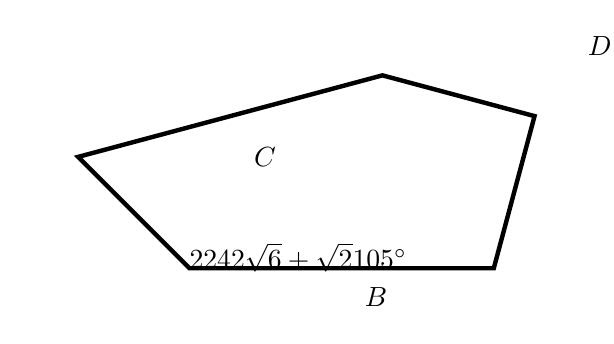
\begin{tikzpicture}[scale=1.0]
				\coordinate (B) at (0,0);
				\coordinate (A) at (0:{sqrt(6)+sqrt(2)});
				\path (A) ++(75:2) coordinate (E);
				\path (E) ++(165:2) coordinate (D);
				\coordinate (C) at (135:2);
				
				
				\draw[ultra thick] (A) -- (B)--(C)--(D)--(E) --cycle;
				\tkzLabelSegment[midway,  right](E,A){$2$};
				\tkzLabelSegment[midway,  above](D,E){$2$};
				\tkzLabelSegment[midway,  above](D,C){$4$};
				\tkzLabelSegment[midway,  below left](C,B){$2$};
				\tkzLabelSegment[midway,  below](B,A){$\sqrt{6}+\sqrt{2}$};
				\tkzMarkRightAngle[size=0.3](D,E,A);
				\tkzMarkAngle[size=0.3](E,A,B);
				\tkzLabelAngle[pos=0.6](E,A,B){$105^\circ$};
				
				\node[label=315:$A$] at (A){};
				\node[label=225:$B$] at (B){};
				\node[label=180:$C$] at (C){};
				\node[label=90:$D$] at (D){};
				\node[label=45:$E$] at (E){};
			\end{tikzpicture}
			\begin{QOPS}
			\QOP $\overline{AD}=2\sqrt[{}]{2}$
			\QOP $\angle DAB=45{}^\circ $
			\QOP $\overline{BD}=2\sqrt[{}]{6}$
			\QOP $\angle ABD=45{}^\circ $
			\QOP $BCD$的面積為$2\sqrt[{}]{2}$
			\end{QOPS}
        \end{QBODY}
        \begin{QFROMS}
        \end{QFROMS}
        \begin{QTAGS}\QTAG{B3C1三角}\QTAG{B3C1-3正弦定理與餘弦定理}\end{QTAGS}
        \begin{QANS}
            (1)(4)
        \end{QANS}
        \begin{QSOLLIST}
        \end{QSOLLIST}
        \begin{QEMPTYSPACE}
        \end{QEMPTYSPACE}
    \end{QUESTION}
    \begin{QUESTION}
        \begin{ExamInfo}{106}{學測}{多選}{12}
        \end{ExamInfo}
        \begin{ExamAnsRateInfo}{28}{37}{27}{20}
        \end{ExamAnsRateInfo}
        \begin{QBODY}
            某班級50位學生,段考國文、英文、數學及格的人數分別為45、39、34人,且英文及格的學生國文也都及格。現假設數學和英文皆及格的有$x$人,數學及格但英文不及格的有$y$人。請選出正確的選項。
			\begin{QOPS}
				\QOP $x+y=39$
				\QOP $y\le 11$
				\QOP 三科中至少有一科不及格的學生有$39-x+y$人
				\QOP 三科中至少有一科不及格的學生最少有11人
				\QOP 三科中至少有一科不及格的學生最多有27人
			\end{QOPS}
        \end{QBODY}
        \begin{QFROMS}
        \end{QFROMS}
        \begin{QTAGS}\QTAG{B2C2排列組合}\QTAG{B2C2-1簡單的邏輯與集合}\end{QTAGS}
        \begin{QANS}
            (2)(5)
        \end{QANS}
        \begin{QSOLLIST}
            \begin{QSOL}
				\begin{QSTEPS}
					\QSTEP{ 令全班為集合$U$,國文、數學、英文,及格的集合分別為 $C,M,E$ \\
							可得:$n(C) = 45, n(M) = 34 , n(E) = 39$}
					\QSTEP{ $x+y = n (M \cap E) + n (M \cap \overline{E}) = n(M) = 34$,則 (1) 錯誤}
					\QSTEP{ $n(\bar{E}) = 50 -39 =11 \ge n (M \cap \bar{E}) \Rightarrow y \le 11$,則 (2) 正確}
					\QSTEP{ 由以上兩步驟可得 $23 \le x\le 34$}
					\QSTEP{ 至少一科不及格 $= n(\text{全}) - n (C\cap M\cap E) = 50-x$,\\
							可得 $16 \le \text{至少一科不及格} \le 27$}
				\end{QSTEPS}
				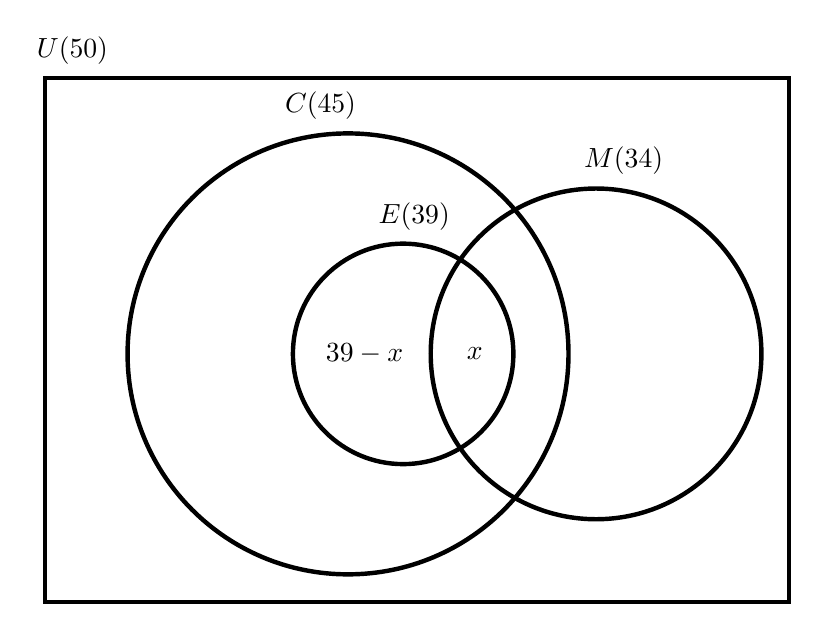
\begin{tikzpicture}[scale=0.7]
					\draw[ultra thick]  (-6.5,6) circle (2);
					\draw[ultra thick]  (-7.5,6) node (v1) {} ellipse (4 and 4);
					\draw[ultra thick]  (-3,6) node (v2) {} circle (3);
					\draw[ultra thick]  (-13,11) rectangle (0.5,1.5);
					\node at (-12.5,11.5) {$U(50)$};
					\node at (-8,10.5) {$C(45)$};
					\node at (-5.2,6) {$x$};
					\node at (-7.2,6) {$39-x$};
					\node at (-6.3,8.5) {$E(39)$};
					\node at (-2.5,9.5) {$M(34)$};
				\end{tikzpicture}
			\end{QSOL}
        \end{QSOLLIST}
        \begin{QEMPTYSPACE}
        \end{QEMPTYSPACE}
    \end{QUESTION}
    \begin{QUESTION}
        \begin{ExamInfo}{106}{學測}{多選}{13}
        \end{ExamInfo}
        \begin{ExamAnsRateInfo}{36}{54}{32}{22}
        \end{ExamAnsRateInfo}
        \begin{QBODY}
            空間中有一四面體$ABCD$。假設$\lvec{AD}$分別與$\lvec{AB}$和$\lvec{AC}$垂直,請選出正確的選項。
			\begin{QOPS}
				\QOP $\lvec{DB}\cdot\lvec{DC} ={{\overline{DA}}^{2}}- \lvec{AB}\cdot \lvec{AC}$
				\QOP 若$\angle BAC$是直角,則$\angle BDC$是直角
				\QOP 若$\angle BAC$是銳角,則$\angle BDC$是銳角
				\QOP 若$\angle BAC$是鈍角,則$\angle BDC$是鈍角
				\QOP 若$\overline{AB}<\overline{DA}$且$\overline{AC}<\overline{DA}$,則$\angle BDC$是銳角
			\end{QOPS}
        \end{QBODY}
        \begin{QFROMS}
        \end{QFROMS}
        \begin{QTAGS}\QTAG{B4C1空間向量}\QTAG{B4C1-3空間向量的內積}\end{QTAGS}
        \begin{QANS}
            (3)(5)
        \end{QANS}
        \begin{QSOLLIST}
        \end{QSOLLIST}
        \begin{QEMPTYSPACE}
        \end{QEMPTYSPACE}
    \end{QUESTION}
\end{QUESTIONS}
\begin{QUESTIONS}
    \begin{QUESTION}
        \begin{ExamInfo}{106}{學測}{填充}{A}
        \end{ExamInfo}
        \begin{ExamAnsRateInfo}{54}{82}{60}{20}
        \end{ExamAnsRateInfo}
        \begin{QBODY}
            遞迴數列$\langle {{a}_{n}}\rangle $滿足${{a}_{n}}={{a}_{n-1}}+f(n-2)$,其中$n\ge 2$且$f(x)$為二次多項式。若${{a}_{1}}=1,{{a}_{2}}=2,{{a}_{3}}=5,{{a}_{4}}=12$,則${{a}_{5}}= \TCNBOX{ \TCN\TCN }$     。
        \end{QBODY}
        \begin{QFROMS}
        \end{QFROMS}
        \begin{QTAGS}\QTAG{B2C1數列級數}\QTAG{B2C1-1數列}\end{QTAGS}
        \begin{QANS}
            $25$
        \end{QANS}
        \begin{QSOLLIST}
        \end{QSOLLIST}
        \begin{QEMPTYSPACE}
        \end{QEMPTYSPACE}
    \end{QUESTION}
    \begin{QUESTION}
        \begin{ExamInfo}{106}{學測}{填充}{B}
        \end{ExamInfo}
        \begin{ExamAnsRateInfo}{26}{65}{12}{1}
        \end{ExamAnsRateInfo}
        \begin{QBODY}
            坐標平面上,$ABC$內有一點$P$滿足$\lvec{AP}=(\frac{4}{3},\frac{5}{6})$及$\lvec{AP}=\frac{1}{2}\lvec{AB}+\frac{1}{5}\lvec{AC}$。若$A,P$連線交$\overline{BC}$於$M$,則$\lvec{AM}= \TCNBOX{\left(\FR{\TCN\TCN}{\TCN\TCN} ,\FR{\TCN\TCN}{\TCN\TCN} \right)}$。(化成最簡分數)
        \end{QBODY}
        \begin{QFROMS}
        \end{QFROMS}
        \begin{QTAGS}\QTAG{B3C3平面向量}\QTAG{B3C3-1平面向量的表示法}\end{QTAGS}
        \begin{QANS}
            $(\dfrac{40}{21},\dfrac{25}{21})$
        \end{QANS}
        \begin{QSOLLIST}
        \end{QSOLLIST}
        \begin{QEMPTYSPACE}
        \end{QEMPTYSPACE}
    \end{QUESTION}
    \begin{QUESTION}
        \begin{ExamInfo}{106}{學測}{填充}{C}
        \end{ExamInfo}
        \begin{ExamAnsRateInfo}{30}{63}{22}{5}
        \end{ExamAnsRateInfo}
        \begin{QBODY}
            若$a$為正整數且方程式$5{{x}^{3}}+(a+4){{x}^{2}}+ax+1=0$的根都是有理根,則$a= \TCNBOX{\TCN}$     。
        \end{QBODY}
        \begin{QFROMS}
        \end{QFROMS}
        \begin{QTAGS}\QTAG{B1C2多項式函數}\QTAG{B1C2-3多項式方程式}\end{QTAGS}
        \begin{QANS}
            $7$
        \end{QANS}
        \begin{QSOLLIST}
        \end{QSOLLIST}
        \begin{QEMPTYSPACE}
        \end{QEMPTYSPACE}
    \end{QUESTION}
    \begin{QUESTION}
        \begin{ExamInfo}{106}{學測}{填充}{D}
        \end{ExamInfo}
        \begin{ExamAnsRateInfo}{37}{70}{33}{8}
        \end{ExamAnsRateInfo}
        \begin{QBODY}
            設${{a}_{1}},{{a}_{2}},\cdots ,{{a}_{9}}$為等差數列且$k$為實數。若方程組
			$\left\{ \begin{aligned}
			& {{a}_{1}}x-{{a}_{2}}y+2{{a}_{3}}z=k+1 \\ 
			& {{a}_{4}}x-{{a}_{5}}y+2{{a}_{6}}z=-k-5 \\ 
			& {{a}_{7}}x-{{a}_{8}}y+2{{a}_{9}}z=k+9 \\ 
			\end{aligned} \right.$有解,
			則$k=\TCNBOX{\TCN\TCN}$      。
        \end{QBODY}
        \begin{QFROMS}
        \end{QFROMS}
        \begin{QTAGS}\QTAG{B4C3矩陣}\QTAG{B4C3-1線性方程組與矩陣}\end{QTAGS}
        \begin{QANS}
            $-5$
        \end{QANS}
        \begin{QSOLLIST}
        \end{QSOLLIST}
        \begin{QEMPTYSPACE}
        \end{QEMPTYSPACE}
    \end{QUESTION}
    \begin{QUESTION}
        \begin{ExamInfo}{106}{學測}{填充}{E}
        \end{ExamInfo}
        \begin{ExamAnsRateInfo}{24}{59}{12}{1}
        \end{ExamAnsRateInfo}
        \begin{QBODY}
            設$a,b,x$皆為正整數且滿足$a\le x\le b$及$b-a=3$。若用內插法從$\log a,\log b$求得$\log x$的
			近似值為
			$\log x\approx \frac{1}{3}\log a+\frac{2}{3}\log b=\frac{1}{3}(1+2\log 3-\log 2)+\frac{2}{3}(4\log 2+\log 3)$,
			則$x$的值為 $\TCNBOX{\TCN\TCN}$        。
        \end{QBODY}
        \begin{QFROMS}
        \end{QFROMS}
        \begin{QTAGS}\QTAG{B1C3指對數函數}\QTAG{B1C3-5指數與對數的應用}\end{QTAGS}
        \begin{QANS}
            $47$
        \end{QANS}
        \begin{QSOLLIST}
        \end{QSOLLIST}
        \begin{QEMPTYSPACE}
        \end{QEMPTYSPACE}
    \end{QUESTION}
    \begin{QUESTION}
        \begin{ExamInfo}{106}{學測}{填充}{F}
        \end{ExamInfo}
        \begin{ExamAnsRateInfo}{19}{45}{11}{1}
        \end{ExamAnsRateInfo}
        \begin{QBODY}
            一隻青蛙位於坐標平面的原點,每步隨機朝上、下、左、右跳一單位長,總共跳了四步。青蛙跳了四步後恰回到原點的機率為$\TCNBOX{\FR{\TCN}{\TCN\TCN}}$。(化成最簡分數)
        \end{QBODY}
        \begin{QFROMS}
        \end{QFROMS}
        \begin{QTAGS}\QTAG{B2C3機率}\QTAG{B2C3-2機率的定義與性質}\end{QTAGS}
        \begin{QANS}
            $\dfrac{9}{64}$
        \end{QANS}
        \begin{QSOLLIST}
        \end{QSOLLIST}
        \begin{QEMPTYSPACE}
        \end{QEMPTYSPACE}
    \end{QUESTION}
    \begin{QUESTION}
        \begin{ExamInfo}{106}{學測}{填充}{G}
        \end{ExamInfo}
        \begin{ExamAnsRateInfo}{22}{56}{9}{1}
        \end{ExamAnsRateInfo}
        \begin{QBODY}
            地面上甲、乙兩人從同一地點同時開始移動。甲以每秒4公尺向東等速移動,乙以每秒3公尺向北等速移動。在移動不久之後,他們互望的視線被一圓柱體 建築物阻擋了6秒後才又相見。此圓柱體建築物底圓的直徑為$\TCNBOX{\TCN\TCN.\TCN}$公尺。
        \end{QBODY}
        \begin{QFROMS}
        \end{QFROMS}
        \begin{QTAGS}\QTAG{B3C2直線與圓}\QTAG{B3C2-3圓與直線的關係}\end{QTAGS}
        \begin{QANS}
            $14.4$
        \end{QANS}
        \begin{QSOLLIST}
        \end{QSOLLIST}
        \begin{QEMPTYSPACE}
        \end{QEMPTYSPACE}
    \end{QUESTION}
\end{QUESTIONS}


\clearpage
\setcounter{page}{1}
\cfoot{}
%\cfoot{陳立教育 -答案卷\thepage- 絕對智慧 }%中間 footer 擺放頁碼
%\input{AnswerPage.tex}
%\newpage
\clearpage
\setcounter{page}{1}
\cfoot{陳立教育 -解\thepage- 絕對智慧 }%中間 footer 擺放頁碼
%詳解區抬頭
% !TEX encoding = UTF-8 Unicode
% !TEX TS-program = xelatex
%詳解區抬頭
\psset{cornersize=absolute,linearc=.5\baselineskip} 
\psframebox[framesep=10pt]
{		
    \begin{minipage}[c]{16cm}
        {
            \fontsize{22}{22}
            \makebox[\textwidth][s]{\ChenLi \classNameString \yearString  \numForQuizTitle } \par  
           }
    \end{minipage}
}

%正式詳解區:
\def\FlagShowAnswer{1}  %設定顯現 QANS environment 裡面的資料
\def\FlagShowSolution{1} %設定顯現 QSOL environment 裡面的資料
\def\FlagShowTAG{1}
\def\FlagAddSolutionBox{0}
%設定三大題區塊

\vspace{1cm}

% !TEX encoding = UTF-8 Unicode
% !TEX TS-program = xelatex 
\begin{QUESTIONS}
    \begin{QUESTION}
        \begin{ExamInfo}{091}{學測}{單選}{1}
        \end{ExamInfo}
        \begin{ExamAnsRateInfo}{76}{97}{83}{48}
        \end{ExamAnsRateInfo}
        \begin{QBODY}
            設 $P(x,y)$ 為坐標平面上一點,且滿足
            $(x-1)^2 +(y-2)^2 + (x-3)^2 +(y-4)^2 = (3-1)^2 +(4-2)^2$
            ,那麼 $P$ 點的位置在哪裡?
            
            \begin{QOPS} 
                \QOP 第一象限 
                \QOP 第二象限 
                \QOP 第三象限 
                \QOP 第四象限 
                \QOP $x$ 軸或 $y$ 軸上
            \end{QOPS}
        \end{QBODY}
        \begin{QFROMS}
        \end{QFROMS}
        \begin{QTAGS}\QTAG{B4C4二次曲線}\end{QTAGS}
        \begin{QANS}
            (1)
        \end{QANS}
        \begin{QSOLLIST}
        \end{QSOLLIST}
        \begin{QEMPTYSPACE}
        \end{QEMPTYSPACE}
    \end{QUESTION}
    \begin{QUESTION}
        \begin{ExamInfo}{091}{學測}{單選}{2}
        \end{ExamInfo}
        \begin{ExamAnsRateInfo}{51}{79}{51}{23}
        \end{ExamAnsRateInfo}
        \begin{QBODY}
            一群登山友,在山上發現一顆巨樹,隊中 $10$ 位身高 $170$ 公分的男生,手拉著手剛好環抱大樹一 圈。問樹幹的直徑最接近下列何值? 
            \begin{QOPS} 
                \QOP $3$公尺 
                \QOP $5$公尺
                \QOP $7$公尺 
                \QOP $9$公尺 
                \QOP $11$ 公尺
            \end{QOPS}
        \end{QBODY}
        \begin{QFROMS}
        \end{QFROMS}
        \begin{QTAGS}\QTAG{綜合}\end{QTAGS}
        \begin{QANS}
            (2)
        \end{QANS}
        \begin{QSOLLIST}
        \end{QSOLLIST}
        \begin{QEMPTYSPACE}
        \end{QEMPTYSPACE}
    \end{QUESTION}
    \begin{QUESTION}
        \begin{ExamInfo}{091}{學測}{單選}{3}
        \end{ExamInfo}
        \begin{ExamAnsRateInfo}{62}{94}{65}{27}
        \end{ExamAnsRateInfo}
        \begin{QBODY}
            如圖,下面哪一選項中的向量與另兩個向量 $\lvec{PO}$, $\lvec{QO}$ 之和等於零向量?
            \begin{QOPS} 
                \QOP $\lvec{AO}$ 
                \QOP $\lvec{BO}$ 
                \QOP $\lvec{CO}$ 
                \QOP $\lvec{DO}$ 
                \QOP $\lvec{EO}$ 
            \end{QOPS}

                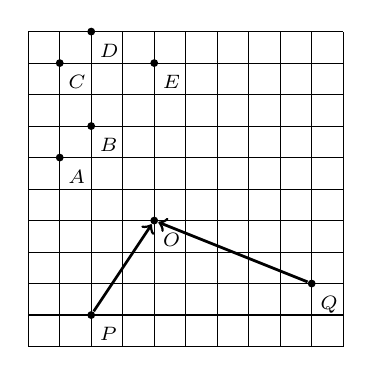
\begin{tikzpicture}[scale=.4]
                \draw (0,0) grid (10,10);\scriptsize
                \foreach \v/\x/\y in {P/2/1,Q/9/2,O/4/4,A/1/6,B/2/7,C/1/9,D/2/10,E/4/9}
                \node[fill,inner sep=1pt,circle] (v\v) at (\x,\y)[label=280:$\v$] {};
                \foreach \i/\j in {P/O, Q/O}
                \draw[->,line width=1pt] (v\i) to (v\j);
                \end{tikzpicture}

        \end{QBODY}
        \begin{QFROMS}
        \end{QFROMS}
        \begin{QTAGS}\QTAG{B3C3平面向量}\end{QTAGS}
        \begin{QANS}
            (3)
        \end{QANS}
        \begin{QSOLLIST}
        \end{QSOLLIST}
        \begin{QEMPTYSPACE}
        \end{QEMPTYSPACE}
    \end{QUESTION}
    \begin{QUESTION}
        \begin{ExamInfo}{091}{學測}{單選}{4}
        \end{ExamInfo}
        \begin{ExamAnsRateInfo}{35}{60}{27}{18}
        \end{ExamAnsRateInfo}
        \begin{QBODY}
            若某校 $1000$ 位學生的數學段考成績平均分數是 $65.24$ 分,樣本標準差是 $5.24$ 分,而且已知成績分佈呈現常態分配。試問全校約有多少人數學成績低於 $60$ 分?
            \begin{QOPS}
                \QOP 約$80$人  
                \QOP 約$160$人 
                \QOP 約$240$人 
                \QOP 約$320$人 
                \QOP 約$400$人
            \end{QOPS}
        \end{QBODY}
        \begin{QFROMS}
        \end{QFROMS}
        \begin{QTAGS}\QTAG{B5C1機率與統計}\end{QTAGS}
        \begin{QANS}
            (2)
        \end{QANS}
        \begin{QSOLLIST}
        \end{QSOLLIST}
        \begin{QEMPTYSPACE}
        \end{QEMPTYSPACE}
    \end{QUESTION}
    \begin{QUESTION}
        \begin{ExamInfo}{091}{學測}{單選}{5}
        \end{ExamInfo}
        \begin{ExamAnsRateInfo}{52}{82}{54}{20}
        \end{ExamAnsRateInfo}
        \begin{QBODY}
            試問用下列哪一個函數的部分圖形來描述右圖較恰當?
            \begin{QOPS}
            \QOP $(x-2)^{2}-2$  
            \QOP $2\sin(x)+2$
            \QOP $2\cos(x)$ 
            \QOP $-0.5(x-2)^{2}+4$ 
            \QOP $3-2^{x}$ 
            \end{QOPS}
            \begin{tikzpicture}[scale=.5]
                \begin{scope}\scriptsize
                \draw[->] (0,-1) to (0,5) node[above] {$y$};
                \draw[->] (-1,0) to (5,0) node[right] {$x$};
                \node[] at (1,-.6) {$(1,0)$};
                \node[] at (-1,1) {$(0,1)$};
                \node[draw,fill,circle,inner sep=1pt] at (0,1) {};
                \node[draw,fill,circle,inner sep=1pt] at (1,0) {};
                \draw[smooth,samples=100,domain=0:5] plot(\x,{-.5*(\x-2)*(\x-2)+4});
                %\draw[smooth,samples=100] (3,3) ellipse (2cm and 4cm) ;
                \end{scope}
            \end{tikzpicture}
        \end{QBODY}
        \begin{QFROMS}
        \end{QFROMS}
        \begin{QTAGS}\QTAG{綜合}\end{QTAGS}
        \begin{QANS}
            (4)
        \end{QANS}
        \begin{QSOLLIST}
        \end{QSOLLIST}
        \begin{QEMPTYSPACE}
        \end{QEMPTYSPACE}
    \end{QUESTION}
    \begin{QUESTION}
        \begin{ExamInfo}{091}{學測}{單選}{6}
        \end{ExamInfo}
        \begin{ExamAnsRateInfo}{33}{53}{32}{14}
        \end{ExamAnsRateInfo}
        \begin{QBODY}
            在坐標平面上有一橢圓,它的長軸落在 $x$ 軸上,短軸落在 $y$ 軸上,長軸、短軸的長度分別為 $4$、$2$。
            如圖所示,通過橢圓的中心 $O$ 且與 $x$ 軸夾角為 $45$ 度的直線在第一象限跟橢圓相交於 $P$。 則此交點 $P$ 與中心 $O$ 的距離為 
            
            
            \begin{QOPS} 
                \QOP $1.5$
                \QOP $\sqrt{1.6}$ 
                \QOP $\sqrt{2}$ 
                \QOP $\sqrt{2.5}$ 
                \QOP $
                \sqrt{3.2}$
            \end{QOPS}
        
            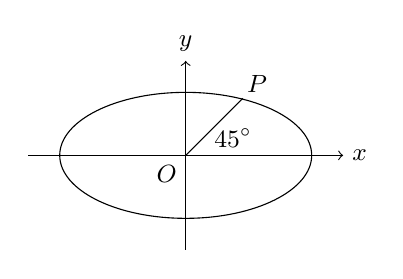
\begin{tikzpicture}[scale=.8]
            \begin{scope}\small
            \draw[->] (0,-1.5) to (0,1.5) node[above] {$y$};
            \draw[->] (-2.5,0) to (2.5,0) node[right] {$x$};
            \node (vO) at (-.3,-.3) {$O$};
            %\draw[smooth,samples=100,domain=.5:2.5] (plot(\x,{2.3*sqrt(\x-.5)});
            \draw (0,0) to (45:1.28);
            \node (vP) at (45:1.6) {$P$};
            \node (vP) at (20:.8) {$45^{\circ}$};
            \draw[smooth,samples=100] (0,0) ellipse (2cm and 1cm) ;
            \end{scope}
            \end{tikzpicture}
            
        \end{QBODY}
        \begin{QFROMS}
        \end{QFROMS}
        \begin{QTAGS}\QTAG{B4C4二次曲線}\end{QTAGS}
        \begin{QANS}
            (2)
        \end{QANS}
        \begin{QSOLLIST}
        \end{QSOLLIST}
        \begin{QEMPTYSPACE}
        \end{QEMPTYSPACE}
    \end{QUESTION}
\end{QUESTIONS}
\begin{QUESTIONS}
    \begin{QUESTION}
        \begin{ExamInfo}{091}{學測}{多選}{7}
        \end{ExamInfo}
        \begin{ExamAnsRateInfo}{75}{93}{82}{50}
        \end{ExamAnsRateInfo}
        \begin{QBODY}
            若實數 $a,b,c$ 滿足 $abc>0$, $ab+bc+ca<0$, $a+b+c>0$, $a>b>c$ ,則下列選項何者為真? 
            \begin{QOPS} 
                \QOP $a>0$ 
                \QOP $b>0$ 
                \QOP $c>0$
                \QOP $|a|>|b|$ 
                \QOP $a^2>c^2$
            \end{QOPS}
        \end{QBODY}
        \begin{QFROMS}
        \end{QFROMS}
        \begin{QTAGS}\QTAG{綜合}\end{QTAGS}
        \begin{QANS}
            (1)(4)(5)
        \end{QANS}
        \begin{QSOLLIST}
        \end{QSOLLIST}
        \begin{QEMPTYSPACE}
        \end{QEMPTYSPACE}
    \end{QUESTION}
    \begin{QUESTION}
        \begin{ExamInfo}{091}{學測}{多選}{8}
        \end{ExamInfo}
        \begin{ExamAnsRateInfo}{60}{88}{64}{28}
        \end{ExamAnsRateInfo}
        \begin{QBODY}
            一機器狗每秒鐘前進或者後退一步,程式設計師讓機器狗以前進 $3$ 步,然後再後退 $2$ 步的規律移動。如果將此機器狗放在數線的原點,面向正的方向,以 $1$ 步的距離為 $1$ 單位長。令 $P(n)$ 表示第 $n$ 秒時機器狗所在位置的坐標,且 $P(0)=0$。那麼下列選項何者為真? 
            \begin{QOPS}
                \QOP $P(3)=3$ 
                \QOP $P(5)=1$ 
                \QOP $P(10)=2$
                \QOP $P(101)=21$ 
                \QOP $P(103)<P(104)$
            \end{QOPS}
        \end{QBODY}
        \begin{QFROMS}
        \end{QFROMS}
        \begin{QTAGS}\QTAG{B2C1數列級數}\end{QTAGS}
        \begin{QANS}
            (1)(2)(3)(4)
        \end{QANS}
        \begin{QSOLLIST}
        \end{QSOLLIST}
        \begin{QEMPTYSPACE}
        \end{QEMPTYSPACE}
    \end{QUESTION}
    \begin{QUESTION}
        \begin{ExamInfo}{091}{學測}{多選}{9}
        \end{ExamInfo}
        \begin{ExamAnsRateInfo}{31}{53}{26}{14}
        \end{ExamAnsRateInfo}
        \begin{QBODY}
            下列哪些選項與方程組 $\left\{ \begin{array}{l} 2x+y+3z=0 \\ 4x+3y+6z =0 \end{array}\right.$ 的解集合相同?
            
            \begin{QOPS} 
                \QOP $y=0$ 
                
                \QOP 
                $\left\{ \begin{array}{l} 2x+3z=0 \\y=0 \end{array}\right.$
                
                \QOP
                $x=y=0$
                
                \QOP
                $\left\{ \begin{array}{l} x+\frac{1}{2}y+\frac{3}{2}z=0 \\ 4x+3y+6z =0 \end{array}\right.$
                
                \QOP
                $\left\{ \begin{array}{l} 6x+4y+9z=0 \\ 2x+y+3z =0 \end{array}\right.$
            \end{QOPS}
        \end{QBODY}
        \begin{QFROMS}
        \end{QFROMS}
        \begin{QTAGS}\QTAG{B4C3矩陣}\end{QTAGS}
        \begin{QANS}
            (2)(4)(5)
        \end{QANS}
        \begin{QSOLLIST}
        \end{QSOLLIST}
        \begin{QEMPTYSPACE}
        \end{QEMPTYSPACE}
    \end{QUESTION}
    \begin{QUESTION}
        \begin{ExamInfo}{091}{學測}{多選}{10}
        \end{ExamInfo}
        \begin{ExamAnsRateInfo}{20}{40}{11}{9}
        \end{ExamAnsRateInfo}
        \begin{QBODY}
            觀察相關的函數圖形,判斷下列選項何者為真?
            \begin{QOPS}
                \QOP $10^x=x$ 有實數解 
                \QOP $10^x=x^2$ 有實數解 
                \QOP $x$ 為實數時,$10^x>x$ 恆成立 
                \QOP $x>0$ 時,$10^x>x^2$ 恆成立 
                \QOP $10^x= -x$ 有實數解
            \end{QOPS}
        \end{QBODY}
        \begin{QFROMS}
        \end{QFROMS}
        \begin{QTAGS}\QTAG{B1C3指對數函數}\end{QTAGS}
        \begin{QANS}
            (2)(3)(4)(5)
        \end{QANS}
        \begin{QSOLLIST}
        \end{QSOLLIST}
        \begin{QEMPTYSPACE}
        \end{QEMPTYSPACE}
    \end{QUESTION}
    \begin{QUESTION}
        \begin{ExamInfo}{091}{學測}{多選}{11}
        \end{ExamInfo}
        \begin{ExamAnsRateInfo}{16}{30}{12}{6}
        \end{ExamAnsRateInfo}
        \begin{QBODY}
            某甲自 $89$ 年 $7$ 月起,每月 $1$ 日均存入銀行 $1000$ 元,言明以月利率 $0.5\%$ 按月複利計息,到 $90$ 年 $7$ 月 $1$ 日提出。某乙則於 $89$ 年 $7$ 月起,每單月(一月、三月、五月 $\cdots$) 1 日均存入 銀行 $2000$ 元,亦以月利率 $0.5\%$ 按月複利計息,到 $90$ 年 $7$ 月 $1$ 日提出。一整年中,兩人都存 入本金 $12000$ 元。提出時,甲得本利和 $A$ 元,乙得本利和 $B$ 元。問下列選項何者為真? 
            \begin{QOPS} 
                \QOP $B>A$ 
                \QOP $A= 1000\cdot [\Sum_{k=1}^{12} (1.005)^k ]$ 
                \QOP $B= 2000 [\Sum_{k=1}^{6} (1.005)^{2k}] $ 
                \QOP $A< 12000 (1.005)^{12}$  
                \QOP $B< 12000 (1.005)^{12}$
            \end{QOPS}
        \end{QBODY}
        \begin{QFROMS}
        \end{QFROMS}
        \begin{QTAGS}\QTAG{B2C1數列級數}\end{QTAGS}
        \begin{QANS}
            (1)(2)(3)(4)(5)
        \end{QANS}
        \begin{QSOLLIST}
        \end{QSOLLIST}
        \begin{QEMPTYSPACE}
        \end{QEMPTYSPACE}
    \end{QUESTION}
    \begin{QUESTION}
        \begin{ExamInfo}{091}{學測}{多選}{12}
        \end{ExamInfo}
        \begin{ExamAnsRateInfo}{36}{67}{29}{12}
        \end{ExamAnsRateInfo}
        \begin{QBODY}
            在 $\triangle ABC$ 中,下列哪些選項的條件有可能成立?
            \begin{QOPS} 
                \QOP $\sin A=\sin B= \sin C= \frac{\sqrt{3}}{2}$ 
                \QOP $\sin A$, $\sin B$, $\sin C$ 均小於 $\frac{1}{2}$ 
                \QOP $\sin A, \sin B$, $\sin C$ 均大於 $\frac{\sqrt{3}}{2}$ 
                \QOP $\sin A = \sin B = \sin C =\frac{1}{2}$ 
                \QOP $\sin A= \sin B= \frac{1}{2}$ , $\sin C= \frac{\sqrt{3}}{2}$
            \end{QOPS}
        \end{QBODY}
        \begin{QFROMS}
        \end{QFROMS}
        \begin{QTAGS}\QTAG{B3C1三角}\end{QTAGS}
        \begin{QANS}
            (1)(2)(5)
        \end{QANS}
        \begin{QSOLLIST}
        \end{QSOLLIST}
        \begin{QEMPTYSPACE}
        \end{QEMPTYSPACE}
    \end{QUESTION}
\end{QUESTIONS}
\begin{QUESTIONS}
    \begin{QUESTION}
        \begin{ExamInfo}{091}{學測}{填充}{A}
        \end{ExamInfo}
        \begin{ExamAnsRateInfo}{28}{65}{17}{2}
        \end{ExamAnsRateInfo}
        \begin{QBODY}
            工匠在窗子外邊想做一個圓弧型的花台,
            此花台在窗口的中央往外伸出 72 公分,
            窗口的寬度是 168 公分,
            則此圓弧的圓半徑為 
            \TCNBOX{\TCN\TCN} 公分。
        \end{QBODY}
        \begin{QFROMS}
        \end{QFROMS}
        \begin{QTAGS}\QTAG{B3C2直線與圓}\end{QTAGS}
        \begin{QANS}
            $85$
        \end{QANS}
        \begin{QSOLLIST}
        \end{QSOLLIST}
        \begin{QEMPTYSPACE}
        \end{QEMPTYSPACE}
    \end{QUESTION}
    \begin{QUESTION}
        \begin{ExamInfo}{091}{學測}{填充}{B}
        \end{ExamInfo}
        \begin{ExamAnsRateInfo}{50}{70}{51}{29}
        \end{ExamAnsRateInfo}
        \begin{QBODY}
            $2^{20}-1$ 與 $2^{19}+1$ 的最大公因數為 
            \TCNBOX{\TCN}
        \end{QBODY}
        \begin{QFROMS}
        \end{QFROMS}
        \begin{QTAGS}\QTAG{綜合}\end{QTAGS}
        \begin{QANS}
            $3$
        \end{QANS}
        \begin{QSOLLIST}
        \end{QSOLLIST}
        \begin{QEMPTYSPACE}
        \end{QEMPTYSPACE}
    \end{QUESTION}
    \begin{QUESTION}
        \begin{ExamInfo}{091}{學測}{填充}{C}
        \end{ExamInfo}
        \begin{ExamAnsRateInfo}{38}{70}{32}{12}
        \end{ExamAnsRateInfo}
        \begin{QBODY}
            某公司民國 $85$ 年營業額為 $4$ 億元,民國 $86$ 年營業額為 $6$ 億元,該年的成長率為 $50\%$。 $87$、$88$、$89$ 三年的成長率皆相同,且民國 $89$ 年的營業額為 48 億元。則該公司 89 年的成長率為 
            $\TCNBOX{\TCN\TCN\TCN} \%$
        \end{QBODY}
        \begin{QFROMS}
        \end{QFROMS}
        \begin{QTAGS}\QTAG{B2C1數列級數}\end{QTAGS}
        \begin{QANS}
            $100\%$
        \end{QANS}
        \begin{QSOLLIST}
        \end{QSOLLIST}
        \begin{QEMPTYSPACE}
        \end{QEMPTYSPACE}
    \end{QUESTION}
    \begin{QUESTION}
        \begin{ExamInfo}{091}{學測}{填充}{D}
        \end{ExamInfo}
        \begin{ExamAnsRateInfo}{50}{67}{53}{30}
        \end{ExamAnsRateInfo}
        \begin{QBODY}
            在一個圓的圓周上,平均分佈了 $60$ 個洞,兩洞間稱為一間隔。在 $A$ 洞打上一支木樁並綁上線,然後依逆時針方向前進每隔 $9$ 個間隔就再打一支木樁,並綁上線,依此繼續操作,如右圖所示。 試問輪回到 $A$ 洞需再打樁前,總共已經打了$\TCNBOX{{\TCN\TCN}}$支木樁。\\
            
            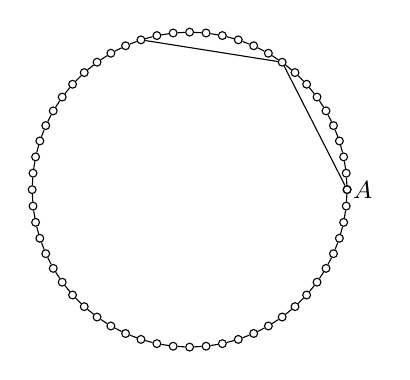
\begin{tikzpicture}[scale=.4]
            \begin{scope}
            \foreach \i in {0,1,2,...,59,60}
            \node[draw,circle,inner sep=1pt]  (v\i) at (6*\i:5) {};
            \foreach \i [remember=\i as \lasti (initially 0)] in {1,2,...,60}
            \draw (v\i) to (v\lasti);
            \draw (v0) to (v9);
            \draw (v9) to (v18);
            \node at (5.5,0) {\small $A$};
            \end{scope}
            \end{tikzpicture}
        \end{QBODY}
        \begin{QFROMS}
        \end{QFROMS}
        \begin{QTAGS}\QTAG{綜合}\end{QTAGS}
        \begin{QANS}
            $20$
        \end{QANS}
        \begin{QSOLLIST}
        \end{QSOLLIST}
        \begin{QEMPTYSPACE}
        \end{QEMPTYSPACE}
    \end{QUESTION}
    \begin{QUESTION}
        \begin{ExamInfo}{091}{學測}{填充}{E}
        \end{ExamInfo}
        \begin{ExamAnsRateInfo}{41}{70}{41}{12}
        \end{ExamAnsRateInfo}
        \begin{QBODY}
            某次網球比賽共有 $128$ 位選手參加,採單淘汰制,每輪淘汰一半的選手,剩下一半的選手進入下一輪。在第 $1$ 輪被淘汰的選手可獲得 $1$ 萬元,在第 $2$ 輪被淘汰的選手可獲得 $2$ 萬元,在第 $k$ 輪被淘汰的選手可獲得 $2^{k-1}$ 萬元,而冠軍則可獲得 $128$ 萬元。試問全部比賽獎金共$\TCNBOX{\TCN\TCN\TCN}$萬元。
        \end{QBODY}
        \begin{QFROMS}
        \end{QFROMS}
        \begin{QTAGS}\QTAG{B2C1數列級數}\end{QTAGS}
        \begin{QANS}
            $576$萬元
        \end{QANS}
        \begin{QSOLLIST}
        \end{QSOLLIST}
        \begin{QEMPTYSPACE}
        \end{QEMPTYSPACE}
    \end{QUESTION}
    \begin{QUESTION}
        \begin{ExamInfo}{091}{學測}{填充}{F}
        \end{ExamInfo}
        \begin{ExamAnsRateInfo}{51}{89}{50}{14}
        \end{ExamAnsRateInfo}
        \begin{QBODY}
            某人隔河測一山高,在 $A$ 點觀測山時,山的方位為東偏北 $60^\circ$,
            山頂的仰角為 $45^\circ$,
            某人自 $A$ 點向東行 $600$ 公尺到達 $B$ 點,山的方位變成在西偏北 $60^\circ$,則山有多高? 答: $
            \TCNBOX{\TCN\TCN\TCN}$ 公尺。
        \end{QBODY}
        \begin{QFROMS}
        \end{QFROMS}
        \begin{QTAGS}\QTAG{B3C1三角}\end{QTAGS}
        \begin{QANS}
            $600$
        \end{QANS}
        \begin{QSOLLIST}
        \end{QSOLLIST}
        \begin{QEMPTYSPACE}
        \end{QEMPTYSPACE}
    \end{QUESTION}
    \begin{QUESTION}
        \begin{ExamInfo}{091}{學測}{填充}{G}
        \end{ExamInfo}
        \begin{ExamAnsRateInfo}{29}{58}{24}{5}
        \end{ExamAnsRateInfo}
        \begin{QBODY}
            有一群體有九位成員,其身高分別為(單位:公分) $160, 163, 166, 170, 172, 174, 176, 178, 180$ , 此九人的平均身高為 $171$ 公分。今隨機抽樣 $3$ 人,則抽到 $3$ 人的平均身高等於母體平均身高的機率為 
            $\TCNBOX{\FR{\TCN}{\TCN\TCN}} $。
        \end{QBODY}
        \begin{QFROMS}
        \end{QFROMS}
        \begin{QTAGS}\QTAG{B2C4數據分析}\end{QTAGS}
        \begin{QANS}
            $\frac{1}{28}$
        \end{QANS}
        \begin{QSOLLIST}
        \end{QSOLLIST}
        \begin{QEMPTYSPACE}
        \end{QEMPTYSPACE}
    \end{QUESTION}
    \begin{QUESTION}
        \begin{ExamInfo}{091}{學測}{填充}{H}
        \end{ExamInfo}
        \begin{ExamAnsRateInfo}{28}{69}{14}{1}
        \end{ExamAnsRateInfo}
        \begin{QBODY}
            右圖為一正立方體,被一平面截出一個四邊形 $ABCD$,
            其中 $B,D$ 分別為稜的中點,
            且 $\overline{EA}: \overline{AF}=1:2$,則 $\cos\angle DAB= $ 
            $\TCNBOX{\FR{\TCN}{\TCN\TCN}}$
            
            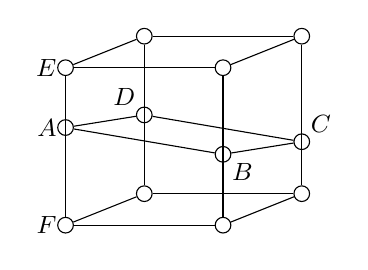
\begin{tikzpicture}
                \small
                \tikzstyle{vnode}=[draw,circle,inner sep =2pt];
                \node[vnode] (v000) at (0,0) {};
                \node[anchor =east] (t000) at (v000) {};
                \node[vnode] (v001) at (0,2) {};
                \node[anchor =east] (t000) at (v001) {};
                \node[vnode] (v011) at (2,2) {};
                \node[anchor =west] (t011) at (v011) {};
                \node[vnode] (v010) at (2,0) {};
                \node[anchor =west] (t010) at (v010) {};
                \node[vnode] (v100) at (-1.0,-.4) {};
                \node[anchor =east] (t100) at (v100) {$F$};
                \node[vnode] (v101) at (-1.0,1.6) {};
                \node[anchor =east] (t101) at (v101) {$E$};
                \node[vnode] (v111) at (1.0,1.6) {};
                \node[anchor =north east] (t111) at (v111) {};
                \node[vnode] (v110) at (1.0,-0.4) {};
                \node[anchor =west] (t110) at (v110) {};
                \node[vnode] (vA) at (-1,.84) {};
                \node[anchor =east] (tA) at (vA) {$A$};
                \node[vnode] (vC) at (2,.66) {};
                \node[anchor =south west] (tC) at (vC) {$C$};
                \node[vnode] (vD) at (0,1) {};
                \node[anchor =south east] (tD) at (vD) {$D$};
                \node[vnode] (vB) at (1,.5) {};
                \node[anchor =north west] (tB) at (vB) {$B$};
                \draw (vD) to[dashed] (vA);
                \draw (vD) to[dashed] (vC);
                \draw (vB) to (vA);
                \draw (vB) to (vC);
                \foreach \i in {01,10,11}{
                    \draw (v0\i) to (v1\i);
                    \draw (v\i  0) to (v\i 1);
                }
                \draw (v000) to[dashed] (v100);
                \draw (v000) to[dashed] (v010);
                \draw (v000) to[dashed] (v001);
                \draw (v001) to (v011);
                \draw (v100) to (v110);
                \draw (v101) to (v111);              
            \end{tikzpicture}
            
        \end{QBODY}
        \begin{QFROMS}
        \end{QFROMS}
        \begin{QTAGS}\QTAG{B4C1空間向量}\end{QTAGS}
        \begin{QANS}
            $\frac{1}{37}$
        \end{QANS}
        \begin{QSOLLIST}
        \end{QSOLLIST}
        \begin{QEMPTYSPACE}
        \end{QEMPTYSPACE}
    \end{QUESTION}
\end{QUESTIONS}

    \begin{QUESTION}
        \begin{ExamInfo}{92}{學測}{單選}{1}
        \end{ExamInfo}
        \begin{ExamAnsRateInfo}{46}{74}{46}{18}
        \end{ExamAnsRateInfo}
        \begin{QBODY}
            試問有多少個正整數 $n$ 使得 $ \dfrac{1}{n} + \dfrac{2}{n} + \cdots + \dfrac{10}{n}$ 為整數? 
            \begin{QOPS} 
                \QOP $1$ 個 
                \QOP $2$ 個  
                \QOP $3$ 個 
                \QOP $4$ 個 
                \QOP $5$ 個
            \end{QOPS}
        \end{QBODY}
        \begin{QFROMS}
        \end{QFROMS}
        \begin{QTAGS}\QTAG{B2C1數列級數}\QTAG{B2C1-2級數}\end{QTAGS}
        \begin{QANS}
            (4)
        \end{QANS}
        \begin{QSOLLIST}
        \end{QSOLLIST}
        \begin{QEMPTYSPACE}
        \end{QEMPTYSPACE}
    \end{QUESTION}
    \begin{QUESTION}
        \begin{ExamInfo}{92}{學測}{單選}{2}
        \end{ExamInfo}
        \begin{ExamAnsRateInfo}{46}{83}{44}{11}
        \end{ExamAnsRateInfo}
        \begin{QBODY}
            若 $f(x)=x^3 - 2x^2 -x +5$,則多項式 $g(x)=f(f(x))$ 除以$(x-2)$ 所得的餘式為 
            \begin{QOPS} 
                \QOP $3 $
                \QOP $5 $
                \QOP $7 $
                \QOP $9 $
                \QOP $11$
            \end{QOPS}
        \end{QBODY}
        \begin{QFROMS}
        \end{QFROMS}
        \begin{QTAGS}\QTAG{B1C2多項式函數}\QTAG{B1C2-2多項式的運算與應用}\QTAG{餘式定理}\end{QTAGS}
        \begin{QANS}
            (5)
        \end{QANS}
        \begin{QSOLLIST}
        \end{QSOLLIST}
        \begin{QEMPTYSPACE}
        \end{QEMPTYSPACE}
    \end{QUESTION}
    \begin{QUESTION}
        \begin{ExamInfo}{92}{學測}{單選}{3}
        \end{ExamInfo}
        \begin{ExamAnsRateInfo}{41}{66}{36}{21}
        \end{ExamAnsRateInfo}
        \begin{QBODY}
            若 $(4 + 3i)(\cos \theta + i \sin \theta )$ 為小於 0 的實數, 則 $\theta$ 是第幾象限角? 
            \begin{QOPS} 
                \QOP 第一象限角 
                \QOP 第二象限角 
                \QOP 第三象限角 
                \QOP 第四象限角 
                \QOP 條件不足,無法判斷
            \end{QOPS}
        \end{QBODY}
        \begin{QFROMS}
        \end{QFROMS}
        \begin{QTAGS}\QTAG{B5C2三角函數II}\end{QTAGS}
        \begin{QANS}
            (2)
        \end{QANS}
        \begin{QSOLLIST}
        \end{QSOLLIST}
        \begin{QEMPTYSPACE}
        \end{QEMPTYSPACE}
    \end{QUESTION}
    \begin{QUESTION}
        \begin{ExamInfo}{92}{學測}{單選}{4}
        \end{ExamInfo}
        \begin{ExamAnsRateInfo}{49}{69}{47}{31}
        \end{ExamAnsRateInfo}
        \begin{QBODY}
            設 $ABC$ 為坐標平面上一三角形,$P$ 為平面上一點且 $\lvec{AP} = \dfrac{1}{5} \lvec{AB} + \dfrac{2}{5} \lvec{AC}$ , 則 $\dfrac{\triangle ABP \mbox{面積}}{ \triangle ABC \mbox{面積}}$等於 
            \begin{QOPS}
                \QOP $\dfrac{1}{5}$ 
                \QOP $\dfrac{1}{4}$ 
                \QOP $\dfrac{2}{5}$ 
                \QOP $\dfrac{1}{2}$         
                \QOP $\dfrac{2}{3}$
            \end{QOPS}
        \end{QBODY}
        \begin{QFROMS}
        \end{QFROMS}
        \begin{QTAGS}\QTAG{面積}\QTAG{B3C3-3面積與二階行列式}\QTAG{B3C3-1平面向量的表示法}\QTAG{B3C3平面向量}\QTAG{線性組合}\end{QTAGS}
        \begin{QANS}
            (3)
        \end{QANS}
        \begin{QSOLLIST}
        \end{QSOLLIST}
        \begin{QEMPTYSPACE}
        \end{QEMPTYSPACE}
    \end{QUESTION}
    \begin{QUESTION}
        \begin{ExamInfo}{92}{學測}{單選}{5}
        \end{ExamInfo}
        \begin{ExamAnsRateInfo}{22}{43}{15}{8}
        \end{ExamAnsRateInfo}
        \begin{QBODY}
            根據統計資料,在  $A$ 小鎮當某件訊息發布後, 
            $t$ 小時之內聽到該訊息的人口是全鎮人口的 $100(1- 2^{-kt})\%$ ,
            其中 $k$ 是某個大於 $0$ 的常數。
            今有某訊息,假設在發布後 $3$ 小時之內已經有 $70\%$ 的人口聽到該訊息。
            又設最快要 $T$ 小時後,有 $99\%$ 的人口已聽到該訊息,則 $T$ 最接近下列哪一個選項?
            \begin{QOPS} 
                \QOP $5$小時        
                \QOP $7\frac{1}{2}$小時
                \QOP $9$小時 
                \QOP $11\frac{1}{2}$小時 
                \QOP $13$小時
            \end{QOPS}
        \end{QBODY}
        \begin{QFROMS}
        \end{QFROMS}
        \begin{QTAGS}\QTAG{應用問題}\QTAG{B1C3指對數函數}\QTAG{B1C3-5指數與對數的應用}\end{QTAGS}
        \begin{QANS}
            (4)
        \end{QANS}
        \begin{QSOLLIST}
        \end{QSOLLIST}
        \begin{QEMPTYSPACE}
        \end{QEMPTYSPACE}
    \end{QUESTION}
    \begin{QUESTION}
        \begin{ExamInfo}{92}{學測}{多選}{6}
        \end{ExamInfo}
        \begin{ExamAnsRateInfo}{41}{71}{40}{12}
        \end{ExamAnsRateInfo}
        \begin{QBODY}
            如右圖,兩直線 $L_1$ 、 $L_2$ 之方程式分別為 $L_1 : x+ay+b=0$, $L_2 :x+cy+d=0$;試問下列哪些選項是正確的? 
            \begin{QOPS} 
                \QOP $a>0$ 
                \QOP $b>0$ 
                \QOP $c>0$ 
                \QOP $d>0$ 
                \QOP $a<c$ 
            \end{QOPS}
            
            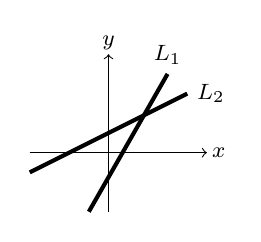
\begin{tikzpicture}[scale=.5]\footnotesize
            \begin{scope}
            \pgfsetarrowsend{latex}
            \draw[->]  (-2,0) to(2.5,0);
            \draw[->] (0,-1.5) to (0,2.5);
            \end{scope}
            \pgfsetlinewidth{1.5pt}
            \node at (0,2.8) {$y$};
            \node at (2.8,0) {$x$};
            \draw (-2,-0.5) to (2,1.5) node[right] {$L_2$};
            \draw (-.5,-1.5) to (1.5,2)node[above] {$L_1$} ;
            \end{tikzpicture}
        \end{QBODY}
        \begin{QFROMS}
        \end{QFROMS}
        \begin{QTAGS}\QTAG{B3C2-1直線方程式及其圖形}\QTAG{圖形}\QTAG{B3C2直線與圓}\end{QTAGS}
        \begin{QANS}
            (4)(5)
        \end{QANS}
        \begin{QSOLLIST}
        \end{QSOLLIST}
        \begin{QEMPTYSPACE}
        \end{QEMPTYSPACE}
    \end{QUESTION}
    \begin{QUESTION}
        \begin{ExamInfo}{92}{學測}{多選}{7}
        \end{ExamInfo}
        \begin{ExamAnsRateInfo}{45}{79}{41}{15}
        \end{ExamAnsRateInfo}
        \begin{QBODY}
            如右圖,$ABCD-EFGH$ 為一平行六面體,$J$ 為四邊形 $BCGF$ 的中心,
            如果 $\lvec{AJ} = a \lvec{AB} + b\lvec{AD}+ c\lvec{AE}$,
            試問下列哪些選項是正確的? 
            \begin{QOPS} 
                \QOP $\frac{1}{3} < b < \frac{2}{3}$ 
                \QOP $a + b + c = 2$  
                \QOP $a=1$
                \QOP $a=2c$ 
                \QOP $a=b$
            \end{QOPS}
        
            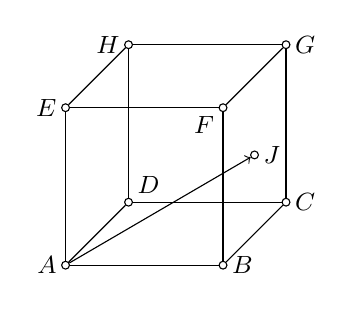
\begin{tikzpicture}
                \begin{scope}
                \small
                \tikzstyle{vnode}=[draw,circle,inner sep =1pt];
                \node[vnode] (v000) at (0,0) {};
                \node[anchor =south west] (t000) at (v000) {$D$};
                \node[vnode] (v001) at (0,2) {$$};
                \node[anchor =east] (t000) at (v001) {$H$};
                \node[vnode] (v011) at (2,2) {$$};
                \node[anchor =west] (t011) at (v011) {$G$};
                \node[vnode] (v010) at (2,0) {$$};
                \node[anchor =west] (t010) at (v010) {$C$};
                \node[vnode] (v100) at (-.8,-.8) {$$};
                \node[anchor =east] (t100) at (v100) {$A$};
                \node[vnode] (v101) at (-.8,1.2) {$$};
                \node[anchor =east] (t101) at (v101) {$E$};
                \node[vnode] (v111) at (1.2,1.2) {$$};
                \node[anchor =north east] (t111) at (v111) {$F$};
                \node[vnode] (v110) at (1.2,-0.8) {$$};
                \node[anchor =west] (t110) at (v110) {$B$};
                \node[vnode] (vJ) at (1.6, .6) {$$};
                \node[anchor =west] (tJ) at (vJ) {$J$};
                \foreach \i in {01,10,11}{
                    \draw (v0\i) to (v1\i);
                    \draw (v\i  0) to (v\i 1);
                }
                \draw (v000) to[dashed] (v100);
                \draw (v000) to[dashed] (v010);
                \draw (v000) to[dashed] (v001);
                \draw (v001) to (v011);
                \draw (v100) to (v110);
                \draw (v101) to (v111);
                \draw[->] (v100) to (vJ);
                \end{scope}
            \end{tikzpicture}
        \end{QBODY}
        \begin{QFROMS}
        \end{QFROMS}
        \begin{QTAGS}\QTAG{B4C1-2空間向量的坐標表示法}\QTAG{B4C1空間向量}\end{QTAGS}
        \begin{QANS}
            (1)(2)(3)(4)
        \end{QANS}
        \begin{QSOLLIST}
        \end{QSOLLIST}
        \begin{QEMPTYSPACE}
        \end{QEMPTYSPACE}
    \end{QUESTION}
    \begin{QUESTION}
        \begin{ExamInfo}{92}{學測}{多選}{8}
        \end{ExamInfo}
        \begin{ExamAnsRateInfo}{55}{86}{60}{19}
        \end{ExamAnsRateInfo}
        \begin{QBODY}
            以下各數何者為正? 
            \begin{QOPS} 
                \QOP $\sqrt{2} - \sqrt[3]{2}$ 
                \QOP $\log_{2} 3-1$ 
                \QOP $\log_{3}2 -1$ 
                \QOP $\log_{\frac{1}{2}} 3$ 
                \QOP $\log_{\frac{1}{3}} \frac{1}{2}$ 
            \end{QOPS}
        \end{QBODY}
        \begin{QFROMS}
        \end{QFROMS}
        \begin{QTAGS}\QTAG{B1C3-2指數函數}\QTAG{B1C3指對數函數}\QTAG{指數律}\end{QTAGS}
        \begin{QANS}
            (1)(2)(5)
        \end{QANS}
        \begin{QSOLLIST}
        \end{QSOLLIST}
        \begin{QEMPTYSPACE}
        \end{QEMPTYSPACE}
    \end{QUESTION}
    \begin{QUESTION}
        \begin{ExamInfo}{92}{學測}{多選}{9}
        \end{ExamInfo}
        \begin{ExamAnsRateInfo}{24}{42}{19}{11}
        \end{ExamAnsRateInfo}
        \begin{QBODY}
            下列哪些函數的最小正週期為 $\pi$ ? 
            \begin{QOPS} 
                \QOP $\sin x + \cos x$ 
                \QOP $\sin x - \cos x$ 
                \QOP $|\sin x + \cos x|$
                \QOP $|\sin x - \cos x|$ 
                \QOP $|\sin x| + |\cos x|$
            \end{QOPS}
        \end{QBODY}
        \begin{QFROMS}
        \end{QFROMS}
        \begin{QTAGS}\QTAG{B5C2-1一般三角函數的性質與圖形}\QTAG{B5C2三角函數II}\end{QTAGS}
        \begin{QANS}
            (3)(4)
        \end{QANS}
        \begin{QSOLLIST}
        \end{QSOLLIST}
        \begin{QEMPTYSPACE}
        \end{QEMPTYSPACE}
    \end{QUESTION}
    \begin{QUESTION}
        \begin{ExamInfo}{92}{學測}{多選}{10}
        \end{ExamInfo}
        \begin{ExamAnsRateInfo}{21}{43}{14}{6}
        \end{ExamAnsRateInfo}
        \begin{QBODY}
            假設坐標平面上一非空集合 $S$ 試問下列哪些敘述對 $S$ 內的點 $(x, y)$ 具有以下性質:「若  $x > 0$,則 $y > 0$」。 試問下列哪些敘述對 $S$ 內的點 $(x, y)$ 必定成立? 
            \begin{QOPS} 
                \QOP 若 $x \leq 0$,則 $y \leq 0$ ;
                \QOP 若 $y \leq 0$, 則 $x \leq 0$;
                \QOP 若 $y \leq 0$,則 $x \leq 0$ ; 
                \QOP 若 $x >1$,則 $y>0$;  \QOP 若 $y<0$ ,則 $x \leq 0$。
            \end{QOPS}
        \end{QBODY}
        \begin{QFROMS}
        \end{QFROMS}
        \begin{QTAGS}\QTAG{不是99課綱}\end{QTAGS}
        \begin{QANS}
            (2)(4)(5)
        \end{QANS}
        \begin{QSOLLIST}
        \end{QSOLLIST}
        \begin{QEMPTYSPACE}
        \end{QEMPTYSPACE}
    \end{QUESTION}
    \begin{QUESTION}
        \begin{ExamInfo}{92}{學測}{多選}{11}
        \end{ExamInfo}
        \begin{ExamAnsRateInfo}{24}{43}{18}{11}
        \end{ExamAnsRateInfo}
        \begin{QBODY}
            設 $\pi_a : x-4y +az=10$ ($a$為常數), $E_1 :x-2y+z=5$ 及 $E_2  :2x-5y+4z=3$ 為坐標空間中的三個平面。
            試問下列哪些敘述是正確的?
            
            \begin{QOPS} 
                \QOP 存在實數 $a$ 使得 $\pi_a$ 與 $E_1$ 平行;
                \QOP 存在實數 $a$ 使得 $\pi_a$ 與 $E_1$ 垂直;
                \QOP 存在實數 $a$ 使得 $\pi_a$ , $E_1$, $E_2$ 交於一點; 
                \QOP 存在實數 $a$ 使得 $\pi_a, E_1, E_2 $ 交於一直線;
                \QOP 存在實數 $a$ 使得 $\pi_a$, $E_1$ , $E_2$ 沒有共同交點。\end{QOPS}
        \end{QBODY}
        \begin{QFROMS}
        \end{QFROMS}
        \begin{QTAGS}\QTAG{B4C3矩陣}\QTAG{B4C3-1線性方程組與矩陣}\QTAG{方程組}\end{QTAGS}
        \begin{QANS}
            (2)(3)(5)
        \end{QANS}
        \begin{QSOLLIST}
        \end{QSOLLIST}
        \begin{QEMPTYSPACE}
        \end{QEMPTYSPACE}
    \end{QUESTION}
    \begin{QUESTION}
        \begin{ExamInfo}{92}{學測}{填充}{A}
        \end{ExamInfo}
        \begin{ExamAnsRateInfo}{37}{74}{31}{6}
        \end{ExamAnsRateInfo}
        \begin{QBODY}
            設 $a_1,a_2,\cdots,a_{50}$ 是從 $-1,0,1$ 這三個整數中取值的數列。若 $a_1 +a_2 + \cdots + a_{50} = 9$ 且 $(a_1+1)^2 +(a_2 +1)^2 + \cdots + (a_{50} +1)^2 =107$, 則 $a_1,a_2,\cdots,a_{50}$ 當中有幾項是 $0$?答: 
            $\TCNBOX{\TCN\TCN}$ 項。
        \end{QBODY}
        \begin{QFROMS}
        \end{QFROMS}
        \begin{QTAGS}\QTAG{B2C1數列級數}\QTAG{特殊數列}\QTAG{B2C1-2級數}\QTAG{B2C1-1數列}\end{QTAGS}
        \begin{QANS}
            $11$
        \end{QANS}
        \begin{QSOLLIST}
        \end{QSOLLIST}
        \begin{QEMPTYSPACE}
        \end{QEMPTYSPACE}
    \end{QUESTION}
    \begin{QUESTION}
        \begin{ExamInfo}{92}{學測}{填充}{B}
        \end{ExamInfo}
        \begin{ExamAnsRateInfo}{64}{93}{70}{29}
        \end{ExamAnsRateInfo}
        \begin{QBODY}
            金先生在提款時忘了帳號密碼,但他還記得密碼的四位數字中,有兩個 $3$, 一個 $8$,一個 $9$,於是他就用這四個數字隨意排成一個四位數輸入提款機嘗試。請問他只試一次就成功的機率有多少? $\TCNBOX{\FR{\TCN}{\TCN\TCN}}$
        \end{QBODY}
        \begin{QFROMS}
        \end{QFROMS}
        \begin{QTAGS}\QTAG{B2C3機率}\QTAG{B2C3-2機率的定義與性質}\end{QTAGS}
        \begin{QANS}
            $\frac{1}{12}$
        \end{QANS}
        \begin{QSOLLIST}
        \end{QSOLLIST}
        \begin{QEMPTYSPACE}
        \end{QEMPTYSPACE}
    \end{QUESTION}
    \begin{QUESTION}
        \begin{ExamInfo}{92}{學測}{填充}{C}
        \end{ExamInfo}
        \begin{ExamAnsRateInfo}{27}{52}{21}{8}
        \end{ExamAnsRateInfo}
        \begin{QBODY}
            設 $A(1,0)$ 與 $B(b,0)$ 為坐標平面上的兩點, 其中 $b>1$。 
            若拋物線 $\Gamma : y^2=4x$ 上有一點 $P$ 使得 $\triangle ABP$ 為一正三角形,則 $b= 
            \TCNBOX{\TCN}$。
        \end{QBODY}
        \begin{QFROMS}
        \end{QFROMS}
        \begin{QTAGS}\QTAG{B4C4二次曲線}\QTAG{B4C4-1拋物線}\QTAG{圖形}\end{QTAGS}
        \begin{QANS}
            $5$
        \end{QANS}
        \begin{QSOLLIST}
        \end{QSOLLIST}
        \begin{QEMPTYSPACE}
        \end{QEMPTYSPACE}
    \end{QUESTION}
    \begin{QUESTION}
        \begin{ExamInfo}{92}{學測}{填充}{D}
        \end{ExamInfo}
        \begin{ExamAnsRateInfo}{16}{39}{7}{2}
        \end{ExamAnsRateInfo}
        \begin{QBODY}
            設 $P$ 為雙曲線 $\dfrac{x^2}{9} - \dfrac{y^2}{16} = 1$ 上的一點且位在第一象限。若 $F_1$,  $F_2$ 為此雙曲線的兩個焦點,且 $\overline{PF}_1 : \overline{PF}_2 = 1:3 $,則 $\triangle F_1PF_2$ 的周長等於 $
            \TCNBOX{\TCN\TCN}$。
        \end{QBODY}
        \begin{QFROMS}
        \end{QFROMS}
        \begin{QTAGS}\QTAG{B4C4-3雙曲線}\QTAG{B4C4二次曲線}\QTAG{圖形}\end{QTAGS}
        \begin{QANS}
            $22$
        \end{QANS}
        \begin{QSOLLIST}
        \end{QSOLLIST}
        \begin{QEMPTYSPACE}
        \end{QEMPTYSPACE}
    \end{QUESTION}
    \begin{QUESTION}
        \begin{ExamInfo}{92}{學測}{填充}{E}
        \end{ExamInfo}
        \begin{ExamAnsRateInfo}{21}{37}{17}{9}
        \end{ExamAnsRateInfo}
        \begin{QBODY}
            在坐標空間中,通過 $O(0,0,0)$, $N(0,0,1)$, $P(\dfrac{1}{4}, \dfrac{\sqrt{11}}{4}, -\dfrac{1}{2})$ 三點的平面與球面  $S: x^2+y^2+z^2=1$相交於一個圓 $C$,則圓 $C$ 的劣弧 $NP$ 的弧長等於 
            $\TCNBOX{\FR{\TCN}{\TCN} \pi} $。
        \end{QBODY}
        \begin{QFROMS}
        \end{QFROMS}
        \begin{QTAGS}\QTAG{不是99課綱}\end{QTAGS}
        \begin{QANS}
            $\frac{2}{3}\pi$
        \end{QANS}
        \begin{QSOLLIST}
        \end{QSOLLIST}
        \begin{QEMPTYSPACE}
        \end{QEMPTYSPACE}
    \end{QUESTION}
    \begin{QUESTION}
        \begin{ExamInfo}{92}{學測}{填充}{F}
        \end{ExamInfo}
        \begin{ExamAnsRateInfo}{35}{67}{31}{7}
        \end{ExamAnsRateInfo}
        \begin{QBODY}
            設 $k$ 為一整數,若方程式 $kx^2 + 7x +1= 0$ 有兩個相異實根,且兩根的乘積介於 $\dfrac{5}{71}$ 與 $\dfrac{6}{71}$之間,則 $k=\TCNBOX{\TCN\TCN}$。
        \end{QBODY}
        \begin{QFROMS}
        \end{QFROMS}
        \begin{QTAGS}\QTAG{B1C2-3多項式方程式}\QTAG{根與係數的關係}\QTAG{B1C2多項式函數}\QTAG{韋達定理}\end{QTAGS}
        \begin{QANS}
            $12$
        \end{QANS}
        \begin{QSOLLIST}
        \end{QSOLLIST}
        \begin{QEMPTYSPACE}
        \end{QEMPTYSPACE}
    \end{QUESTION}
    \begin{QUESTION}
        \begin{ExamInfo}{92}{學測}{填充}{G}
        \end{ExamInfo}
        \begin{ExamAnsRateInfo}{15}{41}{4}{0}
        \end{ExamAnsRateInfo}
        \begin{QBODY}
            在只有皮尺沒有梯子的情形下,想要測出一拋物線形拱門的高度。
            已知此拋物線以過最高點的鉛垂線為對稱軸。
            現甲、乙兩人以皮尺測得拱門底部寬為 $6$ 公尺,且距底部 $\frac{3}{2}$ 公尺高處其寬為 $5$ 公尺。
            利用這些數據可推算出拱門的高度為$\TCNBOX{\FR{\TCN\TCN}{\TCN\TCN}}$ 公尺。
        \end{QBODY}
        \begin{QFROMS}
        \end{QFROMS}
        \begin{QTAGS}\QTAG{B1C2多項式函數}\QTAG{圖形}\QTAG{二次多項式}\QTAG{B1C2-1簡單的多項式及圖形}\QTAG{最值}\end{QTAGS}
        \begin{QANS}
            $\dfrac{54}{11}$
        \end{QANS}
        \begin{QSOLLIST}
        \end{QSOLLIST}
        \begin{QEMPTYSPACE}
        \end{QEMPTYSPACE}
    \end{QUESTION}
    \begin{QUESTION}
        \begin{ExamInfo}{92}{學測}{填充}{H}
        \end{ExamInfo}
        \begin{ExamAnsRateInfo}{17}{36}{12}{3}
        \end{ExamAnsRateInfo}
        \begin{QBODY}
            某次數學測驗共有 $25$ 題單一選擇題,每題都有五個選項,每答對一題可得 $4$ 分,答錯倒扣 $1$ 分。某生確定其中 $16$ 題可答對;有 $6$ 題他確定五個選項中有兩個選項不正確,因此這 $6$ 題他就從剩下的選項中分別猜選一個;另外 $3$ 題只好亂猜,則他這次測驗得分之期望值為 
            \TCNBOX{\TCN\TCN} 分。(計算到整數為止,小數點以後四捨五入。)
        \end{QBODY}
        \begin{QFROMS}
        \end{QFROMS}
        \begin{QTAGS}\QTAG{B5C1機率與統計}\end{QTAGS}
        \begin{QANS}
            $68$
        \end{QANS}
        \begin{QSOLLIST}
        \end{QSOLLIST}
        \begin{QEMPTYSPACE}
        \end{QEMPTYSPACE}
    \end{QUESTION}
    \begin{QUESTION}
        \begin{ExamInfo}{92}{學測}{填充}{I}
        \end{ExamInfo}
        \begin{ExamAnsRateInfo}{38}{70}{35}{9}
        \end{ExamAnsRateInfo}
        \begin{QBODY}
            根據統計資料,$1$ 月份台北地區的平均氣溫是攝氏 $16$ 度,
            標準差是攝氏 $3.5$ 度。一般外國朋友比較習慣用華氏溫度來表示冷熱,
            已知當攝氏溫度為 $x$ 時,華氏溫度為 $y =\dfrac{9}{5}x + 32$;
            若用華氏溫度表示,則 1 月份台北地區的平均氣溫是華氏 
            \TCNBOX{\TCN\TCN.\TCN} 度,
            標準差是華氏 
            \TCNBOX{\TCN.\TCN} 度。(計算到小數點後第一位,以下四捨五入。)
        \end{QBODY}
        \begin{QFROMS}
        \end{QFROMS}
        \begin{QTAGS}\QTAG{平均數}\QTAG{B2C4-1一維數據分析}\QTAG{B2C4數據分析}\QTAG{線性公式}\QTAG{標準差}\end{QTAGS}
        \begin{QANS}
            $60.8$, $6.3$
        \end{QANS}
        \begin{QSOLLIST}
        \end{QSOLLIST}
        \begin{QEMPTYSPACE}
        \end{QEMPTYSPACE}
    \end{QUESTION}

    \begin{QUESTION}
        \begin{ExamInfo}{93}{學測}{單選}{1}
        \end{ExamInfo}
        \begin{ExamAnsRateInfo}{71}{93}{79}{41}
        \end{ExamAnsRateInfo}
        \begin{QBODY}
            已知一等差數列共有十項,且知其奇數項之和為15,偶數項之和為30,則下列哪一選項為此數列之公差? 
            \begin{QOPS} 
                \QOP 1 
                \QOP 2 
                \QOP 3 
                \QOP 4 
                \QOP 5 
            \end{QOPS}
        \end{QBODY}
        \begin{QFROMS}
        \end{QFROMS}
        \begin{QTAGS}\QTAG{B2C1數列級數}\QTAG{等差級數}\QTAG{B2C1-2級數}\QTAG{B2C1-1數列}\QTAG{等差數列}\end{QTAGS}
        \begin{QANS}
            (3)
        \end{QANS}
        \begin{QSOLLIST}
        \end{QSOLLIST}
        \begin{QEMPTYSPACE}
        \end{QEMPTYSPACE}
    \end{QUESTION}
    \begin{QUESTION}
        \begin{ExamInfo}{93}{學測}{單選}{2}
        \end{ExamInfo}
        \begin{ExamAnsRateInfo}{60}{85}{62}{33}
        \end{ExamAnsRateInfo}
        \begin{QBODY}
            下列選項中的數,何者最大? 
            \begin{QOPS} 
                \QOP $100^{10}$ 
                \QOP $10^{100}$ 
                \QOP $50^{50} $
                \QOP $50!$ 
                \QOP $\frac{100!}{50!}$。 
            \end{QOPS}
        \end{QBODY}
        \begin{QFROMS}
        \end{QFROMS}
        \begin{QTAGS}\QTAG{B1C3-1指數}\QTAG{B1C3指對數函數}\end{QTAGS}
        \begin{QANS}
            (2)
        \end{QANS}
        \begin{QSOLLIST}
        \end{QSOLLIST}
        \begin{QEMPTYSPACE}
        \end{QEMPTYSPACE}
    \end{QUESTION}
    \begin{QUESTION}
        \begin{ExamInfo}{93}{學測}{單選}{3}
        \end{ExamInfo}
        \begin{ExamAnsRateInfo}{44}{76}{40}{16}
        \end{ExamAnsRateInfo}
        \begin{QBODY}
            右圖陰影部分所示為複數平面上區域 $A= \{ z:z=r(\cos \theta +i\sin \theta), 0\leq r \leq 1, \frac{3}{4} \pi \leq \theta \leq \frac{5}{4} \pi \} $ 之略圖。
            令 $D =\{ w:w = z^3 , z \in A\}$,試問下列選項中之略圖,何者之陰影部分與區域 $D$ 最接近?
            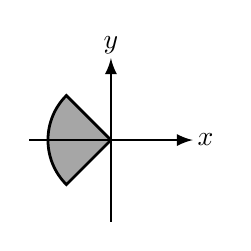
\begin{tikzpicture}[scale=.8]
            \begin{scope}
            \pgfsetlinewidth{1pt}
            \draw[fill=gray!70] (0,0) -- (135:1cm) arc (135:225:1cm) -- (0,0);
            \node at (0,1.5) {$y$};
            \node at (1.5,0) {$x$};
            \pgfsetarrowsend{latex}
            \draw (-1.3,0) to[->] (1.3,0);
            \draw (0,-1.3) to[->] (0,1.3);
            \end{scope}
            \end{tikzpicture}
            \begin{QOPS}
                \QOP 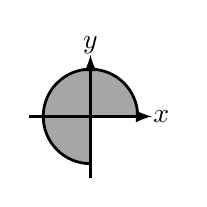
\begin{tikzpicture}[scale=.6]
                    \begin{scope}
                    \pgfsetlinewidth{1pt}
                    \draw[fill=gray!70] (0,0) -- (0:1cm) arc (0:270:1cm) -- (0,0);
                    \node at (0,1.5) {$y$};
                    \node at (1.5,0) {$x$};
                    \pgfsetarrowsend{latex}
                    \draw (-1.3,0) to[->] (1.3,0);
                    \draw (0,-1.3) to[->] (0,1.3);
                    \end{scope}
                    \end{tikzpicture}
                
                \QOP 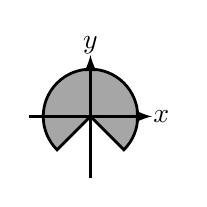
\begin{tikzpicture}[scale=.6]
                    \begin{scope}
                    \pgfsetlinewidth{1pt}
                    \draw[fill=gray!70] (0,0) -- (-45:1cm) arc (-45:225:1cm) -- (0,0);
                    \node at (0,1.5) {$y$};
                    \node at (1.5,0) {$x$};
                    \pgfsetarrowsend{latex}
                    \draw (-1.3,0) to[->] (1.3,0);
                    \draw (0,-1.3) to[->] (0,1.3);
                    \end{scope}
                    \end{tikzpicture}
                    
                \QOP 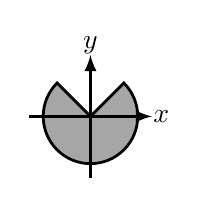
\begin{tikzpicture}[scale=.6]
                    \begin{scope}
                    \pgfsetlinewidth{1pt}
                    \draw[fill=gray!70] (0,0) -- (135:1cm) arc (-225:45:1cm) -- (0,0);
                    \node at (0,1.5) {$y$};
                    \node at (1.5,0) {$x$};
                    \pgfsetarrowsend{latex}
                    \draw (-1.3,0) to[->] (1.3,0);
                    \draw (0,-1.3) to[->] (0,1.3);
                    \end{scope}
                    \end{tikzpicture}
                \QOP 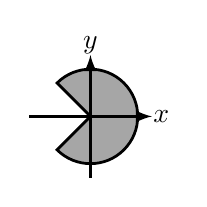
\begin{tikzpicture}[scale=.6]
                \begin{scope}
                \pgfsetlinewidth{1pt}
                \draw[fill=gray!70] (0,0) -- (225:1cm) arc (-135:135:1cm) -- (0,0);
                \node at (0,1.5) {$y$};
                \node at (1.5,0) {$x$};
                \pgfsetarrowsend{latex}
                \draw (-1.3,0) to[->] (1.3,0);
                \draw (0,-1.3) to[->] (0,1.3);
                \end{scope}
                \end{tikzpicture}
                
                \QOP 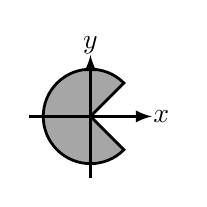
\begin{tikzpicture}[scale=.6]
                    \begin{scope}
                    \pgfsetlinewidth{1pt}
                    \draw[fill=gray!70] (0,0) -- (45:1cm) arc (45:315:1cm) -- (0,0);
                    \node at (0,1.5) {$y$};
                    \node at (1.5,0) {$x$};
                    \pgfsetarrowsend{latex}
                    \draw (-1.3,0) to[->] (1.3,0);
                    \draw (0,-1.3) to[->] (0,1.3);
                    \end{scope}
                    \end{tikzpicture}
            \end{QOPS}
        \end{QBODY}
        \begin{QFROMS}
        \end{QFROMS}
        \begin{QTAGS}\QTAG{B5C2三角函數II}\end{QTAGS}
        \begin{QANS}
            (5)
        \end{QANS}
        \begin{QSOLLIST}
        \end{QSOLLIST}
        \begin{QEMPTYSPACE}
        \end{QEMPTYSPACE}
    \end{QUESTION}
    \begin{QUESTION}
        \begin{ExamInfo}{93}{學測}{單選}{4}
        \end{ExamInfo}
        \begin{ExamAnsRateInfo}{23}{42}{17}{10}
        \end{ExamAnsRateInfo}
        \begin{QBODY}
            在坐標空間中給定兩點 $A(1,2,3)$ 與 $B(7,6,5)$。令 $S$ 為 $xy$- 平面上所有使得向量 $PA$ 垂直於向量 $PB$ 的 $P$ 點所成的集合,則
            \begin{QOPS} 
                \QOP $S$ 為空集合 
                \QOP $S$ 恰含一點 
                \QOP $S$ 恰含兩點 
                \QOP $S$ 為一線段 
                \QOP $S$ 為一圓
            \end{QOPS}
        \end{QBODY}
        \begin{QFROMS}
        \end{QFROMS}
        \begin{QTAGS}\QTAG{B4C1空間向量}\end{QTAGS}
        \begin{QANS}
            (1)
        \end{QANS}
        \begin{QSOLLIST}
        \end{QSOLLIST}
        \begin{QEMPTYSPACE}
        \end{QEMPTYSPACE}
    \end{QUESTION}
    \begin{QUESTION}
        \begin{ExamInfo}{93}{學測}{單選}{5}
        \end{ExamInfo}
        \begin{ExamAnsRateInfo}{61}{88}{62}{33}
        \end{ExamAnsRateInfo}
        \begin{QBODY}
            設 $\triangle ABC$ 為平面上的一個三角形,$P$ 為平面上一點且 $\lvec{AP}= \frac{1}{3}\lvec{AB}+ t\lvec{AC}$,其中 $t$為一實數。
            試問下列哪一選項為 $t$ 的最大範圍,使得 $P$ 落在 $\triangle ABC$ 的內部? 
            \begin{QOPS} 
                \QOP $0<t < \frac{1}{4}$ 
                \QOP $0 < t < \frac{1}{3}$ 
                \QOP $0 < t <\frac{1}{2}$ 
                \QOP $0 < t < \frac{2}{3}$ 
                \QOP $0 < t < \frac{3}{4}$
            \end{QOPS}
        \end{QBODY}
        \begin{QFROMS}
        \end{QFROMS}
        \begin{QTAGS}\QTAG{線性組合}\QTAG{B3C3-1平面向量的表示法}\QTAG{B3C3平面向量}\end{QTAGS}
        \begin{QANS}
            (4)
        \end{QANS}
        \begin{QSOLLIST}
        \end{QSOLLIST}
        \begin{QEMPTYSPACE}
        \end{QEMPTYSPACE}
    \end{QUESTION}
    \begin{QUESTION}
        \begin{ExamInfo}{93}{學測}{單選}{6}
        \end{ExamInfo}
        \begin{ExamAnsRateInfo}{26}{42}{27}{9}
        \end{ExamAnsRateInfo}
        \begin{QBODY}
            台灣證劵交易市場規定股票成交價格只能在前一個交易日的收盤價的漲、跌 $7\%$ 範圍內變動。例如:某支股票前一個交易日的收盤價是每股 100 元,則今天該支股票每股的買賣價格必須在 93 元至 107 元之間。假設有某支股票的價格起伏很大,某一天的收盤價是每股 40 元,次日起連續五個交易日以跌停板收盤 (每天跌 $7\%$),緊接著卻連續五個交易日以漲停板收盤(每天漲 $7\%$)。請問經過這十個交易日後,該支股票每股的收盤價最接近下列哪一個選項中的價格?
            \begin{QOPS}
                \QOP $39$ 元
                \QOP $39.5$ 元
                \QOP $40$ 元
                \QOP $40.5$ 元
                \QOP $41$ 元
            \end{QOPS}
        \end{QBODY}
        \begin{QFROMS}
        \end{QFROMS}
        \begin{QTAGS}\QTAG{應用問題}\QTAG{B1C3指對數函數}\QTAG{B1C3-5指數與對數的應用}\end{QTAGS}
        \begin{QANS}
            (1)
        \end{QANS}
        \begin{QSOLLIST}
        \end{QSOLLIST}
        \begin{QEMPTYSPACE}
        \end{QEMPTYSPACE}
    \end{QUESTION}
    \begin{QUESTION}
        \begin{ExamInfo}{93}{學測}{多選}{7}
        \end{ExamInfo}
        \begin{ExamAnsRateInfo}{56}{77}{61}{30}
        \end{ExamAnsRateInfo}
        \begin{QBODY}
            中山高速公路重慶北路交流道南下入口匝道分成內、外兩線車道,路旁立有標誌 「外側車道 大客車專用」。請選出不違反此規定的選項:
            \begin{QOPS}
                \QOP 小型車行駛內側車道 
                \QOP 小型車行駛外側車道 
                \QOP 大客車行駛內側車道 
                \QOP 大客車行駛外側車道 
                \QOP 大貨車行駛外側車道
            \end{QOPS}
        \end{QBODY}
        \begin{QFROMS}
        \end{QFROMS}
        \begin{QTAGS}\QTAG{邏輯}\QTAG{B2C2-1簡單的邏輯與集合}\QTAG{B2C2排列組合}\end{QTAGS}
        \begin{QANS}
            (1)(3)(4)
        \end{QANS}
        \begin{QSOLLIST}
        \end{QSOLLIST}
        \begin{QEMPTYSPACE}
        \end{QEMPTYSPACE}
    \end{QUESTION}
    \begin{QUESTION}
        \begin{ExamInfo}{93}{學測}{多選}{8}
        \end{ExamInfo}
        \begin{ExamAnsRateInfo}{43}{77}{39}{13}
        \end{ExamAnsRateInfo}
        \begin{QBODY}
            在坐標平面上,下列哪些方程式的圖形可以放進一個夠大的圓裡面? 
            \begin{QOPS} 
                \QOP $3x=2y^2$ 
                \QOP $3x^2+2y^2=1$ 
                \QOP $3x^2-2y^2=1$ \QOP $|x+y|=1$ 
                \QOP $|x|+|y|=1$
            \end{QOPS}
        \end{QBODY}
        \begin{QFROMS}
        \end{QFROMS}
        \begin{QTAGS}\QTAG{跨章節試題}\end{QTAGS}
        \begin{QANS}
            (2)(5)
        \end{QANS}
        \begin{QSOLLIST}
        \end{QSOLLIST}
        \begin{QEMPTYSPACE}
        \end{QEMPTYSPACE}
    \end{QUESTION}
    \begin{QUESTION}
        \begin{ExamInfo}{93}{學測}{多選}{9}
        \end{ExamInfo}
        \begin{ExamAnsRateInfo}{46}{70}{38}{30}
        \end{ExamAnsRateInfo}
        \begin{QBODY}
            如右圖 $O-ABCD$ 為一金字塔,底是邊長為 $1$ 之正方形,
            頂點 $O$ 與 $A$, $B$, $C$, $D$ 之距離均為 2。試問下列哪些式子是正確的?
            \begin{QOPS} 
                \QOP  $\lvec{OA}+\lvec{OB} +\lvec{OC}+\lvec{OD}=\lvec{0}$, 
                \QOP $\lvec{OA} + \lvec{OB}$  $-\lvec{OC}- \lvec{OD} =\lvec{0}$ 
                \QOP $\lvec{OA}- \lvec{OB}+ \lvec{OC} -\lvec{OD}= \lvec{0}$ 
                \QOP $\lvec{OA} \cdot \lvec{OB} = \lvec{OC} \cdot \lvec{OD}$
                \QOP $\lvec{OA}\cdot \lvec{OC}=2$。
            \end{QOPS}
            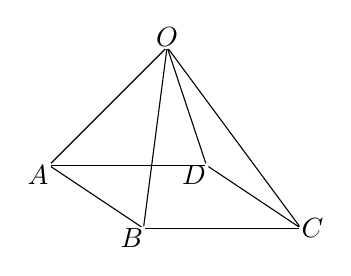
\begin{tikzpicture}[inner sep=0pt]
            \node (v00) at (0,0) {};
            \node[anchor =north east] (t00) at (v00) {$A$};
            \node (v01) at (1.2,-.8) {};
            \node[anchor =north east] (t01) at (v01) {$B$};
            \node (v10) at (2,0) {};
            \node[anchor = north east] (t10) at (v10) {$D$};
            \node (v11) at (3.2,-.8) {};
            \node[anchor =west] (t11) at (v11) {$C$};
            \node (vtop) at (1.5,1.5) {};
            \node[anchor =south] (ttop) at (vtop) {$O$};
            \draw (v00) to (v01);
            \draw (v00) to (v10);
            \draw (v11) to (v01);
            \draw (v11) to (v10);
            \draw (vtop) to (v01);
            \draw (vtop) to (v10);
            \draw (vtop) to (v11);
            \draw (vtop) to (v00);
            \end{tikzpicture}
        \end{QBODY}
        \begin{QFROMS}
        \end{QFROMS}
        \begin{QTAGS}\QTAG{B4C1-2空間向量的坐標表示法}\QTAG{B4C1空間向量}\end{QTAGS}
        \begin{QANS}
            (3)(4)
        \end{QANS}
        \begin{QSOLLIST}
        \end{QSOLLIST}
        \begin{QEMPTYSPACE}
        \end{QEMPTYSPACE}
    \end{QUESTION}
    \begin{QUESTION}
        \begin{ExamInfo}{93}{學測}{多選}{10}
        \end{ExamInfo}
        \begin{ExamAnsRateInfo}{43}{77}{40}{12}
        \end{ExamAnsRateInfo}
        \begin{QBODY}
            從 $1,2,\dots ,10$ 這十個數中隨意取兩個,以 $p$ 表示其和為偶數之機率, $q$ 表示其和為奇數之機率。 試問下列哪些敘述是正確的?
             \begin{QOPS} 
                \QOP $p+q=1$ 
                \QOP $p=q$  
                \QOP $|p-q| \leq \frac{1}{10} $ 
                \QOP $|p-q| \geq \frac{1}{20}$ \QOP $p\geq \frac{1}{2}$
            \end{QOPS}
        \end{QBODY}
        \begin{QFROMS}
        \end{QFROMS}
        \begin{QTAGS}\QTAG{B2C3機率}\QTAG{B2C3-2機率的定義與性質}\end{QTAGS}
        \begin{QANS}
            (1)(4)
        \end{QANS}
        \begin{QSOLLIST}
        \end{QSOLLIST}
        \begin{QEMPTYSPACE}
        \end{QEMPTYSPACE}
    \end{QUESTION}
    \begin{QUESTION}
        \begin{ExamInfo}{93}{學測}{多選}{11}
        \end{ExamInfo}
        \begin{ExamAnsRateInfo}{29}{55}{23}{9}
        \end{ExamAnsRateInfo}
        \begin{QBODY}
            設 $f(x)$ 為三次實係數多項式,且知複數 $1+i$ 為 $f(x)=0$ 之一解,
            試問下列哪些敘述是正確的?
            \begin{QOPS} 
                \QOP $f(1-i)=0$ \quad 
                \QOP $f(2+i) \neq 0$ 
                \QOP 沒有實數解 $x$ 滿足 $f(x)=x$ 
                \QOP 沒有實數解 $x$ 滿足 $f(x^3)=x$ 
                \QOP 若 $f(0)>0$ 且 $f(2) <0$,則 $f(4)<0$ 
            \end{QOPS}
        \end{QBODY}
        \begin{QFROMS}
        \end{QFROMS}
        \begin{QTAGS}\QTAG{B1C2多項式函數}\QTAG{B1C2-3多項式方程式}\QTAG{勘根定理}\QTAG{虛根定理}\QTAG{複數}\end{QTAGS}
        \begin{QANS}
            (1)(2)(5)
        \end{QANS}
        \begin{QSOLLIST}
        \end{QSOLLIST}
        \begin{QEMPTYSPACE}
        \end{QEMPTYSPACE}
    \end{QUESTION}
    \begin{QUESTION}
        \begin{ExamInfo}{93}{學測}{填充}{A}
        \end{ExamInfo}
        \begin{ExamAnsRateInfo}{70}{90}{77}{43}
        \end{ExamAnsRateInfo}
        \begin{QBODY}
            某數學老師計算學期成績的公式如下:五次平時考中取較好的三次之平均值佔 $30\%$,兩次期中考各佔 $20\%$,期末考佔 $30\%$。某生平時考成績分別為 68、82、70、73、85,期中考成績分別為 86、79,期末考成績為 90,則該生學期成績為 
            \TCNBOX{\TCN\TCN}。(計算到整數為止,小數點以後四捨五入)
        \end{QBODY}
        \begin{QFROMS}
        \end{QFROMS}
        \begin{QTAGS}\QTAG{B2C4-1一維數據分析}\QTAG{B2C4數據分析}\QTAG{加權平均數}\end{QTAGS}
        \begin{QANS}
            $84$
        \end{QANS}
        \begin{QSOLLIST}
        \end{QSOLLIST}
        \begin{QEMPTYSPACE}
        \end{QEMPTYSPACE}
    \end{QUESTION}
    \begin{QUESTION}
        \begin{ExamInfo}{93}{學測}{填充}{B}
        \end{ExamInfo}
        \begin{ExamAnsRateInfo}{25}{57}{16}{2}
        \end{ExamAnsRateInfo}
        \begin{QBODY}
            某電視台舉辦抽獎遊戲,現場準備的抽獎箱裡放置了四個分別標有 1000、 800、 600、 0 元獎額的球。
            參加者自行從抽獎箱裡摸取一球(取後即放回),
            主辦單位即贈送與此球上數字等額的獎金,並規定抽取到 0 元的人可以再摸一次,但是所得獎金折半(若再摸到 0 就沒有第三次機會);則一個參加者可得獎金的期望值是 
            \TCNBOX{\TCN\TCN\TCN} 元。(計算到整數為止,小數點以後四捨五入)
        \end{QBODY}
        \begin{QFROMS}
        \end{QFROMS}
        \begin{QTAGS}\QTAG{B5C1機率與統計}\end{QTAGS}
        \begin{QANS}
            $675$
        \end{QANS}
        \begin{QSOLLIST}
        \end{QSOLLIST}
        \begin{QEMPTYSPACE}
        \end{QEMPTYSPACE}
    \end{QUESTION}
    \begin{QUESTION}
        \begin{ExamInfo}{93}{學測}{填充}{C}
        \end{ExamInfo}
        \begin{ExamAnsRateInfo}{36}{77}{27}{4}
        \end{ExamAnsRateInfo}
        \begin{QBODY}
            設 $a,b,c$ 為正整數,若 $a\log_{520} 2+b\log_{520} 5+c\log_{520}13=3$,則 $a+b+c=$ 
            \TCNBOX{} 。
        \end{QBODY}
        \begin{QFROMS}
        \end{QFROMS}
        \begin{QTAGS}\QTAG{B1C3-3對數}\QTAG{B1C3指對數函數}\QTAG{對數律}\end{QTAGS}
        \begin{QANS}
            $15$
        \end{QANS}
        \begin{QSOLLIST}
        \end{QSOLLIST}
        \begin{QEMPTYSPACE}
        \end{QEMPTYSPACE}
    \end{QUESTION}
    \begin{QUESTION}
        \begin{ExamInfo}{93}{學測}{填充}{D}
        \end{ExamInfo}
        \begin{ExamAnsRateInfo}{19}{45}{8}{4}
        \end{ExamAnsRateInfo}
        \begin{QBODY}
            設 $\triangle ABC$ 為一等腰直角三角形,$\angle BAC = 90^\circ$ 。
            若 $P$, $Q$ 為斜邊 $\overline{BC}$ 的三等分點,則 $\tan \angle PAQ = $
            \TCNBOX{\TCN\TCN} 。
        \end{QBODY}
        \begin{QFROMS}
        \end{QFROMS}
        \begin{QTAGS}\QTAG{B3C3-2平面向量的內積}\QTAG{B3C3平面向量}\QTAG{夾角}\end{QTAGS}
        \begin{QANS}
            $\frac{3}{4}$
        \end{QANS}
        \begin{QSOLLIST}
        \end{QSOLLIST}
        \begin{QEMPTYSPACE}
        \end{QEMPTYSPACE}
    \end{QUESTION}
    \begin{QUESTION}
        \begin{ExamInfo}{93}{學測}{填充}{E}
        \end{ExamInfo}
        \begin{ExamAnsRateInfo}{52}{77}{56}{23}
        \end{ExamAnsRateInfo}
        \begin{QBODY}
            某高中招收高一新生共有男生 1008 人、女生 924 人報到。學校想將他們依男女合班的原則平均分班,且要求各班有同樣多的男生,也有同樣多的女生;考量教學效益,並限制各班總人數在 40 與 50 人之間,則共分成	
            \TCNBOX{\TCN\TCN} 班。
        \end{QBODY}
        \begin{QFROMS}
        \end{QFROMS}
        \begin{QTAGS}\QTAG{不是99課綱}\end{QTAGS}
        \begin{QANS}
            $42$
        \end{QANS}
        \begin{QSOLLIST}
        \end{QSOLLIST}
        \begin{QEMPTYSPACE}
        \end{QEMPTYSPACE}
    \end{QUESTION}
    \begin{QUESTION}
        \begin{ExamInfo}{93}{學測}{填充}{F}
        \end{ExamInfo}
        \begin{ExamAnsRateInfo}{26}{61}{15}{2}
        \end{ExamAnsRateInfo}
        \begin{QBODY}
            在坐標空間中,平面 $x-2y+z=0$ 上有一以點 $P(1,1,1)$ 為圓心的圓 $\Gamma$ ,
            而 $Q(-9,9, 27)$ 為圓 $\Gamma$ 上 一點。
            若過 $Q$ 與圓  $\Gamma$ 相切的直線之一方向向量為 $(a, b, 1)$,則 $a= 
            \TCNBOX{\TCN}$, $b= 
            \TCNBOX{\TCN}$。
        \end{QBODY}
        \begin{QFROMS}
        \end{QFROMS}
        \begin{QTAGS}\QTAG{B4C2空間中的平面與直線}\QTAG{B4C2-1平面方程式}\end{QTAGS}
        \begin{QANS}
            $a=5, b=3$
        \end{QANS}
        \begin{QSOLLIST}
        \end{QSOLLIST}
        \begin{QEMPTYSPACE}
        \end{QEMPTYSPACE}
    \end{QUESTION}
    \begin{QUESTION}
        \begin{ExamInfo}{93}{學測}{填充}{G}
        \end{ExamInfo}
        \begin{ExamAnsRateInfo}{10}{27}{3}{0}
        \end{ExamAnsRateInfo}
        \begin{QBODY}
            設 $270^\circ <A< 360^\circ$ 且 $\sqrt{3}\sin A+ \cos A=2 \sin {2004} ^\circ$。若 $A=m^\circ$,則 $m=$
            \TCNBOX{\TCN\TCN\TCN}。
        \end{QBODY}
        \begin{QFROMS}
        \end{QFROMS}
        \begin{QTAGS}\QTAG{B5C2三角函數II}\QTAG{B5C2-2三角函數的應用}\end{QTAGS}
        \begin{QANS}
            $306$
        \end{QANS}
        \begin{QSOLLIST}
        \end{QSOLLIST}
        \begin{QEMPTYSPACE}
        \end{QEMPTYSPACE}
    \end{QUESTION}
    \begin{QUESTION}
        \begin{ExamInfo}{93}{學測}{填充}{H}
        \end{ExamInfo}
        \begin{ExamAnsRateInfo}{21}{37}{18}{8}
        \end{ExamAnsRateInfo}
        \begin{QBODY}
            坐標平面上的圓 $C:(x-7)^2+(y-8)^2=9$ 上有 
            \TCNBOX{\TCN\TCN} 個點與原點的距離正好是整數值。
        \end{QBODY}
        \begin{QFROMS}
        \end{QFROMS}
        \begin{QTAGS}\QTAG{B3C2-3圓與直線的關係}\QTAG{圖形}\QTAG{B3C2直線與圓}\end{QTAGS}
        \begin{QANS}
            $12$
        \end{QANS}
        \begin{QSOLLIST}
        \end{QSOLLIST}
        \begin{QEMPTYSPACE}
        \end{QEMPTYSPACE}
    \end{QUESTION}
    \begin{QUESTION}
        \begin{ExamInfo}{93}{學測}{填充}{I}
        \end{ExamInfo}
        \begin{ExamAnsRateInfo}{19}{47}{7}{3}
        \end{ExamAnsRateInfo}
        \begin{QBODY}
            在坐標平面上,設直線 $L:y=x+2$ 與拋物線 $\Gamma :x^2=4y$ 相交於 $P,Q$ 兩點。若 $F$ 表拋物線 $\Gamma$ 的焦點,則 $\overline{PF}+\overline{QF}=$ 
            $\TCNBOX{\TCN\TCN}$
        \end{QBODY}
        \begin{QFROMS}
        \end{QFROMS}
        \begin{QTAGS}\QTAG{B4C4二次曲線}\QTAG{B4C4-1拋物線}\QTAG{圖形}\end{QTAGS}
        \begin{QANS}
            $10$
        \end{QANS}
        \begin{QSOLLIST}
        \end{QSOLLIST}
        \begin{QEMPTYSPACE}
        \end{QEMPTYSPACE}
    \end{QUESTION}

% !TEX encoding = UTF-8 Unicode
% !TEX TS-program = xelatex
\begin{QUESTIONS}
    \begin{QUESTION}
        \begin{ExamInfo}{94}{學測}{單選}{1}
        \end{ExamInfo}
        \begin{ExamAnsRateInfo}{73}{91}{78}{50}
        \end{ExamAnsRateInfo}
        \begin{QBODY}
            試問整數 43659 共有多少個不同的質因數? 
			\begin{QOPS} 
				\QOP 1 個 
				\QOP 2 個 
				\QOP 3 個 
				\QOP 4 個 
				\QOP 5 個
			\end{QOPS}
        \end{QBODY}
        \begin{QFROMS}
        \end{QFROMS}
        \begin{QTAGS}\QTAG{不是99課綱}\end{QTAGS}
        \begin{QANS}
            (3)
        \end{QANS}
        \begin{QSOLLIST}
        \end{QSOLLIST}
        \begin{QEMPTYSPACE}
        \end{QEMPTYSPACE}
    \end{QUESTION}
    \begin{QUESTION}
        \begin{ExamInfo}{94}{學測}{單選}{2}
        \end{ExamInfo}
        \begin{ExamAnsRateInfo}{78}{98}{89}{47}
        \end{ExamAnsRateInfo}
        \begin{QBODY}
            利用公式 $1^3 +2^3 + \cdots +n^3 = (\frac{n(n+1)}{2})^2$,可計算出 $(11)^3 + (12)^3 + \cdots +(20)^3$ 之值為 
		\begin{QOPS} 
			\QOP 41075
			\QOP 41095
			\QOP 41115	
			\QOP 41135	
			\QOP 41155
		\end{QOPS}
        \end{QBODY}
        \begin{QFROMS}
        \end{QFROMS}
        \begin{QTAGS}\QTAG{B2C1數列級數}\QTAG{B2C1-2級數}\end{QTAGS}
        \begin{QANS}
            (1)
        \end{QANS}
        \begin{QSOLLIST}
        \end{QSOLLIST}
        \begin{QEMPTYSPACE}
        \end{QEMPTYSPACE}
    \end{QUESTION}
    \begin{QUESTION}
        \begin{ExamInfo}{94}{學測}{單選}{3}
        \end{ExamInfo}
        \begin{ExamAnsRateInfo}{52}{82}{54}{20}
        \end{ExamAnsRateInfo}
        \begin{QBODY}
            台北銀行最早發行的樂透彩(俗稱小樂透)的玩法是「42 選 6」:購買者從 01 $\sim$ 42 中任選六個 號碼,當這六個號碼與開出的六個號碼完全相同(不計次序)時即得頭獎;台北銀行曾考慮改發行「39 選 5」的小小樂透:購買者從 01 $\sim$ 39 中任選五個號碼,如果這五個號碼與開出的五個號碼完全相同(不計次序)則得頭獎。假設原來的小樂透中頭獎的機率是 $R$,而曾考慮發行的小小樂透中頭獎的機率是 $r$。試問比值 $\frac{r}{R}$ 最接近下列哪個選項?
			\begin{QOPS}
				\QOP $3$
				\QOP $5$
				\QOP $7$
				\QOP $9$
				\QOP $11$
			\end{QOPS}
        \end{QBODY}
        \begin{QFROMS}
        \end{QFROMS}
        \begin{QTAGS}\QTAG{B2C3機率}\QTAG{B2C3-2機率的定義與性質}\end{QTAGS}
        \begin{QANS}
            (4)
        \end{QANS}
        \begin{QSOLLIST}
        \end{QSOLLIST}
        \begin{QEMPTYSPACE}
        \end{QEMPTYSPACE}
    \end{QUESTION}
    \begin{QUESTION}
        \begin{ExamInfo}{94}{學測}{單選}{4}
        \end{ExamInfo}
        \begin{ExamAnsRateInfo}{32}{65}{21}{10}
        \end{ExamAnsRateInfo}
        \begin{QBODY}
            設 $a, b$ 為正實數,已知 $\log_7 a = 11$,$\log_7 b = 13$ ;試問 $\log_7 (a + b)$ 之值最接近下列哪個選項? 
			\begin{QOPS} 
				\QOP 12 
				\QOP 13 
				\QOP 14 
				\QOP 23 
				\QOP 24
			\end{QOPS}
        \end{QBODY}
        \begin{QFROMS}
        \end{QFROMS}
        \begin{QTAGS}\QTAG{B1C3-3對數}\QTAG{B1C3指對數函數}\QTAG{對數律}\end{QTAGS}
        \begin{QANS}
            (2)
        \end{QANS}
        \begin{QSOLLIST}
        \end{QSOLLIST}
        \begin{QEMPTYSPACE}
        \end{QEMPTYSPACE}
    \end{QUESTION}
    \begin{QUESTION}
        \begin{ExamInfo}{94}{學測}{單選}{5}
        \end{ExamInfo}
        \begin{ExamAnsRateInfo}{8}{10}{7}{7}
        \end{ExamAnsRateInfo}
        \begin{QBODY}
            某校高一第一次段考數學成績不太理想,多數同學成績偏低;考慮到可能是同學們適應不良所致,數學老師決定將每人的原始成績取平方根後再乘以 10 作為正式紀錄的成績。今隨機抽選 100 位同學,發現調整後的成績其平均為 65 分,標準差為 15 分;試問這 100 位同學未調整前的成績之平均 $M$ 介於哪兩個連續正整數之間? 
			\begin{QOPS} 
				\QOP $40 \leq M <41$ 
				\QOP $41\leq  M<42$ 
				\QOP$ 42 \leq M<43$        
				\QOP $43 \leq M<44$        
				\QOP $44\leq  M<45$
			\end{QOPS}
        \end{QBODY}
        \begin{QFROMS}
        \end{QFROMS}
        \begin{QTAGS}\QTAG{平均數}\QTAG{B2C4-1一維數據分析}\QTAG{B2C4數據分析}\QTAG{標準差}\end{QTAGS}
        \begin{QANS}
            (5)
        \end{QANS}
        \begin{QSOLLIST}
        \end{QSOLLIST}
        \begin{QEMPTYSPACE}
        \end{QEMPTYSPACE}
    \end{QUESTION}
\end{QUESTIONS}
\begin{QUESTIONS}
    \begin{QUESTION}
        \begin{ExamInfo}{94}{學測}{多選}{6}
        \end{ExamInfo}
        \begin{ExamAnsRateInfo}{53}{81}{52}{26}
        \end{ExamAnsRateInfo}
        \begin{QBODY}
            如右圖所示,兩射線 $\lvec{OA}$ 與 $\lvec{OB}$ 交於 $O$ 點,試問下列選項中哪些向量的終點會落在陰影區域內?
			\begin{QOPS} 
				\QOP $\lvec{OA} + 2\lvec{OB}$
				\QOP  $\frac{3}{4}\lvec{OA} + \frac{1}{3} \lvec{OB}$ 
				\QOP $\frac{3}{4}\lvec{OA} - \frac{1}{3}\lvec{OB}$ 
				\QOP $\frac{3}{4}\lvec{OA} + \frac{1}{5} \lvec{OB}$ 
				\QOP $\frac{3}{4}\lvec{OA} - \frac{1}{5} \lvec{OB}$
			\end{QOPS}
			\begin{tikzpicture}[scale=.8]
				\begin{scope}[inner sep=0pt]
				\node (vO) at (0,0) {};
				\node[anchor = east] (tO) at (vO) {$O$};
				\node (vB) at (0:1) {};
				\node[anchor = north] (tB) at (vB) {$B$};
				\node (vD) at (0:4) {};
				\node (vA) at (30:2) {};
				\node[anchor = south  east] (tA) at (vA) {$A$};
				\node (vC) at (30:4) {};
				\draw[line width=2pt] (vA) to (vB);
				\draw[line width=2pt] (vO) to (vD);
				\draw[line width=2pt] (vO) to (vC);
				\fill[red] (vA) -- (vB) -- (vO);
				\fill[gray]  (1:1.05) -- (.5:4) -- (29.5:4) -- (29:2.03);
				\end{scope}
			\end{tikzpicture}
        \end{QBODY}
        \begin{QFROMS}
        \end{QFROMS}
        \begin{QTAGS}\QTAG{線性組合}\QTAG{B3C3-1平面向量的表示法}\QTAG{B3C3平面向量}\end{QTAGS}
        \begin{QANS}
            (1)(2)
        \end{QANS}
        \begin{QSOLLIST}
        \end{QSOLLIST}
        \begin{QEMPTYSPACE}
        \end{QEMPTYSPACE}
    \end{QUESTION}
    \begin{QUESTION}
        \begin{ExamInfo}{94}{學測}{多選}{7}
        \end{ExamInfo}
        \begin{ExamAnsRateInfo}{56}{87}{59}{22}
        \end{ExamAnsRateInfo}
        \begin{QBODY}
            如右圖所示,坐標平面上一鳶形 $ABCD$, 其中 $A,C$ 在 $y$-軸上, $B$, $D$ 在 $x$-軸上, 且 $\overline{AB} = \overline{AD} =2$, $\overline{BC} = \overline{CD} =4$, $\overline{AC} =5$。 令 $m_{AB}$, $m_{BC}$, $m_{CD}$,  $m_{DA}$ 分別表直線 $AB$, $BC$, $CD$, $DA$ 之斜率。試問以下哪些敘述成立? 
			\begin{QOPS} 
				\QOP 此四數值中以 $m_{AB}$ 為最大 
				\QOP 此四數值中以 $m_{BC}$ 為最小 
				\QOP $m_{BC}= - m_{CD}$  
				\QOP $m_{AB} \times m_{BC} =-1$ 
				\QOP $m_{CD} +m_{DA} >0$
			\end{QOPS}
			\begin{tikzpicture}[scale=.7]
				\pgfsetlinewidth{2pt}
				\node at (0,1.7) {$y$};
				\node at (2.2,0) {$x$};
				\node at (1.2,-.4) {$D$};
				\node at (-1.2,-.4) {$B$};
				\node at (-.4,1.2) {$A$};
				\node at (.4,-2.2) {$C$};
				\draw (1,0) to (0,1);
				\draw (-1,0) to (0,1);
				\draw (1,0) to (0,-2);
				\draw (-1,0) to (0,-2);
				\pgfsetarrowsend{latex}
				\draw (-2,0) to[->] (2,0);
				\draw (0,-2.5) to[->] (0,1.5);
			\end{tikzpicture}
        \end{QBODY}
        \begin{QFROMS}
        \end{QFROMS}
        \begin{QTAGS}\QTAG{B3C2-1直線方程式及其圖形}\QTAG{B3C2直線與圓}\end{QTAGS}
        \begin{QANS}
            (2)(3)(5)
        \end{QANS}
        \begin{QSOLLIST}
        \end{QSOLLIST}
        \begin{QEMPTYSPACE}
        \end{QEMPTYSPACE}
    \end{QUESTION}
    \begin{QUESTION}
        \begin{ExamInfo}{94}{學測}{多選}{8}
        \end{ExamInfo}
        \begin{ExamAnsRateInfo}{34}{67}{22}{13}
        \end{ExamAnsRateInfo}
        \begin{QBODY}
            假設坐標空間中三相異平面 $E_1$, $E_2$, $E_3$ 皆通過 $(-1,2,0)$ 與 $(3,0,2)$ 兩點,試問以下哪些點也同時在此三平面上? 
			\begin{QOPS} 
				\QOP (2,2,2) 
				\QOP (1,1,1) 
				\QOP (4,-2,2) 
				\QOP (-2,4,0) 
				\QOP (-5,-4,-2)
			\end{QOPS}
        \end{QBODY}
        \begin{QFROMS}
        \end{QFROMS}
        \begin{QTAGS}\QTAG{B4C2空間中的平面與直線}\QTAG{B4C2-2空間直線方程式}\end{QTAGS}
        \begin{QANS}
            (2)
        \end{QANS}
        \begin{QSOLLIST}
        \end{QSOLLIST}
        \begin{QEMPTYSPACE}
        \end{QEMPTYSPACE}
    \end{QUESTION}
    \begin{QUESTION}
        \begin{ExamInfo}{94}{學測}{多選}{9}
        \end{ExamInfo}
        \begin{ExamAnsRateInfo}{37}{69}{32}{10}
        \end{ExamAnsRateInfo}
        \begin{QBODY}
            若 $0 < \theta < \frac{\pi}{4}$ ,試問以下哪些選項恆成立? 
			\begin{QOPS} 
				\QOP	$\sin \theta < \cos \theta$	
				\QOP	$\tan \theta < \sin \theta$ 
				\QOP $\cos \theta < \tan \theta$ 
				\QOP $\sin{2\theta} <\cos{2\theta}$ 
				\QOP $\tan{\frac{\theta}{2}} <\frac{1}{2} \tan \theta$
			\end{QOPS}
        \end{QBODY}
        \begin{QFROMS}
        \end{QFROMS}
        \begin{QTAGS}\QTAG{B3C1-1簡單的三角函數}\QTAG{B3C1三角}\end{QTAGS}
        \begin{QANS}
            (1)(5)
        \end{QANS}
        \begin{QSOLLIST}
        \end{QSOLLIST}
        \begin{QEMPTYSPACE}
        \end{QEMPTYSPACE}
    \end{QUESTION}
    \begin{QUESTION}
        \begin{ExamInfo}{94}{學測}{多選}{10}
        \end{ExamInfo}
        \begin{ExamAnsRateInfo}{29}{47}{23}{17}
        \end{ExamAnsRateInfo}
        \begin{QBODY}
            設 $F_1$ 與 $F_2$ 為坐標平面上雙曲線 $\Gamma : \frac{x^2}{9} -\frac{y^2}{16} =1$ 的兩個焦點,$P$ 為 $\Gamma$ 上一點,使得此三點構成一等腰三角形。試問以下哪些值可能是這些等腰三角形的週長? 
			\begin{QOPS} 
				\QOP 20	
				\QOP 24 
				\QOP 28 
				\QOP 32	
				\QOP 36 。
			\end{QOPS}
        \end{QBODY}
        \begin{QFROMS}
        \end{QFROMS}
        \begin{QTAGS}\QTAG{B4C4-3雙曲線}\QTAG{B4C4二次曲線}\QTAG{圖形}\end{QTAGS}
        \begin{QANS}
            (2)(5)
        \end{QANS}
        \begin{QSOLLIST}
        \end{QSOLLIST}
        \begin{QEMPTYSPACE}
        \end{QEMPTYSPACE}
    \end{QUESTION}
    \begin{QUESTION}
        \begin{ExamInfo}{94}{學測}{多選}{11}
        \end{ExamInfo}
        \begin{ExamAnsRateInfo}{32}{51}{30}{15}
        \end{ExamAnsRateInfo}
        \begin{QBODY}
            設 $S$ 為空間中一球面, $\overline{AB}$ 為其一直徑,且 $\overline{AB} =10$。若 $ P$ 為空間中一點,使得 $\overline{PA} + \overline{PB} = 14$, 則 $P$ 點的位置可能落在哪裡? 
			\begin{QOPS} 
				\QOP 線段 $\overline{AB}$ 上; 
				\QOP 直線 $AB$ 上,但不在線段 $\overline{AB}$ 上; 
				\QOP	球面 $S$ 上; 
				\QOP 球 $S$ 的內部,但不在線段 $AB$ 上; 
				\QOP 球 $S$ 的外部,但不在直線 AB 上。
			\end{QOPS}
        \end{QBODY}
        \begin{QFROMS}
        \end{QFROMS}
        \begin{QTAGS}\QTAG{不是99課綱}\end{QTAGS}
        \begin{QANS}
            (2)(3)(4)(5)
        \end{QANS}
        \begin{QSOLLIST}
        \end{QSOLLIST}
        \begin{QEMPTYSPACE}
        \end{QEMPTYSPACE}
    \end{QUESTION}
\end{QUESTIONS}
\begin{QUESTIONS}
    \begin{QUESTION}
        \begin{ExamInfo}{94}{學測}{填充}{A}
        \end{ExamInfo}
        \begin{ExamAnsRateInfo}{69}{92}{82}{33}
        \end{ExamAnsRateInfo}
        \begin{QBODY}
            若多項式 $x^2 +x+2$ 能整除 $x^5 + x^4 +x^3 +px^2 +2x+q$,
			則 $p= \TCNBOX{\TCN}$、 $q=\TCNBOX{\TCN}$ 。
        \end{QBODY}
        \begin{QFROMS}
        \end{QFROMS}
        \begin{QTAGS}\QTAG{B1C2多項式函數}\QTAG{多項式除法}\QTAG{B1C2-2多項式的運算與應用}\end{QTAGS}
        \begin{QANS}
            $p=3,q=8$
        \end{QANS}
        \begin{QSOLLIST}
        \end{QSOLLIST}
        \begin{QEMPTYSPACE}
        \end{QEMPTYSPACE}
    \end{QUESTION}
    \begin{QUESTION}
        \begin{ExamInfo}{94}{學測}{填充}{B}
        \end{ExamInfo}
        \begin{ExamAnsRateInfo}{39}{78}{34}{5}
        \end{ExamAnsRateInfo}
        \begin{QBODY}
            在坐標平面上,正方形 $ABCD$ 的四個頂點坐標分別為 $A(0,1)$, $B(0,0)$, $C(1,0)$, $D(1,1)$。設 $P$ 為 正方形 $ABCD$ 內部的一點,若 $\triangle PDA$ 與 $\triangle PBC$ 的面積比為 $1:2$,且 $\triangle PAB$ 與 $\triangle PCD$ 的面積比為 $2:3$,則 $P$ 點的坐標為 $\TCNBOX{ (\FR{\TCN}{\TCN}, \FR{\TCN}{\TCN})}$。
        \end{QBODY}
        \begin{QFROMS}
        \end{QFROMS}
        \begin{QTAGS}\QTAG{面積}\QTAG{B3C3-3面積與二階行列式}\QTAG{B3C3-1平面向量的表示法}\QTAG{B3C3平面向量}\QTAG{線性組合}\end{QTAGS}
        \begin{QANS}
            $(\frac{2}{5},\frac{2}{3})$
        \end{QANS}
        \begin{QSOLLIST}
        \end{QSOLLIST}
        \begin{QEMPTYSPACE}
        \end{QEMPTYSPACE}
    \end{QUESTION}
    \begin{QUESTION}
        \begin{ExamInfo}{94}{學測}{填充}{C}
        \end{ExamInfo}
        \begin{ExamAnsRateInfo}{51}{80}{51}{22}
        \end{ExamAnsRateInfo}
        \begin{QBODY}
            在數線上有一個運動物體從原點出發,在此數線上跳動,每次向正方向或負方向跳 1 個單 位,跳動過程可重複經過任何一點。若經過 6 次跳動後運動物體落在點 $+4$ 處,則此運動物體共有 
			$\TCNBOX{\TCN}$ 種不同的跳動方法。
        \end{QBODY}
        \begin{QFROMS}
        \end{QFROMS}
        \begin{QTAGS}\QTAG{B2C2-2排列}\QTAG{含相同物排列}\QTAG{B2C2排列組合}\end{QTAGS}
        \begin{QANS}
            $6$
        \end{QANS}
        \begin{QSOLLIST}
        \end{QSOLLIST}
        \begin{QEMPTYSPACE}
        \end{QEMPTYSPACE}
    \end{QUESTION}
    \begin{QUESTION}
        \begin{ExamInfo}{94}{學測}{填充}{D}
        \end{ExamInfo}
        \begin{ExamAnsRateInfo}{21}{48}{14}{1}
        \end{ExamAnsRateInfo}
        \begin{QBODY}
            設複數 $z=1-i$;若 $1+z+z^2 + \cdots +z^9 =a+bi$,其中 $a$, $b$ 為實數,則$ a= \TCNBOX{\TCN\TCN}$ 、 $b=\TCNBOX{\TCN\TCN}$ 。
        \end{QBODY}
        \begin{QFROMS}
        \end{QFROMS}
        \begin{QTAGS}\QTAG{B2C1數列級數}\QTAG{複數}\QTAG{B2C1-2級數}\QTAG{B1C2多項式函數}\QTAG{B1C2-3多項式方程式}\QTAG{等比級數}\end{QTAGS}
        \begin{QANS}
            $32, -1$
        \end{QANS}
        \begin{QSOLLIST}
        \end{QSOLLIST}
        \begin{QEMPTYSPACE}
        \end{QEMPTYSPACE}
    \end{QUESTION}
    \begin{QUESTION}
        \begin{ExamInfo}{94}{學測}{填充}{E}
        \end{ExamInfo}
        \begin{ExamAnsRateInfo}{13}{36}{3}{0}
        \end{ExamAnsRateInfo}
        \begin{QBODY}
            設 $O$ 為坐標平面上的原點,$P$ 點坐標為 $(2, 1)$;若 $A$, $B$ 分別是正 $x$-軸及正 $y$-軸上的點,使得 $PA \bot PB$ ,則 $\triangle OAB$ 面積的最大可能值為 $\TCNBOX{\FR{\TCN\TCN}{\TCN\TCN}}$。
        \end{QBODY}
        \begin{QFROMS}
        \end{QFROMS}
        \begin{QTAGS}\QTAG{面積}\QTAG{B3C3-2平面向量的內積}\QTAG{B3C3平面向量}\QTAG{B3C3-3面積與二階行列式}\end{QTAGS}
        \begin{QANS}
            $\frac{25}{16}$
        \end{QANS}
        \begin{QSOLLIST}
        \end{QSOLLIST}
        \begin{QEMPTYSPACE}
        \end{QEMPTYSPACE}
    \end{QUESTION}
    \begin{QUESTION}
        \begin{ExamInfo}{94}{學測}{填充}{F}
        \end{ExamInfo}
        \begin{ExamAnsRateInfo}{17}{38}{8}{5}
        \end{ExamAnsRateInfo}
        \begin{QBODY}
            如右圖所示,在 $\triangle ABC$ 中, $\angle BAC$ 的平分線 $AD$ 交對邊 $BC$ 於$D$;已知 $\overline{BD}=3$, $\overline{DC} = 6$ 且 $\overline{AB} = \overline{AD}$ ,則 $\cos \angle BAD$ 之值為 $\TCNBOX{\FR{\TCN}{\TCN}}$ 。
			\begin{tikzpicture}[inner sep = 0pt]
				\tikzstyle{vnode}=[draw,circle,inner sep=.5pt];
				\node[vnode]  (vB) at (0,0) {};
				\node  (tB) at (0,-.4) {$B$};
				\node[vnode]  (vD) at (1,0) {};
				\node  (tD) at (1,-.4) {$D$};
				\node[vnode]  (vC) at (3,0) {};
				\node  (tC) at (3,-.4) {$C$};
				\node[vnode]  (vA) at (.5,1.33) {};
				\node  (tA) at (.5,1.73) {$A$}; 
				\draw (vB) to (vD);
				\draw (vC) to (vD);
				\draw (vA) to (vD);
				\draw (vB) to (vA);
				\draw (vC) to (vA);
			\end{tikzpicture}
        \end{QBODY}
        \begin{QFROMS}
        \end{QFROMS}
        \begin{QTAGS}\QTAG{B3C1-3正弦定理與餘弦定理}\QTAG{B3C1三角}\end{QTAGS}
        \begin{QANS}
            $\dfrac{3}{4}$
        \end{QANS}
        \begin{QSOLLIST}
        \end{QSOLLIST}
        \begin{QEMPTYSPACE}
        \end{QEMPTYSPACE}
    \end{QUESTION}
    \begin{QUESTION}
        \begin{ExamInfo}{94}{學測}{填充}{G}
        \end{ExamInfo}
        \begin{ExamAnsRateInfo}{12}{24}{8}{4}
        \end{ExamAnsRateInfo}
        \begin{QBODY}
            在坐標平面上,過 $F(1,0)$ 的直線交拋物線 $\Gamma : y^2 = 4x$ 於 $P$, $Q$ 兩點,
			其中 $P$ 在上半平面,且知 $2\overline{PF} = 3\overline{QF}$ ,
			則 $P$ 點的 $x$-坐標為 
			$\TCNBOX{\FR{\TCN}{\TCN}}$。
        \end{QBODY}
        \begin{QFROMS}
        \end{QFROMS}
        \begin{QTAGS}\QTAG{B4C4二次曲線}\QTAG{B4C4-1拋物線}\end{QTAGS}
        \begin{QANS}
            $\frac{3}{2}$
        \end{QANS}
        \begin{QSOLLIST}
        \end{QSOLLIST}
        \begin{QEMPTYSPACE}
        \end{QEMPTYSPACE}
    \end{QUESTION}
    \begin{QUESTION}
        \begin{ExamInfo}{94}{學測}{填充}{H}
        \end{ExamInfo}
        \begin{ExamAnsRateInfo}{32}{66}{25}{5}
        \end{ExamAnsRateInfo}
        \begin{QBODY}
            設 $x$ 為一正實數且滿足 $x\cdot 3^x =3^{18}$;若 $x$ 落在連續正整數 $k$ 與 $k+1$ 之間,則$k= \TCNBOX{\TCN\TCN}$。
        \end{QBODY}
        \begin{QFROMS}
        \end{QFROMS}
        \begin{QTAGS}\QTAG{B1C2多項式函數}\QTAG{B1C2-3多項式方程式}\QTAG{B1C3-2指數函數}\QTAG{B1C3指對數函數}\QTAG{勘根定理}\end{QTAGS}
        \begin{QANS}
            $15$
        \end{QANS}
        \begin{QSOLLIST}
        \end{QSOLLIST}
        \begin{QEMPTYSPACE}
        \end{QEMPTYSPACE}
    \end{QUESTION}
    \begin{QUESTION}
        \begin{ExamInfo}{94}{學測}{填充}{I}
        \end{ExamInfo}
        \begin{ExamAnsRateInfo}{26}{63}{13}{2}
        \end{ExamAnsRateInfo}
        \begin{QBODY}
            如右圖所示,$ABCD-EFGH$ 為邊長等於 1 之 正立方體。
			若 $P$ 點在立方體之內部且滿足 
			$\lvec{AP} =\frac{3}{4} \lvec{AB} +\frac{1}{2} \lvec{AD} +\frac{2}{3} \lvec{AE}$,則 $P$ 點至直線
			$\overline{AB}$ 之距離為 
			$\TCNBOX{\FR{\TCN}{\TCN}}$ 。
			\begin{tikzpicture}
				\begin{scope}
				\small
				\tikzstyle{vnode}=[draw,circle,inner sep =1pt];
				\node[vnode] (v000) at (0,0) {};
				\node[anchor =north west] (t000) at (v000) {$D$};
				\node[vnode] (v001) at (0,2) {$$};
				\node[anchor =east] (t000) at (v001) {$H$};
				\node[vnode] (v011) at (2,2) {$$};
				\node[anchor =west] (t011) at (v011) {$G$};
				\node[vnode] (v010) at (2,0) {$$};
				\node[anchor =west] (t010) at (v010) {$C$};
				\node[vnode] (v100) at (-.8,-.8) {$$};
				\node[anchor =east] (t100) at (v100) {$A$};
				\node[vnode] (v101) at (-.8,1.2) {$$};
				\node[anchor =east] (t101) at (v101) {$E$};
				\node[vnode] (v111) at (1.2,1.2) {$$};
				\node[anchor =north west] (t111) at (v111) {$F$};
				\node[vnode] (v110) at (1.2,-0.8) {$$};
				\node[anchor =west] (t110) at (v110) {$B$};
				\node[vnode] (vP) at (.8,.4) {$$};
				\node[anchor =south] (tP) at (vP) {$P$};
				\draw (v100) to[dashed] (vP);
				\foreach \i in {01,10,11}{
						\draw (v0\i) to (v1\i);
						\draw (v\i  0) to (v\i 1);
				}
				\draw (v000) to[dashed] (v100);
				\draw (v000) to[dashed] (v010);
				\draw (v000) to[dashed] (v001);
				\draw (v001) to (v011);
				\draw (v100) to (v110);
				\draw (v101) to (v111);
				\end{scope}
			\end{tikzpicture}
        \end{QBODY}
        \begin{QFROMS}
        \end{QFROMS}
        \begin{QTAGS}\QTAG{B4C1-1空間概念}\QTAG{B4C1空間向量}\end{QTAGS}
        \begin{QANS}
            $\dfrac{5}{6}$
        \end{QANS}
        \begin{QSOLLIST}
        \end{QSOLLIST}
        \begin{QEMPTYSPACE}
        \end{QEMPTYSPACE}
    \end{QUESTION}
\end{QUESTIONS}

% !TEX encoding = UTF-8 Unicode
% !TEX TS-program = xelatex 
\begin{QUESTIONS}
    \begin{QUESTION}
        \begin{ExamInfo}{095}{學測}{單選}{1}
        \end{ExamInfo}
        \begin{ExamAnsRateInfo}{73}{97}{75}{47}
        \end{ExamAnsRateInfo}
        \begin{QBODY}
			設一元二次整係數方程式 $ax^2 + bx + c = 0$ 有一根為 $4 + 3i$。 若將此方程式的兩根與原點在複數平面上標出,則此三點所圍成的三角形面積為 
			\begin{QOPS} 
				\QOP 5 
				\QOP 6 
				\QOP 12 
				\QOP 16
				\QOP 24
			\end{QOPS}
        \end{QBODY}
        \begin{QFROMS}
        \end{QFROMS}
        \begin{QTAGS}\QTAG{B3C1三角}\end{QTAGS}
        \begin{QANS}
            (5)
        \end{QANS}
        \begin{QSOLLIST}
        \end{QSOLLIST}
        \begin{QEMPTYSPACE}
        \end{QEMPTYSPACE}
    \end{QUESTION}
    \begin{QUESTION}
        \begin{ExamInfo}{095}{學測}{單選}{2}
        \end{ExamInfo}
        \begin{ExamAnsRateInfo}{40}{73}{38}{9}
        \end{ExamAnsRateInfo}
        \begin{QBODY}
			在右圖的棋盤方格中,隨機任意取兩個格子。選出的兩個格子不在同行(有無同列無所謂)的機率為
			\begin{QOPS} 
				\QOP $\frac{1}{20}$ 
				\QOP $\frac{1}{4}$ 
				\QOP $\frac{3}{4}$
				\QOP $\frac{3}{5}$ 
				\QOP $\frac{4}{5}$
			\end{QOPS}
			\begin{tikzpicture}[scale=.5]
				\foreach \y in {0,1,2,3,4}{
						\draw (0,\y) to (4,\y);
						\draw (\y,0) to (\y,4);
				}
			\end{tikzpicture}
        \end{QBODY}
        \begin{QFROMS}
        \end{QFROMS}
        \begin{QTAGS}\QTAG{B2C3機率}\end{QTAGS}
        \begin{QANS}
            (4)
        \end{QANS}
        \begin{QSOLLIST}
        \end{QSOLLIST}
        \begin{QEMPTYSPACE}
        \end{QEMPTYSPACE}
    \end{QUESTION}
    \begin{QUESTION}
        \begin{ExamInfo}{095}{學測}{單選}{3}
        \end{ExamInfo}
        \begin{ExamAnsRateInfo}{52}{88}{46}{22}
        \end{ExamAnsRateInfo}
        \begin{QBODY}
			右圖是由三個直角三角形堆疊而成的圖形,且 $\overline{OD} = 8$ 。
			問:直角三角形 $OAB$ 的高 $\overline{AB}$ 為何?
			\begin{QOPS} 
				\QOP $1$
				\QOP $\sqrt{6}-\sqrt{2}$ 
				\QOP $\sqrt{7}-1$ 
				\QOP $\sqrt{3}$ 
				\QOP $2$
			\end{QOPS}
			\begin{tikzpicture}[inner sep=0pt,scale=.8]\scriptsize
				\node (O) at (0,0) [label=180:$O$,draw,fill]{}; 
				\node (A) at (2,0) [label=0:$A$,draw,fill]{}; 
				\node (B) at (15:2.07) [label=0:$B$,draw,fill]{}; 
				\node (C) at (30:2.14) [label=0:$C$,draw,fill]{}; 
				\node (D) at (60:2.47) [label=90:$D$,draw,fill]{}; 
				\draw (0,0) to (A);
				\draw (0,0) to (B);
				\draw (0,0) to (C);
				\draw (0,0) to (D);
				\draw (A) to (B);
				\draw (B) to (C);
				\draw (C) to (D);
				\tiny
				\node at (.7,.7) {$30^\circ$};
				\node at (1,.4) {$15^\circ$};
				\node at (1,.1) {$15^\circ$};
			\end{tikzpicture}
        \end{QBODY}
        \begin{QFROMS}
        \end{QFROMS}
        \begin{QTAGS}\QTAG{B3C1三角}\end{QTAGS}
        \begin{QANS}
            (4)
        \end{QANS}
        \begin{QSOLLIST}
        \end{QSOLLIST}
        \begin{QEMPTYSPACE}
        \end{QEMPTYSPACE}
    \end{QUESTION}
    \begin{QUESTION}
        \begin{ExamInfo}{095}{學測}{單選}{4}
        \end{ExamInfo}
        \begin{ExamAnsRateInfo}{34}{67}{23}{12}
        \end{ExamAnsRateInfo}
        \begin{QBODY}
			下列哪一個數值最接近 $-\sqrt{2}$ ? 
			\begin{QOPS} 
				\QOP $\sqrt{3}\cos{44^\circ}+ \sin{44^\circ}$ 
				\QOP $\sqrt{3}\cos{54^\circ}+ \sin{54^\circ}$ 
				\QOP $\sqrt{3}\cos{64^\circ} +\sin{64^\circ}$
				\QOP $\sqrt{3}\cos{74^\circ}+\sin{74^\circ}$
				\QOP $\sqrt{3}\cos{84^\circ}+i\sin{84^\circ}$
			\end{QOPS}
        \end{QBODY}
        \begin{QFROMS}
        \end{QFROMS}
        \begin{QTAGS}\QTAG{B3C1三角}\end{QTAGS}
        \begin{QANS}
            (4)
        \end{QANS}
        \begin{QSOLLIST}
        \end{QSOLLIST}
        \begin{QEMPTYSPACE}
        \end{QEMPTYSPACE}
    \end{QUESTION}
    \begin{QUESTION}
        \begin{ExamInfo}{095}{學測}{單選}{5}
        \end{ExamInfo}
        \begin{ExamAnsRateInfo}{24}{50}{15}{7}
        \end{ExamAnsRateInfo}
        \begin{QBODY}
			在養分充足的情況下,細菌的數量會以指數函數的方式成長,假設細菌 $A$ 的數量每兩個小時可以成長為兩倍,細菌 $B$ 的數量每三個小時可以成長為三倍。若養分充足且一開始兩種細菌的數量相等,則大約幾小時後細菌 $B$ 的數量除以細菌 $A$ 的數量最接近 10 ? 
			\begin{QOPS} 
				\QOP $24 $小時    
				\QOP $48 $小時    
				\QOP $69 $小時 
				\QOP $96 $小時    
				\QOP $117$ 小時
			\end{QOPS}
        \end{QBODY}
        \begin{QFROMS}
        \end{QFROMS}
        \begin{QTAGS}\QTAG{B1C3指對數函數}\end{QTAGS}
        \begin{QANS}
            (5)
        \end{QANS}
        \begin{QSOLLIST}
        \end{QSOLLIST}
        \begin{QEMPTYSPACE}
        \end{QEMPTYSPACE}
    \end{QUESTION}
\end{QUESTIONS}
\begin{QUESTIONS}
    \begin{QUESTION}
        \begin{ExamInfo}{095}{學測}{多選}{6}
        \end{ExamInfo}
        \begin{ExamAnsRateInfo}{15}{27}{8}{10}
        \end{ExamAnsRateInfo}
        \begin{QBODY}
			假設 $a, b, c$ 是三個正整數。若 25 是 $a$, $b$ 的最大公因數,且 $3,4,14$ 都是 $b,c$ 的公因數,則下列何者正確?
				\begin{QOPS} 
					\QOP $c$ 一定可以被 56 整除。 
					\QOP 若 $a \leq 100$,則 $a=25$。 
					\QOP $a, b, c$ 三個數的最大公因數是 25	的因數。
					\QOP $a,b,c$ 三個數的最小公倍數大於或等於 $25 \times 3 \times 4 \times 14$ 。
				\end{QOPS}
        \end{QBODY}
        \begin{QFROMS}
        \end{QFROMS}
        \begin{QTAGS}\QTAG{綜合}\end{QTAGS}
        \begin{QANS}
            (2)(3)(4)
        \end{QANS}
        \begin{QSOLLIST}
        \end{QSOLLIST}
        \begin{QEMPTYSPACE}
        \end{QEMPTYSPACE}
    \end{QUESTION}
    \begin{QUESTION}
        \begin{ExamInfo}{095}{學測}{多選}{7}
        \end{ExamInfo}
        \begin{ExamAnsRateInfo}{47}{83}{44}{14}
        \end{ExamAnsRateInfo}
        \begin{QBODY}
			考慮坐標平面上所有滿足 $\sqrt{(x-2)^2 +y^2} + \sqrt{(x-2)^2 +(y+4)^2} =10$ 的點 $(x,y)$ 所成的圖形,下列敘述何者正確? 
			\begin{QOPS} 
				\QOP 此圖形為一橢圓。
				\QOP 此圖形為一雙曲線。 
				\QOP 此圖形的中心在 $(2,-2)$。
				\QOP 此圖形對稱於 $x-2=0$。    
				\QOP 此圖形有一頂點 $(2, 3)$ 。
			\end{QOPS}
        \end{QBODY}
        \begin{QFROMS}
        \end{QFROMS}
        \begin{QTAGS}\QTAG{B4C4二次曲線}\end{QTAGS}
        \begin{QANS}
            (1)(3)(4)(5)
        \end{QANS}
        \begin{QSOLLIST}
        \end{QSOLLIST}
        \begin{QEMPTYSPACE}
        \end{QEMPTYSPACE}
    \end{QUESTION}
    \begin{QUESTION}
        \begin{ExamInfo}{095}{學測}{多選}{8}
        \end{ExamInfo}
        \begin{ExamAnsRateInfo}{38}{71}{33}{10}
        \end{ExamAnsRateInfo}
        \begin{QBODY}
			假設實數 $a_1$, $a_2$, $a_3$, $a_4$ 是一個等差數列,且滿足 $0<a_1 <2$ 及 $a_3 =4$。若定義 $b_n =2^{a_n}$ , 則以下哪些選項是對的?
		\begin{QOPS} 
			\QOP $b_1 ,b_2 ,b_3 ,b_4$ 是一個等比數列 
			\QOP $b_1 <b_{2}$     
			\QOP $b_2 >4$ 
			\QOP $b_4 > 32$
			\QOP $b_2 \times b_4 =256$
		\end{QOPS}
        \end{QBODY}
        \begin{QFROMS}
        \end{QFROMS}
        \begin{QTAGS}\QTAG{B1C3指對數函數}\end{QTAGS}
        \begin{QANS}
            (1)(2)(3)(4)(5)
        \end{QANS}
        \begin{QSOLLIST}
        \end{QSOLLIST}
        \begin{QEMPTYSPACE}
        \end{QEMPTYSPACE}
    \end{QUESTION}
    \begin{QUESTION}
        \begin{ExamInfo}{095}{學測}{多選}{9}
        \end{ExamInfo}
        \begin{ExamAnsRateInfo}{38}{71}{30}{13}
        \end{ExamAnsRateInfo}
        \begin{QBODY}
			學生練習計算三次多項式 $f (x)$ 除以一次多項式 $g(x)$ 的餘式。
			已知 $f (x)$ 的三次項係數為 3, 一次項係數為 2。
			甲生在計算時把 $f(x)$ 的三次項係數錯看成 2 (其它係數沒看錯),
			乙生在計算時把 $f (x)$ 的一次項係數錯看成 $-2$ (其它係數沒看錯)。
			而甲生和乙生算出來的餘式剛好一樣。試問 $g(x)$ 可能等於以下哪些一次式?

			\begin{QOPSINONELINE} 
				\QOP $x$    \QOP $x-1$    \QOP $x-2$    \QOP $x+1$    \QOP $x+2$
			\end{QOPSINONELINE}
        \end{QBODY}
        \begin{QFROMS}
        \end{QFROMS}
        \begin{QTAGS}\QTAG{B1C2多項式函數}\end{QTAGS}
        \begin{QANS}
            (1)(3)(5)
        \end{QANS}
        \begin{QSOLLIST}
        \end{QSOLLIST}
        \begin{QEMPTYSPACE}
        \end{QEMPTYSPACE}
    \end{QUESTION}
    \begin{QUESTION}
        \begin{ExamInfo}{095}{學測}{多選}{10}
        \end{ExamInfo}
        \begin{ExamAnsRateInfo}{27}{48}{23}{10}
        \end{ExamAnsRateInfo}
        \begin{QBODY}
			下圖是根據 100 名婦女的體重所 作出的直方圖(圖中百分比數字代表各體重區間的相對次數,其中各區間不包含左端點而包含右端點)。該 100 名婦女體重的平均數 為 55 公斤,標準差為 12.5 公 斤。曲線 $N$ 代表一常態分佈,其平均數與標準差與樣本值相同。在此樣本中,若定義「體重過重」的標準為體重超過樣本平均數 2 個標準差以上(即體重超過 80 公斤以上),則下列敘述哪些正確? 
			\begin{QOPS} 
				\QOP 曲線 $N$ (常態分佈)中,在 55 公斤以上所佔的比例約為 $50\%$。 
				\QOP 曲線 $N$ (常態分佈)中,在 80 公斤以上所佔的比例約為 $2.5\%$ 。  
				\QOP 該樣本中,體重的中位數大於 55 公斤。 
				\QOP 該樣本中,體重的第一四分位數大於 45 公斤。 
				\QOP 該樣本中,「體重過重」(體重超過 80 公斤以上)的比例大於或等於 $5\%$。
			\end{QOPS}
			
			\begin{tikzpicture}[xscale=.75,yscale=.15]
				\node at (6,32) {\small $N$};
				\draw[domain=3:10,samples=100] plot (\x,{32*exp(-(\x-5.5)*(\x-5.5)/3.125)}) {};
				\begin{scope}[ybar]
				\draw (3,0) to (10,0);
				\draw (3,0) to(3,35);
				\foreach \i in {5,10,...,35}{
						\draw (3,\i) to (2.9,\i);
				}
				\foreach \i in {30,40,50,...,100}{
						\node at (0.1*\i,-1) {\scriptsize \i};
						\draw (0.1*\i,0) to (0.1*\i,-.5);
				}
				\foreach \i/\j in {40/20,50/33,60/24,70/12,80/6,90/5}{
						\node at (0.1*\i,\j+1) {\scriptsize \j $\%$};
				}
				\draw[color=red,bar width=28pt]
					plot coordinates{(4,20) (5,33) (6,24) (7,12) (8,6) (9,5) };
				\end{scope}
			\end{tikzpicture}
        \end{QBODY}
        \begin{QFROMS}
        \end{QFROMS}
        \begin{QTAGS}\QTAG{B5C1機率與統計}\end{QTAGS}
        \begin{QANS}
            (1)(2)(4)(5)
        \end{QANS}
        \begin{QSOLLIST}
        \end{QSOLLIST}
        \begin{QEMPTYSPACE}
        \end{QEMPTYSPACE}
    \end{QUESTION}
    \begin{QUESTION}
        \begin{ExamInfo}{095}{學測}{多選}{11}
        \end{ExamInfo}
        \begin{ExamAnsRateInfo}{76}{98}{89}{41}
        \end{ExamAnsRateInfo}
        \begin{QBODY}
			將正整數 18 分解成兩個正整數的乘積有 $1\times 18$ , $2\times 9$, $3\times 6$ 三種,又 $3 \times 6$ 是這三種分解中,兩數的差最小的,我們稱 $3 \times 6$ 為 18 的最佳分解。當 $p\times q (p \leq q)$ 是正整數 $n$ 的最佳分解時,我們規定函數 $F(n)=\frac{p}{q}$,例如 $F(18)=\frac{3}{6}=\frac{1}{2}$。
			下列有關函數 $F(n)$ 的敘述,何者正確? 
			\begin{QOPS} 
				\QOP $F(4) =1$    \QOP $F(24)=\frac{3}{8}$ 
				\QOP $F(27)=\frac{1}{3}$ 
				\QOP 若 $n$ 是一個質數,則 $F(n)=\frac{1}{n}$ 
				\QOP 若 $n$ 是一個完全平方數,則 $F(n) =1$。
			\end{QOPS}
        \end{QBODY}
        \begin{QFROMS}
        \end{QFROMS}
        \begin{QTAGS}\QTAG{綜合}\end{QTAGS}
        \begin{QANS}
            (1)(3)(4)(5)
        \end{QANS}
        \begin{QSOLLIST}
        \end{QSOLLIST}
        \begin{QEMPTYSPACE}
        \end{QEMPTYSPACE}
    \end{QUESTION}
\end{QUESTIONS}
\begin{QUESTIONS}
    \begin{QUESTION}
        \begin{ExamInfo}{095}{學測}{填充}{A}
        \end{ExamInfo}
        \begin{ExamAnsRateInfo}{44}{80}{44}{8}
        \end{ExamAnsRateInfo}
        \begin{QBODY}
			抽樣調查某地區 1000 個有兩個小孩的家庭,得到如下數據,其中 (男,女) 代表第一個小孩是男孩而第二個小孩是女生的家庭,餘類推。由此數據可估計該地區有兩個小孩家庭的男、女孩性別比約為 $\TCNBOX{\TCN\TCN\TCN}:100 $(四捨五入至整數位)。
        \end{QBODY}
        \begin{QFROMS}
        \end{QFROMS}
        \begin{QTAGS}\QTAG{綜合}\end{QTAGS}
        \begin{QANS}
            $105$
        \end{QANS}
        \begin{QSOLLIST}
        \end{QSOLLIST}
        \begin{QEMPTYSPACE}
        \end{QEMPTYSPACE}
    \end{QUESTION}
    \begin{QUESTION}
        \begin{ExamInfo}{095}{學測}{填充}{B}
        \end{ExamInfo}
        \begin{ExamAnsRateInfo}{33}{77}{21}{1}
        \end{ExamAnsRateInfo}
        \begin{QBODY}
			右圖為一正立方體, 若 $M$ 在線段 $\overline{AB}$ 上,$\overline{BM} = 2\overline{AM}$, $N$ 為線段 $\overline{BC}$ 之中點,則 $\cos \angle MON = \TCNBOX{\FR{\TCN\sqrt{\TCN\TCN}}{\TCN\TCN}}$ 。(分數要化成最簡分數)
		
			\begin{tikzpicture}
				\begin{scope}
				\small
				\node (vO) at (0,0) {};
				\tikzstyle{vnode}=[draw,circle,inner sep =2pt];
				\node[vnode] (v000) at (0,0) {};
				\node[anchor =east] (t000) at (v000) {$O$};
				%\fill [red] ($(a) + 1/3*(1cm,0)$) circle (2pt);
				\node[vnode] (v001) at (0,2) {$$};
				\node[anchor =east] (t000) at (v001) {$A$};
				\node[vnode] (v011) at (2,2) {$$};
				\node[anchor =west] (t011) at (v011) {$B$};
				\node[vnode] (v010) at (2,0) {$$};
				\node[anchor =west] (t010) at (v010) {$$};
				\node[vnode] (v100) at (-1.0,-.8) {$$};
				\node[anchor =west] (t100) at (v100) {$$};
				\node[vnode] (v101) at (-1.0,1.2) {$$};
				\node[anchor =west] (t101) at (v101) {$$};
				\node[vnode] (v111) at (1.0,1.2) {$$};
				\node[anchor =north east] (t111) at (v111) {$C$};
				\node[vnode] (v110) at (1.0,-0.8) {$$};
				\node[anchor =west] (t110) at (v110) {$$};
				\node[vnode] (vM) at (1,2) {$$};
				\node[anchor =south] (tM) at (vM) {$M$};
				\node[vnode] (vN) at (1.5,1.6) {$$};
				\node[anchor =west] (tN) at (vN) {$N$};
				\draw (vM) to[dashed] (vO);
				\draw (vN) to[dashed] (vO);
				\foreach \i in {01,10,11}{
						\draw (v0\i) to (v1\i);
						\draw (v\i  0) to (v\i 1);
				}
				\draw (v000) to[dashed] (v100);
				\draw (v000) to[dashed] (v010);
				\draw (v000) to[dashed] (v001);
				\draw (v001) to (v011);
				\draw (v100) to (v110);
				\draw (v101) to (v111);
				\end{scope}
			\end{tikzpicture}
        \end{QBODY}
        \begin{QFROMS}
        \end{QFROMS}
        \begin{QTAGS}\QTAG{B4C1空間向量}\end{QTAGS}
        \begin{QANS}
            $\frac{4\sqrt{10}}{15}$
        \end{QANS}
        \begin{QSOLLIST}
        \end{QSOLLIST}
        \begin{QEMPTYSPACE}
        \end{QEMPTYSPACE}
    \end{QUESTION}
    \begin{QUESTION}
        \begin{ExamInfo}{095}{學測}{填充}{C}
        \end{ExamInfo}
        \begin{ExamAnsRateInfo}{49}{88}{50}{9}
        \end{ExamAnsRateInfo}
        \begin{QBODY}
			給定平面上三點 $(-6, -2)$, $(2, -1)$, $(1, 2)$。若有第四點和此三點形成一菱形(四邊長皆相等),則第四點的坐標為 $\TCNBOX{(\TCN,\TCN)}$ 。
        \end{QBODY}
        \begin{QFROMS}
        \end{QFROMS}
        \begin{QTAGS}\QTAG{B3C3平面向量}\end{QTAGS}
        \begin{QANS}
            $(9,3)$
        \end{QANS}
        \begin{QSOLLIST}
        \end{QSOLLIST}
        \begin{QEMPTYSPACE}
        \end{QEMPTYSPACE}
    \end{QUESTION}
    \begin{QUESTION}
        \begin{ExamInfo}{095}{學測}{填充}{D}
        \end{ExamInfo}
        \begin{ExamAnsRateInfo}{34}{72}{26}{4}
        \end{ExamAnsRateInfo}
        \begin{QBODY}
			$ABCD$ 為圓內接四邊形,若 $\angle DBC = 30 ^\circ$, $\angle ABD = 45^\circ$, $\overline{CD}=6$,則線段 $\overline{AD}= \TCNBOX{\sqrt{\TCN\TCN}}$ 。
        \end{QBODY}
        \begin{QFROMS}
        \end{QFROMS}
        \begin{QTAGS}\QTAG{B3C1三角}\end{QTAGS}
        \begin{QANS}
            $\sqrt{72}$
        \end{QANS}
        \begin{QSOLLIST}
        \end{QSOLLIST}
        \begin{QEMPTYSPACE}
        \end{QEMPTYSPACE}
    \end{QUESTION}
    \begin{QUESTION}
        \begin{ExamInfo}{095}{學測}{填充}{E}
        \end{ExamInfo}
        \begin{ExamAnsRateInfo}{68}{89}{75}{40}
        \end{ExamAnsRateInfo}
        \begin{QBODY}
			新新鞋店為與同業進行促銷戰,推出「第二雙不用錢:買一送一」的活動。該鞋店共有八款 鞋可供選擇,其價格如下:規定所送的鞋之價格一定少於所買的價格(例如:買一個「丁」款鞋,可送甲、乙兩款鞋 之一)。若有一位新新鞋店的顧客買一送一,則該顧客所帶走的兩雙鞋,其搭配方法一共有款式 
			$\TCNBOX{\TCN\TCN}$ 種。 
			\vspace*{0cm} 
			\begin{center}\begin{tabular}{|c|c|c|c|c|c|c|c|c|}  \hline 
			款式 & 甲 &乙 &丙 & 丁 &戊 & 己& 庚& 辛 \\ \hline 
			價格 & 670 & 670 & 700  & 700  & 700  & 800   & 800  & 800\\\hline
			\end{tabular}\end{center}
        \end{QBODY}
        \begin{QFROMS}
        \end{QFROMS}
        \begin{QTAGS}\QTAG{B2C2排列組合}\end{QTAGS}
        \begin{QANS}
            $21$
        \end{QANS}
        \begin{QSOLLIST}
        \end{QSOLLIST}
        \begin{QEMPTYSPACE}
        \end{QEMPTYSPACE}
    \end{QUESTION}
    \begin{QUESTION}
        \begin{ExamInfo}{095}{學測}{填充}{F}
        \end{ExamInfo}
        \begin{ExamAnsRateInfo}{44}{81}{44}{7}
        \end{ExamAnsRateInfo}
        \begin{QBODY}
		某地共有 9 個電視頻道,將其分配給 3 個新聞台、4 個綜藝台及 2 個體育台共三種類型。 若同類型電視台的頻道要相鄰,而且前兩個頻道保留給體育台,則頻道的分配方式共有 $\TCNBOX{\TCN\TCN\TCN}$ 種。
        \end{QBODY}
        \begin{QFROMS}
        \end{QFROMS}
        \begin{QTAGS}\QTAG{B2C2排列組合}\end{QTAGS}
        \begin{QANS}
            $576$
        \end{QANS}
        \begin{QSOLLIST}
        \end{QSOLLIST}
        \begin{QEMPTYSPACE}
        \end{QEMPTYSPACE}
    \end{QUESTION}
    \begin{QUESTION}
        \begin{ExamInfo}{095}{學測}{填充}{G}
        \end{ExamInfo}
        \begin{ExamAnsRateInfo}{71}{93}{79}{41}
        \end{ExamAnsRateInfo}
        \begin{QBODY}
			用黑、白兩種顏色的正方形地磚依照如下的規律拼成若干圖形:\bigskip

		\begin{tikzpicture}[scale=.5] \small
		\foreach \x in {0,1,2,3,6,7,8,9,10,11,14,15,16,17,18,19,20,21}
						\draw (\x,0) to (\x,3);
		\foreach \a/\b in {1/2, 7/8,9/10,15/16,17/18,19/20}
		\draw[fill] (\a,1) rectangle (\b,2);
		\foreach \x/\t in {1.5/第一個, 8.5/第二個, 17.5/第三個}
				\node at (\x,-1) {\t};
		\foreach \y in {0,1,2,3}{
				\draw (0,\y) to (3,\y);
				\draw (6,\y) to (11,\y);
				\draw (14,\y) to (21,\y);
		}
		\end{tikzpicture}
		\bigskip
		
		拼第 95 個圖需用到 $\TCNBOX{\TCN\TCN}$ 塊白色地磚。
        \end{QBODY}
        \begin{QFROMS}
        \end{QFROMS}
        \begin{QTAGS}\QTAG{B2C1數列級數}\end{QTAGS}
        \begin{QANS}
            $478$
        \end{QANS}
        \begin{QSOLLIST}
        \end{QSOLLIST}
        \begin{QEMPTYSPACE}
        \end{QEMPTYSPACE}
    \end{QUESTION}
    \begin{QUESTION}
        \begin{ExamInfo}{095}{學測}{填充}{H}
        \end{ExamInfo}
        \begin{ExamAnsRateInfo}{51}{84}{47}{22}
        \end{ExamAnsRateInfo}
        \begin{QBODY}
			在三角形 $ABC$ 中,若 $D$ 點在 $\overline{BC}$ 邊上,且 $\overline{AB}=7$, $\overline{AC}=13$, $\overline{BD}=7$, $\overline{CD}=8$,則 $\overline{AD}=\TCNBOX{\TCN}$。
        \end{QBODY}
        \begin{QFROMS}
        \end{QFROMS}
        \begin{QTAGS}\QTAG{B3C1三角}\end{QTAGS}
        \begin{QANS}
            $7$
        \end{QANS}
        \begin{QSOLLIST}
        \end{QSOLLIST}
        \begin{QEMPTYSPACE}
        \end{QEMPTYSPACE}
    \end{QUESTION}
    \begin{QUESTION}
        \begin{ExamInfo}{095}{學測}{填充}{I}
        \end{ExamInfo}
        \begin{ExamAnsRateInfo}{25}{56}{12}{7}
        \end{ExamAnsRateInfo}
        \begin{QBODY}
			設 $A(0,0)$, $B(10,0)$, $C(10,6)$, $D(0,6)$ 為坐標平面上的四個點。如果直線 $y=m(x-7)+4$ 將四邊形 $ABCD$ 分成面積相等的兩塊,那麼 $m= \TCNBOX{\FR{\TCN}{\TCN}}$。
        \end{QBODY}
        \begin{QFROMS}
        \end{QFROMS}
        \begin{QTAGS}\QTAG{B3C2直線與圓}\end{QTAGS}
        \begin{QANS}
            $ \frac{1}{2}$
        \end{QANS}
        \begin{QSOLLIST}
        \end{QSOLLIST}
        \begin{QEMPTYSPACE}
        \end{QEMPTYSPACE}
    \end{QUESTION}
\end{QUESTIONS}

% !TEX encoding = UTF-8 Unicode
% !TEX TS-program = xelatex 
\begin{QUESTIONS}
    \begin{QUESTION}
        \begin{ExamInfo}{096}{學測}{單選}{1}
        \end{ExamInfo}
        \begin{ExamAnsRateInfo}{71}{95}{81}{37}
        \end{ExamAnsRateInfo}
        \begin{QBODY}
        \end{QBODY}
        \begin{QFROMS}
        \end{QFROMS}
        \begin{QTAGS}\QTAG{B1C2多項式函數}\end{QTAGS}
        \begin{QANS}
            (4)
        \end{QANS}
        \begin{QSOLLIST}
        \end{QSOLLIST}
        \begin{QEMPTYSPACE}
        \end{QEMPTYSPACE}
    \end{QUESTION}
    \begin{QUESTION}
        \begin{ExamInfo}{096}{學測}{單選}{2}
        \end{ExamInfo}
        \begin{ExamAnsRateInfo}{35}{58}{28}{19}
        \end{ExamAnsRateInfo}
        \begin{QBODY}
        \end{QBODY}
        \begin{QFROMS}
        \end{QFROMS}
        \begin{QTAGS}\QTAG{綜合}\end{QTAGS}
        \begin{QANS}
            (2)
        \end{QANS}
        \begin{QSOLLIST}
        \end{QSOLLIST}
        \begin{QEMPTYSPACE}
        \end{QEMPTYSPACE}
    \end{QUESTION}
    \begin{QUESTION}
        \begin{ExamInfo}{096}{學測}{單選}{3}
        \end{ExamInfo}
        \begin{ExamAnsRateInfo}{58}{88}{62}{24}
        \end{ExamAnsRateInfo}
        \begin{QBODY}
        \end{QBODY}
        \begin{QFROMS}
        \end{QFROMS}
        \begin{QTAGS}\QTAG{B1C2多項式函數}\end{QTAGS}
        \begin{QANS}
            (4)
        \end{QANS}
        \begin{QSOLLIST}
        \end{QSOLLIST}
        \begin{QEMPTYSPACE}
        \end{QEMPTYSPACE}
    \end{QUESTION}
    \begin{QUESTION}
        \begin{ExamInfo}{096}{學測}{單選}{4}
        \end{ExamInfo}
        \begin{ExamAnsRateInfo}{47}{78}{46}{17}
        \end{ExamAnsRateInfo}
        \begin{QBODY}
        \end{QBODY}
        \begin{QFROMS}
        \end{QFROMS}
        \begin{QTAGS}\QTAG{B4C4二次曲線}\end{QTAGS}
        \begin{QANS}
            (1)
        \end{QANS}
        \begin{QSOLLIST}
        \end{QSOLLIST}
        \begin{QEMPTYSPACE}
        \end{QEMPTYSPACE}
    \end{QUESTION}
    \begin{QUESTION}
        \begin{ExamInfo}{096}{學測}{單選}{5}
        \end{ExamInfo}
        \begin{ExamAnsRateInfo}{47}{67}{46}{28}
        \end{ExamAnsRateInfo}
        \begin{QBODY}
        \end{QBODY}
        \begin{QFROMS}
        \end{QFROMS}
        \begin{QTAGS}\QTAG{B3C1三角}\end{QTAGS}
        \begin{QANS}
            (3)
        \end{QANS}
        \begin{QSOLLIST}
        \end{QSOLLIST}
        \begin{QEMPTYSPACE}
        \end{QEMPTYSPACE}
    \end{QUESTION}
\end{QUESTIONS}
\begin{QUESTIONS}
    \begin{QUESTION}
        \begin{ExamInfo}{096}{學測}{多選}{6}
        \end{ExamInfo}
        \begin{ExamAnsRateInfo}{19}{35}{12}{10}
        \end{ExamAnsRateInfo}
        \begin{QBODY}
        \end{QBODY}
        \begin{QFROMS}
        \end{QFROMS}
        \begin{QTAGS}\QTAG{B3C1三角}\end{QTAGS}
        \begin{QANS}
            (1)(3)(5)
        \end{QANS}
        \begin{QSOLLIST}
        \end{QSOLLIST}
        \begin{QEMPTYSPACE}
        \end{QEMPTYSPACE}
    \end{QUESTION}
    \begin{QUESTION}
        \begin{ExamInfo}{096}{學測}{多選}{7}
        \end{ExamInfo}
        \begin{ExamAnsRateInfo}{25}{42}{20}{13}
        \end{ExamAnsRateInfo}
        \begin{QBODY}
        \end{QBODY}
        \begin{QFROMS}
        \end{QFROMS}
        \begin{QTAGS}\QTAG{B3C3平面向量}\end{QTAGS}
        \begin{QANS}
            (1)(2)(4)(5)
        \end{QANS}
        \begin{QSOLLIST}
        \end{QSOLLIST}
        \begin{QEMPTYSPACE}
        \end{QEMPTYSPACE}
    \end{QUESTION}
    \begin{QUESTION}
        \begin{ExamInfo}{096}{學測}{多選}{8}
        \end{ExamInfo}
        \begin{ExamAnsRateInfo}{30}{36}{32}{22}
        \end{ExamAnsRateInfo}
        \begin{QBODY}
        \end{QBODY}
        \begin{QFROMS}
        \end{QFROMS}
        \begin{QTAGS}\QTAG{B4C3矩陣}\end{QTAGS}
        \begin{QANS}
            (1)(5)
        \end{QANS}
        \begin{QSOLLIST}
        \end{QSOLLIST}
        \begin{QEMPTYSPACE}
        \end{QEMPTYSPACE}
    \end{QUESTION}
    \begin{QUESTION}
        \begin{ExamInfo}{096}{學測}{多選}{9}
        \end{ExamInfo}
        \begin{ExamAnsRateInfo}{42}{70}{39}{17}
        \end{ExamAnsRateInfo}
        \begin{QBODY}
        \end{QBODY}
        \begin{QFROMS}
        \end{QFROMS}
        \begin{QTAGS}\QTAG{B4C1空間向量}\end{QTAGS}
        \begin{QANS}
            (1)(2)(4)
        \end{QANS}
        \begin{QSOLLIST}
        \end{QSOLLIST}
        \begin{QEMPTYSPACE}
        \end{QEMPTYSPACE}
    \end{QUESTION}
    \begin{QUESTION}
        \begin{ExamInfo}{096}{學測}{多選}{10}
        \end{ExamInfo}
        \begin{ExamAnsRateInfo}{28}{52}{21}{11}
        \end{ExamAnsRateInfo}
        \begin{QBODY}
        \end{QBODY}
        \begin{QFROMS}
        \end{QFROMS}
        \begin{QTAGS}\QTAG{B1C3指對數函數}\end{QTAGS}
        \begin{QANS}
            (1)(2)(4)(5)
        \end{QANS}
        \begin{QSOLLIST}
        \end{QSOLLIST}
        \begin{QEMPTYSPACE}
        \end{QEMPTYSPACE}
    \end{QUESTION}
    \begin{QUESTION}
        \begin{ExamInfo}{096}{學測}{多選}{11}
        \end{ExamInfo}
        \begin{ExamAnsRateInfo}{22}{35}{16}{15}
        \end{ExamAnsRateInfo}
        \begin{QBODY}
        \end{QBODY}
        \begin{QFROMS}
        \end{QFROMS}
        \begin{QTAGS}\QTAG{B1C2多項式函數}\end{QTAGS}
        \begin{QANS}
            (2)(4)
        \end{QANS}
        \begin{QSOLLIST}
        \end{QSOLLIST}
        \begin{QEMPTYSPACE}
        \end{QEMPTYSPACE}
    \end{QUESTION}
\end{QUESTIONS}
\begin{QUESTIONS}
    \begin{QUESTION}
        \begin{ExamInfo}{096}{學測}{填充}{A}
        \end{ExamInfo}
        \begin{ExamAnsRateInfo}{41}{77}{36}{10}
        \end{ExamAnsRateInfo}
        \begin{QBODY}
        \end{QBODY}
        \begin{QFROMS}
        \end{QFROMS}
        \begin{QTAGS}\QTAG{B1C3指對數函數}\end{QTAGS}
        \begin{QANS}
            $\dfrac{1}{4}$
        \end{QANS}
        \begin{QSOLLIST}
        \end{QSOLLIST}
        \begin{QEMPTYSPACE}
        \end{QEMPTYSPACE}
    \end{QUESTION}
    \begin{QUESTION}
        \begin{ExamInfo}{096}{學測}{填充}{B}
        \end{ExamInfo}
        \begin{ExamAnsRateInfo}{27}{64}{16}{1}
        \end{ExamAnsRateInfo}
        \begin{QBODY}
        \end{QBODY}
        \begin{QFROMS}
        \end{QFROMS}
        \begin{QTAGS}\QTAG{B3C3平面向量}\end{QTAGS}
        \begin{QANS}
            $(-1,12)$
        \end{QANS}
        \begin{QSOLLIST}
        \end{QSOLLIST}
        \begin{QEMPTYSPACE}
        \end{QEMPTYSPACE}
    \end{QUESTION}
    \begin{QUESTION}
        \begin{ExamInfo}{096}{學測}{填充}{C}
        \end{ExamInfo}
        \begin{ExamAnsRateInfo}{66}{93}{76}{29}
        \end{ExamAnsRateInfo}
        \begin{QBODY}
        \end{QBODY}
        \begin{QFROMS}
        \end{QFROMS}
        \begin{QTAGS}\QTAG{B2C4數據分析}\end{QTAGS}
        \begin{QANS}
            $79$
        \end{QANS}
        \begin{QSOLLIST}
        \end{QSOLLIST}
        \begin{QEMPTYSPACE}
        \end{QEMPTYSPACE}
    \end{QUESTION}
    \begin{QUESTION}
        \begin{ExamInfo}{096}{學測}{填充}{D}
        \end{ExamInfo}
        \begin{ExamAnsRateInfo}{75}{92}{82}{51}
        \end{ExamAnsRateInfo}
        \begin{QBODY}
        \end{QBODY}
        \begin{QFROMS}
        \end{QFROMS}
        \begin{QTAGS}\QTAG{B2C1數列級數}\end{QTAGS}
        \begin{QANS}
            $1600$
        \end{QANS}
        \begin{QSOLLIST}
        \end{QSOLLIST}
        \begin{QEMPTYSPACE}
        \end{QEMPTYSPACE}
    \end{QUESTION}
    \begin{QUESTION}
        \begin{ExamInfo}{096}{學測}{填充}{E}
        \end{ExamInfo}
        \begin{ExamAnsRateInfo}{29}{66}{18}{3}
        \end{ExamAnsRateInfo}
        \begin{QBODY}
        \end{QBODY}
        \begin{QFROMS}
        \end{QFROMS}
        \begin{QTAGS}\QTAG{B3C2直線與圓}\end{QTAGS}
        \begin{QANS}
            $(\frac{12}{13},\frac{-5}{13})$
        \end{QANS}
        \begin{QSOLLIST}
        \end{QSOLLIST}
        \begin{QEMPTYSPACE}
        \end{QEMPTYSPACE}
    \end{QUESTION}
    \begin{QUESTION}
        \begin{ExamInfo}{096}{學測}{填充}{F}
        \end{ExamInfo}
        \begin{ExamAnsRateInfo}{26}{38}{28}{12}
        \end{ExamAnsRateInfo}
        \begin{QBODY}
        \end{QBODY}
        \begin{QFROMS}
        \end{QFROMS}
        \begin{QTAGS}\QTAG{B2C2排列組合}\end{QTAGS}
        \begin{QANS}
            $25$
        \end{QANS}
        \begin{QSOLLIST}
        \end{QSOLLIST}
        \begin{QEMPTYSPACE}
        \end{QEMPTYSPACE}
    \end{QUESTION}
    \begin{QUESTION}
        \begin{ExamInfo}{096}{學測}{填充}{G}
        \end{ExamInfo}
        \begin{ExamAnsRateInfo}{19}{39}{13}{5}
        \end{ExamAnsRateInfo}
        \begin{QBODY}
        \end{QBODY}
        \begin{QFROMS}
        \end{QFROMS}
        \begin{QTAGS}\QTAG{B5C1機率與統計}\end{QTAGS}
        \begin{QANS}
            $\frac{87}{14}$
        \end{QANS}
        \begin{QSOLLIST}
        \end{QSOLLIST}
        \begin{QEMPTYSPACE}
        \end{QEMPTYSPACE}
    \end{QUESTION}
    \begin{QUESTION}
        \begin{ExamInfo}{096}{學測}{填充}{H}
        \end{ExamInfo}
        \begin{ExamAnsRateInfo}{32}{63}{26}{7}
        \end{ExamAnsRateInfo}
        \begin{QBODY}
        \end{QBODY}
        \begin{QFROMS}
        \end{QFROMS}
        \begin{QTAGS}\QTAG{B4C4二次曲線}\end{QTAGS}
        \begin{QANS}
            $12$
        \end{QANS}
        \begin{QSOLLIST}
        \end{QSOLLIST}
        \begin{QEMPTYSPACE}
        \end{QEMPTYSPACE}
    \end{QUESTION}
    \begin{QUESTION}
        \begin{ExamInfo}{096}{學測}{填充}{I}
        \end{ExamInfo}
        \begin{ExamAnsRateInfo}{15}{37}{6}{2}
        \end{ExamAnsRateInfo}
        \begin{QBODY}
        \end{QBODY}
        \begin{QFROMS}
        \end{QFROMS}
        \begin{QTAGS}\QTAG{B3C3平面向量}\end{QTAGS}
        \begin{QANS}
            $5 \sqrt{3}$
        \end{QANS}
        \begin{QSOLLIST}
        \end{QSOLLIST}
        \begin{QEMPTYSPACE}
        \end{QEMPTYSPACE}
    \end{QUESTION}
\end{QUESTIONS}

% !TEX encoding = UTF-8 Unicode
% !TEX TS-program = xelatex
\begin{QUESTIONS}
    \begin{QUESTION}
        \begin{ExamInfo}{97}{學測}{單選}{1}
        \end{ExamInfo}
        \begin{ExamAnsRateInfo}{60}{92}{62}{26}
        \end{ExamAnsRateInfo}
        \begin{QBODY}
            對任意實數 $x$ 而言,$27^{(x^2 + \frac{2}{3})}$ 的最小值為 
			\begin{QOPS} 
				\QOP $3$        
				\QOP $3\sqrt{3}$
				\QOP $9$ 
				\QOP $27$
				\QOP $81\sqrt{3}$
			\end{QOPS}
        \end{QBODY}
        \begin{QFROMS}
        \end{QFROMS}
        \begin{QTAGS}\QTAG{B1C3-2指數函數}\QTAG{B1C3指對數函數}\QTAG{最值}\end{QTAGS}
        \begin{QANS}
            (3)
        \end{QANS}
        \begin{QSOLLIST}
        \end{QSOLLIST}
        \begin{QEMPTYSPACE}
        \end{QEMPTYSPACE}
    \end{QUESTION}
    \begin{QUESTION}
        \begin{ExamInfo}{97}{學測}{單選}{2}
        \end{ExamInfo}
        \begin{ExamAnsRateInfo}{75}{96}{85}{44}
        \end{ExamAnsRateInfo}
        \begin{QBODY}
            在職棒比賽中 ERA 值是了解一個投手表現的重要統計數值。其計算方式如下:若此投手共主投 $n$ 局,其總責任失分為 $E$,則其 ERA 值為 $\frac{E}{n}\times 9$ 。有一位投手在之前的比賽中共主投了 90局,且這 90 局中他的 ERA 值為 3.2。在最新的一場比賽中此投手主投 6 局無責任失分,則打完這一場比賽後,此投手的 ERA 值成為 
			\begin{QOPS} 
				\QOP 2.9 
				\QOP 3.0  
				\QOP 3.1 
				\QOP 3.2  
				\QOP 3.3
			\end{QOPS}
        \end{QBODY}
        \begin{QFROMS}
        \end{QFROMS}
        \begin{QTAGS}\QTAG{不是99課綱}\end{QTAGS}
        \begin{QANS}
            (2)
        \end{QANS}
        \begin{QSOLLIST}
        \end{QSOLLIST}
        \begin{QEMPTYSPACE}
        \end{QEMPTYSPACE}
    \end{QUESTION}
    \begin{QUESTION}
        \begin{ExamInfo}{97}{學測}{單選}{3}
        \end{ExamInfo}
        \begin{ExamAnsRateInfo}{73}{97}{84}{38}
        \end{ExamAnsRateInfo}
        \begin{QBODY}
            有一個圓形跑道分內、外兩圈,半徑分別為 30、50 公尺。今甲在內圈以等速行走、乙在外圈 以等速跑步,且知甲每走一圈,乙恰跑了兩圈。若甲走了 45 公尺,則同時段乙跑了 \\
			\begin{QOPSINONELINE} 
				\QOP 90 公尺 \QOP 120 公尺 \QOP 135 公尺 \QOP 150 公尺 \QOP 180 公尺
			\end{QOPSINONELINE}
        \end{QBODY}
        \begin{QFROMS}
        \end{QFROMS}
        \begin{QTAGS}\QTAG{不是99課綱}\end{QTAGS}
        \begin{QANS}
            (4)
        \end{QANS}
        \begin{QSOLLIST}
        \end{QSOLLIST}
        \begin{QEMPTYSPACE}
        \end{QEMPTYSPACE}
    \end{QUESTION}
    \begin{QUESTION}
        \begin{ExamInfo}{97}{學測}{單選}{4}
        \end{ExamInfo}
        \begin{ExamAnsRateInfo}{39}{69}{31}{17}
        \end{ExamAnsRateInfo}
        \begin{QBODY}
            某地區的車牌號碼共六碼,其中前兩碼為 O 以外的英文大寫字母,後四碼為 0 到 9 的阿拉伯數字,但規定不能連續出現三個 4。例如: AA1234 , AB4434 為可出現的車牌號碼;而 AO1234 ,AB3444 為不可出現的車牌號碼。則所有第一碼為 A 且最後一碼為 4 的車牌號碼個數為 
			\begin{QOPS}
				\QOP $25 \times 9^3$ 
				\QOP $25\times 9^2 \times 10$        
				\QOP $25 \times 900$
				\QOP $25 \times 990$ 
				\QOP $25 \times 999$ 
			\end{QOPS}
        \end{QBODY}
        \begin{QFROMS}
        \end{QFROMS}
        \begin{QTAGS}\QTAG{B2C2-2排列}\QTAG{重複排列}\QTAG{B2C2排列組合}\end{QTAGS}
        \begin{QANS}
            (4)
        \end{QANS}
        \begin{QSOLLIST}
        \end{QSOLLIST}
        \begin{QEMPTYSPACE}
        \end{QEMPTYSPACE}
    \end{QUESTION}
    \begin{QUESTION}
        \begin{ExamInfo}{97}{學測}{單選}{5}
        \end{ExamInfo}
        \begin{ExamAnsRateInfo}{41}{74}{32}{17}
        \end{ExamAnsRateInfo}
        \begin{QBODY}
            廣場上插了一支紅旗與一支白旗,小明站在兩支旗子之間。		利用手邊的儀器,小明測出他與正東方紅旗間的距離為他與正西方白旗間距離的 6 倍;			小明往正北方走了 10 公尺之後再量一 次,發現他與紅旗的距離變成他與白旗距離的 4 倍。			試問紅白兩旗之間的距離最接近下列哪個選項?
			\begin{QOPS} 
				\QOP 60 公尺 
				\QOP 65 公尺    
				\QOP 70 公尺 
				\QOP 75 公尺 
				\QOP 80 公尺
			\end{QOPS}
        \end{QBODY}
        \begin{QFROMS}
        \end{QFROMS}
        \begin{QTAGS}\QTAG{B3C1-5三角測量}\QTAG{B3C1三角}\end{QTAGS}
        \begin{QANS}
            (1)
        \end{QANS}
        \begin{QSOLLIST}
        \end{QSOLLIST}
        \begin{QEMPTYSPACE}
        \end{QEMPTYSPACE}
    \end{QUESTION}
\end{QUESTIONS}
\begin{QUESTIONS}
    \begin{QUESTION}
        \begin{ExamInfo}{97}{學測}{多選}{6}
        \end{ExamInfo}
        \begin{ExamAnsRateInfo}{56}{92}{58}{18}
        \end{ExamAnsRateInfo}
        \begin{QBODY}
            試問:在坐標平面上,下列哪些選項中的函數圖形完全落在 $x$ 軸的上方? 
			\begin{QOPS} 
				\QOP $y=x+100$
				\QOP $y=x^2+1$ 
				\QOP $y=2+\sin x$
				\QOP $y=2x$
				\QOP $y=\log x$
			\end{QOPS}
        \end{QBODY}
        \begin{QFROMS}
        \end{QFROMS}
        \begin{QTAGS}\QTAG{跨章節試題}\end{QTAGS}
        \begin{QANS}
            (2)(3)(4)
        \end{QANS}
        \begin{QSOLLIST}
        \end{QSOLLIST}
        \begin{QEMPTYSPACE}
        \end{QEMPTYSPACE}
    \end{QUESTION}
    \begin{QUESTION}
        \begin{ExamInfo}{97}{學測}{多選}{7}
        \end{ExamInfo}
        \begin{ExamAnsRateInfo}{39}{60}{40}{17}
        \end{ExamAnsRateInfo}
        \begin{QBODY}
            某高中共有 20 個班級,每班各有 40 位學生,其中男生 25 人,女生 15 人。若從全校 800 人中以簡單隨機抽樣抽出 80 人,試問下列哪些選項是正確的? 
			\begin{QOPS} 
				\QOP 每班至少會有一人被抽中 
				\QOP 抽出來的男生人數一定比女生人數多 
				\QOP 已知小文是男生,小美是女生,則小文被抽中的機率大於小美被抽中的機率。 
				\QOP 若學生甲和學生乙在同一班,學生丙在另外一班,則甲、乙兩人同時被抽中的機率跟甲、 丙兩人同時被抽中的機率一樣 
				\QOP 學生 $A$ 和學生 $B$ 是兄弟,他們同時被抽中的機率小於 $\frac{1}{100}$
            \end{QOPS}
        \end{QBODY}
        \begin{QFROMS}
        \end{QFROMS}
        \begin{QTAGS}\QTAG{B2C3機率}\QTAG{B2C3-2機率的定義與性質}\end{QTAGS}
        \begin{QANS}
            (4)(5)
        \end{QANS}
        \begin{QSOLLIST}
        \end{QSOLLIST}
        \begin{QEMPTYSPACE}
        \end{QEMPTYSPACE}
    \end{QUESTION}
    \begin{QUESTION}
        \begin{ExamInfo}{97}{學測}{多選}{8}
        \end{ExamInfo}
        \begin{ExamAnsRateInfo}{36}{57}{36}{15}
        \end{ExamAnsRateInfo}
        \begin{QBODY}
            已知 $a_1 , a_2 , a_3$ 為一等差數列,而 $b_1 , b_2 , b_3$ 為一等比數列,且此六數皆為實數。試問下列哪些選項是正確的?
			\begin{QOPS} 
				\QOP  $a_1 <a_2$ 與 $a_2 >a_3$ 可能同時成立 
				\QOP $b_1 <b_2$ 與 $b_2 >b_3$ 可能同時成立 \quad 
				\QOP 若 $a_1 +a_2 <0$,則 $a_2 +a_3 <0$ 
				\QOP 若 $b_1b_2 <0$ ,則 $b_2b_3 <0$ 
				\QOP 若 $b_1,b_2,b_3$ 皆為正整數且 $b_1 <b_2$,則 $b_1$ 整除 $b_2$
			\end{QOPS}
        \end{QBODY}
        \begin{QFROMS}
        \end{QFROMS}
        \begin{QTAGS}\QTAG{B2C1數列級數}\QTAG{等比數列}\QTAG{B2C1-1數列}\QTAG{等差數列}\end{QTAGS}
        \begin{QANS}
            (2)(4)
        \end{QANS}
        \begin{QSOLLIST}
        \end{QSOLLIST}
        \begin{QEMPTYSPACE}
        \end{QEMPTYSPACE}
    \end{QUESTION}
    \begin{QUESTION}
        \begin{ExamInfo}{97}{學測}{多選}{9}
        \end{ExamInfo}
        \begin{ExamAnsRateInfo}{33}{65}{24}{10}
        \end{ExamAnsRateInfo}
        \begin{QBODY}
            已知在一容器中有 $A,B$ 兩種菌,且在任何時刻 $A,B$ 兩種菌的個數乘積為定值 $10^{10}$ 。
            為了簡單起見,科學家用 $P_A =\log (n_A)$ 來記錄 $A$ 菌個數的資料,其中 $n$  為 $A$ 菌的個數。
            試問下列哪些選項是正確的?
			\begin{QOPS}
				\QOP $1 \leq P_A \leq 10$
				\QOP 當 $P_A =5$ 時,$B$菌的個數與 $A$ 菌的個數相同 
				\QOP 如果上週一測得 $P_A$ 值為 4 而上週五測得 $P_A$ 值為 8,表示上週五 $A$ 菌的個數是上週一 $A$ 菌
			個數的 2 倍 
				\QOP 若今天的 $P_A$ 值比昨天增加 1,則今天的 A 菌比昨天多了 10 個 
				\QOP 假設科學家將 $B$ 菌的個數控制為 5 萬個,則此時 $5<P_A <5.5$
			\end{QOPS}
        \end{QBODY}
        \begin{QFROMS}
        \end{QFROMS}
        \begin{QTAGS}\QTAG{應用問題}\QTAG{B1C3指對數函數}\QTAG{B1C3-5指數與對數的應用}\end{QTAGS}
        \begin{QANS}
            (2)(5)
        \end{QANS}
        \begin{QSOLLIST}
        \end{QSOLLIST}
        \begin{QEMPTYSPACE}
        \end{QEMPTYSPACE}
    \end{QUESTION}
    \begin{QUESTION}
        \begin{ExamInfo}{97}{學測}{多選}{10}
        \end{ExamInfo}
        \begin{ExamAnsRateInfo}{26}{52}{16}{10}
        \end{ExamAnsRateInfo}
        \begin{QBODY}
            已知實係數多項式 $f(x)$ 與 $g(x) = x^3 + x^2 - 2$ 有次數大於 $0$ 的公因式。
			試問下列哪些選項是正確的?
			\begin{QOPS}
				\QOP $g(x)=0$ 恰有一實根 
				\QOP $f(x)=0$ 必有實根 
				\QOP 若 $f(x)=0$ 與 $g(x)=0$ 有共同實根,則此實根必為1 
				\QOP 若 $f(x)=0$ 與 $g(x)=0$ 有共同實根,則 $f(x)$ 與 $g(x)$ 的最高公因式為一次式 
				\QOP 若 $f(x)=0$與 $g(x)=0$ 沒有共同實根,則 $f(x)$ 與 $g(x)$ 的最高公因式為二次式
			\end{QOPS}
        \end{QBODY}
        \begin{QFROMS}
        \end{QFROMS}
        \begin{QTAGS}\QTAG{不是99課綱}\QTAG{B1C2多項式函數}\end{QTAGS}
        \begin{QANS}
            (1)(3)(5)
        \end{QANS}
        \begin{QSOLLIST}
        \end{QSOLLIST}
        \begin{QEMPTYSPACE}
        \end{QEMPTYSPACE}
    \end{QUESTION}
    \begin{QUESTION}
        \begin{ExamInfo}{97}{學測}{多選}{11}
        \end{ExamInfo}
        \begin{ExamAnsRateInfo}{27}{51}{19}{11}
        \end{ExamAnsRateInfo}
        \begin{QBODY}
            設坐標空間中三條直線 $L_1$, $L_2$, $L_3$ 的方程式分別為 $L_1: \frac{x}{1} = \frac{y+3}{6} = \frac{z+4}{8}$;$L_2: \frac{x}{1} = \frac{y+3}{3} = \frac{z+4}{4}$; $L_3: \frac{x}{1} = \frac{y}{3} = \frac{z}{4}$;
			試問下列哪些選項是正確的?
			\begin{QOPS} 
				\QOP $L_1$ 與 $L_2$ 相交 
				\QOP $L_2$ 與 $L_3$ 平行 
				\QOP 點 $P(0,-3,-4)$ 與$Q(0,0,0)$ 的距離即為點 $P$ 到 $L_3$ 的最短距離 
				\QOP 直線 $L: \left\{ \begin{array}{rcl} x & = & 0 \\ \frac{y+3}{4} &=& \frac{z+4}{-3} \end{array} \right.$ 與直線 $L_{1}$, $L_{2}$皆垂直
				\QOP 三直線 $L_1$ , $L_2$ , $L_3$ 共平面 
			\end{QOPS}
        \end{QBODY}
        \begin{QFROMS}
        \end{QFROMS}
        \begin{QTAGS}\QTAG{兩線關係}\QTAG{B4C2空間中的平面與直線}\QTAG{B4C2-2空間直線方程式}\QTAG{距離}\end{QTAGS}
        \begin{QANS}
            (1)(2)(4)(5)
        \end{QANS}
        \begin{QSOLLIST}
        \end{QSOLLIST}
        \begin{QEMPTYSPACE}
        \end{QEMPTYSPACE}
    \end{QUESTION}
    \begin{QUESTION}
        \begin{ExamInfo}{97}{學測}{多選}{12}
        \end{ExamInfo}
        \begin{ExamAnsRateInfo}{34}{62}{29}{11}
        \end{ExamAnsRateInfo}
        \begin{QBODY}
            設 $\Gamma : x^2 + y^2 - 10x + 9 = 0$ 為坐標平面上的圓。試問下列哪些選項是正確的? 
			\begin{QOPS} 
				\QOP $\Gamma$ 的圓心坐標為 $(5,0)$ 
				\QOP $\Gamma:$上的點與直線 $L: 3x+4y-15=0$ 的最遠距離等於 $4 $
				\QOP 直線 $L_1 :3x+4y+15=0$ 與 $\Gamma$ 相切    
                \QOP $\Gamma$ 上恰有兩個點與直線 $L_2 :3x+4y=0 $的距離等於$2$ 
				\QOP $\Gamma$ 上恰有四個點與直線 $L_3 :3x+4y - 5=0$ 的距離等於$2$
			\end{QOPS}
        \end{QBODY}
        \begin{QFROMS}
        \end{QFROMS}
        \begin{QTAGS}\QTAG{B3C2-3圓與直線的關係}\QTAG{B3C2直線與圓}\end{QTAGS}
        \begin{QANS}
            (1)(2)(4)
        \end{QANS}
        \begin{QSOLLIST}
        \end{QSOLLIST}
        \begin{QEMPTYSPACE}
        \end{QEMPTYSPACE}
    \end{QUESTION}
\end{QUESTIONS}
\begin{QUESTIONS}
    \begin{QUESTION}
        \begin{ExamInfo}{97}{學測}{填充}{A}
        \end{ExamInfo}
        \begin{ExamAnsRateInfo}{47}{82}{51}{8}
        \end{ExamAnsRateInfo}
        \begin{QBODY}
            令 $A(-1,6,0)$, $B(3,-1,-2)$, $C(4,4,5)$ 為坐標空間中三點。
			若 $D$ 為空間中的一點且滿足 $3 \cdot \lvec{DA} -  4 \cdot \lvec{DB} + 2\cdot\lvec{DC}= \vec{0}$ ,
			則點 $D$ 的坐標為 $\TCNBOX{(\TCN\TCN,\TCN\TCN,\TCN\TCN)}$ 。
        \end{QBODY}
        \begin{QFROMS}
        \end{QFROMS}
        \begin{QTAGS}\QTAG{B4C1-2空間向量的坐標表示法}\QTAG{B4C1空間向量}\end{QTAGS}
        \begin{QANS}
            $(-7,30,18)$
        \end{QANS}
        \begin{QSOLLIST}
        \end{QSOLLIST}
        \begin{QEMPTYSPACE}
        \end{QEMPTYSPACE}
    \end{QUESTION}
    \begin{QUESTION}
        \begin{ExamInfo}{97}{學測}{填充}{B}
        \end{ExamInfo}
        \begin{ExamAnsRateInfo}{63}{96}{75}{18}
        \end{ExamAnsRateInfo}
        \begin{QBODY}
            在坐標平面上,設$A$為直線 $3x-y=0$ 上一點, $B$為 $x$ 軸上一點。若線段 $AB$ 的中點坐標為 $(\frac{7}{2},6)$, 則點 $A$ 的坐標為 $\TCNBOX{(\TCN,\TCN\TCN)}$,點 $B$ 的坐標為 $\TCNBOX{\TCN,\TCN}$。
        \end{QBODY}
        \begin{QFROMS}
        \end{QFROMS}
        \begin{QTAGS}\QTAG{B3C3-1平面向量的表示法}\QTAG{B3C3平面向量}\end{QTAGS}
        \begin{QANS}
            $(4,12), (3,0)$
        \end{QANS}
        \begin{QSOLLIST}
        \end{QSOLLIST}
        \begin{QEMPTYSPACE}
        \end{QEMPTYSPACE}
    \end{QUESTION}
    \begin{QUESTION}
        \begin{ExamInfo}{97}{學測}{填充}{C}
        \end{ExamInfo}
        \begin{ExamAnsRateInfo}{19}{51}{6}{0}
        \end{ExamAnsRateInfo}
        \begin{QBODY}
            坐標平面上,以原點 $O$ 為圓心的圓上有三個相異點 $A(1, 0)$, $B$, $C$ ,且 $\overline{AB} = \overline{BC}$ 。已知銳角三角形 $OAB$ 的面積為 $\frac{3}{10}$,則 $\triangle OAC$ 的面積為 $\TCNBOX{\FR{\TCN\TCN}{\TCN\TCN}}$。
        \end{QBODY}
        \begin{QFROMS}
        \end{QFROMS}
        \begin{QTAGS}\QTAG{面積}\QTAG{B3C1-4差角公式}\QTAG{B3C1三角}\end{QTAGS}
        \begin{QANS}
            $\dfrac{12}{25}$
        \end{QANS}
        \begin{QSOLLIST}
        \end{QSOLLIST}
        \begin{QEMPTYSPACE}
        \end{QEMPTYSPACE}
    \end{QUESTION}
    \begin{QUESTION}
        \begin{ExamInfo}{97}{學測}{填充}{D}
        \end{ExamInfo}
        \begin{ExamAnsRateInfo}{35}{72}{27}{6}
        \end{ExamAnsRateInfo}
        \begin{QBODY}
            設 $F_1$ 與 $F_2$ 為坐標平面上雙曲線 $\Gamma : \frac{x^2}{8} - y^2 =1$ 的兩個焦點,且 $P(-4,1)$ 為 $\Gamma$ 上一點。若 $\angle F_1PF_2$ 的角平分線與 $x$ 軸交於點 $D$,則 $D$ 的 $x$ 坐標為 
$\TCNBOX{\TCN\TCN}$ 。
        \end{QBODY}
        \begin{QFROMS}
        \end{QFROMS}
        \begin{QTAGS}\QTAG{B4C4-3雙曲線}\QTAG{B4C4二次曲線}\QTAG{圖形}\end{QTAGS}
        \begin{QANS}
            $-2$
        \end{QANS}
        \begin{QSOLLIST}
        \end{QSOLLIST}
        \begin{QEMPTYSPACE}
        \end{QEMPTYSPACE}
    \end{QUESTION}
    \begin{QUESTION}
        \begin{ExamInfo}{97}{學測}{填充}{E}
        \end{ExamInfo}
        \begin{ExamAnsRateInfo}{13}{37}{2}{0}
        \end{ExamAnsRateInfo}
        \begin{QBODY}
            設 $O(0, 0, 0)$ 為坐標空間中某長方體的一個頂點,且知 $(2, 2,1)$, $(2, -1, -2)$, $(3, -6, 6)$ 為此長方體中與 $O$ 相鄰的三頂點。若平面 $E : x + by + cz = d$ 將此長方體截成兩部分,其中包含頂點 $O$ 的那一部分是個正立方體,則 $(b,c,d)= 
\TCNBOX{(\TCN\TCN,\TCN,\TCN)}$ 。
        \end{QBODY}
        \begin{QFROMS}
        \end{QFROMS}
        \begin{QTAGS}\QTAG{B4C2空間中的平面與直線}\QTAG{距離}\QTAG{B4C2-1平面方程式}\QTAG{參數式}\end{QTAGS}
        \begin{QANS}
            $(-2,2,9)$
        \end{QANS}
        \begin{QSOLLIST}
        \end{QSOLLIST}
        \begin{QEMPTYSPACE}
        \end{QEMPTYSPACE}
    \end{QUESTION}
    \begin{QUESTION}
        \begin{ExamInfo}{97}{學測}{填充}{F}
        \end{ExamInfo}
        \begin{ExamAnsRateInfo}{20}{34}{19}{7}
        \end{ExamAnsRateInfo}
        \begin{QBODY}
            設 $a ,b$ 為正整數。若 $b^2 =9a$,且 $a+2b>280$,則 $a$ 的最小可能值為 
$\TCNBOX{\TCN\TCN}$。
        \end{QBODY}
        \begin{QFROMS}
        \end{QFROMS}
        \begin{QTAGS}\QTAG{不是99課綱}\QTAG{B1C2多項式函數}\end{QTAGS}
        \begin{QANS}
            $225$
        \end{QANS}
        \begin{QSOLLIST}
        \end{QSOLLIST}
        \begin{QEMPTYSPACE}
        \end{QEMPTYSPACE}
    \end{QUESTION}
    \begin{QUESTION}
        \begin{ExamInfo}{97}{學測}{填充}{G}
        \end{ExamInfo}
        \begin{ExamAnsRateInfo}{30}{65}{19}{6}
        \end{ExamAnsRateInfo}
        \begin{QBODY}
            坐標平面上有一質點沿方向 $\lvec{u} = (1, 2)$ 前進。現欲在此平面上置一直線 $L$,
			使得此質點碰到 $L$ 時 依光學原理(入射角等於反射角)反射,之後沿方向 $\lvec{v} = (-2, 1)$ 前進,則直線 $L$ 的方向向量應為 $(1, 
			\TCNBOX{\TCN\TCN})$。
        \end{QBODY}
        \begin{QFROMS}
        \end{QFROMS}
        \begin{QTAGS}\QTAG{線性組合}\QTAG{B3C3-1平面向量的表示法}\QTAG{B3C3平面向量}\end{QTAGS}
        \begin{QANS}
            $-3$
        \end{QANS}
        \begin{QSOLLIST}
        \end{QSOLLIST}
        \begin{QEMPTYSPACE}
        \end{QEMPTYSPACE}
    \end{QUESTION}
    \begin{QUESTION}
        \begin{ExamInfo}{97}{學測}{填充}{H}
        \end{ExamInfo}
        \begin{ExamAnsRateInfo}{10}{29}{1}{0}
        \end{ExamAnsRateInfo}
        \begin{QBODY}
            已知坐標平面上圓 $O_1 :(x-7)^2 +(y-1)^2 =144$ 與 $O_2 : (x+2)^2 +(y-13)^2 =9$ 相切,且此兩圓均與直線 $L:	x = -5$ 相切。若 $\Gamma$ 為以 $L$ 為準線的拋物線,且同時通過 $O_1$ 與 $O_2$ 的圓心,則 $\Gamma$ 的焦點坐標為 
$\TCNBOX{(\frac{\TCN\TCN}{\TCN},\frac{\TCN\TCN}{\TCN})}$ 。
        \end{QBODY}
        \begin{QFROMS}
        \end{QFROMS}
        \begin{QTAGS}\QTAG{B4C4二次曲線}\QTAG{B4C4-1拋物線}\QTAG{圖形}\end{QTAGS}
        \begin{QANS}
            $(\frac{-1}{5},\frac{53}{5})$
        \end{QANS}
        \begin{QSOLLIST}
        \end{QSOLLIST}
        \begin{QEMPTYSPACE}
        \end{QEMPTYSPACE}
    \end{QUESTION}
\end{QUESTIONS}

% !TEX encoding = UTF-8 Unicode
% !TEX TS-program = xelatex
\begin{QUESTIONS}
    \begin{QUESTION}
        \begin{ExamInfo}{98}{學測}{單選}{1}
        \end{ExamInfo}
        \begin{ExamAnsRateInfo}{85}{99}{95}{61}
        \end{ExamAnsRateInfo}
        \begin{QBODY}
            數列 $a_1 + a_2, \dots ,a_k +2k , \dots , a_{10} +20$ 共有十項,且其和為240,則 $a_1 + \cdots +a_k + \cdots +a_{10}$ 之值為 
			\begin{QOPS} 
				\QOP 31 
				\QOP 120 
				\QOP 130 
				\QOP 185	
				\QOP 218 。
			\end{QOPS}
        \end{QBODY}
        \begin{QFROMS}
        \end{QFROMS}
        \begin{QTAGS}\QTAG{B2C1數列級數}\QTAG{B2C1-2級數}\end{QTAGS}
        \begin{QANS}
            (3)
        \end{QANS}
        \begin{QSOLLIST}
        \end{QSOLLIST}
        \begin{QEMPTYSPACE}
        \end{QEMPTYSPACE}
    \end{QUESTION}
    \begin{QUESTION}
        \begin{ExamInfo}{98}{學測}{單選}{2}
        \end{ExamInfo}
        \begin{ExamAnsRateInfo}{23}{36}{18}{15}
        \end{ExamAnsRateInfo}
        \begin{QBODY}
            令 $a = \cos (\pi^2 )$,試問下列哪一個選項是對的?
			\begin{QOPS} 
				\QOP $a= -1$
				\QOP $-1< a \leq -\frac{1}{2}$
				\QOP $-\frac{1}{2} < a \leq 0$ 
				\QOP $0 < a \leq \frac{1}{2}$ 
				\QOP $\frac{1}{2} < a \leq 1 $
			\end{QOPS}
        \end{QBODY}
        \begin{QFROMS}
        \end{QFROMS}
        \begin{QTAGS}\QTAG{B3C1三角}\QTAG{B3C1-2廣義角與極坐標}\end{QTAGS}
        \begin{QANS}
            (2)
        \end{QANS}
        \begin{QSOLLIST}
        \end{QSOLLIST}
        \begin{QEMPTYSPACE}
        \end{QEMPTYSPACE}
    \end{QUESTION}
    \begin{QUESTION}
        \begin{ExamInfo}{98}{學測}{單選}{3}
        \end{ExamInfo}
        \begin{ExamAnsRateInfo}{27}{39}{25}{17}
        \end{ExamAnsRateInfo}
        \begin{QBODY}
            已知 $f(x)$, $g(x)$ 是兩個實係數多項式,且知 $f(x)$ 除以 $g(x)$ 的餘式為 $x^4 -1$。試問下列哪一個選項不可能是 $f(x)$ 與 $g(x)$ 的公因式? 
			\begin{QOPS} 
				\QOP 5 
				\QOP $x-1$ 
				\QOP $x^2-1$ 
				\QOP $x^3-1$ 
				\QOP $x^4-1$
			\end{QOPS}
        \end{QBODY}
        \begin{QFROMS}
        \end{QFROMS}
        \begin{QTAGS}\QTAG{不是99課綱}\QTAG{B1C2多項式函數}\end{QTAGS}
        \begin{QANS}
            (4)
        \end{QANS}
        \begin{QSOLLIST}
        \end{QSOLLIST}
        \begin{QEMPTYSPACE}
        \end{QEMPTYSPACE}
    \end{QUESTION}
    \begin{QUESTION}
        \begin{ExamInfo}{98}{學測}{單選}{4}
        \end{ExamInfo}
        \begin{ExamAnsRateInfo}{42}{80}{38}{8}
        \end{ExamAnsRateInfo}
        \begin{QBODY}
            甲、乙、丙三所高中的一年級分別有 3、4、5 個班級。從這 12 個班級中隨機選取一班參加國文抽考,再從未被抽中的 11 個班級中隨機選取一班參加英文抽考。則參加抽考的兩個班級在同一所學校的機率最接近以下哪個選項?
			\begin{QOPS} 
				\QOP 21 $\%$  
				\QOP 23$\%$ 
				\QOP $25\%$ 
				\QOP $27\%$  
				\QOP $29\%$
			\end{QOPS}
        \end{QBODY}
        \begin{QFROMS}
        \end{QFROMS}
        \begin{QTAGS}\QTAG{B2C3機率}\QTAG{B2C3-2機率的定義與性質}\end{QTAGS}
        \begin{QANS}
            (5)
        \end{QANS}
        \begin{QSOLLIST}
        \end{QSOLLIST}
        \begin{QEMPTYSPACE}
        \end{QEMPTYSPACE}
    \end{QUESTION}
    \begin{QUESTION}
        \begin{ExamInfo}{98}{學測}{單選}{5}
        \end{ExamInfo}
        \begin{ExamAnsRateInfo}{50}{86}{47}{17}
        \end{ExamAnsRateInfo}
        \begin{QBODY}
            假設甲、乙、丙三鎮兩兩之間的距離皆為 20 公里。兩條筆直的公路交於丁鎮,其中之一通過甲、乙兩鎮而另一通過丙鎮。今在一比例精準的地圖上量得兩公路的夾角為 $45^\circ$,則丙、丁兩鎮間的距離約為 
			\begin{QOPS}
				\QOP 24.5 公里 
				\QOP 25 公里 
				\QOP 25.5 公里 
				\QOP 26 公里 
				\QOP 26.5 公里 
			\end{QOPS}
        \end{QBODY}
        \begin{QFROMS}
        \end{QFROMS}
        \begin{QTAGS}\QTAG{B3C1-5三角測量}\QTAG{B3C1三角}\end{QTAGS}
        \begin{QANS}
            (1)
        \end{QANS}
        \begin{QSOLLIST}
        \end{QSOLLIST}
        \begin{QEMPTYSPACE}
        \end{QEMPTYSPACE}
    \end{QUESTION}
    \begin{QUESTION}
        \begin{ExamInfo}{98}{學測}{單選}{6}
        \end{ExamInfo}
        \begin{ExamAnsRateInfo}{33}{58}{27}{14}
        \end{ExamAnsRateInfo}
        \begin{QBODY}
            試問坐標平面上共有幾條直線,會使得點 $O(0,0)$ 到此直線之距離為 1,且點 $A(3,0)$ 到此直線之距離為 2?
			\begin{QOPS} 
				\QOP 1 條        
				\QOP 2 條 
				\QOP 3 條 
				\QOP 4 條 
				\QOP 無窮多條
			\end{QOPS}
        \end{QBODY}
        \begin{QFROMS}
        \end{QFROMS}
        \begin{QTAGS}\QTAG{B3C2-3圓與直線的關係}\QTAG{B3C2-1直線方程式及其圖形}\QTAG{圖形}\QTAG{B3C2直線與圓}\end{QTAGS}
        \begin{QANS}
            (3)
        \end{QANS}
        \begin{QSOLLIST}
        \end{QSOLLIST}
        \begin{QEMPTYSPACE}
        \end{QEMPTYSPACE}
    \end{QUESTION}
\end{QUESTIONS}
\begin{QUESTIONS}
    \begin{QUESTION}
        \begin{ExamInfo}{98}{學測}{多選}{7}
        \end{ExamInfo}
        \begin{ExamAnsRateInfo}{39}{67}{35}{15}
        \end{ExamAnsRateInfo}
        \begin{QBODY}
            試問下列哪些選項中的數是有理數? 
			\begin{QOPS} 
				\QOP $3.1416$
				\QOP $3$ 
				\QOP $\log_{10} \sqrt{5}+ \log_{10}\sqrt{2}$ 
				\QOP $\frac{\sin{15^\circ}}{\cos{15^\circ}} +  \frac{\cos{15^\circ}}{\sin{15^\circ°}}$ \quad 
				\QOP 方程式 $x^3 - 2x^2 +x-1=0$ 的唯一實根。
			\end{QOPS}
        \end{QBODY}
        \begin{QFROMS}
        \end{QFROMS}
        \begin{QTAGS}\QTAG{跨章節試題}\end{QTAGS}
        \begin{QANS}
            (1)(3)(4)
        \end{QANS}
        \begin{QSOLLIST}
        \end{QSOLLIST}
        \begin{QEMPTYSPACE}
        \end{QEMPTYSPACE}
    \end{QUESTION}
    \begin{QUESTION}
        \begin{ExamInfo}{98}{學測}{多選}{8}
        \end{ExamInfo}
        \begin{ExamAnsRateInfo}{46}{80}{42}{16}
        \end{ExamAnsRateInfo}
        \begin{QBODY}
            如圖所示,正立方體 $ABCD - EFGH$ 的稜長等於 2 (即 $\overline{AB} = 2$ ), $K$ 為正方形 $ABCD $ 的中心,$M$, $N$ 分別為線段 $\overline{BF}$ ,  $\overline{EF}$ 的中點。試問下列哪些選項是正確的? 
			\begin{QOPS} 
				\QOP  $\lvec{KM} = \frac{1}{2} \lvec{AB} - \frac{1}{2} \lvec{AD} + \frac{1}{2} \lvec{AE}$ 
				\QOP $\lvec{KM} \cdot \lvec{AB}=1$ 
				\QOP $\lvec{KM}=3$ 
				\QOP  $\triangle KMN$ 為一直角三角形 
				\QOP $\triangle KMN$ 之面積為 $\frac{\sqrt{10}}{2}$。
			\end{QOPS}
			\begin{tikzpicture}
				\begin{scope}
				\small
				\tikzstyle{vnode}=[draw,circle,inner sep =1pt];
				\node[vnode] (v000) at (0,0) {};
				\node[anchor =south west] (t000) at (v000) {$E$};
				\node[vnode] (v001) at (0,2) {$$};
				\node[anchor =east] (t000) at (v001) {$A$};
				\node[vnode] (v011) at (2,2) {$$};
				\node[anchor =west] (t011) at (v011) {$D$};
				\node[vnode] (v010) at (2,0) {$$};
				\node[anchor =west] (t010) at (v010) {$H$};
				\node[vnode] (v100) at (-.8,-.8) {$$};
				\node[anchor =east] (t100) at (v100) {$F$};
				\node[vnode] (v101) at (-.8,1.2) {$$};
				\node[anchor =east] (t101) at (v101) {$B$};
				\node[vnode] (v111) at (1.2,1.2) {$$};
				\node[anchor =north east] (t111) at (v111) {$C$};
				\node[vnode] (v110) at (1.2,-0.8) {$$};
				\node[anchor =west] (t110) at (v110) {$G$};
				\node[vnode] (vK) at (.6,1.6) {$$};
				\node[anchor =west] (tK) at (vK) {$K$};
				\node[vnode] (vM) at (-.8,.2) {$$};
				\node[anchor =east] (tM) at (vM) {$M$};
				\node[vnode] (vN) at (-.4,-.4) {$$};
				\node[anchor =west] (tN) at (vN) {$N$};
				\draw[dashed] (vM) to (vK);
				\draw[dashed] (vN) to (vK);
				\foreach \i in {01,10,11}{
						\draw (v0\i) to (v1\i);
						\draw (v\i  0) to (v\i 1);
				}
				\draw[dashed] (v000) to (v100);
				\draw[dashed] (v000) to (v010);
				\draw[dashed] (v000) to (v001);
				\draw (v001) to (v011);
				\draw (v100) to (v110);
				\draw (v101) to (v111);
				\end{scope}
			\end{tikzpicture}
        \end{QBODY}
        \begin{QFROMS}
        \end{QFROMS}
        \begin{QTAGS}\QTAG{B4C1-2空間向量的坐標表示法}\QTAG{B4C1-4外積、體積與行列式}\QTAG{B4C1空間向量}\end{QTAGS}
        \begin{QANS}
            (2)(3)(4)
        \end{QANS}
        \begin{QSOLLIST}
        \end{QSOLLIST}
        \begin{QEMPTYSPACE}
        \end{QEMPTYSPACE}
    \end{QUESTION}
    \begin{QUESTION}
        \begin{ExamInfo}{98}{學測}{多選}{9}
        \end{ExamInfo}
        \begin{ExamAnsRateInfo}{7}{6}{8}{7}
        \end{ExamAnsRateInfo}
        \begin{QBODY}
            某廠商委託民調機構在甲、乙兩地調查聽過某項產品的居民佔當地居民之百分比(以下簡稱為「知名度」)。結果如下:在 $95\%$ 信心水準之下,該產品在甲、乙兩地的知名度之信賴區間分別為 [ 0.50 , 0.58 ]、[ 0.08 , 0.16 ]。試問下列哪些選項是正確的? 
		\begin{QOPS} 
			\QOP 甲地本次的參訪者中,$54\%$ 的人聽過該產品 
			\QOP 此次民調在乙地的參訪人數少於在甲地的參訪人數 
			\QOP 此次調查結果可解讀為:甲地全體居民中有一半以上的人聽過該產品的機率大於 $95\%$    
			\QOP 若在乙地以同樣方式進行多次民調,所得知名度有 $95\%$ 的機會落在區間 $[0.08 , 0.16 ]$    \QOP 經密集廣告宣傳後,在乙地再次進行民調,並增加參訪人數達原人數的四倍,則在 $95\%$ 
		信心水準之下該產品的知名度之信賴區間寬度會減半(即 0.04)。
		\end{QOPS}
        \end{QBODY}
        \begin{QFROMS}
        \end{QFROMS}
        \begin{QTAGS}\QTAG{B5C1機率與統計}\end{QTAGS}
        \begin{QANS}
            (1)(2)
        \end{QANS}
        \begin{QSOLLIST}
        \end{QSOLLIST}
        \begin{QEMPTYSPACE}
        \end{QEMPTYSPACE}
    \end{QUESTION}
    \begin{QUESTION}
        \begin{ExamInfo}{98}{學測}{多選}{10}
        \end{ExamInfo}
        \begin{ExamAnsRateInfo}{8}{11}{6}{7}
        \end{ExamAnsRateInfo}
        \begin{QBODY}
            設 $a$, $b$, $c$ 為實數,下列有關線性方程組 $\left\{ \begin{array}{rlc}x+2y+az &=&1 \\ 3x+4y+bz &=& -1 \\ 2x+10y+7z &=& c  \end{array}\right.$的敘述哪些是正確的?
			\begin{QOPS} 
				\QOP 若此線性方程組有解,則必定恰有一組解 
				\QOP 若此線性方程組有解,則$11a-3b \neq 7$ 
				\QOP 若此線性方程組有解,則 $c=14$  
				\QOP 若此線性方程組無解,則$11a-3b=7$ 
				\QOP 若此線性方程組無解,則 $c\neq 14$
			\end{QOPS}
        \end{QBODY}
        \begin{QFROMS}
        \end{QFROMS}
        \begin{QTAGS}\QTAG{B4C3矩陣}\QTAG{B4C3-1線性方程組與矩陣}\QTAG{方程組}\end{QTAGS}
        \begin{QANS}
            (4)(5)
        \end{QANS}
        \begin{QSOLLIST}
        \end{QSOLLIST}
        \begin{QEMPTYSPACE}
        \end{QEMPTYSPACE}
    \end{QUESTION}
    \begin{QUESTION}
        \begin{ExamInfo}{98}{學測}{多選}{11}
        \end{ExamInfo}
        \begin{ExamAnsRateInfo}{38}{70}{32}{12}
        \end{ExamAnsRateInfo}
        \begin{QBODY}
            如圖所示,正立方體 $ABCD - EFGH$ 的稜長等於 2 (即 $\overline{AB} = 2$ ), $K$ 為正方形 $ABCD $ 的中心,$M$, $N$ 分別為線段 $\overline{BF}$ ,  $\overline{EF}$ 的中點。試問下列哪些選項是正確的? 
			\begin{QOPS} 
				\QOP  $\lvec{KM} = \frac{1}{2} \lvec{AB} - \frac{1}{2} \lvec{AD} + \frac{1}{2} \lvec{AE}$ 
				\QOP $\lvec{KM} \cdot \lvec{AB}=1$ (3) \quad $\lvec{KM}=3$ 
				\QOP  $\triangle KMN$ 為一直角三角形 
				\QOP $\triangle KMN$ 之面積為 $\frac{\sqrt{10}}{2}$。
			\end{QOPS}
			
			\begin{tikzpicture}
				\begin{scope}
				\small
				\tikzstyle{vnode}=[draw,circle,inner sep =1pt];
				\node[vnode] (v000) at (0,0) {};
				\node[anchor =south west] (t000) at (v000) {$E$};
				\node[vnode] (v001) at (0,2) {$$};
				\node[anchor =east] (t000) at (v001) {$A$};
				\node[vnode] (v011) at (2,2) {$$};
				\node[anchor =west] (t011) at (v011) {$D$};
				\node[vnode] (v010) at (2,0) {$$};
				\node[anchor =west] (t010) at (v010) {$H$};
				\node[vnode] (v100) at (-.8,-.8) {$$};
				\node[anchor =east] (t100) at (v100) {$F$};
				\node[vnode] (v101) at (-.8,1.2) {$$};
				\node[anchor =east] (t101) at (v101) {$B$};
				\node[vnode] (v111) at (1.2,1.2) {$$};
				\node[anchor =north east] (t111) at (v111) {$C$};
				\node[vnode] (v110) at (1.2,-0.8) {$$};
				\node[anchor =west] (t110) at (v110) {$G$};
				\node[vnode] (vK) at (.6,1.6) {$$};
				\node[anchor =west] (tK) at (vK) {$K$};
				\node[vnode] (vM) at (-.8,.2) {$$};
				\node[anchor =east] (tM) at (vM) {$M$};
				\node[vnode] (vN) at (-.4,-.4) {$$};
				\node[anchor =west] (tN) at (vN) {$N$};
				\draw[dashed] (vM) to (vK);
				\draw[dashed] (vN) to (vK);
				\foreach \i in {01,10,11}{
						\draw (v0\i) to (v1\i);
						\draw (v\i  0) to (v\i 1);
				}
				\draw[dashed] (v000) to (v100);
				\draw[dashed] (v000) to (v010);
				\draw[dashed] (v000) to (v001);
				\draw (v001) to (v011);
				\draw (v100) to (v110);
				\draw (v101) to (v111);
				\end{scope}
			\end{tikzpicture}
        \end{QBODY}
        \begin{QFROMS}
        \end{QFROMS}
        \begin{QTAGS}\QTAG{B4C1-3空間向量的內積}\QTAG{B4C1空間向量}\end{QTAGS}
        \begin{QANS}
            (1)(4)
        \end{QANS}
        \begin{QSOLLIST}
        \end{QSOLLIST}
        \begin{QEMPTYSPACE}
        \end{QEMPTYSPACE}
    \end{QUESTION}
\end{QUESTIONS}
\begin{QUESTIONS}
    \begin{QUESTION}
        \begin{ExamInfo}{98}{學測}{填充}{A}
        \end{ExamInfo}
        \begin{ExamAnsRateInfo}{76}{92}{86}{50}
        \end{ExamAnsRateInfo}
        \begin{QBODY}
            從 1 到 100 的正整數中刪去所有的質數、2 的倍數及 3 的倍數之後,剩下最大的數為 $\TCNBOX{\TCN\TCN}$ 。
        \end{QBODY}
        \begin{QFROMS}
        \end{QFROMS}
        \begin{QTAGS}\QTAG{集合}\QTAG{乘法原理加法原理}\QTAG{B2C2-1簡單的邏輯與集合}\QTAG{B2C2排列組合}\end{QTAGS}
        \begin{QANS}
            $95$
        \end{QANS}
        \begin{QSOLLIST}
        \end{QSOLLIST}
        \begin{QEMPTYSPACE}
        \end{QEMPTYSPACE}
    \end{QUESTION}
    \begin{QUESTION}
        \begin{ExamInfo}{98}{學測}{填充}{B}
        \end{ExamInfo}
        \begin{ExamAnsRateInfo}{31}{69}{22}{2}
        \end{ExamAnsRateInfo}
        \begin{QBODY}
            坐標平面上有四點 $O(0,0)$, $A(-3,-5)$, $B(6,0)$, $C(x,y)$。今有一質點在 $O$ 點沿 $\lvec{AO}$ 方向前進 $\lvec{AO}$ 距離後停在 $P$,再沿 $\lvec{BP}$ 方向前進 $2\overline{BP}$ 距離後停在 $Q$。 假設此質點繼續沿 $\lvec{CQ}$ 方向前進 $3\overline{CQ}$ 距離後回到原點 $O$,則 $(x,y)=\TCNBOX{\TCN\TCN,\TCN\TCN}$ 。
        \end{QBODY}
        \begin{QFROMS}
        \end{QFROMS}
        \begin{QTAGS}\QTAG{線性組合}\QTAG{B3C3-2平面向量的內積}\QTAG{B3C3平面向量}\QTAG{距離}\end{QTAGS}
        \begin{QANS}
            $(-4,20)$
        \end{QANS}
        \begin{QSOLLIST}
        \end{QSOLLIST}
        \begin{QEMPTYSPACE}
        \end{QEMPTYSPACE}
    \end{QUESTION}
    \begin{QUESTION}
        \begin{ExamInfo}{98}{學測}{填充}{C}
        \end{ExamInfo}
        \begin{ExamAnsRateInfo}{60}{92}{69}{19}
        \end{ExamAnsRateInfo}
        \begin{QBODY}
            抽獎遊戲中,參加者自箱中抽出一球,確定顏色後放回。只有抽得藍色或紅色球者可得消費劵,其金額分別為(抽得藍色球者)2000 元、(抽得紅色球者)1000 元。箱中已置有 2 顆藍色球及 5 顆 紅色球。在抽出任一球之機率相等的條件下,主辦單位希望參加者所得消費劵金額的期望值為 300 元,則主辦單位應於箱內再置入 $\TCNBOX{\TCN\TCN}$ 顆其他顏色的球。
        \end{QBODY}
        \begin{QFROMS}
        \end{QFROMS}
        \begin{QTAGS}\QTAG{B5C1機率與統計}\end{QTAGS}
        \begin{QANS}
            $23$
        \end{QANS}
        \begin{QSOLLIST}
        \end{QSOLLIST}
        \begin{QEMPTYSPACE}
        \end{QEMPTYSPACE}
    \end{QUESTION}
    \begin{QUESTION}
        \begin{ExamInfo}{98}{學測}{填充}{D}
        \end{ExamInfo}
        \begin{ExamAnsRateInfo}{39}{79}{32}{6}
        \end{ExamAnsRateInfo}
        \begin{QBODY}
            坐標平面上有兩條平行直線。它們的 $x$ 截距相差 $20$, $y$ 截距相差 $15$。則這兩條平行直線的距離為 $\TCNBOX{\TCN\TCN}$ 。
        \end{QBODY}
        \begin{QFROMS}
        \end{QFROMS}
        \begin{QTAGS}\QTAG{B3C2-1直線方程式及其圖形}\QTAG{B3C2直線與圓}\end{QTAGS}
        \begin{QANS}
            $12$
        \end{QANS}
        \begin{QSOLLIST}
        \end{QSOLLIST}
        \begin{QEMPTYSPACE}
        \end{QEMPTYSPACE}
    \end{QUESTION}
    \begin{QUESTION}
        \begin{ExamInfo}{98}{學測}{填充}{E}
        \end{ExamInfo}
        \begin{ExamAnsRateInfo}{13}{33}{6}{0}
        \end{ExamAnsRateInfo}
        \begin{QBODY}
            假設 $\Gamma_1$ 為坐標平面上一開口向上的拋物線,其對稱軸為 $x=-\frac{3}{4}$ 且焦距(焦點到頂點的距離) 為 $\frac{1}{8}$。若 $\Gamma_1$ 與另一拋物線 $\Gamma_2 :y=x^2$ 恰交於一點,則 $\Gamma_1$ 的頂點之 $y$ 坐標為$\TCNBOX{\FR{\TCN}{\TCN}}$。(化成最簡分數)
        \end{QBODY}
        \begin{QFROMS}
        \end{QFROMS}
        \begin{QTAGS}\QTAG{B4C4二次曲線}\QTAG{B4C4-1拋物線}\QTAG{圖形}\end{QTAGS}
        \begin{QANS}
            $\dfrac{9}{8}$
        \end{QANS}
        \begin{QSOLLIST}
        \end{QSOLLIST}
        \begin{QEMPTYSPACE}
        \end{QEMPTYSPACE}
    \end{QUESTION}
    \begin{QUESTION}
        \begin{ExamInfo}{98}{學測}{填充}{F}
        \end{ExamInfo}
        \begin{ExamAnsRateInfo}{6}{15}{2}{1}
        \end{ExamAnsRateInfo}
        \begin{QBODY}
            某公司為了響應節能減碳政策, 決定在五年後將公司該年二氧化碳排放量降為目前排放量的 $75 \%$。 公司希望每年依固定的比率(當年和前一年排放量的比) 逐年減少二氧化碳的排放量。 若要達到這項目標,則該公司每年至少要比前一年減少 $\TCNBOX{\TCN.\TCN} \%$ 的二氧化碳的排放量。 (計算到小數點後第一位, 以下四捨五入。)
        \end{QBODY}
        \begin{QFROMS}
        \end{QFROMS}
        \begin{QTAGS}\QTAG{應用問題}\QTAG{B1C3指對數函數}\QTAG{B1C3-5指數與對數的應用}\end{QTAGS}
        \begin{QANS}
            $5.6$
        \end{QANS}
        \begin{QSOLLIST}
        \end{QSOLLIST}
        \begin{QEMPTYSPACE}
        \end{QEMPTYSPACE}
    \end{QUESTION}
    \begin{QUESTION}
        \begin{ExamInfo}{98}{學測}{填充}{G}
        \end{ExamInfo}
        \begin{ExamAnsRateInfo}{36}{80}{26}{2}
        \end{ExamAnsRateInfo}
        \begin{QBODY}
            坐標空間中 $xy$ 平面上有一正方形,其頂點為 $O(0,0,0)$, $A(8,0,0)$, $B(8,8,0)$, $C(0,8,0)$。另一點 $P$ 在 $xy$ 平面的上方,且與 $O$, $A$, $B$, $C$ 四點的距離皆等於 $6$。若 $x + by + cz = d$ 為通過 $A$, $B$, $P$ 三點的平面,則 $(b,c,d)=\TCNBOX{\TCN,\TCN,\TCN}$。
        \end{QBODY}
        \begin{QFROMS}
        \end{QFROMS}
        \begin{QTAGS}\QTAG{B4C2空間中的平面與直線}\QTAG{B4C2-1平面方程式}\QTAG{距離}\end{QTAGS}
        \begin{QANS}
            $(0,2,8)$
        \end{QANS}
        \begin{QSOLLIST}
        \end{QSOLLIST}
        \begin{QEMPTYSPACE}
        \end{QEMPTYSPACE}
    \end{QUESTION}
    \begin{QUESTION}
        \begin{ExamInfo}{98}{學測}{填充}{H}
        \end{ExamInfo}
        \begin{ExamAnsRateInfo}{36}{57}{36}{15}
        \end{ExamAnsRateInfo}
        \begin{QBODY}
            有一橢圓與一雙曲線有共同的焦點 $F_1$ 、 $F_2$ ,且雙曲線的貫軸長和橢圓的短軸長相等。設 $P$ 為此橢圓與雙曲線的一個交點,且 $\overline{PF_1} \times \overline{PF}_2 =64$ ,則 $\overline{F_1F_2} =$ 
$\TCNBOX{\TCN\TCN}$。
        \end{QBODY}
        \begin{QFROMS}
        \end{QFROMS}
        \begin{QTAGS}\QTAG{B4C4-3雙曲線}\QTAG{B4C4二次曲線}\QTAG{B4C4-2橢圓}\QTAG{圖形}\end{QTAGS}
        \begin{QANS}
            $16$
        \end{QANS}
        \begin{QSOLLIST}
        \end{QSOLLIST}
        \begin{QEMPTYSPACE}
        \end{QEMPTYSPACE}
    \end{QUESTION}
    \begin{QUESTION}
        \begin{ExamInfo}{98}{學測}{填充}{I}
        \end{ExamInfo}
        \begin{ExamAnsRateInfo}{11}{27}{5}{1}
        \end{ExamAnsRateInfo}
        \begin{QBODY}
            在 $\triangle ABC$ 中, $\overline{AB}=10$,$\overline{AC}=9$, $\cos \angle{BAC}= \frac{3}{8}$。設點 $P$, $Q$ 分別在邊 $AB$, $AC$上使得 $\triangle APQ$之面積為 $\triangle ABC$ 面積之一半,則 $\overline{PQ}$ 之最小可能值為 
			$\TCNBOX{\FR{\TCN\TCN}{\TCN}}$。
        \end{QBODY}
        \begin{QFROMS}
        \end{QFROMS}
        \begin{QTAGS}\QTAG{面積}\QTAG{餘弦定理}\QTAG{B3C1-3正弦定理與餘弦定理}\QTAG{B3C1三角}\end{QTAGS}
        \begin{QANS}
            $\FR{15}{2}$
        \end{QANS}
        \begin{QSOLLIST}
        \end{QSOLLIST}
        \begin{QEMPTYSPACE}
        \end{QEMPTYSPACE}
    \end{QUESTION}
\end{QUESTIONS}

% !TEX encoding = UTF-8 Unicode
% !TEX TS-program = xelatex 
\begin{QUESTIONS}
    \begin{QUESTION}
        \begin{ExamInfo}{099}{學測}{單選}{1}
        \end{ExamInfo}
        \begin{ExamAnsRateInfo}{49}{82}{49}{16}
        \end{ExamAnsRateInfo}
        \begin{QBODY}
        \end{QBODY}
        \begin{QFROMS}
        \end{QFROMS}
        \begin{QTAGS}\QTAG{B2C2排列組合}\end{QTAGS}
        \begin{QANS}
            (2)
        \end{QANS}
        \begin{QSOLLIST}
        \end{QSOLLIST}
        \begin{QEMPTYSPACE}
        \end{QEMPTYSPACE}
    \end{QUESTION}
    \begin{QUESTION}
        \begin{ExamInfo}{099}{學測}{單選}{2}
        \end{ExamInfo}
        \begin{ExamAnsRateInfo}{58}{83}{62}{29}
        \end{ExamAnsRateInfo}
        \begin{QBODY}
        \end{QBODY}
        \begin{QFROMS}
        \end{QFROMS}
        \begin{QTAGS}\QTAG{B3C3平面向量}\end{QTAGS}
        \begin{QANS}
            (3)
        \end{QANS}
        \begin{QSOLLIST}
        \end{QSOLLIST}
        \begin{QEMPTYSPACE}
        \end{QEMPTYSPACE}
    \end{QUESTION}
    \begin{QUESTION}
        \begin{ExamInfo}{099}{學測}{單選}{3}
        \end{ExamInfo}
        \begin{ExamAnsRateInfo}{55}{84}{62}{19}
        \end{ExamAnsRateInfo}
        \begin{QBODY}
        \end{QBODY}
        \begin{QFROMS}
        \end{QFROMS}
        \begin{QTAGS}\QTAG{B5C1機率與統計}\end{QTAGS}
        \begin{QANS}
            (5)
        \end{QANS}
        \begin{QSOLLIST}
        \end{QSOLLIST}
        \begin{QEMPTYSPACE}
        \end{QEMPTYSPACE}
    \end{QUESTION}
    \begin{QUESTION}
        \begin{ExamInfo}{099}{學測}{單選}{4}
        \end{ExamInfo}
        \begin{ExamAnsRateInfo}{33}{61}{25}{13}
        \end{ExamAnsRateInfo}
        \begin{QBODY}
        \end{QBODY}
        \begin{QFROMS}
        \end{QFROMS}
        \begin{QTAGS}\QTAG{B3C1三角}\end{QTAGS}
        \begin{QANS}
            (1)
        \end{QANS}
        \begin{QSOLLIST}
        \end{QSOLLIST}
        \begin{QEMPTYSPACE}
        \end{QEMPTYSPACE}
    \end{QUESTION}
    \begin{QUESTION}
        \begin{ExamInfo}{099}{學測}{單選}{5}
        \end{ExamInfo}
        \begin{ExamAnsRateInfo}{26}{46}{20}{12}
        \end{ExamAnsRateInfo}
        \begin{QBODY}
        \end{QBODY}
        \begin{QFROMS}
        \end{QFROMS}
        \begin{QTAGS}\QTAG{B1C3指對數函數}\end{QTAGS}
        \begin{QANS}
            (3)
        \end{QANS}
        \begin{QSOLLIST}
        \end{QSOLLIST}
        \begin{QEMPTYSPACE}
        \end{QEMPTYSPACE}
    \end{QUESTION}
    \begin{QUESTION}
        \begin{ExamInfo}{099}{學測}{單選}{6}
        \end{ExamInfo}
        \begin{ExamAnsRateInfo}{49}{70}{53}{24}
        \end{ExamAnsRateInfo}
        \begin{QBODY}
        \end{QBODY}
        \begin{QFROMS}
        \end{QFROMS}
        \begin{QTAGS}\QTAG{B4C1空間向量}\end{QTAGS}
        \begin{QANS}
            (4)
        \end{QANS}
        \begin{QSOLLIST}
        \end{QSOLLIST}
        \begin{QEMPTYSPACE}
        \end{QEMPTYSPACE}
    \end{QUESTION}
    \begin{QUESTION}
        \begin{ExamInfo}{099}{學測}{單選}{7}
        \end{ExamInfo}
        \begin{ExamAnsRateInfo}{33}{65}{22}{12}
        \end{ExamAnsRateInfo}
        \begin{QBODY}
        \end{QBODY}
        \begin{QFROMS}
        \end{QFROMS}
        \begin{QTAGS}\QTAG{B4C4二次曲線}\end{QTAGS}
        \begin{QANS}
            (4)
        \end{QANS}
        \begin{QSOLLIST}
        \end{QSOLLIST}
        \begin{QEMPTYSPACE}
        \end{QEMPTYSPACE}
    \end{QUESTION}
\end{QUESTIONS}
\begin{QUESTIONS}
    \begin{QUESTION}
        \begin{ExamInfo}{099}{學測}{多選}{8}
        \end{ExamInfo}
        \begin{ExamAnsRateInfo}{39}{72}{29}{16}
        \end{ExamAnsRateInfo}
        \begin{QBODY}
        \end{QBODY}
        \begin{QFROMS}
        \end{QFROMS}
        \begin{QTAGS}\QTAG{B3C1三角}\end{QTAGS}
        \begin{QANS}
            (2)(3)
        \end{QANS}
        \begin{QSOLLIST}
        \end{QSOLLIST}
        \begin{QEMPTYSPACE}
        \end{QEMPTYSPACE}
    \end{QUESTION}
    \begin{QUESTION}
        \begin{ExamInfo}{099}{學測}{多選}{9}
        \end{ExamInfo}
        \begin{ExamAnsRateInfo}{24}{50}{14}{8}
        \end{ExamAnsRateInfo}
        \begin{QBODY}
        \end{QBODY}
        \begin{QFROMS}
        \end{QFROMS}
        \begin{QTAGS}\QTAG{綜合}\end{QTAGS}
        \begin{QANS}
            (1)(5)
        \end{QANS}
        \begin{QSOLLIST}
        \end{QSOLLIST}
        \begin{QEMPTYSPACE}
        \end{QEMPTYSPACE}
    \end{QUESTION}
    \begin{QUESTION}
        \begin{ExamInfo}{099}{學測}{多選}{10}
        \end{ExamInfo}
        \begin{ExamAnsRateInfo}{34}{53}{33}{16}
        \end{ExamAnsRateInfo}
        \begin{QBODY}
        \end{QBODY}
        \begin{QFROMS}
        \end{QFROMS}
        \begin{QTAGS}\QTAG{B2C1數列級數}\end{QTAGS}
        \begin{QANS}
            (2)(3)(4)
        \end{QANS}
        \begin{QSOLLIST}
        \end{QSOLLIST}
        \begin{QEMPTYSPACE}
        \end{QEMPTYSPACE}
    \end{QUESTION}
    \begin{QUESTION}
        \begin{ExamInfo}{099}{學測}{多選}{11}
        \end{ExamInfo}
        \begin{ExamAnsRateInfo}{17}{25}{16}{10}
        \end{ExamAnsRateInfo}
        \begin{QBODY}
        \end{QBODY}
        \begin{QFROMS}
        \end{QFROMS}
        \begin{QTAGS}\QTAG{B4C1空間向量}\end{QTAGS}
        \begin{QANS}
            (1)(3)(5)
        \end{QANS}
        \begin{QSOLLIST}
        \end{QSOLLIST}
        \begin{QEMPTYSPACE}
        \end{QEMPTYSPACE}
    \end{QUESTION}
    \begin{QUESTION}
        \begin{ExamInfo}{099}{學測}{多選}{12}
        \end{ExamInfo}
        \begin{ExamAnsRateInfo}{21}{37}{16}{10}
        \end{ExamAnsRateInfo}
        \begin{QBODY}
        \end{QBODY}
        \begin{QFROMS}
        \end{QFROMS}
        \begin{QTAGS}\QTAG{B5C1機率與統計}\end{QTAGS}
        \begin{QANS}
            (2)(4)
        \end{QANS}
        \begin{QSOLLIST}
        \end{QSOLLIST}
        \begin{QEMPTYSPACE}
        \end{QEMPTYSPACE}
    \end{QUESTION}
\end{QUESTIONS}
\begin{QUESTIONS}
    \begin{QUESTION}
        \begin{ExamInfo}{099}{學測}{填充}{A}
        \end{ExamInfo}
        \begin{ExamAnsRateInfo}{29}{64}{19}{4}
        \end{ExamAnsRateInfo}
        \begin{QBODY}
        \end{QBODY}
        \begin{QFROMS}
        \end{QFROMS}
        \begin{QTAGS}\QTAG{B3C3平面向量}\end{QTAGS}
        \begin{QANS}
            $(6,8)$
        \end{QANS}
        \begin{QSOLLIST}
        \end{QSOLLIST}
        \begin{QEMPTYSPACE}
        \end{QEMPTYSPACE}
    \end{QUESTION}
    \begin{QUESTION}
        \begin{ExamInfo}{099}{學測}{填充}{B}
        \end{ExamInfo}
        \begin{ExamAnsRateInfo}{29}{71}{15}{1}
        \end{ExamAnsRateInfo}
        \begin{QBODY}
        \end{QBODY}
        \begin{QFROMS}
        \end{QFROMS}
        \begin{QTAGS}\QTAG{B1C2多項式函數}\end{QTAGS}
        \begin{QANS}
            $-65$
        \end{QANS}
        \begin{QSOLLIST}
        \end{QSOLLIST}
        \begin{QEMPTYSPACE}
        \end{QEMPTYSPACE}
    \end{QUESTION}
    \begin{QUESTION}
        \begin{ExamInfo}{099}{學測}{填充}{C}
        \end{ExamInfo}
        \begin{ExamAnsRateInfo}{26}{53}{22}{3}
        \end{ExamAnsRateInfo}
        \begin{QBODY}
        \end{QBODY}
        \begin{QFROMS}
        \end{QFROMS}
        \begin{QTAGS}\QTAG{B2C2排列組合}\end{QTAGS}
        \begin{QANS}
            $432$
        \end{QANS}
        \begin{QSOLLIST}
        \end{QSOLLIST}
        \begin{QEMPTYSPACE}
        \end{QEMPTYSPACE}
    \end{QUESTION}
    \begin{QUESTION}
        \begin{ExamInfo}{099}{學測}{填充}{D}
        \end{ExamInfo}
        \begin{ExamAnsRateInfo}{41}{71}{42}{10}
        \end{ExamAnsRateInfo}
        \begin{QBODY}
        \end{QBODY}
        \begin{QFROMS}
        \end{QFROMS}
        \begin{QTAGS}\QTAG{B4C3矩陣}\end{QTAGS}
        \begin{QANS}
            $14$
        \end{QANS}
        \begin{QSOLLIST}
        \end{QSOLLIST}
        \begin{QEMPTYSPACE}
        \end{QEMPTYSPACE}
    \end{QUESTION}
    \begin{QUESTION}
        \begin{ExamInfo}{099}{學測}{填充}{E}
        \end{ExamInfo}
        \begin{ExamAnsRateInfo}{31}{75}{17}{1}
        \end{ExamAnsRateInfo}
        \begin{QBODY}
        \end{QBODY}
        \begin{QFROMS}
        \end{QFROMS}
        \begin{QTAGS}\QTAG{B3C1三角}\end{QTAGS}
        \begin{QANS}
            $\dfrac{90}{7}$
        \end{QANS}
        \begin{QSOLLIST}
        \end{QSOLLIST}
        \begin{QEMPTYSPACE}
        \end{QEMPTYSPACE}
    \end{QUESTION}
    \begin{QUESTION}
        \begin{ExamInfo}{099}{學測}{填充}{F}
        \end{ExamInfo}
        \begin{ExamAnsRateInfo}{15}{40}{4}{1}
        \end{ExamAnsRateInfo}
        \begin{QBODY}
        \end{QBODY}
        \begin{QFROMS}
        \end{QFROMS}
        \begin{QTAGS}\QTAG{B1C2多項式函數}\end{QTAGS}
        \begin{QANS}
            $\sqrt{41}$
        \end{QANS}
        \begin{QSOLLIST}
        \end{QSOLLIST}
        \begin{QEMPTYSPACE}
        \end{QEMPTYSPACE}
    \end{QUESTION}
    \begin{QUESTION}
        \begin{ExamInfo}{099}{學測}{填充}{G}
        \end{ExamInfo}
        \begin{ExamAnsRateInfo}{25}{58}{14}{3}
        \end{ExamAnsRateInfo}
        \begin{QBODY}
        \end{QBODY}
        \begin{QFROMS}
        \end{QFROMS}
        \begin{QTAGS}\QTAG{B3C1三角}\end{QTAGS}
        \begin{QANS}
            $\frac{5}{2}$
        \end{QANS}
        \begin{QSOLLIST}
        \end{QSOLLIST}
        \begin{QEMPTYSPACE}
        \end{QEMPTYSPACE}
    \end{QUESTION}
    \begin{QUESTION}
        \begin{ExamInfo}{099}{學測}{填充}{H}
        \end{ExamInfo}
        \begin{ExamAnsRateInfo}{10}{27}{2}{1}
        \end{ExamAnsRateInfo}
        \begin{QBODY}
        \end{QBODY}
        \begin{QFROMS}
        \end{QFROMS}
        \begin{QTAGS}\QTAG{B4C4二次曲線}\end{QTAGS}
        \begin{QANS}
            $\frac{21}{4}$
        \end{QANS}
        \begin{QSOLLIST}
        \end{QSOLLIST}
        \begin{QEMPTYSPACE}
        \end{QEMPTYSPACE}
    \end{QUESTION}
\end{QUESTIONS}

% !TEX encoding = UTF-8 Unicode
% !TEX TS-program = xelatex 
\begin{QUESTIONS}
    \begin{QUESTION}
        \begin{ExamInfo}{100}{學測}{單選}{1}
        \end{ExamInfo}
        \begin{ExamAnsRateInfo}{85}{99}{98}{58}
        \end{ExamAnsRateInfo}
        \begin{QBODY}
			有一箱子,內有 3 黑球與 2 白球。有一遊戲,從箱子中任取出一球。假設每一顆球被取出的機率都相同,若取出黑球可得獎金 50 元,而取出白球可得獎金 100 元,則下 列哪一個選項是此遊戲的獎金期望值?
			\begin{QOPS} 
				\QOP 70 元
				\QOP 75 元 
				\QOP 80 元 
				\QOP 85 元 
				\QOP 90 元
			\end{QOPS}
        \end{QBODY}
        \begin{QFROMS}
        \end{QFROMS}
        \begin{QTAGS}\QTAG{B5C1機率與統計}\end{QTAGS}
        \begin{QANS}
            (1)
        \end{QANS}
        \begin{QSOLLIST}
        \end{QSOLLIST}
        \begin{QEMPTYSPACE}
        \end{QEMPTYSPACE}
    \end{QUESTION}
    \begin{QUESTION}
        \begin{ExamInfo}{100}{學測}{單選}{2}
        \end{ExamInfo}
        \begin{ExamAnsRateInfo}{72}{92}{82}{42}
        \end{ExamAnsRateInfo}
        \begin{QBODY}
			多項式 $4(x^2 +1)+(x+1)^2(x-3)+(x-1)^3$ 等於下列哪一個選項? 
			\begin{QOPS} 
				\QOP $x(x+1)^2$ 
				\QOP $2x(x-1)^2$
				\QOP $x(x-1)(x+1)$    
				\QOP  $2(x-1)^2(x+1)$    
				\QOP $2x(x-1)(x+1)$
			\end{QOPS}
        \end{QBODY}
        \begin{QFROMS}
        \end{QFROMS}
        \begin{QTAGS}\QTAG{B1C2多項式函數}\end{QTAGS}
        \begin{QANS}
            (5)
        \end{QANS}
        \begin{QSOLLIST}
        \end{QSOLLIST}
        \begin{QEMPTYSPACE}
        \end{QEMPTYSPACE}
    \end{QUESTION}
    \begin{QUESTION}
        \begin{ExamInfo}{100}{學測}{單選}{3}
        \end{ExamInfo}
        \begin{ExamAnsRateInfo}{28}{56}{14}{14}
        \end{ExamAnsRateInfo}
        \begin{QBODY}
			設 $(a_{n+1})^2=\frac{1}{\sqrt{10}}(a_n)^2$,$n$ 為正整數,且知 $a_n $ 皆為正。令 $b_n=\log a_n$,則數列 $b_1, b_2,b_3,\cdots,$ 為 
			\begin{QOPS} 
				\QOP 公差為正的等差數列 
				\QOP 公差為負的等差數列 
				\QOP 公比為正的等比數列 
				\QOP 公比為負的等比數列 
				\QOP 既非等差亦非等比數列 。
			\end{QOPS}
        \end{QBODY}
        \begin{QFROMS}
        \end{QFROMS}
        \begin{QTAGS}\QTAG{B1C3指對數函數}\end{QTAGS}
        \begin{QANS}
            (2)
        \end{QANS}
        \begin{QSOLLIST}
        \end{QSOLLIST}
        \begin{QEMPTYSPACE}
        \end{QEMPTYSPACE}
    \end{QUESTION}
    \begin{QUESTION}
        \begin{ExamInfo}{100}{學測}{單選}{4}
        \end{ExamInfo}
        \begin{ExamAnsRateInfo}{30}{51}{20}{19}
        \end{ExamAnsRateInfo}
        \begin{QBODY}
			坐標平面上滿足方程式 $(\frac{x^2}{5^2} + \frac{y^2}{4^2})(\frac{x^2}{3^2} - \frac{y^2}{4^2})=0$ 的點 $(x,y)$ 所構成的圖形為 \quad 
			\begin{QOPS} 
                \QOP 只有原點 
				\QOP 橢圓及原點 
				\QOP 兩條相異直線 
				\QOP 橢圓及雙曲線 
				\QOP 雙曲線及原點
			\end{QOPS}
        \end{QBODY}
        \begin{QFROMS}
        \end{QFROMS}
        \begin{QTAGS}\QTAG{B4C4二次曲線}\end{QTAGS}
        \begin{QANS}
            (3)
        \end{QANS}
        \begin{QSOLLIST}
        \end{QSOLLIST}
        \begin{QEMPTYSPACE}
        \end{QEMPTYSPACE}
    \end{QUESTION}
    \begin{QUESTION}
        \begin{ExamInfo}{100}{學測}{單選}{5}
        \end{ExamInfo}
        \begin{ExamAnsRateInfo}{67}{94}{77}{30}
        \end{ExamAnsRateInfo}
        \begin{QBODY}
		請問下面哪一個選項是正確的? 
		\begin{QOPS} 
			\QOP $3^7 < 7^3$ 
			\QOP $5^{10} < 10^{5}$ 
			\QOP $2^{100} < 10^{30}$ 
			\QOP $\log_2{3} = 1.5$ 
			\QOP $\log_2{11} < 3.5$ 。
		\end{QOPS}
        \end{QBODY}
        \begin{QFROMS}
        \end{QFROMS}
        \begin{QTAGS}\QTAG{B1C3指對數函數}\end{QTAGS}
        \begin{QANS}
            (5)
        \end{QANS}
        \begin{QSOLLIST}
        \end{QSOLLIST}
        \begin{QEMPTYSPACE}
        \end{QEMPTYSPACE}
    \end{QUESTION}
    \begin{QUESTION}
        \begin{ExamInfo}{100}{學測}{單選}{6}
        \end{ExamInfo}
        \begin{ExamAnsRateInfo}{69}{91}{76}{40}
        \end{ExamAnsRateInfo}
        \begin{QBODY}
		根據台灣壽險業的資料,男性從 0 歲、1 歲、...到 60 歲各年齡層的死亡率(單位:$\%$)
		依序為
		1.0250, 0.2350, 0.1520, 0.1010, 0.0720, 0.0590, 0.0550, 0.0540, 0.0540, 0.0520, 0.0490, 0.0470, 0.0490, 0.0560, 0.0759, 0.1029, 0.1394, 0.1890, 0.2034, 0.2123, 0.2164, 0.2166, 0.2137, 0.2085, 0.2019, 0.1948, 0.1882, 0.1830, 0.1799, 0.1793, 0.1813, 0.1862, 0.1941, 0.2051, 0.2190, 0.2354, 0.2539, 0.2742, 0.2961, 0.3202, 0.3472, 0.3779, 0.4129, 0.4527, 0.4962, 0.5420, 0.5886, 0.6346, 0.6791, 0.7239, 0.7711, 0.8229, 0.8817, 0.9493, 1.0268, 1.1148, 1.2139, 1.3250, 1.4485, 1.5851, 1.7353。
		經初步整理後,已知 61 個資料中共有 24 個資料小於 0.2。請問死亡率資料的中位數為下列哪一個選項?
			\begin{QOPS}
				\QOP 0.2034
				\QOP 0.2164
				\QOP 0.2137
				\QOP 0.2085 
				\QOP 0.2019
			\end{QOPS}
        \end{QBODY}
        \begin{QFROMS}
        \end{QFROMS}
        \begin{QTAGS}\QTAG{B2C4數據分析}\end{QTAGS}
        \begin{QANS}
            (2)
        \end{QANS}
        \begin{QSOLLIST}
        \end{QSOLLIST}
        \begin{QEMPTYSPACE}
        \end{QEMPTYSPACE}
    \end{QUESTION}
\end{QUESTIONS}
\begin{QUESTIONS}
    \begin{QUESTION}
        \begin{ExamInfo}{100}{學測}{多選}{7}
        \end{ExamInfo}
        \begin{ExamAnsRateInfo}{40}{73}{32}{15}
        \end{ExamAnsRateInfo}
        \begin{QBODY}
			設 $O$、$A$、$B$ 分別為複數平面上代表 $0$、$1+i$、以及 $1-i$ 的點。請問下列哪些選項所對應的點落在 $\triangle OAB$ 的內部?
			\begin{QOPS} 
				\QOP $\cos 60^\circ$    
				\QOP $\cos 50^\circ +i \sin 50^\circ$    \QOP $\frac{4-3i}{5}$    
				\QOP $\frac{1+\sqrt{3}i}{2}$  
				\QOP $(\cos30^\circ +i\sin 30^\circ) ^{25}$
			\end{QOPS}
        \end{QBODY}
        \begin{QFROMS}
        \end{QFROMS}
        \begin{QTAGS}\QTAG{B5C2三角函數II}\end{QTAGS}
        \begin{QANS}
            (1)(3)(5)
        \end{QANS}
        \begin{QSOLLIST}
        \end{QSOLLIST}
        \begin{QEMPTYSPACE}
        \end{QEMPTYSPACE}
    \end{QUESTION}
    \begin{QUESTION}
        \begin{ExamInfo}{100}{學測}{多選}{8}
        \end{ExamInfo}
        \begin{ExamAnsRateInfo}{54}{82}{55}{25}
        \end{ExamAnsRateInfo}
        \begin{QBODY}
			已知 $\sin \theta = -\frac{2}{3}$ 且 $\cos\theta >0$,請問下列哪些選項是正確的? 
			\begin{QOPS} 
				\QOP $\tan \theta < 0$  
				\QOP $\tan^2\theta > \frac{4}{9}$ 
				\QOP $ \sin^2 \theta > \cos^2 \theta$ 
				\QOP $\sin 2\theta>0$ 
				\QOP 標準位置角 $\theta$ 與 $2\theta$的終邊位在不同的象限
			\end{QOPS}
        \end{QBODY}
        \begin{QFROMS}
        \end{QFROMS}
        \begin{QTAGS}\QTAG{B3C1三角}\end{QTAGS}
        \begin{QANS}
            (1)(2)
        \end{QANS}
        \begin{QSOLLIST}
        \end{QSOLLIST}
        \begin{QEMPTYSPACE}
        \end{QEMPTYSPACE}
    \end{QUESTION}
    \begin{QUESTION}
        \begin{ExamInfo}{100}{學測}{多選}{9}
        \end{ExamInfo}
        \begin{ExamAnsRateInfo}{61}{90}{62}{31}
        \end{ExamAnsRateInfo}
        \begin{QBODY}
			考慮坐標平面上以 $O(0,0)$、$A(3,0)$、$B(0,4)$ 為頂點的三角形,令 $C_1$、$C_2$ 分別為 $\triangle OAB$ 的外接圓、內切圓。請問下列哪些選項是正確的?
			\begin{QOPS}
				\QOP $C_1$ 的半徑為2 
				\QOP $C_1$ 的圓心在直線 $y=x$ 上 
				\QOP $C_1$ 的圓心在直線 $4x+3y=12$ 上    
				\QOP $C_2$ 的圓心在直線 $y=x$ 上 \quad 
				\QOP $C_2$ 的圓心在直線 $4x+3y=6$ 上
			\end{QOPS}
        \end{QBODY}
        \begin{QFROMS}
        \end{QFROMS}
        \begin{QTAGS}\QTAG{B3C2直線與圓}\end{QTAGS}
        \begin{QANS}
            (3)(4)
        \end{QANS}
        \begin{QSOLLIST}
        \end{QSOLLIST}
        \begin{QEMPTYSPACE}
        \end{QEMPTYSPACE}
    \end{QUESTION}
    \begin{QUESTION}
        \begin{ExamInfo}{100}{學測}{多選}{10}
        \end{ExamInfo}
        \begin{ExamAnsRateInfo}{37}{64}{33}{14}
        \end{ExamAnsRateInfo}
        \begin{QBODY}
			坐標平面中,向量 $\lvec{w}$ 與向量 $\lvec{v} = (2,\sqrt{5})$ 互相垂直且等長。請問下列哪些選項是正確的?
			\begin{QOPS} 
				\QOP 向量 $\lvec{w}$ 必為 $(\sqrt{5},-2)$ 或 $(-\sqrt{5},2)$ 
				\QOP 向量$\lvec{v}+\lvec{w}$ 與 $\lvec{v}-\lvec{w}$ 等長 
				\QOP 向量 $\lvec{v}+\lvec{w}$ 與 $\lvec{w}$ 的夾角可能為 $135^\circ$ 
				\QOP 若向量 $\lvec{u}=a \lvec{v}+b \lvec{w}$,其中 $a,b$ 為實數,則向量 $\lvec{u}$ 的長度為 $\sqrt{a^2 +b^2}$ 
				\QOP 若向量 $(1,0)=c\lvec{v}+d \lvec{w}$ , 其中 $c$, $d$ 為實數, 則 $c>0$ 。
			\end{QOPS}
        \end{QBODY}
        \begin{QFROMS}
        \end{QFROMS}
        \begin{QTAGS}\QTAG{B3C3平面向量}\end{QTAGS}
        \begin{QANS}
            (1)(2)(5)
        \end{QANS}
        \begin{QSOLLIST}
        \end{QSOLLIST}
        \begin{QEMPTYSPACE}
        \end{QEMPTYSPACE}
    \end{QUESTION}
    \begin{QUESTION}
        \begin{ExamInfo}{100}{學測}{多選}{11}
        \end{ExamInfo}
        \begin{ExamAnsRateInfo}{47}{76}{46}{19}
        \end{ExamAnsRateInfo}
        \begin{QBODY}
			在坐標平面上,圓 $C$ 的圓心在原點且半徑為 2,已知直線 $L$ 與圓 $C$ 相交,請問 $L$ 與下列哪些圖形一定相交? 
			\begin{QOPS}
				\QOP $x$ 軸 
				\QOP $y = (\frac{1}{2})^x$    
				\QOP  $x^2 +y^2 =3$    \QOP $(x-2)^2 +y^2 =16$ 
				\QOP $\frac{x^2}{9} +\frac{y^2}{4} =1$
			\end{QOPS}
        \end{QBODY}
        \begin{QFROMS}
        \end{QFROMS}
        \begin{QTAGS}\QTAG{B4C4二次曲線}\end{QTAGS}
        \begin{QANS}
            (4)(5)
        \end{QANS}
        \begin{QSOLLIST}
        \end{QSOLLIST}
        \begin{QEMPTYSPACE}
        \end{QEMPTYSPACE}
    \end{QUESTION}
    \begin{QUESTION}
        \begin{ExamInfo}{100}{學測}{多選}{12}
        \end{ExamInfo}
        \begin{ExamAnsRateInfo}{54}{84}{53}{25}
        \end{ExamAnsRateInfo}
        \begin{QBODY}
			坐標空間中,考慮球面 $S:(x-1)^2+(y-2)^2+(z-3)^2 = 14 $ 與 $A(1,0,0)$ 、 $B(-1,0,0)$ 兩點,請問下列哪些選項是正確的? 
			\begin{QOPS} 
				\QOP 原點在球面 $S$ 上 
				\QOP $A$ 點在球面 $S$ 之外部 (3) 線段 $\overline{AB}$ 與球面相交 
				\QOP $A$ 點為直線 $AB$ 上距離球心最近的點  
				\QOP 球面 $S$ 和 $xy$, $yz$, $xz$ 平面分別截出的三個圓中,以與 $xy$ 平面所截的圓面積最大。
			\end{QOPS}
        \end{QBODY}
        \begin{QFROMS}
        \end{QFROMS}
        \begin{QTAGS}\QTAG{B4C1空間向量}\end{QTAGS}
        \begin{QANS}
            (1)(3)(4)
        \end{QANS}
        \begin{QSOLLIST}
        \end{QSOLLIST}
        \begin{QEMPTYSPACE}
        \end{QEMPTYSPACE}
    \end{QUESTION}
    \begin{QUESTION}
        \begin{ExamInfo}{100}{學測}{多選}{13}
        \end{ExamInfo}
        \begin{ExamAnsRateInfo}{39}{64}{32}{21}
        \end{ExamAnsRateInfo}
        \begin{QBODY}
		設 $f(x) = x(x -1)(x +1)$ ,請問下列哪些選項是正確的? 
			\begin{QOPS} 
				\QOP $f(\frac{1}{\sqrt{2}})>0$

				\QOP $f(x)=2$ 有整數解

				\QOP $f(x)=x^2+1$ 有實數解

				\QOP  $f(x) = x$ 有不等於零的有理數解 
				\QOP 若 $f(a)=2$,則 $f(-a)=2$
			\end{QOPS}
        \end{QBODY}
        \begin{QFROMS}
        \end{QFROMS}
        \begin{QTAGS}\QTAG{B1C2多項式函數}\end{QTAGS}
        \begin{QANS}
            (3)
        \end{QANS}
        \begin{QSOLLIST}
        \end{QSOLLIST}
        \begin{QEMPTYSPACE}
        \end{QEMPTYSPACE}
    \end{QUESTION}
\end{QUESTIONS}
\begin{QUESTIONS}
    \begin{QUESTION}
        \begin{ExamInfo}{100}{學測}{填充}{A}
        \end{ExamInfo}
        \begin{ExamAnsRateInfo}{49}{92}{50}{5}
        \end{ExamAnsRateInfo}
        \begin{QBODY}
				已知首項為 $a$、公比為 $r$ 的無窮等比級數和等於5;首項為 $a$、公比為 $3r$ 的無窮等比級數和等於 7 ,則首項為 $a$ 、公比為 $2r$ 的無窮等比級數和等於 $\TCNBOX{\FR{\TCN\TCN}{\TCN}}$ 。 
        \end{QBODY}
        \begin{QFROMS}
        \end{QFROMS}
        \begin{QTAGS}\QTAG{B6C1函數與極限}\end{QTAGS}
        \begin{QANS}
            $\frac{35}{6}$
        \end{QANS}
        \begin{QSOLLIST}
        \end{QSOLLIST}
        \begin{QEMPTYSPACE}
        \end{QEMPTYSPACE}
    \end{QUESTION}
    \begin{QUESTION}
        \begin{ExamInfo}{100}{學測}{填充}{B}
        \end{ExamInfo}
        \begin{ExamAnsRateInfo}{55}{92}{61}{12}
        \end{ExamAnsRateInfo}
        \begin{QBODY}
		空間中一長方體如下圖所示,其中 $ABCD$ 為正方形,$\overline{BE}$ 為長方體的一邊。已知 $\cot \angle AEB = \frac{2\sqrt{6}}{5}$ ,則 $\cot \angle CED = \TCNBOX{\FR{\TCN}{\TCN}}$ 

			\begin{tikzpicture}
			\begin{scope}[scale=.8] \small
			\draw[dashed] (0,0,0) -- (2,0,0);
			\draw[dashed] (0,0,0) -- (0,2,0);
			\draw[dashed] (0,0,0) -- (0,0,2);
			\draw (2,0,0) -- (2,2,0);
			\draw (2,0,0) -- (2,0,2);
			\draw (0,2,0) -- (0,2,2);
			\draw (0,2,0) -- (2,2,0);
			\draw (0,0,2) -- (0,2,2);
			\draw (0,0,2) -- (2,0,2);
			\draw (2,2,0) -- (2,2,2);
			\draw (2,0,2) -- (2,2,2);
			\draw (0,2,2) -- (2,2,2);
			\tikzstyle{vnode}=[draw, circle, inner sep=1pt];
			\node[vnode] (A) at (2,2,2) [label=150:$A$] {};
			\node[vnode] (B) at (2,0,2) [label=0:$B$] {};
			\node[vnode] (C) at (2,0,0) [label=-40:$C$] {};
			\node[vnode] (D) at (2,2,0) [label=150:$D$] {};
			\node[vnode] (E) at (0,0,2) [label=150:$E$] {};
			\end{scope}
			\end{tikzpicture}

        \end{QBODY}
        \begin{QFROMS}
        \end{QFROMS}
        \begin{QTAGS}\QTAG{B4C1空間向量}\end{QTAGS}
        \begin{QANS}
            $\frac{5}{7}$
        \end{QANS}
        \begin{QSOLLIST}
        \end{QSOLLIST}
        \begin{QEMPTYSPACE}
        \end{QEMPTYSPACE}
    \end{QUESTION}
    \begin{QUESTION}
        \begin{ExamInfo}{100}{學測}{填充}{C}
        \end{ExamInfo}
        \begin{ExamAnsRateInfo}{46}{82}{50}{6}
        \end{ExamAnsRateInfo}
        \begin{QBODY}
			高三甲班共有 20 位男生、15位女生,需推派3位同學參加某項全校性活動。班會中大家決定用抽籤的方式決定參加人選。若每個人中籤的機率相等,則推派的三位同學中有男也有女的機率為 $\TCNBOX{\FR{\TCN\TCN}{\TCN\TCN\TCN}}$ 。
        \end{QBODY}
        \begin{QFROMS}
        \end{QFROMS}
        \begin{QTAGS}\QTAG{B2C3機率}\end{QTAGS}
        \begin{QANS}
            $\frac{90}{119}$
        \end{QANS}
        \begin{QSOLLIST}
        \end{QSOLLIST}
        \begin{QEMPTYSPACE}
        \end{QEMPTYSPACE}
    \end{QUESTION}
    \begin{QUESTION}
        \begin{ExamInfo}{100}{學測}{填充}{D}
        \end{ExamInfo}
        \begin{ExamAnsRateInfo}{32}{73}{21}{2}
        \end{ExamAnsRateInfo}
        \begin{QBODY}
			四邊形 $ABCD$ 中, $AB=1$, $BC=5$, $CD=5$, $DA=7$,且 $\angle DAB= \angle BCD=90^\circ$,則對角線 $\overline{AC}$ 長為 $\TCNBOX{\TCN\TCN}$。
        \end{QBODY}
        \begin{QFROMS}
        \end{QFROMS}
        \begin{QTAGS}\QTAG{B3C1三角}\end{QTAGS}
        \begin{QANS}
            $\sqrt{32}$
        \end{QANS}
        \begin{QSOLLIST}
        \end{QSOLLIST}
        \begin{QEMPTYSPACE}
        \end{QEMPTYSPACE}
    \end{QUESTION}
    \begin{QUESTION}
        \begin{ExamInfo}{100}{學測}{填充}{E}
        \end{ExamInfo}
        \begin{ExamAnsRateInfo}{26}{59}{17}{2}
        \end{ExamAnsRateInfo}
        \begin{QBODY}
			一礦物內含 $A$、$B$、$C$ 三種放射性物質,放射出同一種輻射。已知 $A$、$B$、$C$ 每公克分別會釋放出 1 單位、2 單位、1 單位的輻射強度,又知 $A$ 、 $B$ 、 $C$ 每過半年其質量分別變為原來質量的  $\frac{1}{2}$ 、 $\frac{1}{3}$ 、 $\frac{1}{4}$ 倍。於一年前測得此礦物的輻射強度為 66 單位,而半年前測得此礦物的輻射強度為 22 單位,且目前此礦物的輻射強度為 8 單位,則目前此礦物中 $A$、$B$、$C$ 物質之質量分別為 $\TCNBOX{\TCN}$ 、 $\TCNBOX{\TCN}$ 、 $\TCNBOX{\TCN}$ 公克。
        \end{QBODY}
        \begin{QFROMS}
        \end{QFROMS}
        \begin{QTAGS}\QTAG{B4C3矩陣}\end{QTAGS}
        \begin{QANS}
            $4,1,2$
        \end{QANS}
        \begin{QSOLLIST}
        \end{QSOLLIST}
        \begin{QEMPTYSPACE}
        \end{QEMPTYSPACE}
    \end{QUESTION}
    \begin{QUESTION}
        \begin{ExamInfo}{100}{學測}{填充}{F}
        \end{ExamInfo}
        \begin{ExamAnsRateInfo}{27}{66}{14}{1}
        \end{ExamAnsRateInfo}
        \begin{QBODY}
			設 $E_1:  \frac{x^2}{a^2} +\frac{y^2}{b^2} =1$ (其中 $a>0$ ) 為焦點在 $(3,0)$, $(-3,0)$ 的橢圓;$E_2$ :焦點在 $(3, 0)$ 且準線為 $x = -3$ 的拋物線。 已知 $E_1, E_2$ 的交點在直線 $x=3$ 上,則 $a=\TCNBOX{\TCN+\TCN\sqrt{\TCN}}$。
        \end{QBODY}
        \begin{QFROMS}
        \end{QFROMS}
        \begin{QTAGS}\QTAG{B4C4二次曲線}\end{QTAGS}
        \begin{QANS}
            $3+3\sqrt{2}$
        \end{QANS}
        \begin{QSOLLIST}
        \end{QSOLLIST}
        \begin{QEMPTYSPACE}
        \end{QEMPTYSPACE}
    \end{QUESTION}
    \begin{QUESTION}
        \begin{ExamInfo}{100}{學測}{填充}{G}
        \end{ExamInfo}
        \begin{ExamAnsRateInfo}{31}{74}{17}{2}
        \end{ExamAnsRateInfo}
        \begin{QBODY}
			$H: x-y+z=2$ 為坐標空間中一平面,$L$ 為平面 $H$ 上的一直線。已知點 $P(2,1,1)$ 為 $L$ 上距離原點 $O$ 最近的點,則 $\TCNBOX{(\TCN,\TCN\TCN,\TCN\TCN)}$ 為 $L$ 的方向向量。
        \end{QBODY}
        \begin{QFROMS}
        \end{QFROMS}
        \begin{QTAGS}\QTAG{B4C1空間向量}\end{QTAGS}
        \begin{QANS}
            $(2,-1,-3)$
        \end{QANS}
        \begin{QSOLLIST}
        \end{QSOLLIST}
        \begin{QEMPTYSPACE}
        \end{QEMPTYSPACE}
    \end{QUESTION}
\end{QUESTIONS}

% !TEX encoding = UTF-8 Unicode
% !TEX TS-program = xelatex
\begin{QUESTIONS}
    \begin{QUESTION}
        \begin{ExamInfo}{101}{學測}{單選}{1}
        \end{ExamInfo}
        \begin{ExamAnsRateInfo}{77}{98}{89}{44}
        \end{ExamAnsRateInfo}
        \begin{QBODY}
            $\sqrt{\frac{1}{5^2}+\frac{1}{4^2}+1}$ 等於下列哪一個選項? 
			\begin{QOPS} 
				\QOP 1.01 
				\QOP 1.05 
				\QOP 1.1 
				\QOP 1.15 
				\QOP 1.21
			\end{QOPS}
        \end{QBODY}
        \begin{QFROMS}
        \end{QFROMS}
        \begin{QTAGS}\QTAG{B1C1-1數與數線}\QTAG{B1C1數與式}\end{QTAGS}
        \begin{QANS}
            (2)
        \end{QANS}
        \begin{QSOLLIST}
        \end{QSOLLIST}
        \begin{QEMPTYSPACE}
        \end{QEMPTYSPACE}
    \end{QUESTION}
    \begin{QUESTION}
        \begin{ExamInfo}{101}{學測}{單選}{2}
        \end{ExamInfo}
        \begin{ExamAnsRateInfo}{87}{99}{98}{64}
        \end{ExamAnsRateInfo}
        \begin{QBODY}
            將邊長為 1 公分的正立方體堆疊成一階梯形立體,如下圖所示,其中第 1 層(最下層)有 10 塊,第 2 層有 9 塊,$\cdots$ ,依此類推。當堆疊完 10 層時,該階梯形立體的表面積(即該立體的 前、後、上、下、左、右各表面的面積總和)為多少?
			\begin{QOPS}
				\QOP 75 平方公分 
				\QOP 90 平方公分 
				\QOP 110平方公分 
				\QOP 130平方公分 
				\QOP 150平方公分
			\end{QOPS}
			
			\begin{tikzpicture}[scale=.3]
				\begin{scope}
						\draw (0,0) to (9,0);
						\draw (0,0) to (0,9);
						\foreach \i in {1,2,3,...,9}{
								\draw (0,\i) to (10-\i,\i);
								\draw (\i,0) to (\i,10-\i);
								\draw (\i-1,10-\i) to (\i-.4,10.4-\i);
								\draw (\i,10-\i) to (\i+.6,10.4-\i);
								\draw (\i-.4,10.4-\i) to (\i+.6,10.4-\i);
								\draw (\i+.6,9.4-\i) to (\i+.6,10.4-\i);
						}
						\foreach \i in {10}{
								\draw (0,\i) to (10-\i,\i);
								\draw (\i,0) to (\i,10-\i);
								\draw (\i-1,10-\i) to (\i-.4,10.4-\i);
						}
				\end{scope}
				\end{tikzpicture}
        \end{QBODY}
        \begin{QFROMS}
        \end{QFROMS}
        \begin{QTAGS}\QTAG{B2C1數列級數}\QTAG{B2C1-2級數}\QTAG{等差級數}\end{QTAGS}
        \begin{QANS}
            (5)
        \end{QANS}
        \begin{QSOLLIST}
        \end{QSOLLIST}
        \begin{QEMPTYSPACE}
        \end{QEMPTYSPACE}
    \end{QUESTION}
    \begin{QUESTION}
        \begin{ExamInfo}{101}{學測}{單選}{3}
        \end{ExamInfo}
        \begin{ExamAnsRateInfo}{36}{64}{27}{17}
        \end{ExamAnsRateInfo}
        \begin{QBODY}
            請問 $10^{3.032}$ 最接近下列哪一個選項?(查對數表) 
			\begin{QOPS}
				\QOP 101  
				\QOP 201     
				\QOP 1007 
				\QOP 1076    
				\QOP 2012
			\end{QOPS}
        \end{QBODY}
        \begin{QFROMS}
        \end{QFROMS}
        \begin{QTAGS}\QTAG{B1C3-5指數與對數的應用}\QTAG{B1C3指對數函數}\QTAG{首尾數}\end{QTAGS}
        \begin{QANS}
            (4)
        \end{QANS}
        \begin{QSOLLIST}
        \end{QSOLLIST}
        \begin{QEMPTYSPACE}
        \end{QEMPTYSPACE}
    \end{QUESTION}
    \begin{QUESTION}
        \begin{ExamInfo}{101}{學測}{單選}{4}
        \end{ExamInfo}
        \begin{ExamAnsRateInfo}{45}{77}{43}{15}
        \end{ExamAnsRateInfo}
        \begin{QBODY}
            甲、乙兩校有一樣多的學生參加數學能力測驗,兩校學生測驗成績的分布都很接近常態分布,
			其中甲校學生的平均分數為 60 分,標準差為 10 分;乙校學生的平均分數為 65 分,
			標準差為 5 分。若用粗線表示甲校學生成績分布曲線;細線表示乙校學生成績分布曲線,
			則下列哪一個分布圖較為正確?\\
			\begin{tikzpicture}[scale=.75]
				\begin{scope}[xshift=0cm,yshift=0cm,domain=-2:2]
				\draw[line width=2pt] plot (\x,{exp(-\x*\x)}) {};
				\draw plot (\x,{2*exp(-(\x-.5)*(\x-.5)/.5)}) {};
				\draw (-2,0) to (2,0);
				\node at (-2,2) {\small (1)};
				\end{scope}
				\begin{scope}[xshift=4.5cm,yshift=0cm,domain=-2:2]
				\draw[line width=2pt] plot (\x,{exp(-\x*\x)}) {};
				\draw plot (\x,{2*exp(-(\x-.5)*(\x-.5)/1.5)}) {};
				\draw (-2,0) to (2,0);
				\node at (-2,2) {\small (2)};
				\end{scope}
				\begin{scope}[xshift=9cm,yshift=0cm,domain=-2:2]
				\draw[line width=2pt] plot (\x,{2*exp(-\x*\x)}) {};
				\draw plot (\x,{2*exp(-(\x-.5)*(\x-.5)/.5)}) {};
				\draw (-2,0) to (2,0);
				\node at (-2,2) {\small (3)};
				\end{scope}
				\begin{scope}[xshift=13.5cm,yshift=0cm,domain=-2:2]
				\draw[line width=2pt] plot (\x,{2*exp(-\x*\x/.5)}) {};
				\draw plot (\x,{1*exp(-(\x-.5)*(\x-.5)/1)}) {};
				\draw (-2,0) to (2,0);
				\node at (-2,2) {\small (4)};
				\end{scope}
				\begin{scope}[xshift=18cm,yshift=0cm,domain=-2:2]
				\draw[line width=2pt] plot (\x,{2*exp(-\x*\x/.5)}) {};
				\draw plot (\x,{2*exp(-(\x-.5)*(\x-.5)/.5)}) {};
				\draw (-2,0) to (2,0);
				\node at (-2,2) {\small (5)};
				\end{scope}
			\end{tikzpicture}
        \end{QBODY}
        \begin{QFROMS}
        \end{QFROMS}
        \begin{QTAGS}\QTAG{B5C1機率與統計}\end{QTAGS}
        \begin{QANS}
            (1)
        \end{QANS}
        \begin{QSOLLIST}
        \end{QSOLLIST}
        \begin{QEMPTYSPACE}
        \end{QEMPTYSPACE}
    \end{QUESTION}
    \begin{QUESTION}
        \begin{ExamInfo}{101}{學測}{單選}{5}
        \end{ExamInfo}
        \begin{ExamAnsRateInfo}{51}{91}{46}{16}
        \end{ExamAnsRateInfo}
        \begin{QBODY}
            若正實數 $x, y$ 滿足 $\log_{10} x =2.8  $, $\log_{10} y = 5.6$,則 $\log_{10} ( x^2 + y)$ 最接近下列哪一個選項的值?
			\begin{QOPS} 
				\QOP   2.8    
				\QOP   5.6 
				\QOP   5.9 
				\QOP   8.4 
				\QOP   11.2 。
			\end{QOPS}
        \end{QBODY}
        \begin{QFROMS}
        \end{QFROMS}
        \begin{QTAGS}\QTAG{B1C3-3對數}\QTAG{B1C3指對數函數}\QTAG{對數律}\end{QTAGS}
        \begin{QANS}
            (3)
        \end{QANS}
        \begin{QSOLLIST}
        \end{QSOLLIST}
        \begin{QEMPTYSPACE}
        \end{QEMPTYSPACE}
    \end{QUESTION}
    \begin{QUESTION}
        \begin{ExamInfo}{101}{學測}{單選}{6}
        \end{ExamInfo}
        \begin{ExamAnsRateInfo}{66}{84}{71}{43}
        \end{ExamAnsRateInfo}
        \begin{QBODY}
            箱中有編號分別為 $0,1, 2, \cdots ,9$   的十顆球。隨機抽取一球,將球放回後,再隨機抽取一球。請問這兩球編號相減的絕對值為下列哪一個選項時,其出現的機率最大?
			\begin{QOPS}
				\QOP  0  
				\QOP  1 
				\QOP  4 
				\QOP  5 
				\QOP  9
			\end{QOPS}
        \end{QBODY}
        \begin{QFROMS}
        \end{QFROMS}
        \begin{QTAGS}\QTAG{B2C3機率}\QTAG{B2C3-2機率的定義與性質}\end{QTAGS}
        \begin{QANS}
            (2)
        \end{QANS}
        \begin{QSOLLIST}
        \end{QSOLLIST}
        \begin{QEMPTYSPACE}
        \end{QEMPTYSPACE}
    \end{QUESTION}
    \begin{QUESTION}
        \begin{ExamInfo}{101}{學測}{單選}{7}
        \end{ExamInfo}
        \begin{ExamAnsRateInfo}{37}{45}{34}{32}
        \end{ExamAnsRateInfo}
        \begin{QBODY}
            空間坐標中有一球面(半徑大於0)與平面 $3x+4y=0$ 相切於原點,請問此球面與三個坐標軸一共有多少個交點? 
			\begin{QOPS} 
				\QOP $1$ 
				\QOP $2$ 
				\QOP $3$ 
				\QOP $4$ 
				\QOP $5$
			\end{QOPS}
        \end{QBODY}
        \begin{QFROMS}
        \end{QFROMS}
        \begin{QTAGS}\QTAG{不是99課綱}\end{QTAGS}
        \begin{QANS}
            (3)
        \end{QANS}
        \begin{QSOLLIST}
        \end{QSOLLIST}
        \begin{QEMPTYSPACE}
        \end{QEMPTYSPACE}
    \end{QUESTION}
\end{QUESTIONS}
\begin{QUESTIONS}
    \begin{QUESTION}
        \begin{ExamInfo}{101}{學測}{多選}{8}
        \end{ExamInfo}
        \begin{ExamAnsRateInfo}{56}{92}{58}{18}
        \end{ExamAnsRateInfo}
        \begin{QBODY}
            設 $f(x) = x^4-5x^3+x^2+ax+b$ 為實係數多項式,且知 $f( i)  =0 $。請問下列哪些選項是多項式方程式 $f (x ) = 0$ 的根?
		\begin{QOPS} 
			\QOP  $-i$ 
			\QOP  $0$
			\QOP  $1$ 
			\QOP  $-5$ 
			\QOP  $5$
		\end{QOPS}
        \end{QBODY}
        \begin{QFROMS}
        \end{QFROMS}
        \begin{QTAGS}\QTAG{B1C2多項式函數}\QTAG{B1C2-3多項式方程式}\QTAG{虛根定理}\end{QTAGS}
        \begin{QANS}
            (1)(2)(5)
        \end{QANS}
        \begin{QSOLLIST}
        \end{QSOLLIST}
        \begin{QEMPTYSPACE}
        \end{QEMPTYSPACE}
    \end{QUESTION}
    \begin{QUESTION}
        \begin{ExamInfo}{101}{學測}{多選}{9}
        \end{ExamInfo}
        \begin{ExamAnsRateInfo}{51}{77}{51}{25}
        \end{ExamAnsRateInfo}
        \begin{QBODY}
            三角形 ABC 是一個邊長為 3 的正三角形,如下圖所示。若在每一邊的兩個三等分點中,各選取一點連成三角形,則下列哪些選項是正確的?

			\begin{QOPS} 
				\QOP 依此方法可能連成的三角形一共有 8 個
				\QOP 這些可能連成的三角形中,恰有 2 個是銳角三角形 \QOP 這些可能連成的三角形中,恰有 3 個是直角三角形
				\QOP 這些可能連成的三角形中,恰有 3 個是鈍角三角形
				\QOP 這些可能連成的三角形中,恰有 1 個是正三角形
			\end{QOPS}
        \end{QBODY}
        \begin{QFROMS}
        \end{QFROMS}
        \begin{QTAGS}\QTAG{乘法原理加法原理}\QTAG{B2C2-1簡單的邏輯與集合}\QTAG{B2C2排列組合}\end{QTAGS}
        \begin{QANS}
            (1)(2)
        \end{QANS}
        \begin{QSOLLIST}
        \end{QSOLLIST}
        \begin{QEMPTYSPACE}
        \end{QEMPTYSPACE}
    \end{QUESTION}
    \begin{QUESTION}
        \begin{ExamInfo}{101}{學測}{多選}{10}
        \end{ExamInfo}
        \begin{ExamAnsRateInfo}{36}{66}{27}{15}
        \end{ExamAnsRateInfo}
        \begin{QBODY}
            設 $O$ 為複數平面上的原點,並令點 $A,B$ 分別代表非零複數 $z,w$。若 $\angle AOB = 90^\circ$,則下列哪些選項必為負實數?
		\begin{QOPS} 
			\QOP $\frac{z}{w}$    
			\QOP $zw$    
			\QOP $(zw)^2$ 
			\QOP $\frac{z^2}{w^2}$ 
			\QOP $(z\overline{w})^2$ (其中 $\overline{w}$ 為 $w$ 的共軛複數)
		\end{QOPS}
        \end{QBODY}
        \begin{QFROMS}
        \end{QFROMS}
        \begin{QTAGS}\QTAG{B5C2三角函數II}\end{QTAGS}
        \begin{QANS}
            (4)(5)
        \end{QANS}
        \begin{QSOLLIST}
        \end{QSOLLIST}
        \begin{QEMPTYSPACE}
        \end{QEMPTYSPACE}
    \end{QUESTION}
    \begin{QUESTION}
        \begin{ExamInfo}{101}{學測}{多選}{11}
        \end{ExamInfo}
        \begin{ExamAnsRateInfo}{37}{62}{29}{20}
        \end{ExamAnsRateInfo}
        \begin{QBODY}
            若實數 $a, b, c,  d$ 使得聯立方程組
			$\left\{\begin{array}{ccc} ax+8y & = & c \\ x-4y & = & 3 \end{array}\right.$
			有解,且聯立方程組 $\left\{\begin{array}{ccc} -3x+by & = & d \\ x-4y & = & 3 \end{array}\right.$
			無解,則下列哪些選項一定正確? 
			\begin{QOPS} 
				\QOP  $a \neq -2$
				\QOP  $c = -6$    
				\QOP  $b =12$    
				\QOP  $d \neq -9$ 
				\QOP  聯立方程組 $\left\{\begin{array}{ccc} ax+8y & = & c \\ -3x+by & = & d \end{array}\right.$無解
			\end{QOPS}
        \end{QBODY}
        \begin{QFROMS}
        \end{QFROMS}
        \begin{QTAGS}\QTAG{B3C3平面向量}\QTAG{B3C3-3面積與二階行列式}\end{QTAGS}
        \begin{QANS}
            (3)(4)
        \end{QANS}
        \begin{QSOLLIST}
        \end{QSOLLIST}
        \begin{QEMPTYSPACE}
        \end{QEMPTYSPACE}
    \end{QUESTION}
    \begin{QUESTION}
        \begin{ExamInfo}{101}{學測}{多選}{12}
        \end{ExamInfo}
        \begin{ExamAnsRateInfo}{42}{64}{40}{22}
        \end{ExamAnsRateInfo}
        \begin{QBODY}
            在坐標平面上,廣義角 $\theta$ 的頂點為原點 $O$,始邊為 $x$ 軸的正向,且滿足 $\tan \theta =\frac{2}{3}$。若 $\theta$ 的終邊上有一點 $P$ ,其 $y$ 坐標為 $-4$ ,則下列哪些選項一定正確? 
			\begin{QOPS} 
				\QOP $P$ 的 $x$ 坐標為 6 
				\QOP $\overline{OP} = 2\sqrt{13}$ 
				\QOP $\cos\theta = \frac{3}{\sqrt{13}}$ 
				\QOP $\sin 2\theta >0$ 
				\QOP $\cos \frac{\theta}{2} <0$。
			\end{QOPS}
        \end{QBODY}
        \begin{QFROMS}
        \end{QFROMS}
        \begin{QTAGS}\QTAG{廣義角}\QTAG{B3C1三角}\QTAG{B3C1-2廣義角與極坐標}\end{QTAGS}
        \begin{QANS}
            (2)(4)
        \end{QANS}
        \begin{QSOLLIST}
        \end{QSOLLIST}
        \begin{QEMPTYSPACE}
        \end{QEMPTYSPACE}
    \end{QUESTION}
    \begin{QUESTION}
        \begin{ExamInfo}{101}{學測}{多選}{13}
        \end{ExamInfo}
        \begin{ExamAnsRateInfo}{45}{79}{40}{16}
        \end{ExamAnsRateInfo}
        \begin{QBODY}
            平面上兩點 $F_1,F_2$ 滿足 $F_1F_2 =4$。設 $d$ 為一實數,令 $\Gamma$ 表示平面上滿足 $|PF_1 -PF_2|=d$ 的所有 $P$ 點所成的圖形,又令 $C$ 為平面上以 $F_1$ 為圓心、 6 為半徑的圓。請問下列哪些選項是正確的?
			\begin{QOPS}
				\QOP 當 $d = 0$ 時,$\Gamma$ 為直線 
				\QOP 當 $d =1$ 時, $\Gamma$ 為雙曲線 
				\QOP 當 $\Gamma = 2$ 時, $\Gamma$ 與圓 $C$ 交於兩點 
				\QOP 當 $d = 4$ 時, $\Gamma$ 與圓 $C$ 交於四點 
				\QOP 當 $d = 8$ 時, $\Gamma$ 不存在。
			\end{QOPS}
        \end{QBODY}
        \begin{QFROMS}
        \end{QFROMS}
        \begin{QTAGS}\QTAG{B4C4-3雙曲線}\QTAG{B4C4二次曲線}\QTAG{圖形}\end{QTAGS}
        \begin{QANS}
            (1)(2)(5)
        \end{QANS}
        \begin{QSOLLIST}
        \end{QSOLLIST}
        \begin{QEMPTYSPACE}
        \end{QEMPTYSPACE}
    \end{QUESTION}
\end{QUESTIONS}
\begin{QUESTIONS}
    \begin{QUESTION}
        \begin{ExamInfo}{101}{學測}{填充}{A}
        \end{ExamInfo}
        \begin{ExamAnsRateInfo}{44}{86}{39}{7}
        \end{ExamAnsRateInfo}
        \begin{QBODY}
            若首項為 $a$,公比為 $0.01$ 的無窮等比級數和等於循環小數 $1.\overline{2}$,則 $a=\TCNBOX{\TCN.\TCN\TCN}$ 。
        \end{QBODY}
        \begin{QFROMS}
        \end{QFROMS}
        \begin{QTAGS}\QTAG{B6C1函數與極限}\end{QTAGS}
        \begin{QANS}
            $1.21$
        \end{QANS}
        \begin{QSOLLIST}
        \end{QSOLLIST}
        \begin{QEMPTYSPACE}
        \end{QEMPTYSPACE}
    \end{QUESTION}
    \begin{QUESTION}
        \begin{ExamInfo}{101}{學測}{填充}{B}
        \end{ExamInfo}
        \begin{ExamAnsRateInfo}{39}{71}{39}{7}
        \end{ExamAnsRateInfo}
        \begin{QBODY}
            設 $A(1,1)$, $B(3,5)$, $C(5,3)$, $D(0,-7)$, $E(2,-3)$ 及 $F(8,-6)$ 為坐標平面上的六個點。若直線 $L$ 分別與三角形 $ABC$ 及三角形 $DEF$ 各恰有一個交點,則 $L$ 的斜率之最小可能值為 $\TCNBOX{\TCN\TCN}$。
        \end{QBODY}
        \begin{QFROMS}
        \end{QFROMS}
        \begin{QTAGS}\QTAG{B3C2-1直線方程式及其圖形}\QTAG{B3C2直線與圓}\end{QTAGS}
        \begin{QANS}
            $-3$
        \end{QANS}
        \begin{QSOLLIST}
        \end{QSOLLIST}
        \begin{QEMPTYSPACE}
        \end{QEMPTYSPACE}
    \end{QUESTION}
    \begin{QUESTION}
        \begin{ExamInfo}{101}{學測}{填充}{C}
        \end{ExamInfo}
        \begin{ExamAnsRateInfo}{56}{90}{65}{13}
        \end{ExamAnsRateInfo}
        \begin{QBODY}
            小明在天文網站上看到以下的資訊「可利用北斗七星斗杓的天璇與天樞這兩顆星來尋找北極星:由天璇起始向天樞的方向延伸便可找到北極星,其中天樞與北極星的距離為天樞與天璇距離的 5 倍。」今小明將所見的星空想像成一個坐標平面,其中天璇的坐標為 (9,8) 及天樞的坐標為 (7,11),依上述資訊可以推得北極星的坐標為 $\TCNBOX{(\TCN\TCN,\TCN\TCN)}$。
        \end{QBODY}
        \begin{QFROMS}
        \end{QFROMS}
        \begin{QTAGS}\QTAG{線性組合}\QTAG{B3C3-1平面向量的表示法}\QTAG{B3C3平面向量}\end{QTAGS}
        \begin{QANS}
            $(-3,26)$
        \end{QANS}
        \begin{QSOLLIST}
        \end{QSOLLIST}
        \begin{QEMPTYSPACE}
        \end{QEMPTYSPACE}
    \end{QUESTION}
    \begin{QUESTION}
        \begin{ExamInfo}{101}{學測}{填充}{D}
        \end{ExamInfo}
        \begin{ExamAnsRateInfo}{37}{83}{27}{1}
        \end{ExamAnsRateInfo}
        \begin{QBODY}
            設點 $A(-2,2)$、$B(4,8)$ 為坐標平面上兩點,且點 $C$ 在二次函數 $y = \frac{1}{2}x^2$ 的圖形上變動。當 $C$ 點的 $x$ 坐標為 $\TCNBOX{\TCN\TCN}$ 時,內積 $\lvec{AB}\cdot \lvec{AC}$ 有最小值 $\TCNBOX{\TCN\TCN}$ 。
        \end{QBODY}
        \begin{QFROMS}
        \end{QFROMS}
        \begin{QTAGS}\QTAG{B3C3-2平面向量的內積}\QTAG{B3C3平面向量}\end{QTAGS}
        \begin{QANS}
            $-1,-3$
        \end{QANS}
        \begin{QSOLLIST}
        \end{QSOLLIST}
        \begin{QEMPTYSPACE}
        \end{QEMPTYSPACE}
    \end{QUESTION}
    \begin{QUESTION}
        \begin{ExamInfo}{101}{學測}{填充}{E}
        \end{ExamInfo}
        \begin{ExamAnsRateInfo}{46}{85}{39}{14}
        \end{ExamAnsRateInfo}
        \begin{QBODY}
            在邊長為13的正三角形 $ABC$ 上各邊分別取一點 $P,Q,R$,使得 $APQR$ 形成一平行四邊形,如右圖所示:若平行四邊形 $APQR$ 的面積為 $20\sqrt{3}$,則線段 PR 的長度為 $\TCNBOX{\TCN}$ 。
			
			\begin{tikzpicture}[scale=.15]
				\begin{scope}\small
						\foreach \n/\i/\j/\l in{B/0/0/240,C/0/13/300,Q/0/8/300,A/60/13/90,P/60/8/120}{
								\node[inner sep=0pt,draw,circle] (v\n)at (\i:\j) [label=\l:$\n$] {};
						}
						\node[inner sep=0pt,draw,circle]  (vR) at ($(0:13)!.38!(60:13)$) [label=30:$R$] {};
						\foreach \i/\j in{B/C,C/A,A/B,P/Q,Q/R}
								\draw (v\i) to (v\j);
						\draw[dotted] (vP) to (vR);
				\end{scope}
			\end{tikzpicture}
        \end{QBODY}
        \begin{QFROMS}
        \end{QFROMS}
        \begin{QTAGS}\QTAG{面積}\QTAG{B3C1-3正弦定理與餘弦定理}\QTAG{B3C1三角}\end{QTAGS}
        \begin{QANS}
            $7$
        \end{QANS}
        \begin{QSOLLIST}
        \end{QSOLLIST}
        \begin{QEMPTYSPACE}
        \end{QEMPTYSPACE}
    \end{QUESTION}
    \begin{QUESTION}
        \begin{ExamInfo}{101}{學測}{填充}{F}
        \end{ExamInfo}
        \begin{ExamAnsRateInfo}{40}{80}{37}{3}
        \end{ExamAnsRateInfo}
        \begin{QBODY}
            設 $m,n$ 為正實數,橢圓 $\frac{x^2}{m}  + \frac{y^2}{n} =1$ 的焦點分別為 $F_1 (0,2)$ 與 $F_2 (0,-2)$。若此橢圓上有一點 $P$ 使得 $\triangle PF_1 F_2$ 為一正三角形,則 $m=\TCNBOX{\TCN\TCN} , n = \TCNBOX{\TCN\TCN}$。
        \end{QBODY}
        \begin{QFROMS}
        \end{QFROMS}
        \begin{QTAGS}\QTAG{B4C4二次曲線}\QTAG{B4C4-2橢圓}\end{QTAGS}
        \begin{QANS}
            $12, 16$
        \end{QANS}
        \begin{QSOLLIST}
        \end{QSOLLIST}
        \begin{QEMPTYSPACE}
        \end{QEMPTYSPACE}
    \end{QUESTION}
    \begin{QUESTION}
        \begin{ExamInfo}{101}{學測}{填充}{G}
        \end{ExamInfo}
        \begin{ExamAnsRateInfo}{23}{54}{13}{2}
        \end{ExamAnsRateInfo}
        \begin{QBODY}
            坐標空間中,在六個平面 $x=\frac{14}{13}$,  $x=\frac{1}{13}$ , $y=1$,  $y=-1$, $z=-1$ 及 $z=-4$ 所圍成的長方體上隨機選取兩個相異頂點。若每個頂點被選取的機率相同,則選到兩個頂點的距離大於 3 之機率為 $\TCNBOX{\FR{\TCN}{\TCN}}$ 。
        \end{QBODY}
        \begin{QFROMS}
        \end{QFROMS}
        \begin{QTAGS}\QTAG{B4C2空間中的平面與直線}\QTAG{B4C2-1平面方程式}\QTAG{B2C3機率}\QTAG{B2C3-2機率的定義與性質}\QTAG{距離}\end{QTAGS}
        \begin{QANS}
            $\FR{3}{7}$
        \end{QANS}
        \begin{QSOLLIST}
        \end{QSOLLIST}
        \begin{QEMPTYSPACE}
        \end{QEMPTYSPACE}
    \end{QUESTION}
\end{QUESTIONS}

    \begin{QUESTION}
        \begin{ExamInfo}{102}{學測}{單選}{1}
        \end{ExamInfo}
        \begin{ExamAnsRateInfo}{70}{88}{73}{49}
        \end{ExamAnsRateInfo}
        \begin{QBODY}
            學校規定上學期成績需同時滿足以下兩項要求,才有資格參選模範生。\\
				一、國文成績或英文成績70分(含)以上;\\
				二、數學成績及格。\\
				已知小文上學期國文65分而且他不符合參選模範生資格。請問下列哪一個選項的推論是正確的?
				\begin{QOPS}
					\QOP 小文的英文成績未達70分
					\QOP 小文的數學成績不及格
					\QOP 小文的英文成績70分以上但數學成績不及格
					\QOP 小文的英文成績未達70分且數學成績不及格
					\QOP 小文的英文成績未達70分或數學成績不及格
				\end{QOPS}
        \end{QBODY}
        \begin{QFROMS}
        \end{QFROMS}
        \begin{QTAGS}\QTAG{邏輯}\QTAG{B2C2-1簡單的邏輯與集合}\QTAG{B2C2排列組合}\end{QTAGS}
        \begin{QANS}
            (5)
        \end{QANS}
        \begin{QSOLLIST}
        \end{QSOLLIST}
        \begin{QEMPTYSPACE}
        \end{QEMPTYSPACE}
    \end{QUESTION}
    \begin{QUESTION}
        \begin{ExamInfo}{102}{學測}{單選}{2}
        \end{ExamInfo}
        \begin{ExamAnsRateInfo}{66}{90}{72}{36}
        \end{ExamAnsRateInfo}
        \begin{QBODY}
            令$a={{2.6}^{10}}-{{2.6}^{9}}$,$b={{2.6}^{11}}-{{2.6}^{10}}$,$c=\FR{{{2.6}^{11}}-{{2.6}^{9}}}{2}$。請選出正確的大小關係。
			\begin{QOPS}
				\QOP $a>b>c$
				\QOP $a>c>b$
				\QOP $b>a>c$
				\QOP $b>c>a$
				\QOP $c>b>a$
			\end{QOPS}
        \end{QBODY}
        \begin{QFROMS}
        \end{QFROMS}
        \begin{QTAGS}\QTAG{圖形}\QTAG{B1C3-2指數函數}\QTAG{B1C3指對數函數}\end{QTAGS}
        \begin{QANS}
            (4)
        \end{QANS}
        \begin{QSOLLIST}
        \end{QSOLLIST}
        \begin{QEMPTYSPACE}
        \end{QEMPTYSPACE}
    \end{QUESTION}
    \begin{QUESTION}
        \begin{ExamInfo}{102}{學測}{單選}{3}
        \end{ExamInfo}
        \begin{ExamAnsRateInfo}{35}{67}{26}{12}
        \end{ExamAnsRateInfo}
        \begin{QBODY}
            袋子裡有3顆白球,$\,2\,$顆黑球。由甲、乙、丙三人依序各抽取1顆球,抽取後不放回。若每顆球被取出的機會相等,請問在甲和乙抽到相同顏色球的條件下,丙抽到白球之條件機率為何?
			\begin{QOPS}
				\QOP $\FR{1}{3}$	
				\QOP $\FR{5}{12}$	
				\QOP $\FR{1}{2}$
				\QOP $\FR{3}{5}$	
				\QOP $\FR{2}{3}$
			\end{QOPS}
        \end{QBODY}
        \begin{QFROMS}
        \end{QFROMS}
        \begin{QTAGS}\QTAG{B2C3機率}\QTAG{B2C3-3條件機率與貝氏定理}\end{QTAGS}
        \begin{QANS}
            (3)
        \end{QANS}
        \begin{QSOLLIST}
        \end{QSOLLIST}
        \begin{QEMPTYSPACE}
        \end{QEMPTYSPACE}
    \end{QUESTION}
    \begin{QUESTION}
        \begin{ExamInfo}{102}{學測}{單選}{4}
        \end{ExamInfo}
        \begin{ExamAnsRateInfo}{30}{46}{25}{19}
        \end{ExamAnsRateInfo}
        \begin{QBODY}
            已知以下各選項資料的迴歸直線(最適合直線)皆相同且皆為負相關,請選出相關係數最小的選項。
			\begin{QOPS}
				\QOP $\begin{matrix}
				   x & 2 & 3 & 5  \\
				   y & 1 & 13 & 1  \\
				\end{matrix}$	
				\QOP $\begin{matrix}
				   x & 2 & 3 & 5  \\
				   y & 3 & 10 & 2  \\
				\end{matrix}$ 	
				\QOP $\begin{matrix}
				   x & 2 & 3 & 5  \\
				   y & 5 & 7 & 3  \\
				\end{matrix}$ 
				\QOP $\begin{matrix}
				   x & 2 & 3 & 5  \\
				   y & 9 & 1 & 5  \\
				\end{matrix}$	
				\QOP $\begin{matrix}
				   x & 2 & 3 & 5  \\
				   y & 7 & 4 & 4  \\
				\end{matrix}$
			\end{QOPS}
        \end{QBODY}
        \begin{QFROMS}
        \end{QFROMS}
        \begin{QTAGS}\QTAG{B2C4-2二維數據分析}\QTAG{B2C4數據分析}\QTAG{相關係數}\QTAG{迴歸直線}\end{QTAGS}
        \begin{QANS}
            (5)
        \end{QANS}
        \begin{QSOLLIST}
        \end{QSOLLIST}
        \begin{QEMPTYSPACE}
        \end{QEMPTYSPACE}
    \end{QUESTION}
    \begin{QUESTION}
        \begin{ExamInfo}{102}{學測}{單選}{5}
        \end{ExamInfo}
        \begin{ExamAnsRateInfo}{50}{75}{50}{25}
        \end{ExamAnsRateInfo}
        \begin{QBODY}
            將24顆雞蛋分裝到紅、黃、綠的三個籃子。每個籃子都要有雞蛋,且黃、綠兩
			個籃子裡都裝奇數顆。請選出分裝的方法數。
			\begin{QOPS}
					\QOP $55  $
					\QOP $66  $
					\QOP $132 $
					\QOP $198 $
					\QOP $253 $
			\end{QOPS}
        \end{QBODY}
        \begin{QFROMS}
        \end{QFROMS}
        \begin{QTAGS}\QTAG{重複組合}\QTAG{B2C2排列組合}\QTAG{B2C2-3組合}\end{QTAGS}
        \begin{QANS}
            (2)
        \end{QANS}
        \begin{QSOLLIST}
        \end{QSOLLIST}
        \begin{QEMPTYSPACE}
        \end{QEMPTYSPACE}
    \end{QUESTION}
    \begin{QUESTION}
        \begin{ExamInfo}{102}{學測}{單選}{6}
        \end{ExamInfo}
        \begin{ExamAnsRateInfo}{39}{71}{31}{15}
        \end{ExamAnsRateInfo}
        \begin{QBODY}
            莎韻觀測遠方等速率垂直上升的熱氣球。在上午$10:00$熱氣球的仰角為$30{}^\circ $,到上午$10:10$仰角變成$34{}^\circ $。請利用下表判斷到上午$10:30$時,熱氣球的仰角最接近下列哪一個度數?
			\begin{tabular}{|c|c|c|c|c|c|c|c|}
			\hline
			$\theta $		& $30{}^\circ $ & $34{}^\circ $ & 	$39{}^\circ $	&  $40{}^\circ $   & $41{}^\circ $ & $42{}^\circ $	& $43{}^\circ $  \\\hline
			$\sin \theta $	& 0.500	        &    0.559	    &       0.629	    &     0.643	       &   0.656	   &       0.669	&      0.682     \\\hline
			$\cos \theta $	& 0.866	        &    0.829	    &       0.777	    &     0.766	       &   0.755	   &       0.743	&      0.731     \\\hline
			$\tan \theta $	& 0.577	        &    0.675	    &       0.810	    &     0.839	       &   0.869	   &       0.900	&      0.933     \\\hline
			\end{tabular}
			\begin{QOPS}
				\QOP $39{}^\circ $
				\QOP $40{}^\circ $
				\QOP $41{}^\circ $
				\QOP $42{}^\circ $
				\QOP $43{}^\circ $
			\end{QOPS}
        \end{QBODY}
        \begin{QFROMS}
        \end{QFROMS}
        \begin{QTAGS}\QTAG{B3C1-5三角測量}\QTAG{B3C1三角}\end{QTAGS}
        \begin{QANS}
            (3)
        \end{QANS}
        \begin{QSOLLIST}
        \end{QSOLLIST}
        \begin{QEMPTYSPACE}
        \end{QEMPTYSPACE}
    \end{QUESTION}
    \begin{QUESTION}
        \begin{ExamInfo}{102}{學測}{多選}{7}
        \end{ExamInfo}
        \begin{ExamAnsRateInfo}{60}{85}{67}{28}
        \end{ExamAnsRateInfo}
        \begin{QBODY}
            設$n$為正整數,符號${{\left[ \begin{matrix}
			   1 & 1  \\
			   0 & 2  \\
			\end{matrix} \right]}^{n}}$代表矩陣$\left[ \begin{matrix}
			   1 & 1  \\
			   0 & 2  \\
			\end{matrix} \right]$自乘$n$次。令${{\left[ \begin{matrix}
			   1 & 1  \\
			   0 & 2  \\
			\end{matrix} \right]}^{n}}=\left[ \begin{matrix}
			   {{a}_{n}} & {{b}_{n}}  \\
			   {{c}_{n}} & {{d}_{n}}  \\
			\end{matrix} \right]$,請選出正確的選項。
			\begin{QOPS}
				\QOP ${{a}_{2}}=1$
				\QOP ${{a}_{1}},{{a}_{2}},{{a}_{3}}$為等比數列
				\QOP ${{d}_{1}},{{d}_{2}},{{d}_{3}}$為等比數列
				\QOP ${{b}_{1}},{{b}_{2}},{{b}_{3}}$為等差數列
				\QOP ${{c}_{1}},{{c}_{2}},{{c}_{3}}$為等差數列
			\end{QOPS}
        \end{QBODY}
        \begin{QFROMS}
        \end{QFROMS}
        \begin{QTAGS}\QTAG{矩陣乘法}\QTAG{B4C3矩陣}\QTAG{等差數列}\QTAG{B2C1數列級數}\QTAG{等比數列}\QTAG{B2C1-1數列}\QTAG{B4C3-2矩陣的運算}\end{QTAGS}
        \begin{QANS}
            (1)(2)(3)(5)
        \end{QANS}
        \begin{QSOLLIST}
        \end{QSOLLIST}
        \begin{QEMPTYSPACE}
        \end{QEMPTYSPACE}
    \end{QUESTION}
    \begin{QUESTION}
        \begin{ExamInfo}{102}{學測}{多選}{8}
        \end{ExamInfo}
        \begin{ExamAnsRateInfo}{47}{68}{50}{23}
        \end{ExamAnsRateInfo}
        \begin{QBODY}
            設$a>1>b>0$,關於下列不等式,請選出正確的選項。
			\begin{QOPS}
				\QOP ${{(-a)}^{7}}>{{(-a)}^{9}}$
				\QOP ${{b}^{-9}}>{{b}^{-7}}$
				\QOP ${{\log }_{10}}\FR{1}{a}>{{\log }_{10}}\FR{1}{b}$
				\QOP ${{\log }_{a}}1>{{\log }_{b}}1$
				\QOP ${{\log }_{a}}b\ge {{\log }_{b}}a$
			\end{QOPS}
        \end{QBODY}
        \begin{QFROMS}
        \end{QFROMS}
        \begin{QTAGS}\QTAG{B1C3-4對數函數}\QTAG{B1C3指對數函數}\QTAG{不等式}\end{QTAGS}
        \begin{QANS}
            (1)(2)
        \end{QANS}
        \begin{QSOLLIST}
        \end{QSOLLIST}
        \begin{QEMPTYSPACE}
        \end{QEMPTYSPACE}
    \end{QUESTION}
    \begin{QUESTION}
        \begin{ExamInfo}{102}{學測}{多選}{9}
        \end{ExamInfo}
        \begin{ExamAnsRateInfo}{43}{64}{40}{25}
        \end{ExamAnsRateInfo}
        \begin{QBODY}
            設$a<b<c$。已知實係數多項式函數$y=f(x)$的圖形為一開口向上的拋物線,且與$x$軸交於$(a,0)$、$(b,0)$兩點;實係數多項式函數$y=g(x)$的圖形亦為一開口向上的拋物線,且跟$x$軸相交於$(b,0)$、$(c,0)$兩點。請選出$y=f(x)+g(x)$的圖形可能的選項。
			\begin{QOPS}
				\QOP 水平直線
				\QOP 和$x$軸僅交於一點的直線
				\QOP 和$x$軸無交點的拋物線
				\QOP 和$x$軸僅交於一點的拋物線
				\QOP 和$x$軸交於兩點的拋物線
			\end{QOPS}
        \end{QBODY}
        \begin{QFROMS}
        \end{QFROMS}
        \begin{QTAGS}\QTAG{B1C2多項式函數}\QTAG{圖形}\QTAG{二次多項式}\QTAG{B1C2-1簡單的多項式及圖形}\end{QTAGS}
        \begin{QANS}
            (4)(5)
        \end{QANS}
        \begin{QSOLLIST}
        \end{QSOLLIST}
        \begin{QEMPTYSPACE}
        \end{QEMPTYSPACE}
    \end{QUESTION}
    \begin{QUESTION}
        \begin{ExamInfo}{102}{學測}{多選}{10}
        \end{ExamInfo}
        \begin{ExamAnsRateInfo}{36}{60}{30}{18}
        \end{ExamAnsRateInfo}
        \begin{QBODY}
            坐標平面上考慮兩點${{Q}_{1}}(1,0),{{Q}_{2}}(-1,0)$。在下列各方程式的圖形中,請選出其上至少有一點$P$滿足內積 $\lvec{PQ_{1}}\cdot \lvec{PQ_{2}}<0$的選項。
		\begin{QOPS}
			\QOP $y=\FR{1}{2}$  
			\QOP $y={{x}^{2}}+1$ 
			\QOP $-{{x}^{2}}+2{{y}^{2}}=1$
			\QOP $4{{x}^{2}}+{{y}^{2}}=1$
			\QOP $\FR{{{x}^{2}}}{2}-\FR{{{y}^{2}}}{2}=1$
		\end{QOPS}
        \end{QBODY}
        \begin{QFROMS}
        \end{QFROMS}
        \begin{QTAGS}\QTAG{B3C3-2平面向量的內積}\QTAG{B3C3平面向量}\QTAG{夾角}\QTAG{圖形}\end{QTAGS}
        \begin{QANS}
            (1)(3)(4)
        \end{QANS}
        \begin{QSOLLIST}
        \end{QSOLLIST}
        \begin{QEMPTYSPACE}
        \end{QEMPTYSPACE}
    \end{QUESTION}
    \begin{QUESTION}
        \begin{ExamInfo}{102}{學測}{多選}{11}
        \end{ExamInfo}
        \begin{ExamAnsRateInfo}{42}{58}{45}{23}
        \end{ExamAnsRateInfo}
        \begin{QBODY}
            設${{F}_{1}},{{F}_{2}}$為橢圓$\Gamma $的兩個焦點。$S$為以${{F}_{1}}$為中心的正方形($S$的各邊可不與$\Gamma $的對稱軸平行)。試問$S$可能有幾個頂點落在$\Gamma $上?
			\begin{QOPS}
				\QOP 1
				\QOP 2
				\QOP 3
				\QOP 4
				\QOP 0
			\end{QOPS}
        \end{QBODY}
        \begin{QFROMS}
        \end{QFROMS}
        \begin{QTAGS}\QTAG{B4C4二次曲線}\QTAG{B4C4-2橢圓}\end{QTAGS}
        \begin{QANS}
            (1)(2)(5)
        \end{QANS}
        \begin{QSOLLIST}
        \end{QSOLLIST}
        \begin{QEMPTYSPACE}
        \end{QEMPTYSPACE}
    \end{QUESTION}
    \begin{QUESTION}
        \begin{ExamInfo}{102}{學測}{多選}{12}
        \end{ExamInfo}
        \begin{ExamAnsRateInfo}{45}{67}{46}{22}
        \end{ExamAnsRateInfo}
        \begin{QBODY}
            設實數組成的數列$\left\langle {{a}_{n}} \right\rangle $是公比為$-\,0.8$的等比數列,實數組成的數列$\left\langle {{b}_{n}} \right\rangle $是首項為10的等差數列。已知${{a}_{9}}>{{b}_{9}}$且${{a}_{10}}>{{b}_{10}}$。請選出正確的選項。
			\begin{QOPS}
				\QOP ${{a}_{9}}\times {{a}_{10}}<0$
				\QOP ${{b}_{10}}>0$
				\QOP ${{b}_{9}}>{{b}_{10}}$
				\QOP ${{a}_{9}}>{{a}_{10}}$
				\QOP ${{a}_{8}}>{{b}_{8}}$
			\end{QOPS}
        \end{QBODY}
        \begin{QFROMS}
        \end{QFROMS}
        \begin{QTAGS}\QTAG{B2C1數列級數}\QTAG{等比數列}\QTAG{B2C1-1數列}\QTAG{等差數列}\end{QTAGS}
        \begin{QANS}
            (1)(3)
        \end{QANS}
        \begin{QSOLLIST}
        \end{QSOLLIST}
        \begin{QEMPTYSPACE}
        \end{QEMPTYSPACE}
    \end{QUESTION}
    \begin{QUESTION}
        \begin{ExamInfo}{102}{學測}{填充}{A}
        \end{ExamInfo}
        \begin{ExamAnsRateInfo}{68}{95}{82}{27}
        \end{ExamAnsRateInfo}
        \begin{QBODY}
            設$k$為一整數。已知$\FR{k}{3}<\sqrt{31}<\FR{k+1}{3}$,則$k= \TCNBOX{\TCN\TCN}$        。
        \end{QBODY}
        \begin{QFROMS}
        \end{QFROMS}
        \begin{QTAGS}\QTAG{B1C1-1數與數線}\QTAG{B1C1數與式}\end{QTAGS}
        \begin{QANS}
            $16$
        \end{QANS}
        \begin{QSOLLIST}
        \end{QSOLLIST}
        \begin{QEMPTYSPACE}
        \end{QEMPTYSPACE}
    \end{QUESTION}
    \begin{QUESTION}
        \begin{ExamInfo}{102}{學測}{填充}{B}
        \end{ExamInfo}
        \begin{ExamAnsRateInfo}{59}{97}{71}{9}
        \end{ExamAnsRateInfo}
        \begin{QBODY}
            設$a,b$為實數且$(a+bi)(2+6i)=-80$,其中${{i}^{2}}=-1$。則$(a,b)=\TCNBOX{(\TCN\TCN,\TCN\TCN)}$。
        \end{QBODY}
        \begin{QFROMS}
        \end{QFROMS}
        \begin{QTAGS}\QTAG{B1C2-3多項式方程式}\QTAG{B1C2多項式函數}\QTAG{複數}\end{QTAGS}
        \begin{QANS}
            $(-4,12)$
        \end{QANS}
        \begin{QSOLLIST}
        \end{QSOLLIST}
        \begin{QEMPTYSPACE}
        \end{QEMPTYSPACE}
    \end{QUESTION}
    \begin{QUESTION}
        \begin{ExamInfo}{102}{學測}{填充}{C}
        \end{ExamInfo}
        \begin{ExamAnsRateInfo}{64}{94}{74}{24}
        \end{ExamAnsRateInfo}
        \begin{QBODY}
            坐標平面中$A(a,3),\text{ }B(16,b),\text{ }C(19,12)$三點共線。已知$C$不在$A,B$之間,且$\overline{AC}:\overline{BC}=3:1$,則$a+b=\TCNBOX{\TCN\TCN}$
        \end{QBODY}
        \begin{QFROMS}
        \end{QFROMS}
        \begin{QTAGS}\QTAG{共線定理}\QTAG{B3C3-1平面向量的表示法}\QTAG{B3C3平面向量}\end{QTAGS}
        \begin{QANS}
            $19$
        \end{QANS}
        \begin{QSOLLIST}
        \end{QSOLLIST}
        \begin{QEMPTYSPACE}
        \end{QEMPTYSPACE}
    \end{QUESTION}
    \begin{QUESTION}
        \begin{ExamInfo}{102}{學測}{填充}{D}
        \end{ExamInfo}
        \begin{ExamAnsRateInfo}{23}{53}{15}{1}
        \end{ExamAnsRateInfo}
        \begin{QBODY}
            阿德賣100公斤的香蕉,第一天每公斤賣40元;沒賣完的部份,第二天降價為每公斤36元;第三天再降為每公斤32元,到第三天全部賣完,三天所得共為3720元。假設阿德在第三天所賣香蕉的公斤數為$t$,可算得第二天賣出香蕉的公斤數為$at+b$,其中$a= \TCNBOX{\TCN\TCN}, b= \TCNBOX{\TCN\TCN}$。
        \end{QBODY}
        \begin{QFROMS}
        \end{QFROMS}
        \begin{QTAGS}\QTAG{一次多項式}\QTAG{B1C2多項式函數}\QTAG{B1C2-1簡單的多項式及圖形}\end{QTAGS}
        \begin{QANS}
            $-2,70$
        \end{QANS}
        \begin{QSOLLIST}
        \end{QSOLLIST}
        \begin{QEMPTYSPACE}
        \end{QEMPTYSPACE}
    \end{QUESTION}
    \begin{QUESTION}
        \begin{ExamInfo}{102}{學測}{填充}{E}
        \end{ExamInfo}
        \begin{ExamAnsRateInfo}{29}{67}{19}{1}
        \end{ExamAnsRateInfo}
        \begin{QBODY}
            坐標平面上,一圓與直線$x-y=1$以及直線$x-y=5$所截的弦長皆為14。則此圓的面積為$\TCNBOX{\TCN\TCN} \pi $。
        \end{QBODY}
        \begin{QFROMS}
        \end{QFROMS}
        \begin{QTAGS}\QTAG{B3C2-3圓與直線的關係}\QTAG{B3C2直線與圓}\end{QTAGS}
        \begin{QANS}
            $51$
        \end{QANS}
        \begin{QSOLLIST}
        \end{QSOLLIST}
        \begin{QEMPTYSPACE}
        \end{QEMPTYSPACE}
    \end{QUESTION}
    \begin{QUESTION}
        \begin{ExamInfo}{102}{學測}{填充}{F}
        \end{ExamInfo}
        \begin{ExamAnsRateInfo}{11}{29}{3}{1}
        \end{ExamAnsRateInfo}
        \begin{QBODY}
            令$\lvec{A}, \lvec{B}$  為坐標平面上兩向量。已知 $\lvec{A}$ 的長度為 $1$, $\lvec{B}$ 的長度為 $2$ 且 $\lvec{A}, \lvec{B}$ 之間的夾角為 $60 ^\circ$ ,令 $\lvec{u} = \lvec{A} + \lvec{B}$,$\lvec{v} = x\lvec{A} + y \lvec{B} $,其中 $x,y$ 為實數且符合 $6 \le x+y  \le 8 $ 以及 $-2 \le x-y \le 0$,則內積 $\lvec{u} \cdot \lvec{v}$ 的最大值為 $\TCNBOX{ \TCN\TCN }$ 。
        \end{QBODY}
        \begin{QFROMS}
        \end{QFROMS}
        \begin{QTAGS}\QTAG{B3C3-2平面向量的內積}\QTAG{夾角}\QTAG{B3C3平面向量}\QTAG{B3C2-2線性規劃}\QTAG{B3C2直線與圓}\end{QTAGS}
        \begin{QANS}
            $31$
        \end{QANS}
        \begin{QSOLLIST}
        \end{QSOLLIST}
        \begin{QEMPTYSPACE}
        \end{QEMPTYSPACE}
    \end{QUESTION}
    \begin{QUESTION}
        \begin{ExamInfo}{102}{學測}{填充}{G}
        \end{ExamInfo}
        \begin{ExamAnsRateInfo}{19}{46}{10}{1}
        \end{ExamAnsRateInfo}
        \begin{QBODY}
            設銳角三角形$ABC$的外接圓半徑為8。已知外接圓圓心到$\overline{AB}$的距離為2,而到$\overline{BC}$的距離為7,則$\overline{AC}=\TCNBOX{\TCN\sqrt{\TCN\TCN}}$ 。(化成最簡根式)
        \end{QBODY}
        \begin{QFROMS}
        \end{QFROMS}
        \begin{QTAGS}\QTAG{B3C1-4差角公式}\QTAG{B3C1三角}\end{QTAGS}
        \begin{QANS}
            $4\sqrt{15}$
        \end{QANS}
        \begin{QSOLLIST}
        \end{QSOLLIST}
        \begin{QEMPTYSPACE}
        \end{QEMPTYSPACE}
    \end{QUESTION}
    \begin{QUESTION}
        \begin{ExamInfo}{102}{學測}{填充}{H}
        \end{ExamInfo}
        \begin{ExamAnsRateInfo}{18}{48}{6}{0}
        \end{ExamAnsRateInfo}
        \begin{QBODY}
            如下圖,在坐標空間中,$A,B,C,D,E,F,G,H$為正立方體的八個頂點,已知其中四個點的坐標A(0,0,0)、B(6,0,0)、D(0,6,0)及E(0,0,6),$P$在線段$\overline{CG}$上且$\overline{CP}:\overline{PG}=1:5$,$R$在線段$\overline{EH}$上且$\overline{ER}:\overline{RH}=1:1$,$Q$在線段$\overline{AD}$上。若空間中通過P,Q,R這三點的平面,與直線$AG$不相交,則$Q$點的$y$坐標為$\TCNBOX{\FR{\TCN\TCN}{\TCN\TCN}}$ 。(化成最簡分數) 
			
			\begin{tikzpicture}[every edge quotes/.append style={auto, text=blue},
				x={(-0.25cm,-0.15cm)},
				y={(0.5cm,0cm)},
				z={(0cm,0.5cm)}]

				\coordinate (O) at (0,0,0);
				\coordinate (x) at (10,0,0);
				\coordinate (y) at (0,8,0);
				\coordinate (z) at (0,0,8);

				\coordinate (Base1) at (0,0,0);
				\coordinate (Base2) at (6,0,0);
				\coordinate (Base3) at (6,6,0);
				\coordinate (Base4) at (0,6,0);
				\coordinate (Base1Up) at (0,0,6);
				\coordinate (Base2Up) at (6,0,6);
				\coordinate (Base3Up) at (6,6,6);
				\coordinate (Base4Up) at (0,6,6);

				\coordinate (A) at (Base1);
				\coordinate (B) at (Base2);
				\coordinate (C) at (Base3);
				\coordinate (D) at (Base4);
				\coordinate (E) at (Base1Up);
				\coordinate (F) at (Base2Up);
				\coordinate (G) at (Base3Up);
				\coordinate (H) at (Base4Up);

				\coordinate (P) at (6,6,1);
				\coordinate (Q) at (0,15/11,0);
				\coordinate (R) at (0,3,6);

				\draw [draw=black, every edge/.append style={draw=black, dashed}]
				(Base1) edge (Base2)
				(Base2) -- (Base3)
				(Base3) -- (Base4)
				(Base4) edge (Base1)
				(Base1Up) -- (Base2Up)
				(Base2Up) -- (Base3Up)
				(Base3Up) -- (Base4Up)
				(Base4Up) -- (Base1Up)
				(Base1) edge (Base1Up)
				(Base2) -- (Base2Up)
				(Base3) -- (Base3Up)
				(Base4) -- (Base4Up);

				\draw[-{Stealth[scale=1.3,angle'=45]},semithick] (D) -- (y) node[right] {$y$};
				\draw[-{Stealth[scale=1.3,angle'=45]},semithick] (B) -- (x) node[left] {$x$};
				\draw[-{Stealth[scale=1.3,angle'=45]},semithick] (E) -- (z) node[above] {$z$};;


				\foreach \v/\u/\t in 
				{   P/left/$P$,
					Q/below/$Q$,
					R/above/$R$,
					A/left/$A$,
					B/left/$B$,
					C/below/$C$,
					D/below/$D$,
					E/left/$E$,
					F/left/$F$,
					G/right/$G$,
					H/right/$H$
				}
				{
					\draw[ultra thick,fill] (\v) circle (1.5pt);
					\node[\u] at (\v){\t};
				}; 

			\end{tikzpicture}
        \end{QBODY}
        \begin{QFROMS}
        \end{QFROMS}
        \begin{QTAGS}\QTAG{B4C2空間中的平面與直線}\QTAG{B4C2-2空間直線方程式}\end{QTAGS}
        \begin{QANS}
            $\frac{15}{11}$
        \end{QANS}
        \begin{QSOLLIST}
        \end{QSOLLIST}
        \begin{QEMPTYSPACE}
        \end{QEMPTYSPACE}
    \end{QUESTION}

% !TEX encoding = UTF-8 Unicode
% !TEX TS-program = xelatex 
\begin{QUESTIONS}
    \begin{QUESTION}
        \begin{ExamInfo}{103}{學測}{單選}{1}
        \end{ExamInfo}
        \begin{ExamAnsRateInfo}{82}{99}{93}{54}
        \end{ExamAnsRateInfo}
        \begin{QBODY}
			請問下列哪一個選項等於$\log \left( {{2}^{\left( {{3}^{5}} \right)}} \right)$?
			\begin{QOPS}
				\QOP $5\log \left( {{2}^{3}} \right)$
				\QOP $3\times 5\log 2$
				\QOP $5\log 2\times \log 3$
				\QOP $5\left( \log 2+\log 3 \right)$
				\QOP ${{3}^{5}}\log 2$
			\end{QOPS}
        \end{QBODY}
        \begin{QFROMS}
        \end{QFROMS}
        \begin{QTAGS}\QTAG{B1C3指對數函數}\end{QTAGS}
        \begin{QANS}
            (5)
        \end{QANS}
        \begin{QSOLLIST}
        \end{QSOLLIST}
        \begin{QEMPTYSPACE}
        \end{QEMPTYSPACE}
    \end{QUESTION}
    \begin{QUESTION}
        \begin{ExamInfo}{103}{學測}{單選}{2}
        \end{ExamInfo}
        \begin{ExamAnsRateInfo}{74}{95}{85}{42}
        \end{ExamAnsRateInfo}
        \begin{QBODY}
			令$A(5,0,12)$、$B(-5,0,12)$為坐標空間中之兩點,且令$P$為$xy$平面上滿足$\overline{PA}=\overline{PB}=13$的點。請問下列哪一個選項中的點可能為$P$?
			\begin{QOPS}
				\QOP $(5,0,0)$
				\QOP $(5,5,0)$
				\QOP $(0,12,0)$
				\QOP $(0,0,0)$
				\QOP $(0,0,24)$
			\end{QOPS}
        \end{QBODY}
        \begin{QFROMS}
        \end{QFROMS}
        \begin{QTAGS}\QTAG{B4C1空間向量}\end{QTAGS}
        \begin{QANS}
            (4)
        \end{QANS}
        \begin{QSOLLIST}
        \end{QSOLLIST}
        \begin{QEMPTYSPACE}
        \end{QEMPTYSPACE}
    \end{QUESTION}
    \begin{QUESTION}
        \begin{ExamInfo}{103}{學測}{單選}{3}
        \end{ExamInfo}
        \begin{ExamAnsRateInfo}{73}{96}{86}{37}
        \end{ExamAnsRateInfo}
        \begin{QBODY}
			3.	在坐標平面上,以$(1,1),\ (-1,1),\ (-1,-1)$及$(1,-1)$等四個點為頂點的正方形,與圓${{x}^{2}}+{{y}^{2}}+2x+2y+1=0$有幾個交點?
			\begin{QOPS}
				\QOP 1個
				\QOP 2個
				\QOP 3個
				\QOP 4個
				\QOP 0個
			\end{QOPS}
        \end{QBODY}
        \begin{QFROMS}
        \end{QFROMS}
        \begin{QTAGS}\QTAG{B3C2直線與圓}\end{QTAGS}
        \begin{QANS}
            (2)
        \end{QANS}
        \begin{QSOLLIST}
        \end{QSOLLIST}
        \begin{QEMPTYSPACE}
        \end{QEMPTYSPACE}
    \end{QUESTION}
    \begin{QUESTION}
        \begin{ExamInfo}{103}{學測}{單選}{4}
        \end{ExamInfo}
        \begin{ExamAnsRateInfo}{68}{95}{79}{30}
        \end{ExamAnsRateInfo}
        \begin{QBODY}
			請問滿足絕對值不等式$\left| 4x-12 \right|\le 2x$的實數$x$所形成的區間,其長度為下列哪一個選項?
			\begin{QOPS}
				\QOP 1
				\QOP 2
				\QOP 3
				\QOP 4
				\QOP 6
			\end{QOPS}
        \end{QBODY}
        \begin{QFROMS}
        \end{QFROMS}
        \begin{QTAGS}\QTAG{B1C1數與式}\end{QTAGS}
        \begin{QANS}
            (4)
        \end{QANS}
        \begin{QSOLLIST}
        \end{QSOLLIST}
        \begin{QEMPTYSPACE}
        \end{QEMPTYSPACE}
    \end{QUESTION}
    \begin{QUESTION}
        \begin{ExamInfo}{103}{學測}{單選}{5}
        \end{ExamInfo}
        \begin{ExamAnsRateInfo}{69}{97}{77}{33}
        \end{ExamAnsRateInfo}
        \begin{QBODY}
			設${{(1+\sqrt{2})}^{6}}=a+b\sqrt{2}$,其中$a,b$為整數。請問b等於下列哪一個選項?
			\begin{QOPS}
				\QOP $C_{0}^{6}+2C_{2}^{6}+{{2}^{2}}C_{4}^{6}+{{2}^{3}}C_{6}^{6}$
				\QOP $C_{1}^{6}+2C_{3}^{6}+{{2}^{2}}C_{5}^{6}$
				\QOP $C_{0}^{6}+2C_{1}^{6}+{{2}^{2}}C_{2}^{6}+{{2}^{3}}C_{3}^{6}+{{2}^{4}}C_{4}^{6}+{{2}^{5}}C_{5}^{6}+{{2}^{6}}C_{6}^{6}$
				\QOP $2C_{1}^{6}+{{2}^{2}}C_{3}^{6}+{{2}^{3}}C_{5}^{6}$
				\QOP $C_{0}^{6}+{{2}^{2}}C_{2}^{6}+{{2}^{4}}C_{4}^{6}+{{2}^{6}}C_{6}^{6}$
			\end{QOPS}
        \end{QBODY}
        \begin{QFROMS}
        \end{QFROMS}
        \begin{QTAGS}\QTAG{B2C2排列組合}\end{QTAGS}
        \begin{QANS}
            (2)
        \end{QANS}
        \begin{QSOLLIST}
        \end{QSOLLIST}
        \begin{QEMPTYSPACE}
        \end{QEMPTYSPACE}
    \end{QUESTION}
    \begin{QUESTION}
        \begin{ExamInfo}{103}{學測}{單選}{6}
        \end{ExamInfo}
        \begin{ExamAnsRateInfo}{33}{55}{22}{22}
        \end{ExamAnsRateInfo}
        \begin{QBODY}
				某疾病可分為兩種類型:第一類占$70\%$,可藉由藥物$A$治療,其每一次療程的成功率為$70\%$,且每一次療程的成功與否互相獨立;其餘為第二類,藥物$A$治療方式完全無效。在不知道患者所患此疾病的類型,且用藥物$A$第一次療程失敗的情況下,進行第二次療程成功的條件機率最接近下列哪一個選項?
                \begin{QOPS}
    				\QOP $0.25$
    				\QOP $0.3$
    				\QOP $0.35$
    				\QOP $0.4$
    				\QOP $0.45$
                \end{QOPS}
        \end{QBODY}
        \begin{QFROMS}
        \end{QFROMS}
        \begin{QTAGS}\QTAG{B2C3機率}\end{QTAGS}
        \begin{QANS}
            (2)
        \end{QANS}
        \begin{QSOLLIST}
        \end{QSOLLIST}
        \begin{QEMPTYSPACE}
        \end{QEMPTYSPACE}
    \end{QUESTION}
\end{QUESTIONS}
\begin{QUESTIONS}
    \begin{QUESTION}
        \begin{ExamInfo}{103}{學測}{多選}{7}
        \end{ExamInfo}
        \begin{ExamAnsRateInfo}{62}{89}{65}{32}
        \end{ExamAnsRateInfo}
        \begin{QBODY}
			設坐標平面上,x坐標與y坐標皆為整數的點稱為格子點。請選出圖形上有格子點的選項。
			\begin{QOPS}
				\QOP $y={{x}^{2}}$
				\QOP $3y=9x+1$
				\QOP ${{y}^{2}}=-x-2$
				\QOP ${{x}^{2}}+{{y}^{2}}=3$
				\QOP $y={{\log }_{9}}x+\frac{1}{2}$
			\end{QOPS}
        \end{QBODY}
        \begin{QFROMS}
        \end{QFROMS}
        \begin{QTAGS}\QTAG{綜合}\end{QTAGS}
        \begin{QANS}
            (1)(3)(5)
        \end{QANS}
        \begin{QSOLLIST}
        \end{QSOLLIST}
        \begin{QEMPTYSPACE}
        \end{QEMPTYSPACE}
    \end{QUESTION}
    \begin{QUESTION}
        \begin{ExamInfo}{103}{學測}{多選}{8}
        \end{ExamInfo}
        \begin{ExamAnsRateInfo}{73}{92}{82}{45}
        \end{ExamAnsRateInfo}
        \begin{QBODY}
			關於下列不等式,請選出正確的選項。
			\begin{QOPS}
				\QOP $\sqrt{13}>3.5$
				\QOP $\sqrt{13}<3.6$
				\QOP $\sqrt{13}-\sqrt{3}>\sqrt{10}$
				\QOP $\sqrt{13}+\sqrt{3}>\sqrt{16}$
				\QOP $\frac{1}{\sqrt{13}-\sqrt{3}}>0.6$
			\end{QOPS}
        \end{QBODY}
        \begin{QFROMS}
        \end{QFROMS}
        \begin{QTAGS}\QTAG{綜合}\end{QTAGS}
        \begin{QANS}
            (1)(4)
        \end{QANS}
        \begin{QSOLLIST}
        \end{QSOLLIST}
        \begin{QEMPTYSPACE}
        \end{QEMPTYSPACE}
    \end{QUESTION}
    \begin{QUESTION}
        \begin{ExamInfo}{103}{學測}{多選}{9}
        \end{ExamInfo}
        \begin{ExamAnsRateInfo}{71}{94}{77}{42}
        \end{ExamAnsRateInfo}
        \begin{QBODY}
			一物體由坐標平面中的點$(-3,6)$出發,沿著向量$\lvec{v}$所指的方向持續前進,可以進入第一象限。請選出正確的選項。
			\begin{QOPS}
				\QOP $\lvec{v}=(1,-2)$
				\QOP $\lvec{v}=(1,-1)$
				\QOP $\lvec{v}=(0.001,0)$
				\QOP $\lvec{v}=(0.001,1)$
				\QOP $\lvec{v}=(-0.001,1)$
			\end{QOPS}
        \end{QBODY}
        \begin{QFROMS}
        \end{QFROMS}
        \begin{QTAGS}\QTAG{B3C3平面向量}\end{QTAGS}
        \begin{QANS}
            (2)(3)(4)
        \end{QANS}
        \begin{QSOLLIST}
        \end{QSOLLIST}
        \begin{QEMPTYSPACE}
        \end{QEMPTYSPACE}
    \end{QUESTION}
    \begin{QUESTION}
        \begin{ExamInfo}{103}{學測}{多選}{10}
        \end{ExamInfo}
        \begin{ExamAnsRateInfo}{53}{83}{52}{24}
        \end{ExamAnsRateInfo}
        \begin{QBODY}
		設$f(x)$為實係數二次多項式,且已知$f(1)>0$、$f(2)<0$、$f(3)>0$。
		令$g(x)=f(x)+(x-2)(x-3)$,請選出正確的選項。
		\begin{QOPS}
			\QOP $y=f(x)$的圖形是開口向下的拋物線
			\QOP $y=g(x)$的圖形是開口向下的拋物線
			\QOP $g(1)>f(1)$
			\QOP $g(x)=0$在1與2之間恰有一個實根
			\QOP 若$\alpha $為$f(x)=0$的最大實根,則$g(\alpha )>0$
		\end{QOPS}
        \end{QBODY}
        \begin{QFROMS}
        \end{QFROMS}
        \begin{QTAGS}\QTAG{B1C2多項式函數}\end{QTAGS}
        \begin{QANS}
            (3)(4)
        \end{QANS}
        \begin{QSOLLIST}
        \end{QSOLLIST}
        \begin{QEMPTYSPACE}
        \end{QEMPTYSPACE}
    \end{QUESTION}
    \begin{QUESTION}
        \begin{ExamInfo}{103}{學測}{多選}{11}
        \end{ExamInfo}
        \begin{ExamAnsRateInfo}{50}{80}{50}{20}
        \end{ExamAnsRateInfo}
        \begin{QBODY}
			設${{a}_{1}}=1$且${{a}_{1}},{{a}_{2}},{{a}_{3}},\ldots $為等差數列。請選出正確的選項。
			\begin{QOPS}
				\QOP 若${{a}_{100}}>0$,則${{a}_{1000}}>0$
				\QOP 若${{a}_{100}}<0$,則${{a}_{1000}}<0$
				\QOP 若${{a}_{1000}}>0$,則${{a}_{100}}>0$
				\QOP 若${{a}_{1000}}<0$,則${{a}_{100}}<0$
				\QOP ${{a}_{1000}}-{{a}_{10}}=10\,({{a}_{100}}-{{a}_{1}})$
			\end{QOPS}
        \end{QBODY}
        \begin{QFROMS}
        \end{QFROMS}
        \begin{QTAGS}\QTAG{B2C1數列級數}\end{QTAGS}
        \begin{QANS}
            (2)(3)(5)
        \end{QANS}
        \begin{QSOLLIST}
        \end{QSOLLIST}
        \begin{QEMPTYSPACE}
        \end{QEMPTYSPACE}
    \end{QUESTION}
    \begin{QUESTION}
        \begin{ExamInfo}{103}{學測}{多選}{12}
        \end{ExamInfo}
        \begin{ExamAnsRateInfo}{44}{67}{40}{25}
        \end{ExamAnsRateInfo}
        \begin{QBODY}
			所謂某個年齡範圍的失業率,是指該年齡範圍的失業人數與勞動力人數之比,以百分數表達(進行統計分析時,所有年齡以整數表示)。下表為去年某國四個年齡範圍的失業率,\underline{\textbf{其中的年齡範圍有所重疊}}。
			\begin{tabular}{c|c|c|c|c}
			年齡範圍  & 	35~44歲	& 35~39歲	 & 40~44歲	     & 45~49歲     \\\hline 
			失業率	  & $12.66(\%)$	& $9.80(\%)$ &	$13.17(\%)$	 & $7.08(\%)$    
			\end{tabular}
        \end{QBODY}
        \begin{QFROMS}
        \end{QFROMS}
        \begin{QTAGS}\QTAG{B2C4數據分析}\end{QTAGS}
        \begin{QANS}
            (1)(4)
        \end{QANS}
        \begin{QSOLLIST}
        \end{QSOLLIST}
        \begin{QEMPTYSPACE}
        \end{QEMPTYSPACE}
    \end{QUESTION}
\end{QUESTIONS}
\begin{QUESTIONS}
    \begin{QUESTION}
        \begin{ExamInfo}{103}{學測}{填充}{A}
        \end{ExamInfo}
        \begin{ExamAnsRateInfo}{64}{97}{78}{17}
        \end{ExamAnsRateInfo}
        \begin{QBODY}
		%TODO:缺圖
		設圓$O$之半徑為$24$,$\overline{OC}=26$,$\overline{OC}$交圓$O$於$A$點,$\overline{CD}$切圓$O$於$D$點,$B$為$A$點到$\overline{OD}$的垂足,如右邊的示意圖。則$\overline{AB}=\TCNBOX{\FR{\TCN\TCN\TCN}{\TCN\TCN}}$
        \end{QBODY}
        \begin{QFROMS}
        \end{QFROMS}
        \begin{QTAGS}\QTAG{B3C1三角}\end{QTAGS}
        \begin{QANS}
            $\dfrac{120}{13}$
        \end{QANS}
        \begin{QSOLLIST}
        \end{QSOLLIST}
        \begin{QEMPTYSPACE}
        \end{QEMPTYSPACE}
    \end{QUESTION}
    \begin{QUESTION}
        \begin{ExamInfo}{103}{學測}{填充}{B}
        \end{ExamInfo}
        \begin{ExamAnsRateInfo}{15}{42}{3}{0}
        \end{ExamAnsRateInfo}
        \begin{QBODY}
			坐標平面上,若直線$y=ax+b$(其中$a,b$為實數)與二次函數$y={{x}^{2}}$的圖形恰交於一點,亦與二次函數$y={{(x-2)}^{2}}+12$的圖形恰交於一點,則$a=\TCNBOX{TCN}$,$b=\TCNBOX{\TCN\TCN}$。
        \end{QBODY}
        \begin{QFROMS}
        \end{QFROMS}
        \begin{QTAGS}\QTAG{B1C2多項式函數}\end{QTAGS}
        \begin{QANS}
            $6$, $-9$
        \end{QANS}
        \begin{QSOLLIST}
        \end{QSOLLIST}
        \begin{QEMPTYSPACE}
        \end{QEMPTYSPACE}
    \end{QUESTION}
    \begin{QUESTION}
        \begin{ExamInfo}{103}{學測}{填充}{C}
        \end{ExamInfo}
        \begin{ExamAnsRateInfo}{49}{87}{53}{7}
        \end{ExamAnsRateInfo}
        \begin{QBODY}
			小鎮A距離一筆直道路6公里,並與道路上的小鎮B相距12公里。今欲在此道路上蓋一家超級市場使其與A, B等距,則此超級市場與A的距離須為$\TCNBOX{\TCN\sqrt{\TCN}}$公里。(化為最簡根式)
        \end{QBODY}
        \begin{QFROMS}
        \end{QFROMS}
        \begin{QTAGS}\QTAG{B3C1三角}\end{QTAGS}
        \begin{QANS}
            $4\sqrt{3}$
        \end{QANS}
        \begin{QSOLLIST}
        \end{QSOLLIST}
        \begin{QEMPTYSPACE}
        \end{QEMPTYSPACE}
    \end{QUESTION}
    \begin{QUESTION}
        \begin{ExamInfo}{103}{學測}{填充}{D}
        \end{ExamInfo}
        \begin{ExamAnsRateInfo}{31}{76}{16}{1}
        \end{ExamAnsRateInfo}
        \begin{QBODY}
			坐標空間中有四點$A(2,0,0)$、$B(3,4,2)$、$C(-2,4,0)$與$D(-1,3,1)$。若點$P$在直線$CD$上變動,則內積$\lvec{PA}\cdot \lvec{PB}$ 之最小可能值為 $\TCNBOX{\FR{\TCN}{\TCN}}$。(化為最簡分數)
        \end{QBODY}
        \begin{QFROMS}
        \end{QFROMS}
        \begin{QTAGS}\QTAG{B4C1空間向量}\end{QTAGS}
        \begin{QANS}
            $\dfrac{5}{4}$
        \end{QANS}
        \begin{QSOLLIST}
        \end{QSOLLIST}
        \begin{QEMPTYSPACE}
        \end{QEMPTYSPACE}
    \end{QUESTION}
    \begin{QUESTION}
        \begin{ExamInfo}{103}{學測}{填充}{E}
        \end{ExamInfo}
        \begin{ExamAnsRateInfo}{31}{75}{17}{1}
        \end{ExamAnsRateInfo}
        \begin{QBODY}
			設$\lvec{u},\lvec{v}$為兩個長度皆為$1$的向量。若$\lvec{u} +\lvec{v}$ 與u的夾角為$75{}^\circ $,則$\lvec{u}$與$\lvec{v} $的內積為$\TCNBOX{\FR{\TCN\sqrt{\TCN}}{\TCN}}$。(化為最簡根式)
        \end{QBODY}
        \begin{QFROMS}
        \end{QFROMS}
        \begin{QTAGS}\QTAG{B3C3平面向量}\end{QTAGS}
        \begin{QANS}
            $-\dfrac{\sqrt{3}}{2}$
        \end{QANS}
        \begin{QSOLLIST}
        \end{QSOLLIST}
        \begin{QEMPTYSPACE}
        \end{QEMPTYSPACE}
    \end{QUESTION}
    \begin{QUESTION}
        \begin{ExamInfo}{103}{學測}{填充}{F}
        \end{ExamInfo}
        \begin{ExamAnsRateInfo}{22}{44}{17}{5}
        \end{ExamAnsRateInfo}
        \begin{QBODY}
		%TODO: 補圖
		一個房間的地面是由$12$個正方形所組成,如右圖。今想用長方形瓷磚舖滿地面,已知每一塊長方形瓷磚可以覆蓋兩個相鄰的正方形,即 或 。則用$6$塊瓷磚舖滿房間地面的方法有$\TCNBOX{\TCN}{\TCN}$種
        \end{QBODY}
        \begin{QFROMS}
        \end{QFROMS}
        \begin{QTAGS}\QTAG{B2C2排列組合}\end{QTAGS}
        \begin{QANS}
            $11$
        \end{QANS}
        \begin{QSOLLIST}
        \end{QSOLLIST}
        \begin{QEMPTYSPACE}
        \end{QEMPTYSPACE}
    \end{QUESTION}
    \begin{QUESTION}
        \begin{ExamInfo}{103}{學測}{填充}{G}
        \end{ExamInfo}
        \begin{ExamAnsRateInfo}{35}{76}{25}{4}
        \end{ExamAnsRateInfo}
        \begin{QBODY}
		已知$\left[ \begin{matrix}
   a & b  \\
   c & d  \\
\end{matrix} \right]$是一個轉移矩陣,並且其行列式(值)為$\frac{5}{8}$。則$a+d=\TCNBOX{\TCN\TCN}{\TCN}$。(化為最簡分數)

        \end{QBODY}
        \begin{QFROMS}
        \end{QFROMS}
        \begin{QTAGS}\QTAG{B4C3矩陣}\end{QTAGS}
        \begin{QANS}
            $\dfrac{13}{8}$
        \end{QANS}
        \begin{QSOLLIST}
        \end{QSOLLIST}
        \begin{QEMPTYSPACE}
        \end{QEMPTYSPACE}
    \end{QUESTION}
    \begin{QUESTION}
        \begin{ExamInfo}{103}{學測}{填充}{H}
        \end{ExamInfo}
        \begin{ExamAnsRateInfo}{28}{64}{18}{2}
        \end{ExamAnsRateInfo}
        \begin{QBODY}
			%TOOD:補圖
			如圖,正三角形$ABC$的邊長為1,並且$\angle 1=\angle 2=\angle 3=15{}^\circ $。已知$\sin 15{}^\circ =\frac{\sqrt{6}-\sqrt{2}}{4}$,則正三角形$DEF$的邊長為$\TCNBOX{\FR{\sqrt{\TCN}}{\TCN}-\FR{\sqrt{\TCN}}{\TCN}}$。(化為最簡根式)
        \end{QBODY}
        \begin{QFROMS}
        \end{QFROMS}
        \begin{QTAGS}\QTAG{B3C1三角}\end{QTAGS}
        \begin{QANS}
            $\dfrac{\sqrt{6}}{2}-\dfrac{\sqrt{2}}{2}$
        \end{QANS}
        \begin{QSOLLIST}
        \end{QSOLLIST}
        \begin{QEMPTYSPACE}
        \end{QEMPTYSPACE}
    \end{QUESTION}
\end{QUESTIONS}

% !TEX encoding = UTF-8 Unicode
% !TEX TS-program = xelatex 
\begin{QUESTIONS}
    \begin{QUESTION}
        \begin{ExamInfo}{104}{學測}{單選}{1}
        \end{ExamInfo}
        \begin{ExamAnsRateInfo}{88}{99}{98}{67}
        \end{ExamAnsRateInfo}
        \begin{QBODY}
        \end{QBODY}
        \begin{QFROMS}
        \end{QFROMS}
        \begin{QTAGS}\QTAG{B2C1數列級數}\end{QTAGS}
        \begin{QANS}
            (3)
        \end{QANS}
        \begin{QSOLLIST}
        \end{QSOLLIST}
        \begin{QEMPTYSPACE}
        \end{QEMPTYSPACE}
    \end{QUESTION}
    \begin{QUESTION}
        \begin{ExamInfo}{104}{學測}{單選}{2}
        \end{ExamInfo}
        \begin{ExamAnsRateInfo}{68}{88}{72}{44}
        \end{ExamAnsRateInfo}
        \begin{QBODY}
        \end{QBODY}
        \begin{QFROMS}
        \end{QFROMS}
        \begin{QTAGS}\QTAG{B2C1數列級數}\end{QTAGS}
        \begin{QANS}
            (4)
        \end{QANS}
        \begin{QSOLLIST}
        \end{QSOLLIST}
        \begin{QEMPTYSPACE}
        \end{QEMPTYSPACE}
    \end{QUESTION}
    \begin{QUESTION}
        \begin{ExamInfo}{104}{學測}{單選}{3}
        \end{ExamInfo}
        \begin{ExamAnsRateInfo}{57}{78}{60}{33}
        \end{ExamAnsRateInfo}
        \begin{QBODY}
        \end{QBODY}
        \begin{QFROMS}
        \end{QFROMS}
        \begin{QTAGS}\QTAG{B2C3機率}\end{QTAGS}
        \begin{QANS}
            (2)
        \end{QANS}
        \begin{QSOLLIST}
        \end{QSOLLIST}
        \begin{QEMPTYSPACE}
        \end{QEMPTYSPACE}
    \end{QUESTION}
    \begin{QUESTION}
        \begin{ExamInfo}{104}{學測}{單選}{4}
        \end{ExamInfo}
        \begin{ExamAnsRateInfo}{31}{51}{27}{15}
        \end{ExamAnsRateInfo}
        \begin{QBODY}
        \end{QBODY}
        \begin{QFROMS}
        \end{QFROMS}
        \begin{QTAGS}\QTAG{B3C2直線與圓}\end{QTAGS}
        \begin{QANS}
            (1)
        \end{QANS}
        \begin{QSOLLIST}
        \end{QSOLLIST}
        \begin{QEMPTYSPACE}
        \end{QEMPTYSPACE}
    \end{QUESTION}
\end{QUESTIONS}
\begin{QUESTIONS}
    \begin{QUESTION}
        \begin{ExamInfo}{104}{學測}{多選}{5}
        \end{ExamInfo}
        \begin{ExamAnsRateInfo}{48}{76}{48}{20}
        \end{ExamAnsRateInfo}
        \begin{QBODY}
        \end{QBODY}
        \begin{QFROMS}
        \end{QFROMS}
        \begin{QTAGS}\QTAG{B2C4數據分析}\end{QTAGS}
        \begin{QANS}
            (2)(4)(5)
        \end{QANS}
        \begin{QSOLLIST}
        \end{QSOLLIST}
        \begin{QEMPTYSPACE}
        \end{QEMPTYSPACE}
    \end{QUESTION}
    \begin{QUESTION}
        \begin{ExamInfo}{104}{學測}{多選}{6}
        \end{ExamInfo}
        \begin{ExamAnsRateInfo}{45}{74}{43}{18}
        \end{ExamAnsRateInfo}
        \begin{QBODY}
        \end{QBODY}
        \begin{QFROMS}
        \end{QFROMS}
        \begin{QTAGS}\QTAG{B1C2多項式函數}\end{QTAGS}
        \begin{QANS}
            (1)(4)(5)
        \end{QANS}
        \begin{QSOLLIST}
        \end{QSOLLIST}
        \begin{QEMPTYSPACE}
        \end{QEMPTYSPACE}
    \end{QUESTION}
    \begin{QUESTION}
        \begin{ExamInfo}{104}{學測}{多選}{7}
        \end{ExamInfo}
        \begin{ExamAnsRateInfo}{67}{92}{77}{32}
        \end{ExamAnsRateInfo}
        \begin{QBODY}
        \end{QBODY}
        \begin{QFROMS}
        \end{QFROMS}
        \begin{QTAGS}\QTAG{B1C3指對數函數}\end{QTAGS}
        \begin{QANS}
            (1)(2)(4)
        \end{QANS}
        \begin{QSOLLIST}
        \end{QSOLLIST}
        \begin{QEMPTYSPACE}
        \end{QEMPTYSPACE}
    \end{QUESTION}
    \begin{QUESTION}
        \begin{ExamInfo}{104}{學測}{多選}{8}
        \end{ExamInfo}
        \begin{ExamAnsRateInfo}{48}{71}{49}{24}
        \end{ExamAnsRateInfo}
        \begin{QBODY}
        \end{QBODY}
        \begin{QFROMS}
        \end{QFROMS}
        \begin{QTAGS}\QTAG{B4C4二次曲線}\end{QTAGS}
        \begin{QANS}
            (1)(2)(4)(5)
        \end{QANS}
        \begin{QSOLLIST}
        \end{QSOLLIST}
        \begin{QEMPTYSPACE}
        \end{QEMPTYSPACE}
    \end{QUESTION}
    \begin{QUESTION}
        \begin{ExamInfo}{104}{學測}{多選}{9}
        \end{ExamInfo}
        \begin{ExamAnsRateInfo}{49}{77}{45}{25}
        \end{ExamAnsRateInfo}
        \begin{QBODY}
        \end{QBODY}
        \begin{QFROMS}
        \end{QFROMS}
        \begin{QTAGS}\QTAG{B3C3平面向量}\end{QTAGS}
        \begin{QANS}
            (2)(4)
        \end{QANS}
        \begin{QSOLLIST}
        \end{QSOLLIST}
        \begin{QEMPTYSPACE}
        \end{QEMPTYSPACE}
    \end{QUESTION}
    \begin{QUESTION}
        \begin{ExamInfo}{104}{學測}{多選}{10}
        \end{ExamInfo}
        \begin{ExamAnsRateInfo}{45}{64}{42}{29}
        \end{ExamAnsRateInfo}
        \begin{QBODY}
        \end{QBODY}
        \begin{QFROMS}
        \end{QFROMS}
        \begin{QTAGS}\QTAG{B2C2排列組合}\end{QTAGS}
        \begin{QANS}
            (2)(3)(4)
        \end{QANS}
        \begin{QSOLLIST}
        \end{QSOLLIST}
        \begin{QEMPTYSPACE}
        \end{QEMPTYSPACE}
    \end{QUESTION}
\end{QUESTIONS}
\begin{QUESTIONS}
    \begin{QUESTION}
        \begin{ExamInfo}{104}{學測}{填充}{A}
        \end{ExamInfo}
        \begin{ExamAnsRateInfo}{43}{81}{44}{4}
        \end{ExamAnsRateInfo}
        \begin{QBODY}
        \end{QBODY}
        \begin{QFROMS}
        \end{QFROMS}
        \begin{QTAGS}\QTAG{B3C1三角}\end{QTAGS}
        \begin{QANS}
            $62$
        \end{QANS}
        \begin{QSOLLIST}
        \end{QSOLLIST}
        \begin{QEMPTYSPACE}
        \end{QEMPTYSPACE}
    \end{QUESTION}
    \begin{QUESTION}
        \begin{ExamInfo}{104}{學測}{填充}{B}
        \end{ExamInfo}
        \begin{ExamAnsRateInfo}{39}{64}{35}{18}
        \end{ExamAnsRateInfo}
        \begin{QBODY}
        \end{QBODY}
        \begin{QFROMS}
        \end{QFROMS}
        \begin{QTAGS}\QTAG{B2C3機率}\end{QTAGS}
        \begin{QANS}
            $\dfrac{1}{2}$
        \end{QANS}
        \begin{QSOLLIST}
        \end{QSOLLIST}
        \begin{QEMPTYSPACE}
        \end{QEMPTYSPACE}
    \end{QUESTION}
    \begin{QUESTION}
        \begin{ExamInfo}{104}{學測}{填充}{C}
        \end{ExamInfo}
        \begin{ExamAnsRateInfo}{21}{49}{11}{3}
        \end{ExamAnsRateInfo}
        \begin{QBODY}
        \end{QBODY}
        \begin{QFROMS}
        \end{QFROMS}
        \begin{QTAGS}\QTAG{B2C2排列組合}\end{QTAGS}
        \begin{QANS}
            $70$
        \end{QANS}
        \begin{QSOLLIST}
        \end{QSOLLIST}
        \begin{QEMPTYSPACE}
        \end{QEMPTYSPACE}
    \end{QUESTION}
    \begin{QUESTION}
        \begin{ExamInfo}{104}{學測}{填充}{D}
        \end{ExamInfo}
        \begin{ExamAnsRateInfo}{13}{36}{3}{0}
        \end{ExamAnsRateInfo}
        \begin{QBODY}
        \end{QBODY}
        \begin{QFROMS}
        \end{QFROMS}
        \begin{QTAGS}\QTAG{B4C1空間向量}\end{QTAGS}
        \begin{QANS}
            $6 \sqrt{2} + 2\sqrt{6}$
        \end{QANS}
        \begin{QSOLLIST}
        \end{QSOLLIST}
        \begin{QEMPTYSPACE}
        \end{QEMPTYSPACE}
    \end{QUESTION}
    \begin{QUESTION}
        \begin{ExamInfo}{104}{學測}{填充}{E}
        \end{ExamInfo}
        \begin{ExamAnsRateInfo}{31}{71}{21}{1}
        \end{ExamAnsRateInfo}
        \begin{QBODY}
        \end{QBODY}
        \begin{QFROMS}
        \end{QFROMS}
        \begin{QTAGS}\QTAG{B3C3平面向量}\end{QTAGS}
        \begin{QANS}
            $(9,1)$
        \end{QANS}
        \begin{QSOLLIST}
        \end{QSOLLIST}
        \begin{QEMPTYSPACE}
        \end{QEMPTYSPACE}
    \end{QUESTION}
    \begin{QUESTION}
        \begin{ExamInfo}{104}{學測}{填充}{F}
        \end{ExamInfo}
        \begin{ExamAnsRateInfo}{26}{57}{18}{3}
        \end{ExamAnsRateInfo}
        \begin{QBODY}
        \end{QBODY}
        \begin{QFROMS}
        \end{QFROMS}
        \begin{QTAGS}\QTAG{B1C3指對數函數}\end{QTAGS}
        \begin{QANS}
            $8181$
        \end{QANS}
        \begin{QSOLLIST}
        \end{QSOLLIST}
        \begin{QEMPTYSPACE}
        \end{QEMPTYSPACE}
    \end{QUESTION}
    \begin{QUESTION}
        \begin{ExamInfo}{104}{學測}{填充}{G}
        \end{ExamInfo}
        \begin{ExamAnsRateInfo}{46}{81}{47}{10}
        \end{ExamAnsRateInfo}
        \begin{QBODY}
        \end{QBODY}
        \begin{QFROMS}
        \end{QFROMS}
        \begin{QTAGS}\QTAG{B4C3矩陣}\end{QTAGS}
        \begin{QANS}
            $44$
        \end{QANS}
        \begin{QSOLLIST}
        \end{QSOLLIST}
        \begin{QEMPTYSPACE}
        \end{QEMPTYSPACE}
    \end{QUESTION}
    \begin{QUESTION}
        \begin{ExamInfo}{104}{學測}{填充}{H}
        \end{ExamInfo}
        \begin{ExamAnsRateInfo}{43}{77}{41}{11}
        \end{ExamAnsRateInfo}
        \begin{QBODY}
        \end{QBODY}
        \begin{QFROMS}
        \end{QFROMS}
        \begin{QTAGS}\QTAG{B4C1空間向量}\end{QTAGS}
        \begin{QANS}
            $\dfrac{16\sqrt{5}}{3}$
        \end{QANS}
        \begin{QSOLLIST}
        \end{QSOLLIST}
        \begin{QEMPTYSPACE}
        \end{QEMPTYSPACE}
    \end{QUESTION}
    \begin{QUESTION}
        \begin{ExamInfo}{104}{學測}{填充}{I}
        \end{ExamInfo}
        \begin{ExamAnsRateInfo}{13}{33}{6}{0}
        \end{ExamAnsRateInfo}
        \begin{QBODY}
        \end{QBODY}
        \begin{QFROMS}
        \end{QFROMS}
        \begin{QTAGS}\QTAG{B4C1空間向量}\end{QTAGS}
        \begin{QANS}
            $\dfrac{25}{29}$
        \end{QANS}
        \begin{QSOLLIST}
        \end{QSOLLIST}
        \begin{QEMPTYSPACE}
        \end{QEMPTYSPACE}
    \end{QUESTION}
    \begin{QUESTION}
        \begin{ExamInfo}{104}{學測}{填充}{J}
        \end{ExamInfo}
        \begin{ExamAnsRateInfo}{32}{71}{23}{2}
        \end{ExamAnsRateInfo}
        \begin{QBODY}
        \end{QBODY}
        \begin{QFROMS}
        \end{QFROMS}
        \begin{QTAGS}\QTAG{B3C1三角}\end{QTAGS}
        \begin{QANS}
            $6.1$
        \end{QANS}
        \begin{QSOLLIST}
        \end{QSOLLIST}
        \begin{QEMPTYSPACE}
        \end{QEMPTYSPACE}
    \end{QUESTION}
\end{QUESTIONS}

    \begin{QUESTION}
        \begin{ExamInfo}{105}{學測}{單選}{1}
        \end{ExamInfo}
        \begin{ExamAnsRateInfo}{67}{97}{77}{27}
        \end{ExamAnsRateInfo}
        \begin{QBODY}
            設$f(x)$為二次實係數多項式,已知$f(x)$在$x=2$時有最小值1且$f(3)=3$。請問$f(1)$之值為下列哪一選項?
			\begin{QOPS}
				\QOP 5	
				\QOP 2	
				\QOP 3
				\QOP 4	
				\QOP 條件不足,無法確定
			\end{QOPS}
        \end{QBODY}
        \begin{QFROMS}
        \end{QFROMS}
        \begin{QTAGS}\QTAG{B1C2多項式函數}\QTAG{圖形}\QTAG{二次多項式}\QTAG{B1C2-1簡單的多項式及圖形}\end{QTAGS}
        \begin{QANS}
            (3)
        \end{QANS}
        \begin{QSOLLIST}
        \end{QSOLLIST}
        \begin{QEMPTYSPACE}
        \end{QEMPTYSPACE}
    \end{QUESTION}
    \begin{QUESTION}
        \begin{ExamInfo}{105}{學測}{單選}{2}
        \end{ExamInfo}
        \begin{ExamAnsRateInfo}{53}{89}{58}{12}
        \end{ExamAnsRateInfo}
        \begin{QBODY}
            請問$\sin 73{}^\circ $、$\sin 146{}^\circ $、$\sin 219{}^\circ $、$\sin 292{}^\circ $、$\sin 365{}^\circ $這五個數值的中位數是哪一個?
			\begin{QOPS}
				\QOP $\sin 73{}^\circ $	
				\QOP $\sin 146{}^\circ $	
				\QOP $\sin 219{}^\circ $
				\QOP $\sin 292{}^\circ $	
				\QOP $\sin 365{}^\circ $
			\end{QOPS}
        \end{QBODY}
        \begin{QFROMS}
        \end{QFROMS}
        \begin{QTAGS}\QTAG{廣義角}\QTAG{B3C1三角}\QTAG{B3C1-2廣義角與極坐標}\end{QTAGS}
        \begin{QANS}
            (5)
        \end{QANS}
        \begin{QSOLLIST}
        \end{QSOLLIST}
        \begin{QEMPTYSPACE}
        \end{QEMPTYSPACE}
    \end{QUESTION}
    \begin{QUESTION}
        \begin{ExamInfo}{105}{學測}{單選}{3}
        \end{ExamInfo}
        \begin{ExamAnsRateInfo}{54}{77}{53}{32}
        \end{ExamAnsRateInfo}
        \begin{QBODY}
            坐標平面上兩圖形${{\Gamma }_{1}},{{\Gamma }_{2}}$的方程式分別為:${{\Gamma }_{1}}:{{(x+1)}^{2}}+{{y}^{2}}=1$、${{\Gamma }_{2}}:{{(x+y)}^{2}}=1$。請問${{\Gamma }_{1}},{{\Gamma }_{2}}$共有幾個交點?
			\begin{QOPS}
				\QOP 1個	
				\QOP 2個	
				\QOP 3個	
				\QOP 4個	
				\QOP 0個
			\end{QOPS}
        \end{QBODY}
        \begin{QFROMS}
        \end{QFROMS}
        \begin{QTAGS}\QTAG{B4C4-3雙曲線}\QTAG{B4C4二次曲線}\QTAG{B4C4-1拋物線}\QTAG{圖形}\end{QTAGS}
        \begin{QANS}
            (2)
        \end{QANS}
        \begin{QSOLLIST}
        \end{QSOLLIST}
        \begin{QEMPTYSPACE}
        \end{QEMPTYSPACE}
    \end{QUESTION}
    \begin{QUESTION}
        \begin{ExamInfo}{105}{學測}{單選}{4}
        \end{ExamInfo}
        \begin{ExamAnsRateInfo}{54}{91}{55}{16}
        \end{ExamAnsRateInfo}
        \begin{QBODY}
            放射性物質的半衰期$T$定義為每經過時間$T$,該物質的質量會衰退成原來的一半。鉛製容器中有兩種放射性物質$A$、$B$,開始紀錄時容器中物質$A$的質量為物質$B$的兩倍,而120小時後兩種物質的質量相同。已知物質$A$的半衰期為7.5小時,請問物質$B$的半衰期為幾小時?
			\begin{QOPS}
				\QOP 8小時	
				\QOP 10小時	
				\QOP 12小時	
				\QOP 15小時	
				\QOP 20小時
			\end{QOPS}
        \end{QBODY}
        \begin{QFROMS}
        \end{QFROMS}
        \begin{QTAGS}\QTAG{應用問題}\QTAG{B1C3指對數函數}\QTAG{B1C3-5指數與對數的應用}\end{QTAGS}
        \begin{QANS}
            (1)
        \end{QANS}
        \begin{QSOLLIST}
        \end{QSOLLIST}
        \begin{QEMPTYSPACE}
        \end{QEMPTYSPACE}
    \end{QUESTION}
    \begin{QUESTION}
        \begin{ExamInfo}{105}{學測}{單選}{5}
        \end{ExamInfo}
        \begin{ExamAnsRateInfo}{52}{86}{49}{21}
        \end{ExamAnsRateInfo}
        \begin{QBODY}
            坐標空間中一質點自點$P(1,1,1)$沿著方向$\lvec{a}=(1,2,2)$等速直線前進,經過5秒後剛好到達平面$x-y+3z=28$上,立即轉向沿著方向$\lvec{b}=(-2,2,-1)$依同樣的速率等速直線前進。請問再經過幾秒此質點會剛好到達平面$x=2$上?
			\begin{QOPS}
				\QOP 1秒
				\QOP 2秒
				\QOP 3秒
				\QOP 4秒
				\QOP 永遠不會到達
			\end{QOPS}
        \end{QBODY}
        \begin{QFROMS}
        \end{QFROMS}
        \begin{QTAGS}\QTAG{B4C2-2空間直線方程式}\QTAG{B4C2空間中的平面與直線}\QTAG{參數式}\end{QTAGS}
        \begin{QANS}
            (2)
        \end{QANS}
        \begin{QSOLLIST}
        \end{QSOLLIST}
        \begin{QEMPTYSPACE}
        \end{QEMPTYSPACE}
    \end{QUESTION}
    \begin{QUESTION}
        \begin{ExamInfo}{105}{學測}{單選}{6}
        \end{ExamInfo}
        \begin{ExamAnsRateInfo}{28}{53}{22}{9}
        \end{ExamAnsRateInfo}
        \begin{QBODY}
            設$\left\langle {{a}_{n}} \right\rangle $為一等比數列。已知前十項的和為$\sum\limits_{k=1}^{10}{{{a}_{k}}}=80$,前五個奇數項的和為${{a}_{1}}+{{a}_{3}}+{{a}_{5}}+{{a}_{7}}+{{a}_{9}}=120$,請選出首項${{a}_{1}}$的正確範圍。
			\begin{QOPS}
				\QOP ${{a}_{1}}<80$
				\QOP $80\le {{a}_{1}}<90$
				\QOP $90\le {{a}_{1}}<100$
				\QOP $100\le {{a}_{1}}<110$
				\QOP $110\le {{a}_{1}}$
			\end{QOPS}
        \end{QBODY}
        \begin{QFROMS}
        \end{QFROMS}
        \begin{QTAGS}\QTAG{B2C1數列級數}\QTAG{B2C1-2級數}\QTAG{等比數列}\QTAG{等比級數}\end{QTAGS}
        \begin{QANS}
            (4)
        \end{QANS}
        \begin{QSOLLIST}
        \end{QSOLLIST}
        \begin{QEMPTYSPACE}
        \end{QEMPTYSPACE}
    \end{QUESTION}
    \begin{QUESTION}
        \begin{ExamInfo}{105}{學測}{多選}{7}
        \end{ExamInfo}
        \begin{ExamAnsRateInfo}{54}{81}{52}{29}
        \end{ExamAnsRateInfo}
        \begin{QBODY}
            下列各方程式中,請選出有實數解的選項。
			\begin{QOPS}
				\QOP $\left| x \right|+\left| x-5 \right|=1$
				\QOP $\left| x \right|+\left| x-5 \right|=6$
				\QOP $\left| x \right|-\left| x-5 \right|=1$
				\QOP $\left| x \right|-\left| x-5 \right|=6$
				\QOP $\left| x \right|-\left| x-5 \right|=-1$
			\end{QOPS}
        \end{QBODY}
        \begin{QFROMS}
        \end{QFROMS}
        \begin{QTAGS}\QTAG{B1C1數與式}\QTAG{B1C1-2數線上的幾何}\end{QTAGS}
        \begin{QANS}
            (2)(3)(5)
        \end{QANS}
        \begin{QSOLLIST}
        \end{QSOLLIST}
        \begin{QEMPTYSPACE}
        \end{QEMPTYSPACE}
    \end{QUESTION}
    \begin{QUESTION}
        \begin{ExamInfo}{105}{學測}{多選}{8}
        \end{ExamInfo}
        \begin{ExamAnsRateInfo}{59}{77}{60}{40}
        \end{ExamAnsRateInfo}
        \begin{QBODY}
            下面是甲、乙兩個商場的奇異果以及蘋果不同包裝的價格表,例如:甲商場奇異果價格「35元/一袋2顆」表示每一袋有2顆奇異果,價格35元。
			甲商場售價
			\begin{tabular}{|c|c|c|c|c|}
			\hline
				奇異果價格	& 20元/一袋1顆	& 35元/一袋2顆	& 80元/一袋5顆	& 100元/一袋6顆 \\\hline
				蘋果價格	& 45元/一袋1顆	& 130元/一袋3顆	& 260元/一袋6顆	& 340元/一袋8顆 \\\hline
			\end{tabular}
			乙商場售價
			\begin{tabular}{|c|c|c|c|c|}
			\hline			
			奇異果價格  & 18元/一袋1顆	& 50元/一袋3顆	& 65元/一袋4顆	& 95元/一袋6顆 \\\hline
			蘋果價格	& 50元/一袋1顆	& 190元/一袋4顆	& 280元/一袋6顆	& 420元/一袋10顆\\\hline
			\end{tabular}
			依據上述數據,請選出正確的選項。
			\begin{QOPS}
				\QOP 在甲商場買一袋3顆裝的蘋果所需金額低於買三袋1顆裝的蘋果
				\QOP 乙商場的奇異果售價,一袋裝越多顆者,其每顆單價越低
				\QOP 若只想買奇異果,則在甲商場花500元最多可以買到30顆奇異果
				\QOP 如果要買12顆奇異果和4顆蘋果,在甲商場所需最少金額低於在乙商場所需最少金額
				\QOP 無論要買多少顆蘋果,在甲商場所需最少金額都低於在乙商場所需最少金額
			\end{QOPS}
        \end{QBODY}
        \begin{QFROMS}
        \end{QFROMS}
        \begin{QTAGS}\QTAG{B1C2多項式函數}\QTAG{B1C2-4多項式函數圖形與多項式不等式}\end{QTAGS}
        \begin{QANS}
            (1)(2)(4)
        \end{QANS}
        \begin{QSOLLIST}
        \end{QSOLLIST}
        \begin{QEMPTYSPACE}
        \end{QEMPTYSPACE}
    \end{QUESTION}
    \begin{QUESTION}
        \begin{ExamInfo}{105}{學測}{多選}{9}
        \end{ExamInfo}
        \begin{ExamAnsRateInfo}{46}{77}{40}{21}
        \end{ExamAnsRateInfo}
        \begin{QBODY}
            下列各直線中,請選出和$z$軸互為歪斜線的選項。
			\begin{QOPS}
				\QOP ${{L}_{1}}:\text{ }\left\{ \begin{aligned}
				  & x=0 \\ 
				 & z=0 \\ 
				\end{aligned} \right.$	
                \QOP ${{L}_{\text{2}}}:\text{ }\left\{ \begin{aligned}
				  & y=0 \\ 
				 & x+z=1 \\ 
				\end{aligned} \right.$	
                \QOP ${{L}_{3}}:\text{ }\left\{ \begin{aligned}
				  & z=0 \\ 
				 & x+y=1 \\ 
				\end{aligned} \right.$
				\QOP ${{L}_{4}}:\left\{ \begin{aligned}
				  & x=1 \\ 
				 & y=1 \\ 
				\end{aligned} \right.$	
                \QOP ${{L}_{5}}:\left\{ \begin{aligned}
				  & y=1 \\ 
				 & z=1 \\ 
				\end{aligned} \right. $
			\end{QOPS}
        \end{QBODY}
        \begin{QFROMS}
        \end{QFROMS}
        \begin{QTAGS}\QTAG{兩線關係}\QTAG{B4C2空間中的平面與直線}\QTAG{B4C2-2空間直線方程式}\end{QTAGS}
        \begin{QANS}
            (3)(5)
        \end{QANS}
        \begin{QSOLLIST}
        \end{QSOLLIST}
        \begin{QEMPTYSPACE}
        \end{QEMPTYSPACE}
    \end{QUESTION}
    \begin{QUESTION}
        \begin{ExamInfo}{105}{學測}{多選}{10}
        \end{ExamInfo}
        \begin{ExamAnsRateInfo}{34}{59}{28}{15}
        \end{ExamAnsRateInfo}
        \begin{QBODY}
            設$a$、$b$、$c$皆為正整數,考慮多項式$f(x)={{x}^{4}}+a{{x}^{3}}+b{{x}^{2}}+cx+2$。請選出正確的選項。
			\begin{QOPS}
				\QOP $f(x)=0$無正根
				\QOP $f(x)=0$一定有實根
				\QOP $f(x)=0$一定有虛根
				\QOP $f(1)+f(-1)$的值是偶數
				\QOP 若$a+c>b+3$,則$f(x)=0$有一根介於$-1$與0之間
			\end{QOPS}
        \end{QBODY}
        \begin{QFROMS}
        \end{QFROMS}
        \begin{QTAGS}\QTAG{B1C2多項式函數}\QTAG{B1C2-3多項式方程式}\QTAG{虛根定理}\QTAG{勘根定理}\end{QTAGS}
        \begin{QANS}
            (1)(4)(5)
        \end{QANS}
        \begin{QSOLLIST}
        \end{QSOLLIST}
        \begin{QEMPTYSPACE}
        \end{QEMPTYSPACE}
    \end{QUESTION}
    \begin{QUESTION}
        \begin{ExamInfo}{105}{學測}{多選}{11}
        \end{ExamInfo}
        \begin{ExamAnsRateInfo}{47}{67}{49}{25}
        \end{ExamAnsRateInfo}
        \begin{QBODY}
            一個41人的班級某次數學考試,每個人的成績都未超過59分。老師決定以下列方式調整成績:原始成績為$x$分的學生,新成績調整為$40{{\log }_{10}}(\FR{x+1}{10})+60$分(四捨五入到整數)。請選出正確的選項。
			\begin{QOPS}
				\QOP 若某人原始成績是9分,則新成績為60分
				\QOP 若某人原始成績超過20分,則其新成績超過70分
				\QOP 調整後全班成績的全距比原始成績的全距大
				\QOP 已知小文的原始成績恰等於全班原始成績的中位數,則小文的新成績仍然等於調整後全班成績的中位數
				\QOP 已知小美的原始成績恰等於全班原始成績的平均,則小美的新成績仍然等於調整後全班成績的平均(四捨五入到整數)
			\end{QOPS}
        \end{QBODY}
        \begin{QFROMS}
        \end{QFROMS}
        \begin{QTAGS}\QTAG{平均數}\QTAG{B2C4-1一維數據分析}\QTAG{B2C4數據分析}\QTAG{線性公式}\end{QTAGS}
        \begin{QANS}
            (1)(2)(4)
        \end{QANS}
        \begin{QSOLLIST}
        \end{QSOLLIST}
        \begin{QEMPTYSPACE}
        \end{QEMPTYSPACE}
    \end{QUESTION}
    \begin{QUESTION}
        \begin{ExamInfo}{105}{學測}{多選}{12}
        \end{ExamInfo}
        \begin{ExamAnsRateInfo}{30}{46}{27}{17}
        \end{ExamAnsRateInfo}
        \begin{QBODY}
            在$\Delta ABC$中,已知$\angle A=20{}^\circ $、$\overline{AB}=5$、$\overline{BC}=4$。請選出正確的選項。
			\begin{QOPS}
				\QOP 可以確定$\angle B$的餘弦值
				\QOP 可以確定$\angle C$的正弦值
				\QOP 可以確定$\Delta ABC$的面積
				\QOP 可以確定$\Delta ABC$的內切圓半徑
				\QOP 可以確定$\Delta ABC$的外接圓半徑
			\end{QOPS}
        \end{QBODY}
        \begin{QFROMS}
        \end{QFROMS}
        \begin{QTAGS}\QTAG{面積}\QTAG{餘弦定理}\QTAG{B3C1-3正弦定理與餘弦定理}\QTAG{B3C1三角}\QTAG{正弦定理}\end{QTAGS}
        \begin{QANS}
            (2)(5)
        \end{QANS}
        \begin{QSOLLIST}
        \end{QSOLLIST}
        \begin{QEMPTYSPACE}
        \end{QEMPTYSPACE}
    \end{QUESTION}
    \begin{QUESTION}
        \begin{ExamInfo}{105}{學測}{多選}{13}
        \end{ExamInfo}
        \begin{ExamAnsRateInfo}{56}{77}{58}{33}
        \end{ExamAnsRateInfo}
        \begin{QBODY}
            甲、乙、丙、丁四位男生各騎一台機車約$A$、$B$、$C$、$D$四位女生一起出遊,他們約定讓四位女生依照$A$、$B$、$C$、$D$的順序抽鑰匙來決定搭乘哪位男生的機車。其中除了$B$認得甲的機車鑰匙,並且絕對不會選取之外,每個女生選取這些鑰匙的機會都均等。請選出正確的選項。
			\begin{QOPS}
				\QOP $A$抽到甲的鑰匙的機率大於$C$抽到甲的鑰匙的機率
				\QOP $C$抽到甲的鑰匙的機率大於$D$抽到甲的鑰匙的機率
				\QOP $A$抽到乙的鑰匙的機率大於$B$抽到乙的鑰匙的機率
				\QOP $B$抽到丙的鑰匙的機率大於$C$抽到丙的鑰匙的機率
				\QOP $C$抽到甲的鑰匙的機率大於$C$抽到乙的鑰匙的機率
			\end{QOPS}
        \end{QBODY}
        \begin{QFROMS}
        \end{QFROMS}
        \begin{QTAGS}\QTAG{B2C3機率}\QTAG{B2C3-3條件機率與貝氏定理}\end{QTAGS}
        \begin{QANS}
            (4)(5)
        \end{QANS}
        \begin{QSOLLIST}
        \end{QSOLLIST}
        \begin{QEMPTYSPACE}
        \end{QEMPTYSPACE}
    \end{QUESTION}
    \begin{QUESTION}
        \begin{ExamInfo}{105}{學測}{填充}{A}
        \end{ExamInfo}
        \begin{ExamAnsRateInfo}{22}{47}{16}{3}
        \end{ExamAnsRateInfo}
        \begin{QBODY}
            考慮每個元(或稱元素)只能是0或1的$2\times 3$階矩陣,且它的第一列與第二列不相同且各列的元素不能全為零,這樣的矩陣共有$\TCNBOX{\TCN\TCN}$ 個。
        \end{QBODY}
        \begin{QFROMS}
        \end{QFROMS}
        \begin{QTAGS}\QTAG{B2C2排列組合}\QTAG{B4C3矩陣}\QTAG{B2C2-1簡單的邏輯與集合}\QTAG{B4C3-1線性方程組與矩陣}\QTAG{重複排列}\end{QTAGS}
        \begin{QANS}
            $42$
        \end{QANS}
        \begin{QSOLLIST}
        \end{QSOLLIST}
        \begin{QEMPTYSPACE}
        \end{QEMPTYSPACE}
    \end{QUESTION}
    \begin{QUESTION}
        \begin{ExamInfo}{105}{學測}{填充}{B}
        \end{ExamInfo}
        \begin{ExamAnsRateInfo}{22}{54}{11}{1}
        \end{ExamAnsRateInfo}
        \begin{QBODY}
            坐標平面上$O$為原點,設$\lvec{u}$$=(1,2)$、$\lvec{v}=(3,4)$。令$\Omega $為滿足$\lvec{OP}=x\lvec{u}+y\lvec{v}$的所有點$P$所形成的區域,其中$\FR{1}{2}\le x\le 1\ $、$-3\le y\le \FR{1}{2}$,則$\Omega $的面積為$\TCNBOX{\FR{\TCN}{\TCN}}$平方單位。(化成最簡分數)
        \end{QBODY}
        \begin{QFROMS}
        \end{QFROMS}
        \begin{QTAGS}\QTAG{面積}\QTAG{圖形}\QTAG{B3C3平面向量}\QTAG{B3C3-3面積與二階行列式}\end{QTAGS}
        \begin{QANS}
            $\dfrac{7}{2}$
        \end{QANS}
        \begin{QSOLLIST}
        \end{QSOLLIST}
        \begin{QEMPTYSPACE}
        \end{QEMPTYSPACE}
    \end{QUESTION}
    \begin{QUESTION}
        \begin{ExamInfo}{105}{學測}{填充}{C}
        \end{ExamInfo}
        \begin{ExamAnsRateInfo}{43}{85}{40}{4}
        \end{ExamAnsRateInfo}
        \begin{QBODY}
            從橢圓$\Gamma $的兩焦點分別作垂直於長軸的直線,交橢圓於四點。已知連此四點得一個邊長為2的正方形,則$\Gamma $的長軸長為$\TCNBOX{\TCN +\sqrt{\TCN}}$。
        \end{QBODY}
        \begin{QFROMS}
        \end{QFROMS}
        \begin{QTAGS}\QTAG{B4C4二次曲線}\QTAG{B4C4-2橢圓}\QTAG{圖形}\end{QTAGS}
        \begin{QANS}
            $1+\sqrt{5}$
        \end{QANS}
        \begin{QSOLLIST}
        \end{QSOLLIST}
        \begin{QEMPTYSPACE}
        \end{QEMPTYSPACE}
    \end{QUESTION}
    \begin{QUESTION}
        \begin{ExamInfo}{105}{學測}{填充}{D}
        \end{ExamInfo}
        \begin{ExamAnsRateInfo}{51}{86}{56}{11}
        \end{ExamAnsRateInfo}
        \begin{QBODY}
            線性方程組$\left\{ \begin{aligned}
			 & x+2y+3z=0 \\ 
			 & 2x+y+3z=6 \\ 
			 & x-y=6 \\ 
			 & x-2y-z=8  
			\end{aligned} \right.$ 經高斯消去法計算後,其增廣矩陣可化簡為$\left[ \left. \begin{matrix}
			   1 & 0 & a  \\
			   0 & 1 & c  \\
			   0 & 0 & 0  \\
			   0 & 0 & 0  \\
			\end{matrix}\ \  \right|\ \ \begin{matrix}
			   b  \\
			   d  \\
			   0  \\
			   0  \\
			\end{matrix} \right]$,則$a=\TCNBOX{\TCN}$、$b=\TCNBOX{\TCN}$、$c=\TCNBOX{\TCN}$、$d=\TCNBOX{\TCN}$。
        \end{QBODY}
        \begin{QFROMS}
        \end{QFROMS}
        \begin{QTAGS}\QTAG{B4C3矩陣}\QTAG{B4C3-1線性方程組與矩陣}\QTAG{方程組}\end{QTAGS}
        \begin{QANS}
            $a=1, b=4, c= 1, d=-2$
        \end{QANS}
        \begin{QSOLLIST}
        \end{QSOLLIST}
        \begin{QEMPTYSPACE}
        \end{QEMPTYSPACE}
    \end{QUESTION}
    \begin{QUESTION}
        \begin{ExamInfo}{105}{學測}{填充}{E}
        \end{ExamInfo}
        \begin{ExamAnsRateInfo}{31}{60}{23}{10}
        \end{ExamAnsRateInfo}
        \begin{QBODY}
            設$a$為一實數,已知在第一象限滿足聯立不等式
			$\left\{ \begin{matrix}
			   x-3y\le a  \\
			   x+2y\le 14  \\
			\end{matrix} \right.$的所有點所形成之區域面積為$\FR{213}{5}$平方單位,則$a=\TCNBOX{\TCN}$。
        \end{QBODY}
        \begin{QFROMS}
        \end{QFROMS}
        \begin{QTAGS}\QTAG{B3C2-2線性規劃}\QTAG{B3C2直線與圓}\end{QTAGS}
        \begin{QANS}
            $6$
        \end{QANS}
        \begin{QSOLLIST}
        \end{QSOLLIST}
        \begin{QEMPTYSPACE}
        \end{QEMPTYSPACE}
    \end{QUESTION}
    \begin{QUESTION}
        \begin{ExamInfo}{105}{學測}{填充}{F}
        \end{ExamInfo}
        \begin{ExamAnsRateInfo}{17}{39}{10}{2}
        \end{ExamAnsRateInfo}
        \begin{QBODY}
            投擲一公正骰子三次,所得的點數依序為$a,b,c$。在$b$為奇數的條件下,行列式
			$\left| \begin{matrix}
			   a & b  \\
			   b & c  \\
			\end{matrix} \right|>0$的機率為$\TCNBOX{\FR{\TCN\TCN}{\TCN\TCN}}$。(化成最簡分數)
        \end{QBODY}
        \begin{QFROMS}
        \end{QFROMS}
        \begin{QTAGS}\QTAG{B2C3機率}\QTAG{B2C3-3條件機率與貝氏定理}\end{QTAGS}
        \begin{QANS}
            $\dfrac{19}{36}$
        \end{QANS}
        \begin{QSOLLIST}
        \end{QSOLLIST}
        \begin{QEMPTYSPACE}
        \end{QEMPTYSPACE}
    \end{QUESTION}
    \begin{QUESTION}
        \begin{ExamInfo}{105}{學測}{填充}{G}
        \end{ExamInfo}
        \begin{ExamAnsRateInfo}{15}{38}{6}{1}
        \end{ExamAnsRateInfo}
        \begin{QBODY}
            \begin{LeftSide}[10cm]
				如右圖所示,$ABCD-EFGH$ 為一長方體。若平面 $BDG$ 上一點 $P$ 滿足 $\lvec{AP} = \frac{1}{3} \lvec{AB} + 2 \lvec{AD} + a \lvec{AE} $,則 $a= \TCNBOX {\FR{\TCN}{\TCN}}$ 。(化成最簡分數)
			\end{LeftSide}
			\begin{RightSidePic}
				\begin{tikzpicture}[every edge quotes/.append style={auto, text=blue}]
				\pgfmathsetmacro{\cubex}{3}
				\pgfmathsetmacro{\cubey}{4}
				\pgfmathsetmacro{\cubez}{5}
				%%空間坐標中的CUBE 是以平面上的x軸 y軸再去擴充出深度z軸 z 往前為正,向後為負
				\coordinate (A) at (0,0,0);
				\coordinate (B) at (0,0,\cubez);
				\coordinate (C) at (\cubex, 0, \cubez );
				\coordinate (D) at (\cubex,0,0);
				\coordinate (E) at (0, -\cubey, 0);
				\coordinate (F) at (0, -\cubey, \cubez);
				\coordinate (G) at (\cubex, -\cubey, \cubez);
				\coordinate (H) at (\cubex, -\cubey, 0); 
				\draw [draw=black, every edge/.append style={draw=black, dashed}]
				(A) -- (B) --(C) --(D) -- cycle
				(C) -- (G) -- (H) -- (D) --cycle
				(B) -- (F) -- (G) -- (C) --cycle 
				(A) edge (E) 
				(E) edge (H)
				(E) edge (F);
				
				\foreach \v/\u/\t in 
				{A/180/$A$,
					B/180/$B$,
					C/0/$C$,
					D/0/$D$,
					E/180/$E$,
					F/180/$F$,
					G/0/$G$,
					H/0/$H$
				}
				{
					\draw[ultra thick,fill] (\v) circle (2.5pt);
					\node[label=\u:\t] at (\v){};
				};     
				\end{tikzpicture}
			\end{RightSidePic}
        \end{QBODY}
        \begin{QFROMS}
        \end{QFROMS}
        \begin{QTAGS}\QTAG{B4C1-2空間向量的坐標表示法}\QTAG{B4C1空間向量}\end{QTAGS}
        \begin{QANS}
            $\dfrac{4}{3}$
        \end{QANS}
        \begin{QSOLLIST}
            \begin{QSOL}
				\begin{LeftSide}[8cm]
					直角坐標坐標作法:\\
					\begin{QSTEPS}
						\QSTEP{ 令 $A(0,0,0), B(u,0,0), D(0,v,0), E(0,0,w) $}
						\QSTEP{ 由圖形可以知道平面$BDG$ 不會通過原點$A$,\\
							且與$x$, $y$, $z$ 軸皆有交點,且已知原平面過$B$, $D$ ,\\
							已有$x,y$ 截距,分別為 $u,v$\\
							可以假設 $E_{BDG}: \frac{x}{u} + \frac{y}{v} + \frac{z}{t} = 1$\\
							該平面通過$G(u,v,w)$ 代入可得:\\
							$1+1+\frac{w}{t}=1 \Rightarrow t= -w$\\
							$ \Rightarrow E_{BDG}: \frac{x}{u} + \frac{y}{v} + \frac{z}{-w} = 1 $
						}
						\QSTEP{ 由 $\lvec{AP} = \frac{1}{3} \lvec{AB} + 2 \lvec{AD} + a \lvec{AE} $\\
							可得點 $P$坐標為$ (\frac{1}{3} u, 2v, aw)$ \\
							且 $P$ 為平面 $BDG$ 上一點,\\
							代入滿足$E_{BDG}$ $\Rightarrow \frac{\frac{1}{3} u }{u}+\frac{2v}{v} + \frac{aw}{-w} = 1$ $\Rightarrow$\\
							 可解得 $a=\frac{4}{3}$ }
					\end{QSTEPS}
				\end{LeftSide}
				\begin{RightSidePic}
				   \begin{tikzpicture}
				   \pgfmathsetmacro{\cubex}{3}
				   \pgfmathsetmacro{\cubey}{4}
				   \pgfmathsetmacro{\cubez}{5}
				   %%空間坐標中的CUBE 是以平面上的x軸 y軸再去擴充出深度z軸 z 往前為正,向後為負
				   \coordinate (A) at (0,0,0);
				   \coordinate (B) at (0,0,\cubez);
				   
				   \coordinate (Bout) at (0,0,1.5*\cubez);
				   
				   \coordinate (C) at (\cubex, 0, \cubez );
				   \coordinate (D) at (\cubex,0,0);
				   
				   \coordinate (Dout) at (1.5*\cubex, 0, 0);
				   
				   \coordinate (E) at (0, -\cubey, 0);
				   
				   \coordinate (Eout) at (0, -\cubey *1.8, 0) ;
				   
				   \coordinate (F) at (0, -\cubey, \cubez);
				   \coordinate (G) at (\cubex, -\cubey, \cubez);
				   \coordinate (H) at (\cubex, -\cubey, 0); 
				   
				   \draw [draw=black, every edge/.append style={draw=black, dashed}]
				   (A) -- (B) --(C) --(D) -- cycle
				   (C) -- (G) -- (H) -- (D) --cycle
				   (B) -- (F) -- (G) -- (C) --cycle 
				   (A) edge (E) 
				   (E) edge (H)
				   (E) edge (F);
				   
				   \draw [fill=lightgray, opacity=0.5] (B)--(G)--(D) -- cycle;
				   
				   \draw[-{Stealth[scale=1.3,angle'=45]}, ultra thick] (A) -- (Dout) node[right] {$y$};
				   \draw[-{Stealth[scale=1.3,angle'=45]}, ultra thick] (A) -- (Bout) node[below] {$x$};
				   \draw[-{Stealth[scale=1.3,angle'=45]}, ultra thick] (A) -- (Eout) node[below] {$z$};
				   \foreach \v/\u/\t in 
				   {C/right/$C$,
					   F/left/$F$,
					   H/right/$H$
					}
					{
						\draw[ultra thick,fill] (\v) circle (2.5pt);
						\node[\u] at (\v){\t};
					};     
					\draw[ultra thick,fill] (A) circle (2.5pt);
					\draw[ultra thick,fill] (B) circle (2.5pt);
					\draw[ultra thick,fill] (D) circle (2.5pt);
					\draw[ultra thick,fill] (E) circle (2.5pt);
					\draw[ultra thick,fill] (G) circle (2.5pt);
					
					\node[above] at (A){$A(0,0,0)$};
					\node[label={[shift={(-1,0)}]$B(u,0,0)$} ] at (B) {};
					\node[above] at (D){$D(0,v,0)$};
					\node[right] at (G){$G(u,v,w)$};
					\node[label={[shift={(-1,0)}]$E(0,0,w)$}] at (E){};
					
					\end{tikzpicture}
				\end{RightSidePic}
			\end{QSOL}
\begin{QSOL}
			   \begin{LeftSide}[8cm]
			   採用向量坐標\\

				   \begin{QSTEPS}
					   \QSTEP{令 $\lvec{AB}, \lvec{AD}, \lvec{AE}$ 為基底向量,$A$ 為坐標原點 \\
						   可知:$B(1,0,0),D(0,1,0), G(1,1,1) , P(\frac{1}{3}, 2 , a)$ }
						\QSTEP{先計算 $E_{BDG}:$\\
							找法向量:$\lvec{BD} = (-1,1,0), \lvec{BG} = (0,1,1) $\\
							$\Rightarrow \lvec{BD}\times \lvec{BG} = (1,1,-1) $ \\
							取法向量為 $\lvec{n} =(1,1,-1)$\\
							找點:$G(1,1,1)$ \\
							$\Rightarrow E_{BDG}: x+y-z=1$
						}
						\QSTEP{$P\in E_{BDG}$,$P$ 點坐標代入可得\\ $\frac{1}{3} + 2-a =1 \Rightarrow a = \frac{4}{3}$ }
					\end{QSTEPS}
				\end{LeftSide}
			   \begin{RightSidePic}
				   \begin{tikzpicture}
				   \pgfmathsetmacro{\cubex}{3}
				   \pgfmathsetmacro{\cubey}{4}
				   \pgfmathsetmacro{\cubez}{5}
				   %%空間坐標中的CUBE 是以平面上的x軸 y軸再去擴充出深度z軸 z 往前為正,向後為負
				   \coordinate (A) at (0,0,0);
				   \coordinate (B) at (0,0,\cubez);
				   
				   \coordinate (Bout) at (0,0,1.5*\cubez);
				   
				   \coordinate (C) at (\cubex, 0, \cubez );
				   \coordinate (D) at (\cubex,0,0);
				   
				   \coordinate (Dout) at (1.5*\cubex, 0, 0);
				   
				   \coordinate (E) at (0, -\cubey, 0);
				   
				   \coordinate (Eout) at (0, -\cubey *1.8, 0) ;
				   
				   \coordinate (F) at (0, -\cubey, \cubez);
				   \coordinate (G) at (\cubex, -\cubey, \cubez);
				   \coordinate (H) at (\cubex, -\cubey, 0); 
				   
				   \draw [draw=black, every edge/.append style={draw=black, dashed}]
				   (A) -- (B) --(C) --(D) -- cycle
				   (C) -- (G) -- (H) -- (D) --cycle
				   (B) -- (F) -- (G) -- (C) --cycle 
				   (A) edge (E) 
				   (E) edge (H)
				   (E) edge (F);
				   
				   \draw [fill=lightgray, opacity=0.5] (B)--(G)--(D) -- cycle;
				   
				   \draw[-{Stealth[scale=1.3,angle'=45]}, ultra thick] (A) -- (Dout) node[right] {$y$};
				   \draw[-{Stealth[scale=1.3,angle'=45]}, ultra thick] (A) -- (Bout) node[below] {$x$};
				   \draw[-{Stealth[scale=1.3,angle'=45]}, ultra thick] (A) -- (Eout) node[below] {$z$};
				   \foreach \v/\u/\t in 
				   {C/right/$C$,
					   F/left/$F$,
					   H/right/$H$
					}
					{
						\draw[ultra thick,fill] (\v) circle (2.5pt);
						\node[\u] at (\v){\t};
					};     
					\draw[ultra thick,fill] (A) circle (2.5pt);
					\draw[ultra thick,fill] (B) circle (2.5pt);
					\draw[ultra thick,fill] (D) circle (2.5pt);
					\draw[ultra thick,fill] (E) circle (2.5pt);
					\draw[ultra thick,fill] (G) circle (2.5pt);
					
					\node[above] at (A){$A(0,0,0)$};
					\node[label={[shift={(-1,0)}]$B(1,0,0)$} ] at (B) {};
					\node[above] at (D){$D(0,1,0)$};
					\node[right] at (G){$G(1,1,1)$};
					\node[label={[shift={(-1,0)}]$E(0,0,1)$}] at (E){};
					
					\end{tikzpicture}
				\end{RightSidePic}
			\end{QSOL}
\begin{QSOL}
			   採用共面定理:\\
			   $\lvec{AP} 
			   = \frac{1}{3}\lvec{AB} + 2 \lvec{AD} + a(\lvec{AG} - \lvec {AB} -\lvec{AD} ) 
			   = (\frac{1}{3} - a) \lvec{AB} + (2-a) \lvec{AD} + a \lvec{AG} $
			   
			   根據共面定理可得:$(\frac{1}{3} - a) + (2-a) +a = 1 \Rightarrow a = \frac{4}{3} $\\
			   \vspace{1.5cm}\\
			   \psset{cornersize=absolute,linearc=.2\baselineskip} 
			   \psframebox[framesep=15pt]
			   {		
				   \begin{minipage}[c]{14cm}
					   共面定理:在空間坐標中,$O$ 與 $A,B,C$ 不共面, 有一點 $P$ \\
					   使得 $\lvec{OP} = \alpha \lvec{OA} +\beta \lvec{OB} +\gamma \lvec{OC} $ \\
					   若 $A,B,C,P$ 共面 ,則$\alpha+\beta+\gamma = 1$
					\end{minipage}
				}
			\end{QSOL}
\begin{QSOL}
			   採用共面定理:\\
			   $\lvec{AP} 
			   = \frac{1}{3}\lvec{AB} + 2 \lvec{AD} + a(\lvec{AG} - \lvec {AB} -\lvec{AD} ) 
			   = (\frac{1}{3} - a) \lvec{AB} + (2-a) \lvec{AD} + a \lvec{AG} $
			   
			   根據共面定理可得:$(\frac{1}{3} - a) + (2-a) +a = 1 \Rightarrow a = \frac{4}{3} $\\
			   
			   	   \begin{minipage}[c]{14cm}
					   共面定理:在空間坐標中,$O$ 與 $A,B,C$ 不共面, 有一點 $P$ \\
					   使得 $\lvec{OP} = \alpha \lvec{OA} +\beta \lvec{OB} +\gamma \lvec{OC} $ \\
					   若 $A,B,C,P$ 共面 ,則$\alpha+\beta+\gamma = 1$
					\end{minipage}
				
			\end{QSOL}

        \end{QSOLLIST}
        \begin{QEMPTYSPACE}
        \end{QEMPTYSPACE}
    \end{QUESTION}

% !TEX encoding = UTF-8 Unicode
% !TEX TS-program = xelatex 
\begin{QUESTIONS}
    \begin{QUESTION}
        \begin{ExamInfo}{106}{學測}{單選}{1}
        \end{ExamInfo}
        \begin{ExamAnsRateInfo}{53}{82}{52}{25}
        \end{ExamAnsRateInfo}
        \begin{QBODY}
            已知某校老師玩過「寶可夢」的比率為${{r}_{1}}$,而學生玩過的比率為${{r}_{2}}$,其中${{r}_{1}}\ne {{r}_{2}}$。
            由下列選項中的資訊,請選出可以判定全校師生玩過「寶可夢」的比率之選項。
            \begin{QOPS}
                \QOP 全校老師與學生比率     
                \QOP 全校老師人數
                \QOP 全校學生人數
                \QOP 全校師生人數
                \QOP 全校師生玩過「寶可夢」人數
            \end{QOPS}
        \end{QBODY}
        \begin{QFROMS}
        \end{QFROMS}
        \begin{QTAGS}\QTAG{B2C4數據分析}\QTAG{B2C4-1一維數據分析}\end{QTAGS}
        \begin{QANS}
            (1)
        \end{QANS}
        \begin{QSOLLIST}
        \end{QSOLLIST}
        \begin{QEMPTYSPACE}
        \end{QEMPTYSPACE}
    \end{QUESTION}
    \begin{QUESTION}
        \begin{ExamInfo}{106}{學測}{單選}{2}
        \end{ExamInfo}
        \begin{ExamAnsRateInfo}{51}{84}{52}{17}
        \end{ExamAnsRateInfo}
        \begin{QBODY}
            某個手機程式,每次點擊螢幕上的數$a$後,螢幕上的數會變成${{a}^{2}}$。當一開始時螢幕上的數$b$為正且連續點擊螢幕三次後,螢幕上的數接近${{81}^{3}}$。試問實數$b$最接近下列哪一個選項?
			\begin{QOPS}
				\QOP $1.7$      
				\QOP $3$      
				\QOP $5.2$      
				\QOP $9$      
				\QOP $81$
			\end{QOPS}
        \end{QBODY}
        \begin{QFROMS}
        \end{QFROMS}
        \begin{QTAGS}\QTAG{B1C3指對數函數}\QTAG{B1C3-1指數}\end{QTAGS}
        \begin{QANS}
            (3)
        \end{QANS}
        \begin{QSOLLIST}
        \end{QSOLLIST}
        \begin{QEMPTYSPACE}
        \end{QEMPTYSPACE}
    \end{QUESTION}
    \begin{QUESTION}
        \begin{ExamInfo}{106}{學測}{單選}{3}
        \end{ExamInfo}
        \begin{ExamAnsRateInfo}{38}{71}{34}{9}
        \end{ExamAnsRateInfo}
        \begin{QBODY}
            設$\Gamma :\frac{{{y}^{2}}}{{{a}^{2}}}-\frac{{{x}^{2}}}{{{b}^{2}}}=1$為坐標平面上一雙曲線,且其通過第一象限的漸近線為$\ell $。考慮動點$(t,{{t}^{2}})$,從時間$t=0$時出發。當$t>0$時,請選出正確的選項。
			\begin{QOPS}
			\QOP 此動點不會碰到$\Gamma $,也不會碰到$\ell $
			\QOP 此動點會碰到$\Gamma $,但不會碰到$\ell $
			\QOP 此動點會碰到$\ell $,但不會碰到$\Gamma $
			\QOP 此動點會先碰到$\Gamma $,再碰到$\ell $
			\QOP 此動點會先碰到$\ell $,再碰到$\Gamma $
			\end{QOPS}
        \end{QBODY}
        \begin{QFROMS}
        \end{QFROMS}
        \begin{QTAGS}\QTAG{B4C4二次曲線}\QTAG{B4C4-3雙曲線}\end{QTAGS}
        \begin{QANS}
            (5)
        \end{QANS}
        \begin{QSOLLIST}
        \end{QSOLLIST}
        \begin{QEMPTYSPACE}
        \end{QEMPTYSPACE}
    \end{QUESTION}
    \begin{QUESTION}
        \begin{ExamInfo}{106}{學測}{單選}{4}
        \end{ExamInfo}
        \begin{ExamAnsRateInfo}{55}{89}{60}{16}
        \end{ExamAnsRateInfo}
        \begin{QBODY}
            在右下圖的正立方體上有兩質點分別自頂點$A,C$同時出發,各自以等速直線運動分別向頂點$B,D$前進,且在1秒後分別同時到達$B,D$。請選出這段時間兩質點距離關係的正確選項。
        
			\begin{tikzpicture}[every edge quotes/.append style={auto, text=blue},
			x={(-0.25cm,-0.15cm)},
			y={(0.5cm,0cm)},
			z={(0cm,0.5cm)}]
			%%空間坐標中的CUBE 是以平面上的x軸 y軸再去擴充出深度z軸 z 往前為正,向後為負
			\coordinate (O) at (0,0,0);
			\coordinate (x) at (7,0,0);
			\coordinate (y) at 
			(0,7,0);
			\coordinate (z) at (0,0,7);
			
			\coordinate (Base1) at (0,0,0);
			\coordinate (Base2) at (6,0,0);
			\coordinate (Base3) at (6,6,0);
			\coordinate (Base4) at (0,6,0);
			\coordinate (Base1Up) at (0,0,6);
			\coordinate (Base2Up) at (6,0,6);
			\coordinate (Base3Up) at (6,6,6);
			\coordinate (Base4Up) at (0,6,6);
			
			\coordinate (A) at (Base2);
			\coordinate (B) at (Base3);
			\coordinate (C) at (Base4);
			\coordinate (D) at (Base4Up);
			
			\draw [draw=black, every edge/.append style={draw=black, dashed}]
			(Base1) edge (Base2)
			(Base2) -- (Base3)
			(Base3) -- (Base4)
			(Base4) edge (Base1)
			(Base1Up) -- (Base2Up)
			(Base2Up) -- (Base3Up)
			(Base3Up) -- (Base4Up)
			(Base4Up) -- (Base1Up)
			(Base1) edge (Base1Up)
			(Base2) -- (Base2Up)
			(Base3) -- (Base3Up)
			(Base4) -- (Base4Up);
			
			\foreach \v/\u/\t in 
			{ A/left/$A$,
				B/below/$B$,
				C/right/$C$,
				D/right/$D$
			}
			{
				\draw[ultra thick,fill] (\v) circle (1.5pt);
				\node[\u] at (\v){\t};
			}; 
			
			\end{tikzpicture}
			
			\begin{QOPS}
				\QOP 兩質點的距離固定不變
				\QOP 兩質點的距離越來越小
				\QOP 兩質點的距離越來越大
				\QOP 在$\frac{1}{2}$秒時兩質點的距離最小
				\QOP 在$\frac{1}{2}$秒時兩質點的距離最大
			\end{QOPS}
        \end{QBODY}
        \begin{QFROMS}
        \end{QFROMS}
        \begin{QTAGS}\QTAG{B4C1空間向量}\QTAG{B4C1-2空間向量的坐標表示法}\end{QTAGS}
        \begin{QANS}
            (4)
        \end{QANS}
        \begin{QSOLLIST}
        \end{QSOLLIST}
        \begin{QEMPTYSPACE}
        \end{QEMPTYSPACE}
    \end{QUESTION}
    \begin{QUESTION}
        \begin{ExamInfo}{106}{學測}{單選}{5}
        \end{ExamInfo}
        \begin{ExamAnsRateInfo}{37}{64}{35}{12}
        \end{ExamAnsRateInfo}
        \begin{QBODY}
            下圖是某城市在2016年的各月最低溫(橫軸$x$)與最高溫(縱軸$y$)的散佈圖。
            今以溫差(最高溫減最低溫)為橫軸且最高溫為縱軸重新繪製一散佈圖。試依此選出正確的選項。
			\begin{QOPS}
				\QOP 最高溫與溫差為正相關,且它們的相關性比最高溫與最低溫的相關性強
				\QOP 最高溫與溫差為正相關,且它們的相關性比最高溫與最低溫的相關性弱
				\QOP 最高溫與溫差為負相關,且它們的相關性比最高溫與最低溫的相關性強
				\QOP 最高溫與溫差為負相關,且它們的相關性比最高溫與最低溫的相關性弱
				\QOP 最高溫與溫差為零相關
			\end{QOPS}
        \end{QBODY}
        \begin{QFROMS}
        \end{QFROMS}
        \begin{QTAGS}\QTAG{B2C4數據分析}\QTAG{B2C4-2二維數據分析}\end{QTAGS}
        \begin{QANS}
            (4)
        \end{QANS}
        \begin{QSOLLIST}
        \end{QSOLLIST}
        \begin{QEMPTYSPACE}
        \end{QEMPTYSPACE}
    \end{QUESTION}
    \begin{QUESTION}
        \begin{ExamInfo}{106}{學測}{單選}{6}
        \end{ExamInfo}
        \begin{ExamAnsRateInfo}{22}{43}{16}{7}
        \end{ExamAnsRateInfo}
        \begin{QBODY}
            試問有多少個實數$x$滿足$\frac{\pi }{2}\le x\le \frac{3\pi }{2}$且$\cos x{}^\circ \le \cos x$?
			\begin{QOPS}
				\QOP $0$個     
				\QOP $1$個     
				\QOP $2$個     
				\QOP $4$個     
				\QOP 無窮多個
			\end{QOPS}
        \end{QBODY}
        \begin{QFROMS}
        \end{QFROMS}
        \begin{QTAGS}\QTAG{B3C1三角}\QTAG{B3C1-2廣義角與極坐標}\end{QTAGS}
        \begin{QANS}
            (1)
        \end{QANS}
        \begin{QSOLLIST}
        \end{QSOLLIST}
        \begin{QEMPTYSPACE}
        \end{QEMPTYSPACE}
    \end{QUESTION}
    \begin{QUESTION}
        \begin{ExamInfo}{106}{學測}{單選}{7}
        \end{ExamInfo}
        \begin{ExamAnsRateInfo}{29}{40}{27}{20}
        \end{ExamAnsRateInfo}
        \begin{QBODY}
            小明想要安排從星期一到星期五共五天的午餐計畫。他的餐點共有四種選擇:牛肉麵、大滷麵、咖哩飯及排骨飯。小明想要依據下列兩原則來安排他的午餐:
			(甲)每天只選一種餐點但這五天中每一種餐點至少各點一次
			(乙)連續兩天的餐點不能重複且不連續兩天吃麵食
			根據上述原則,小明這五天共有幾種不同的午餐計畫?
			\begin{QOPS}
				\QOP $52$      
				\QOP $60$      
				\QOP $68$      
				\QOP $76$      
				\QOP $84$
			\end{QOPS}
        \end{QBODY}
        \begin{QFROMS}
        \end{QFROMS}
        \begin{QTAGS}\QTAG{B2C2排列組合}\QTAG{B2C2-1簡單的邏輯與集合}\end{QTAGS}
        \begin{QANS}
            (2)
        \end{QANS}
        \begin{QSOLLIST}
        \end{QSOLLIST}
        \begin{QEMPTYSPACE}
        \end{QEMPTYSPACE}
    \end{QUESTION}
\end{QUESTIONS}
\begin{QUESTIONS}
    \begin{QUESTION}
        \begin{ExamInfo}{106}{學測}{多選}{8}
        \end{ExamInfo}
        \begin{ExamAnsRateInfo}{24}{35}{20}{17}
        \end{ExamAnsRateInfo}
        \begin{QBODY}
            設$m,n$為小於或等於4的相異正整數且$a,b$為非零實數。已知函數$f(x)=a{{x}^{m}}$與函數$g(x)=b{{x}^{n}}$的圖形恰有3個相異交點,請選出可能的選項。
			\begin{QOPS}
			\QOP $m,n$皆為偶數且$a,b$同號 
			\QOP $m,n$皆為偶數且$a,b$異號
			\QOP $m,n$皆為奇數且$a,b$同號
			\QOP $m,n$皆為奇數且$a,b$異號
			\QOP $m,n$為一奇一偶
			\end{QOPS}
        \end{QBODY}
        \begin{QFROMS}
        \end{QFROMS}
        \begin{QTAGS}\QTAG{B1C2多項式函數}\QTAG{B1C2-4多項式函數圖形與多項式不等式}\end{QTAGS}
        \begin{QANS}
            (1)(3)
        \end{QANS}
        \begin{QSOLLIST}
        \end{QSOLLIST}
        \begin{QEMPTYSPACE}
        \end{QEMPTYSPACE}
    \end{QUESTION}
    \begin{QUESTION}
        \begin{ExamInfo}{106}{學測}{多選}{9}
        \end{ExamInfo}
        \begin{ExamAnsRateInfo}{34}{57}{30}{15}
        \end{ExamAnsRateInfo}
        \begin{QBODY}
            設$\Gamma $為坐標平面上的圓,點$(0,0)$在$\Gamma $的外部且點$(2,6)$在$\Gamma $的內部。請選出正確的選項。
			\begin{QOPS}
			\QOP $\Gamma $的圓心不可能在第二象限
			\QOP $\Gamma $的圓心可能在第三象限且此時$\Gamma $的半徑必定大於10
			\QOP $\Gamma $的圓心可能在第一象限且此時$\Gamma $的半徑必定小於10
			\QOP $\Gamma $的圓心可能在$x$軸上且此時圓心的$x$坐標必定小於10
			\QOP $\Gamma $的圓心可能在第四象限且此時$\Gamma $的半徑必定大於10
			\end{QOPS}
        \end{QBODY}
        \begin{QFROMS}
        \end{QFROMS}
        \begin{QTAGS}\QTAG{B3C2直線與圓}\QTAG{B3C2-3圓與直線的關係}\end{QTAGS}
        \begin{QANS}
            (5)
        \end{QANS}
        \begin{QSOLLIST}
        \end{QSOLLIST}
        \begin{QEMPTYSPACE}
        \end{QEMPTYSPACE}
    \end{QUESTION}
    \begin{QUESTION}
        \begin{ExamInfo}{106}{學測}{多選}{10}
        \end{ExamInfo}
        \begin{ExamAnsRateInfo}{43}{66}{39}{24}
        \end{ExamAnsRateInfo}
        \begin{QBODY}
            坐標空間中有三直線${{L}_{1}}:\dfrac{x-1}{2}=\dfrac{y+1}{2}=\dfrac{z}{1},{{L}_{2}}:\left\{ \begin{aligned}
			& x-2y+2z=-4 \\ 
			& x+y-4z=5 \\ 
			\end{aligned} \right.,{{L}_{3}}:\left\{ \begin{aligned}
			& x=-t \\ 
			& y=-2-t \\ 
			& z=4+4t \\ 
			\end{aligned} \right.$,$t$為實數。請選出正確的選項。
			\begin{QOPS}
				\QOP ${{L}_{1}}$與${{L}_{2}}$的方向向量互相垂直
				\QOP ${{L}_{1}}$與${{L}_{3}}$的方向向量互相垂直
				\QOP 有一個平面同時包含${{L}_{1}}$與${{L}_{2}}$
				\QOP 有一個平面同時包含${{L}_{1}}$與${{L}_{3}}$
				\QOP 有一個平面同時包含${{L}_{2}}$與${{L}_{3}}$
			\end{QOPS}
        \end{QBODY}
        \begin{QFROMS}
        \end{QFROMS}
        \begin{QTAGS}\QTAG{B4C2空間中的平面與直線}\QTAG{B4C2-2空間直線方程式}\end{QTAGS}
        \begin{QANS}
            (2)(3)(4)
        \end{QANS}
        \begin{QSOLLIST}
        \end{QSOLLIST}
        \begin{QEMPTYSPACE}
        \end{QEMPTYSPACE}
    \end{QUESTION}
    \begin{QUESTION}
        \begin{ExamInfo}{106}{學測}{多選}{11}
        \end{ExamInfo}
        \begin{ExamAnsRateInfo}{62}{84}{64}{38}
        \end{ExamAnsRateInfo}
        \begin{QBODY}
            設最近數學家發現一種新的可以無縫密舖平面的凸五邊形$ABCDE$,其示意圖如下。關於這五邊形,請選出正確的選項。
			\begin{tikzpicture}[scale=1.0]
				\coordinate (B) at (0,0);
				\coordinate (A) at (0:{sqrt(6)+sqrt(2)});
				\path (A) ++(75:2) coordinate (E);
				\path (E) ++(165:2) coordinate (D);
				\coordinate (C) at (135:2);
				
				
				\draw[ultra thick] (A) -- (B)--(C)--(D)--(E) --cycle;
				\tkzLabelSegment[midway,  right](E,A){$2$};
				\tkzLabelSegment[midway,  above](D,E){$2$};
				\tkzLabelSegment[midway,  above](D,C){$4$};
				\tkzLabelSegment[midway,  below left](C,B){$2$};
				\tkzLabelSegment[midway,  below](B,A){$\sqrt{6}+\sqrt{2}$};
				\tkzMarkRightAngle[size=0.3](D,E,A);
				\tkzMarkAngle[size=0.3](E,A,B);
				\tkzLabelAngle[pos=0.6](E,A,B){$105^\circ$};
				
				\node[label=315:$A$] at (A){};
				\node[label=225:$B$] at (B){};
				\node[label=180:$C$] at (C){};
				\node[label=90:$D$] at (D){};
				\node[label=45:$E$] at (E){};
			\end{tikzpicture}
			\begin{QOPS}
			\QOP $\overline{AD}=2\sqrt[{}]{2}$
			\QOP $\angle DAB=45{}^\circ $
			\QOP $\overline{BD}=2\sqrt[{}]{6}$
			\QOP $\angle ABD=45{}^\circ $
			\QOP $BCD$的面積為$2\sqrt[{}]{2}$
			\end{QOPS}
        \end{QBODY}
        \begin{QFROMS}
        \end{QFROMS}
        \begin{QTAGS}\QTAG{B3C1三角}\QTAG{B3C1-3正弦定理與餘弦定理}\end{QTAGS}
        \begin{QANS}
            (1)(4)
        \end{QANS}
        \begin{QSOLLIST}
        \end{QSOLLIST}
        \begin{QEMPTYSPACE}
        \end{QEMPTYSPACE}
    \end{QUESTION}
    \begin{QUESTION}
        \begin{ExamInfo}{106}{學測}{多選}{12}
        \end{ExamInfo}
        \begin{ExamAnsRateInfo}{28}{37}{27}{20}
        \end{ExamAnsRateInfo}
        \begin{QBODY}
            某班級50位學生,段考國文、英文、數學及格的人數分別為45、39、34人,且英文及格的學生國文也都及格。現假設數學和英文皆及格的有$x$人,數學及格但英文不及格的有$y$人。請選出正確的選項。
			\begin{QOPS}
				\QOP $x+y=39$
				\QOP $y\le 11$
				\QOP 三科中至少有一科不及格的學生有$39-x+y$人
				\QOP 三科中至少有一科不及格的學生最少有11人
				\QOP 三科中至少有一科不及格的學生最多有27人
			\end{QOPS}
        \end{QBODY}
        \begin{QFROMS}
        \end{QFROMS}
        \begin{QTAGS}\QTAG{B2C2排列組合}\QTAG{B2C2-1簡單的邏輯與集合}\end{QTAGS}
        \begin{QANS}
            (2)(5)
        \end{QANS}
        \begin{QSOLLIST}
            \begin{QSOL}
				\begin{QSTEPS}
					\QSTEP{ 令全班為集合$U$,國文、數學、英文,及格的集合分別為 $C,M,E$ \\
							可得:$n(C) = 45, n(M) = 34 , n(E) = 39$}
					\QSTEP{ $x+y = n (M \cap E) + n (M \cap \overline{E}) = n(M) = 34$,則 (1) 錯誤}
					\QSTEP{ $n(\bar{E}) = 50 -39 =11 \ge n (M \cap \bar{E}) \Rightarrow y \le 11$,則 (2) 正確}
					\QSTEP{ 由以上兩步驟可得 $23 \le x\le 34$}
					\QSTEP{ 至少一科不及格 $= n(\text{全}) - n (C\cap M\cap E) = 50-x$,\\
							可得 $16 \le \text{至少一科不及格} \le 27$}
				\end{QSTEPS}
				\begin{tikzpicture}[scale=0.7]
					\draw[ultra thick]  (-6.5,6) circle (2);
					\draw[ultra thick]  (-7.5,6) node (v1) {} ellipse (4 and 4);
					\draw[ultra thick]  (-3,6) node (v2) {} circle (3);
					\draw[ultra thick]  (-13,11) rectangle (0.5,1.5);
					\node at (-12.5,11.5) {$U(50)$};
					\node at (-8,10.5) {$C(45)$};
					\node at (-5.2,6) {$x$};
					\node at (-7.2,6) {$39-x$};
					\node at (-6.3,8.5) {$E(39)$};
					\node at (-2.5,9.5) {$M(34)$};
				\end{tikzpicture}
			\end{QSOL}
        \end{QSOLLIST}
        \begin{QEMPTYSPACE}
        \end{QEMPTYSPACE}
    \end{QUESTION}
    \begin{QUESTION}
        \begin{ExamInfo}{106}{學測}{多選}{13}
        \end{ExamInfo}
        \begin{ExamAnsRateInfo}{36}{54}{32}{22}
        \end{ExamAnsRateInfo}
        \begin{QBODY}
            空間中有一四面體$ABCD$。假設$\lvec{AD}$分別與$\lvec{AB}$和$\lvec{AC}$垂直,請選出正確的選項。
			\begin{QOPS}
				\QOP $\lvec{DB}\cdot\lvec{DC} ={{\overline{DA}}^{2}}- \lvec{AB}\cdot \lvec{AC}$
				\QOP 若$\angle BAC$是直角,則$\angle BDC$是直角
				\QOP 若$\angle BAC$是銳角,則$\angle BDC$是銳角
				\QOP 若$\angle BAC$是鈍角,則$\angle BDC$是鈍角
				\QOP 若$\overline{AB}<\overline{DA}$且$\overline{AC}<\overline{DA}$,則$\angle BDC$是銳角
			\end{QOPS}
        \end{QBODY}
        \begin{QFROMS}
        \end{QFROMS}
        \begin{QTAGS}\QTAG{B4C1空間向量}\QTAG{B4C1-3空間向量的內積}\end{QTAGS}
        \begin{QANS}
            (3)(5)
        \end{QANS}
        \begin{QSOLLIST}
        \end{QSOLLIST}
        \begin{QEMPTYSPACE}
        \end{QEMPTYSPACE}
    \end{QUESTION}
\end{QUESTIONS}
\begin{QUESTIONS}
    \begin{QUESTION}
        \begin{ExamInfo}{106}{學測}{填充}{A}
        \end{ExamInfo}
        \begin{ExamAnsRateInfo}{54}{82}{60}{20}
        \end{ExamAnsRateInfo}
        \begin{QBODY}
            遞迴數列$\langle {{a}_{n}}\rangle $滿足${{a}_{n}}={{a}_{n-1}}+f(n-2)$,其中$n\ge 2$且$f(x)$為二次多項式。若${{a}_{1}}=1,{{a}_{2}}=2,{{a}_{3}}=5,{{a}_{4}}=12$,則${{a}_{5}}= \TCNBOX{ \TCN\TCN }$     。
        \end{QBODY}
        \begin{QFROMS}
        \end{QFROMS}
        \begin{QTAGS}\QTAG{B2C1數列級數}\QTAG{B2C1-1數列}\end{QTAGS}
        \begin{QANS}
            $25$
        \end{QANS}
        \begin{QSOLLIST}
        \end{QSOLLIST}
        \begin{QEMPTYSPACE}
        \end{QEMPTYSPACE}
    \end{QUESTION}
    \begin{QUESTION}
        \begin{ExamInfo}{106}{學測}{填充}{B}
        \end{ExamInfo}
        \begin{ExamAnsRateInfo}{26}{65}{12}{1}
        \end{ExamAnsRateInfo}
        \begin{QBODY}
            坐標平面上,$ABC$內有一點$P$滿足$\lvec{AP}=(\frac{4}{3},\frac{5}{6})$及$\lvec{AP}=\frac{1}{2}\lvec{AB}+\frac{1}{5}\lvec{AC}$。若$A,P$連線交$\overline{BC}$於$M$,則$\lvec{AM}= \TCNBOX{\left(\FR{\TCN\TCN}{\TCN\TCN} ,\FR{\TCN\TCN}{\TCN\TCN} \right)}$。(化成最簡分數)
        \end{QBODY}
        \begin{QFROMS}
        \end{QFROMS}
        \begin{QTAGS}\QTAG{B3C3平面向量}\QTAG{B3C3-1平面向量的表示法}\end{QTAGS}
        \begin{QANS}
            $(\dfrac{40}{21},\dfrac{25}{21})$
        \end{QANS}
        \begin{QSOLLIST}
        \end{QSOLLIST}
        \begin{QEMPTYSPACE}
        \end{QEMPTYSPACE}
    \end{QUESTION}
    \begin{QUESTION}
        \begin{ExamInfo}{106}{學測}{填充}{C}
        \end{ExamInfo}
        \begin{ExamAnsRateInfo}{30}{63}{22}{5}
        \end{ExamAnsRateInfo}
        \begin{QBODY}
            若$a$為正整數且方程式$5{{x}^{3}}+(a+4){{x}^{2}}+ax+1=0$的根都是有理根,則$a= \TCNBOX{\TCN}$     。
        \end{QBODY}
        \begin{QFROMS}
        \end{QFROMS}
        \begin{QTAGS}\QTAG{B1C2多項式函數}\QTAG{B1C2-3多項式方程式}\end{QTAGS}
        \begin{QANS}
            $7$
        \end{QANS}
        \begin{QSOLLIST}
        \end{QSOLLIST}
        \begin{QEMPTYSPACE}
        \end{QEMPTYSPACE}
    \end{QUESTION}
    \begin{QUESTION}
        \begin{ExamInfo}{106}{學測}{填充}{D}
        \end{ExamInfo}
        \begin{ExamAnsRateInfo}{37}{70}{33}{8}
        \end{ExamAnsRateInfo}
        \begin{QBODY}
            設${{a}_{1}},{{a}_{2}},\cdots ,{{a}_{9}}$為等差數列且$k$為實數。若方程組
			$\left\{ \begin{aligned}
			& {{a}_{1}}x-{{a}_{2}}y+2{{a}_{3}}z=k+1 \\ 
			& {{a}_{4}}x-{{a}_{5}}y+2{{a}_{6}}z=-k-5 \\ 
			& {{a}_{7}}x-{{a}_{8}}y+2{{a}_{9}}z=k+9 \\ 
			\end{aligned} \right.$有解,
			則$k=\TCNBOX{\TCN\TCN}$      。
        \end{QBODY}
        \begin{QFROMS}
        \end{QFROMS}
        \begin{QTAGS}\QTAG{B4C3矩陣}\QTAG{B4C3-1線性方程組與矩陣}\end{QTAGS}
        \begin{QANS}
            $-5$
        \end{QANS}
        \begin{QSOLLIST}
        \end{QSOLLIST}
        \begin{QEMPTYSPACE}
        \end{QEMPTYSPACE}
    \end{QUESTION}
    \begin{QUESTION}
        \begin{ExamInfo}{106}{學測}{填充}{E}
        \end{ExamInfo}
        \begin{ExamAnsRateInfo}{24}{59}{12}{1}
        \end{ExamAnsRateInfo}
        \begin{QBODY}
            設$a,b,x$皆為正整數且滿足$a\le x\le b$及$b-a=3$。若用內插法從$\log a,\log b$求得$\log x$的
			近似值為
			$\log x\approx \frac{1}{3}\log a+\frac{2}{3}\log b=\frac{1}{3}(1+2\log 3-\log 2)+\frac{2}{3}(4\log 2+\log 3)$,
			則$x$的值為 $\TCNBOX{\TCN\TCN}$        。
        \end{QBODY}
        \begin{QFROMS}
        \end{QFROMS}
        \begin{QTAGS}\QTAG{B1C3指對數函數}\QTAG{B1C3-5指數與對數的應用}\end{QTAGS}
        \begin{QANS}
            $47$
        \end{QANS}
        \begin{QSOLLIST}
        \end{QSOLLIST}
        \begin{QEMPTYSPACE}
        \end{QEMPTYSPACE}
    \end{QUESTION}
    \begin{QUESTION}
        \begin{ExamInfo}{106}{學測}{填充}{F}
        \end{ExamInfo}
        \begin{ExamAnsRateInfo}{19}{45}{11}{1}
        \end{ExamAnsRateInfo}
        \begin{QBODY}
            一隻青蛙位於坐標平面的原點,每步隨機朝上、下、左、右跳一單位長,總共跳了四步。青蛙跳了四步後恰回到原點的機率為$\TCNBOX{\FR{\TCN}{\TCN\TCN}}$。(化成最簡分數)
        \end{QBODY}
        \begin{QFROMS}
        \end{QFROMS}
        \begin{QTAGS}\QTAG{B2C3機率}\QTAG{B2C3-2機率的定義與性質}\end{QTAGS}
        \begin{QANS}
            $\dfrac{9}{64}$
        \end{QANS}
        \begin{QSOLLIST}
        \end{QSOLLIST}
        \begin{QEMPTYSPACE}
        \end{QEMPTYSPACE}
    \end{QUESTION}
    \begin{QUESTION}
        \begin{ExamInfo}{106}{學測}{填充}{G}
        \end{ExamInfo}
        \begin{ExamAnsRateInfo}{22}{56}{9}{1}
        \end{ExamAnsRateInfo}
        \begin{QBODY}
            地面上甲、乙兩人從同一地點同時開始移動。甲以每秒4公尺向東等速移動,乙以每秒3公尺向北等速移動。在移動不久之後,他們互望的視線被一圓柱體 建築物阻擋了6秒後才又相見。此圓柱體建築物底圓的直徑為$\TCNBOX{\TCN\TCN.\TCN}$公尺。
        \end{QBODY}
        \begin{QFROMS}
        \end{QFROMS}
        \begin{QTAGS}\QTAG{B3C2直線與圓}\QTAG{B3C2-3圓與直線的關係}\end{QTAGS}
        \begin{QANS}
            $14.4$
        \end{QANS}
        \begin{QSOLLIST}
        \end{QSOLLIST}
        \begin{QEMPTYSPACE}
        \end{QEMPTYSPACE}
    \end{QUESTION}
\end{QUESTIONS}



%\input{BackUpDB}
\end{document}
